\documentclass[a4paper,10pt]{article}
\usepackage[top=25mm,bottom=24mm,left=27mm,right=27mm,headheight=15pt,headsep=8mm,footskip=12mm]{geometry}
\usepackage{fontspec,amsmath,amsthm,unicode-math}
\usepackage[spanish,es-nodecimaldot,es-noquoting]{babel}
\usepackage{microtype,xcolor,fancyhdr,titlesec,booktabs,longtable,array,tabularx}
\usepackage{graphicx,tikz,enumitem,float,needspace}
\usetikzlibrary{arrows.meta,calc,positioning,decorations.pathreplacing,matrix}
\usepackage[unicode,hidelinks]{hyperref}
\usepackage[nameinlink,noabbrev]{cleveref}
\setmainfont{STIXTwoText-Regular.otf}[BoldFont=STIXTwoText-Bold.otf,ItalicFont=STIXTwoText-Italic.otf,BoldItalicFont=STIXTwoText-BoldItalic.otf]
\setmathfont{STIXTwoMath-Regular.otf}
\hypersetup{pdftitle={Origen estructural del parámetro de Barbero–Immirzi y de los ángulos de mezcla CKM; derivación de las constantes de Planck, Boltzmann y gravitación universal},pdfauthor={Oumar Haidara Fall; Rubén Ramos Balsa},pdfsubject={Relación entre acción, área, información y entropía de entrelazamiento}}
\newcommand{\Autores}{Oumar Haidara Fall \textperiodcentered\ Rubén Ramos Balsa}
\newcommand{\Titulo}{Origen estructural del parámetro de Barbero--Immirzi y de los ángulos de mezcla CKM; derivación de las constantes de Planck, Boltzmann y gravitación universal}
\newcommand{\TituloSegundo}{Derivación de las constantes de Planck, Boltzmann y gravitación universal}
\newcommand{\Subtitulo}{Relación entre acción, área, información y entropía de entrelazamiento}
\newcommand{\RR}{\mathbb R}\newcommand{\ZZ}{\mathbb Z}\newcommand{\QQ}{\mathbb Q}\newcommand{\CC}{\mathbb C}\newcommand{\FF}{\mathbb F}
\newcommand{\Id}{\operatorname{id}}\newcommand{\tr}{\operatorname{tr}}
\newcommand{\Span}{\operatorname{span}}\newcommand{\Cyl}{\operatorname{Cyl}}
\newcommand{\square}{\mdlgwhtsquare}
\providecommand{\dashrightarrow}{\mathrel{\rightdasharrow}}
\newcommand{\TPK}{\mathrm{TPK}}\newcommand{\APP}{\mathrm{APP}}\newcommand{\TRIT}{\{-1,0,+1\}}
\newcommand{\HMT}{\mathrm{HMT}}\newcommand{\Tr}{\operatorname{Tr}}\newcommand{\Spec}{\operatorname{Spec}}
\newcommand{\Cstar}{C^{*}}\newcommand{\dd}{\mathrm d}\newcommand{\R}{\mathbb R}\newcommand{\Z}{\mathbb Z}\newcommand{\I}{\mathrm I}
\definecolor{ink}{HTML}{183D4A}\definecolor{accent}{HTML}{8C3D2E}
\newtheorem{theorem}{Teorema}[section]
\newtheorem{lemma}[theorem]{Lema}\newtheorem{proposition}[theorem]{Proposición}\newtheorem{corollary}[theorem]{Corolario}
\theoremstyle{definition}\newtheorem{definition}[theorem]{Definición}\newtheorem{axiom}[theorem]{Axioma}
\theoremstyle{remark}\newtheorem{remark}[theorem]{Observación}
\newenvironment{apunte}[1]{\par\Needspace{6\baselineskip}\begin{quote}\small\raggedright\noindent\textbf{Observación: #1.} }{\end{quote}}
\numberwithin{equation}{section}
\setlength{\parindent}{1em}\setlength{\parskip}{3pt plus 1pt minus .5pt}\setlength{\emergencystretch}{2em}
\renewcommand{\normalsize}{\fontsize{10.5}{13.4}\selectfont}\normalsize
\setlist{nosep,topsep=5pt}
\titleformat{\section}{\fontsize{13}{16}\selectfont\bfseries}{\thesection}{.65em}{}
\titleformat{\subsection}{\fontsize{11.2}{14}\selectfont\bfseries}{\thesubsection}{.65em}{}
\titleformat{\subsubsection}{\normalsize\bfseries}{\thesubsubsection}{.65em}{}
\AddToHook{cmd/subsection/before}{\Needspace{7\baselineskip}}
\AddToHook{cmd/subsubsection/before}{\Needspace{6\baselineskip}}
\setcounter{tocdepth}{2}
\makeatletter
\renewcommand*\l@subsection{\@dottedtocline{2}{1.5em}{2.9em}}
\makeatother
\titlespacing*{\section}{0pt}{17pt}{9pt}\titlespacing*{\subsection}{0pt}{13pt}{6pt}
\pagestyle{fancy}\fancyhf{}
\fancyhead[L]{\fontsize{8}{10}\selectfont Acción, área, entropía y gravitación}
\fancyhead[R]{}
\fancyfoot[C]{\thepage}\renewcommand{\headrulewidth}{.2pt}
\clubpenalty=10000\widowpenalty=10000\displaywidowpenalty=10000
\raggedbottom
% Rendering-only remapping of inherited private bibliographic keys.
% The shared scientific sources remain byte-identical to article I.
\newcommand{\HMTSetCite}[2]{\expandafter\def\csname HMTcite@#1\endcsname{#2}}
\HMTSetCite{hmtintegral}{desarrollo y alcance en las secciones~\ref{sec:k-registro} y~\ref{subsec:alpha-publicaciones-completas}}
\HMTSetCite{hmtholonomia}{secciones~\ref{hist:seccion}, \ref{mono-ampl:conexion} y~\ref{subsec:alpha-via-b}}
\HMTSetCite{hmtedicionintegral}{sección~\ref{sec:ii-dualidad-t}}
\HMTSetCite{registro}{secciones~\ref{subsec:k-registro-integral} y~\ref{sec:sello}}
\HMTSetCite{precedencia}{sección~\ref{sec:barbero}, ecuación~\eqref{eq:gamma}}
\HMTSetCite{area}{sección~\ref{sec:area}, ecuación~\eqref{eq:recover}}
\HMTSetCite{ckm}{lector~\eqref{eq:ii-ckm-map} y alcance de la sección~\ref{sec:ii-propagacion-angular}}
\HMTSetCite{elipse}{sección~\ref{sec:ellipse} y proposición~\ref{prop:ii-t-radio}}
\HMTSetCite{autodual}{sección~\ref{sec:gravity}}
\HMTSetCite{termica}{ecuación~\eqref{eq:thermalclock} y sección~\ref{sec:ii-boltzmann}}
\HMTSetCite{holst}{acción~\eqref{eq:holst} y variación contigua}
\HMTSetCite{cpt}{ecuaciones~\eqref{eq:ii-discrete-route-action} y~\eqref{eq:ii-cp-square}}
\HMTSetCite{mezcla}{sección~\ref{sec:ii-propagacion-angular}, ecuaciones~\eqref{eq:ii-jarlskog} y~\eqref{eq:ii-cross-gram}}
\HMTSetCite{pmnsespectral}{ecuaciones~\eqref{eq:ii-neutrino-compression}--\eqref{eq:ii-pmns-double-class}}
\HMTSetCite{informacion}{secciones~\ref{sec:ii-memoria-lectura} y~\ref{sec:ii-informacion-supervivencia}}
\NewCommandCopy\HMTPublicCite\cite
\ExplSyntaxOn
\clist_new:N \l__hmt_cites_clist
\int_new:N \l__hmt_cite_index_int
\RenewDocumentCommand \cite { o m }
 {
  \group_begin:
  \clist_set:Nn \l__hmt_cites_clist {#2}
  \int_zero:N \l__hmt_cite_index_int
  \clist_map_inline:Nn \l__hmt_cites_clist
   {
    \int_incr:N \l__hmt_cite_index_int
    \int_compare:nNnT {\l__hmt_cite_index_int} > {1} {;~}
    \cs_if_exist:cTF {HMTcite@##1}
     { [\use:c {HMTcite@##1}\IfNoValueF{#1}{,~#1}] }
     { \IfNoValueTF{#1}{\HMTPublicCite{##1}}{\HMTPublicCite[#1]{##1}} }
   }
  \group_end:
 }
\ExplSyntaxOff

% BEGIN NUCLEO_ADITIVO_20260921_PREAMBULO
\makeatletter
\@ifundefined{example}{\theoremstyle{definition}\newtheorem{example}[theorem]{Ejemplo}}{}
\@ifundefined{notatabla}{\newcommand{\notatabla}[1]{\par\smallskip{\footnotesize #1\par}}}{}
\makeatother
\providecommand{\FF}{\mathbb F}

% END NUCLEO_ADITIVO_20260921_PREAMBULO
\newif\ifHMTDeltaEnglish\HMTDeltaEnglishfalse
\newcommand{\HMTLang}[2]{\ifHMTDeltaEnglish#2\else#1\fi}
% Apertura independiente del índice: corrección quirúrgica 20260928.
\let\HMTIndiceOriginal\tableofcontents
\renewcommand{\tableofcontents}{\clearpage\begingroup\setlength{\parskip}{0pt}\fontsize{9.2}{10.5}\selectfont\HMTIndiceOriginal\endgroup\clearpage}
\begin{document}
% BEGIN THERMAL_R03_SYNC_00
\thispagestyle{plain}
\enlargethispage{2\baselineskip}
\begin{tikzpicture}[remember picture,overlay]\node[anchor=north,font=\fontsize{9.5}{10.7}\selectfont] at ([yshift=-14mm]current page.north) {Manuscrito de recopilación para transferencia académica};\end{tikzpicture}
\begingroup
\centering
\setlength{\parskip}{0pt}
{\fontsize{17}{20.5}\selectfont\bfseries\Titulo\par}
\vspace{2pt}
{\fontsize{12}{14.5}\selectfont\Subtitulo\par}
\vspace{5pt}
{\fontsize{11.5}{14}\selectfont\Autores\par}
\vspace{2pt}
{\fontsize{8}{10}\selectfont Coautoría sin prelación de contribución\par}
\vspace{2pt}
{\fontsize{8}{10}\selectfont Integración y recopilación documental generadas por ChatGPT - Astra.\par}
\par\endgroup
\vspace{6pt}
\begingroup\centering\bfseries Resumen\par\endgroup
\vspace{3pt}
\begingroup
\fontsize{9.5}{10.7}\selectfont
\fontsize{9.5}{10.7}\selectfont
\setlength{\parskip}{1.5pt plus .5pt minus .5pt}
\noindent
Se obtienen las constantes de Planck en sus secciones de acción, el parámetro de
Barbero--Immirzi y los ángulos de mezcla de Cabibbo--Kobayashi--Maskawa
(CKM), y se determinan la
transducción de Boltzmann y la sección gravitatoria en sus realizaciones
dimensionales explícitas. El cociente de la red local de Hadamard tiene
dieciséis clases; su norma multiplicativa y la autoescala fijan
\(\operatorname{ord}_{10}(\varphi\alpha^{16})=-34\);
los caracteres regionales determinan las secciones de acción anterior y
posterior al retorno, relacionadas por \(h_a=2\pi\hbar_a\).
La incidencia hexádico--octádica y la vuelta orientada producen el
funcional de Barbero--Immirzi, cuya evaluación es
\(\gamma_{\HMT}=0.2740076726944592747\ldots\).
Las reglas sectoriales determinan tres ángulos CKM mediante una
transformación racional invertible, junto con su fase compleja y el
invariante de Jarlskog. El cambio entre grados y radianes transporta
exactamente los argumentos y coeficientes angulares.

La acción y el período determinan la energía por decisión trítica:
\(k_B\Theta_{{\rm clk},a}\log3=h_a/T_{108}\).
Fijada una sección térmica positiva, esta identidad determina un único
transductor de Boltzmann; su coordenada individual conserva las bases
de energía y temperatura y su normalización. La composición del retorno
de Hadamard con la inscripción de incidencias define la longitud
\(L=(5759/23040)\alpha_{\HMT}^{16}L_*\). La lectura radial positiva,
la energía y la longitud conjugada conservan un mismo carácter; sus
dos productos normalizados determinan un único coeficiente
\(G_a=c_{\rm int}^3L^2/\hbar_a\) en la realización de radio reducido.
El reloj compatible satisface \(R_{108}=L\). La prueba explicita las
reglas longitudinal y métrica incorporadas, sus antecedentes y sus
secciones dimensionales.
La reciprocidad entre las secciones de acción y gravitación conserva
\(G_a\hbar_a\) y, por tanto, la escala areal
\(\ell_P^2=G_a\hbar_a/c_{\rm int}^3\).
En la realización de horizonte, energía, temperatura, entropía y media
acción satisfacen las identidades de una misma celda.

La construcción térmica determina la capacidad de retorno, el portador de
multiplicidades \(1,380,649\), su memoria energética positiva y el
espectro marcado de intensidad \(1.380649\times10^{-23}\). Se demuestra
que una regla explícita de entropía marcada y energía condicionada
convierte esa intensidad en coeficiente termométrico y fija un mínimo
único de energía libre. La asignación de grados y la regla de lectura
conservan su estatuto explícito dentro de esta realización.

Estas determinaciones relacionan acción, área e información de frontera.
El parámetro de Barbero--Immirzi pondera el incremento elemental de área;
el área y el Hamiltoniano modular recuperan conjuntamente las ocupaciones
sectoriales del estado reducido cuando \(\Delta_{\rm mod}\ne0\) y
la normalización es conocida. La realización gravitatoria conserva un
portador tensorial de cinco componentes y su proyección transversal
explícita. La elipse de acción distingue los transportes simplécticos y
antisimplécticos. Su realización gaussiana identifica los semiejes con dos
desviaciones estándar, satura la desigualdad de Robertson--Schrödinger y
conserva el área \(h\) bajo reciprocidad.

El origen común es la composición APP--TRIT--TPK de la Holografía Modular
Triádica y la Mecánica Dimensional. APP, \emph{All Possible Paths},
utiliza el soporte discreto \((\mathbb Z/9\mathbb Z)^2\) y el grafo
de Cayley aditivo generado por \(\pm(1,0),\pm(0,1)\), con las
evaluaciones suma y producto. TRIT asigna la firma \(\{-1,0,+1\}\)
de orientación y régimen; TPK, \emph{Topological Phase Kernel},
compone selección, transporte y actualización de acarreo y memoria.
La construcción
de las regiones numéricas y del registro dodecafásico precede a los
caracteres de acción y a las coordenadas angulares. La representación
analítica correlacionada de alfa prolonga a toda profundidad la coordenada
generada por la clausura dodecafásica. La evaluación incidencial produce
veinticinco coordenadas desde el libro de visitas y trazas especificado.
La actualización de memoria admite una identidad finita con estado
terminal, una prolongación por series con control de cola y una reducción
exacta que transforma conjuntamente operador, fuente y lector.

El transporte dodecafásico--Witt realiza isométricamente el lector
angular, conserva su métrica inducida y recupera sus coordenadas de partida.
CKM y Pontecorvo--Maki--Nakagawa--Sakata (PMNS) mantienen sus respectivos
marcos y realizaciones espectrales.
La incidencia excepcional se prolonga hasta Moonshine, y el radio
recíproco se realiza mediante el intercambio momento--enrollamiento en
el dominio de la dualidad T. Los valores y las comparaciones cuantitativas
conservan las dos secciones de acción, las unidades, las normalizaciones
individuales y el estatuto de cada referencia física. La explicación de
cada constante reúne así su operación definitoria, su valor y la
información estructural conservada por sus transformaciones.

\vspace{2pt}\noindent{\small\textbf{Palabras clave:} Holografía Modular Triádica;
constante de Planck reducida; parámetro de Barbero--Immirzi; incidencia
hexádico--octádica; entropía de entrelazamiento; gravitación; dualidad T;
\mbox{Moonshine}; mezcla CKM; constante de Boltzmann; longitud de Planck.\par}

\par\endgroup
% END THERMAL_R03_SYNC_00

\tableofcontents
\clearpage
\begingroup\setlength{\parskip}{2pt}\fontsize{10}{11.8}\selectfont
% BEGIN THERMAL_R03_SYNC_01
\section{Introducción}

\subsection{Determinación de las constantes y relaciones entre acción, área e información}

Este artículo determina las secciones de acción de Planck y su retorno,
el funcional de Barbero--Immirzi y las coordenadas angulares CKM, y
establece la transducción de Boltzmann y la reciprocidad gravitatoria en
las realizaciones dimensionales especificadas. Son resultados vinculados
por operaciones efectivas: la acción convierte frecuencia en energía;
Barbero--Immirzi pondera la incidencia que resuelve el área; Boltzmann
convierte información adimensional en entropía; y la gravitación
transforma la acción en una escala geométrica común. La cuestión física
es cómo estas funciones y sus valores se determinan desde una misma
estructura discreta, en lugar de entrar como parámetros medidos.

La determinación de Planck separa el orden decimal de la acción de sus
coordenadas de retorno. El cociente local del registro posee dieciséis
hojas; su norma multiplicativa, seguida de la autoescala, da
\(\operatorname{ord}_{10}(\varphi\alpha^{16})=-34\).
Los caracteres regionales fijan después
\(\hbar_{\rm pre}=H_5\,10^{-34}\mathcal U_S\) y
\(\hbar_{\rm ret}=\eta_{\rm ret}\,10^{-34}\mathcal U_S\),
con \(0<\eta_{\rm ret}<H_5\). El cociente
\(R_{\rm act}=H_5/\eta_{\rm ret}>1\) conserva el efecto del
retorno al cambiar la base positiva común; en cada sección,
\(h_a=2\pi\hbar_a\). El lector local, el carácter y la regla de
continuación regional forman parte de esta determinación, desarrollada
en \ref{sec:action}.

El funcional de Barbero--Immirzi evalúa una cadena orientada de doce
sectores y una costura de retorno sobre incidencias de cardinales 90
y 120. Se obtiene
\(\gamma_{\HMT}=0.2740076726944592747\ldots\), con paridad impar
bajo inversión angular. Las reglas sectoriales CKM producen, por su
parte, una matriz racional de determinante \(-3857/6\), tres ángulos
de mezcla y la fase \(\delta_{\rm deg}=9A_{\rm deg}\).
Su realización compleja es unitaria y determina el invariante de
Jarlskog. Ambos resultados reciben las coordenadas angulares ya
generadas: el funcional de Barbero no selecciona los ángulos de mezcla,
ni estos seleccionan retrospectivamente las reglas sectoriales.

La composición longitudinal precede a la evaluación gravitatoria.
La inscripción de las incidencias y el archivo complementario producen
\(r_N=5759/23040\). La regla longitudinal R4 aplica este coeficiente
a \(\alpha_{\HMT}^{16}L_*\) y determina \(L\); la regla métrica
R5 determina el operador radial positivo del mismo carácter que utiliza
la energía. La sección~\ref{g26:sec:rigidez-radial-es} enuncia ambas
composiciones y demuestra la unicidad de su realización conjunta con
la acción de fase, el reloj conjugado y la identificación de radio
reducido R8. La referencia \(L_*\), declarada igual a un metro en la
evaluación SI, conserva su función dimensional.

La relación entre Boltzmann y gravitación se concreta entonces en
\[
 k_B\Theta_{{\rm clk},a}\log3=\frac{h_a}{T_{108}},\qquad
 G_a=\frac{c_{\rm int}^3R_{108}^2}{\hbar_a},\qquad
 \frac{G_a\hbar_a}{c_{\rm int}^3}=\ell_P^2.
\]
Aquí \(R_{108}=L\) y \(t_0=\pi_{\HMT}L/(54c_{\rm int})\).
La primera igualdad determina la energía por decisión trítica y un
transductor térmico único una vez fijada la sección positiva de
temperatura. La segunda es la especialización circular del coeficiente
común determinado por la prueba radial. La tercera muestra
que la reciprocidad de acción y gravitación conserva la unidad de
área. Estas condiciones térmicas y geométricas permiten relacionar
los resultados sin identificar la determinación de una sección
dimensional con la elección de su coordenada numérica.

La distinción requiere atender a la naturaleza de cada objeto. Una razón
adimensional expresa una relación entre magnitudes. Una constante con
dimensiones ocupa una recta de cantidades y adquiere una coordenada numérica
al elegir una unidad. Una condición de frontera fija una realización dentro
de una colección de soluciones. Las tres determinaciones pueden intervenir
en una misma fórmula y conservan funciones diferentes en su demostración.
El debate de Duff, Okun y Veneziano sobre las constantes dimensionales
ilustra la importancia de explicitar estas elecciones
\cite{duffokunveneziano}. La formulación actual del Sistema Internacional
precisa, a su vez, la función de las constantes definitorias en la
realización de las unidades \cite{bipm2018,bipmbrochure}.

\subsection{Soporte aritmético, orientación y dinámica generadora}

En Holografía Modular Triádica, HMT, el soporte aritmético, la orientación
ternaria y la dinámica con memoria preceden a las lecturas escalares.
APP, \emph{All Possible Paths}, utiliza el soporte discreto
\(X_9=(\mathbb Z/9\mathbb Z)^2\), con el grafo de Cayley aditivo
generado por \(\pm(1,0)\) y \(\pm(0,1)\). Sobre cada posición
de su coordenatización \(1,\ldots,9\) actúan las dos evaluaciones, suma y
producto, conservando sus residuos y cocientes. TRIT asigna una firma
\(\{-1,0,+1\}\) que distingue orientación y régimen local.
TPK, \emph{Topological Phase Kernel}, compone selección, transporte,
actualización de acarreo y memoria, y prolongación compatible del estado.
El retorno de fase conserva el avance de memoria. Las operaciones y la
generación regional de \ref{sec:nucleo}--\ref{sec:eta} construyen las
regiones numéricas, el registro dodecafásico y alfa antes de su uso en
los lectores de acción, incidencia e información.
La representación analítica correlacionada de alfa prolonga a toda
profundidad la coordenada producida por la clausura dodecafásica.
La realización arquimediana determina los valores de cilindros compatibles;
la realización de incidencia conserva otra información del mismo origen.
Esta dependencia común permite estudiar cada constante como valor y
como estructura, y situar después la medición como contraste.

Esta distinción se materializa ya en la constitución del registro.
La evaluación de visitas y trazas orientadas de
\ref{subsec:registro-evaluacion-incidencial} produce tres recuentos enteros
por ventana, conserva sus residuos y cocientes y determina las veinticinco
coordenadas de \eqref{eq:registro-composicion-incidencial}. El dominio
incluye la colección de incidencias, sus multiplicidades y su orientación.
La proposición~\ref{prop:registro-36-residuos} caracteriza exactamente la
información residual que determina esa imagen; las transformaciones
de \ref{subsec:k-pi-h} y \ref{subsec:k-hadamard} permiten después recuperar
el registro firmado. Quedan enlazadas así la evaluación del libro y la
reconstrucción de su salida, con una función demostrativa propia para
cada operación.

Esta estructura interviene efectivamente en las ecuaciones.
Los cardinales de incidencia intervienen en
un funcional de retorno; las secciones de acción intervienen en una
reciprocidad gravitatoria; las ocupaciones de borde intervienen en el área
y en el espectro modular; la inversión de una forma cuadrática interviene
en el intercambio de momento y enrollamiento. Cada conexión se expresa
mediante un mapa, una identidad y un dominio de validez.

\subsection{Acción, incidencia e información de frontera}

El argumento propio del artículo II se concentra en la relación entre
acción, área, entropía y gravedad. El parámetro de Barbero--Immirzi ocupa
una posición central porque enlaza el funcional de incidencia con una
normalización areal y con su realización en la acción gravitatoria.
La formulación de Holst proporciona un lenguaje de realización posterior
para este coeficiente \cite{holst1996}. En la construcción aquí estudiada,
el coeficiente se evalúa desde la incidencia orientada y los canales
angulares ya obtenidos.

La inclusión de una hexada marcada en una octada conserva el par de
incidencia que determina los cardinales 90 y 120. La vuelta dodecafásica
distingue doce sectores de una frontera orientada de retorno. El lector
lineal de esa cadena produce las multiplicidades del funcional. El
coeficiente de polo y la evaluación decimal se calculan a continuación.
La secuencia revela por qué el valor de Barbero--Immirzi pertenece a una
estructura de orientación y de área, además de ocupar una posición en
una tabla de constantes.

El área y el Hamiltoniano modular describen aspectos complementarios
del borde. La primera lectura agrega ocupaciones. La segunda pondera
su procedencia sectorial. Para \(\Delta_{\rm mod}\ne0\) y
normalización conocida, el Hamiltoniano permite obtener el observable
ponderado \(D\); junto al total \(N\), este reconstruye las dos
ocupaciones que originan el agregado. La inversión de la pareja
\((N,D)\) no requiere esa condición adicional. Esta recuperabilidad precisa
el contenido de la tesis genealógica: dos configuraciones pueden
compartir una lectura escalar y conservar diferencias accesibles a otra
lectura del mismo estado. El argumento se desarrolla primero en el
espacio finito correspondiente y después en la realización declarada.

La conservación de memoria precisa también cómo reutilizar una dinámica
cuando se eliminan variables auxiliares. La identidad
\eqref{mem:identidad-finita} retiene el estado terminal de cada truncación;
la proposición~\ref{mem:prop-serie} proporciona la prolongación y su cota
de cola. La proposición~\ref{mem:prop-schur} demuestra que la observación
completa se conserva al transformar conjuntamente el operador reducido,
la fuente y el lector. Esta regla identifica el contenido operativo que
debe transmitirse entre dos descripciones de un mismo transporte.

La entropía de entrelazamiento requiere además una bipartición y un
estado. La exposición especifica ambos mediante una purificación y su
estado reducido. La información adimensional del espectro se distingue
de la entropía dimensional, cuya normalización incorpora la constante
de Boltzmann. Esta precisión permite relacionar la energía de la
periodicidad trítica con la acción sin confundir un recuento de estados,
una distribución probabilística y una temperatura.

\subsection{Capacidad, memoria energética y realización termométrica}

La sección~\ref{sec:ii-ter27-antecedentes} desarrolla el mecanismo finito
que enlaza renovación de las dos hojas APP, capacidad y primera vacancia,
doble graduación del portador y energía de memoria. El lazo bilateral
determina un espectro decimal; su agrupamiento trítico conserva el resto.
La marca de capacidad y los sectores de incidencia producen después
una intensidad completa con su origen energético registrado. Las corrientes
conectadas fijan los saltos entre sectores, y el transporte centrado
conserva el lector entre realizaciones con escalas distintas.

La sección~\ref{sec:ii-termica-marcada} compone estos resultados con
acción, área, Barbero y horizonte. Añade una realización termométrica
que conserva la referencia espectral en un registro tensorial: el canal
entrópico lee la información marcada y el energético la esperanza
condicionada. La prueba obtiene el coeficiente de su cociente diferencial
y demuestra el principio variacional correspondiente. La referencia fija
y el par de funcionales marcado--condicionado son las condiciones
constitutivas de la realización. El Hamiltoniano cronológico de capacidad
conserva los grados $23,26,29$ y determina su estado normalizado; la
aplicación térmica de la intensidad se enlaza así con el reloj y el horizonte,
manteniendo sus escalas y sus transportes efectivos.

\subsection{Composición longitudinal y determinación del acoplamiento gravitatorio}

La gravitación forma parte del argumento central. La composición de
inscripción, longitud y métrica fija primero \(L\) y la respuesta radial.
El reloj conjugado satisface \(\omega_{108}L=c_{\rm int}\); su período
se distribuye en los 108 pasos del calendario dodecafásico. De ahí
proceden \(T_{108}=2\pi_{\HMT}L/c_{\rm int}\) y
\(t_0=T_{108}/108\). La condición de radio reducido R8 determina
\(G\) sobre el mismo carácter que ya expresa la energía. La
coincidencia circular conserva la forma equivalente
\(\vartheta_{108}^{\circ}=(54/\pi_{\HMT})^2\). En las secciones
de acción resultantes, el coeficiente gravitatorio se transforma
recíprocamente y el producto de acción y gravitación permanece
invariante. La unidad areal es \(L^2\) en ambas orientaciones.

La igualdad conservada posee una consecuencia geométrica:
el paso entre las secciones afecta a determinadas coordenadas mientras
preserva una cantidad geométrica común. El significado del valor se
obtiene del transporte que lo produce. La relación con el horizonte
introduce después la energía, la temperatura y la entropía areal bajo
normalizaciones explícitas. La confluencia de esas cantidades en una
celda de acción se demuestra por sustitución de las construcciones
anteriores.

La dependencia térmica se presenta con igual precisión. Una identidad
para el producto de la constante de Boltzmann por una temperatura
determina una escala energética. La determinación de cada coordenada
individual exige su correspondiente coordenatización. La normalización de cada realización fija las bases y el transporte
dimensional de esa coordenada.
La comparación física se realiza sobre esas salidas y sus unidades.

\subsection{Reciprocidad, propagación angular y continuidad excepcional}

Las coordenadas angulares intervienen en dos realizaciones diferenciadas
de la misma construcción. El funcional de incidencia orientada determina
el parámetro de Barbero--Immirzi; el lector de especie determina los
ángulos de mezcla CKM y su fase. La sección~\ref{sec:ii-propagacion-angular}
expone la matriz racional, su inversa y la realización unitaria compleja.
El determinante de la transformación y el invariante de Jarlskog
proporcionan controles complementarios: el primero examina la recuperación
de las coordenadas; el segundo examina la fase de las amplitudes. Los
valores numéricos se contrastan después de esas construcciones.

El teorema~\ref{thm:ii-witt-angular-transport} realiza las coordenadas
angulares en el módulo de incidencia de Witt mediante una isometría
explícita. El corolario~\ref{cor:ii-witt-composed-reader} conserva la
métrica del sistema sectorial y proporciona una inversa sobre su imagen.
Por ello, el paso a la incidencia excepcional transmite las coordenadas
producidas por las reglas angulares, junto con sus relaciones métricas.
La evaluación sectorial y el transporte isométrico se componen en ese
orden, conforme a \eqref{eq:ii-witt-composed-reader}.

La elipse de acción introduce una forma de determinante fijo y un
parámetro de anisotropía. El intercambio de sus semiejes invierte el
radio modular. Dos transportes pueden conservar la misma forma de
energía y actuar con signos diferentes sobre la forma simpléctica.
La orientación de la acción distingue entonces transportes simplécticos
y antisimplécticos con la misma energía escalar. Esta propiedad fundamenta
la atención al transporte y a la memoria en la continuación del modelo.

La relación acción--covarianza precisa el contenido cuántico de esta
geometría. La proposición~\ref{prop:ii-covarianza-gaussiana} construye,
en la representación canónica y con el estado gaussiano allí especificados,
una covarianza de determinante \(\hbar^2/4\) que alcanza la igualdad de
Robertson--Schrödinger. La proposición~\ref{prop:ii-area-covarianza-reciprocidad}
identifica el contorno de acción con la elipse de dos desviaciones
estándar: sus semiejes son \(2\Delta Q\) y \(2\Delta P\), y su área
es \(h=2\pi\hbar\). La reciprocidad intercambia las dispersiones y
conserva ese determinante. El paso a posición y momento mantiene explícita
la coordenatización dimensional, según~\eqref{eq:ii-covarianza-dimensiones}.
Así quedan relacionadas la acción previamente construida, su distribución
angular y las fluctuaciones de una realización operatoria definida.

La sección~\ref{delta22:ii:transporte} demuestra la conservación
exacta de la acción cuadrática bajo transporte entre elipses, deriva
su término de conexión hamiltoniana y establece la condición de
positividad del generador. La versión conformemente simpléctica
conserva la acción normalizada y explicita la forma transportada.


El intercambio momento--enrollamiento prolonga esta reciprocidad en
un espacio reticular con radio. Su demostración conserva el cociente
de acarreo, el dominio del operador y su transformación unitaria.
La función modular correspondiente se evalúa sobre el radio así
transportado. La incidencia excepcional se desarrolla hasta Moonshine
como parte de la segunda realización de la estructura común. Las
conexiones entre estas realizaciones se presentan por sus mapas
concretos, permitiendo distinguir qué cambia y qué se conserva.

\Needspace{7\baselineskip}
La comparación de los sectores quark y leptónico exige seguir por separado
los antecedentes que el desarrollo angular y los operadores de especie
transmiten a CKM y PMNS. Cada transporte conserva su marco propio; esa
distinción permite precisar dónde actúan la conjugación de amplitudes,
la orientación de rutas y los invariantes de mezcla. El manuscrito
mantiene las diferencias de construcción al pasar de las coordenadas
estructurales a las realizaciones respectivas.

\subsection{Identidades de área, entropía y escala gravitatoria}

La relación entre información y gravitación se expresa mediante tres
determinaciones articuladas. La unidad areal satisface
$\ell_P^2=G\hbar/c^3$. La incidencia orientada organiza su resolución
elemental mediante $\gamma_{\HMT}a_0$. El estado reducido y la bipartición
determinan la información accesible, cuya expresión dimensional utiliza
$k_B$. En la colección sectorial desarrollada en
\ref{sec:ii-ecuacion-informacion}, estas dependencias toman la forma
\begin{equation}
 \langle\widehat{\mathcal A}\rangle
 =\gamma_{\HMT}a_0\frac{G\hbar}{c^3}\langle N\rangle,
 \qquad
 S=k_B\bigl(\log Z+\Delta_{\rm mod}\langle D\rangle\bigr).
 \label{eq:ii-intro-area-informacion}
\end{equation}
Las cantidades $N$ y $D$ son las dos lecturas de las ocupaciones de
borde; $Z$ normaliza el estado. Su mapa conjunto recupera esas
ocupaciones mediante~\eqref{eq:recover}. Las pruebas contiguas muestran
también cómo sus fluctuaciones gobiernan las respuestas del área y de
la entropía.

El paso siguiente conserva sus datos geométricos explícitos. En la
realización de horizonte de la sección~\ref{sec:confluencia},
$S_H/k_B=A_H/(4\ell_P^2)$ y $T_HS_H=E_\Lambda$.
El área microscópica, la entropía del estado reducido y la entropía
de horizonte mantienen sus definiciones y sus aplicaciones de realización.
Esta organización permite leer en continuidad la incidencia, la acción,
la información y la gravitación, precisando en cada tránsito el objeto
que se conserva y el observable que cambia.

La sección escalar gravitatoria posee además una realización tensorial.
El descenso de incidencia y el proyector de rango cinco de
\ref{sec:ii-pentadica} determinan un portador pentacomponente;
su entrelazador lo realiza como tensores simétricos sin traza antes de
la reducción transversal de rango dos. La orientación de sus componentes
y la observación reducida permanecen así diferenciadas del acoplamiento
común. El área microscópica y la información sectorial, construidas en
\ref{sec:area} y \ref{sec:ii-ecuacion-informacion}, mantienen sus
definiciones al componer estos transportes. La continuidad excepcional
de \ref{exc:doble-lectura} y \ref{exc:leech} conserva la incidencia
hasta Moonshine; la dualidad de \ref{sec:ii-dualidad-t} conserva la
acción unitaria y los dominios del operador bajo el intercambio de
momento y enrollamiento.
% END THERMAL_R03_SYNC_01

\par\endgroup
\clearpage
\section*{Notación y dominios de las construcciones}
\phantomsection
\label{sec:ii-notacion}
\addcontentsline{toc}{section}{Notación y dominios de las construcciones}

La tabla identifica los principales símbolos por su dominio y por la
definición que los introduce. Los subíndices, la tipografía y el contexto
operatorio forman parte de la notación. Las referencias remiten a las
definiciones efectivas; las apariciones anticipatorias conservan ese
mismo significado.

\begingroup
\small
\setlength{\tabcolsep}{4pt}
\renewcommand{\arraystretch}{1.12}
\begin{longtable}{@{}>{\raggedright\arraybackslash}p{0.19\linewidth}
                    >{\raggedright\arraybackslash}p{0.49\linewidth}
                    >{\raggedright\arraybackslash}p{0.27\linewidth}@{}}
\toprule
Símbolo & Objeto y significado & Definición y localización\\
\midrule
\endfirsthead
\toprule
Símbolo & Objeto y significado & Definición y localización\\
\midrule
\endhead
\bottomrule
\endfoot

\(\mathcal U_t\)
& Transición sobre el estado con memoria: selección, transporte y
  actualización de registros, en ese orden.
& \eqref{eq:actualizacion}.\\[3pt]

\(\mathcal R_{12}\), \(R_{\rm sgn}\)
& Registro de doce ventanas con ruta, orientación, acarreo e incidencias;
  lector firmado con codominio \(\ZZ^{12}\).
& \S\ref{subsec:k-registro-integral};
  composición \eqref{eq:k-lector-firmado}.\\[3pt]

\(A_m,C_m,V_m\)
& Tres recuentos enteros por ventana: visitas residuales, diferencia de
  trazas orientadas e incidencia firmada de frontera.
& \S\ref{subsec:registro-evaluacion-incidencial},
  definición de los recuentos.\\[3pt]

\(z_m\)
& Bloque decimal incidencial en \(\{0,\ldots,999\}\):
  \(100[A_m]_{10}+10[C_m]_{10}+[V_m]_{10}\).
& \eqref{eq:registro-bloque-incidencial}.\\[3pt]

\(U\), \(U^{(r)}\)
& Vector entero firmado de doce coordenadas y sus tres bloques
  armónicos de cuatro coordenadas.
& \eqref{eq:k-bloques-firmados} y
  \eqref{eq:k-u-firmado}.\\[3pt]

\(K\), \(K_j\)
& Registro integral \(K=\mathcal H_{12}U/4\), con fase y orientación
  fijadas; prolongación de sus coordenadas por \(K_{j+12}=K_j\).
& \S\ref{subsec:k-hadamard}, definición de la transformación integral;
  \S\ref{subsec:alpha-dominio}.\\[3pt]

\(\mathcal K_{\rm ph}\)
& Núcleo de transferencia sobre \(\mathcal U_6\times C_9\),
  denominado también \(K_{\rm ph}\) al describir la representación con
  memoria reducida.
& \S\ref{ii:tpk-arquitectura}, «Transferencia reducida»;
  retorno \eqref{ii:tpk-renovacion}.\\[3pt]

\(A_j\), \(c_j\)
& Bloque de \(\alpha\) en base \(1000\) y cociente entero de la
  división euclídea; el índice \(j\) recorre la expansión posicional.
& \eqref{eq:alpha-recurrencia}.\\[3pt]

\(\mathbf z_m\), \(y_m\)
& Memoria vectorial acumulada en \(\RR^{12}\) y coordenada en el
  marco móvil: \(y_m=S^{-m}\mathbf z_m\).
& \S\ref{sec:eta}, proposición del incremento;
  actualización \eqref{eq:eta}.\\[3pt]

\(S\), \(R=S^{-1}\)
& Permutación cíclica de la base de memoria,
  \(S\mathbf e_m=\mathbf e_{m+1}\); \(R\) designa su inversa
  dentro del desarrollo del resolvente.
& \S\ref{sec:eta};
  \S\ref{subsec:ii-memoria-resolvente}, párrafo inicial.\\[3pt]

\(\eta_m\)
& Incremento vectorial producido por el evento orientado:
  \(\eta_m=a_mS^{-1}\mathbf e_0\).
& \eqref{eq:events} y \eqref{eq:eta}.\\[3pt]

\(U:X\to X\), \(A\)
& En la reducción de memoria, \(U\) es la actualización del estado;
  \(A:V_0\to V_0\) es el bloque retenido de su extensión lineal
  \(T\delta_x=\delta_{U(x)}\).
& \S\ref{subsec:memoria-resolvente}, «Eliminación de memoria»;
  proposición~\ref{mem:prop-schur}.\\[3pt]

\(U:\mathcal H\to\mathcal H\)
& Realización isométrica del transporte de una vuelta,
  \(U^*U=I\), en la compresión observable.
& \S\ref{sec:extension}, «Compresión observable»;
  \eqref{eq:conservacion-ortogonal}.\\[3pt]

\(R=\ZZ/9\ZZ\)
& Anillo residual de APP, con ideal máximo
  \(\mathfrak m=(3)\).
& \S\ref{sec:nucleo}, «Reducción ternaria y radical multiplicativo».\\[3pt]

\(R\), \(\eta\) locales
& En el bloque central \(B_c=7I+2R\), \(R\) intercambia las dos
  coordenadas y \(R^2=I\). La rapidez de su normalización es
  \(\eta=\tfrac12\log(9/5)\).
& \S\ref{sec:extension}, «Desarrollo local»:
  \(B_c/\sqrt{45}=\exp(\eta R)\).\\[3pt]

\(\Sigma_H\)
& Lector adimensional de norma y autoescala
  \(\Sigma_H=\varphi\alpha^{16}\); su valoración decimal es
  \(\operatorname{ord}_{10}\Sigma_H=-34\).
& \eqref{eq:el-lector-determinantal} y \eqref{eq:el-decada}.\\[3pt]

\pagebreak[4]

\(\mathcal L_S\), \(\mathcal U_S\)
& Recta orientada de acción y base positiva en la que se expresan
  sus secciones.
& \S\ref{sec:action}, «Secciones de acción y cociente adimensional
  de retorno».\\[3pt]

\(H_5\), \(\eta_{\rm ret}\)
& Coeficientes adimensionales de acción anterior y posterior al retorno;
  \(\eta_{\rm ret}=H_5-(90/\pi)\mathcal C_\pi(\alpha)\).
& \eqref{eq:el-h5}--\eqref{eq:el-eta}.\\[3pt]

\(\hbar_{\rm pre}\), \(\hbar_{\rm ret}\), \(h_a\)
& Secciones \(H_5\,10^{-34}\mathcal U_S\) y
  \(\eta_{\rm ret}\,10^{-34}\mathcal U_S\).
  Para \(a\in\{\mathrm{pre},\mathrm{ret}\}\),
  \(h_a=2\pi\hbar_a\) expresa la acción por vuelta.
& \eqref{eq:el-secciones-accion};
  \S\ref{sec:action}, paso a la acción por vuelta.\\[3pt]

\(R_{\rm act}\), \(\delta_{\rm ret}\)
& Razón multiplicativa \(H_5/\eta_{\rm ret}\) y diferencia
  aditiva \(H_5-\eta_{\rm ret}\) de las coordenadas de retorno.
& \eqref{eq:el-ratio}.\\[3pt]

\(A_{\deg}\), \(C^*_{\deg}\)
& Coordenadas angulares \(1000\alpha\) y
  \(2(\eta_{\rm ret}+\alpha)\). Sus coordenadas en radianes son
  \(x=\pi A_{\deg}/180\), \(y=\pi C^*_{\deg}/180\).
& \eqref{eq:ii-par-angular};
  \S\ref{sec:ii-angulos}, definición de las coordenatizaciones.\\[3pt]

\(\gamma_{\HMT}\), \(\gamma\)
& Evaluación conjugada de la cadena orientada \(c_{12}^{+}\) en
  \(q_\pm\), con componente angular \(\pi AC^*/180\), para
  \(0<q_\pm<1\). El incremento de área positivo utiliza
  \(|\gamma_{\HMT}|\).
& \S\ref{sec:ii-definicion-barbero};
  evaluación \eqref{eq:ii-definicion-barbero-evaluacion}.\\[3pt]

\(\eta_{\rm el}\), \(a_S,b_S\)
& Parámetro de forma \(\operatorname{artanh}(C^*/A)\) y
  semiejes canónicos equilibrados de la elipse, con
  \(a_Sb_S=2\hbar\).
& \S\ref{sec:ellipse}, definición inicial.\\[3pt]

\(R_{\rm el}\), \(\tau_{\rm el}\)
& Radio modular adimensional \(\sqrt{b_S/a_S}\) y módulo
  \(\tau_{\rm el}=iR_{\rm el}^2\).
& \S\ref{sec:ellipse}, reciprocidad de la elipse.\\[3pt]

\(K_a^i\)
& Curvatura extrínseca en la convención normal de la realización
  geométrica; interviene en
  \(\mathcal A_a^i=\Gamma_a^i(E)+\gamma K_a^i\).
& \S\ref{sec:ii-costura-barbero}, definición de la conexión.\\[3pt]

\(L_*\), \(L\), \(\ell_P\)
& Referencia longitudinal positiva y longitud
  \(L=(5759/23040)\alpha_{\HMT}^{16}L_*\).
  La realización R1--R8 determina \(\ell_P^2=L^2\);
  la evaluación SI declara \(L_*=1\,\mathrm m\).
& \eqref{g26:eq:regla-longitudinal-es} y
  \eqref{g26:eq:g-rigido-es}.\\[3pt]

\(R_X\), \(\Lambda_X\), \(E_L\)
& Lectura radial positiva, longitud conjugada operatoria y escala
  energética \(E_L=\hbar_{\rm ret}c_{\rm int}/L\).
  Satisfacen \(R_X\Lambda_X=L^2I\).
& \eqref{g26:eq:lecturas-conjugadas-es} y
  \eqref{g26:eq:productos-radiales-es}.\\[3pt]

\(R_{108}\), \(R\) de horizonte
& Radio circular \(c_{\rm int}/\omega_{108}\) del período
  dodecafásico, igual a \(L\) para el reloj conjugado;
  \(R>0\) es la variable radial de la realización de
  horizonte.
& \S\ref{sec:gravity}, definición inicial;
  \eqref{eq:ii-horizonte-normalizado}.\\[3pt]

\(G_a\)
& Sección gravitatoria recíproca de una acción \(\hbar_a>0\):
  \(G_a=c_{\rm int}^{3}L^{2}/\hbar_a\), con \(R_{108}=L\),
  \(c_{\rm int}>0\) y coincidencia de radios en la convención
  \(r_g=Gm/c_{\rm int}^{2}\).
& \S\ref{sec:ii-definicion-gravedad};
  \eqref{eq:ii-definicion-gravedad-seccion} y
  \eqref{eq:ii-definicion-gravedad-area}.\\[3pt]

\(\mathbb G_{5,a}\)
& Operador \(G_aP^{\mathrm{ico}}_5\) sobre
  \(V_{12}=\RR[A_5/C_5]\). El proyector ortogonal selecciona
  el sumando \(V_5\); la sección \(G_a\) es común a sus cinco
  componentes.
& \eqref{ii:pent:eq:gravity-G5};
  teorema~\ref{ii:pent:thm:gravity-p5-coupling}.\\[3pt]

\(k_B\), \(\Theta_{{\rm clk},a}\)
& Transductor lineal positivo
  \(k_B:\mathcal L_\Theta\to\mathcal L_E\) y sección térmica
  positiva, relacionados por
  \(k_B\Theta_{{\rm clk},a}\log3=h_a/(108t_0)\).
  La sección térmica y las bases declaradas determinan su
  coordenada individual.
& \S\ref{sec:ii-definicion-boltzmann};
  \eqref{eq:ii-kb-aut-par-termico} y
  \eqref{eq:ii-kb-aut-coordenada}.\\

\end{longtable}
\endgroup

En el registro incidencial las ventanas llevan índices \(1,\ldots,12\).
En la actualización de memoria se numeran desde \(0\) hasta \(11\), y
su prolongación utiliza \(m\geq0\). El desplazamiento de índice conserva
la misma partición en ventanas nonádicas. En las fórmulas angulares,
\(A,C^*\) conservan la coordenatización declarada en cada expresión; el cociente
\(C^*/A\) es invariante bajo el cambio común entre grados y radianes.

\clearpage\section{Núcleo formal de la Holografía Modular Triádica}
\label{sec:nucleo}

La Holografía Modular Triádica, abreviada HMT, comienza con una estructura finita de posiciones y operaciones. El orden de construcción importa: las posiciones reciben evaluaciones aritméticas, las transiciones adquieren una firma ternaria y la dinámica conserva la información necesaria para prolongarlas. Sólo después se forman las realizaciones numéricas. Una constante reconocida al final de este proceso no sustituye a la regla que produjo su región ni a la historia que determina su evaluación.

La denominación \emph{All Possible Paths}, APP, expresa el papel de los caminos sobre el soporte. Se adopta como denominación de la construcción, con una referencia conceptual a la formulación por caminos de la mecánica cuántica; no supone que su ley aritmética sea la integral de caminos de Feynman. El \emph{Topological Phase Kernel}, TPK,\footnote{Los autores dedican asimismo las iniciales TPK a Tan Pengkiang. Esta dedicación es independiente de la definición matemática.} designa la composición de selección, transporte, actualización de memoria y prolongación. Las siglas se mantienen únicamente después de haber definido los objetos que representan.

\subsection{APP: soporte posicional y evaluaciones aritméticas}

Consideremos las nueve marcas interiores de una recta graduada entre cero y diez,
\[
 D_9=\{1,2,3,4,5,6,7,8,9\}.
\]
Su disposición horizontal y vertical produce las ochenta y una posiciones de \(D_9^2\). Las marcas interiores no deben confundirse con los diez intervalos unitarios de la recta de referencia. Esta disposición fija un alfabeto y dos direcciones; todavía no utiliza una expansión real para decidir una trayectoria.

La identificación cíclica de las posiciones conduce al soporte
\[
 X_9=(\ZZ/9\ZZ)^2.
\]
La coordenatización de representantes positivos conserva el símbolo nueve para la clase nula. Para todo entero positivo se definen
\begin{equation}
 \rho_9(n)=1+((n-1)\bmod9),\qquad
 q_9(n)=\frac{n-\rho_9(n)}9,
 \qquad n=\rho_9(n)+9q_9(n).
 \label{eq:residuo-cociente}
\end{equation}
La raíz digital positiva es, por tanto, una elección de representante de la clase residual. No conserva por sí sola el entero anterior a la reducción; la coordenada \(q_9\) proporciona precisamente la información que falta.

En cada posición \((i,j)\), la acumulación de \(i\) repetida \(j\) veces produce \(ij\). Las dos evaluaciones enteras y sus proyecciones son
\[
 S(i,j)=i+j,\qquad P(i,j)=ij,\qquad
 \Sigma(i,j)=\rho_9(i+j),\quad \Pi(i,j)=\rho_9(ij).
\]
La simetría \((i,j)\mapsto(j,i)\) intercambia las direcciones de acumulación y conserva ambas evaluaciones. Es una propiedad de un único soporte, no una identificación posterior entre dos matrices independientes.

\begin{definition}[Evaluación aritmética levantada]
La evaluación de APP que conserva las dos hojas es
\begin{equation}
 \mathcal A(i,j)=
 \bigl((R^+_{ij},q^+_{ij}),(R^\times_{ij},q^\times_{ij})\bigr)
 =\bigl((\rho_9(i+j),q_9(i+j)),(\rho_9(ij),q_9(ij))\bigr).
 \label{eq:app-levantada}
\end{equation}
El término \emph{hoja} indica aquí una evaluación sobre el mismo soporte: aditiva o multiplicativa. Las dos coordenadas de cociente pertenecen al estado aritmético y no se descartan al reducir los residuos.
\end{definition}

\begin{figure}[tbp]
\centering
\begin{tikzpicture}[x=.53cm,y=.53cm,font=\small]
\fill[black!5] (1.5,-.5) rectangle (2.5,8.5);
\fill[black!5] (4.5,-.5) rectangle (5.5,8.5);
\fill[black!5] (-.5,2.5) rectangle (8.5,3.5);
\fill[black!5] (-.5,5.5) rectangle (8.5,6.5);
\fill[black!12] (7.5,-.5) rectangle (8.5,8.5);
\fill[black!12] (-.5,-.5) rectangle (8.5,.5);
\foreach \i in {1,...,9}{
 \node at (\i-1,9.05) {\(\i\)};
 \node at (-1.05,9-\i) {\(\i\)};
 \foreach \j in {1,...,9}{
  \pgfmathtruncatemacro{\v}{mod(\i*\j-1,9)+1}
  \node at (\j-1,9-\i) {\(\v\)};
 }
}
\foreach \k in {0,...,9}{
 \draw[black!25] (\k-.5,-.5)--(\k-.5,8.5);
 \draw[black!25] (-.5,\k-.5)--(8.5,\k-.5);
}
\draw[line width=.65pt] (2.5,3.5) rectangle (4.5,5.5);
\node[anchor=west,align=left,text width=6.5cm] at (10,7.2) {Un soporte: \(81\) posiciones.\\[5pt]Dos evaluaciones:\\ \(S(i,j)=i+j\), \(P(i,j)=ij\).\\[5pt]Cada fila se genera por acumulación:\\ \(P(i,j+1)-P(i,j)=i\).};
\node[anchor=west,align=left,text width=6.5cm] at (10,1.8) {La coordenatización representa \(0\pmod9\) por \(9\).\\[5pt]El bloque señalado es\\ \(B_c=\left(\begin{smallmatrix}7&2\\2&7\end{smallmatrix}\right)\),\\ con autovalores \(9\) y \(5\).};
\end{tikzpicture}
\caption{Tabla multiplicativa de APP en representantes positivos. Las filas y columnas no unitarias se distinguen por trama gris; el marco identifica el bloque diagonal adyacente de diagonales iguales. La tabla dibujada es un observable del toro aritmético; sus bordes de representación no constituyen una frontera topológica intrínseca del toro.}
\label{fig:app}
\end{figure}


\begin{proposition}[Reconstrucción de las evaluaciones]
Los dos pares de \eqref{eq:app-levantada} determinan exactamente \(i+j\) e \(ij\). Los residuos aislados no determinan esas evaluaciones enteras ni sus cocientes.
\end{proposition}
\begin{proof}
La primera afirmación es \eqref{eq:residuo-cociente} aplicada a cada hoja. Para la segunda, \(10=1+9\) y \(19=1+2\cdot9\) tienen el mismo residuo y distinto cociente. En el soporte bidimensional, las posiciones \((5,5)\) y \((8,2)\) dan la misma suma y el mismo residuo producto, pero productos \(25=7+18\) y \(16=7+9\). La proyección residual identifica datos que la evaluación levantada distingue.
\end{proof}

\subsubsection{Grafo de Cayley, topología toroidal y grado de enrollamiento}

Las traslaciones cardinales están dadas, en coordenadas de fila y columna, por
\[
 \nu_N=(-1,0),\quad\nu_E=(0,1),\quad
 \nu_S=(1,0),\quad\nu_O=(0,-1),\qquad T_d(x)=x+\nu_d.
\]
La primera coordenada aumenta hacia el sur y la segunda hacia el este. El grafo
\[
 \mathscr G_9=\operatorname{Cay}(X_9,\{\nu_N,\nu_E,\nu_S,\nu_O\})
\]
es la retícula cíclica bidimensional: tiene ochenta y un vértices y cuatro aristas orientadas salientes por vértice. Es un grafo de Cayley para la estructura \emph{aditiva} del soporte. La multiplicación de residuos tiene divisores de cero y no convierte todas las filas de APP en un grupo multiplicativo.

Una palabra cardinal \(w=d_1\cdots d_r\) y un origen \(x_0\) determinan
\[
 x_k=x_0+\sum_{j=1}^k\nu_{d_j}\pmod9.
\]
Existen \(81\cdot4^r\) caminos orientados de longitud \(r\), incluidos retornos y retrocesos. Cuando el camino se cierra, su desplazamiento entero previo a la reducción define
\begin{equation}
 \operatorname{wind}(w)=\frac19
 \bigl(\#S(w)-\#N(w),\#E(w)-\#O(w)\bigr)\in\ZZ^2.
\end{equation}
La inversión del camino cambia el signo de este vector. El retorno a la misma posición residual no obliga, por tanto, a que el enrollamiento sea nulo. Éste es el primer ejemplo de una diferencia que reaparecerá en el retorno de fase: una coordenada puede cerrarse mientras otra registra una evolución no trivial.

\subsubsection{Cociente de transporte e identidad de cociclo}

Sea \(s_9:\ZZ/9\ZZ\to D_9\) la sección de representantes positivos. El cociente de transporte asociado a la composición aditiva, denominado también \emph{acarreo} en aritmética posicional, es
\[
 c_9(a,b)=\frac{s_9(a)+s_9(b)-s_9(a+b)}9.
\]
El carácter composicional de esta memoria queda expresado por una identidad exacta.

\begin{lemma}[Identidad de cociclo]
Para \(a,b,c\in\ZZ/9\ZZ\),
\[
 c_9(a,b)+c_9(a+b,c)=c_9(b,c)+c_9(a,b+c).
\]
\end{lemma}
\begin{proof}
Ambas sumas son iguales a
\[
 \frac{s_9(a)+s_9(b)+s_9(c)-s_9(a+b+c)}9.
\]
La asociatividad de la suma de representantes levantados requiere precisamente este término adicional al componer en el cociente.
\end{proof}

Con representantes positivos, este cociclo no está normalizado en la identidad: \(c_9(0,a)=1\). Si \(s_0\) toma representantes en \(\{0,\ldots,8\}\), su acarreo normalizado \(c_0\) satisface
\[
 c_9(a,b)=c_0(a,b)+\mathbf1_{a=0}+\mathbf1_{b=0}-\mathbf1_{a+b=0}.
\]
La diferencia es el cambio de sección; no altera la identidad de cociclo. La descomposición posterior del calendario en fase y ventana utilizará los representantes de cero a ocho.

Los totales de ambas evaluaciones distinguen la contribución visible y la conservada en el cociente:
\[
 \sum S=810,\quad\sum P=2025,\quad
 \sum\Sigma=405,\quad\sum\Pi=459,
\]
\[
 \sum q^+=45,\qquad\sum q^\times=174.
\]
De aquí se obtiene
\begin{equation}
 2025-810=(459-405)+9(174-45)=54+9\cdot129.
 \label{eq:defecto-integrado}
\end{equation}
La diferencia suma--producto no se agota en el defecto visible \(54\). La identidad conserva también el defecto de cociente \(129\). Suprimirlo cambiaría la aritmética que se transporta, aunque la tabla residual permaneciera idéntica.

\subsubsection{Reducción ternaria y radical multiplicativo}

El anillo \(R=\ZZ/9\ZZ\) tiene grupo de unidades \(\{1,2,4,5,7,8\}\) e ideal máximo
\[
 \mathfrak m=(3)=\{0,3,6\},\qquad\mathfrak m^2=0.
\]
Toda fila aditiva es una permutación de los nueve representantes. Una fila multiplicativa lo es exactamente cuando su índice es una unidad. Las filas tres y seis contienen tres valores repetidos; la fila nueve contiene únicamente el representante de la clase nula. Por ello el plegamiento multiplicativo ya distingue, antes de cualquier geometría continua, las unidades del sector nilpotente.

La aplicación \(x\mapsto3x\) tiene núcleo e imagen iguales a \(\mathfrak m\). Induce un isomorfismo de espacios vectoriales sobre \(\FF_3\),
\[
 R/\mathfrak m\longrightarrow\mathfrak m,\qquad [x]\longmapsto3x,
\]
pero no un isomorfismo de anillos. En particular, la secuencia visible \(3,6,9\) admite dos lecturas diferentes: su reducción directa módulo tres es \(0,0,0\), mientras que la extracción del factor tres seguida de la reducción de su coordenada interna da \(1,2,0\). Esta segunda operación conserva una coordenada del ideal; no es la misma proyección que reducir directamente el número original.

\subsubsection{Realización latina de la evaluación aditiva}

La diferencia entre las dos evaluaciones puede expresarse también mediante
operadores. Sea \((e_r)_{r\in\ZZ/9\ZZ}\) la base ortonormal de \(\CC^9\).
La asignación \(v_{ab}=e_{a+b}\) produce una base ortonormal en cada fila
y columna. Los proyectores \(P_{ab}=v_{ab}v_{ab}^{*}\) satisfacen
\[
 \sum_bP_{ab}=I_9=\sum_aP_{ab},\qquad P_{ab}^2=P_{ab}.
\]
En efecto, cada traslación \(b\mapsto a+b\) permuta los nueve residuos.
Se obtiene una realización por proyectores de rango uno de un cuadrado
latino, en la terminología de los cuadrados latinos cuánticos
\cite{mustovicary,delascuevas2023}. Esta construcción parte de la hoja
aditiva ya definida y explicita el mapa hacia su representación operatoria.

La evaluación multiplicativa conserva otro contenido: para \(a=3\), los
vectores \(e_{3b}\) repiten los residuos \(0,3,6\), y
\[
 \sum_{b\in\ZZ/9\ZZ}|e_{3b}\rangle\langle e_{3b}|
 =3\bigl(|e_0\rangle\langle e_0|+|e_3\rangle\langle e_3|
                    +|e_6\rangle\langle e_6|\bigr).
\]
La multiplicidad queda registrada en el operador y caracteriza el radical
multiplicativo. Por ello el soporte toroidal, la propiedad latina y la
resolución operatoria de la identidad son propiedades que requieren
definiciones diferentes. Los cuadrados mágicos cuánticos estudiados por
De las Cuevas, Drescher y Netzer exigen entradas positivas y sumas de filas
y columnas iguales a la identidad; su teoría distingue además las
dilataciones con entradas conmutativas\cite{delascuevas2020}. Esta referencia
proporciona un lenguaje preciso para comparar realizaciones de APP.

\subsection{TRIT: orientación y regímenes cuadráticos}

\begin{definition}[Firma ternaria y levantamiento local]
La firma TRIT utiliza la identificación balanceada
\[
 \FF_3\longrightarrow\TRIT,\qquad 0\mapsto0,\quad1\mapsto+1,\quad2\mapsto-1.
\]
Para \(n\in\ZZ\), su levantamiento conserva \(n=r+3c\), donde \(r\in\TRIT\) y \(c\in\ZZ\). En una transición de amplitud local acotada, los tres estados \((0,-1),(0,0),(0,+1)\) pueden presentar el mismo residuo nulo y distintos acarreos.
\end{definition}

La firma no reemplaza a la trayectoria. Un cero residual no significa ausencia de información de orientación, fase o cociente. Tampoco introduce por sí solo una magnitud física. Su función es distinguir algebraicamente las clases de transporte que se realizarán a continuación.

\subsubsection{Tres regímenes cuadráticos y una exponencial común}

Una vez obtenida la firma ternaria, su realización cuadrática se define por
\begin{equation}
 \mathbb A_\tau=\RR[X]/(X^2+\tau),\qquad \tau\in\TRIT.
 \label{eq:algebras-trit}
\end{equation}
Si \(J_\tau\) es la clase de \(X\), entonces \(J_\tau^2=-\tau I\). La estructura distingue el tipo elíptico \(\tau=+1\), el parabólico \(\tau=0\) y el hiperbólico \(\tau=-1\). La realización real no genera la firma: expresa los tipos que la reducción orientada ya ha producido.

\begin{proposition}[Exponenciación de los tres tipos]
En cada álgebra \eqref{eq:algebras-trit},
\begin{equation}
 \exp(tJ_\tau)=C_\tau(t)I+S_\tau(t)J_\tau,
\end{equation}
donde
\[
 C_\tau(t)=\sum_{n\ge0}\frac{(-\tau)^nt^{2n}}{(2n)!},\qquad
 S_\tau(t)=\sum_{n\ge0}\frac{(-\tau)^nt^{2n+1}}{(2n+1)!}.
\]
Las tres realizaciones son
\[
 \begin{array}{c|c|c}
 \tau&J_\tau^2&\exp(tJ_\tau)\\\hline
 +1&-I&\cos t\,I+\sin t\,J_\tau\\
 0&0&I+tJ_\tau\\
 -1&I&\cosh t\,I+\sinh t\,J_\tau.
 \end{array}
\]
\end{proposition}
\begin{proof}
Separar los términos pares e impares de la serie exponencial y sustituir \(J_\tau^{2n}=(-\tau)^nI\) y \(J_\tau^{2n+1}=(-\tau)^nJ_\tau\) da las fórmulas. Para \(\tau=0\), todos los términos de grado al menos dos se anulan. En los otros dos casos se recuperan las series trigonométricas o hiperbólicas.
\end{proof}

La exponencial es común a los tres regímenes: no se asigna exclusivamente a la rama parabólica. Los invariantes
\[
 C_\tau(t)^2+\tau S_\tau(t)^2=1
\]
se deducen de \(\exp(tJ_\tau)\exp(-tJ_\tau)=I\). El mismo principio algebraico conserva la unidad a través de realizaciones que difieren por su tipo cuadrático.

En el régimen hiperbólico, \(P_\pm=(I\pm J_{-1})/2\) son proyectores complementarios y
\[
 \exp(tJ_{-1})=e^tP_++e^{-t}P_-.
\]
El crecimiento y la contracción aparecen conjuntamente en dos direcciones propias. En el elíptico, el parámetro describe una rotación; en el parabólico, una traslación nilpotente. La interpretación temporal adoptada por HMT asocia \(+1\) al retorno con memoria, \(0\) al umbral y \(-1\) a la apertura bidireccional. Esta interpretación exige un orden de parametrización; no añade un cuarto tipo algebraico.

% Ampliación acumulativa del TRIT; se inserta antes de la figura de regímenes.
% No sustituye ni elimina el desarrollo precedente.
\subsubsection{División balanceada y composición de los levantamientos}
\label{trit-ampl-div-balanceada}

La reducción ternaria permite expresar una evaluación entera de APP en una
coordenada visible y una coordenada de prolongación. Su función no consiste
únicamente en abreviar la escritura de un entero: proporciona una regla de
composición que determina cómo se modifica el cociente cuando se suman o se
multiplican evaluaciones. La elección balanceada hace explícita, además, la
compatibilidad de esa regla con la inversión de signo.

\begin{definition}[Coordenadas ternarias balanceadas]
\label{trit-ampl-def-coordenadas}
Para \(n\in\mathbb Z\), sean
\[
 q_3(n)=\left\lfloor\frac{n+1}{3}\right\rfloor,\qquad
 r_3(n)=n-3q_3(n).
\]
La aplicación
\[
 \mathcal B:\mathbb Z\longrightarrow\TRIT\times\mathbb Z,\qquad
 n\longmapsto(r_3(n),q_3(n))
\]
se denomina descomposición ternaria balanceada. Su inversa es
\(\mathcal L(r,c)=r+3c\).
\end{definition}

En efecto, \(r_3(n)\in\{-1,0,+1\}\). Si dos pares representan el mismo entero,
\(r+3c=s+3d\), entonces \(r-s\) es múltiplo de \(3\) y pertenece al intervalo
\([-2,2]\); necesariamente \(r=s\) y \(c=d\). La representación es, por tanto,
única. La división puede repetirse sobre \(q_3(n)\), de manera que cada nivel
conserva el dato necesario para reconstruir el anterior. El cociente no es una
perturbación del residuo: constituye su coordenada complementaria.

La firma obtenida de una evaluación \(F\), con \(F=S\) o \(F=P\) en APP,
es \(r_3\circ F\). Cuando la reducción actúa sobre el cursor de fase, la misma
sección balanceada produce las clases \(\{1,4,7\}\), \(\{2,5,8\}\) y
\(\{3,6,9\}\), con valores \(+1,-1,0\). El selector del TPK que se define
a continuación utiliza esas clases para determinar el modo operativo.
La lectura de una evaluación y la selección de un modo tienen así la misma
reducción ternaria, pero dominios y funciones diferentes.

\Needspace{16\baselineskip}
\begin{proposition}[Aritmética de los pares balanceados]
\label{trit-ampl-prop-aritmetica}
Sean \(n=r+3c\) y \(m=s+3d\), con \(r,s\in\TRIT\). Defínase
\[
 \chi(r,s)=\frac{r+s-r_3(r+s)}3.
\]
Las operaciones enteras se transportan a los pares mediante
\begin{align}
 (r,c)\boxplus(s,d)
 &=\bigl(r_3(r+s),c+d+\chi(r,s)\bigr),
 \label{trit-ampl-eq-suma}\\
 (r,c)\boxtimes(s,d)
 &=\bigl(rs,rd+sc+3cd\bigr).
 \label{trit-ampl-eq-producto}
\end{align}
La aplicación \(\mathcal L\) conserva ambas operaciones.
\end{proposition}
\begin{proof}
La igualdad \(r+s=r_3(r+s)+3\chi(r,s)\) da
\[
 n+m=r_3(r+s)+3\bigl(c+d+\chi(r,s)\bigr).
\]
Por otra parte,
\[
 nm=rs+3(rd+sc+3cd).
\]
Como el producto de dos representantes balanceados pertenece de nuevo a
\(\{-1,0,+1\}\), no necesita una reducción residual adicional. La unicidad
de la descomposición demuestra las dos fórmulas.
\end{proof}

Por ejemplo, \(2=(-1)+3\) y \(4=1+3\). Su suma y su producto se reconstruyen
como
\[
 (-1,1)\boxplus(1,1)=(0,2),\qquad
 (-1,1)\boxtimes(1,1)=(-1,3).
\]
Las evaluaciones resultantes son \(6\) y \(8\). La suma de cocientes basta
en este ejemplo aditivo; en el producto intervienen los términos cruzados
\(rd\), \(sc\) y \(3cd\). La discrepancia entre ambas operaciones reside
también en la coordenada de prolongación, no solamente en el residuo.

El término \(\chi\) es un cociclo de la sección balanceada. Si
\(r\oplus s=r_3(r+s)\), satisface
\[
 \chi(r,s)+\chi(r\oplus s,t)
 =\chi(s,t)+\chi(r,s\oplus t).
\]
Ambos miembros representan el cociente de la misma suma de tres enteros.
Esta identidad garantiza que reagrupar las operaciones no cambia la
evaluación reconstruida. Al mismo tiempo, la proyección sobre el primer
componente suprime esa contabilidad: \(1+1=-1+3\), mientras que la lectura
residual conserva únicamente \(-1\). La información eliminada está
determinada, en este caso, por \(\chi(1,1)=1\).

La relación con el módulo \(9\) conserva una segunda escala discreta.
La aplicación
\[
 \beta:\TRIT\times\mathbb F_3\longrightarrow\mathbb Z/9\mathbb Z,
 \qquad (r,\bar c)\longmapsto r+3c\pmod9
\]
está bien definida y es biyectiva. Cambiar el representante de \(\bar c\)
añade un múltiplo de \(9\); recíprocamente, una igualdad de imágenes fija
primero \(r\) por reducción módulo \(3\) y después \(\bar c\). La suma
transportada por esta biyección contiene el término
\(\chi(r,s)\) de \eqref{trit-ampl-eq-suma}, reducido ahora módulo \(3\).
Así, los dos niveles ternarios no se componen mediante una suma
independiente de coordenadas: la normalización del primer nivel modifica
el segundo.

En particular, las clases \(3\), \(6\) y \(0\) de
\(\mathbb Z/9\mathbb Z\) tienen primer componente \(0\), pero segundo
componente \(1\), \(2\) y \(0\), respectivamente. La distinción ya observada
entre reducción directa y extracción de la coordenada del ideal aparece
como una propiedad de \(\beta\). Conservar esa coordenada impide que el
sector residual nulo se convierta artificialmente en una sola posición.
El módulo \(1000\), utilizado después para organizar bloques decimales,
cumple otra función de representación posicional; su cociente se conserva
mediante la división correspondiente. Un cambio de base conserva el entero
cuando retiene residuo y cociente, mientras que la coincidencia de residuos
en bases distintas no identifica por sí sola sus estados de transporte.

\Needspace{11\baselineskip}
\subsubsection{Inversión, clase residual y coordenadas no visibles}
\label{trit-ampl-inversion}

La inversión aditiva se levanta sin ambigüedad:
\[
 \mathcal B(-n)=(-r_3(n),-q_3(n)).
\]
En particular, \(3\), \(0\) y \(-3\) tienen coordenadas
\((0,1)\), \((0,0)\) y \((0,-1)\). Comparten firma nula, pero representan
evaluaciones distintas. En una transición restringida a un cociente de
amplitud máxima \(1\), son las tres posibilidades de la fibra visible sobre
cero; en un levantamiento entero general, esa fibra contiene todos los pares
\((0,c)\), con \(c\in\mathbb Z\).

La coordenada de cociente recupera el entero evaluado, pero no recupera por
sí sola la trayectoria que lo produjo. Dos caminos de APP pueden compartir
evaluación, residuo y cociente, y diferir en orientación, sucesión de modos o
enrollamiento. Por ello la descomposición \(\mathcal B\) se integra en el
estado de transporte, en vez de sustituirlo. La memoria aritmética de una
división y la memoria de una trayectoria son coordenadas relacionadas, no
sinónimos.

Para una sucesión de firmas de longitud \(n\), la inversión orientada es
\[
 C_{\rm rev}(\tau_1,\ldots,\tau_n)
   =(-\tau_n,\ldots,-\tau_1).
\]
Aplicarla dos veces restituye la sucesión. La operación invierte el orden de
las posiciones y el signo de cada firma; conserva su longitud y las
posiciones nulas con el orden invertido. En la parametrización adoptada,
intercambia el retorno con memoria, asociado a \(+1\), y la apertura
bidireccional, asociada a \(-1\), manteniendo el umbral \(0\). El transporte
de los restantes datos de una trayectoria se especifica mediante la
involución correspondiente del TPK.

Esta inversión de firmas debe distinguirse de la conjugación dentro de un
álgebra cuadrática. La primera puede cambiar el tipo \(\tau\); la segunda,
que se construye a continuación, actúa dentro del tipo ya fijado. La
distinción impide atribuir a una inversión de signo una equivalencia
algebraica entre regímenes diferentes.

\subsubsection{Producto cuadrático, conjugación y norma algebraica}
\label{trit-ampl-norma}

Un elemento de \(\mathbb A_\tau\) tiene expresión única \(aI+bJ_\tau\).
La relación \(J_\tau^2=-\tau I\) determina su producto:
\begin{equation}
 (aI+bJ_\tau)(cI+dJ_\tau)
   =(ac-\tau bd)I+(ad+bc)J_\tau.
 \label{trit-ampl-producto-cuadratico}
\end{equation}
Se trata de una realización real del tipo ya seleccionado. Las coordenadas
\(a,b\) no son residuos de APP, y el producto
\eqref{trit-ampl-producto-cuadratico} no sustituye a
\eqref{trit-ampl-eq-producto}; expresa otra operación, en el codominio
cuadrático declarado.

\begin{definition}[Conjugación y norma algebraica]
\label{trit-ampl-def-norma}
La conjugación del tipo \(\tau\) y su norma algebraica son
\[
 \overline{aI+bJ_\tau}=aI-bJ_\tau,\qquad
 N_\tau(aI+bJ_\tau)=a^2+\tau b^2.
\]
\end{definition}

\begin{proposition}[Multiplicatividad e invertibilidad]
\label{trit-ampl-prop-norma}
Para \(z,w\in\mathbb A_\tau\),
\[
 z\bar z=N_\tau(z)I,\qquad
 N_\tau(zw)=N_\tau(z)N_\tau(w).
\]
Además, \(z\) es invertible si y sólo si \(N_\tau(z)\ne0\), y en ese caso
\[
 z^{-1}=\frac{\bar z}{N_\tau(z)}.
\]
\end{proposition}
\begin{proof}
El producto de \(aI+bJ_\tau\) y \(aI-bJ_\tau\) es
\((a^2+\tau b^2)I\). La conjugación es multiplicativa y el álgebra es
conmutativa, por lo que
\((zw)\overline{zw}=(z\bar z)(w\bar w)\). Si la norma no se anula, la
fórmula indicada proporciona la inversa. Recíprocamente, si \(zw=I\), la
multiplicatividad implica \(N_\tau(z)N_\tau(w)=1\).
\end{proof}

La forma cuadrática \(N_\tau\) es positiva definida únicamente en el tipo elíptico.
Para \(\tau=0\), vale \(a^2\), y el elemento \(J_0\) es no nulo aunque su
cuadrado y su norma sean cero. Para \(\tau=-1\), vale \(a^2-b^2\); los
elementos no nulos \(I+J_{-1}\) e \(I-J_{-1}\) tienen norma cero y su
producto se anula. La norma algebraica es aquí una forma cuadrática
multiplicativa: no presupone una norma positiva de espacio vectorial.

Los tres tipos pueden realizarse fielmente mediante
\[
 aI+bJ_\tau\longmapsto
 \begin{pmatrix}a&-\tau b\\b&a\end{pmatrix}.
\]
El determinante de esta matriz es \(N_\tau(aI+bJ_\tau)\). Quedan
representadas así, con una misma expresión matricial, la estructura
compleja, la estructura de números duales y la estructura real escindida.
Cada una conserva su ley y sus divisores de cero. La forma de firma
\((1,1)\) del último caso tiene interpretación lorentziana en dimensión
\(1+1\); la identificación de una métrica física requiere además un espacio,
un campo y una regla de transporte específicos.

\subsubsection{Conservación multiplicativa y composición de evoluciones}
\label{trit-ampl-evoluciones}

La exponencial ya obtenida pertenece al conjunto de elementos de norma uno:
\[
 N_\tau\bigl(\exp(tJ_\tau)\bigr)=1.
\]
Esta conservación se mantiene al componer parámetros. En efecto, todos los
factores son funciones del mismo generador, y
\[
 \exp(tJ_\tau)\exp(sJ_\tau)=\exp((t+s)J_\tau).
\]
Al comparar las dos componentes se deducen las leyes de adición
\begin{align}
 C_\tau(t+s)&=C_\tau(t)C_\tau(s)-\tau S_\tau(t)S_\tau(s),\\
 S_\tau(t+s)&=S_\tau(t)C_\tau(s)+C_\tau(t)S_\tau(s).
\end{align}
La conjugación cambia \(t\) por \(-t\) y coincide con la inversión dentro
de este subgrupo. No cambia \(\tau\): invierte una evolución del régimen
elegido.

En el tipo elíptico, la forma conservada es \(a^2+b^2\), y la trayectoria
exponencial recorre el círculo de norma uno. En el hiperbólico, las
coordenadas propias son \(u=a+b\), \(v=a-b\), con \(uv=N_{-1}(z)\).
La exponencial da
\[
 (u,v)=(e^t,e^{-t}),\qquad uv=1.
\]
El crecimiento de una coordenada se acompaña de la contracción de la otra.
La conservación expresa una relación entre ambas coordenadas; no afirma que
cada una permanezca constante.

En el tipo parabólico,
\[
 (I+tJ_0)(I+sJ_0)=I+(t+s)J_0,\qquad
 (I+tJ_0)^{-1}=I-tJ_0.
\]
La evolución no se detiene porque \(J_0^2=0\). La nilpotencia elimina los
términos de orden al menos dos, pero conserva el término lineal que
transporta el parámetro. Son distintos el símbolo visible \(0\), el
elemento nulo del álgebra y el generador no nulo \(J_0\). Esta distinción
es necesaria para describir el umbral sin identificarlo con ausencia de
estado o de dinámica.

\begin{proposition}[Composición de coordenadas afines]
\label{trit-ampl-prop-pendientes}
En la coordenatización donde la componente escalar no se anula, represéntese una
dirección mediante \(I+uJ_\tau\). Si \(1-\tau uv\ne0\), la dirección de su
producto con \(I+vJ_\tau\) tiene coordenada
\[
 u\star_\tau v=\frac{u+v}{1-\tau uv}.
\]
\end{proposition}
\begin{proof}
Se tiene
\[
 (I+uJ_\tau)(I+vJ_\tau)
   =(1-\tau uv)I+(u+v)J_\tau.
\]
Dividir por la componente escalar da la expresión anunciada.
\end{proof}

La coordenatización afín conserva la razón entre componentes, no el factor escalar
dividido. Cuando \(1-\tau uv=0\), debe examinarse el producto antes de
cambiar de coordenatización: puede tener dirección definida con componente escalar
nula, o ser el elemento cero en presencia de divisores de cero. La ley de
composición sigue perteneciendo al álgebra completa; la singularidad de
una coordenada no equivale automáticamente a una singularidad del objeto.
Esta fórmula reaparecerá en la lectura regional elíptica. Su uso requiere
mantener el denominador y, cuando corresponda, el factor de normalización.

\subsubsection{Transporte del tipo y realizaciones posteriores}
\label{trit-ampl-puentes}

Las álgebras \(\mathbb A_{+1}\), \(\mathbb A_0\) y
\(\mathbb A_{-1}\) no son isomorfas como álgebras reales unitarias.
La primera es un cuerpo; la segunda contiene un nilpotente no nulo; la
tercera posee idempotentes no triviales y es isomorfa a
\(\mathbb R\times\mathbb R\). Por ello, el cambio de firma que organiza una
ruta no puede interpretarse como un isomorfismo indiferenciado entre las
tres realizaciones. El TPK conserva el índice de régimen, los dominios y el
operador efectivo que actúa en cada transición.

Dentro del capítulo electrónico, el par de proyecciones de las hojas de APP
produce un conmutador normalizado cuyo cuadrado es \(-I\). El mismo bloque
contiene una involución de cuadrado \(I\) y dos direcciones nilpotentes. La
realización conjunta se demostrará sobre ese par concreto de proyecciones;
la clasificación precedente explica por qué las tres relaciones cuadráticas
pueden aparecer en una misma álgebra matricial sin identificarse entre sí.

En la prolongación excepcional, la matriz de Paley reducida módulo \(3\)
satisface \(A_W^2=-I_6\). La relación dota al espacio ternario de una
estructura de dimensión \(3\) sobre \(\mathbb F_9\). Su vínculo con una raíz
operatorial real se expresa mediante la presentación integral
\[
 \mathbb Z[u]/(u^2+1).
\]
Los cambios de base a \(\mathbb F_3\) y a \(\mathbb R\) producen
representaciones de esa misma relación. Cada una conserva su característica,
su dimensión y su información de incidencia. El desarrollo de los
respectivos operadores establece el enlace, no la igualdad de sus
cardinales.

La conservación de norma uno describe, por consiguiente, las realizaciones
cuadráticas de las evoluciones. La conservación de cocientes, orientación y
trayectoria pertenece al estado aritmético transportado. Ambas propiedades
intervienen en la construcción, con funciones diferentes: una determina las
identidades de las representaciones; la otra permite componer, reconstruir y
prolongar las operaciones que las originan.


\begin{figure}[htbp]
\centering
\begin{tikzpicture}[scale=.88,>=Stealth,font=\small]
\foreach \c/\titulo in {0/{Elíptico},4.6/{Parabólico},9.2/{Hiperbólico}}{
\begin{scope}[xshift=\c cm]
\draw[->,gray] (-1.65,0)--(1.7,0) node[right] {\(u\)};
\draw[->,gray] (0,-1.35)--(0,1.5) node[above] {\(v\)};
\node at (0,2.05) {\titulo};
\end{scope}}
\draw[thick] (0,0) circle[radius=1];
\draw[->,thick] (1,0) arc[start angle=0,end angle=60,radius=1];
\node at (0,-1.85) {\(u^2+v^2=1\)};
\node at (0,-2.35) {\(J^2=-I\)};
\draw[thick] (3.6,-1.2)--(3.6,1.2);
\draw[->,thick] (5.6,-1.2)--(5.6,1.2);
\node at (4.6,-1.85) {\(u^2=1\)};
\node at (4.6,-2.35) {\(J^2=0\)};
\draw[thick,domain=-.9:.9,samples=50] plot ({9.2+cosh(\x)},{sinh(\x)});
\draw[thick,domain=-.9:.9,samples=50] plot ({9.2-cosh(\x)},{sinh(\x)});
\node at (9.2,-1.85) {\(u^2-v^2=1\)};
\node at (9.2,-2.35) {\(J^2=I\)};
\end{tikzpicture}
\caption{Realizaciones cuadráticas de TRIT. Para
\(J_\tau=\left(\begin{smallmatrix}0&-\tau\\1&0\end{smallmatrix}\right)\),
la exponencial conserva \(u^2+\tau v^2\). La degeneración parabólica
conserva \(u\) y transporta \(v\) linealmente. Los tres diagramas representan
órbitas de formas cuadráticas; su tipo geométrico corresponde a la relación
algebraica del generador.}
\label{fig:trit-regimenes}
\end{figure}


\newpage
\subsection{TPK: núcleo topológico de fase}

La dinámica utiliza el selector de fase
\[
 M_{\rm ph}(r)=
 \begin{cases}
 +1,&r\in\{1,4,7\},\\
 -1,&r\in\{2,5,8\},\\
 0,&r\in\{3,6,9\}.
 \end{cases}
\]
Su valor decide qué evaluación opera. El transporte cardinal desplaza el cursor correspondiente; el registro conserva el valor anterior, el nuevo cociente, la orientación y la transición. Por tanto, selección y transporte son funciones distintas: un signo ternario no es un desplazamiento del toro.

Denotaremos por \(\widehat X\) el espacio de estados aritméticos con memoria de trayectoria. Un elemento contiene las posiciones y direcciones de los dos cursores, el modo activo, la firma TRIT, la fase, los residuos y cocientes de ambas evaluaciones, los acarreos, el prefijo construido y los datos de frontera. Cuando se introduce un cilindro de refinamiento, éste forma parte del estado. La notación evita sustituir el objeto por una versión reducida que conserve únicamente el símbolo visible.

\begin{definition}[Actualización del TPK]
Sean \(\mathsf{Sel}_t\) la selección de modo mediante \(M_{\rm ph}\), \(\mathsf{Tra}_t\) el transporte cardinal levantado y \(\mathsf{Mem}_t\) la actualización de los registros. La transición es
\begin{equation}
 \mathcal U_t=\mathsf{Mem}_t\circ\mathsf{Tra}_t\circ\mathsf{Sel}_t.
 \label{eq:actualizacion}
\end{equation}
Cada aplicación conserva los campos que no modifica y actualiza los restantes mediante la división euclídea y la concatenación de la trayectoria.
\end{definition}

La notación \eqref{eq:actualizacion} expresa el orden de composición, no reemplaza las reglas efectivas. La siguiente sección especifica completamente su realización finita de dos cursores. Después, la prolongación no se obtendrá borrando su memoria y repitiendo la primera emisión, sino transportando los prefijos y sus fronteras compatibles. De este modo, APP proporciona las evaluaciones, TRIT distingue sus regímenes y TPK compone su evolución.

% Recuperación expositiva desde los propietarios del núcleo TPK.
% La procedencia y el control de conservación se documentan en technical/TPK_INTEGRACION.md.
% Este archivo amplía la sección TPK; no sustituye extension.tex ni generacion.tex.

\subsubsection{Estado dinámico, observables y dependencia de las operaciones}
\label{tpk-int:estado}

El núcleo topológico de fase organiza la evolución de las dos hojas de APP
con la orientación determinada por TRIT. Su definición comprende el estado
sobre el que actúa, las reglas de transición y las relaciones que hacen
compatibles las prolongaciones. La ecuación \eqref{eq:actualizacion} adquiere
contenido operativo al especificar qué coordenadas recibe y modifica cada
uno de sus factores. La posición pertenece al soporte toroidal; la fase
pertenece al calendario; la orientación determina el transporte; los
cocientes registran la evaluación aritmética anterior a su reducción.
Estas coordenadas se relacionan mediante la transición y conservan funciones
matemáticas diferentes.

La proyección observable de un estado es
\begin{equation}
 q=(x_+,d_+,x_\times,d_\times,\theta)
 \in\mathcal Q_{\rm obs}
 :=(X_9\times\mathcal D)^2\times\Theta_{108},
 \qquad \mathcal D=\{N,E,S,O\},\quad
 \Theta_{108}=\ZZ/108\ZZ.
 \label{tpk-int:qobs}
\end{equation}
Los subíndices distinguen los cursores aditivo y multiplicativo. En las
fibras de estados completos sobre \(q\) se conservan la trayectoria ordenada, las evaluaciones
enteras de ambas hojas, sus residuos y cocientes, y los registros de
orientación y frontera. En una prolongación de precisión se añaden el
prefijo y el cilindro compatible. Por tanto, dos estados con la misma
proyección \(q\) pueden conservar registros distintos.

La dependencia de las operaciones tiene tres niveles. En el nivel local,
el selector activa una hoja, el transporte modifica su posición y la
actualización calcula las nuevas coordenadas aritméticas. En el nivel de
trayectorias, estas transiciones se componen y conservan los registros de
los pasos anteriores. En el nivel de refinamiento, las relaciones de
extensión determinan qué continuación conserva el prefijo, la firma y la
frontera del antecedente. El calendario finito describe la fase de esas
operaciones; la holonomía describe su composición sobre la historia.

\subsubsection{Selección trítica y transporte cardinal levantado}
\label{tpk-int:seleccion}

Sea \(\bar\theta\in\{0,\ldots,107\}\) el representante del calendario.
La fase operativa y el sector dodecafásico son
\begin{equation}
 r(\theta)=1+(\bar\theta\bmod9),\qquad
 \beta(\theta)=\left[\left\lfloor\frac{\bar\theta}{9}\right\rfloor\right]_{12}.
 \label{tpk-int:fase}
\end{equation}
El selector ya definido puede escribirse \(\varepsilon_9=M_{\rm ph}\).
Su vector de valores, en la coordenatización ordenada de \(D_9\), es
\[
 m_{\rm ph}=(1,-1,0,1,-1,0,1,-1,0).
\]
La función \(M_{\rm ph}:D_9\to\TRIT\) y este vector son dos
presentaciones del mismo selector, con sus dominios respectivos.

Definamos los indicadores de activación
\[
 a_+(\theta)=\mathbf1_{\{1,4,7\}}(r(\theta)),\qquad
 a_\times(\theta)=\mathbf1_{\{2,5,8\}}(r(\theta)).
\]
El transporte de los cursores es entonces
\begin{equation}
 x_+'=x_++a_+(\theta)\nu_{d_+},\qquad
 x_\times'=x_\times+a_\times(\theta)\nu_{d_\times}
 \quad\text{en }X_9.
 \label{tpk-int:cursores}
\end{equation}
En las fases \(3,6,9\) permanecen ambas posiciones; el evento neutral
forma parte de la cronología y de su registro. Las direcciones cardinales
determinan los vectores \(\nu_d\), mientras la firma de fase determina
cuál de esos vectores se aplica.

El levantamiento entero conserva el cruce de frontera. Si
\(s:X_9\to D_9^2\) elige los representantes positivos y
\(x'=x+a\nu_d\), con \(a\in\{0,1\}\), se define
\begin{equation}
 b_d(x,a)=\frac{s(x)+a\nu_d-s(x')}{9}\in\ZZ^2.
 \label{tpk-int:borde}
\end{equation}
La divisibilidad por \(9\) se sigue de la igualdad en \(X_9\).
Si \(z\in\ZZ^2\) registra los cruces anteriores, la actualización es
\(z'=z+b_d(x,a)\). De este modo,
\[
 s(x')+9z'=s(x)+9z+a\nu_d.
\]
El dato entero de transporte permanece reconstruible después de reducir
la posición sobre el toro.

\begin{proposition}[Conservación del desplazamiento levantado]
\label{tpk-int:prop-desplazamiento}
Para una trayectoria cardinal de \(n\) pasos, cuyos indicadores de
activación son \(a_t\), se cumple
\[
 s(x_n)+9z_n=s(x_0)+9z_0+
 \sum_{t=0}^{n-1}a_t\nu_{d_t}.
\]
La misma igualdad se conserva al concatenar dos trayectorias compatibles.
\end{proposition}
\begin{proof}
La identidad de un paso es \eqref{tpk-int:borde}. Al sumarla para los
\(n\) pasos, las coordenadas intermedias se cancelan. Dividir el intervalo
de suma en dos tramos produce exactamente la ley de concatenación. En una
trayectoria cerrada, la diferencia \(z_n-z_0\) es el grado de
enrollamiento definido previamente.
\end{proof}

El mismo principio rige las evaluaciones de APP. Si una hoja toma el
valor entero \(N_t\), su registro conserva simultáneamente
\(N_t=R_t+9q_t\). La diferencia entre dos pasos verifica
\[
 N_{t+1}-N_t=(R_{t+1}-R_t)+9(q_{t+1}-q_t).
\]
La memoria de cruce espacial \(z_t\) y el cociente aritmético \(q_t\)
tienen definiciones diferentes; su conservación conjunta mantiene la
procedencia geométrica y aritmética de cada transición.

\subsubsection{Cronología de dos cursores y retornos compuestos}
\label{tpk-int:cronologia}

La involución cardinal \(\jmath\) intercambia \(N\) con \(S\) y
\(E\) con \(O\). Tras aplicar \eqref{tpk-int:cursores}, ambas
direcciones se invierten cuando finaliza un bloque de \(27\) pasos.
Escribiendo
\[
 h(\theta)=\mathbf1_{\{0,27,54,81\}}
             ((\bar\theta+1)\bmod108),
\]
la regla completa sobre la proyección observable es
\begin{equation}
 F_{\rm obs}(q)=
 \bigl(x_+',\jmath^{h(\theta)}d_+,
       x_\times',\jmath^{h(\theta)}d_\times,
       \theta+1\bigr).
 \label{tpk-int:fobs}
\end{equation}
La lectura que forma la emisión utiliza las posiciones anteriores al
transporte, según la recurrencia explícita de la
sección~\ref{sec:extension}. La actualización observable y la emisión
se componen, por tanto, con un orden fijado.

\begin{proposition}[Reversibilidad y periodo del calendario observable]
\label{tpk-int:periodo}
La aplicación \(F_{\rm obs}\) es una permutación de
\(\mathcal Q_{\rm obs}\) y satisface \(F_{\rm obs}^{108}=I\).
En un bloque de \(54\) pasos se restauran posiciones y direcciones;
la coordenada de \(\Theta_{108}\) avanza \(54\).
\end{proposition}
\begin{proof}
Dado el estado final, se recupera primero la fase anterior restando uno
en \(\Theta_{108}\). Esa fase determina si se invirtieron las
direcciones y qué cursor se desplazó. Aplicar la involución correspondiente
y restar el vector cardinal recupera el estado inicial de manera única.

Cada intervalo de \(27\) pasos contiene nueve activaciones de cada
cursor. El bloque siguiente conserva las activaciones e invierte las
direcciones, de modo que los desplazamientos enteros se cancelan en
\(54\) pasos. La regla tiene periodo \(54\) en sus incrementos de
posición y orientación; la misma cancelación vale con cualquier origen
del calendario. Tras \(108\) pasos se restaura también \(\theta\).
\end{proof}

Se reserva
\[
 \mathcal K_{27}=F_{\rm obs}^{27}:
 \mathcal Q_{\rm obs}\longrightarrow\mathcal Q_{\rm obs}
\]
para el iterado de \(27\) transiciones. Su cuarto iterado es la
identidad sobre el estado observable definido en \eqref{tpk-int:qobs}.
La proyección de la historia al calendario permite efectuar esta
comprobación finita. El registro de la trayectoria, sus evaluaciones y
los nuevos prefijos se conservan en el estado dinámico sobre el que
actúa \(\mathcal U_t\); la igualdad observable no los reinicializa.

\subsubsection{Transporte afín de la memoria y composición de estados}
\label{tpk-int:memoria}

La proyección observable admite fibras de datos aritméticos y geométricos.
Sobre una configuración \(q\), escribimos un estado en la forma
\[
 x=(q,o,h,c,\sigma,C,b,\lambda).
\]
Aquí \(o\) conserva la orientación y la hoja; \(h\), los residuos
y cocientes; \(c\), la memoria aditiva de transporte; \(\sigma\),
la firma de frontera; \(C\), el cilindro de precisión; \(b\), su
etiqueta de frontera; y \(\lambda\), la trayectoria registrada. La
firma está determinada por una aplicación
\[
 \operatorname{Sig}_q:
 \mathsf H_q\times\mathsf C_q\times\mathsf{Hist}_q
 \longrightarrow\mathsf S_q,
 \qquad \sigma=\operatorname{Sig}_q(h,c,\lambda).
\]
Los símbolos \(\mathsf H_q,\mathsf C_q,\mathsf{Hist}_q\) y
\(\mathsf S_q\) denotan, respectivamente, los conjuntos de datos
residuo--cociente, el grupo abeliano de memoria de transporte, las
trayectorias registradas y las firmas de frontera.
Las realizaciones de esta firma se especifican con sus componentes en
las construcciones regional y terminal. Esta dependencia impide tratar
la firma como un parámetro libre una vez fijados los datos que la producen.

La coordenatización elemental de residuo y cociente es explícita. Para
\(n\in\ZZ\), sean
\[
 r=1+((n-1)\bmod9),\qquad u=\frac{n-r}{9}.
\]
Entonces \(n=r+9u\), con \(r\in D_9\) y \(u\in\ZZ\).
La unicidad se sigue de que dos representantes de \(D_9\) congruentes
módulo \(9\) son iguales. Esta coordenatización proporciona la reconstrucción
entera local. Las torres de precisión incorporan, además, las aplicaciones
de truncamiento y los cilindros desarrollados en
\ref{sec:extension} y \ref{sec:generacion}.

Sea \(\gamma:q\to q'\) una trayectoria observable. El transporte
de las fibras se expresa mediante aplicaciones
\[
 \mathsf H(\gamma):\mathsf H_q\to\mathsf H_{q'},\qquad
 \mathsf C(\gamma):\mathsf C_q\to\mathsf C_{q'},\qquad
 \mathsf{Hist}(\gamma):\mathsf{Hist}_q\to\mathsf{Hist}_{q'}.
\]
Las aplicaciones respetan identidades y composición, y
\(\mathsf C(\gamma)\) es un homomorfismo de grupos abelianos.
El incremento \(k_{\rm tr}(\gamma)\in\mathsf C_{q'}\) cumple
\begin{equation}
 \begin{split}
 k_{\rm tr}(\operatorname{id}_q)&=0,\\
 k_{\rm tr}(\gamma_2\circ\gamma_1)
 &=k_{\rm tr}(\gamma_2)+
   \mathsf C(\gamma_2)k_{\rm tr}(\gamma_1).
 \end{split}
 \label{tpk-int:cociclo}
\end{equation}
El símbolo \(k_{\rm tr}\) designa aquí el cociclo de transporte;
la coordenada racional \(\kappa\) del registro \(K\) conserva
su notación en el capítulo de la clausura dodecafásica.

Las coordenadas transportables se actualizan por
\begin{equation}
 \begin{aligned}
 h'&=\mathsf H(\gamma)h,&
 c'&=\mathsf C(\gamma)c+k_{\rm tr}(\gamma),\\
 \lambda'&=\gamma\circ\lambda,&
 \sigma'&=\operatorname{Sig}_{q'}(h',c',\lambda').
 \end{aligned}
 \label{tpk-int:accion-memoria}
\end{equation}
La segunda ecuación es una acción afín: el término lineal transporta
la memoria anterior y el cociclo añade el incremento producido por la
trayectoria. En la realización de cruce espacial de cada cursor por separado,
\(\mathsf C(\gamma)=I\) y \(k_{\rm tr}(\gamma)\) es la suma
de los vectores de \eqref{tpk-int:borde}. Esta instancia concreta
vincula la ley abstracta con las operaciones cardinales ya definidas.

\begin{proposition}[Compatibilidad de la actualización con la concatenación]
\label{tpk-int:composicion-memoria}
La actualización \eqref{tpk-int:accion-memoria} por
\(\gamma_1\), seguida de la actualización por \(\gamma_2\),
coincide con la actualización por \(\gamma_2\circ\gamma_1\).
\end{proposition}
\begin{proof}
Para la coordenada afín, dos actualizaciones dan
\[
 c''=\mathsf C(\gamma_2)\mathsf C(\gamma_1)c
       +\mathsf C(\gamma_2)k_{\rm tr}(\gamma_1)
       +k_{\rm tr}(\gamma_2).
\]
La functorialidad de \(\mathsf C\) y
\eqref{tpk-int:cociclo} convierten esta expresión en
\(\mathsf C(\gamma_2\circ\gamma_1)c+
k_{\rm tr}(\gamma_2\circ\gamma_1)\).
La afirmación para \(h\) se sigue de la composición de
\(\mathsf H\), y para \(\lambda\), de la asociatividad de las
trayectorias. La firma final coincide porque se evalúa sobre las mismas
tres coordenadas reconstruidas.
\end{proof}

El cilindro y su frontera completan esta ley mediante las relaciones
\(\operatorname{Ext}_\gamma\), definidas en
\ref{tpk-int:bidireccionalidad}. Sus elementos determinan cuáles de
las actualizaciones anteriores conservan una prolongación admisible.
Los estados, junto con las ternas \((\gamma,x,x')\) admitidas por
esas relaciones, forman una categoría sobre las trayectorias observables:
\[
 (\gamma_2,x',x'')\circ(\gamma_1,x,x')
     =(\gamma_2\circ\gamma_1,x,x'').
\]
La identidad de \(x\) es \((\operatorname{id}_q,x,x)\).
La composición conserva a la vez el transporte aritmético y la
prolongabilidad de frontera. Esta es la estructura en la que se efectúan
los retornos con memoria y los refinamientos sucesivos.

\subsubsection{Registro dodecafásico, fase y memoria acumulada}
\label{tpk-int:dodecafase}

Las \(108\) transiciones se distribuyen en las ventanas ordenadas
\[
 E_m=\{9m-8,\ldots,9m\},\qquad 1\leq m\leq12.
\]
El registro conserva el origen de fase, la orientación y los datos
producidos durante cada ventana. Su aplicación es
\[
 \mathcal R_{12}(x)=
 \bigl((E_m,\tau_m,\sigma_m,\kappa_m,\Lambda_m)\bigr)_{m=1}^{12},
\]
donde \(\tau_m\) es la subruta de la ventana, \(\sigma_m\) su
orientación, \(\kappa_m\) el incremento entero de frontera y
\(\Lambda_m\) el registro local de incidencias. Se adopta la coordenatización
que se desarrollará en \ref{subsec:k-registro-integral}; sus índices
de ventana corresponden a \(m=\beta+1\).
El dominio comprende las historias compatibles
del TPK y el codominio, sus registros temporales orientados. La
composición de segmentos y sus incrementos se rige por
\eqref{tpk-int:accion-memoria}. El grupo \(C_{12}\) describe, en
cambio, la traslación del índice de ventana; \(\Theta_{108}\) conserva
el calendario de pasos. Esta distinción permite precisar qué se transforma
y qué se observa al completar un ciclo.

En las coordenadas \(\theta=9b+r\), con \(0\leq r<9\), el avance
de \(9\) pasos conserva \(r\) y aumenta \(b\) en una unidad.
La adición de fases introduce el cociente
\[
 c_0(r,r')=\left\lfloor\frac{r+r'}9\right\rfloor,
\]
cuya identidad de cociclo asegura la asociatividad de la composición.
En el calendario finito se conserva \([b]_{12}\); en un registro de
vueltas se conserva \(b\in\ZZ\), o \(b\in\mathbb N_0\) para
una historia de origen fijado. La sección~\ref{sec:extension} demuestra
la sucesión exacta no escindida \eqref{eq:extension108}. Su función es
describir la relación entre estas coordenadas, antes de emplearlas en la
construcción del estado firmado.

El registro firmado recibe los datos de fase y memoria mediante la
composición que se desarrolla en la sección~\ref{sec:k-registro}:
\begin{equation}
 R_{\rm sgn}=\Pi_H\circ\mathcal E_{108}^{90,120}
                         \circ\mathcal R_{12}.
 \label{tpk-int:registro-causal}
\end{equation}
Su dominio es el estado terminal con memoria; su salida pertenece a
\(\ZZ^{12}\). La transformación reversible entre ese estado firmado
y \(K\), así como la lectura racional de \(K\), se demuestran en
el capítulo correspondiente. Las operaciones de registro anteceden a
esas transformaciones. La reconstrucción de un registro desde sus
diferencias cíclicas verifica su recuperabilidad; la procedencia dinámica
debe conservarse mediante los eventos que lo produjeron.

Para la traza codificada \((d_t)\) conservada por el registro, el
lector de eventos cuenta los códigos \(\{2,4,6,8\}\) de cada
ventana con la orientación
\((+,+,+,-,-,-,+,+,+,-,-,-)\). Estos códigos y los símbolos
cardinales de \(\mathcal D\) son coordenadas distintas del
registro. El capítulo~\ref{sec:k-registro} desarrolla este lector,
la descomposición integral \(1+5+6\), las congruencias que
caracterizan su imagen y su inversa exacta. La prueba de inversión
establece qué datos conserva esa coordenatización; la definición de
\(\mathcal R_{12}\) especifica la historia orientada sobre la que
actúa.

\subsubsection{Incidencia de fases y construcción interna de los canales}
\label{tpk-int:incidencia}

El selector determina tres subconjuntos de \(D_9\):
\[
 H_+=\{1,4,7\},\qquad H_-=\{2,5,8\},\qquad H_0=\{3,6,9\}.
\]
Sea \(H_{\rm act}=H_+\sqcup H_-\) el conjunto de fases activas y
sea \(O_{\rm ph}=D_9\setminus\{9\}\) la coordenatización anterior al retorno
marcado. Denotemos por \(P_2(H_{\rm act})\) el conjunto de pares
no ordenados de fases activas. La incidencia interna está dada por
\begin{equation}
 \mathcal F^{\rm ph}_6=H_{\rm act}\times P_2(H_{\rm act}),\qquad
 \mathcal F^{\rm ph}_8=O_{\rm ph}\times P_2(H_{\rm act}),\qquad
 \Theta_{\rm ph}=D_9\times P_2(H_{\rm act}).
 \label{tpk-int:fases90120}
\end{equation}
Los índices describen la cantidad de posiciones de la primera componente.
La construcción utiliza las fases y el origen del calendario ya fijados;
las realizaciones excepcionales posteriores transportarán estas
incidencias a sus propios dominios.

\begin{proposition}[Cardinales e incidencia orientada de fase]
\label{tpk-int:cardinales}
Los conjuntos de \eqref{tpk-int:fases90120} tienen cardinales
\(90,120,135\), respectivamente. Si
\[
 \partial_{\rm ph}=\Theta_{\rm ph}\times\{-1,+1\},\qquad
 E_{\rm ph}=\partial_{\rm ph}\sqcup\{\infty\},\qquad
 L_{\rm ph}=H_0\times P_2(H_{\rm act}),
\]
entonces
\[
 |\partial_{\rm ph}|=270,\quad |E_{\rm ph}|=271,\quad
 |L_{\rm ph}|=45,\quad
 |\partial_{\rm ph}\sqcup L_{\rm ph}|=315.
\]
Trasladar simultáneamente el origen de fase y el retorno marcado conserva
todos estos cardinales y sus inclusiones.
\end{proposition}
\begin{proof}
Hay seis fases activas, por lo que
\(|P_2(H_{\rm act})|=\binom62=15\). Los productos por
\(6,8,9\) dan \(90,120,135\). La orientación duplica \(135\);
la marca de retorno añade un elemento; las tres fases neutrales dan
\(3\cdot15=45\). Una traslación del calendario transporta cada
factor por una biyección y lleva el punto marcado a su imagen. Los
productos y las uniones disjuntas conservan así la incidencia.
\end{proof}

El cardinal \(271\) tiene aquí una realización por incidencia de
fase. La completación cúbica de la sección~\ref{sec:extension} tiene
su propia construcción de la corona \(1000-729\). La correspondencia
entre ambas realizaciones debe conservar los mapas y las marcas que las
identifican, además del cardinal. Análogamente, el selector
\(\varepsilon_9\), la incidencia \((90,120)\) y el extractor
\(\mathcal E_{108}^{90,120}\) conservan los dominios y operaciones
que se acaban de distinguir.

\subsubsection{Inversión de trayectorias y prolongaciones conjugadas}
\label{tpk-int:bidireccionalidad}

La bidireccionalidad comienza en una operación sobre trayectorias, antes
de asignarles valores escalares. Para
\(\gamma=(x_0;d_1,\ldots,d_n)\), con extremo \(x_n\), definimos
\[
 \operatorname{rev}\gamma
   =(x_n;\jmath d_n,\ldots,\jmath d_1).
\]
El origen de la trayectoria inversa es el extremo de la original.
La composición satisface
\[
 \operatorname{rev}^2\gamma=\gamma,\qquad
 \operatorname{rev}(\gamma_2\circ\gamma_1)
   =\operatorname{rev}\gamma_1\circ\operatorname{rev}\gamma_2,
\]
y el desplazamiento entero cambia de signo. Estas identidades se obtienen
invirtiendo el orden de los pasos y sustituyendo cada vector cardinal por
su opuesto. En un lazo se sigue
\(\operatorname{wind}(\operatorname{rev}\gamma)
=-\operatorname{wind}(\gamma)\).

Sobre los registros, la inversión requiere transportar asimismo el orden
de sus componentes y la orientación de sus eventos. La inversión de
ruta y una conjugación de firma son operaciones distinguibles: su
composición se especifica cuando se aplica a un registro concreto. En
particular, la involución regional que intercambia las componentes de
clausura y propagación conserva el eje de autoescala; su fórmula se
presenta en la sección~\ref{mono-ampl:regiones}. Esta operación regional
actúa sobre otro dominio que la inversión de una trayectoria cardinal.

Las extensiones sobre una ruta \(r:q\to q'\) se expresan mediante
relaciones entre fibras de estados compatibles. Si \(\mathcal F_q\)
denota la fibra de estados completos sobre \(q\), se exige
\[
 \operatorname{Ext}_r\subseteq\mathcal F_q\times\mathcal F_{q'},
 \qquad \Delta_{\mathcal F_q}\subseteq
        \operatorname{Ext}_{\operatorname{id}_q},
\]
\[
 \operatorname{Ext}_{r_2}\circ\operatorname{Ext}_{r_1}
       \subseteq\operatorname{Ext}_{r_2\circ r_1}.
\]
Su composición conserva las evaluaciones de ambas hojas, la orientación,
los cocientes, el prefijo y la frontera. La inversión de la ruta no
implica por sí sola que toda relación de extensión sea una biyección.
La prolongación conjugada se define en el dominio donde el transporte de
esos datos satisface las compatibilidades correspondientes.

\subsubsection{Holonomía nonádica y continuidad del refinamiento}
\label{tpk-int:holonomia}

Una vuelta de fase compone las transiciones sobre el estado con memoria:
\begin{equation}
 \Gamma_{9,k}=\mathcal U_{k+8}\circ\cdots\circ\mathcal U_k.
 \label{tpk-int:gamma}
\end{equation}
Sobre una historia individualizada, esta composición funcional realiza
la relación de holonomía; en el dominio completo se conserva
\(\Gamma_{9,k}\subseteq\widehat X_k\times\widehat X_{k+9}\),
con las prolongaciones admisibles desarrolladas más adelante.
La base cíclica tiene nueve fases, mientras
la fibra conserva la trayectoria, los cocientes y la frontera. La
monodromía es la acción de una vuelta de esa base sobre las fibras; la
holonomía \(\Gamma_{9,k}\) expresa su realización por las transiciones
efectivas del TPK.

Si \(g\) observa la fase y \(M\) el número de vueltas conservadas,
\[
 g(\Gamma_{9,k}x)=g(x),\qquad M(\Gamma_{9,k}x)=M(x)+1.
\]
La primera identidad expresa clausura de fase y la segunda identifica
la nueva profundidad temporal. La prolongación coinductiva conserva
además sus cilindros y prefijos. Las restricciones entre profundidades
componen un sistema inverso; una sección compatible reúne sus
antecedentes sin reemplazarlos por la última observación. El desarrollo
de esta aritmética de historias y de su unidad ocupa
\ref{hist:seccion}--\ref{hist:doble-varianza}; la construcción de las
regiones y sus lectores se realiza en la sección~\ref{sec:generacion}.

La transferencia de fase sobre emisiones ya construidas tiene otro
dominio. Sean \(\mathcal A_+\) y \(\mathcal A_\times\) los
alfabetos de firmas aditivas y multiplicativas, de cardinales \(18\)
y \(26\). Su producto identifica el catálogo \(\mathcal U_6\).
Para \(f:\mathcal A_+\times\mathcal A_\times\to\RR\),
las medias de hoja son
\[
 (E_+f)(s,e)=\frac1{18}\sum_{s'\in\mathcal A_+}f(s',e),\qquad
 (E_\times f)(s,e)=\frac1{26}\sum_{e'\in\mathcal A_\times}f(s,e').
\]
La construcción de estas emisiones y sus cardinales se efectúa mediante
la recurrencia de la sección~\ref{sec:extension}. Una vez obtenidas,
el operador de transferencia se define sobre
\(\mathcal U_6\times C_9\) por
\[
 P_+=E_+,\quad P_-=E_\times,\quad P_0=I,\qquad
 \mathcal K_{\rm ph}((u,r),(v,r+1))=P_{M_{\rm ph}(r)}(u,v),
\]
con peso cero para las restantes transiciones de fase. El índice
\(r\) utiliza el representante positivo de la clase cíclica.
El orden de fases \((+1,-1,0)^3\) produce entonces la renovación
\[
 \mathcal K_{\rm ph}^{9}\big|_r=E_+E_\times.
\]
En efecto, ambas medias son idempotentes, conmutan y promedian factores
diferentes; su composición asigna peso \(1/(18\cdot26)=1/468\)
a cada emisión. Esta igualdad caracteriza un observable de transferencia
posterior. El transporte de las historias sigue dado por
\eqref{tpk-int:gamma}, con su memoria y su frontera.

La jerarquía resultante establece la función de los capítulos siguientes.
La emisión finita construye el dominio y las regiones; las relaciones de
extensión conservan sus prefijos; la conexión nonádica los prolonga; el
registro dodecafásico determina los datos que intervienen en \(K\) y
en la clausura de \(\alpha\). La realización numérica y la realización
incidencial reciben esa estructura anterior. Este orden permite exponer
cada consecuencia en su capítulo conservando, desde el núcleo formal,
los objetos que la hacen posible.


\subsection{Memoria acumulada y resolventes del transporte}
\label{subsec:memoria-resolvente}

El retorno del calendario no elimina los incrementos producidos durante
el recorrido. Para expresar esta diferencia operatoriamente, se construye
primero un registro acumulativo de eventos de la trayectoria y después su
serie generadora. La reducción de variables de memoria se realizará sobre
ese transporte, conservando también la fuente y el lector de salida.

\subsubsection{Eventos orientados y actualización del registro}

Sea \((d_t)\) la secuencia de códigos enteros de dirección conservada
por una trayectoria del TPK. El código \(d_t\) y la dirección cardinal
del cursor son coordenadas distintas; no se supone una identificación
entre sus alfabetos. Numeramos desde cero las ventanas
\[
 I_m=\{9m+1,\ldots,9m+9\},\qquad m\geq0.
\]
En el primer ciclo, \(I_m\) es la ventana \(E_{m+1}\) del registro
dodecafásico. Su orientación es
\(\sigma=(1,1,1,-1,-1,-1,1,1,1,-1,-1,-1)\).
Para una historia prolongada, \(\sigma_m\in\{-1,1\}\) es el signo
conservado en la ventana correspondiente. El evento firmado es
\begin{equation}
 a_m=\sigma_m\sum_{t\in I_m}
       \mathbf1_{\{2,4,6,8\}}(d_t),\qquad |a_m|\leq9.
 \label{mem:evento}
\end{equation}
Cada sumando se incorpora cuando ocurre su transición. Esta definición
cuenta los eventos de la traza; no escoge direcciones mediante un valor
que deba obtenerse después.

Sean \(\mathbf e_0,\ldots,\mathbf e_{11}\) la base de \(\ZZ^{12}\)
y \(S\mathbf e_j=\mathbf e_{j+1\bmod12}\). Escribimos
\(R=S^{-1}\). El registro acumulado en coordenadas fijas satisface
\[
z_{m+1}=z_m+a_m\mathbf e_{m\bmod12}.
\]
Un prefijo sin historia acumulada empieza en \(z_0=0\); en otro
origen, \(z_0\) conserva el registro previo.
El marco que acompaña al calendario es \(y_m=S^{-m}z_m\).

\begin{proposition}[Actualización y retorno con memoria]
\label{mem:prop-actualizacion}
El registro en el marco móvil cumple
\begin{equation}
 y_{m+1}=Ry_m+\eta_m,\qquad
 \eta_m=a_mR\mathbf e_0.
 \label{mem:actualizacion}
\end{equation}
Para todo \(n\geq1\),
\begin{equation}
 y_n=R^ny_0+\sum_{j=0}^{n-1}R^{n-1-j}\eta_j.
 \label{mem:iteracion}
\end{equation}
En particular,
\begin{equation}
 y_{12}=y_0+\sum_{j=0}^{11}a_j\mathbf e_j.
 \label{mem:retorno12}
\end{equation}
\end{proposition}
\begin{proof}
Multiplicar la actualización de \(z_m\) por \(S^{-(m+1)}\) da
\(y_{m+1}=S^{-1}y_m+a_mS^{-1}\mathbf e_0\), porque
\(S^{-m}\mathbf e_{m\bmod12}=\mathbf e_0\).
La fórmula \eqref{mem:iteracion} se obtiene por inducción.
Para \(n=12\), \(R^{12}=I\) y
\(R^{11-j}\eta_j=a_jR^{12-j}\mathbf e_0=a_j\mathbf e_j\),
lo que prueba \eqref{mem:retorno12}.
\end{proof}

Así, doce ventanas restauran el marco y conservan el vector de eventos.
El recuento no permite recuperar por sí solo el orden de todos los pasos
dentro de cada ventana; ese orden permanece en la trayectoria registrada.

Para precisar el balance, definimos
\[
 D_3=I-S^3,\quad D_4=I-S^4,\quad
 B=D_3^{\mathsf T}D_3+D_4^{\mathsf T}D_4,
\]
\[
 \mathcal M(y)=\tfrac12y^{\mathsf T}By,
 \qquad q(y)=\sum_{j=0}^{11}y_j.
\]
La primera es una forma cuadrática del registro; la segunda registra
la suma de sus coordenadas. No se identifican aquí con energía ni carga físicas.

\begin{proposition}[Balance producido por el evento]
\label{mem:prop-balance}
La actualización \eqref{mem:actualizacion} satisface
\begin{equation}
 \begin{aligned}
 \mathcal M(y_{m+1})-\mathcal M(y_m)
   &=a_m(By_m)_0+2a_m^2,\\
 q(y_{m+1})-q(y_m)&=a_m.
 \end{aligned}
 \label{mem:balance}
\end{equation}
\end{proposition}
\begin{proof}
Al desarrollar los productos,
\(B=4I-S^3-S^{-3}-S^4-S^{-4}\); por tanto
\(R^{\mathsf T}BR=B\) y \(B_{00}=4\).
Como \(y_{m+1}=R(y_m+a_m\mathbf e_0)\), la diferencia cuadrática
es \(a_m\mathbf e_0^{\mathsf T}By_m+\tfrac12a_m^2B_{00}\).
La suma de coordenadas es invariante bajo la permutación \(R\),
lo que da la segunda igualdad.
\end{proof}

\Needspace{20\baselineskip}
\subsubsection{Serie generadora y control uniforme de la memoria}

La serie conserva todos los incrementos, no únicamente su suma al final
de un ciclo. Con una variable formal \(u\), sean
\[
 Y(u)=\sum_{m\geq0}y_mu^m,\qquad
 H_\eta(u)=\sum_{m\geq0}\eta_mu^m.
\]

\begin{proposition}[Resolvente y cota de cola]
\label{mem:prop-serie}
Se cumple la identidad formal
\begin{equation}
 Y(u)=(I-uR)^{-1}\bigl(y_0+uH_\eta(u)\bigr).
 \label{mem:serie}
\end{equation}
Ambas series convergen para \(|u|<1\). Si \(\ell:\RR^{12}\to\RR\)
es lineal, \(L=\|\ell\|_{1\to\RR}\), \(M_0=\|y_0\|_1\) y
\(0<r<1\), entonces, para todo entero \(N\geq0\) y \(|u|\leq r\),
\begin{equation}
 \left|\sum_{m>N}\ell(y_m)u^m\right|
 \leq Lr^{N+1}\left(
 \frac{M_0+9(N+1)}{1-r}+\frac{9r}{(1-r)^2}\right).
 \label{mem:cota}
\end{equation}
La serie de derivadas converge uniformemente en cada disco
\(|u|\leq r<1\).
\end{proposition}
\begin{proof}
Multiplicar \eqref{mem:actualizacion} por \(u^{m+1}\) y sumar da
\(Y-y_0=uRY+uH_\eta\). El término constante de \(I-uR\) es
invertible, de modo que su inversa formal es \(\sum_{k\geq0}u^kR^k\).
Además, \(R\) preserva la norma \(\ell^1\) y
\(\|\eta_m\|_1\leq9\), de donde
\(\|y_m\|_1\leq M_0+9m\).
Para la cola se suman las mayorantes
\(L(M_0+9m)r^m\), usando
\[
 \sum_{m>N}r^m=\frac{r^{N+1}}{1-r},\qquad
 \sum_{m>N}mr^m=r^{N+1}
 \left(\frac{N+1}{1-r}+\frac r{(1-r)^2}\right).
\]
Por último, \(\sum_{m\geq1}Lm(M_0+9m)r^{m-1}<\infty\)
mayora la serie derivada y prueba su convergencia uniforme.
\end{proof}

La variable \(u\) cuenta ventanas de nueve transiciones. Su identificación
con la variable de otro lector requiere conservar ese reloj y el mapa
que relaciona ambas lecturas.

\subsubsection{Eliminación de memoria: operador, fuente y lector}

En un dominio donde la actualización está fijada como \(U:X\to X\),
el espacio vectorial libre \(V=\QQ^{(X)}\) sobre los estados admite el operador
\(T\delta_x=\delta_{U(x)}\). El reloj se incluye en \(x\) si la
transición depende de él. Esta extensión lineal conserva estados
distintos aunque compartan una fase observable.

Consideremos una descomposición \(V=V_0\oplus V_1\), donde \(V_1\)
es el sector auxiliar que se desea eliminar, y escribamos
\[
 T=\begin{pmatrix}A&B_1\\C&D\end{pmatrix},\qquad
 v=\binom{v_0}{v_1},\qquad \ell=(\ell_0,\ell_1).
\]
Aquí \(A:V_0\to V_0\), \(B_1:V_1\to V_0\),
\(C:V_0\to V_1\) y \(D:V_1\to V_1\).
Las identidades siguientes son formales; también valen donde los
resolventes convergen.

\begin{proposition}[Reducción de Schur con fuente y lector]
\label{mem:prop-schur}
Sean
\[
 D_u=(I-uD)^{-1},\qquad
 \mathscr F(u)=I-uA-u^2B_1D_uC.
\]
La componente retenida de \((I-uT)^{-1}v\) es
\begin{equation}
 w_0=\mathscr F(u)^{-1}\bigl(v_0+uB_1D_uv_1\bigr),
 \qquad w_1=D_u(v_1+uCw_0).
 \label{mem:schur-fuente}
\end{equation}
Su lectura completa satisface
\begin{equation}
 \begin{split}
 \ell(I-uT)^{-1}v
 ={}&(\ell_0+u\ell_1D_uC)
       \mathscr F(u)^{-1}(v_0+uB_1D_uv_1)\\
    &+\ell_1D_uv_1.
 \end{split}
 \label{mem:schur-lector}
\end{equation}
\end{proposition}
\begin{proof}
Las dos ecuaciones de \((I-uT)w=v\) son
\(w_0=v_0+uAw_0+uB_1w_1\) y
\(w_1=v_1+uCw_0+uDw_1\).
Resolver la segunda y sustituirla en la primera da
\eqref{mem:schur-fuente}; aplicar \(\ell_0\) y \(\ell_1\)
a ambas componentes da \eqref{mem:schur-lector}.
Todas las inversas formales existen porque sus términos constantes
son identidades.
\end{proof}

El término \(u^2B_1D_uC=\sum_{k\geq0}u^{k+2}B_1D^kC\)
describe una salida hacia la memoria, \(k\) pasos dentro de ella y
un regreso. En cambio, \(u\ell_1D_uC\) lee la memoria antes de ese
regreso. Por ello, reducir sólo el operador no conserva necesariamente
la observación: también deben transformarse fuente y lector.

La diferencia es visible en el ciclo ya construido. Si \(P\) retiene
\(\mathbf e_0\), entonces \(PRP=0\), pero
\begin{equation}
 \left\langle\mathbf e_0,(I-uR)^{-1}\mathbf e_0\right\rangle
 =\frac1{1-u^{12}},\qquad
 \left\langle\mathbf e_{11},(I-uR)^{-1}\mathbf e_0\right\rangle
 =\frac u{1-u^{12}}.
 \label{mem:ejemplo-ciclo}
\end{equation}
En efecto, \(R^n\mathbf e_0=\mathbf e_{-n\bmod12}\): las
dos series recogen, respectivamente, \(n\equiv0\) y
\(n\equiv1\pmod{12}\). El resolvente de la compresión es \(I\),
mientras la compresión del resolvente conserva los retornos omitidos.
Este ejemplo corresponde al registro de doce ventanas, no a la totalidad
del estado del TPK.

\subsubsection{Composición de segmentos y coherencia de la reducción}

Sean tres transportes afines composables
\(F_i(y)=R_i y+b_i\), con dominios y codominios compatibles.
La memoria producida por el recorrido completo es
\begin{equation}
 F_3F_2F_1(y)
 =R_3R_2R_1y+b_3+R_3b_2+R_3R_2b_1.
 \label{mem:cociclo-tres}
\end{equation}
La prueba es la sustitución sucesiva de las tres fórmulas afines.
Agrupar primero los dos primeros segmentos o los dos últimos produce
la misma expresión; los factores transportan cada incremento desde
el punto donde se originó. En \eqref{mem:actualizacion},
\(R_i=R\) y \(b_i\) es el evento de su ventana.

La eliminación de varias capas conserva una coherencia semejante.
Para hacerla explícita, descomponemos ahora
\(V=V_0\oplus V_1\oplus V_2\) y escribimos
\[
 T=\begin{pmatrix}
 A&B_1&B_2\\C_1&D_{11}&D_{12}\\C_2&D_{21}&D_{22}
 \end{pmatrix},\qquad Q_2=(I-uD_{22})^{-1}.
\]
Al eliminar la tercera componente quedan los cuatro bloques
\begin{equation}
 \begin{aligned}
 A'&=A+uB_2Q_2C_2,&
 B_1'&=B_1+uB_2Q_2D_{21},\\
 C_1'&=C_1+uD_{12}Q_2C_2,&
 D_{11}'&=D_{11}+uD_{12}Q_2D_{21}.
 \end{aligned}
 \label{mem:schur-intermedio}
\end{equation}

\begin{proposition}[Transitividad de la eliminación]
Si \(D_*=(D_{ij})_{i,j=1}^2\), el complemento obtenido en dos etapas
coincide con el obtenido al eliminar juntas ambas memorias:
\begin{equation}
 \begin{split}
 I-uA'-u^2B_1'(I-uD_{11}')^{-1}C_1'
 ={}&I-uA\\
 &-u^2(B_1\ B_2)(I-uD_*)^{-1}\binom{C_1}{C_2}.
 \end{split}
 \label{mem:schur-transitivo}
\end{equation}
\end{proposition}
\begin{proof}
Resolver la tercera ecuación de \((I-uT)w=v\) y sustituirla en las
dos primeras produce \eqref{mem:schur-intermedio}. Eliminar después la
segunda componente da el miembro izquierdo de
\eqref{mem:schur-transitivo}. Resolver a la vez las dos ecuaciones de
memoria da el derecho, por la proposición~\ref{mem:prop-schur}.
La solución formal es única porque \(I-uT\) tiene término constante
\(I\). En ambos procedimientos se transforman también la fuente y
el lector según \eqref{mem:schur-fuente}--\eqref{mem:schur-lector}.
\end{proof}

El balance \eqref{mem:balance} describe los incrementos del registro.
Las identidades anteriores permiten transportarlos al reutilizar la memoria
en la clausura dodecafásica; no determinan por sí solas coeficientes
analíticos adicionales.


% Recuperación literal de nucleo.tex REV08, líneas 10--32.
% Ampliación específica de II, situada después del núcleo común inalterado.
\subsection{Correspondencia entre soporte posicional y calendario orientado}
\label{ii:ampliacion-posicional-calendario}

La representación del calendario distingue las posiciones de APP y los
tránsitos orientados de su evolución. Retomamos esa correspondencia para
explicitar la lectura del segmento que contiene el empalme entre vueltas.

Consideremos el alfabeto de nueve índices
\[
 D_9=\{1,2,3,4,5,6,7,8,9\}.
\]
Su disposición horizontal y vertical produce las ochenta y una posiciones
de \(D_9^2\). Para describir el movimiento se utiliza además el ciclo
orientado \(C_9\). Sus nueve aristas reciben, en orden, los índices de
\(D_9\). El índice de una arista especifica un tránsito entre estados,
mientras que un vértice especifica su frontera. La aplicación que asigna
a cada arista su índice permite usar el mismo alfabeto en el soporte
posicional y en el calendario; conserva la distinción entre posición,
intervalo orientado y estado transportado.

En el levantamiento entero del calendario, la primera vuelta comprende
los nueve intervalos consecutivos \([0,1],\ldots,[8,9]\). La continuación
\([9,10]\) inicia la vuelta siguiente con el índice uno y con una memoria
actualizada. El segmento dibujado hasta diez muestra ambas vueltas en su
punto de empalme. Esta representación especifica los nueve tránsitos de
una vuelta y el siguiente tránsito; la holonomía del estado se construye
después mediante la composición efectiva del TPK.

\begin{figure}[htbp]
\centering
\begin{tikzpicture}[x=1.05cm,y=1cm,>=Latex,font=\small]
 \draw[very thick,ink] (0,0)--(9,0);
 \draw[very thick,dashed,accent] (9,0)--(10,0);
 \foreach \x in {0,...,10}{
   \draw (\x,-.08)--(\x,.08);
   \node[below=5pt,font=\scriptsize] at (\x,0) {$\x$};
 }
 \foreach \x in {1,...,9}{
  \draw[->,ink] (\x-.85,.35)--(\x-.15,.35);
  \node[above=3pt] at (\x-.5,.35) {$\x$};
 }
 \draw[->,accent] (9.15,.35)--(9.85,.35);
 \node[above=3pt,text=accent] at (9.5,.35) {$1$};
 \draw[decorate,decoration={brace,amplitude=5pt},ink] (0,1)--(9,1)
  node[midway,above=7pt] {Nueve intervalos orientados: una vuelta};
 \node[align=center] at (5,-1.05)
  {Índice de tránsito: $g(t)=1+(t\bmod9)$\\
   Memoria del calendario levantado: $m(t)=\lfloor t/9\rfloor$};
 \node[align=center] at (5,-1.85)
  {$g(t+9)=g(t),\qquad m(t+9)=m(t)+1$};
\end{tikzpicture}
\caption{Levantamiento del ciclo de nueve tránsitos. Los números superiores
etiquetan intervalos orientados; los inferiores localizan sus fronteras.
El intervalo discontinuo muestra el primer tránsito de la vuelta siguiente.
El índice de fase retorna y el cociente del calendario aumenta. Este esquema
representa el calendario; la acción sobre residuos, cocientes, orientación,
frontera y memoria se define mediante las operaciones del TPK.}
\label{fig:ii-segmento-generador}
\end{figure}


% Fragmento acumulativo para insertar después de la presentación de la
% actualización TPK en nucleo.tex. No sustituye nucleo, extension,
% generacion ni registro_k. Procedencia detallada en el MD compañero.
\subsection{Arquitectura operatoria del transporte, la memoria y la prolongación}
\label{ii:tpk-arquitectura}

El núcleo topológico de fase organiza la evolución de las dos evaluaciones
de APP sobre historias orientadas. Su estructura reúne un soporte de caminos,
reglas locales de actualización, relaciones de prolongación, registros
temporales y aplicaciones de lectura. Cada componente tiene un dominio
propio. Esta jerarquía permite conservar, en una misma construcción, la
posición observable, el cociente de transporte y la memoria de las
fronteras atravesadas. La composición de la ecuación~\eqref{eq:actualizacion}
adquiere así una realización precisa en cada uno de esos niveles.

\subsubsection{Caminos bivariados y transporte levantado}

Sea \(\mathsf P_{\rm APP}\) la categoría libre del grafo cardinal sobre
\(X_9=(\mathbb Z/9\mathbb Z)^2\). Sus objetos son las posiciones de APP;
sus morfismos son las palabras cardinales, con composición por
concatenación. La categoría
\[
 \mathsf P_{\rm APP}^{(2)}
 =\mathsf P_{\rm APP}\times\mathsf P_{\rm APP}
\]
conserva ordenadamente el camino de la hoja aditiva y el de la hoja
multiplicativa. Ambos caminos recorren el mismo soporte aritmético y
mantienen diferenciadas sus evaluaciones.

En la coordenatización \(I_9=\{0,\ldots,8\}\), los generadores son
\[
 \nu_N=(-1,0),\quad\nu_E=(0,1),\quad
 \nu_S=(1,0),\quad\nu_O=(0,-1),
 \qquad T_d(x)=[x+\nu_d]_9.
\]
Para \(w=d_1\cdots d_r\), el levantamiento al recubridor entero conserva
\[
 \widetilde x_k=\widetilde x_0+\sum_{j=1}^{k}\nu_{d_j},
 \qquad x_k=[\widetilde x_k]_9.
\]
Cuando \(x_r=x_0\), la clase de enrollamiento es
\begin{equation}
 \operatorname{wind}(w)
 =\frac{1}{9}(\#S-\#N,\#E-\#O)\in\mathbb Z^2.
 \label{ii:tpk-enrollamiento}
\end{equation}
La posición final y el enrollamiento son dos lecturas diferentes de la
misma ruta. La segunda registra el desplazamiento del levantamiento aun
cuando la primera haya retornado.

La inversión de caminos tiene dominio y codominio determinados:
\[
 \operatorname{rev}:\operatorname{Hom}(x,y)
 \longrightarrow\operatorname{Hom}(y,x),\qquad
 d_1\cdots d_r\longmapsto\overline d_r\cdots\overline d_1,
\]
donde \(\overline N=S\), \(\overline E=O\). Satisface
\(\operatorname{rev}^2=I\), invierte el orden de composición y cambia el
signo de~\eqref{ii:tpk-enrollamiento}. Ésta es la operación precisa que
debe transportarse al comparar orientaciones conjugadas de una ruta.

\subsubsection{Estado completo y conservación de las actualizaciones}

La descripción de \(\widehat X\) se organiza sobre las posiciones y
direcciones de los dos cursores. Sobre cada configuración observable
\(q\), la fibra aritmética se escribe
\begin{equation}
 \mathcal F_q=
 \mathsf O_q\times\mathsf H_q\times\mathsf C_q\times
 \mathsf S_q\times\mathsf B_q\times\symup{\Lambda}_q.
 \label{ii:tpk-fibra}
\end{equation}
Las coordenadas \(\mathsf O_q\) conservan orientación y hoja;
\(\mathsf H_q\), los residuos y cocientes de las evaluaciones;
\(\mathsf C_q\), los acarreos compatibles;
\(\mathsf S_q\), la firma de frontera;
\(\mathsf B_q\), el prefijo y sus cilindros; y
\(\symup{\Lambda}_q\), el registro ordenado de transporte. La fibra está
restringida por las identidades aritméticas, de incidencia y de
truncamiento correspondientes. El estado completo conserva además la ruta
que lo ha producido y el origen desde el que se leen sus fases.

La selección de modo tiene tipo
\[
 M_{\rm ph}:D_9\longrightarrow\{-1,0,+1\},\qquad
 \mathsf{Sel}_t:\widehat X\longrightarrow\widehat X^{\rm sel}_t.
\]
La segunda aplicación incorpora al estado el valor de la primera y
activa la hoja correspondiente. El transporte levantado
\[
 \mathsf{Tra}_t:\widehat X^{\rm sel}_t
 \longrightarrow\widehat X^{\rm tra}_t
\]
aplica \(T_d\) al cursor activo, concatena su letra de ruta y conserva la
hoja seleccionada. Finalmente,
\[
 \mathsf{Upd}_t:\widehat X^{\rm tra}_t\longrightarrow\widehat X
\]
actualiza las evaluaciones y los registros. En esta notación,
\(\mathsf{Upd}_t\) es la actualización \(\mathsf{Mem}_t\) de
\eqref{eq:actualizacion}, explicitada en sus componentes.

Cada evaluación entera \(a\) se conserva mediante
\(a=\rho_9(a)+9q_9(a)\); cada evaluación ternaria, mediante su resto
orientado y su acarreo. Para una concatenación \(r_2r_1\), el transporte
de los acarreos satisface la ley cocíclica
\begin{equation}
 k_{\rm tr}(r_2r_1)
 =k_{\rm tr}(r_2)+\mathsf C(r_2)k_{\rm tr}(r_1),
 \label{ii:tpk-cociclo-transporte}
\end{equation}
donde \(\mathsf C(r_2)\) es la acción de transporte de la segunda ruta
sobre la coordenada de acarreo de la primera. En el registro ordenado,
la actualización se realiza por adjunción del evento producido:
\[
 \Lambda_{t+1}=\Lambda_t\Vert
 (\text{hoja},d_t,\text{residuo},\text{cociente},
   \text{acarreo},\text{orientación},\text{frontera})_t.
\]
La conservación tiene aquí un significado dinámico: las contribuciones
anteriores permanecen recuperables dentro del registro que se prolonga.
Sus coordenadas pueden cambiar al transportar el estado.

\subsubsection{Acción afín sobre la memoria de transporte}

Para una trayectoria \(r:q\to q'\), las aplicaciones
\[
 \mathsf H(r):\mathsf H_q\to\mathsf H_{q'},\qquad
 \mathsf C(r):\mathsf C_q\to\mathsf C_{q'}
\]
respetan identidad y concatenación; \(\mathsf C_q\) es el grupo
abeliano de memoria de transporte y \(\mathsf C(r)\) su homomorfismo.
El incremento \(k_{\rm tr}(r)\in\mathsf C_{q'}\), con
\(k_{\rm tr}(\operatorname{id}_q)=0\), es el cociclo de
\eqref{ii:tpk-cociclo-transporte}. Este símbolo distingue el incremento
de transporte de las coordenadas racionales del registro dodecafásico.

En una coordenatización con datos \((h,c,\lambda)\), la actualización tiene la
forma explícita
\begin{equation}
 h'=\mathsf H(r)h,\qquad
 c'=\mathsf C(r)c+k_{\rm tr}(r),\qquad
 \lambda'=r\circ\lambda.
 \label{ii:tpk-accion-afin}
\end{equation}
La firma se evalúa mediante
\(\operatorname{Sig}_{q'}(h',c',\lambda')\). Su residencia en la
fibra \(\mathsf S_{q'}\) conserva su dependencia de esos datos.

\begin{proposition}[Composición de la memoria afín]
\label{ii:tpk-composicion-afin}
La actualización por \(r_1\), seguida de la actualización por
\(r_2\), coincide con la actualización por \(r_2r_1\).
\end{proposition}
\begin{proof}
Dos actualizaciones de la memoria dan
\[
 c''=\mathsf C(r_2)\mathsf C(r_1)c
       +\mathsf C(r_2)k_{\rm tr}(r_1)+k_{\rm tr}(r_2).
\]
La compatibilidad de \(\mathsf C\) con la concatenación y la
identidad~\eqref{ii:tpk-cociclo-transporte} convierten esta expresión
en \(\mathsf C(r_2r_1)c+k_{\rm tr}(r_2r_1)\).
La coordenada \(h\) satisface la misma compatibilidad por
functorialidad de \(\mathsf H\); la trayectoria la satisface por
asociatividad. La firma coincide al evaluarse sobre los mismos datos.
\end{proof}

La coordenatización espacial de cada cursor proporciona una realización elemental
de esa ley. Para \(x\in I_9^2\) y una dirección cardinal \(d\),
\[
 a_d(x)=\frac{x+\nu_d-T_d(x)}9\in\mathbb Z^2,
 \qquad x'=T_d(x),\qquad c'=c+a_d(x).
\]
Aquí \(\mathsf C(r)=I\), y \(k_{\rm tr}(r)\) suma los
cruces enteros de las fronteras. Para una ruta de longitud \(n\),
la suma telescópica da
\[
 x_n=x_0+\sum_{j=1}^n\nu_{d_j}
             -9\sum_{j=1}^n a_{d_j}(x_{j-1}).
\]
En un lazo, la última suma coincide con
\(\operatorname{wind}(r)\). La posición residual retorna mientras
el levantamiento conserva el número y orientación de sus cruces.
Las componentes restantes de la memoria mantienen sus aplicaciones
propias de transporte y sus relaciones de prolongación.

\subsubsection{Cronología de los dos cursores y retorno observable}

El calendario finito vive en \(\Theta_{108}=\mathbb Z/108\mathbb Z\).
Para \(0\leq\widetilde\theta<108\), ponemos
\[
 r(\theta)=1+(\widetilde\theta\bmod9),\qquad
 \beta(\theta)=\left[\left\lfloor\frac{\widetilde\theta}{9}
 \right\rfloor\right]_{12},\qquad
 \varepsilon_9(r)=M_{\rm ph}(r).
\]
La presentación~\eqref{tpk-int:qobs} agrupa posición y dirección por
cursor. En esta ampliación se agrupan primero las dos posiciones y
después las dos direcciones. Ambas coordenatizaciones se identifican mediante la
permutación de factores
\begin{equation}
 \begin{aligned}
 \mathfrak p_{\rm obs}:\ (X_9\times\mathcal D)^2\times\Theta_{108}
 &\longrightarrow X_9^2\times\mathcal D^2\times\Theta_{108},\\
 (x_+,d_+,x_\times,d_\times,\theta)
 &\longmapsto(x_+,x_\times,d_+,d_\times,\theta),
 \end{aligned}
 \label{ii:permutacion-coordenadas-observables}
\end{equation}
con \(\mathcal D=\{N,E,S,O\}\). La inversa repone la dirección junto
a su cursor. Si los superíndices \({\rm agr}\) y \({\rm sep}\) distinguen
estas dos escrituras del sucesor observable, entonces
\[
 \mathfrak p_{\rm obs}F_{\rm obs}^{\rm agr}
 =F_{\rm obs}^{\rm sep}\mathfrak p_{\rm obs}.
\]
En efecto, el selector depende de la misma fase, el vector cardinal se
aplica al mismo cursor y la inversión de direcciones ocurre en el mismo
instante; únicamente cambia el orden de las coordenadas. Conservamos
\(\mathcal Q_{\rm obs}\) y \(F_{\rm obs}\) para el espacio y la
aplicación así identificados. Esta permutación de presentación deja
inalterados los eventos y las coordenadas de memoria de la historia.

El espacio observable es
\[
 \mathcal Q_{\rm obs}
 =X_9^2\times\{N,E,S,O\}^2\times\Theta_{108}.
\]
Escribamos un estado como
\(q=(x_+,x_\times,d_+,d_\times,\theta)\). Primero se evalúa la hoja
activa en la posición actual. Después se actualizan las posiciones por
\begin{equation}
 (x_+',x_\times')=
 \begin{cases}
 (T_{d_+}x_+,x_\times),&\varepsilon_9(r)=+1,\\
 (x_+,T_{d_\times}x_\times),&\varepsilon_9(r)=-1,\\
 (x_+,x_\times),&\varepsilon_9(r)=0.
 \end{cases}
 \label{ii:tpk-fobs-posiciones}
\end{equation}
Si \(\widetilde\theta+1\) es múltiplo de \(27\), se sustituyen
\((d_+,d_\times)\) por \((\overline d_+,\overline d_\times)\).
En todos los casos se incrementa \(\theta\) módulo \(108\). Estas reglas
definen el sucesor
\(F_{\rm obs}:\mathcal Q_{\rm obs}\to\mathcal Q_{\rm obs}\).
La realización de emisión de la sección~\ref{sec:extension} aplica
exactamente este orden de evaluación, transporte e inversión.

\begin{proposition}[Retorno observable y conservación de la historia]
\label{ii:tpk-retorno-observable}
La aplicación \(F_{\rm obs}\) es una permutación. El operador
\(\mathcal K_{27}=F_{\rm obs}^{27}\) satisface
\(\mathcal K_{27}^{4}=I\). Una historia completa de ciento ocho
actualizaciones conserva además los eventos y el acarreo acumulados
durante esa vuelta.
\end{proposition}
\begin{proof}
Conocida la fase posterior se recupera la fase anterior. La regla indica
si se produjo una inversión de direcciones; deshacerla y aplicar el
transporte cardinal inverso al cursor activo recupera el estado previo.
En cada tramo de veintisiete transiciones hay nueve activaciones de cada
hoja. Desde un extremo de tramo, cada cursor realiza nueve desplazamientos
en la misma dirección, cuya suma es cero en \(X_9\); después invierte
su orientación. Dos tramos restauran las orientaciones y cuatro restauran
también el calendario. La identidad se transporta a cualquier fase por
la invertibilidad de \(F_{\rm obs}\). El registro completo conserva la
concatenación de los ciento ocho eventos y su contador, que se han
actualizado en cada transición.
\end{proof}

La periodicidad de esta permutación pertenece al cociente observable. En
la historia completa, el contador entero de ventanas aumenta en doce
durante el mismo intervalo. La sucesión exacta
\eqref{eq:extension108} expresa la reducción del contador a su coordenada
dodecafásica y conserva su defecto de aditividad.

\subsubsection{Transporte electrónico bidireccional y registro aritmético}
\label{ii:transporte-electronico}

La representación central utiliza una celda compartida por las dos
evaluaciones APP. Sus coordenadas pertenecen a \(D_9=\{1,\ldots,9\}\),
y la inversión \((r,c)\mapsto(10-r,10-c)\) tiene el punto fijo único
\((5,5)\). El estado visible se escribe \((r,c,h,v,n)\), con
\(h,v\in\{-1,1\}\) e índice cronológico entero \(n\geq0\).
El selector trítico repite \((+1,-1,0)\). En la hoja aditiva se lee
\(r+c\) y se traslada la columna en la dirección \(h\); en la
multiplicativa se lee \(rc\) y se traslada la fila en la dirección
\(v\). El umbral conserva la posición. Ambas orientaciones se
invierten al completar cada intervalo de veintisiete actualizaciones.

Para expresar la lectura y el acarreo con el mismo convenio positivo,
definimos
\[
 [z]^+_9=1+((z-1)\bmod9),\qquad
 q_9(z)=\frac{z-[z]^+_9}{9}.
\]
La evaluación precede al desplazamiento. Si \(a_n\) es el entero
leído, el evento conserva \((a_n,[a_n]^+_9,q_9(a_n))\), la hoja,
la posición anterior, la orientación y el cruce de frontera. El
símbolo trítico es \([a_n]^+_9\bmod3\). El levantamiento espacial
retiene, por ejemplo, el entero
\(q_9(c+h)\) cuando \(c\) se sustituye por \([c+h]^+_9\).

La representación de celda compartida y la representación de dos
cursores de \eqref{ii:tpk-fobs-posiciones} tienen estados visibles
diferentes. Sus registros quedan relacionados con el estado TPK por
sus mapas de representación respectivos. Para la trayectoria central
se utiliza aquí, de forma íntegra, la actualización sobre la celda
compartida que produce la palabra electrónica.

\begin{proposition}[Actualización invertible con cocientes conservados]
\label{ii:electron-inversa-cocientes}
Añadamos al estado visible dos registros enteros \(Q_+,Q_\times\)
y dos números de enrollamiento \(W_r,W_c\). Cada lectura activa
incrementa el registro de su hoja en \(q_9(a_n)\); cada desplazamiento
incrementa el enrollamiento correspondiente en su cruce de frontera.
Esta actualización posee una inversa explícita sobre su imagen.
\end{proposition}
\begin{proof}
El índice posterior determina el modo anterior y si acaba de ocurrir
una inversión de orientaciones. Se deshace primero esa inversión.
Si el modo era aditivo, se recupera la columna previa como
\([c-h]^+_9\); si era multiplicativo, se recupera la fila como
\([r-v]^+_9\). El modo neutro conserva ambas coordenadas. La celda
recuperada determina nuevamente el entero leído, su residuo, su
cociente y el cruce de frontera. Restando esos incrementos de
\(Q_+,Q_\times,W_r,W_c\) e invirtiendo el índice cronológico se
recupera exactamente el estado precedente. La composición de estas
inversas recupera una historia finita completa. La concatenación de
eventos conserva además el orden de las lecturas.
\end{proof}

Los registros \(Q_+,Q_\times\) son una representación mediante sumas explícitas
de la historia de cocientes. La construcción se integra en la fibra
de memoria junto con sus demás coordenadas. Su ley de composición,
para historias concatenables \(u,v\), es
\[
 Q_s(uv)=Q_s(u)+Q_s(v),\qquad s\in\{+,\times\},
\]
donde la segunda historia comienza en el estado final de la primera.
La inversión algebraica de una actualización resta sus incrementos;
recorrer posteriormente un trayecto espacial de vuelta registra
nuevas evaluaciones. Esa distinción conserva simultáneamente la
reversibilidad del transporte y la duración de la historia.

\begin{proposition}[Retorno central y acumulación exacta]
\label{ii:electron-memoria-retorno}
Desde \((r,c,h,v,n)=(5,5,1,1,0)\) y registros iniciales nulos, la
proyección espacial y sus orientaciones retornan después de cincuenta y cuatro
actualizaciones. En ese intervalo,
\[
 (\Delta W_r,\Delta W_c)=(0,0),\qquad
 (\Delta Q_+,\Delta Q_\times)=(10,46).
\]
Después de \(54N\) actualizaciones, para todo entero \(N\geq0\),
se tiene \((Q_+,Q_\times)=(10N,46N)\), mientras las coordenadas
espaciales y sus orientaciones retornan. El índice entero toma el valor
\(54N\); el calendario dodecafásico módulo \(108\) retorna para
\(N\) par.
\end{proposition}
\begin{proof}
Cada par de modos activos desplaza una vez cada coordenada. En
veintisiete actualizaciones ambas recorren una vuelta de nueve
posiciones y retornan a la diagonal central; después se invierten
\(h,v\). El bloque siguiente recorre la vuelta opuesta. Los cruces
espaciales se cancelan entre ambos bloques.

En cada bloque las lecturas aditivas recorren \(2k\),
\(1\leq k\leq9\), cuyo cociente positivo suma cinco. Las lecturas
multiplicativas del bloque positivo recorren
\(k[k+1]^+_9\). Su suma entera y su suma de residuos son
\[
 \sum_{k=1}^9 k[k+1]^+_9=249,\qquad
 \sum_{k=1}^9[k[k+1]^+_9]^+_9=42.
\]
La segunda identidad resulta de la lista
\((2,6,3,2,3,6,2,9,9)\). Por división euclídea,
la suma de cocientes es \((249-42)/9=23\). La sustitución
\(k\mapsto[k-1]^+_9\) muestra que el bloque negativo contiene
el mismo multiconjunto de productos. Ambos bloques producen, por
tanto, diez y cuarenta y seis unidades de los registros respectivos.
La proyección espacial y sus orientaciones vuelven a sus valores
iniciales. Las reglas de activación y de inversión se repiten al
desplazar el índice en \(54\), y los incrementos no dependen de los
registros acumulados. La ley aditiva
anterior prueba por inducción la fórmula para todo \(N\).
\end{proof}

La lectura trítica y la orientación por ventanas proporcionan, sobre
la misma trayectoria,
\[
 \gamma_e=\bigl((100000220)^3(120200000)^3\bigr)^2,\qquad
 \tau_e=(+,+,+,-,-,-,+,+,+,-,-,-).
\]
Las potencias representan concatenaciones. Los lectores de
discrepancias y de ventanas desarrollados en
\eqref{eq:el-kd} y \eqref{eq:el-komega} calculan ambos
\((80,54,6)\). La evaluación se obtiene de la trayectoria antes
de incorporar \(\alpha\), la sección de acción o una masa.
La memoria de cocientes conserva información adicional a ese triple:
en ciento ocho actualizaciones registra \((20,92)\), con
enrollamiento espacial neto nulo. Cada representación mantiene así el
tipo del observable que la produce.


% Desarrollo separado, 9 de septiembre de 2026.
% Amplía el lector producto de centro_electronico_registros.tex.
% No identifica la media vuelta espacial con una conjugación física.
\subsubsection{Bidireccionalidad del lector producto y memoria de cocientes}
\label{bim09:seccion}

La lectura de producto conserva cuatro coordenadas aritméticas antes de
determinar una firma. Para $x=(i,j)\in D_9^2$, $D_9=\{1,\ldots,9\}$,
se definen
\[
 N(x)=ij,\qquad r(x)=1+((ij-1)\bmod9),\qquad
 q(x)=\frac{N(x)-r(x)}9,
\]
y el lector discreto
\[
 \ell(1,2,4,8,7,5)=(0,1,2,3,4,5),\qquad
 \ell(3)=\ell(6)=\ell(9)=0.
\]
Así, $N=r+9q$ conserva simultáneamente producto entero, residuo positivo
y cociente aritmético. La función $f_\ell(x)=\ell(r(x))$ es la
coordenada utilizada por la firma regional. Las funciones $N,r,q$ y
$f_\ell$ tienen dominio posicional; la dirección de transporte permanece
en la semilla orientada.

\paragraph{Avance, media vuelta y lectura anterior al transporte.}

Sea $\mathscr X_\times=D_9^2\times\{N,E,S,O\}$. Los vectores cardinales
son $\nu_N=(-1,0)$, $\nu_E=(0,1)$, $\nu_S=(1,0)$,
$\nu_O=(0,-1)$. La suma posicional se reduce a representantes positivos
módulo nueve. Definimos
\[
 P(x,d)=(x+\nu_d,d),\qquad H(x,d)=(x,\bar d),
 \qquad \nu_{\bar d}=-\nu_d.
\]
Estos operadores satisfacen $P^9=I$, $H^2=I$ y $HPH=P^{-1}$.

En las primeras cincuenta y cuatro transiciones TPK, el canal producto
se activa en las fases $2,5,8$ de cada ventana nonádica. Cada activación
lee la posición anterior al avance. Tras las transiciones $27$ y $54$
se aplica $H$. Por tanto, las dieciocho posiciones leídas son, para una
semilla $s$,
\[
 P^0s,P^1s,\ldots,P^8s,\quad
 HP^9s,\,P H P^9s,\ldots,P^8H P^9s,
\]
entendiendo que la lectura posicional omite únicamente la dirección.
Para cualquier función posicional $f$, pongamos $f_n=f(P^ns)$, con
índices módulo nueve. La palabra de lecturas crudas es
\begin{equation}
 \mathcal R_f(s)=
 (f_0,f_1,\ldots,f_8,\ f_0,f_8,f_7,\ldots,f_1).
 \label{bim09:palabra}
\end{equation}
Las seis sumas de ventana, cada una de tres activaciones, son
\begin{align}
 A_j^f(s)&=f_{3j}+f_{3j+1}+f_{3j+2},&&0\leq j<3,\label{bim09:ida}\\
 A_{3+j}^f(s)&=f_{-3j}+f_{-3j-1}+f_{-3j-2},&&0\leq j<3.
 \label{bim09:vuelta}
\end{align}
Para $f=f_\ell$, la firma es
$E_{\rm sig}(s)=([A_0^f]_{10},\ldots,[A_5^f]_{10})$.
El cociente decimal de cada acumulador es
$c_j^{10}=\lfloor A_j^f/10\rfloor$ y conserva
$A_j^f=[A_j^f]_{10}+10c_j^{10}$.

\begin{proposition}[Media vuelta y permutación de semiciclos]
\label{bim09:media-vuelta}
Para toda semilla orientada y toda función posicional $f$,
\[
 \mathcal R_f(Hs)=\operatorname{rot}_9\mathcal R_f(s),\qquad
 A_j^f(Hs)=A_{j+3\bmod6}^f(s).
\]
La misma permutación transporta los residuos y los cocientes decimales
de los acumuladores. Se aplica, en particular, a $N,r,q$ y $f_\ell$.
\end{proposition}
\begin{proof}
La relación $P^nH=HP^{-n}$ y la igualdad $f(Hs)=f(s)$ dan
$f(P^nHs)=f(P^{-n}s)=f_{-n}$. Sustituir en
\eqref{bim09:palabra} intercambia sus dos grupos de nueve entradas.
La suma en grupos de tres produce la identidad de ventanas. La división
euclídea por diez se efectúa componente a componente y respeta la
permutación.
\end{proof}

El avance también tiene una ley exacta sobre los acumuladores:
\begin{align}
 A_j^f(Ps)-A_j^f(s)&=f_{3j+3}-f_{3j},&&0\leq j<3,
 \label{bim09:avance-ida}\\
 A_{3+j}^f(Ps)-A_{3+j}^f(s)&=f_{1-3j}-f_{-2-3j},&&0\leq j<3.
 \label{bim09:avance-vuelta}
\end{align}
La prueba consiste en cancelar los dos sumandos comunes de cada ventana.
El transporte de una firma requiere, por tanto, las evaluaciones de
frontera que aparecen en estas diferencias, además de las sumas ya
expresadas.

\paragraph{Inversión cronológica y términos de frontera.}

Sea $\gamma=(x_0,\ldots,x_n)$ una trayectoria registrada y sea
$\gamma^\dagger=(x_n,\ldots,x_0)$ su inversión cronológica, con cada
arista orientada en sentido opuesto. Para una función posicional $f$,
la lectura anterior a cada avance es
\[
 C_f(\gamma)=\sum_{t=0}^{n-1}f(x_t).
\]
Entonces
\begin{equation}
 C_f(\gamma^\dagger)=C_f(\gamma)+f(x_n)-f(x_0).
 \label{bim09:frontera-inversion}
\end{equation}
Si $n=3m$ y $A_j^f$ agrupa tres aristas consecutivas,
\begin{equation}
 A_j^f(\gamma^\dagger)=A_{m-1-j}^f(\gamma)
 +f(x_{3(m-j)})-f(x_{3(m-j-1)}).
 \label{bim09:frontera-ventana}
\end{equation}
Ambas fórmulas se siguen de que la trayectoria inversa lee los extremos
de llegada de las aristas originales. Los sumandos interiores coinciden;
la diferencia conserva los extremos.

Para un observable de arista antisimétrico $a(x,y)=-a(y,x)$, su palabra
sí se transforma mediante
\[
 \mathcal R_a(\gamma^\dagger)
 =-\operatorname{rev}\mathcal R_a(\gamma).
\]
Esta identidad actúa sobre aristas orientadas. Las identidades
\eqref{bim09:frontera-inversion}--\eqref{bim09:frontera-ventana}
actúan sobre lecturas posicionales. La media vuelta $H$ cambia la
dirección inicial y conserva el orden del calendario; la inversión
cronológica invierte el registro completo. Sus dominios y sus reglas de
lectura quedan especificados por separado.

\paragraph{Cociclo de ocupación y memoria conservada en ida y vuelta.}

Para una arista cardinal $x\to y$, con representantes positivos
$\widetilde x,\widetilde y$, el cruce del recubrimiento es
\[
 b(x,y)=\frac{\widetilde x+\nu_d-\widetilde y}{9}\in\mathbb Z^2.
\]
Se cumple $b(y,x)=-b(x,y)$. En la categoría libre de caminos
registrados, definimos el lector aditivo
\begin{equation}
 \mathfrak m(\gamma)=
 \left(\sum_{t=0}^{n-1}b(x_t,x_{t+1}),\ C_q(\gamma),\ n\right).
 \label{bim09:memoria-aditiva}
\end{equation}
La concatenación satisface
$\mathfrak m(\gamma_2\circ\gamma_1)=
\mathfrak m(\gamma_1)+\mathfrak m(\gamma_2)$.
Es un cociclo aditivo sobre trayectorias registradas: el registro conserva
las aristas de ida y de vuelta como eventos diferentes.

Por \eqref{bim09:frontera-inversion},
\begin{equation}
 \mathfrak m(\gamma^\dagger\circ\gamma)=
 \bigl(0,\ 2C_q(\gamma)+q(x_n)-q(x_0),\ 2n\bigr),
 \label{bim09:memoria-retorno}
\end{equation}
donde $\gamma^\dagger\circ\gamma$ denota la concatenación temporal
de la ida seguida de la vuelta. La suma orientada de cruces se cancela;
la ocupación aritmética y la longitud permanecen. Este lector no
desciende al cociente que identifica un recorrido seguido de su inversa
con la trayectoria vacía, puesto que ese cociente elimina los eventos
que la segunda y la tercera coordenadas conservan.

Hay también una lectura par puramente fronteriza:
\[
 V_b(\gamma)=\sum_{t=0}^{n-1}
 b(x_t,x_{t+1})b(x_t,x_{t+1})^{\mathsf T},\qquad
 V_b(\gamma^\dagger\circ\gamma)=2V_b(\gamma).
\]
La lectura impar y la lectura par registran propiedades distintas de
las mismas aristas; ambas están calculadas antes de olvidar el camino.

\paragraph{Aplicación exacta a la fibra de firma \texorpdfstring{$555555$}{555555}.}

La enumeración finita de $\mathscr X_\times$ contiene $324$ semillas,
$26$ firmas y $24$ semillas con firma $555555$. La partición estable
por $P,H$ refina esta fibra en tres clases de ocho elementos. Pueden
etiquetarse por su firma después de un avance:
\[
 \mathscr C_{177},\quad\mathscr C_{717},\quad\mathscr C_{771}.
\]
La acción de media vuelta es
\[
 H\mathscr C_{177}=\mathscr C_{177},\qquad
 H\mathscr C_{717}=\mathscr C_{771},\qquad
 H\mathscr C_{771}=\mathscr C_{717}.
\]
El certificado finito adjunto verifica estas identidades sobre todos los
representantes. En las veinticuatro semillas, los seis acumuladores
crudos de $f_\ell$ valen exactamente cinco. Por tanto, los cocientes
decimales $c_j^{10}$ se anulan en esta fibra. La información adicional
se observa en las posiciones, las evaluaciones enteras y los cocientes
aritméticos, que tienen lecturas diferentes de esa firma.

La coordenada transversal fija $a$ del recorrido cardinal vale $4$ o
$5$ en esas semillas. Durante una vuelta de nueve avances se recorre
una vez cada valor de la coordenada móvil $u\in D_9$. Puesto que
$\gcd(a,9)=1$, los residuos positivos $r(au)$ permutan $D_9$.
De aquí se obtiene, sin utilizar una constante física,
\[
 \sum_{u=1}^9au=45a,\qquad
 \sum_{u=1}^9r(au)=45,\qquad
 \sum_{u=1}^9q(au)=5(a-1).
\]
La vuelta posterior recorre las mismas posiciones en sentido opuesto.
En las dieciocho activaciones,
\begin{equation}
 \sum N=90a,\qquad\sum r=90,\qquad
 \sum q=10(a-1)=
 \begin{cases}30,&a=4,\\40,&a=5.\end{cases}
 \label{bim09:ocupacion-30-40}
\end{equation}
El producto entero acumulado vale, respectivamente, $360$ o $450$.
El enrollamiento neto es cero; la suma de cocientes y las dieciocho
incidencias conservan la historia de la lectura. Cada una de las tres
clases de firma contiene representantes de ambos valores transversales.
La misma firma y la misma clase de transporte de ese cociente finito
pueden, por tanto, coexistir con ocupaciones aritméticas distintas.

Estos resultados conectan la memoria conservada con operaciones
concretas: permutación de semiciclos, diferencias de frontera,
cocientes aritméticos y registro de incidencias. La identificación
físico-matemática de cualquier lector posterior conserva sus mapas
propios; las identidades aquí demostradas pertenecen a la dinámica
interna del canal producto.

% Fragmento de inserción breve. Desarrollo y procedencia en la misma carpeta.
\subsubsection{Memoria aritmética del canal multiplicativo}
\label{prd-arit:seccion}

La conservación de la firma regional se prolonga a la evaluación
aritmética completa de APP. Para una posición orientada
\(x=(i,j,d)\in\{1,\ldots,9\}^2\times\{N,E,S,O\}\), sea
\(\chi(x)=(a,b,\epsilon)\), donde \(a\) es la coordenada fija,
\(b\) la coordenada móvil y \(\epsilon\) su orientación:
\[
 \chi(i,j,N)=(j,i,-1),\quad \chi(i,j,S)=(j,i,+1),\qquad
 \chi(i,j,E)=(i,j,+1),\quad \chi(i,j,O)=(i,j,-1).
\]
La etiqueta de eje \(\iota\in\{i,j\}\) conserva cuál de las
dos coordenadas originales se mueve. Escribiendo
\(\langle b\rangle_9=1+((b-1)\bmod9)\), los operadores y la
evaluación son
\begin{align}
 \overline P(a,b,\epsilon)&=(a,\langle b+\epsilon\rangle_9,\epsilon),
 &\overline H(a,b,\epsilon)&=(a,b,-\epsilon),\label{prd-arit:PH}\\
 n(a,b)&=ab,&r(a,b)&=\langle ab\rangle_9,\qquad
 q(a,b)=\frac{ab-r(a,b)}9.\label{prd-arit:rq}
\end{align}

\begin{proposition}[Representación exacta del transporte aritmético]
\label{prd-arit:minimal}
Se cumplen \(\chi P=\overline P\chi\) y
\(\chi H=\overline H\chi\). La representación \(\chi\)
tiene \(162\) estados y es la menos fina de las representaciones
estables bajo \(P,H\) que conservan el producto entero o,
equivalentemente, el par \((r,q)\). Conservar además \(\iota\)
recupera las \(324\) posiciones orientadas originales.
\end{proposition}
\begin{proof}
El avance modifica sólo \(b\), y la media vuelta sólo
\(\epsilon\), lo que prueba las dos identidades de transporte.
Las nueve observaciones \(n_k=n(\overline P^k\chi(x))\),
\(0\leq k<9\), recorren \(a,2a,\ldots,9a\). Así se recuperan
\(a=\min_k n_k\), \(b=n_0/a\) y el signo mediante
\((n_1/a-n_0/a)\bmod9\in\{1,8\}\). Toda equivalencia estable
que conserve \(n\) conserva estas nueve observaciones y, por
tanto, distingue todos los estados \((a,b,\epsilon)\).
La identidad \(n=r+9q\) prueba la equivalencia de las dos
evaluaciones. Cada fibra de \(\chi\) contiene las dos rutas
transpuestas: \((i,j,d)\mapsto(j,i,d^\top)\), con
\(N^\top=O,O^\top=N,E^\top=S,S^\top=E\). La etiqueta de eje distingue
esas dos preimágenes y permite reconstruir posición y dirección.
\end{proof}

El selector TRIT activa el producto en \(t\equiv2,5,8\pmod9\),
antes de cada avance. La media vuelta actúa al finalizar cada
\(27\) instantes. Si \(y_{t-1}\) denota el estado aritmético
previo, el incremento y su memoria acumulada quedan determinados por
\begin{equation}
 \eta_q(t)=\mathbf1_{\{t\equiv2\ (3)\}}q(y_{t-1}),\qquad
 \lambda_q(t)=\lambda_q(t-1)+\eta_q(t),\quad \lambda_q(0)=0.
 \label{prd-arit:incremento}
\end{equation}
Se cumple \(0\leq q(a,b)\leq a-1\). Para invertir una
actualización se deshace primero la media vuelta que corresponda,
después el avance, y finalmente se resta el cociente recuperado del
estado previo. El registro retiene fase, eje, orden de eventos y
memoria; \(\lambda_q\) es un cociclo aditivo de este transporte.

Cada bloque de \(27\) contiene nueve avances y recorre una vez
la coordenada móvil. Por ello, el retorno de posición y orientación
en \(54\), y de fase en \(108\), coexiste con
\begin{equation}
 \lambda_q(108N)=NQ_\times^+(a),\qquad
 Q_\times^+(a)=\frac{180a-4\sum_{b=1}^9r(a,b)}9,
 \qquad N\geq0.
 \label{prd-arit:retorno}
\end{equation}
En efecto, cada bloque suma los productos \(a,2a,\ldots,9a\);
sumar \(n=r+9q\) en los cuatro bloques da la fórmula. Si
\(a\) es primo con \(9\), los residuos suman \(45\), y
\(Q_\times^+(a)=20(a-1)\). En la ventana \(j\), contando desde
\(j=0\), el signo relativo del calendario es
\(\sigma_j=(-1)^{\lfloor j/3\rfloor}\), y la orientación
efectiva es \(\epsilon_j=\epsilon_0\sigma_j\).
La carga firmada por \(\sigma_j\) se anula; la carga ponderada
por la orientación efectiva se anula asimismo al multiplicarse por
\(\epsilon_0\). El libro conserva la orientación inicial, la carga
acumulada y sus incrementos. Estas cantidades pertenecen
al cursor multiplicativo; los lectores de una trayectoria que
alterna ambas hojas actúan sobre el registro de esa trayectoria.


La emisión finita, su acoplamiento de firmas y la reducción ternaria tienen
tipos sucesivos:
\[
 \mathcal S^2\xrightarrow{s\times e}
 \operatorname{im}s\times\operatorname{im}e
 \xrightarrow{G}\mathcal U_6
 \xrightarrow{\Psi_6}W_6\hookrightarrow\mathbb F_3^6.
\]
La sección~\ref{sec:extension} demuestra la factorización de las
\(104\,976\) semillas en \(18\cdot26=468\) emisiones y las
\(243\) palabras visibles del ambiente de \(729\) elementos. Las
aplicaciones \(G\) y \(\Psi_6\) son las de
\eqref{eq:acoplamiento} y~\eqref{eq:psi-catalogo}; el registro conserva
las preimágenes aritméticas junto a esa imagen finita.

\subsubsection{Compatibilidad de cocientes y cilindros de refinamiento}

La prolongación compara estados que conservan simultáneamente residuos,
cocientes y fronteras. En la coordenatización lineal de seis coordenadas del registro,
la matriz
\[
 A_H=\begin{pmatrix}
 2&2&2&1&2&1\\2&1&2&2&1&1\\1&0&0&1&0&2\\
 0&0&1&1&1&0\\2&2&2&0&2&1\\2&1&2&1&0&0
 \end{pmatrix},\qquad\det A_H=1,
\]
da la aplicación de división
\begin{equation}
 \mathcal H:\mathbb Z^6\longrightarrow
 \{0,1,2\}^6\times\mathbb Z^6,\qquad
 x\longmapsto(u,x^+),\quad
 y=xA_H,\quad u=[y]_3,\quad x^+=(y-u)/3.
 \label{ii:tpk-hensel-local}
\end{equation}
Las filas se interpretan como vectores. El par \((u,x^+)\) conserva
\(y=u+3x^+\) y permite recuperar
\(x=(u+3x^+)A_H^{-1}\). La orientación ternaria de \(u\) se obtiene
después mediante \(\rho_3^{\rm or}\), conservando el cociente anterior.
Así se explicita el contenido reversible de esta coordenatización local.

La coordenatización cilíndrica relaciona un prefijo ternario de longitud \(L\), de
índice entero \(N\), con \(K\) tríadas decimales, de índice \(D\).
Los correspondientes cilindros semiabiertos tienen extremos racionales
\[
 I_3(N,L)=\left[\frac N{3^L},\frac{N+1}{3^L}\right),\qquad
 I_{1000}(D,K)=\left[\frac D{1000^K},\frac{D+1}{1000^K}\right).
\]
Definamos los enteros de frontera
\[
 a=N1000^K-D3^L,\qquad b=(N+1)1000^K-D3^L.
\]

\begin{lemma}[Actualización entera de los cilindros compatibles]
\label{ii:tpk-cilindros-enteros}
Los cilindros anteriores se intersectan si y sólo si
\(a<3^L\) y \(b>0\). Al añadir un bloque ternario
\(u\in\{0,\ldots,728\}\), se tiene \(N'=729N+u\) y
\(L'=L+6\). Para \(\Delta K\in\{0,1\}\), las fronteras se
actualizan por
\[
 \begin{array}{ll}
 \Delta K=0:&a'=729a+u1000^K,\\[2pt]
 \Delta K=1:&D'=1000D+\delta,\quad
 a'=729000a+u1000^{K+1}-\delta\,729\,3^L,
 \end{array}
\]
donde \(\delta\in\{0,\ldots,999\}\) es la tríada de la
prolongación compatible. En ambos casos,
\(b'=a'+1000^{K+\Delta K}\).
\end{lemma}
\begin{proof}
Dos intervalos semiabiertos se intersectan precisamente cuando cada extremo
izquierdo es menor que el extremo derecho del otro. Multiplicar esas dos
desigualdades por \(3^L1000^K\) da \(a<3^L\), \(b>0\).
La sustitución de \(N'\), \(L'\) y \(D'\) en
\(a'=N'1000^{K+\Delta K}-D'3^{L'}\) produce las dos recurrencias.
Restar las definiciones de \(b'\) y \(a'\) da la última identidad.
\end{proof}

Estas operaciones actúan sobre prefijos enteros y sus restricciones
compatibles. La lectura arquimediana aparece al evaluar el sistema de
cilindros resultante. El dominio de prolongación incorpora además la
orientación, el acarreo y la firma conjunta de frontera de
\eqref{ii:tpk-fibra}; la comparación de intervalos es una componente de
esa compatibilidad conjunta.

\subsubsection{Relaciones de extensión y conexión nonádica conjunta}

Para una ruta observable \(r:q\to q'\), la prolongación tiene tipo
\[
 \operatorname{Ext}_r\subseteq\mathcal F_q\times\mathcal F_{q'},
 \qquad
 \operatorname{Ext}_{r_2}\circ\operatorname{Ext}_{r_1}
 \subseteq\operatorname{Ext}_{r_2r_1}.
\]
Las identidades satisfacen
\(\Delta_{\mathcal F_q}\subseteq
\operatorname{Ext}_{\operatorname{id}_q}\).
Conserva los truncamientos, las hojas, las orientaciones, los acarreos y
las incidencias de frontera de las dos historias. Las identidades y las
concatenaciones admisibles forman la categoría de estados y prolongaciones
del TPK. Esta estructura relacional admite fibras locales con más de una
continuación y permite imponer conjuntamente su persistencia.

Sea \(\mathcal H_m\) el conjunto de historias admisibles de profundidad
\(m\), con truncamientos \(p_{n,m}\). La supervivencia se expresa por
\[
 \operatorname{Surv}_m^{(N)}=p_{N,m}(\mathcal H_N),\qquad
 \operatorname{Surv}_m=\bigcap_{N\geq m}
 \operatorname{Surv}_m^{(N)},\qquad
 X_\chi=\varprojlim_m\operatorname{Surv}_m^{(\chi)}.
\]
La sección compatible conserva simultáneamente todos sus prefijos. Las
relaciones locales \(\mathcal R_k\) de la conexión se componen en
\begin{equation}
 \Gamma_{9,k}=\mathcal R_{k+8}\circ\cdots\circ\mathcal R_k,\qquad
 \Gamma_{9,k}:\widehat X_k\dashrightarrow\widehat X_{k+9}.
 \label{ii:tpk-holonomia}
\end{equation}
El dominio indicado es el de las historias compatibles. Sobre una historia
individualizada, las nueve relaciones representan su transporte efectivo;
el sistema conserva todas las prolongaciones admisibles antes de esa
individualización.

La ley de retorno se escribe
\[
 g(\Gamma_{9,k}x)=g(x),\qquad
 q_{\rm mem}(\Gamma_{9,k}x)=q_{\rm mem}(x)+1.
\]
La fase vuelve y la historia se prolonga. Los prefijos
\(w_6,w_{12},w_{18},w_{24},w_{30}\), la frontera \(R_{36}\) y las
coordenatizaciones \(G_9\) son estados, extensiones o presentaciones de esta
construcción, con tipos distintos de la holonomía \(\Gamma_9\).
Su realización regional se desarrolla en la sección~\ref{sec:generacion};
la composición de vueltas y sus representaciones están demostradas en
\ref{mono-ampl:def-vuelta}--\ref{mono-ampl:representacion}.

\subsubsection{Incidencia de fase y origen aritmético de los canales}

El selector \(M_{\rm ph}\) induce las clases
\[
 H_+=\{1,4,7\},\quad H_-=\{2,5,8\},\quad
 H_0=\{3,6,9\},\quad H_{\rm act}=H_+\sqcup H_-.
\]
El origen de fase fija el representante terminal
\(\star_{\rm ph}=9\) y el conjunto
\(O_{\rm ph}=D_9\setminus\{\star_{\rm ph}\}\).
Escribimos \(P_2(H_{\rm act})\) para los pares no ordenados de fases
activas y definimos
\[
 \mathcal F_6^{\rm ph}=H_{\rm act}\times P_2(H_{\rm act}),\qquad
 \mathcal F_8^{\rm ph}=O_{\rm ph}\times P_2(H_{\rm act}),\qquad
 \Theta_{\rm ph}=D_9\times P_2(H_{\rm act}).
\]

\begin{theorem}[Incidencia de la semicorona de fase]
\label{ii:tpk-semicorona}
En el origen de ventana declarado,
\[
 |\mathcal F_6^{\rm ph}|=90,\qquad
 |\mathcal F_8^{\rm ph}|=120,\qquad
 |\Theta_{\rm ph}|=135.
\]
La frontera orientada, el retorno apuntado y el cierre lateral,
\[
 \partial_{\rm ph}=\Theta_{\rm ph}\times\{-1,+1\},\quad
 E_{\rm ph}=\partial_{\rm ph}\sqcup\{\infty\},\quad
 L_{\rm ph}=H_0\times P_2(H_{\rm act}),\quad
 P_{\rm ph}=\partial_{\rm ph}\sqcup L_{\rm ph},
\]
satisfacen
\[
 |\partial_{\rm ph}|=270,\quad |E_{\rm ph}|=271,\quad
 |L_{\rm ph}|=45,\quad |P_{\rm ph}|=315.
\]
La traslación del origen transporta por biyecciones todos estos conjuntos
y conserva sus incidencias.
\end{theorem}
\begin{proof}
Hay seis fases activas y \(\binom62=15\) pares no ordenados.
Los productos por \(6,8,9\) dan \(90,120,135\). La orientación
duplica el último conjunto, el retorno apuntado añade un elemento y las
tres fases neutrales aportan \(3\cdot15=45\) incidencias laterales.
La acción de \(C_9\) transporta simultáneamente el selector, el
representante terminal y cada factor de los productos cartesianos.
\end{proof}

La diferencia de cardinales activos es \(120-90=30\). El defecto
normalizado posee por ello la expresión exacta
\begin{equation}
 \frac{30}{120}-\frac{30}{90}=-\frac1{12}.
 \label{ii:tpk-defecto-incidencia}
\end{equation}
Aquí \(90\) y \(120\) son cardinales de incidencias producidas por la
regla de fase. La posterior realización hexádico--octádica transporta esta
incidencia a sus objetos combinatorios. Las coordenadas angulares de esos
objetos se establecen mediante sus aplicaciones de realización.

\subsubsection{Registro temporal, extracción firmada y coordenadas reversibles}

Sea \(E_m=\{9(m-1)+1,\ldots,9m\}\). La restricción de una historia
a doce ventanas conserva, en cada una, su subruta \(\tau_m\),
orientación \(\sigma_m\), acarreo de frontera \(\kappa_m\) y registro
local \(\Lambda_m\):
\[
 \mathcal R_{12}(x)
 =\bigl((E_m,\tau_m,\sigma_m,\kappa_m,\Lambda_m)\bigr)_{m=1}^{12}.
\]
El mapa \(\mathcal R_{12}\) tiene como dominio las historias; el grupo
\(C_{12}\) tiene como elementos las clases de sector, y
\(\Theta_{108}\) conserva su calendario. Esta distinción mantiene
visibles los datos que cada realización conserva.

La extracción firmada de la sección~\ref{sec:k-registro} factoriza por
\begin{equation}
 \mathcal X_{\rm TPK}^{\rm term,mem}
 \xrightarrow{\mathcal R_{12}}\mathcal R_{12}^{\rm mem}
 \xrightarrow{\mathcal E_{108}^{90,120}}
 \mathbb Z^{12}\times\mathbb Z^{12}\times\mathbb Z
 \xrightarrow{\Pi_H}\mathbb Z^{12}.
 \label{ii:tpk-extraccion-tipada}
\end{equation}
El segundo mapa extrae los canales
\((b^{90},b^{120},Q_{\rm TPK})\); el tercero construye el vector
firmado \(U\). La regla \(\varepsilon_9=M_{\rm ph}\) pertenece a la
selección de fase, mientras \(\mathcal E_{108}^{90,120}\) actúa sobre
el registro completo de canales. Sus dominios y sus salidas los distinguen.

Las ecuaciones~\eqref{eq:k-sumas-armonicas} y
\eqref{eq:k-bloques-firmados} dan la acción aritmética de \(\Pi_H\).
Después, la transformación \(\mathcal H_{12}\), construida por las
tres órbitas de paso tres, relaciona reversiblemente \(U\) con el
registro \(K\). Las diferencias cíclicas y la carga total proporcionan
lecturas posteriores del mismo registro. Así se conserva la procedencia
común de las coordenadas regionales y de la coordenada firmada antes de la
clausura entera que determina \(\alpha\).

\subsubsection{Transferencia reducida y memoria conservada por la dinámica}

Una vez construida la factorización de las emisiones,
\(\mathcal U_6\simeq\mathcal A_+\times\mathcal A_\times\), con
\(|\mathcal A_+|=18\) y \(|\mathcal A_\times|=26\), se dispone de
dos proyecciones sobre las funciones del catálogo:
\[
 (E_+f)(s,e)=\frac1{18}\sum_{s'\in\mathcal A_+}f(s',e),\qquad
 (E_\times f)(s,e)=\frac1{26}\sum_{e'\in\mathcal A_\times}f(s,e').
\]
Los alfabetos de firmas \(\mathcal A_+,\mathcal A_\times\) se
distinguen de los conjuntos de semillas de los dos cursores.
Cada una promedia la coordenada activa y conserva la otra. Con
\(P_{+1}=E_+\), \(P_{-1}=E_\times\), \(P_0=I\), el núcleo
de transferencia sobre \(\mathcal U_6\times C_9\) es
\[
 \mathcal K_{\rm ph}((u,r),(v,r+1))=P_{M_{\rm ph}(r)}(u,v).
\]
Las dos proyecciones conmutan y son idempotentes. Por tanto, su composición
durante una vuelta de fase satisface
\begin{equation}
 \mathcal K_{\rm ph}^{9}\big|_r=E_+E_\times,\qquad
 (E_+E_\times)(u,v)=\frac1{468}.
 \label{ii:tpk-renovacion}
\end{equation}
Este operador es una representación con memoria reducida sobre emisiones ya
construidas. La holonomía \(\Gamma_9\) conserva además las
coordenadas de la historia sobre la que se obtiene esa representación.

En una realización isométrica \(U_{\Gamma_9}\) del transporte y para
una inclusión isométrica \(J\) de la coordenada observada, sus dos
componentes son
\[
 T=J^*U_{\Gamma_9}J,\qquad
 \eta=(I-JJ^*)U_{\Gamma_9}J.
\]
Se obtiene directamente
\[
 U_{\Gamma_9}J=JT+\eta,\qquad J^*\eta=0,\qquad
 I-T^*T=\eta^*\eta.
\]
La componente \(\eta\) se calcula a partir de la misma actualización
realizada y de la proyección declarada. La telescopía
\eqref{eq:telescopia} conserva tanto las contribuciones expresadas en el
complemento ortogonal como el término terminal. Esta separación es la
base operatoria de la distinción posterior entre información registrada,
entropía de una observación y realización dimensional de la acción.

\clearpage% BEGIN NUCLEO_ADITIVO_20260921_CENSO
\clearpage
\section{Núcleo topológico de fase y generación del catálogo de semillas}
\label{act21:tpk:capitulo}

Las dos evaluaciones de APP adquieren eficacia generativa cuando se especifica
qué evaluación actúa, en qué posición se efectúa, cómo se desplaza esa posición
y qué información conserva cada transición. El \emph{Topological Phase Kernel},
abreviado TPK y denominado en español \emph{núcleo topológico de fase}, reúne
estas operaciones en una dinámica sobre estados enriquecidos. Su definición
comprende selección, transporte, actualización aritmética y conservación del
registro. La construcción finita desarrollada en este capítulo proporciona
las semillas sobre las que actuarán las elevaciones regionales y la prolongación
coinductiva.

El resultado principal de esta etapa es un catálogo generado y clasificado:
las condiciones iniciales de los dos cursores producen emisiones enteras;
su lectura ternaria determina palabras orientadas; la acción diedral organiza
esas palabras en órbitas. Cada paso conserva sus preimágenes y las relaciones
que permiten regresar a la descripción precedente. La cadena de cardinales
\[
 104\,976\longrightarrow468\longrightarrow243\subset729,
 \qquad 243\longrightarrow43,
\]
abrevia objetos diferentes. A continuación se construye cada objeto y se
justifica cada recuento, antes de utilizar cualquiera de ellos como dato de
la selección regional.

\subsection{Selección de fase, transporte y estado enriquecido}
\label{act21:tpk:operaciones}

\subsubsection{Selector trítico de fase operativa}

La fase nonádica toma sus valores en \(D_9=\{1,\ldots,9\}\). El selector
trítico es la función
\begin{equation}
 M_{\mathrm{ph}}:D_9\longrightarrow\{-1,0,+1\},\qquad
 M_{\mathrm{ph}}(g)=
 \begin{cases}
 +1,&g\in\{1,4,7\},\\
 -1,&g\in\{2,5,8\},\\
 0,&g\in\{3,6,9\}.
 \end{cases}
 \label{act21:tpk:selector}
\end{equation}
En la realización emisora, el valor \(+1\) activa la evaluación aditiva,
\(-1\) activa la evaluación multiplicativa y \(0\) registra el evento
neutral. La orientación cardinal del cursor es otra coordenada del estado.
Esta separación permite fijar simultáneamente qué operación se lee y en qué
dirección se transporta su punto de evaluación.

Para las transiciones numeradas por \(t\geq1\), la fase previa a la lectura es
\begin{equation}
 g_t=1+[(t-1)]_9,\qquad \epsilon_t=M_{\mathrm{ph}}(g_t),
 \label{act21:tpk:fase}
\end{equation}
donde \([n]_b\) designa el representante de \(n\) módulo \(b\) en
\(\{0,\ldots,b-1\}\). Una ventana de nueve transiciones contiene la sucesión
\((+1,-1,0,+1,-1,0,+1,-1,0)\).

\subsubsection{Cursores orientados y transporte cardinal}

Se utilizan índices \(I_9=\{0,\ldots,8\}\) para las posiciones y etiquetas
positivas \((a,b)=(i+1,j+1)\) para las evaluaciones APP. Un cursor finito es
\[
 c=(i,j;d)\in\mathcal S:=I_9^2\times\mathcal D,
 \qquad \mathcal D=\{N,E,S,O\}.
\]
Las cuatro direcciones actúan mediante
\[
 v_N=(-1,0),\quad v_E=(0,1),\quad
 v_S=(1,0),\quad v_O=(0,-1).
\]
La aplicación cardinal correspondiente a \(d\) es
\[
 T_d(i,j)=\bigl([i+(v_d)_1]_9,[j+(v_d)_2]_9\bigr).
\]
Así, \(M_{\mathrm{ph}}\) y \(T_d\) tienen dominios, codominios y acciones
diferentes. La activación trítica selecciona uno de los dos cursores;
el transporte cardinal modifica su posición en la dirección que ese cursor
ya conserva.

El levantamiento entero del cursor es
\(\widetilde c=(x,y;d)\in\mathbb Z^2\times\mathcal D\), con posición finita
\(([x]_9,[y]_9)\). Sus números de vuelta se recuperan en
\begin{equation}
 x=9\lfloor x/9\rfloor+[x]_9,\qquad
 y=9\lfloor y/9\rfloor+[y]_9.
 \label{act21:tpk:vueltas}
\end{equation}
Estas dos divisiones conciernen al transporte espacial. La división de una
evaluación aditiva o multiplicativa constituye un registro aritmético
distinto, que se conservará junto a ellas.

\subsubsection{Composición de la transición}

El estado de la realización finita incluye los dos cursores levantados,
sus direcciones, la fase, los acumuladores de la ventana activa, la lista
ordenada de bloques ya emitidos y el registro de transiciones. Cada registro
local contiene las posiciones previas, las evaluaciones enteras de ambas
hojas, sus residuos y cocientes, el régimen activo y las orientaciones.
Los campos de prefijo y frontera que aparezcan en una prolongación se
incorporarán al mismo estado con sus reglas de compatibilidad.

La transición se ordena como
\begin{equation}
 \mathcal U_t=\mathsf{Mem}_t\circ\mathsf{Tra}_t\circ\mathsf{Sel}_t.
 \label{act21:tpk:composicion}
\end{equation}
La selección determina el régimen y conserva la muestra previa a todo
desplazamiento. El transporte aplica el movimiento activo y la inversión
cardinal prescrita por el calendario. La actualización incorpora esa muestra
a los acumuladores y al registro; al terminar una ventana, emite su bloque.
La composición utiliza por tanto una muestra anterior al transporte aunque
su archivo definitivo se efectúe al final de la transición.

\subsection{Condiciones iniciales y enumeración reversible}
\label{act21:tpk:semillas}

Las hojas aditiva y multiplicativa disponen de cursores independientes. El
dominio de condiciones iniciales es el producto ordenado
\[
 \Omega_{\mathrm{seed}}=\mathcal S_+\times\mathcal S_\times,
 \qquad |\mathcal S|=9^2\cdot4=324.
\]
Por consiguiente,
\begin{equation}
 |\Omega_{\mathrm{seed}}|=324^2=104\,976.
 \label{act21:tpk:censo-inicial}
\end{equation}
El número \(81\) cuenta posiciones; \(324\) cuenta posiciones orientadas
de un cursor; \(104\,976\) cuenta parejas ordenadas de cursores. La elección
de una posición en APP conserva únicamente una parte de una condición
inicial del emisor.

Se fija la numeración
\[
 \operatorname{ind}(N)=0,\quad\operatorname{ind}(E)=1,\quad
 \operatorname{ind}(S)=2,\quad\operatorname{ind}(O)=3,
\]
y se define
\begin{equation}
 \nu(i,j;d)=4(9i+j)+\operatorname{ind}(d).
 \label{act21:tpk:indice-semilla}
\end{equation}

\begin{proposition}[Enumeración exacta de las condiciones iniciales]
\label{act21:tpk:enumeracion}
La aplicación \(\nu\) es una biyección de \(\mathcal S\) sobre
\(\{0,\ldots,323\}\). La pareja de índices se codifica de manera reversible
por \(324\nu_++\nu_\times\in\{0,\ldots,104\,975\}\).
\end{proposition}
\begin{proof}
La división por cuatro recupera
\[
 \operatorname{ind}(d)=[\nu]_4,\qquad
 j=[\lfloor\nu/4\rfloor]_9,\qquad i=\lfloor\nu/36\rfloor.
\]
Las cotas del dominio garantizan que estas tres cantidades pertenecen a
sus conjuntos de índices y reconstruyen \(\nu\) mediante
\eqref{act21:tpk:indice-semilla}. Para la pareja, la división euclídea por
\(324\) recupera cociente \(\nu_+\) y residuo \(\nu_\times\).
\end{proof}

La enumeración recorre el dominio completo antes de cualquier agrupación
regional. Los índices se utilizan para localizar las preimágenes de una
emisión, manteniendo explícita la condición que produjo cada trayectoria.

\subsection{Evaluación de las hojas y registro aritmético}
\label{act21:tpk:lecturas}

En una posición positiva \((a,b)\), las evaluaciones enteras son
\(A_+(a,b)=a+b\) y \(A_\times(a,b)=ab\). Para \(n>0\), se mantienen
\begin{equation}
 \rho_9(n)=1+[n-1]_9,\qquad
 q_9(n)=\lfloor(n-1)/9\rfloor,\qquad
 n=\rho_9(n)+9q_9(n).
 \label{act21:tpk:division-evaluacion}
\end{equation}
La activación aditiva incorpora \(\rho_9(A_+)\) al acumulador
correspondiente. La activación multiplicativa utiliza un observable del
residuo \(\rho_9(A_\times)\), definido a continuación.

\subsubsection{Exponente discreto en las unidades módulo nueve}

Las potencias de \(2\) módulo \(9\) recorren
\[
 2^0,2^1,\ldots,2^5\equiv1,2,4,8,7,5\pmod9,
 \qquad 2^6\equiv1\pmod9.
\]
El logaritmo discreto en este grupo de seis unidades se representa por
\begin{equation}
 \ell_9(1)=0,\quad\ell_9(2)=1,\quad\ell_9(4)=2,
 \quad\ell_9(8)=3,\quad\ell_9(7)=4,\quad\ell_9(5)=5.
 \label{act21:tpk:logaritmo}
\end{equation}
La ley emisora extiende el observable mediante
\(\ell_9(3)=\ell_9(6)=\ell_9(9)=0\). Para conservar su procedencia, la
muestra registrada incluye el residuo original y el indicador de pertenencia
al grupo de unidades. De ese modo, un valor observado cero puede proceder
de la unidad \(1\) o de alguno de los tres residuos no invertibles, y su
origen permanece recuperable.

\subsubsection{Orden de lectura y movimiento}

Las evaluaciones se efectúan en las posiciones anteriores a la transición.
Si \(\epsilon_t=+1\), se acumula la lectura aditiva y se desplaza su cursor.
Si \(\epsilon_t=-1\), se acumula el exponente discreto multiplicativo y se
desplaza el segundo cursor. Si \(\epsilon_t=0\), se incrementa el contador
neutral y se conservan ambas posiciones.

Al finalizar los pasos \(27\) y \(54\), las dos direcciones se sustituyen
por sus opuestas. Las ventanas se encadenan conservando posiciones y
orientaciones. Al inicio de cada ventana sólo se ponen a cero sus tres
acumuladores locales; el registro anterior permanece disponible.

\begin{proposition}[Inversión del transporte levantado]
\label{act21:tpk:inversion}
Sean \(a,b\in\{0,1\}\) los indicadores de activación e inversión de un
cursor. Si \(\operatorname{opp}\) intercambia \(N\leftrightarrow S\) y
\(E\leftrightarrow O\), la transformación
\[
 F_{a,b}(z,d)=\bigl(z+a v_d,\operatorname{opp}^{\,b}(d)\bigr)
\]
tiene inversa
\[
 F_{a,b}^{-1}(z',d')=
 \bigl(z'-a v_{\operatorname{opp}^{\,b}(d')},
       \operatorname{opp}^{\,b}(d')\bigr).
\]
La reducción espacial módulo nueve entrelaza esta transformación con el
transporte finito.
\end{proposition}
\begin{proof}
Aplicar dos veces la oposición recupera la dirección inicial. Una vez
recuperada esa dirección, la resta de \(a v_d\) deshace el desplazamiento.
Para la proyección espacial basta la igualdad
\([z+a v_d]_9=[[z]_9+a v_d]_9\), componente a componente. La inversión de
dirección conserva esta igualdad.
\end{proof}

La fase determina los indicadores utilizados por la inversa. El registro
espacial y el aritmético pueden así conservarse conjuntamente, incluso al
atravesar el borde del representante \(I_9^2\).

\subsection{Seis ventanas y emisión decimal por bloques}
\label{act21:tpk:emision}

\subsubsection{Acumulación en una ventana nonádica}

La ventana \(m\), con \(1\leq m\leq6\), comprende los pasos
\(9m-8,\ldots,9m\). Sean \(S_m\) la suma de sus residuos positivos
aditivos activos, \(E_m\) la suma de sus exponentes discretos activos y
\(Z_m\) su número de eventos neutrales.

\begin{lemma}[Multiplicidades de activación]
\label{act21:tpk:tres-eventos}
Cada ventana contiene tres activaciones aditivas, tres multiplicativas y
tres neutrales. En particular, \(Z_m=3\).
\end{lemma}
\begin{proof}
Las fases de una ventana recorren exactamente \(1,\ldots,9\). Cada uno
de los tres conjuntos de \eqref{act21:tpk:selector} tiene cardinal tres.
\end{proof}

Las seis ventanas forman \(54\) transiciones y producen seis bloques.
Esta longitud pertenece al emisor inicial aquí definido. La continuación
en profundidad actúa después sobre las palabras y sus registros compatibles.

\subsubsection{Regla de codificación decimal}

La ley emisora especifica las cifras
\begin{align}
 d_{m,1}&=[S_m]_{10},\notag\\
 d_{m,2}&=[S_m+E_m]_{10},\notag\\
 d_{m,3}&=[3S_m+5E_m+7Z_m]_{10},\notag\\
 U_m&=100d_{m,1}+10d_{m,2}+d_{m,3}.
 \label{act21:tpk:bloque-decimal}
\end{align}
Los pesos \(100,10,1\) son las posiciones centena, decena y unidad.
El subíndice \(10\) indica el residuo decimal, y cada bloque satisface
\(0\leq U_m\leq999\). La palabra emitida es la sucesión ordenada
\(\mathbf U=(U_1,\ldots,U_6)\), con ancho fijo de tres cifras por bloque.

Los coeficientes \(3,5,7\) constituyen los pesos explícitos de esta ley
emisora. Una vez fijada la regla, cada cifra se calcula a partir de los
acumuladores, y los resultados de este capítulo se deducen de esa regla.
El número \(1\) que aparece en su forma reducida tiene una procedencia
adicional concreta: \(7Z_m=21\equiv1\pmod{10}\).

Si \(s_m=[S_m]_{10}\) y \(e_m=[E_m]_{10}\), se obtiene
\begin{equation}
 G(s_m,e_m)=100s_m+10[s_m+e_m]_{10}
                   +[3s_m+5e_m+1]_{10}=U_m.
 \label{act21:tpk:acoplamiento-firmas}
\end{equation}
La letra \(e_m\) denota aquí una componente de la firma de exponentes
discretos. Su definición pertenece al emisor finito.

\begin{proposition}[Recuperación de las dos firmas]
\label{act21:tpk:recuperacion-firmas}
La aplicación \(G:\{0,\ldots,9\}^2\to\{0,\ldots,999\}\) es inyectiva.
Para un bloque \(U=100a+10b+c\) de su imagen, la inversa es
\[
 s=a,\qquad e=[b-a]_{10},\qquad
 c=[3s+5e+1]_{10}.
\]
En consecuencia, la palabra \(\mathbf U\) determina las dos firmas de
seis componentes \(\mathbf s\) y \(\mathbf e\).
\end{proposition}
\begin{proof}
Los dos últimos sumandos de \eqref{act21:tpk:acoplamiento-firmas} pertenecen a
\(\{0,\ldots,99\}\), de modo que la centena recupera \(s\). La decena
es \([s+e]_{10}\); al restar \(s\) y reducir módulo diez se recupera
\(e\). La unidad verifica la tercera congruencia. La reconstrucción se
aplica independientemente a las seis posiciones de la palabra.
\end{proof}

Los totales enteros \(S_m,E_m\) se recuperan de las lecturas registradas;
las centenas y decenas recuperan sus residuos. Por ejemplo, un total
\(S_m=15\) produce \(s_m=5\). Esta diferencia identifica exactamente
qué información conserva cada nivel de codificación.

\subsubsection{Codificación posicional de la palabra de seis bloques}

Los seis bloques admiten una codificación entera de ancho fijo,
\begin{equation}
 \mathscr N(\mathbf U)=\sum_{m=1}^{6}U_m1000^{6-m},
 \qquad0\leq\mathscr N(\mathbf U)<1000^6.
 \label{act21:tpk:entero-base1000}
\end{equation}
El primer bloque ocupa la posición de mayor peso y el sexto, la de unidades
de base mil. Un bloque \(058\) ocupa una posición completa con valor
entero \(58\); su ancho de tres cifras forma parte de la presentación
decimal de esa posición.

\begin{proposition}[Recuperación posicional de las emisiones]
\label{act21:tpk:inversa-base1000}
La codificación \eqref{act21:tpk:entero-base1000} determina la palabra completa
mediante
\[
 U_m=\left[\left\lfloor
 \frac{\mathscr N(\mathbf U)}{1000^{6-m}}\right\rfloor\right]_{1000},
 \qquad1\leq m\leq6.
\]
\end{proposition}
\begin{proof}
Al dividir por \(1000^{6-m}\), los bloques anteriores producen múltiplos
enteros de \(1000\), el bloque \(m\) produce \(U_m\), y la contribución
de los posteriores pertenece a \([0,1)\). La parte entera elimina esta
última contribución y el residuo módulo \(1000\) elimina las primeras.
\end{proof}

Esta codificación conserva las seis emisiones. Su dominio posee posiciones
ordenadas de base mil, mientras el dominio APP posee posiciones espaciales
módulo nueve. La composición mantiene ambos índices: \(m\) identifica una
ventana de emisión y \((i,j)\) identifica la celda visitada durante una
transición de esa ventana.

\subsection{Cálculo completo de una emisión que comienza por 501}
\label{act21:tpk:ejemplo501}

Se fijan las condiciones iniciales
\[
 c_{+,0}=(0,4;N),\qquad c_{\times,0}=(2,3;N),
 \qquad \nu_+=16,\quad\nu_\times=84.
\]
Las posiciones positivas iniciales son \((1,5)\) y \((3,4)\). El índice
cronológico previo es \(t=0\), la primera fase leída es \(g_1=1\) y el
registro está vacío. Estas coordenadas son las entradas
del cálculo; los bloques se obtienen ejecutando la recurrencia.

\begin{table}[htbp]
\caption{Primera ventana: lecturas previas y acumulación activa.}
\label{act21:tpk:tabla-501}
\small
\begin{tabular}{@{}rcccrrr@{}}
\toprule
\(t\)&\(\epsilon_t\)&posición \(+\)&posición \(\times\)&
\(\Delta S\)&\(\Delta E\)&\((S,E,Z)\)\\
\midrule
1&\(+1\)&\((1,5)\)&\((3,4)\)&6&0&\((6,0,0)\)\\
2&\(-1\)&\((9,5)\)&\((3,4)\)&0&0&\((6,0,0)\)\\
3&0&\((9,5)\)&\((2,4)\)&0&0&\((6,0,1)\)\\
4&\(+1\)&\((9,5)\)&\((2,4)\)&5&0&\((11,0,1)\)\\
5&\(-1\)&\((8,5)\)&\((2,4)\)&0&3&\((11,3,1)\)\\
6&0&\((8,5)\)&\((1,4)\)&0&0&\((11,3,2)\)\\
7&\(+1\)&\((8,5)\)&\((1,4)\)&4&0&\((15,3,2)\)\\
8&\(-1\)&\((7,5)\)&\((1,4)\)&0&2&\((15,5,2)\)\\
9&0&\((7,5)\)&\((9,4)\)&0&0&\((15,5,3)\)\\
\bottomrule
\end{tabular}
\notatabla{Las posiciones son etiquetas positivas de las celdas anteriores
al movimiento. Los eventos neutrales incrementan únicamente \(Z\).}
\end{table}

Las tres evaluaciones aditivas activas son
\[
 1+5=6,\qquad9+5=14=5+9,\qquad8+5=13=4+9,
\]
de modo que \(S_1=6+5+4=15\). Las tres evaluaciones multiplicativas activas
son \(3\cdot4=12\), \(2\cdot4=8\) y \(1\cdot4=4\). Sus residuos
positivos son \(3,8,4\), con observables \(0,3,2\); por tanto,
\(E_1=5\). Finalmente \(Z_1=3\). La regla decimal da
\[
 d_{1,1}=[15]_{10}=5,\quad
 d_{1,2}=[15+5]_{10}=0,\quad
 d_{1,3}=[45+25+21]_{10}=1,
\]
y se obtiene \(U_1=501\).

La segunda lectura aditiva anterior tiene cociente aritmético \(1\),
mientras su cursor levantado está en \((-1,4;N)\), con número de vuelta
vertical \(-1\). Son dos datos diferentes del mismo registro. Ambos
intervienen en la recuperación íntegra de la evaluación y de su posición.

\begin{table}[htbp]
\caption{Las seis ventanas de la condición inicial \((16,84)\).}
\label{act21:tpk:tabla-seis501}
\begin{tabular}{@{}rrrrrrrr@{}}
\toprule
\(m\)&pasos&\(S_m\)&\(E_m\)&\(Z_m\)&\(s_m\)&\(U_m\)&\([-U_m]_3\)\\
\midrule
1&1--9&15&5&3&5&501&0\\
2&10--18&6&5&3&6&614&1\\
3&19--27&24&5&3&4&498&0\\
4&28--36&21&5&3&1&169&2\\
5&37--45&12&5&3&2&272&1\\
6&46--54&12&5&3&2&272&1\\
\bottomrule
\end{tabular}
\end{table}

La palabra resultante y sus firmas son
\begin{align*}
 \mathbf U&=(501,614,498,169,272,272),\\
 \mathbf s&=(5,6,4,1,2,2),&
 \mathbf e&=(5,5,5,5,5,5).
\end{align*}
La inversión cardinal tras el paso \(27\) modifica los recorridos de las
tres ventanas finales. El bloque repetido \(272\) corresponde a dos
ventanas sucesivas con posiciones y registro cronológico propios.

Como segundo caso, la condición inicial mínima \((\nu_+,\nu_\times)=(0,0)\)
produce
\[
 \mathbf U=(252,109,252,903,850,850),\quad
 \mathbf s=(2,1,2,9,8,8),\quad
 \mathbf e=(3,9,3,1,7,7).
\]
En este caso, ambos cursores regresan a su posición y orientación iniciales
tras \(54\) transiciones. La fase nonádica completa seis vueltas, el
contador cronológico avanza \(54\) unidades y el registro contiene
\(54\) muestras. La lectura posicional del retorno y
la historia registrada describen propiedades distintas de la ejecución.

\subsection{Factorización del censo finito}
\label{act21:tpk:censo}

Las firmas \(f_+(\nu)=\mathbf s\) y \(f_\times(\nu)=\mathbf e\) se
calculan ejecutando el cursor correspondiente durante las seis ventanas.
La independencia de posiciones y direcciones entre los dos cursores da
\begin{equation}
 T_{\mathrm{em}}(\nu_+,\nu_\times)
   =G^{(6)}\bigl(f_+(\nu_+),f_\times(\nu_\times)\bigr),
 \label{act21:tpk:factorizacion}
\end{equation}
donde \(G^{(6)}\) aplica \eqref{act21:tpk:acoplamiento-firmas} en cada posición.
La factorización permite enumerar primero \(324+324\) trayectorias y
combinar después las firmas distintas, conservando la multiplicidad de
sus preimágenes.

\par\noindent\begin{minipage}{\linewidth}
\subsubsection{Imágenes de las dos firmas}

Las tablas siguientes incluyen todas las firmas. Su multiplicidad es el
número de condiciones iniciales que las producen; el índice mínimo localiza
una de esas condiciones. La preimagen completa se define por
\[
 f_\sigma^{-1}(a)=\{\nu\in\{0,\ldots,323\}:f_\sigma(\nu)=a\}.
\]
La recurrencia de las secciones anteriores determina cada elemento de este
conjunto mediante un cálculo entero finito.

\begin{table}[H]
\centering\fontsize{9.5}{11.4}\selectfont
\setlength{\abovecaptionskip}{8pt}\setlength{\belowcaptionskip}{6pt}
\renewcommand{\arraystretch}{1.12}
\caption{Las dieciocho firmas aditivas.}
\label{act21:tpk:firmas-aditivas}
\begin{tabular}{@{}lrr@{\qquad}lrr@{}}
\toprule
firma&multiplicidad&\(\nu_{\min}\)&firma&multiplicidad&\(\nu_{\min}\)\\
\midrule
\texttt{122564}&18&17&\texttt{564122}&18&16\\
\texttt{122898}&18&24&\texttt{645212}&18&4\\
\texttt{212645}&18&5&\texttt{654889}&18&33\\
\texttt{212988}&18&0&\texttt{889221}&18&13\\
\texttt{221456}&18&29&\texttt{889654}&18&32\\
\texttt{221889}&18&12&\texttt{898122}&18&25\\
\texttt{456221}&18&28&\texttt{898465}&18&20\\
\texttt{465898}&18&21&\texttt{988212}&18&1\\
\texttt{546988}&18&9&\texttt{988546}&18&8\\
\bottomrule
\end{tabular}

\par\vspace{12pt}

\caption{Las veintiséis firmas multiplicativas.}
\label{act21:tpk:firmas-multiplicativas}
\begin{tabular}{@{}lrr@{\qquad}lrr@{}}
\toprule
firma&multiplicidad&\(\nu_{\min}\)&firma&multiplicidad&\(\nu_{\min}\)\\
\midrule
\texttt{000000}&108&8&\texttt{555555}&24&84\\
\texttt{177393}&8&1&\texttt{555717}&8&14\\
\texttt{177555}&8&54&\texttt{555771}&8&18\\
\texttt{177771}&8&11&\texttt{555933}&8&24\\
\texttt{339555}&8&6&\texttt{717555}&8&12\\
\texttt{339771}&8&15&\texttt{717717}&8&21\\
\texttt{339933}&8&59&\texttt{717933}&8&19\\
\texttt{393177}&8&0&\texttt{771177}&8&9\\
\texttt{393393}&8&45&\texttt{771339}&8&13\\
\texttt{393555}&8&40&\texttt{771555}&8&16\\
\texttt{555177}&8&52&\texttt{933339}&8&57\\
\texttt{555339}&8&4&\texttt{933555}&8&26\\
\texttt{555393}&8&41&\texttt{933717}&8&17\\
\bottomrule
\end{tabular}
\end{table}
\end{minipage}\par


\begin{proposition}[Imagen y multiplicidades del emisor]
\label{act21:tpk:468}
La imagen \(\mathcal U_6=\operatorname{im}T_{\mathrm{em}}\) contiene
\(468\) palabras distintas. Sus preimágenes se distribuyen en \(432\)
fibras de cardinal \(144\), \(18\) de cardinal \(432\) y \(18\) de
cardinal \(1944\).
\end{proposition}
\begin{proof}
La evaluación exhaustiva del algoritmo de la sección~\ref{act21:tpk:algoritmo}
sobre los índices \(0,\ldots,323\) da las dos tablas anteriores.
La primera partición tiene \(18\) clases de cardinal \(18\), y la segunda
\(24\) clases de cardinal \(8\), una de cardinal \(24\) y una de
cardinal \(108\). Las sumas \(18\cdot18=324\) y
\(24\cdot8+24+108=324\) comprueban la masa total de ambas particiones.
La proposición~\ref{act21:tpk:recuperacion-firmas} hace inyectivo el acoplamiento
de sus imágenes; por tanto, hay \(18\cdot26=468\) emisiones.
Por \eqref{act21:tpk:factorizacion}, la preimagen de una pareja de firmas es
el producto de sus dos preimágenes. Se obtienen \(18\cdot24=432\)
productos de cardinal \(18\cdot8=144\), \(18\) de cardinal
\(18\cdot24=432\) y \(18\) de cardinal \(18\cdot108=1944\).
Finalmente,
\[
 432\cdot144+18\cdot432+18\cdot1944=104\,976.
\]
La parte enumerativa es una comprobación finita exacta de la recurrencia;
la factorización explica por qué ese recuento cubre todas las parejas.
\end{proof}

La emisión del ejemplo \ref{act21:tpk:ejemplo501} tiene una fibra de cardinal
\(18\cdot24=432\). El ejemplo de índices \((0,0)\) tiene una fibra de
cardinal \(18\cdot8=144\). En ambos casos la palabra emitida recupera
las firmas, mientras la identificación de una condición inicial particular
utiliza su índice o su registro de trayectoria.

\subsection{Lectura ternaria orientada y conservación de las fibras}
\label{act21:tpk:reduccion-ternaria}

La reducción orientada actúa separadamente sobre cada bloque:
\begin{equation}
 \Psi:\mathcal U_6\longrightarrow\mathbb F_3^6,\qquad
 \Psi(U_1,\ldots,U_6)=([-U_1]_3,\ldots,[-U_6]_3).
 \label{act21:tpk:psi}
\end{equation}
Su signo fija una orientación del catálogo. La identificación balanceada
\(0\mapsto0\), \(1\mapsto+1\), \(2\mapsto-1\) se aplica después,
componente a componente.

El módulo nueve organiza las evaluaciones y posiciones de APP; los residuos
módulo diez forman cada cifra; la base mil reúne tres posiciones decimales;
el módulo tres determina la firma ternaria de cada bloque. Estos cuatro usos
tienen objetos y funciones definidos. En particular, \(\Psi\) lee seis
bloques y produce seis trits; una conversión posicional del entero formado
por dieciocho cifras sería otra operación.

Para las dos condiciones calculadas se obtiene
\begin{align*}
 \Psi(501,614,498,169,272,272)&=(0,1,0,2,1,1),\\
 \Psi(252,109,252,903,850,850)&=(0,2,0,0,2,2).
\end{align*}
El emisor decimal está definido antes de esta reducción. La función de
\(\Psi\) es producir el objeto ternario sobre el que actúan la simetría
orbital y los selectores regionales. Esa función explica su posición en la
genealogía: enlaza una emisión ya calculada con una clasificación estructural.

La imagen \(\mathcal W_6:=\Psi(\mathcal U_6)\) contiene exactamente
\(243\) palabras dentro del conjunto ambiente de \(3^6=729\) palabras.
La enumeración del algoritmo final da el histograma
\begin{equation}
\begin{array}{c|rrrrrr}
 |\Psi^{-1}(w)|&1&2&3&4&5&6\\\hline
 \text{número de palabras }w&132&66&18&3&6&18.
\end{array}
\label{act21:tpk:fibras-ternarias}
\end{equation}
Las sumas de ambas lecturas son
\[
132+66+18+3+6+18=243,
\qquad132+2\cdot66+3\cdot18+4\cdot3+5\cdot6+6\cdot18=468.
\]
La primera cuenta palabras ternarias; la segunda recupera el número de
emisiones distribuidas entre sus fibras.

\begin{example}[Dos emisiones con la misma firma ternaria]
\label{act21:tpk:colision}
Las emisiones
\[
 (498,501,614,252,252,109),\qquad
 (870,810,923,252,252,109)
\]
son distintas y ambas tienen imagen \((0,0,1,0,0,2)\) por \(\Psi\).
Cada una tiene \(144\) condiciones iniciales. La palabra ternaria conserva
una clase de lectura; las emisiones y sus preimágenes distinguen los datos
que confluyen en esa clase.
\end{example}

La conservación de fibras se expresa concretamente mediante
\[
 \mathcal F_w=\{\mathbf U\in\mathcal U_6:\Psi(\mathbf U)=w\},
 \qquad
 \Omega_{\mathbf U}=T_{\mathrm{em}}^{-1}(\mathbf U).
\]
Por tanto, la preimagen completa de \(w\) en el dominio inicial es la
unión disjunta de los conjuntos \(\Omega_{\mathbf U}\), con
\(\mathbf U\in\mathcal F_w\). El registro enriquecido puede conservar la
emisión, sus firmas y la condición inicial junto a su lectura ternaria.
La inversa exacta se refiere entonces al dato registrado con su tipo;
la palabra de seis trits aislada mantiene el alcance preciso de
\eqref{act21:tpk:psi}.

\subsection{Acción diedral y las cuarenta y tres órbitas}
\label{act21:tpk:orbitas}

Sobre seis coordenadas se definen las permutaciones
\begin{align}
 r(u_1,u_2,u_3,u_4,u_5,u_6)
   &=(u_3,u_1,u_2,u_5,u_6,u_4),\\
 s(u_1,u_2,u_3,u_4,u_5,u_6)
   &=(u_4,u_5,u_6,u_1,u_2,u_3).
 \label{act21:tpk:generadores-diedrales}
\end{align}
La primera rota los dos grupos de tres coordenadas con sentidos conjugados;
la segunda intercambia ambos grupos. Su composición satisface
\(r^3=s^2=1\) y \(srs=r^{-1}\). Generan así una acción del grupo diedral
\(D_3\), de seis elementos.

\begin{proposition}[Equivariancia y estabilidad del catálogo]
\label{act21:tpk:equivarianza}
La reducción \(\Psi\) conmuta con la acción de \(D_3\). Los conjuntos
\(\mathcal U_6\) y \(\mathcal W_6\) son estables bajo sus generadores.
\end{proposition}
\begin{proof}
La igualdad \(\Psi(g\mathbf U)=g\Psi(\mathbf U)\) se verifica en cada
coordenada porque \(g\) permuta posiciones y \(\Psi\) aplica la misma
reducción a cada posición. La estabilidad del catálogo constituye otra
comprobación: al generar sus \(468\) elementos mediante
\eqref{act21:tpk:factorizacion}, se verifica que \(r\mathbf U\) y
\(s\mathbf U\) pertenecen de nuevo a ese conjunto. El algoritmo de la
sección~\ref{act21:tpk:algoritmo} efectúa estas comprobaciones de pertenencia.
La equivariancia transmite después la estabilidad a su imagen ternaria.
\end{proof}

\begin{proposition}[Descomposición orbital completa]
\label{act21:tpk:43}
El conjunto \(\mathcal W_6\) se descompone en \(43\) órbitas: \(38\)
de cardinal seis y \(5\) de cardinal tres.
\end{proposition}
\begin{proof}
Para cada \(w\in\mathcal W_6\) se forma
\[
 \mathcal O(w)=\{w,rw,r^2w,sw,srw,sr^2w\}.
\]
Se escoge como representante la palabra lexicográficamente mínima de ese
conjunto. Dos palabras tienen el mismo representante exactamente cuando
pertenecen a la misma órbita. El algoritmo genera la lista de representantes
de la tabla~\ref{act21:tpk:representantes}; sus cardinales suman
\(38\cdot6+5\cdot3=243\). Como cada palabra del catálogo participa en
esta operación y el catálogo es estable, la lista cubre toda la imagen.
\end{proof}

\begin{table}[htbp]
\caption{Representantes mínimos y cardinales de las cuarenta y tres órbitas.}
\label{act21:tpk:representantes}
\small
\begin{tabular}{@{}lr@{\qquad}lr@{\qquad}lr@{}}
\toprule
representante&cardinal&representante&cardinal&representante&cardinal\\
\midrule
\texttt{001002}&6&\texttt{002112}&6&\texttt{012222}&6\\
\texttt{001011}&6&\texttt{002211}&6&\texttt{021022}&6\\
\texttt{001012}&6&\texttt{002220}&6&\texttt{021121}&6\\
\texttt{001021}&6&\texttt{011021}&6&\texttt{021202}&6\\
\texttt{001022}&6&\texttt{011112}&6&\texttt{022022}&3\\
\texttt{001100}&3&\texttt{011120}&6&\texttt{022112}&6\\
\texttt{001101}&6&\texttt{011201}&6&\texttt{022121}&6\\
\texttt{001110}&6&\texttt{011211}&6&\texttt{022202}&3\\
\texttt{001112}&6&\texttt{011220}&6&\texttt{022211}&6\\
\texttt{001202}&6&\texttt{011222}&6&\texttt{022222}&6\\
\texttt{001210}&6&\texttt{012112}&6&\texttt{112112}&3\\
\texttt{001211}&6&\texttt{012121}&6&\texttt{112211}&3\\
\texttt{001220}&6&\texttt{012202}&6&\texttt{112222}&6\\
\texttt{001222}&6&\texttt{012210}&6&&\\
\texttt{002012}&6&\texttt{012220}&6&&\\
\bottomrule
\end{tabular}
\end{table}

Las órbitas heredan invariantes enteros de sus fibras. Para cada palabra,
\(n(w)=|\mathcal F_w|\) cuenta emisiones, mientras
\[
 M(w)=\sum_{\mathbf U\in\mathcal F_w}|\Omega_{\mathbf U}|
\]
cuenta condiciones iniciales. El censo de símbolos
\(c(w)=(n_0,n_1,n_2)\) registra cuántas veces aparece cada clase ternaria.
Estos datos, junto con la orientación y el soporte de los recorridos,
proporcionan los predicados de la selección regional posterior. La
clasificación conserva así más información que la forma de una palabra
representante.

\subsection{Algoritmo autocontenido de enumeración y control}
\label{act21:tpk:algoritmo}

La enumeración utiliza enteros, listas finitas y las operaciones ya definidas.
El siguiente procedimiento precisa su ejecución; \(\sigma\) toma los valores
\(+\) y \(\times\).

\begin{enumerate}
\item Para cada \(\nu=0,\ldots,323\), recuperar \((i,j;d)\) mediante
la inversa de \eqref{act21:tpk:indice-semilla}. Iniciar una lista vacía de firmas.
\item Para cada ventana \(m=1,\ldots,6\), iniciar el acumulador \(A=0\).
Recorrer \(t=9m-8,\ldots,9m\), calculando \(\epsilon_t\) por
\eqref{act21:tpk:fase}.
\item Si \(\sigma=+\) y \(\epsilon_t=+1\), añadir
\(\rho_9(i+j+2)\) a \(A\) y actualizar
\((i,j)\leftarrow T_d(i,j)\). Si \(\sigma=\times\) y
\(\epsilon_t=-1\), añadir
\(\ell_9(\rho_9((i+1)(j+1)))\) y efectuar el mismo transporte.
\item Al terminar \(t=27\) o \(t=54\), sustituir \(d\) por su opuesta.
Al concluir la ventana, añadir \([A]_{10}\) a la lista de firmas.
Conservar la posición y la dirección para la siguiente ventana.
\item Agrupar los \(324\) índices por igualdad de sus listas de seis
componentes. Estas dos agrupaciones dan \(f_+\), \(f_\times\) y todas
sus preimágenes.
\item Para cada pareja de firmas distintas, aplicar \(G^{(6)}\).
Asignar a la emisión la multiplicidad producto de las dos preimágenes.
Comprobar la recuperación de firmas en cada bloque y la suma de
multiplicidades \(104\,976\).
\item Aplicar \(\Psi\) a cada emisión y agrupar por igualdad de palabras.
Contar los \(243\) valores y las multiplicidades de
\eqref{act21:tpk:fibras-ternarias}.
\item Aplicar \(r,s\) a cada emisión y verificar pertenencia al catálogo.
Para cada palabra ternaria, formar sus seis imágenes diedrales, eliminar
repeticiones y registrar su mínimo lexicográfico. Contar las \(43\)
órbitas y los dos tamaños de la tabla~\ref{act21:tpk:representantes}.
\end{enumerate}

La ejecución termina: el primer tramo evalúa \(648\) trayectorias de
\(54\) transiciones; el segundo combina \(468\) parejas de firmas; el
tercero agrupa un conjunto de \(243\) palabras. Una comprobación directa
adicional puede ejecutar las \(104\,976\) parejas y contrastar la
factorización \eqref{act21:tpk:factorizacion}; su alcance coincide con el mismo
dominio finito.

\subsection{Conservación del registro y función de las semillas}
\label{act21:tpk:conclusion}

Sea \(\mathsf{Sample}(q_t)\) la muestra previa a la transición y
\(\mathcal M_t\) el registro acumulado. La actualización de memoria es
\begin{equation}
 \mathcal M_{t+1}=\mathcal M_t\mathbin{\Vert}\mathsf{Sample}(q_t),
 \label{act21:tpk:archivo}
\end{equation}
donde \(\Vert\) denota concatenación ordenada. La inducción da
\[
 \mathcal M_n=\mathcal M_0\mathbin{\Vert}
 (\mathsf{Sample}(q_0),\ldots,\mathsf{Sample}(q_{n-1})).
\]
Los acumuladores se reconstruyen sumando las contribuciones activas de
cada segmento de nueve registros. Sus cocientes, las vueltas de los
cursores y las orientaciones permanecen asociados a las mismas transiciones.
La ejecución determina ese registro mediante la recurrencia; el archivo
preserva la procedencia concreta de las lecturas.

Al finalizar esta etapa están construidos el dominio completo de condiciones
iniciales, la emisión decimal, sus dos firmas recuperables, la imagen ternaria,
sus fibras y su clasificación orbital. Los censos \(104\,976\), \(468\),
\(243\), \(729\) y \(43\) tienen ahora dominio y mecanismo de obtención.
Las selecciones regionales recibirán estas estructuras con sus invariantes,
y las elevaciones actuarán sobre palabras orientadas con procedencia
conservada. Esa continuidad convierte el catálogo finito en antecedente
constructivo del desarrollo coinductivo.

% END NUCLEO_ADITIVO_20260921_CENSO
\section{Desarrollo del núcleo formal: condiciones iniciales, geometría y refinamiento}
\label{sec:extension}

El soporte de ochenta y una posiciones no coincide con el dominio de condiciones iniciales de la dinámica. Una condición inicial debe indicar además una orientación; y las hojas aditiva y multiplicativa disponen de cursores independientes. Esta distinción permite reconstruir exhaustivamente la emisión sin seleccionar de antemano una región numérica.

\subsection{Los estados iniciales y la recurrencia de emisión}

Para la enumeración utilizamos índices \(I_9=\{0,\ldots,8\}\), relacionados con las etiquetas positivas por \(i\mapsto i+1\). Sea
\[
 \mathcal S=I_9^2\times\{N,E,S,O\},\qquad
 \Omega_{\rm seed}=\mathcal S_+\times\mathcal S_\times.
\]
Cada condición inicial \(\omega=(s_+,s_\times)\) determina dos posiciones y dos direcciones. El dominio comprende todas las parejas ordenadas, por lo que
\begin{equation}
 |\mathcal S|=324,\qquad |\Omega_{\rm seed}|=324^2=104\,976.
 \label{eq:semillas}
\end{equation}
El anexo independiente enumera todas estas condiciones; el cuerpo presenta la ley que las transforma. Las filas de una tabla de emisiones son fibras de este dominio de condiciones iniciales.

La realización finita utiliza seis ventanas de nueve transiciones. En cada instante \(t\), la firma de fase es \(M_{\rm ph}(1+((t-1)\bmod9))\). Si vale \(+1\), se lee el residuo positivo \(\Sigma(i+1,j+1)=\rho_9(i+j+2)\) del primer cursor y después se desplaza ese cursor; si vale \(-1\), se lee el residuo positivo \(\Pi(i+1,j+1)=\rho_9((i+1)(j+1))\) del segundo cursor y después se desplaza el segundo. El valor cero incrementa el contador neutral. Al finalizar las transiciones veintisiete y cincuenta y cuatro, se invierten las orientaciones cardinales. Las evaluaciones enteras y sus cocientes se conservan en el registro, pero el emisor utiliza las lecturas residuales aquí especificadas.

En el sector de unidades, el lector multiplicativo utiliza el logaritmo discreto de base dos en \((\ZZ/9\ZZ)^\times\):
\[
 \ell_9(1)=0,\quad\ell_9(2)=1,\quad\ell_9(4)=2,\quad
 \ell_9(8)=3,\quad\ell_9(7)=4,\quad\ell_9(5)=5.
\]
Para la emisión finita se extiende con valor cero al sector no unitario. Esta extensión es un observable y no una identificación de los elementos \(3,6,9\) con la unidad multiplicativa. La hoja y su pertenencia al sector radical permanecen en el registro de trayectoria.

Sean \(S_m\) la suma de los tres residuos positivos aditivos \(\Sigma\) de la ventana \(m\), \(E_m\) la suma de los tres exponentes discretos de los residuos multiplicativos \(\Pi\) y \(Z_m=3\) el número de eventos neutrales. Así, \(S_m\) no suma las evaluaciones enteras \(S=i+j\), cuyos cocientes permanecen en el registro. Con \([a]_{10}\in\{0,\ldots,9\}\), la regla de emisión decimal es
\begin{align}
 d_{m,1}&=[S_m]_{10},\notag\\
 d_{m,2}&=[S_m+E_m]_{10},\notag\\
 d_{m,3}&=[3S_m+5E_m+7Z_m]_{10},\notag\\
 U_m&=100d_{m,1}+10d_{m,2}+d_{m,3}.
 \label{eq:emisor-seis}
\end{align}
Los coeficientes enteros y el calendario de esta recurrencia son parte explícita de la ley emisora declarada. No se reciben valores de \(\pi,\varphi,e\) ni de \(\alpha\). La distinción entre una regla de emisión y una constante reconocida a partir de su salida evita que la genealogía quede escondida en una tabla de decimales.

Si \(s_m=[S_m]_{10}\) y \(e_m=[E_m]_{10}\), la misma regla se escribe
\begin{equation}
 U_m=100s_m+10[s_m+e_m]_{10}+[3s_m+5e_m+1]_{10}.
 \label{eq:acoplamiento}
\end{equation}
El uno final es el residuo de \(7Z_m=21\) módulo diez. La reducción ternaria orientada del catálogo adopta la convención
\begin{equation}
 \Psi(U_1,\ldots,U_6)=([-U_1]_3,\ldots,[-U_6]_3).
 \label{eq:psi-catalogo}
\end{equation}
El signo de esta coordenatización es explícito: cambiarlo modifica las palabras y exige transportar las orientaciones posteriores. La identificación balanceada de cada componente de \(\FF_3\) con el TRIT se realiza después de \eqref{eq:psi-catalogo}.

\begin{proposition}[Factorización inyectiva de la emisión]
La palabra \(U=(U_1,\ldots,U_6)\) determina las dos firmas \(s=(s_1,\ldots,s_6)\) y \(e=(e_1,\ldots,e_6)\). La imagen de la emisión tiene \(18\cdot26=468\) elementos. La proyección ternaria tiene \(243\) valores distintos en el ambiente de \(729\) palabras.
\end{proposition}
\begin{proof}
Las centenas de \(U_m\) recuperan \(s_m\). Si \(b_m\) es su cifra de decenas, entonces \(e_m=[b_m-s_m]_{10}\). La cifra de unidades comprueba la tercera congruencia de \eqref{eq:acoplamiento}. Por ello el acoplamiento es inyectivo en el producto de firmas.

La enumeración de las \(324\) condiciones de un cursor mediante la recurrencia anterior produce dieciocho firmas aditivas, cada una con dieciocho preimágenes; y veintiséis multiplicativas, de las cuales veinticuatro tienen ocho preimágenes, una tiene veinticuatro y una tiene ciento ocho. El anexo conserva estas firmas y sus condiciones iniciales, permitiendo repetir la enumeración finita sin un catálogo numérico de referencia. La inyectividad del acoplamiento da \(18\cdot26\) emisiones y multiplicidades
\[
 \underbrace{432}_{18\cdot24}\text{ fibras de }144,
 \qquad18\text{ fibras de }432,
 \qquad18\text{ fibras de }1944.
\]
La suma es \(432\cdot144+18\cdot432+18\cdot1944=104\,976\). Aplicar \eqref{eq:psi-catalogo} a las \(468\) emisiones produce exactamente \(243\) palabras. Esta última cifra es el cardinal de la imagen, no el del espacio \(\FF_3^6\).
\end{proof}

Esta factorización explica la diferencia entre exhaustividad finita y profundidad ilimitada. El dominio \eqref{eq:semillas} es completo para el soporte y el emisor declarados; no contiene anticipadamente cada prefijo de cada prolongación. La profundidad pertenece al sistema de extensiones compatibles que se construye sobre esas condiciones.

\subsection{Clausura del calendario y avance de memoria}

El calendario de ciento ocho transiciones consta de doce ventanas nonádicas. Su estructura de grupo es más precisa que un producto informal de dos períodos:
\begin{equation}
 0\longrightarrow C_{12}\xrightarrow{\iota}C_{108}
 \xrightarrow{p}C_9\longrightarrow0,
 \quad\iota([b])=[9b],\quad p([t])=[t]_9.
 \label{eq:extension108}
\end{equation}
Si \(t=9b+r\) con \(0\le r<9\), la suma de dos fases produce el acarreo
\[
 (b,r)+(b',r')=
 \left(b+b'+\left\lfloor\frac{r+r'}9\right\rfloor,\ [r+r']_9\right),
\]
donde la primera coordenada se reduce módulo doce. La composición conserva el término que enlaza las dos coordenadas.

\begin{proposition}[No escisión del calendario]
La sucesión \eqref{eq:extension108} es exacta y no admite una sección que sea homomorfismo de grupos.
\end{proposition}
\begin{proof}
El núcleo de la reducción módulo nueve es el subgrupo de múltiplos de nueve, imagen de \(\iota\). Si la extensión se escindiera, por conmutatividad se tendría \(C_{108}\cong C_{12}\times C_9\). El primer grupo tiene exponente \(108\), mientras el segundo tiene exponente \(\operatorname{mcm}(12,9)=36\), contradicción.
\end{proof}

Nueve transiciones restauran la fase nonádica y avanzan una ventana; ciento ocho restauran el calendario finito. Ninguno de estos hechos obliga a borrar la trayectoria o a restaurar el prefijo de una prolongación. La holonomía nonádica \(\Gamma_9\) designa el transporte de una vuelta sobre estados con memoria, de modo que
\begin{equation}
 g(\Gamma_9x)=g(x),\qquad M(\Gamma_9x)=M(x)+1.
 \label{eq:holonomia-memoria}
\end{equation}
La igualdad de fase y el incremento de memoria son compatibles y constituyen dos observaciones del mismo transporte.

% Recuperación de 02_trit_geometrias y de la holonomía con memoria.
\subsubsection{Parametrización temporal de la compatibilidad y orientación trítica}
\label{trit-temporal-compatibilidad}

La interpretación temporal del TRIT se establece sobre las transiciones del
estado completo. Sea \(x\xrightarrow{\rm adm}y\) la relación de admisibilidad determinada
por las operaciones del TPK en \(\widehat X\). Una trayectoria parametrizada
por un conjunto discretamente ordenado \(\mathcal T\) es una aplicación
\[
 \gamma:\mathcal T\longrightarrow\widehat X,\qquad
 \gamma(t)\xrightarrow{\rm adm}\gamma(t^+),
\]
donde \(t^+\) es el sucesor de \(t\). La relación de compatibilidad precede a
la elección del parámetro: el orden permite expresar sus transiciones como
una evolución. Cuando se utiliza el término sección, se declara además la
proyección \(p:E\to\mathcal T\) y la condición
\(p\circ\gamma=\operatorname{id}_{\mathcal T}\). Así quedan especificados
el espacio de estados, el orden temporal y la información que se transporta.

La firma \(\tau\) selecciona un régimen cuadrático y admite una lectura
temporal relativa a esa parametrización. El tipo \(+1\), con
\(J_{+1}^{2}=-I\), representa retorno y memoria; el tipo \(0\), con
\(J_0^{2}=0\), representa el umbral de transición; el tipo \(-1\), con
\(J_{-1}^{2}=I\), representa apertura en dos direcciones propias. En la
terminología temporal del modelo, estas funciones corresponden,
respectivamente, a pasado, presente y futuro. La correspondencia se refiere
a la posición operacional de una transición dentro de una historia:
antecedente conservado, actualización y prolongación admisible.

Esta interpretación adquiere contenido mediante tres operaciones distintas.
La restricción de una trayectoria recupera el prefijo ya construido. La
actualización \(\mathcal U_t\) compone selección, transporte y registro en
la transición observada. La prolongación considera las continuaciones que
conservan las condiciones de frontera de ese prefijo. Si
\(\mathcal P_n(x)\) denota el conjunto de continuaciones admisibles de
longitud \(n\) desde \(x\), la supresión del último paso define
\[
 r_n:\mathcal P_{n+1}(x)\longrightarrow\mathcal P_n(x).
\]
Una continuación ilimitada es una colección \((\gamma_n)_{n\geq1}\) que
satisface \(r_n(\gamma_{n+1})=\gamma_n\). El sistema inverso conserva de
este modo las restricciones que cada profundidad impone sobre las
anteriores. La existencia de una colección compatible se establece en el
dominio de prolongación correspondiente; el mero establecimiento de los
conjuntos \(\mathcal P_n(x)\) no sustituye esa demostración.

La bidireccionalidad combina, por tanto, la reconstrucción de antecedentes
con la compatibilidad de continuaciones. Sobre la sucesión de firmas, la
involución \(C_{\rm rev}\) invierte el orden y cambia el signo de cada
componente. Sobre la trayectoria actúan, además, las transformaciones de
posición, hoja y frontera especificadas por el transporte. La firma
invertida es una observación de la trayectoria conjugada, no un reemplazo
de sus restantes coordenadas. El umbral permanece distinguido: el valor
visible \(0\) conserva su función de transición incluso cuando su cociente
o su registro histórico son distintos de cero.

La relación con las geometrías exponenciales es igualmente precisa. En
cada régimen fijo, \(\exp(tJ_\tau)\) compone parámetros y conserva la
norma algebraica. El cierre elíptico pertenece a esa representación local.
El retorno de fase de \(\Gamma_9\), en cambio, actúa sobre la trayectoria
con memoria, conforme a \eqref{eq:holonomia-memoria}. Una trayectoria puede
recuperar su fase y conservar un nuevo antecedente: el dato histórico ha
cambiado aunque la observación de fase sea la misma. El umbral parabólico
retiene un desplazamiento lineal; la apertura hiperbólica separa dos
direcciones propias de expansión y contracción. Estas tres realizaciones
proporcionan leyes de composición, mientras que el TPK determina su
selección y su concatenación efectiva.

La suspensión aperiódica de la sección \ref{sec:generacion} hará explícita
esta distinción mediante un factor de fase finito, una rotación irracional
y un grado de memoria. El vínculo entre TRIT y temporalidad queda así
expresado por operaciones sobre trayectorias y por sus representaciones
cuadráticas. Su contenido excede una clasificación de signos: conserva el
régimen, el sentido del transporte y la relación entre antecedente,
transición y continuación.


La representación monodrómica de este retorno se desarrolla en la
sección~\ref{mono-ampl:conexion}. Allí se distingue la holonomía del
estado de su representación sobre fase y contador. La suspensión
simbólica de la sección~\ref{mono-ampl:cristal} define el modelo de
cristal temporal aperiódico, y la sección~\ref{mono-ampl:euler}
compone esa temporalidad con las tres realizaciones de Euler.

\subsection{Compresión observable y conservación ortogonal}

Una realización isométrica permite expresar de manera cuantitativa qué pierde una observación reducida. Sea \(U:\mathcal H\to\mathcal H\) una realización isométrica del transporte de una vuelta, \(U^*U=I\), y \(J:\mathcal H_{\rm vis}\to\mathcal H\) una inclusión isométrica. Definimos
\[
 T=J^*UJ,\qquad D=(I-JJ^*)UJ.
\]
Entonces
\begin{equation}
 UJ=JT+D,\qquad J^*D=0,\qquad I-T^*T=D^*D.
 \label{eq:conservacion-ortogonal}
\end{equation}
La última igualdad se deduce tomando el producto adjunto de la primera y usando la ortogonalidad. La contracción de la componente visible no constituye por sí sola destrucción de información del estado total.

\begin{proposition}[Conservación a horizonte finito]
Si \(I-T^*T=D^*D\), entonces, para todo \(n\ge1\),
\begin{equation}
 I=\sum_{r=0}^{n-1}T^{*r}D^*DT^r+T^{*n}T^n.
 \label{eq:telescopia}
\end{equation}
\end{proposition}
\begin{proof}
Multiplicar \(D^*D=I-T^*T\) por \(T^{*r}\) y \(T^r\) y sumar produce una suma telescópica. Se cancelan los términos interiores y queda \(I-T^{*n}T^n\).
\end{proof}

El último sumando conserva el estado terminal. Suprimirlo antes de justificar un límite alteraría la igualdad. Esta distinción es el contenido operativo de la conservación de la unidad en la compresión: la norma se distribuye entre la componente visible, la memoria y el terminal, sin ser reemplazada por un único residuo.

\subsection{Desarrollo local: conmutación, firma lorentziana y curvatura discreta}

El bloque diagonal adyacente con diagonales iguales módulo nueve es único. En efecto,
\[
 k^2\equiv(k+1)^2\pmod9\quad\Longleftrightarrow\quad2k+1\equiv0\pmod9
\]
da \(k=4\). Su matriz visible es
\[
 B_c=\begin{pmatrix}7&2\\2&7\end{pmatrix}=7I+2R,
 \quad R=\begin{pmatrix}0&1\\1&0\end{pmatrix},\quad R^2=I.
\]
Con \(P_\pm=(I\pm R)/2\), se obtiene \(B_c=9P_++5P_-\). La unidad de la normalización estocástica y la conservación de una forma indefinida son dos realizaciones de este bloque:
\[
 \frac{B_c}{9}=P_++\frac59P_-,\qquad
 \frac{B_c}{\sqrt{45}}=\exp(\eta R),\quad\eta=\frac12\log\frac95.
\]
Para \(Q=\operatorname{diag}(1,-1)\), la segunda matriz satisface \(B_c^{\mathsf T}QB_c=45Q\). De aquí procede una realización local en \(SO^+(1,1)\); no se requiere introducir de antemano un espacio-tiempo de cuatro dimensiones para demostrarla.

El promediado uniforme sobre las clases \(C_1=\{1,4,7\}\), \(C_2=\{2,5,8\}\), \(C_0=\{3,6,9\}\) da
\[
 M_\Pi=\begin{pmatrix}4&5&6\\5&4&6\\6&6&9\end{pmatrix},\quad
 M_\Sigma=\begin{pmatrix}5&6&4\\6&4&5\\4&5&6\end{pmatrix}.
\]
El polinomio característico de \(M_\Pi\) es
\[
 (\lambda+1)((\lambda-9)^2-72),
\]
de donde su forma cuadrática tiene firma \((2,1)\). El salto espectral local \(9-5=4\), el coeficiente \(2\), la diferencia agregada \(51-45=6\) y el defecto integrado \(9\cdot6=54\) describen niveles distintos de la misma comparación aritmética. No son índices intercambiables de un mismo operador.

La curvatura discreta puede describirse directamente antes de esta realización espectral. En residuos, sean \(S(x,y)=x+y\), \(P(x,y)=xy\) y \(\Delta_x,\Delta_y\) las diferencias progresivas. Las variables de enlace son diferencias de potencial, \(A_x^T=\Delta_xT\), \(A_y^T=\Delta_yT\), y se fija
\[
 F(T_x,T_y)=\Delta_x\Delta_yT_y-\Delta_y\Delta_xT_x.
\]
Como \(\Delta_xS=\Delta_yS=1\), \(\Delta_xP=y\) y \(\Delta_yP=x\),
\begin{equation}
 F(S,S)=F(P,P)=0,\qquad F(S,P)=+1,\quad F(P,S)=-1\pmod9.
\end{equation}
La suma y el producto, tomados separadamente, inducen conexiones planas; la mezcla ordenada cambia el signo de la curvatura de plaqueta. Al sumar sobre un rectángulo de lados \(a,b\), las aristas interiores se cancelan y la suma orientada de borde vale \(\pm ab\) módulo nueve. Así aparece una relación exacta entre orden de composición y orientación de frontera.

\subsection{Completación cúbica y dos nociones de frontera}

La ampliación del soporte cúbico de lado nueve al de lado diez admite una estratificación posicional exacta:
\begin{equation}
 10^3=9^3+3\cdot9^2+3\cdot9+1=729+243+27+1.
 \label{eq:cubo}
\end{equation}
El primer término corresponde a las tres coordenadas interiores; el segundo, a una coordenada nueva; el tercero, a dos; y el último, al vértice de tres coordenadas nuevas. La corona de ampliación contiene \(271\) posiciones. En cambio, la frontera interna del cubo discreto de lado nueve contiene \(9^3-7^3=386\). La diferencia entre estos recuentos es una diferencia de dominio, no un conflicto de valores.

Dividir \eqref{eq:cubo} por \(1000\) da una partición normalizada de la unidad. La incidencia del cubo distingue seis caras, doce aristas y ocho vértices. El enlace ulterior con hexadas y octadas de Steiner requiere los mapas combinatorios correspondientes; los cardinales del cubo no los sustituyen. Esta completación aporta aquí la relación entre las bases \(729\) y \(1000\), mientras la prolongación excepcional se desarrollará después de la generación numérica y del electrón.

\subsubsection{Estratificación de la completación y restitución del ápice}
\label{sec:revision-emrh}

La completación admite una descripción conjuntista que hace explícita su
operación. Sea \(E_9\) el conjunto de las nueve clases residuales, representadas
positivamente por \(1,\ldots,9\), y sea \(\ast\) un elemento adicional.
El símbolo \(\ast\) es distinto de la clase nula, ya representada por \(9\).
En consecuencia, la ampliación de \(E_9\) a
\(\widehat E=E_9\sqcup\{\ast\}\) aumenta el cardinal de nueve a diez
sin modificar la identificación modular interna. La completación cúbica es
\(\widehat C=\widehat E^3\), y el cubo inicial es \(C=E_9^3\).

\begin{definition}[Estratos de codimensión combinatoria]
Para \(0\leq r\leq3\), se define
\[
 S_r=\{(x_1,x_2,x_3)\in\widehat E^3:
             \#\{j:x_j=\ast\}=r\}.
\]
El ápice de la completación es \(a_\ast=(\ast,\ast,\ast)\), y la
completación perforada es \(\widehat C^{\circ}=\widehat C\setminus\{a_\ast\}\).
\end{definition}

\begin{proposition}[Descomposición exacta de la completación]
Los estratos son disjuntos y satisfacen
\begin{align}
 \widehat C&=S_0\sqcup S_1\sqcup S_2\sqcup S_3,
 &|S_r|&=\binom3r9^{3-r},\label{eq:revision-estratos}\\
 |\widehat C^{\circ}|&=729+243+27=999,
 &|\widehat C|&=999+1=1000.\label{eq:revision-999}
\end{align}
La ampliación perforada contiene \(270\) elementos adicionales al cubo
inicial; la ampliación completa contiene \(271\).
\end{proposition}
\begin{proof}
Un elemento de \(S_r\) se obtiene eligiendo las \(r\) coordenadas que
contienen \(\ast\), de \(\binom3r\) maneras, y asignando a las restantes
una de las nueve clases de \(E_9\). La clasificación por el número de
coordenadas adicionales es exhaustiva y sus clases son disjuntas. El único
elemento de \(S_3\) es \(a_\ast\). Retirarlo resta una unidad al cardinal
total; restituirlo recupera el producto cartesiano completo.
\end{proof}

La expresión \emph{extrema y media razón holográfica}, abreviada EMRH en
el corpus, designa aquí esta articulación entre el cuerpo inicial, los
estratos de ampliación y la restitución unitaria. Su contenido inmediato
es la partición exacta de un producto finito y su normalización. El número
\(999\) representa un objeto determinado, la completación perforada;
\(1000\) representa su clausura por restitución del ápice. La unidad
añadida tiene, por tanto, una residencia de incidencia explícita.

\begin{figure}[htbp]
\centering
\begin{tikzpicture}[x=1cm,y=1cm,>=Stealth,font=\small]
\draw[->] (0,0)--(12.4,0);
\foreach \x/\a/\b in {0/729/{S_0},4.0/243/{S_1},7.5/27/{S_2},10.6/1/{S_3}}{
  \draw (\x,0.12)--(\x,-0.12);
  \node[above=5pt] at (\x,0) {\(\a\)};
  \node[below=5pt] at (\x,0) {\(\b\)};
}
\draw[decorate,decoration={brace,amplitude=5pt}] (0,1)--(7.7,1);
\node[above=8pt] at (3.85,1) {Completación perforada: \(999\)};
\draw[decorate,decoration={brace,mirror,amplitude=5pt}] (0,-1)--(10.8,-1);
\node[below=8pt] at (5.4,-1) {Completación íntegra: \(1000=999+1\)};
\node[align=center] at (10.6,1.5) {Ápice\\\((\ast,\ast,\ast)\)};
\end{tikzpicture}
\caption{Estratos de la completación cúbica. La disposición representa
la descomposición conjuntista, no una escala métrica. Los \(243\) elementos
de \(S_1\) son tres estratos coordenados de \(81\) elementos; los \(27\)
de \(S_2\) son tres estratos de \(9\). El ápice completa la partición.}
\label{fig:revision-emrh}
\end{figure}

% Preserved historical vector figure; explanatory caption retained.
\begin{figure}[htbp]
\centering
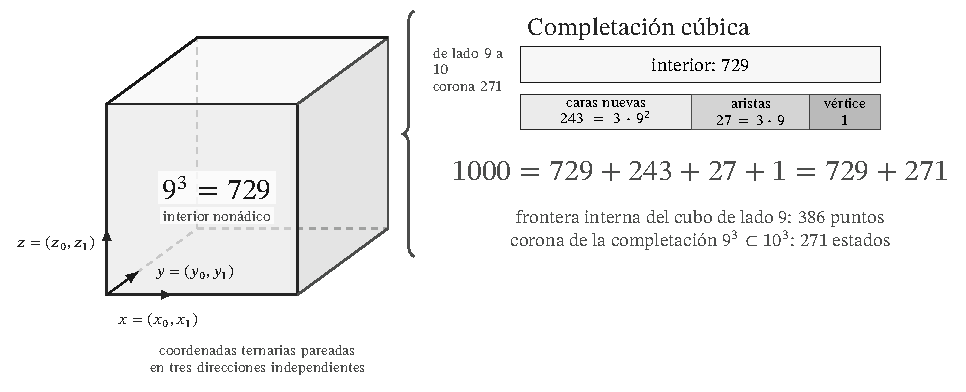
\includegraphics[width=\linewidth]{figures/cubo_emrh.pdf}
\caption{Representación cúbica de la ampliación de nueve a diez clases por coordenada. Los estratos \(S_1,S_2,S_3\) sitúan las incidencias añadidas en caras, aristas y ápice; sus cardinales forman la corona de \(271\) elementos. La frontera de \(386\) elementos pertenece al cubo inicial. La perspectiva geométrica complementa la partición de la figura~\ref{fig:revision-emrh}; las separaciones gráficas tienen función esquemática.}
\label{fig:completacion-cubo-recuperado}
\end{figure}


\subsubsection{Conservación de la unidad y compatibilidad dimensional}

La normalización no se limita a dividir una identidad aislada. En dimensión
\(d\), el producto \(\widehat E^d\) lleva la medida uniforme
\(\mu_d(\{x\})=10^{-d}\). La proyección coordenada
\(p_d:\widehat E^{d+1}\to\widehat E^d\) suprime la última coordenada.

\Needspace{9\baselineskip}
\begin{samepage}
\begin{proposition}[Compatibilidad proyectiva de las medidas normalizadas]
Para todo \(d\geq1\),
\[
 (p_d)_*\mu_{d+1}=\mu_d,
 \qquad \mu_d(\widehat E^d)=1.
\]
La masa del estrato con \(r\) coordenadas adicionales es
\(\binom dr9^{d-r}/10^d\), y la suma de las masas de todos los estratos
es uno.
\end{proposition}
\end{samepage}
\begin{proof}
Cada punto de \(\widehat E^d\) tiene diez preimágenes. Su masa total es
\(10\,10^{-(d+1)}=10^{-d}\). La igualdad para cualquier subconjunto
se obtiene sumando sobre sus puntos. La fórmula estratificada procede
del mismo recuento que \eqref{eq:revision-estratos}; el binomio
\((9+1)^d\) da la normalización total.
\end{proof}

En dimensión tres, retirar el ápice deja masa \(999/1000\), y
restituirlo añade \(1/1000\). Renormalizar antes de la restitución
definiría otra medida: la distinción es operacionalmente relevante.
En particular, conservación de masa probabilística, conservación de los
registros de transporte y disipación termodinámica son afirmaciones con
objetos diferentes. La proposición demuestra la primera y proporciona el
soporte compatible para estudiar la segunda; la tercera requiere una
realización dinámica y energética especificada.

También permanece diferenciada la frontera geométrica interna.
Sobre el representante cartesiano \(\{1,\ldots,9\}^3\), retirar
\(\{2,\ldots,8\}^3\) deja \(386\) puntos. Esta frontera pertenece al
cubo inicial, mientras \(\widehat C\setminus C\) pertenece a su
ampliación. La completación cúbica, la expansión posicional de base mil y
la lectura de incidencia excepcional comparten datos del soporte;
sus mapas respectivos determinan qué información de esos datos utiliza
cada representación.


\subsection{Incidencia cúbica y realización lorentziana}

La completación cúbica aporta una relación entre interior y frontera.
Su geometría puede desarrollarse mediante la incidencia de las seis caras
con los ocho vértices. Etiquetemos las caras por \((i,\varepsilon)\),
\(i\in\{1,2,3\}\), \(\varepsilon\in\{+1,-1\}\), y los vértices por
\(\nu\in\{+1,-1\}^3\). La matriz de incidencia es
\[
 M_{(i,\varepsilon),\nu}=\mathbf1_{\{\nu_i=\varepsilon\}}.
\]
Sean \(u=(1,\ldots,1)^{\mathsf T}\in\RR^6\), \(R_F\) la oposición de
caras y \(P_u=uu^{\mathsf T}/6\), \(P_-=(I-R_F)/2\).

\begin{proposition}[Cociente de incidencia de dimensión cuatro]
El Gramiano de incidencia satisface
\[
 MM^{\mathsf T}=12P_u+4P_-.
\]
Sus autovalores \(12,4,0\) tienen multiplicidades \(1,3,2\).
En consecuencia,
\[
 Q_\square=\RR^6/\ker(MM^{\mathsf T})
 \simeq\RR u\oplus E_-,\qquad E_-=\operatorname{im}P_-.
\]
\end{proposition}
\begin{proof}
Una cara contiene cuatro vértices; dos caras opuestas tienen intersección
vacía, y dos caras distintas no opuestas comparten dos vértices.
La matriz \(12P_u+4P_-\) tiene precisamente esas entradas.
El espacio uniforme tiene dimensión uno; las diferencias entre caras
opuestas generan un espacio de dimensión tres, ortogonal al uniforme.
Su complemento tiene dimensión dos y pertenece al núcleo.
\end{proof}

La descomposición \(1+3\) procede de la incidencia. La elección temporal
se declara mediante la forma bilineal
\[
 B_\square([x],[y])=\langle x,(P_--P_u)y\rangle.
\]
Está bien definida en el cociente, porque ambos proyectores anulan el
núcleo. En la base
\[
 t=[u]/\sqrt6,\qquad
 d_i=[e_{i,+}-e_{i,-}]/\sqrt2,
\]
su matriz es \(\operatorname{diag}(-1,1,1,1)\). Quedan explicitados
el dominio, la descomposición y la convención de signo que producen
la realización de Minkowski. El Gramiano positivo determina el cociente;
la asignación temporal determina la forma indefinida sobre él.

El operador
\[
 W_\square=\sqrt6P_u+\sqrt2P_-,\qquad
 W_\square e_{i,\varepsilon}=t+\varepsilon d_i
\]
envía las seis etiquetas de cara a direcciones nulas, puesto que
\(B_\square(t+\varepsilon d_i,t+\varepsilon d_i)=-1+1=0\).
La inversión de una dirección y la oposición de caras disponen así
de una realización geométrica concreta.

\subsubsection{Soldadura, inversión y subdivisión}

La realización celular utiliza un transporte invertible \(U_m(a)\),
que conserva la forma lorentziana, entre las fibras de los extremos de
una arista dual orientada \(a\), una etiqueta
de cara \(\lambda_m(a)\) y una orientación \(\sigma_m(a)\).
Con \(\ell_m=\ell_0/9^m\), la aplicación de soldadura es
\[
 \beta_m(a)=\ell_m\sigma_m(a)
 W_{\square,s(a)}e_{\lambda_m(a)}.
\]
La inversión compatible satisface
\[
 \beta_m(\bar a)=-U_m(a)\beta_m(a).
\]
Identifiquemos las fibras del origen en dos niveles consecutivos mediante
la isometría de refinamiento declarada. Si los nueve subsegmentos
\(a_1,\ldots,a_9\), de nivel \(m+1\), conservan la etiqueta
y la orientación al ser transportados a esa fibra común, entonces
\begin{equation}
 \beta_m(a)=\sum_{j=1}^9
 U_{m+1}(a_1\cdots a_{j-1})^{-1}\beta_{m+1}(a_j).
 \label{eq:soldadura-refinamiento}
\end{equation}
Cada término transportado equivale a \(\ell_m/9\) por la misma
dirección nula, lo que demuestra la identidad. La hipótesis de
compatibilidad determina qué subdivisiones realizan este refinamiento.
La ecuación reúne dirección, escala y transporte, en lugar de limitar
la correspondencia geométrica a un recuento de dimensiones.

Fijadas además la orientación y la forma lorentziana, la dualidad de
Hodge en \(\Lambda^2Q_\square^*\) satisface \(\star^2=-I\).
En dimensión cuatro, el signo es \((-1)^{2(4-2)+1}=-1\).
Se obtiene una estructura compleja real sobre las dos-formas y,
tras complejificación, los subespacios propios de valores \(+i\) y
\(-i\). La realización electromagnética utilizará este dominio
después de construir la sección electrónica y declarar su acoplamiento.

\subsection{Compatibilidad entre las reducciones modular y posicional}

La base decimal por bloques interviene mediante una división euclídea
que conserva simultáneamente residuo y cociente:
\[
 n=1000q+r,\qquad 0\le r<1000.
\]
Puesto que \(1000\equiv1\pmod9\) y \(1000\equiv1\pmod3\),
\[
 n\equiv q+r\pmod9,\qquad n\equiv q+r\pmod3.
\]
Por tanto, la reducción de un bloque requiere la contribución del
cociente para recuperar la clase del entero. Los números \(0\) y
\(1000\) tienen el mismo resto por \(1000\), pero clases diferentes
por \(9\) y por \(3\). Ésta es una razón operatoria para conservar
la memoria durante el cambio de resolución.

El refinamiento ternario y la determinación de un prefijo decimal
pueden coordinarse mediante un único residuo entero. Si \(N/3^L\)
es un extremo de cilindro y \(D/1000^r\) un extremo decimal, definimos
\[
 A=1000^rN-D3^L.
\]
Al añadir seis símbolos ternarios, \(N'=729N+\nu\),
\(L'=L+6\), con \(0\le\nu<729\). Si el prefijo decimal permanece
fijo, se obtiene
\[
 A'=729A+\nu1000^r.
\]
Si se incorpora además un bloque decimal \(\delta\), entonces
\(D'=1000D+\delta\), \(r'=r+1\), y
\begin{equation}
 A'=729000A+\nu1000^{r+1}-729\delta3^L.
 \label{eq:residuo-dos-bases}
\end{equation}
Ambas identidades se demuestran sustituyendo las definiciones. La
comparación de extremos se reduce así a operaciones enteras que
retienen la contribución de cada prolongación. Esta compatibilidad
es la que permite refinar una región antes de evaluar su coordenada real.

% Incorporación al final de extension.tex; no contiene una sección principal.
% Procedencia: RESULTADO_RECUPERADO; explicitación sectorial de las hipótesis.
% Fuentes leídas: monografía Doble proyección holográfica (cantera editorial),
% manuscrito/local/01_tesis_recuperada.tex y
% manuscrito/generated/algebra_holonomica.tex, especialmente §§1--7 y 21.
% Definición rectora de número: manuscrito/flattened/main_autosuficiente.tex,
% secciones que comienzan en líneas 22137 y 23000 de la cantera de 775 páginas.
% No se adopta su presentación global como prueba de todas las flechas TPK.

\subsection{El número como sección compatible y el valor como lectura}
\label{hist:seccion}

La distinción entre estado y observación permite precisar qué objeto se
prolonga cuando aumenta la resolución. A profundidad \(n\), sea \(X_n\)
el conjunto de estados admisibles producidos por APP--TRIT--TPK. Sus datos
incluyen posición, hojas suma y producto, residuos y cocientes, régimen,
orientación, acarreo, fase, ruta, frontera, memoria y supervivencia. No son
coordenadas independientes: las evaluaciones aritméticas y los transportes
anteriores imponen sus relaciones. Una prolongación conserva esas relaciones
en cada antecedente, aunque añada nuevos pasos y nuevos datos de memoria.
Éste es el sentido de la aritmética de historias desarrollada en
\cite{hmtintegral,hmtholonomia}.

Sean \(r_{m,n}:X_m\to X_n\), para \(m\geq n\), las restricciones de
profundidad, con \(r_{n,n}=\operatorname{id}\) y
\(r_{\ell,n}=r_{m,n}\circ r_{\ell,m}\). Cada restricción conserva el
prefijo y la información ya determinada en él.

\begin{definition}[Sección numérica compatible]
Un número HMT es una historia compatible del sistema de estados:
\begin{equation}
 x=(x_n)_{n\geq0}\in X_\infty:=\varprojlim_n X_n,
 \qquad r_{m,n}(x_m)=x_n.
 \label{hist:limite-inverso}
\end{equation}
Un lector es una operación adicional sobre un dominio especificado de estas
historias. Una cifra es una observación finita; un valor escalar es una
evaluación del lector. El par formado por la sección y su lector constituye
una presentación leída, no una redefinición de la identidad de la sección.
\end{definition}

En el dominio arquimediano \(X_\infty^{\mathrm{Arch}}\), el lector asocia
a cada prefijo un cilindro cerrado, conserva su encajamiento y hace tender
su diámetro a cero. Así determina
\begin{equation}
 \operatorname{ev}_{\mathbb R}:X_\infty^{\mathrm{Arch}}\longrightarrow
 \mathbb R,\qquad
 \{\operatorname{ev}_{\mathbb R}(x)\}=\bigcap_n I_n(x).
 \label{hist:evaluacion}
\end{equation}
La construcción concreta de estos cilindros y la decisión de sus fronteras
se desarrollan en la sección~\ref{sec:generacion}. La definición
\eqref{hist:limite-inverso} no afirma por sí sola que la imagen de
\eqref{hist:evaluacion} sea toda la recta: una afirmación de cobertura
requiere su propio teorema. Tampoco una igualdad de valores establece, sin
un resultado de inyectividad, la igualdad de sus historias. Esta separación
permite hablar de precisión como profundidad conservando la diferencia
entre el antecedente aritmético y su realización escalar.

\subsection{Composición de historias y multiplicador de memoria}
\label{hist:algebra}

Fijemos un sector de estados a profundidad \(n\) y una categoría
\(\mathcal C\) cuyas flechas sean sus historias admisibles. La composición
se escribe \(vu=v\circ u\): primero se recorre \(u\) y después \(v\).
Los pasos elementales proceden de la selección, el transporte y la
actualización del TPK. Una fibra trítica local admite la escritura
\(\mathbb R[J_x]/(J_x^2+\tau(x)1_x)\), donde
\(\tau(x)\in\{+1,0,-1\}\). El régimen y la orientación pertenecen al
estado que se transporta; una transición entre regímenes no equivale a
identificar sus álgebras cuadráticas.

La siguiente formulación precisa un sector algebraico de esa composición.
Para cada objeto \(x\), se da un álgebra real asociativa unitaria \(A_x\),
que puede ser no conmutativa. Para cada \(u:x\to y\), se da un
homomorfismo unital \(\rho_u:A_x\to A_y\). Suponemos una acción estricta:
\begin{equation}
 \rho_{\operatorname{id}_x}=\operatorname{id}_{A_x},\qquad
 \rho_v\rho_u=\rho_{vu}.
 \label{hist:accion-estricta}
\end{equation}
Para cada pareja componible \(u:x\to y\), \(v:y\to z\), fijamos un
multiplicador central invertible
\(\Omega(v,u)\in Z(A_z)^\times\). Se exige la normalización
\(\Omega(\operatorname{id}_y,u)=\Omega(u,\operatorname{id}_x)=1_y\)
y, para cada triple componible, la identidad
\begin{equation}
 \rho_w\bigl(\Omega(v,u)\bigr)\Omega(w,vu)
   =\Omega(w,v)\Omega(wv,u).
 \label{hist:cociclo}
\end{equation}
Son hipótesis explícitas sobre los transportes y sus coeficientes, no una
consecuencia de llamar holonómica a la dinámica. Al aplicar esta presentación
a un sector TPK deben identificarse sus \(\rho_u\) y \(\Omega(v,u)\).
Las transiciones expresadas mediante bimódulos requieren conservar esa
estructura y no quedan reemplazadas por \eqref{hist:accion-estricta}.

El espacio de sumas finitas
\[
 \mathcal H(\mathcal C,A,\rho,\Omega)
   =\bigoplus_{u\in\operatorname{Mor}(\mathcal C)} A_{t(u)}T_u
\]
recibe el producto bilineal
\begin{equation}
 (aT_v)(bT_u)=a\rho_v(b)\Omega(v,u)T_{vu},
 \label{hist:producto}
\end{equation}
si las flechas son componibles, y cero en otro caso. Aquí \(t(u)\)
designa el estado terminal. La suma reúne historias con coeficientes; el
producto concatena historias conservando el multiplicador del registro.

\begin{proposition}[Asociatividad sectorial con multiplicador central]
Bajo \eqref{hist:accion-estricta} y \eqref{hist:cociclo}, el producto
\eqref{hist:producto} es asociativo. Si el conjunto de objetos es finito,
su unidad es \(\sum_x1_xT_{\operatorname{id}_x}\).
\end{proposition}
\begin{proof}
Para \(u:x\to y\), \(v:y\to z\), \(w:z\to t\), sean
\(a\in A_y\), \(b\in A_z\), \(c\in A_t\). Los dos coeficientes
de \(T_{wvu}\) son
\begin{align*}
 ((cT_w)(bT_v))(aT_u):\quad&
 c\rho_w(b)\Omega(w,v)\rho_{wv}(a)\Omega(wv,u),\\
 (cT_w)((bT_v)(aT_u)):\quad&
 c\rho_w(b)\rho_w\rho_v(a)\rho_w(\Omega(v,u))\Omega(w,vu).
\end{align*}
La acción estricta iguala \(\rho_w\rho_v(a)\) con \(\rho_{wv}(a)\).
La centralidad de \(\Omega(w,v)\) permite desplazarlo a la derecha de
ese factor; \eqref{hist:cociclo} iguala entonces los productos restantes.
No se permutan los coeficientes \(a,b,c\). Si el triple no es componible,
ambas parentizaciones son cero por sus estados iniciales y terminales.
La bilinealidad concluye la prueba. Las identidades locales y la
normalización de \(\Omega\) verifican la unidad indicada.
\end{proof}

El acarreo del calendario proporciona un ejemplo efectivo. En la categoría
de un objeto y flechas \(C_9\), tomemos coeficientes
\(A=\mathbb R[z,z^{-1}]\), acción identidad y
\[
 \Omega(b,a)=z^{c_0(a,b)},\qquad
 c_0(a,b)=\left\lfloor\frac{a+b}{9}\right\rfloor,
 \quad 0\leq a,b<9.
\]
Las dos sumas de acarreos de un triple son
\(\lfloor(a+b+c)/9\rfloor\); por ello se cumple
\eqref{hist:cociclo}. La variable formal \(z\) registra la vuelta sin
asignarle un valor numérico. Imponer después \(z^{12}=1\) recupera el
registro dodecafásico del calendario \eqref{eq:extension108}; conservar
\(z\) sin esa relación distingue vueltas sucesivas. El ejemplo realiza
la memoria de este calendario, sin identificarla con la totalidad de la
memoria TPK.

\subsection{Doble varianza del refinamiento y conservación de la unidad}
\label{hist:doble-varianza}

Al restringir estados se prolongan observables en sentido contrario.
Consideremos las álgebras de funciones, con producto puntual,
\(D_n=\operatorname{Fun}(X_n,\mathbb R)\). La precomposición define
\begin{equation}
 r_{m,n}^*:D_n\longrightarrow D_m,
 \qquad r_{m,n}^*f=f\circ r_{m,n}.
 \label{hist:precomposicion}
\end{equation}
Son morfismos unitales; son además inyectivos cuando las restricciones
correspondientes son sobreyectivas. El límite directo
\(D_{\mathrm{cyl}}=\varinjlim_n(D_n,r_{n+1,n}^*)\) reúne las
observaciones de profundidad finita. No se identifica aquí este álgebra
con toda el álgebra de rutas: prolongar los operadores de transporte exige
también sus compatibilidades con el refinamiento.

\begin{lemma}[Unidad y naturalidad de la evaluación]
Si \(e_x\) es el indicador de \(x\in X_n\), se cumple
\begin{equation}
 r_{m,n}^*e_x=\sum_{y:\,r_{m,n}(y)=x}e_y,
 \qquad r_{m,n}^*1_n=1_m,
 \label{hist:unidad}
\end{equation}
y, para todo \(f\in D_n\), \(y\in X_m\),
\[
 \langle r_{m,n}^*f,y\rangle=\langle f,r_{m,n}y\rangle.
\]
Cada sección \(x\in X_\infty\) determina una evaluación bien definida
\(D_{\mathrm{cyl}}\to\mathbb R\), dada por \([f]\mapsto f(x_n)\)
para \(f\in D_n\).
\end{lemma}
\begin{proof}
Las fibras de \(r_{m,n}\) forman una partición de \(X_m\). Sus
indicadores son ortogonales y suman \(1_m\), lo que prueba
\eqref{hist:unidad}. La naturalidad es la definición de precomposición.
Finalmente, \((r_{m,n}^*f)(x_m)=f(x_n)\), de modo que dos representantes
compatibles dan la misma evaluación en el límite directo.
\end{proof}

La unidad global es la función constante uno sobre todas las posibilidades;
la sección individual selecciona una historia compatible. Conservar la
primera no significa inmovilizar la segunda. El refinamiento puede aumentar
la cantidad de extensiones y la profundidad de cada historia manteniendo
la unidad y todas las evaluaciones de sus antecedentes.

\subsection{Retorno de fase, representación de Weyl y dos lecturas}
\label{hist:puente-lecturas}

La ley \eqref{eq:holonomia-memoria} adquiere una realización operatoria
en la suspensión bilateral que se construirá en la
sección~\ref{sec:generacion}. Allí \(T\) es el avance de un paso,
\(V_9\) observa la fase nonádica, \(W_\delta\) la fase de rotación y
\(D_M\) el grado de memoria. Escribiendo
\(\widehat\Gamma_9=T^9\) para la vuelta en esta representación,
las relaciones de Weyl \eqref{eq:weyl-relojes} implican, sobre vectores
de soporte finito,
\begin{equation}
 \begin{aligned}
 V_9\widehat\Gamma_9&=\widehat\Gamma_9V_9,\qquad
 W_\delta\widehat\Gamma_9=e^{2\pi i9\delta}
     \widehat\Gamma_9W_\delta,\\
 [D_M,\widehat\Gamma_9]&=\widehat\Gamma_9.
 \end{aligned}
 \label{hist:tres-retornos}
\end{equation}
La primera igualdad sigue de \(\zeta_9^9=1\); la segunda, de nueve
aplicaciones de la covariancia de \(W_\delta\); la tercera expresa
el incremento unitario de memoria. La fase finita retorna, mientras la
rotación irracional y la memoria distinguen el estado siguiente. Los
caracteres y el parámetro \(\delta\) se realizan después desde la
construcción numérica allí especificada: no seleccionan retrospectivamente
las semillas. Esta representación describe observables y traslaciones de
la suspensión; no reemplaza todas las coordenadas ni todos los operadores
del TPK.

La doble lectura prolonga la misma distinción entre historia y observable.
En su dominio arquimediano se aplica \eqref{hist:evaluacion}; en el
dominio incidencial calibrado, los mapas \(Q_n\) de la
sección~\ref{exc:doble-lectura} conservan las palabras y los marcos de
frontera. La igualdad allí demostrada
\(r_{n,m}Q_n=Q_mp_{n,m}\) determina su prolongación \(Q_\infty\).
Sobre el dominio común de ambas lecturas pueden considerarse conjuntamente
\(\operatorname{ev}_{\mathbb R}(x)\) y \(Q_\infty(x)\): la
primera retiene el valor; la segunda, la incidencia transportada que su
codominio conserva. La sección antecede a ambas. Esta articulación permite
pasar de la aritmética de historias a las constantes y a la lectura
excepcional sin convertir sus realizaciones en nuevos datos iniciales.


\clearpage\section{Generación coinductiva de \texorpdfstring{\(\pi,\varphi,e\)}{pi, phi, e} a profundidad arbitraria}
\label{sec:generacion}

La emisión de seis bloques es una etapa finita de la construcción, no una expansión decimal completa. Su función consiste en producir regiones con multiplicidad, orientación y reglas de transporte. La prolongación debe conservar esos datos y determinar una colección compatible de prefijos de longitud arbitraria. La palabra \emph{generación} designa esta operación; \emph{genealogía} designa la reconstrucción de sus dependencias. Ambas nociones intervienen, pero cumplen funciones distintas.

\subsection{Órbitas, regiones y caracteres de clausura, propagación y autoescala}

Sobre una palabra \(w=(w_1,\ldots,w_6)\), definimos
\[
 r(w)=(w_3,w_1,w_2,w_5,w_6,w_4),\qquad
 s(w)=(w_4,w_5,w_6,w_1,w_2,w_3).
\]
Se cumple \(r^3=s^2=I\) y \(srs=r^{-1}\); por tanto estas permutaciones realizan el grupo diedral \(D_3\). La acción conserva el catálogo y las multiplicidades y conmuta con \(\Psi\). El cociente de las \(243\) palabras visibles tiene \(43\) órbitas: treinta y ocho de cardinal seis y cinco de cardinal tres.

La clase de clausura se reconoce por un predicado de fibra: sus seis orientaciones tienen cinco emisiones por palabra, multiplicidad total \(1008\) y distribución \(432+4\cdot144\). Existe una sola órbita con esas propiedades en el catálogo. Para precisar las otras dos selecciones, escribimos \(f(w)=\#\Psi^{-1}(w)\), \(m(w)=\sum_{U\in\Psi^{-1}(w)}\operatorname{mult}(U)\) y \(\nu(w)=(n_0,n_1,n_2)\). La clase diagonal aditiva de una emisión es \(d(U)=[i+j]_9\) en los índices de cero a ocho; su firma aditiva conserva esta clase y la orientación \(ES\) o \(NO\). Sea \(\mathcal D(\mathcal O)\) el conjunto de esas clases para todas las emisiones sobre una órbita.

Entre las órbitas de tamaño seis, el predicado conjunto
\[
 f(w)=1,\qquad m(w)=144\quad(w\in\mathcal O),\qquad
 \mathcal D(\mathcal O)=\{0,3,6\}
\]
deja exactamente seis órbitas. En este sector, el censo \(\nu=(2,3,1)\), igual al de clausura, selecciona únicamente la propagación; el censo \(\nu=(2,2,2)\) selecciona únicamente la autoescala. El soporte diagonal no puede omitirse: sin él hay cuatro órbitas unipuntuales equilibradas de multiplicidad \(144\), no una. Finalmente, la existencia de una emisión con \(d=6\) y orientación \(ES\) selecciona un representante de cada órbita y conduce a
\begin{equation}
 w^{\rm cl}=010211,\qquad w^{\rm pr}=201101,\qquad w^{\rm au}=121200.
 \label{eq:palabras-regionales}
\end{equation}
Estos símbolos designan primero regiones del catálogo. La identificación escalar se demostrará mediante sus lectores; no se eligen porque coincidan con cifras de una constante conocida.

La palabra de clausura \(010211\) tiene las cinco preimágenes siguientes:
\begin{center}\small
\begin{tabular}{@{}lll r@{}}\toprule
Emisión de seis bloques&Firma multiplicativa&Papel&Multiplicidad\\\midrule
\(501,614,498,169,272,272\)&\(555555\)&transversal&432\\
\(810,923,870,169,272,272\)&\(339555\)&orientación positiva&144\\
\(810,983,810,169,272,272\)&\(393555\)&orientación positiva&144\\
\(870,923,810,169,272,272\)&\(933555\)&orientación positiva&144\\
\(870,923,810,418,674,521\)&\(933717\)&retorno orientado&144\\\bottomrule
\end{tabular}
\end{center}
La multiplicidad \(432\) y la firma constante \(555555\) caracterizan la región transversal. No identifican la posición central \((5,5)\) de APP. Confundir una firma de seis ventanas con una posición del soporte eliminaría la distinción entre región numérica y estructura electrónica.

La microfibra posee además una morfología bipartita precisa. Cada emisión es un producto de una clase de cursor aditivo y una clase multiplicativa. Las tres regiones positivas comparten la misma clase aditiva de dieciocho condiciones; juntas contienen tres clases multiplicativas de ocho condiciones cada una. La región transversal posee un producto \(18\times24\); las tres positivas reunidas, otro \(18\times24\); y el retorno, un producto \(18\times8\). La descomposición por emisiones tiene cinco partes, mientras la descomposición por componentes conexas del grafo bipartito tiene tres. Ambas conservan las mismas \(1008\) semillas sin reducir la forma a un cardinal.

\subsection{Transporte finito y frontera de prolongación}

Los endomorfismos \(L_0,L_1\) del espacio de palabras ternarias actúan antes de la realización arquimediana. Su determinación comienza por las transiciones del estado aritmético, no por la prescripción de dos matrices. Si \(U_t\) es el paso compuesto de selección, transporte y actualización, el bloque observado satisface
\[
 b_j^\chi=\Pi_6(x_j^\chi),\qquad
 x_{j+1}^\chi=U_{9j+9}\cdots U_{9j+1}(x_j^\chi),
 \qquad \chi\in\{\mathrm{cl},\mathrm{pr},\mathrm{au}\}.
\]
Se forman seis transiciones por cada régimen: dos consecutivas en cada una de las tres regiones. Los pares de matrices de orígenes y destinos obtenidos en el registro son
\[
\begin{array}{c|c|c|c}
X_0&Y_0&X_1&Y_1\\\hline
010211&012222&010211&002111\\
012222&010211&002111&110221\\
201101&121221&102011&012222\\
121221&102011&012222&102011\\
121200&112202&121020&010210\\
112202&121020&010210&010200
\end{array}
\]
Cada cadena de seis dígitos representa una fila en \(\FF_3^6\). Puesto que \(\det X_0=1\) y \(\det X_1=-1\) en \(\FF_3\), las ecuaciones \(X_aL_a=Y_a\) determinan unívocamente \(L_a=X_a^{-1}Y_a\). En esa coordenatización de vectores fila resultan
\[
 L_0=\begin{pmatrix}
 2&2&2&1&2&1\\2&1&2&2&1&1\\1&0&0&1&0&2\\
 0&0&1&1&1&0\\2&2&2&0&2&1\\2&1&2&1&0&0
 \end{pmatrix},\quad
 L_1=\begin{pmatrix}
 2&1&2&0&2&2\\1&2&1&1&2&0\\1&2&1&1&1&2\\
 0&1&0&0&2&1\\2&0&2&1&0&1\\0&2&2&2&1&1
 \end{pmatrix}\quad(\bmod3).
\]
El calendario \((L_0,L_0,L_1,L_1)\) produce cuatro nuevos bloques de seis componentes. Sus concatenaciones forman
\[
 w_6\longrightarrow w_{12}\longrightarrow w_{18}
 \longrightarrow w_{24}\longrightarrow w_{30}.
\]
Los subíndices de \(w\) indican longitud acumulada. La frontera \(R_{36}\) conserva la estructura terminal y abre la relación de prolongación; no se renombra como un último bloque periódico que pudiera repetirse indefinidamente.

La identidad \(L=X^{-1}Y\) demuestra unicidad una vez fijadas las transiciones; no sustituye la producción de esas transiciones por \(U_t\). La procedencia de su registro y el examen de los dieciséis calendarios binarios se documentan en el suplemento técnico. El calendario indicado es el único de esos dieciséis que reproduce conjuntamente las tres sucesiones de cinco bloques.

\subsection{Cinco regiones de clausura y compensación angular}

La región de clausura contiene una componente transversal y cuatro acompañantes. El lector simétrico actúa en el espacio de sus cinco posiciones mediante
\[
 P_5=\frac15\mathbf1\mathbf1^{\mathsf T},\qquad
 \mathbf1=(1,1,1,1,1)^{\mathsf T}.
\]
La invariancia \(P_5\lambda=\lambda\) y la conservación \(\mathbf1^{\mathsf T}\lambda=1\) fuerzan \(\lambda=\mathbf1/5\). Esta normalización distribuye la unidad entre posiciones del lector; no sustituye las multiplicidades de semillas \(432,144,144,144,144\) por frecuencias uniformes. La coordenatización elíptica del lector realiza cada coordenada mediante \(1+\lambda_jJ\); su pendiente es \(\lambda_j\), por lo que la pendiente primitiva resulta \(1/5\). Se hace explícita así la regla que pasa de una coordenada normalizada a una pendiente, en lugar de identificar ambas nociones sin mapa. El lector compone las cuatro posiciones acompañantes por la ley
\begin{equation}
 a\oplus b=\frac{a+b}{1-ab}.
 \label{eq:suma-pendientes}
\end{equation}
Esta ley se obtiene al multiplicar \((1+aJ)(1+bJ)\) en el régimen \(J^2=-I\) y dividir por su componente escalar. Por ello la composición de pendientes es una realización de la estructura cuadrática de TRIT, no una suma ordinaria de cuatro fracciones.

\begin{proposition}[Compensador de la clausura]
La composición de cuatro pendientes \(1/5\) es \(120/119\). La condición de retorno a pendiente uno determina un único compensador positivo de la forma \(1/q\), con \(q>1\), y da \(q=239\).
\end{proposition}
\begin{proof}
La primera duplicación da \((1/5)\oplus(1/5)=5/12\); la segunda, \((5/12)\oplus(5/12)=120/119\). La condición
\[
 \frac{120/119-1/q}{1+(120/119)/q}=1
\]
equivale a \((120-119)q=120+119\), por lo que \(q=239\).
\end{proof}

El carácter de clausura resultante tiene realización
\begin{equation}
 \Pi_{\rm cl}=4\left(4\arctan\frac15-\arctan\frac1{239}\right).
 \label{eq:lector-pi}
\end{equation}
La identidad angular de Machin reconoce \(\Pi_{\rm cl}=\pi\). El sentido de la construcción es preciso: la pendiente y el número de composiciones están declarados por el lector de la pentafibra; la ecuación de compensación fuerza \(239\). Una vez producido este carácter, su evaluación por series alternadas no selecciona de nuevo la órbita de semillas.

Para \(0<x<1\), las sumas alternadas
\[
 A_n(x)=\sum_{j=0}^n\frac{(-1)^jx^{2j+1}}{2j+1}
\]
encierran \(\arctan x\) entre dos truncamientos consecutivos, con diferencia \(x^{2n+3}/(2n+3)\). Aplicadas a las dos pendientes de \eqref{eq:lector-pi}, proporcionan extremos racionales de error explícito. El valor numérico se calcula así como consecuencia del carácter exacto, sin introducir un prefijo objetivo.

\subsection{Lector de propagación y normalización de la unidad}

La región de propagación se realiza mediante una colección formal \(P_t\in\mathcal A[[t]]\), donde \(\mathcal A\) es un álgebra conmutativa unitaria sobre \(\QQ\). Su composición satisface \(P_{t+s}=P_tP_s\), con unidad \(P_0=1\), y el transporte elemental orientado fija el generador escalar \(P'_0=+1\). La condición fija su signo, no sólo su magnitud. Escribiendo
\[
 P_t=\sum_{n\ge0}a_nt^n,
\]
la normalización determina \(a_0=a_1=1\). La comparación del coeficiente de \(s^nt\) en \(P_{s+t}=P_sP_t\) da \((n+1)a_{n+1}=a_na_1\); equivalentemente, \(P'_t=P_t\). Así,
\begin{equation}
 (n+1)a_{n+1}=a_n,\qquad a_n=\frac1{n!}.
 \label{eq:propagacion}
\end{equation}
El carácter en una unidad de parámetro es \(\Pi_{\rm pr}=P_1\), reconocido posteriormente como \(e\).

La normalización del generador importa. La ley semigrupal sin ese dato admitiría \(P_t=e^{ct}\) para distintos \(c\); por ello no se omite la condición que fija la unidad del parámetro en el lector. Esta condición es anterior a la comparación decimal y pertenece a la exposición de la regla operacional, no a la elección de un valor experimental.

\begin{proposition}[Cotas racionales de propagación]
Para \(n\ge1\), sea \(E_n=\sum_{j=0}^n1/j!\). Entonces
\[
 E_n<\Pi_{\rm pr}<E_n+\frac{n+2}{(n+1)(n+1)!}.
\]
\end{proposition}
\begin{proof}
El primer término omitido es \(1/(n+1)!\). Cada cociente posterior es a lo sumo \(1/(n+2)\). La suma geométrica mayorante de la cola es
\[
 \frac1{(n+1)!}\frac1{1-1/(n+2)}
 =\frac{n+2}{(n+1)(n+1)!}.
\]
La desigualdad estricta se sigue de la disminución de los cocientes sucesivos.
\end{proof}

\subsection{Incidencia modal y generación de la autoescala}

El selector trítico produce el ciclo \((+1,-1,0)\). En los modos \(\Sigma,\Pi\), la regla es \(+1:m\mapsto\Sigma\), \(-1:m\mapsto\Pi\), \(0:m\mapsto m\). Con cierre cíclico, el modo observado es \((\Sigma,\Pi,\Pi)\). Sus aristas son \(\Sigma\to\Pi\), \(\Pi\to\Pi\) y \(\Pi\to\Sigma\). Por tanto su incidencia, en ese orden de modos, es
\begin{equation}
 F_{\rm av}=\begin{pmatrix}0&1\\1&1\end{pmatrix}.
 \label{eq:fav}
\end{equation}
Las cuatro entradas se obtienen del calendario, no de una ecuación que haya recibido previamente el valor de \(\varphi\). La repetición del calendario da conteos \(3F_{\rm av},9F_{\rm av},36F_{\rm av}\) en longitudes nueve, veintisiete y ciento ocho. Estos conteos no son las potencias de la matriz.

\begin{theorem}[Carácter positivo de autoescala]
La incidencia \eqref{eq:fav} posee un único rayo propio estrictamente positivo. Al normalizarlo como \((1,x)^{\mathsf T}\), su coordenada \(x\) satisface \(x^2-x-1=0\), \(x>0\), y es \(\varphi=(1+\sqrt5)/2\).
\end{theorem}
\begin{proof}
La ecuación propia da \(x=\lambda\) y \(1+x=\lambda x\). Eliminar \(\lambda\) produce el polinomio. De sus dos raíces sólo una es positiva. Como \(F_{\rm av}^2\) tiene todas sus entradas positivas, el rayo positivo es único y simple. La expresión radical reconoce la coordenada obtenida; no participa en la producción de \(F_{\rm av}\).
\end{proof}

Con \(F_0=0,F_1=1,F_{n+1}=F_n+F_{n-1}\), la incidencia induce, para \(n\geq1\),
\[
 F_{\rm av}^n=\begin{pmatrix}F_{n-1}&F_n\\F_n&F_{n+1}\end{pmatrix}.
\]
Los cocientes consecutivos \(F_{n+1}/F_n\) alternan alrededor de \(\varphi\). La identidad de determinante
\[
 F_{n+1}^2-F_nF_{n+2}=(-1)^n
\]
da una anchura exacta \(1/(F_nF_{n+1})\) entre dos cocientes consecutivos. Su crecimiento hace arbitrariamente pequeña esta horquilla racional.

La medida sobre todas las historias compatibles no coincide con la frecuencia de modos del calendario de tres eventos. La frecuencia cronológica es \((1/3,2/3)\). La medida de máxima entropía del envolvente simbólico definido por \(F_{\rm av}\) se construye con sus vectores propios y tiene razón de pesos \(\varphi^{-2}\). Esta última interviene en la lectura areal--volumétrica; no se obtiene sustituyendo sin más una frecuencia de conteo por otra.

Después de generados los caracteres, las dos orientaciones del lector
\[
 R(x,y)=\frac{x}{y^2}
\]
proporcionan
\begin{equation}
 \rho_A=\frac\pi{\varphi^2},\qquad
 \rho_E=\frac\varphi{\pi^2},\qquad
 \varphi^3\rho_A^2\rho_E=1.
 \label{eq:areal-electron}
\end{equation}
La segunda expresión aparecerá en el exponente electrónico. La primera se obtiene también como límite de la lectura marcada \(\pi F_{n-1}/F_{n+1}\). El intercambio de argumentos relaciona ambas, pero no convierte una reparametrización de la ecuación electrónica en una segunda derivación independiente de todos sus coeficientes.

% Articulación posterior a la generación de pi, phi y e.
% Contenido acumulativo; no reemplaza el desarrollo previo del TRIT.
\subsection{Realizaciones exponenciales de las coordenadas generadas}
\label{euler-trit-articulacion}

Las coordenadas regionales ya determinadas permiten reconocer las
realizaciones concretas de la colección cuadrática del TRIT. El orden es
sustantivo: la construcción de las regiones precede a la evaluación de una
exponencial en los parámetros \(\pi\) o \(2\log\varphi\). Estas expresiones
identifican la función de las coordenadas en operadores construidos desde
APP y TPK; no intervienen en la selección de los prefijos que las producen.

\subsubsection{Ciclo ternario, transporte nilpotente e incidencia de hojas}

La multiplicación \(a(r)=4r\) en \(\mathbb Z/9\mathbb Z\) tiene orden
\(3\). Sobre las unidades determina las órbitas \(\{1,4,7\}\) y
\(\{2,8,5\}\). En el módulo de aumento de cualquiera de ellas, formado por
las combinaciones enteras cuyos coeficientes suman cero, la base
\((e_r-e_{4r},e_{4r}-e_{7r})\) da
\[
 C=\begin{pmatrix}0&-1\\1&-1\end{pmatrix},
 \qquad C^2+C+I=0.
\]
La forma restringida tiene matriz de Gram
\(\bigl(\begin{smallmatrix}2&-1\\-1&2\end{smallmatrix}\bigr)\).
En las evaluaciones residuales módulo \(9\), la acción distingue las hojas:
\(S(ax,ay)=aS(x,y)\), mientras \(P(ax,ay)=a^{-1}P(x,y)\).
La realización cíclica conserva, por tanto, una orientación contragrediente
entre suma y producto. Los cocientes del levantamiento entero se conservan
en el registro aritmético correspondiente.

El transporte parabólico elemental se representa mediante
\[
 N=\begin{pmatrix}0&1\\0&0\end{pmatrix}.
\]
La incidencia areal--volumétrica ya construida en \eqref{eq:fav} proporciona
\[
 F_{\rm av}=\begin{pmatrix}0&1\\1&1\end{pmatrix},
 \qquad A=F_{\rm av}^2=\begin{pmatrix}1&1\\1&2\end{pmatrix}.
\]
Los tres operadores actúan en espacios reales declarados: el módulo de
aumento tensorizado con \(\mathbb R\), el plano del transporte nilpotente y
el plano de incidencia modal. Compartir dimensión matricial no identifica
estos espacios ni sus coordenadas.

\begin{proposition}[Generadores concretos de los tres tipos]
\label{euler-trit-generadores}
Los operadores
\[
 J_{\mathrm e}=\frac{2C+I}{\sqrt3},\qquad
 J_{\mathrm p}=N,\qquad
 J_{\mathrm h}=\frac{2A-3I}{\sqrt5}
\]
satisfacen, respectivamente,
\[
 J_{\mathrm e}^{\,2}=-I,\qquad
 J_{\mathrm p}^{\,2}=0,\qquad
 J_{\mathrm h}^{\,2}=I.
\]
\end{proposition}
\begin{proof}
La relación de \(C\) implica \((2C+I)^2=-3I\).
La multiplicación directa da \(N^2=0\).
Finalmente, \(A\) tiene traza \(3\) y determinante \(1\), por lo que
\(A^2-3A+I=0\) y \((2A-3I)^2=5I\).
\end{proof}

\begin{proposition}[Tres evaluaciones de la identidad exponencial]
\label{euler-trit-evaluaciones}
En las realizaciones anteriores,
\begin{equation}
 \boxed{
 \exp(\pi J_{\mathrm e})+I=0,\qquad
 \exp(J_{\mathrm p})=I+J_{\mathrm p},\qquad
 \exp(2\log\varphi\,J_{\mathrm h})=F_{\rm av}^{\,2}.}
 \label{euler-trit-tres-evaluaciones}
\end{equation}
\end{proposition}
\begin{proof}
La especialización elíptica de la exponencial trítica da
\(\cos\pi\,I+\sin\pi\,J_{\mathrm e}=-I\).
La nilpotencia elimina exactamente los términos de grado al menos \(2\)
en la segunda expresión. Para la tercera, \(\varphi^2=\varphi+1\) implica
\[
 \cosh(2\log\varphi)=\frac32,\qquad
 \sinh(2\log\varphi)=\frac{\sqrt5}{2}.
\]
Por tanto, la exponencial vale
\(\frac32I+\frac{\sqrt5}{2}J_{\mathrm h}=A\).
\end{proof}

La primera igualdad representa la media vuelta elíptica; la vuelta completa
satisface \(\exp(2\pi J_{\mathrm e})=I\). La segunda mantiene un término
lineal no nulo: el régimen parabólico expresa transporte, no ausencia de
evolución. La tercera realiza un avance hiperbólico unimodular. Sus
autovalores son \(\varphi^2\) y \(\varphi^{-2}\); una dirección se expande y
la otra se contrae conservando el determinante. Las tres evaluaciones
emplean parámetros distintos de una colección exponencial común.

En esa colección, \(e\) interviene mediante la evaluación escalar
\(\exp(I)=eI\) y la ley \(\exp(sI)\exp(tI)=\exp((s+t)I)\).
Su papel no se restringe al tipo parabólico. La coordenada \(e\), obtenida
previamente de su región, es reconocida aquí como la evaluación unitaria
de la exponencial; esta identidad no sustituye su genealogía coinductiva.

\subsubsection{Resolución polinómica de los regímenes}

Las tres realizaciones admiten una presentación compacta sobre la suma
directa de sus espacios. Defínanse
\[
 \mathbb J=J_{\mathrm e}\oplus J_{\mathrm p}\oplus J_{\mathrm h},
 \qquad Q=\mathbb J^2.
\]
Las relaciones anteriores implican
\[
 \mathbb J^6=\mathbb J^2,\qquad Q^3=Q.
\]
El uso de \(Q\) mantiene separado este cuadrado operatorial del registro
dodecafásico \(K\).

\begin{proposition}[Proyectores polinómicos de régimen]
\label{euler-trit-proyectores}
Las aplicaciones
\[
 p_{\mathrm e}=\frac{Q^2-Q}{2},\qquad
 p_{\mathrm p}=I-Q^2,\qquad
 p_{\mathrm h}=\frac{Q^2+Q}{2}
\]
son idempotentes mutuamente ortogonales, suman \(I\) y recuperan los tres
sumandos de la representación.
\end{proposition}
\begin{proof}
Los tres polinomios toman los valores \((1,0,0)\), \((0,1,0)\) y
\((0,0,1)\) en los puntos \(-1,0,+1\), respectivamente. Las diferencias
entre sus cuadrados y ellos mismos, así como sus productos cruzados, son
múltiplos de \(X^3-X\). Sustituir \(Q\), que anula ese polinomio, demuestra
las identidades. En los tres bloques, \(Q\) actúa como \(-I,0,I\).
\end{proof}

Se obtiene así
\begin{align}
 \exp(t\mathbb J)
 ={}&p_{\mathrm e}(\cos t\,I+\sin t\,\mathbb J)
   +p_{\mathrm p}(I+t\mathbb J)\notag\\
   &+p_{\mathrm h}(\cosh t\,I+\sinh t\,\mathbb J).
 \label{euler-trit-exponencial-total}
\end{align}
Cada sumando conserva su relación cuadrática y la conjugación invierte
su evolución. La representación total reúne los tres regímenes, pero no
define por sí sola un operador de transición entre ellos. Tal transición
requiere los mapas de transporte del TPK con sus dominios, orientación y
memoria. La articulación exponencial permite reconocer sus tipos sin
reemplazar esa dinámica por una identificación de las fibras.

% PROCEDENCIA FOCAL (no impresa)
% Resultado recuperado: tres generadores y tres evaluaciones exponenciales.
% Propietario completo:
% BASE/manuscrito/sections/hmt/09b_algebras_cuadraticas.tex:289-516.
% Antecedente causal de C y acción contragrediente:
% BASE/manuscrito/sections/hmt/03d_esqueleto_ciclotomico_app.tex:13-47,145-246.
% Los tres tipos y la orientación están en:
% BASE/manuscrito/sections/hmt/02_trit_geometrias.tex:83-196.
% Resolución polinómica recuperada:
% output/INVESTIGACION_HOLONOMIA_NONADICA_CRISTAL_APERIODICO_20260903/
% ALGEBRA_HOLONOMICA_UNIVERSAL_Y_EULER_TRITICO.md, secciones 8-11 y 22.
% Los cuatro propietarios se leyeron completos. BASE designa:
% /Users/ruben/Documents/HMT2/
% EL_CIERRE_HOLOGRAFICO_DEL_INFINITO_SUCESOR_102_CAPITULOS_2026-08-28_EN_TRABAJO/
% No se incorpora la identidad P9(alpha)=delta del documento especializado:
% esa identificación no pertenece a este bloque.
% Tampoco se identifica una dirección nilpotente con la vacancia electrónica,
% ni se presume una representación global del transporte por la suma directa.
% COMPROBACIONES: Python estándar, enteros y Fraction.
% C^2+C+I=0; (2C+I)^2=-3I; N^2=0; (2Fav^2-3I)^2=5I.
% 81 pares de residuos verifican las dos acciones contragredientes.
% Los 3 proyectores se verificaron en Q=-1,0,+1; prueba general en texto.
% 6 labels únicos y entornos equilibrados. Sin compilación.


\subsection{Cilindros compatibles y profundidad arbitraria}

La realización de un bloque ternario \(b=(b_1,\ldots,b_6)\) es el entero
\[
 \nu(b)=\sum_{j=1}^6b_j3^{6-j}\in\{0,\ldots,728\}.
\]
Una sucesión de bloques define prefijos enteros por \(N_{n+1}=729N_n+\nu(b_{n+1})\), comenzando en \(N_0=m\), donde \(m\) es la parte entera determinada por el lector. Las horquillas anteriores sitúan los caracteres de clausura, propagación y autoescala en \((3,4)\), \((2,3)\) y \((1,2)\), respectivamente; por tanto, sus valores iniciales son \(m=3,2,1\). Los bloques siguientes refinan la parte fraccionaria. El cilindro correspondiente es
\begin{equation}
 I_n=\left[\frac{N_n}{729^n},\frac{N_n+1}{729^n}\right],
 \qquad |I_n|=729^{-n}.
 \label{eq:cilindro}
\end{equation}
La convención semiabierta se utiliza para seleccionar un representante cuando un valor cae en una frontera. Para el paso al límite se utilizan las clausuras de estos intervalos y se identifican las dos expansiones fronterizas equivalentes. Esta precisión impide suponer que toda intersección de intervalos semiabiertos encajados sea automáticamente no vacía.

\begin{theorem}[Determinación de la realización escalar]
Una historia de bloques compatible determina un único límite de los extremos izquierdos de \eqref{eq:cilindro}. Si un carácter exacto dispone de horquillas racionales de anchura arbitrariamente pequeña y se separa de la frontera de cada cilindro decimal examinado, cada prefijo decimal de longitud finita se determina después de un cálculo finito. Los prefijos así obtenidos son compatibles entre sí.
\end{theorem}
\begin{proof}
La extensión de un bloque conserva el prefijo anterior por división euclídea. Los cilindros cerrados están encajados y su diámetro tiende a cero; sus extremos izquierdos son de Cauchy y tienen un único límite. Para una longitud decimal fijada, un valor separado de las fronteras de la partición posee distancia positiva a ellas. Una horquilla suficientemente estrecha queda contenida en una única celda y determina su prefijo. La unicidad de la celda y el encajamiento de las particiones prueban la compatibilidad por truncamiento. En los puntos con expansión terminal debe añadirse la decisión exacta de frontera y su convención de representación; no se deduce esa decisión de una anchura numérica solamente.
\end{proof}

Los caracteres de clausura, propagación y autoescala poseen las horquillas anteriores. Tras su reconocimiento, la irracionalidad de \(\pi,e,\varphi\) garantiza su separación de las fronteras racionales de cualquier precisión decimal finita. La profundidad arbitraria significa \emph{para todo horizonte finito existe un cálculo que determina su prefijo}; no exige que una máquina finita almacene de una vez una cantidad infinita de cifras. El objeto matemático es la colección compatible completa, y una ejecución produce una proyección finita de ella.

\subsection{Involución especular y sincronización de las regiones}

La conexión nonádica transporta conjuntamente los tres caracteres. En la coordenatización de la novena fase, el eje de autoescala y la suma ternaria de clausura y propagación permanecen fijados bajo el intercambio especular. La inversión helicoidal cambia el sentido del transporte; el espejo de los dos canales cambia su orientación relativa. Son involuciones diferentes, aunque ambas actúen sobre el mismo sistema de trayectorias.

Las coincidencias de censo ilustran esa coordinación:
\begin{center}
\begin{tabular}{@{}c rrr l@{}}\toprule
Fase&\(N_\pi\)&\(N_e\)&\(N_\varphi\)&Igualdad de conteos\\\midrule
4&207&207&122&\(N_\pi=N_e\)\\
5&39&151&151&\(N_e=N_\varphi\)\\
6&110&110&69&\(N_\pi=N_e\)\\
7&81&29&81&\(N_\varphi=N_\pi\)\\
8&59&59&59&sincronización triple\\
9&43&43&43&sincronización triple\\\bottomrule
\end{tabular}
\end{center}
Estos enteros cuentan coordenadas compatibles de las regiones. No afirman una igualdad entre \(\pi\), \(e\) y \(\varphi\) como números reales. Si
\[
 \partial(a,b,c)=(a-b,b-c,c-a),
\]
su imagen pertenece al retículo \(A_2=\{(u,v,w)\in\ZZ^3:u+v+w=0\}\). En las fases ocho y nueve la componente relativa se anula, pero la componente diagonal cambia de \((59,59,59)\) a \((43,43,43)\). La sincronización relativa coexiste con un desplazamiento de \(-16\) por canal. El cierre que conducirá a \(\alpha\) debe conservar ambas informaciones: coincidencia relativa y evolución de la memoria.

\subsection{Suspensión helicoidal esturmiana}

La relación entre las bases nueve y diez de la completación define el parámetro adimensional
\begin{equation}
 \delta=\frac{\log(10/9)}{\log10}.
 \label{eq:delta-sturm}
\end{equation}
No se obtiene de una constante física objetivo. Es la escala logarítmica relativa de dos bases ya presentes en la construcción. Su empleo como lectura simbólica del refinamiento tiene una consecuencia exacta.

\begin{lemma}[Irracionalidad de la pendiente]
El número \(\delta\) es irracional.
\end{lemma}
\begin{proof}
Si \(\delta=p/q\), \(q>0\), entonces \((10/9)^q=10^p\) y \(9^q=10^{q-p}\). La factorización del primer miembro contiene el primo tres y la del segundo sólo los primos dos y cinco. La igualdad es imposible.
\end{proof}

La palabra mecánica inferior, con intercepto \(\theta\), es
\[
 z_n(\theta)=\lfloor(n+1)\delta+\theta\rfloor-\lfloor n\delta+\theta\rfloor\in\{0,1\}.
\]
Se obtiene al observar la rotación \(\theta\mapsto\theta+\delta\pmod1\) mediante el intervalo \([1-\delta,1)\). La sucesión de eventos tiene densidad \(\delta\), y la suma sobre cualquier ventana de longitud \(L\) vale \(\lfloor L\delta\rfloor\) o \(\lceil L\delta\rceil\). Como \(21<1/\delta<22\), las separaciones entre eventos son veintiuno o veintidós. La palabra que indica cuáles son los intervalos cortos es otra palabra mecánica de pendiente \(\sigma=22-1/\delta\); sus eventos están separados por seis o siete intervalos primarios. La segunda escala es inducida por la primera y no un segundo parámetro libre.

% Desarrollo reunido de DESARROLLO_MATEMATICO, apartados 38--40 y 50.
\subsubsection{Índice de capacidad, vacancias e inducción del régimen trítico}
\label{vac-capacidad-trit}

La sucesión de vacancias está vinculada al refinamiento mediante una
identidad de incrementos. Para mostrarla se fija el origen de fase
\(\theta=0\). Sean
\[
 \rho=\log_{10}9=1-\delta,\qquad
 \mathcal C_t=\lfloor(t+1)\rho\rfloor\quad(t\geq0).
\]
El índice \(\mathcal C_t\) expresa la capacidad decimal del refinamiento
en la normalización que compara un bloque ternario de \(6\) posiciones,
con \(729\) posibilidades, y un bloque decimal de \(3\) posiciones, con
\(1000\) posibilidades. En efecto,
\(\log_{1000}729=\log_{10}9=\rho\). Se reserva la letra \(K\) para
el registro dodecafásico que se construirá posteriormente.

\begin{proposition}[Complementariedad de capacidad y vacancia]
\label{prop:capacidad-vacancia}
Para \(t\geq1\),
\begin{equation}
 \mathcal C_t-\mathcal C_{t-1}=1-z_t(0).
 \label{eq:capacidad-vacancia}
\end{equation}
En consecuencia, si \(0\leq a<b\),
\[
 \mathcal C_b-\mathcal C_a+
 \sum_{t=a+1}^{b}z_t(0)=b-a.
\]
\end{proposition}
\begin{proof}
La irracionalidad de \(\delta\) da
\[
 \mathcal C_t
 =t+1-\lceil(t+1)\delta\rceil
 =t-\lfloor(t+1)\delta\rfloor.
\]
La resta de dos términos consecutivos produce
\eqref{eq:capacidad-vacancia}. La suma sobre el intervalo es telescópica.
\end{proof}

Cada transición aumenta en una unidad el contador de bloques. Si
\(z_t=0\), aumenta también la capacidad; si \(z_t=1\), la capacidad se
mantiene mientras se incorpora una transición a la historia. La vacancia
es aquí un evento de retención de capacidad, con una posición y un
antecedente determinados. El balance anterior conserva exactamente la
longitud entre capacidad adquirida y vacancias registradas. La fase
observada \(g_t^{\rm cap}=[\mathcal C_t]_9\) satisface
\[
 g_t^{\rm cap}-g_{t-1}^{\rm cap}\equiv1-z_t\pmod9.
\]
Esta fase de capacidad y la fase cronológica \([t]_9\) son dos
observaciones diferentes. Una retención local de capacidad y una vuelta
completa de la holonomía tienen mecanismos distintos, aunque ambas
permitan conservar la observación de fase con modificación del estado.

La relación con TRIT puede seguirse en las propias posiciones de vacancia.
Para \(j\geq1\), defínanse
\[
 p_j=\left\lfloor\frac j\delta\right\rfloor,\qquad
 v_j=\mathcal C_{p_j},\qquad h_j=p_{j+1}-p_j.
\]
La desigualdad \(p_j\delta<j<(p_j+1)\delta\) identifica \(p_j\)
como la posición del evento \(j\). Como \(0<\delta<1\), da también
\(\lfloor(p_j+1)\delta\rfloor=j\), y por tanto
\[
 v_j=p_j-j,\qquad
 v_{j+1}-v_j=h_j-1.
\]
Si \(s_j=22-h_j\), entonces \(s_j\in\{0,1\}\) y
\begin{equation}
 [v_{j+1}]_3=[v_j-s_j]_3.
 \label{eq:vacancia-regimen}
\end{equation}
Un intervalo de longitud \(22\) conserva la clase; uno de longitud
\(21\) la desplaza una unidad en sentido negativo. El selector canónico
se aplica a la fase positiva \(r_j=1+[v_j]_9\):
\[
 \tau_j=M_{\rm ph}(r_j).
\]
Queda determinado así un régimen trítico por el índice de capacidad
retenido en cada evento, además de la codificación binaria de la vacancia.

Las posiciones de los intervalos cortos forman la codificación mecánica
inducida de pendiente \(22-1/\delta\). Sus separaciones \(6\) y \(7\)
determinan las longitudes de las mesetas de la clase \([v_j]_3\), una
vez fijados el origen y la convención de extremos. Las primeras clases
son \(2\) durante \(6\) eventos, \(1\) durante \(7\) y \(0\) durante
\(7\); el primer tramo de \(6\) es la restricción inicial de una meseta.
Sus firmas recorren \(0,-1,+1\). Las ecuaciones
\eqref{eq:capacidad-vacancia} y \eqref{eq:vacancia-regimen} explicitan el
enlace entre refinamiento, vacancias y selección del régimen. La lectura
cuadrática del TRIT realiza después esos tipos mediante sus respectivos
generadores; el acontecimiento temporal y su representación geométrica
conservan así una dependencia identificable.

La inversión del índice monótono proporciona otra observación útil:
\[
 \mathcal T(k)=\min\{t:\mathcal C_t=k\}
   =\left\lceil\frac k\rho\right\rceil-1\qquad(k\geq1).
\]
Si \(\sigma=\rho^{-1}-1\), el número de bloques necesarios para ganar
\(m\) unidades de capacidad es
\[
 \mathcal T(k+m)-\mathcal T(k)
 =m+\lceil(k+m)\sigma\rceil-\lceil k\sigma\rceil
 \in\{m+\lfloor m\sigma\rfloor,m+\lceil m\sigma\rceil\}.
\]
En particular, \(9\) unidades de capacidad requieren \(9\) o \(10\)
bloques. El período de una fase finita permanece exacto, mientras el
tiempo de retorno medido por el otro índice admite dos valores. Esta
distinción es parte de la dinámica del refinamiento y no una corrección
de sus valores numéricos a posteriori.


\begin{theorem}[Complejidad de las lecturas de fase]
Para \(m\ge1\), la palabra mecánica tiene complejidad factorial \(p(m)=m+1\). Al conservar la fase \(n\bmod9\), la complejidad es \(p_9(m)=9(m+1)\); al conservar sólo su clase ternaria, es \(p_3(m)=3(m+1)\). Las tres entropías topológicas son nulas.
\end{theorem}
\begin{proof}
Los predecesores de los dos extremos del intervalo de codificación forman, para factores de longitud \(m\), \(m+1\) puntos distintos de la circunferencia: la coincidencia entre extremos desplazados elimina las duplicaciones y la irracionalidad impide coincidencias adicionales. Esos puntos determinan \(m+1\) intervalos de itinerario constante y distintos. Toda órbita irracional visita cada intervalo, de donde \(p(m)=m+1\).

Fijada una fase módulo nueve, las posiciones de esa fase recorren una rotación de paso \(9\delta\), también irracional. Por densidad aparecen todos los factores en cada fase, y la primera coordenada distingue sus nueve copias. El mismo argumento con paso \(3\delta\) da tres copias tras la reducción ternaria. Finalmente, \(m^{-1}\log(c(m+1))\to0\) para \(c=1,3,9\).
\end{proof}

El producto de fases \(C_9\times\mathbb T\), trasladado por \((1,\delta)\), tiene caracteres de frecuencia
\[
 \frac a9+k\delta\pmod1,\qquad a\in\ZZ/9\ZZ,\ k\in\ZZ.
\]
El módulo espectral no es \(\log10\): es el módulo aditivo generado por \(1/9\) y \(\delta\), módulo los enteros. El factor \(\log10\) pertenece a la normalización de \eqref{eq:delta-sturm}.

Una presentación operatoria hace explícita la memoria. En \(\ell^2(\ZZ)\), sea \(T|n\rangle=|n+1\rangle\), \(V_9|n\rangle=\zeta_9^n|n\rangle\), \(W_\delta|n\rangle=e^{2\pi i n\delta}|n\rangle\) y \(D_M|n\rangle=\lfloor n/9\rfloor|n\rangle\). Sobre vectores de soporte finito,
\begin{equation}
 V_9T=\zeta_9TV_9,\qquad
 W_\delta T=e^{2\pi i\delta}TW_\delta,\qquad
 [D_M,T^9]=T^9.
 \label{eq:weyl-relojes}
\end{equation}
Las dos primeras relaciones son covariancias de Weyl; la tercera expresa que una vuelta nonádica aumenta el grado de memoria. La rotación de base es abeliana, mientras el álgebra de observables y traslaciones no lo es. La inversión \(|n\rangle\mapsto|-n\rangle\) conjuga el avance con el retroceso. Esta realización proporciona una suspensión helicoidal aperiódica con retorno finito de fase, no una palabra periódica de longitud nueve.

\begin{figure}[htbp]
\centering
\begin{tikzpicture}[x=1cm,y=1cm,>=Latex,font=\small]
\begin{scope}[xshift=1.8cm,yshift=.3cm]
\draw[->,gray] (0,-.5)--(0,3.65) node[above] {\(n/9\)};
\foreach \k in {0,1,2,3}{
 \draw[gray!60,dashed] (-1.1,\k)--(1.1,\k);
 \node[left,font=\scriptsize] at (-1.1,\k){\(\k\)};
}
\draw[black,line width=.65pt,domain=0:27,samples=260,smooth,variable=\n]
 plot ({cos(40*\n)},{\n/9+.14*sin(40*\n)});
\foreach \n in {0,...,27}{
 \fill ({cos(40*\n)},{\n/9+.14*sin(40*\n)}) circle (.026);
}
\foreach \k in {0,1,2,3}{\fill (1,\k) circle (.045);}
\node[align=center,text width=3.3cm,font=\scriptsize] at (0,-1.02)
 {Misma fase en \(n=0,9,18,27\);\\grado de memoria distinto.};
\end{scope}
\begin{scope}[xshift=4.2cm,yshift=.5cm]
\node[anchor=west] at (0,3.1){\(z_n(0)=\lfloor(n+1)\delta\rfloor-\lfloor n\delta\rfloor\)};
\draw[->] (0,1.7)--(9,1.7) node[right]{\(n\)};
\foreach \n in {21,43,65,87,109,131,152,174,196,218}{
 \draw[line width=.6pt] ({\n*.039},1.7)--({\n*.039},2.25);
 \fill ({\n*.039},2.25) circle (.033);
 \node[below,font=\tiny] at ({\n*.039},1.7){\n};
}
\foreach \a/\b/\g in {21/43/22,43/65/22,65/87/22,87/109/22,109/131/22,131/152/21,152/174/22,174/196/22,196/218/22}{
 \node[font=\scriptsize] at ({(\a+\b)*.0195},2.55){\g};
}
\node[anchor=west,align=left,text width=8.3cm] at (0,.55)
 {La codificación irracional determina los intervalos entre eventos. El retorno de la fase nonádica no convierte esta secuencia en una palabra periódica.};
\end{scope}
\end{tikzpicture}
\caption{Representaciones complementarias del transporte. A la izquierda, proyección de la hélice \((\cos(2\pi n/9),\sin(2\pi n/9),n/9)\): el avance de nueve pasos recupera la fase e incrementa la altura. A la derecha, los diez primeros eventos de la palabra inferior para \(\delta=\log_{10}(10/9)\), con separaciones exactas \(21\) o \(22\). La representación helicoidal no introduce una métrica física adicional.}
\label{fig:holonomia-esturmiana}
\end{figure}


Para este recuento fijamos el intercepto \(\theta=0\) y los extremos acumulados \((N_0,\ldots,N_4)=(0,729,972,999,1000)\), correspondientes al orden cúbico \((729,243,27,1)\). Los conteos inferiores son \(\lfloor N_j\delta\rfloor-\lfloor N_{j-1}\delta\rfloor\), y dan \((33,11,1,0)\). Los superiores son \(\lceil N_j\delta\rceil-\lceil N_{j-1}\delta\rceil\), con la misma frontera inicial cero, y dan \((34,11,1,0)\). Estos valores dependen del intercepto y del orden de los estratos; no se afirman para una fase inicial arbitraria. Sus totales son cuarenta y cinco y cuarenta y seis. El incremento corresponde a una única unidad de frontera, situada en el primer estrato de esta partición ordenada. Las cifras treinta y cuatro y once aparecen así en un mismo recuento previo a toda coordenatización de unidades; identificarlas con exponentes físicos exige, además, la derivación dimensional correspondiente.

La denominación \emph{cristal aperiódico} se emplea aquí para este orden simbólico, con complejidad, espectro y retorno especificados. La entropía topológica nula no equivale por sí sola a disipación física nula: una realización termodinámica necesita una dinámica energética y una operación de borrado definidas. Del mismo modo, esta lectura esturmiana no sustituye a todos los operadores del TPK ni demuestra por sí sola la periodicidad o aperiodicidad de la salida completa de \(\alpha\). Su función es hacer explícita una estructura de orden que el simple retorno del calendario no describe.

% Adición acumulativa. Insertar después de la suspensión esturmiana existente.
% Conservar íntegro el texto y la figura fig:holonomia-esturmiana.
\subsection{Conexión nonádica, holonomía y representación monodrómica}
\label{mono-ampl:conexion}

La estructura regional requiere distinguir el transporte que produce una
historia, la observación de su fase y la representación de sus retornos.
APP aporta las dos evaluaciones aritméticas con residuo y cociente; TRIT
determina el régimen y la orientación; el Topological Phase Kernel compone
selección, transporte y actualización. Las condiciones iniciales de
cardinal \(104\,976\), su catálogo de \(468\) emisiones y las \(243\)
palabras visibles en el ambiente de \(729\) elementos pertenecen a etapas
distintas de esa construcción. La cadena
\[
 w_6\longrightarrow w_{12}\longrightarrow w_{18}
 \longrightarrow w_{24}\longrightarrow w_{30}
 \longrightarrow R_{36}\longrightarrow G_9
\]
conduce a una conexión conjunta sobre las tres regiones. Sus nueve fases
son posiciones de un mismo transporte, y las coordenadas regionales
\(\pi,\varphi,e\), junto con la determinación dodecafásica de \(\alpha\),
proceden de sus lecturas compatibles\cite{hmtintegral,hmtholonomia}.

En el índice de prolongación \(k\), una coordenatización del estado conserva
\[
 \widehat x_k=(B_k,C_k,p_k,c_k,\Sigma_k,W_k,g_k,m_k).
\]
Aquí \(B_k\) reúne los tres bloques regionales, \(C_k\) es el cilindro,
\(p_k\) el prefijo, \(c_k\) el registro de acarreo, \(\Sigma_k\) la firma
de frontera y \(W_k\) la información incidencial. La fase es
\(g_k=1+[(k-1)]_9\); \(m_k\) cuenta las vueltas completas. La reducción
\(\beta_k=[m_k]_{12}\) conserva la posición dodecafásica, mientras el
entero \(m_k\) distingue sus sucesivas vueltas.

\begin{definition}[Transporte de una vuelta nonádica]
\label{mono-ampl:def-vuelta}
Sean \(\mathcal R_k\subseteq\widehat X_k\times\widehat X_{k+1}\)
las relaciones de extensión admisible del TPK. La realización de la
holonomía en el nivel \(k\) es la composición relacional
\[
 \Gamma_{9,k}=\mathcal R_{k+8}\circ\cdots\circ\mathcal R_k.
\]
Para \(s\geq1\), su prolongación a \(s\) vueltas es
\[
 \Gamma_{9s,k}=
 \Gamma_{9,k+9(s-1)}\circ\cdots\circ\Gamma_{9,k}.
\]
\end{definition}

La formulación relacional conserva las continuaciones admisibles. Sobre
una historia individualizada, cada flecha lleva al estado efectivamente
prolongado; el bloque visible aislado puede seguir admitiendo más de una
continuación. Esta diferencia es precisamente la función de la memoria y
de las condiciones de frontera en la determinación de la trayectoria.

\begin{proposition}[Iteración del retorno y memoria acumulada]
\label{mono-ampl:vueltas}
En toda composición admisible de \(s\) vueltas,
\[
 g_{k+9s}=g_k,\qquad m_{k+9s}=m_k+s,\qquad
 \beta_{k+9s}=\beta_k+s\pmod{12}.
\]
\end{proposition}
\begin{proof}
La regla de una vuelta conserva la fase e incrementa el contador en una
unidad. Su aplicación al estado ya transportado repite exactamente esas
dos operaciones. La inducción da las dos primeras igualdades; reducir la
segunda módulo \(12\) da la tercera.
\end{proof}

El contador proporciona así un testigo entero de la diferencia entre las
vueltas. Tras \(12\) vueltas la pareja de fases finitas se restaura, pero
el contador aumenta \(12\). La extensión no escindida
\eqref{eq:extension108} expresa la composición del calendario mediante su
cociclo; la trayectoria conserva además la elevación entera de ese dato.
La conservación significa aquí transporte de las contribuciones previas,
no inmovilidad de todas las coordenadas.

\subsubsection{Representación bilateral del índice de retorno}

La realización geométrica del grafo cíclico admite una representación
operatoria especialmente simple. Numeramos aquí las fases de \(0\) a
\(8\), mediante un desplazamiento del origen respecto de \(g_k\), y
escribimos \(k=9m+r\), con \(0\leq r<9\), en la recta entera
que recubre el ciclo de fases. Sobre
\(\mathcal H_{\rm ind}=\ell^2(\mathbb Z)\), la base
\(|k\rangle=|r,m\rangle\) permite expresar el desplazamiento unitario
\[
 T|r,m\rangle=
 \begin{cases}
 |r+1,m\rangle,&r<8,\\
 |0,m+1\rangle,&r=8.
 \end{cases}
\]
La inversa reduce \(r\) en una unidad cuando \(r>0\), y lleva
\(|0,m\rangle\) a \(|8,m-1\rangle\). El paso por el origen de fase
incorpora, por tanto, la unidad exacta de cociente.

\begin{proposition}[Representación de la monodromía del ciclo]
\label{mono-ampl:representacion}
Sea \(S=T^9\). Entonces
\[
 S|r,m\rangle=|r,m+1\rangle,\qquad
 \mathbb Z\longrightarrow\mathcal U(\mathcal H_{\rm ind}),
 \quad s\longmapsto S^s
\]
es una representación unitaria fiel del grupo de vueltas del ciclo.
\end{proposition}
\begin{proof}
Nueve desplazamientos conservan el resto de la división por \(9\) e
incrementan el cociente. Las potencias satisfacen
\(S^{s+t}=S^sS^t\), y \(S^s|r,m\rangle=|r,m+s\rangle\) distingue
todo entero \(s\). La permutación de una base ortonormal es unitaria.
\end{proof}

Esta representación corresponde al recubrimiento del ciclo, cuyo grupo
de vueltas es \(\mathbb Z\), y representa la fase con su contador. El
estado del TPK contiene además las coordenadas de trayectoria ya descritas.
La extensión bilateral admite índices negativos como coordenadas del
recubrimiento; una trayectoria iniciada en una condición inicial utiliza
su semieje admisible. De este modo se dispone de una inversa operatoria
del índice sin convertir cada relación de extensión en una biyección del
estado completo.

Con \(D_M|k\rangle=\lfloor k/9\rfloor|k\rangle\), la identidad
\([D_M,S]=S\) expresa el incremento de memoria en el dominio denso de
vectores de soporte finito. Si \(\mathcal I|k\rangle=|-k\rangle\) y
\(P_0\) proyecta sobre los índices divisibles por \(9\), se obtiene
además
\begin{equation}
 \mathcal I T\mathcal I=T^{-1},\qquad
 \mathcal I D_M\mathcal I=-D_M-(I-P_0).
 \label{mono-ampl:inversion-contador}
\end{equation}
En efecto, para \(k=9m+r\),
\(\lfloor-k/9\rfloor=-m\) si \(r=0\) y vale \(-m-1\) si \(r>0\).
La inversión conserva así el término de frontera de la división euclídea.

\subsection{Reloj de bloques y reloj de capacidad}
\label{mono-ampl:relojes}

El índice de una aplicación de refinamiento y el número de posiciones
decimales disponibles tienen leyes relacionadas, pero diferentes. Para
expresarlas reservamos \(n\) al índice de bloques ternarios y definimos
\[
 \rho=\log_{1000}729=\log_{10}9,\qquad
 \delta=1-\rho,\qquad
 \mathcal C_n=\lfloor(n+1)\rho\rfloor,\quad n\geq0.
\]
La letra \(\mathcal C_n\) designa aquí la capacidad, no el registro
dodecafásico \(K\). En el origen de fase canónico, la palabra mecánica
anterior proporciona
\[
 Z_n=\sum_{j=0}^{n}z_j(0)=\lfloor(n+1)\delta\rfloor.
\]

\begin{proposition}[Balance exacto entre capacidad y vacancias]
\label{mono-ampl:balance-capacidad}
Para \(n\geq0\) y, en la segunda identidad, \(n\geq1\),
\[
 \mathcal C_n=n-Z_n,\qquad
 \mathcal C_n-\mathcal C_{n-1}=1-z_n(0).
\]
\end{proposition}
\begin{proof}
La irracionalidad de \(\delta\) implica
\(\lceil(n+1)\delta\rceil=\lfloor(n+1)\delta\rfloor+1\).
Entonces
\[
 \lfloor(n+1)(1-\delta)\rfloor
 =n+1-\lceil(n+1)\delta\rceil=n-Z_n.
\]
Restar dos identidades consecutivas concluye la prueba.
\end{proof}

Un evento \(z_n=1\) añade un bloque a la historia manteniendo la capacidad
\(\mathcal C_n\); un evento \(z_n=0\) incrementa ambos contadores. En
cualquier intervalo, los incrementos de capacidad y las vacancias suman
exactamente su longitud. Reduciendo módulo \(q\), para \(q=9\) o
\(q=108\), resulta
\[
 [\mathcal C_n]_q=[n]_q-[Z_n]_q.
\]
La fase uniforme de bloques y la fase de capacidad se relacionan mediante
la memoria integrada de vacancias. En particular, una retención de
capacidad y una vuelta completa de la conexión tienen mecanismos
distintos, aunque ambas puedan conservar una observación de fase.

La inversión monótona del reloj da un tiempo de primera llegada:
\[
 T_{\rm cap}(a)=\min\{n:\mathcal C_n=a\}
 =\left\lceil\frac a\rho\right\rceil-1,
 \qquad a\geq1.
\]
Con \(\sigma=\rho^{-1}-1\), el tiempo empleado en ganar \(b\) unidades
de capacidad es
\[
 T_{\rm cap}(a+b)-T_{\rm cap}(a)
 =b+\lceil(a+b)\sigma\rceil-\lceil a\sigma\rceil.
\]
La diferencia de techos toma uno de los dos enteros adyacentes a
\(b\sigma\). Así se obtienen \(9\) o \(10\) bloques para ganar
\(9\) unidades de capacidad, y \(113\) o \(114\) para ganar \(108\).
Son tiempos del reloj inverso, medidos desde una primera llegada; el
contador de vueltas se interpreta siempre en el índice al que pertenece.

\subsection{Suspensión simbólica y cristal temporal aperiódico}
\label{mono-ampl:cristal}

La codificación por rotación reúne periodicidad de fase, recurrencia local
y aperiodicidad global. Sea \(\mathcal X_\delta\subseteq\{0,1\}^{\mathbb Z}\)
la clausura, en la topología producto, de las traslaciones de la palabra
bilateral \(z_n(\theta)\). Denotemos por \(\sigma_{\rm sh}\) el
desplazamiento de sus sucesiones. Conservando una fase nonádica, el paso es
\[
 F(r,z)=([r+1]_9,\sigma_{\rm sh}z),\qquad
 (r,z)\in C_9\times\mathcal X_\delta.
\]

\begin{definition}[Cristal temporal aperiódico simbólico]
\label{mono-ampl:def-cristal}
La suspensión de techo unitario del sistema anterior es el espacio
\[
 \mathcal S_\delta=
 \bigl((C_9\times\mathcal X_\delta)\times\mathbb R\bigr)/\sim,
 \qquad (y,t+1)\sim(Fy,t),
\]
con flujo \(\Phi_s[y,t]=[y,t+s]\). Se denomina \emph{cristal temporal
aperiódico simbólico} a este modelo de orden temporal, junto con su
codificación de vacancias y la representación del contador de vueltas.
\end{definition}

El adjetivo temporal designa la acción del flujo y de su sección de retorno;
la aperiodicidad caracteriza sus itinerarios. La frecuencia de unos de cada
sucesión es \(\delta\): la cota uniforme de discrepancia menor que uno,
obtenida por telescopía en cualquier ventana, persiste al tomar la clausura.
Una sucesión periódica tendría frecuencia racional. Por tanto,
\(\mathcal X_\delta\) no contiene órbitas periódicas. La suspensión
tampoco tiene órbitas cerradas: un retorno del flujo exigiría un tiempo
entero y una periodicidad del itinerario.

Las palabras finitas sí reaparecen. Los itinerarios de longitud \(m\)
proceden de una partición de la circunferencia por \(m+1\) puntos; cada
intervalo es visitado recurrentemente por la rotación irracional. Incluso
al restringir los tiempos a una fase fija, el paso \(9\delta\) sigue
siendo irracional. Ésta es la razón de que cada palabra aparezca en las
\(9\) fases y de las complejidades ya establecidas
\[
 p(m)=m+1,\qquad p_9(m)=9(m+1),\qquad p_3(m)=3(m+1).
\]
La recurrencia de configuraciones locales coexiste con la ausencia de un
período global. Su entropía topológica es nula porque estas complejidades
crecen linealmente.

La realización por los observables \(V_9,W_\delta\) y el desplazamiento
\(T\) expresa el mismo orden mediante las covariancias
\eqref{eq:weyl-relojes}. Las frecuencias del reloj uniforme pertenecen a
\(\frac19\mathbb Z+\delta\mathbb Z\), módulo \(1\). El reloj de
capacidad conserva adicionalmente la relación
\([\mathcal C_n]_9=[n]_9-[Z_n]_9\); no se sustituye por la fase uniforme
al interpretar los retornos. El término \emph{cristal temporal} queda así
definido mediante un sistema dinámico matemático. Su realización física
requiere especificar una dinámica energética, sus observables temporales
y su estabilidad, datos distintos de la construcción simbólica presente.

\subsection{Simetría especular de las regiones y doble realización}
\label{mono-ampl:regiones}

El intercambio especular actúa en el bloque regional
\(B=(u^\pi,u^e,u^\varphi)\in(\mathbb F_3^6)^3\) por
\[
 \mathfrak cB=(u^e,u^\pi,u^\varphi).
\]
Su eje fijo y su agregado son, respectivamente, \(u^\varphi\) y
\(s=u^\pi+u^e\). Esta fijación se refiere a la involución en una fibra;
ambas coordenadas pueden evolucionar durante el transporte nonádico.
Con \(q=u^\pi+u^e+u^\varphi\),
\(a=u^\pi+u^e-u^\varphi\) y \(d=u^\pi-u^e\), se recupera
\[
 u^\varphi=2(q-a),\qquad s=q-u^\varphi,\qquad
 u^\pi=2(s+d),\qquad u^e=2(s-d).
\]
Las igualdades son componente a componente en \(\mathbb F_3\), donde
\(2^{-1}=2\). El espejo conserva \(q,a,s\) e invierte \(d\); esta
coordenada antisimétrica individualiza el reparto que el agregado conserva
sin distinguir. La inversión \(\mathcal I\) del índice temporal y la
involución \(\mathfrak c\) de canales actúan, por consiguiente, sobre
datos diferentes.

El retorno de fase posee un testigo explícito:
\[
 \begin{aligned}
 B_1&=(012222\mid121221\mid112202),\\
 B_{10}&=(101222\mid112221\mid112002).
 \end{aligned}
\]
Las dos posiciones tienen fase \(1\); el bloque, el eje y la memoria han
cambiado. Asimismo, la sincronización de los censos en las fases \(8\) y
\(9\) anula sus diferencias relativas, mientras la componente diagonal
pasa de \((59,59,59)\) a \((43,43,43)\). La igualdad de un observable
relativo no agota el estado que lo determina.

La doble realización conserva esa arquitectura. En la sección
\ref{exc:doble-lectura}, el mismo prefijo determina por una parte cilindros
encajados y por otra una sucesión de palabras codificadas con sus marcos.
El primer mapa pasa al límite por contracción de diámetros; el segundo
satisface \(r_{n,m}Q_n=Q_mp_{n,m}\) y define \(Q_\infty\).
La figura \ref{mono-ampl:fig-regional} anticipa esas dos aplicaciones.
El recorrido incidencial posterior construye códigos, retículos y la
realización de Moonshine en sus dominios propios; el grupo de automorfismos
actúa sobre esa realización, no sobre las cifras por una identificación
implícita.

% Figura acumulativa; destino figures/monodromia_regional_ampliacion.tex.
\begin{figure}[!htbp]
\centering
\begin{tikzpicture}[x=1cm,y=1cm,>=Latex,font=\small,
  flow/.style={->,line width=.55pt},
  ann/.style={align=center,font=\footnotesize}]
\node[font=\bfseries] at (6.9,9.2)
  {Conexión nonádica y coordenadas regionales};
\begin{scope}[shift={(3.4,6.8)}]
 \foreach \k in {1,...,9}{
  \pgfmathsetmacro{\ang}{90-40*(\k-1)}
  \coordinate (p\k) at (\ang:1.52);
  \fill (p\k) circle (1.4pt);
  \node[fill=white,inner sep=1.1pt,font=\footnotesize]
    at (\ang:1.83) {\(\k\)};
 }
 \foreach \k in {1,...,8}{
  \pgfmathtruncatemacro{\next}{\k+1}
  \draw[flow,shorten >=3pt,shorten <=3pt] (p\k)--(p\next);
 }
 \draw[flow,shorten >=3pt,shorten <=3pt] (p9)--(p1);
 \node[ann] at (0,.1) {\(g_k\in C_9\)\\\(\Gamma_{9,k}\)};
 \node[ann] at (0,-2.23) {Una vuelta: \(g\mapsto g\), \(m\mapsto m+1\)};
\end{scope}
\node[ann,text width=5.25cm] at (10.1,7.75)
 {\(B_k=(u_k^\pi,u_k^e,u_k^\varphi)\)\\
 bloque regional en una fibra};
\node at (8.55,6.5) {\(u^\pi\)};
\node at (11.65,6.5) {\(u^e\)};
\draw[<->,line width=.65pt] (8.95,6.5)--node[above]{\(\mathfrak c\)}(11.25,6.5);
\draw[densely dashed,gray] (10.1,5.72)--(10.1,7.23);
\node[fill=white,inner sep=2pt] at (10.1,5.6){\(u^\varphi\)};
\node[ann] at (10.1,4.6)
 {Eje \(u^\varphi\) y agregado \(u^\pi+u^e\)\\
 invariantes bajo \(\mathfrak c\)};
\draw[flow] (5.45,6.8)--(7.25,6.8);
\draw[gray!60,line width=.3pt] (.55,4.02)--(13.25,4.02);
\node[ann,text width=12cm] (hist) at (6.9,3.47)
 {Historia compatible: prefijos, cilindros, orientación, cocientes,
 marcos de incidencia y memoria};
\coordinate (fork) at (6.9,2.85);
\draw[flow] (hist.south)--(fork);
\draw[flow] (fork)--(3.6,2.2);
\draw[flow] (fork)--(10.3,2.2);
\node[ann,text width=5.6cm] at (3.6,1.65)
 {Realización arquimediana\\
 \(I_{n+1}\subseteq I_n,\quad |I_n|=729^{-n}\)\\
 límite de los prefijos regionales};
\node[ann,text width=5.6cm] at (10.3,1.65)
 {Realización incidencial\\
 \(r_{n,m}Q_n=Q_mp_{n,m}\)\\
 palabras codificadas y marcos compatibles};
\node[ann,text width=5.6cm] at (3.6,.42)
 {\(\pi,\varphi,e\); determinación dodecafásica de \(\alpha\)};
\node[ann,text width=5.6cm] at (10.3,.42)
 {Witt--Golay--Leech--\(V^\natural\)\\
 automorfismos de la realización excepcional};
\draw[flow] (3.6,1.03)--(3.6,.78);
\draw[flow] (10.3,1.03)--(10.3,.78);
\end{tikzpicture}
\caption{\fontsize{9}{11}\selectfont Nueve fases de una conexión y dos realizaciones de la historia
compatible. El ciclo representa la fase; cada vuelta incrementa el contador.
El diagrama regional representa la involución \(\mathfrak c\), que
intercambia clausura y propagación y fija el eje de autoescala en una fibra.
Esta invariancia no impone que el eje sea constante durante el transporte.
Las dos aplicaciones inferiores utilizan el mismo prefijo: una determina
su límite numérico y la otra conserva palabras y marcos de incidencia. Los
mapas de esta segunda realización se especifican en la sección
\ref{exc:doble-lectura}; el recorrido excepcional se desarrolla después.}
\label{mono-ampl:fig-regional}
\end{figure}


\subsection{Transporte temporal y composición exponencial trítica}
\label{mono-ampl:euler}

Las relaciones de Euler de la sección \ref{euler-trit-articulacion}
describen las realizaciones locales de los tres regímenes. Para una firma
fija \(\tau\), el generador satisface \(J_\tau^2=-\tau I\); la
conjugación algebraica lleva \(J_\tau\) a \(-J_\tau\). En consecuencia,
\[
 \exp(sJ_\tau)\exp(tJ_\tau)=\exp((s+t)J_\tau),\qquad
 \overline{\exp(tJ_\tau)}=\exp(-tJ_\tau),
\]
y el producto de una evolución con su conjugada es la unidad. En el tipo
elíptico se realiza mediante \(\cos^2t+\sin^2t=1\); en el hiperbólico,
mediante \(\cosh^2t-\sinh^2t=1\); en el parabólico,
\((I+tN)(I-tN)=I\), pues \(N^2=0\). La misma ley de conservación
admite tres expresiones cuadráticas.

La realización elíptica cierra una vuelta; la nilpotente conserva un
desplazamiento lineal; la hiperbólica separa expansión y contracción con
determinante unitario. En los parámetros regionales ya generados,
\[
 \exp(\pi J_{\mathrm e})=-I,\qquad
 \exp(J_{\mathrm p})=I+J_{\mathrm p},\qquad
 \exp(2\log\varphi\,J_{\mathrm h})=F_{\rm av}^{\,2}.
\]
La evaluación \(\exp(I)=eI\) reconoce la unidad de la ley exponencial
común. El número \(e\) no se asigna exclusivamente al régimen parabólico.

El transporte de una realización local por un isomorfismo \(U\) conserva
estas relaciones: si \(J'=UJU^{-1}\), la serie exponencial da
\(U\exp(tJ)=\exp(tJ')U\). La identidad transporta el régimen y su
norma. Una transición entre tipos cuadráticos diferentes pertenece, en
cambio, a la selección de hojas y regímenes del TPK; no es una conjugación
que cambie el valor de \(J^2\). El producto temporal conserva por ello el
orden de las transiciones y la información de sus extremos.

Esta articulación distingue la clausura de una representación local y la
holonomía de una historia. Puede cumplirse \(\exp(2\pi J_{\mathrm e})=I\)
al mismo tiempo que \(S|r,m\rangle=|r,m+1\rangle\). La primera igualdad
restaura la orientación del régimen; la segunda registra otra vuelta. La
estructura discreta conserva ambas: el retorno local y la procedencia
acumulada del estado que lo realiza.


% Recuperación del producto nativo y su selector, no incorporación de RH.
\subsection{Irreducibilidad multiplicativa y períodos de retorno}
\label{primos-retornos}

La distinción entre estructura, evaluación y fase aparece también en el
sector multiplicativo. El producto local de APP contiene tanto el residuo
como el cociente; su iteración permite construir formas normales y
factorizaciones antes de examinar sus períodos decimales. Este desarrollo
sitúa la expresión \emph{modo primo} en un dominio preciso y relaciona la
irreducibilidad con las operaciones ya definidas, no con una coincidencia
aislada de períodos \cite{hmtintegral,hmtholonomia}.

Sea
\[
 \mathcal W_9=\{\varnothing\}\sqcup
 \bigsqcup_{\ell\geq1}\{1,\ldots,9\}^{\ell}.
\]
Las secuencias se ordenan desde el dígito menos significativo. La evaluación
\(\operatorname{ev}_9(u)=\sum_j u_j9^j\), con
\(\operatorname{ev}_9(\varnothing)=0\), es biyectiva sobre los enteros no
negativos: para un entero positivo, la división de \(n-1\) por \(9\)
determina de manera única el primer dígito y la continuación. Esta es la
numeración nonádica biyectiva; conserva el representante \(9\) de la
frontera.

La suma \(\boxplus_\#\) se obtiene aplicando la hoja aditiva de APP a los
dígitos de cada posición y propagando sus cocientes. Si sólo hay un dígito,
éste constituye el residuo provisional; un cociente entrante no nulo se
normaliza mediante una segunda operación aditiva. La suma de los
cocientes se transporta a la posición siguiente. Para multiplicar una
secuencia por un dígito \(d\), la celda multiplicativa produce
\(u_jd=9q_j+r_j\), y el cociente entrante \(c_j\) se incorpora mediante
\[
 (w_j,c_{j+1})=
 \begin{cases}
 (r_j,q_j),&c_j=0,\\
 \bigl(R^+(r_j,c_j),q_j+q^+(r_j,c_j)\bigr),&c_j>0.
 \end{cases}
\]
Se comienza con \(c_0=0\) y se incorpora el cociente final cuando es no
nulo. Durante la suma, \(c_j\leq2\); durante el producto por un dígito,
\(c_j\leq9\). Las operaciones locales reciben así argumentos dentro
de su dominio. Denotemos por \(d\odot_\#u\) este segundo procedimiento,
con \(d\odot_\#\varnothing=\varnothing\).

Para \(v=(v_0,\ldots,v_{m-1})\), el producto completo se construye por
la recurrencia
\[
 a_m=\varnothing,\qquad
 a_j=(9\odot_\#a_{j+1})\boxplus_\#(v_j\odot_\#u),
 \qquad u\boxtimes_\#v=a_0.
\]
La regla compone las dos hojas locales. Su evaluación verifica
\begin{equation}
 \operatorname{ev}_9(u\boxtimes_\#v)
   =\operatorname{ev}_9(u)\operatorname{ev}_9(v).
 \label{eq:primos-entrelazamiento}
\end{equation}
En efecto, cada transición conserva la suma parcial más el cociente
pendiente ponderado por la potencia de \(9\). La recurrencia da entonces
\(\operatorname{ev}_9(a_j)=9\operatorname{ev}_9(a_{j+1})+
v_j\operatorname{ev}_9(u)\), cuya iteración prueba
\eqref{eq:primos-entrelazamiento}. La unicidad de la forma normal transporta
asociatividad y conmutatividad al producto construido; su unidad es \((1)\).

\begin{definition}[Coproducto multiplicativo reducido]
Sobre el espacio vectorial de soporte finito generado por las formas
normales no vacías se define
\[
 \widetilde\Delta_\# e_w
 =\sum_{\substack{u\boxtimes_\#v=w\\u,v\ne(1)}}e_u\otimes e_v.
\]
Una forma normal no unitaria es irreducible cuando su imagen por
\(\widetilde\Delta_\#\) es nula.
\end{definition}

Las fibras de factorización son finitas por
\eqref{eq:primos-entrelazamiento}. En la completación
\(\mathcal H_\#=\ell^2(\mathcal W_9\setminus\{\varnothing\})\),
las imágenes de formas distintas tienen soportes disjuntos. Si
\(d_\#(w)\) cuenta las factorizaciones ordenadas no unitarias, el dominio
de la clausura es
\[
 \operatorname{Dom}(\overline{\widetilde\Delta_\#})
 =\left\{x\in\mathcal H_\#:
       \sum_w d_\#(w)|x_w|^2<\infty\right\}.
\]
En efecto, la norma cuadrada de la imagen es esa suma ponderada. Por ello,
el operador
\[
 A_\#=(\overline{\widetilde\Delta_\#})^*
                  \overline{\widetilde\Delta_\#}
\]
es diagonal, positivo y autoadjunto: su valor propio en \(e_w\) es el
número de factorizaciones ordenadas no unitarias de \(w\). La proyección
\[
 P_{\rm irr}=(I-|e_{(1)}\rangle\langle e_{(1)}|)
                    \mathbf1_{\{0\}}(A_\#)
\]
selecciona exactamente las formas irreducibles. Mediante la evaluación
multiplicativa, éstas corresponden a los primos ordinarios. La selección
depende de la estructura de factorización, y mantiene separado el estado
unitario.

Para un valor \(n\geq2\) coprimo con \(10\), la división decimal induce la
permutación de residuos \(r\mapsto10r\pmod n\). El retorno del residuo
\(1\) tiene período
\[
 \tau_n=\operatorname{ord}_n(10).
\]
Si \(n=\prod_p p^{a_p}\), el teorema chino de los restos da
\[
 \tau_n=\operatorname{mcm}_{p^{a_p}\parallel n}
                    \operatorname{ord}_{p^{a_p}}(10).
\]
El retorno compuesto sincroniza los retornos de las potencias primas.
Para un primo \(p\notin\{2,3,5\}\), se tiene
\[
 \tau_p\mid p-1,\qquad
 M_p=\frac{10^{\tau_p}-1}{p}\in\mathbb N,
 \qquad M_p\equiv0\pmod9.
\]
La última congruencia expresa el cierre nonádico de la repetición decimal:
\(10^{\tau_p}-1\) es múltiplo de \(9\) y \(p\) es invertible módulo
\(9\). La misma congruencia vale para cualquier \(n\) coprimo con
\(90\). En particular, \(7,13,77,91,143\) tienen período decimal \(6\),
aunque sólo los dos primeros son irreducibles. El coproducto y el período
registran, por tanto, propiedades diferentes de un mismo valor construido.

Esta diferenciación precisa la relación con el refinamiento aperiódico.
La secuencia de vacancias determina los incrementos del índice de
capacidad; la factorización determina los modos multiplicativos; la
división decimal determina sus tiempos de retorno. El representante
nonádico conserva el cierre de fase, mientras que el cociente y la
factorización conservan información que ese cierre no distingue. El
enlace con las construcciones espectrales del tratado reside en esos
operadores y sus entrelazamientos. La demostración de sus resultados
analíticos posteriores mantiene su desarrollo propio; no se sustituye por
la periodicidad de una observación residual.

\subsubsection{Discrepancia de vacancias y lecturas de Dirichlet}

El vínculo admite también una expresión analítica exacta. Se conserva la
misma codificación \(z_n=z_n(0)\), para \(n\geq1\), y se consideran
dos observables posteriores: la serie sobre todos los índices y el
producto sobre los índices seleccionados por irreducibilidad. Para
\(\operatorname{Re}s>1\),
\[
 Z_{\rm vac}^{+}(s)=\sum_{n\geq1}\frac{z_n}{n^s},\qquad
 Z_{\rm vac}^{\times}(s)=\prod_p(1-p^{-s})^{-z_p}.
\]
Ambos convergen absolutamente en ese semiplano. Su factor común es la
densidad \(\delta\), pero sus discrepancias son diferentes.

\Needspace{21\baselineskip}
\begin{proposition}[Separación de la densidad de vacancias]
Se tiene
\[
 Z_{\rm vac}^{+}(s)=\delta\zeta(s)+H_{\rm vac}(s),
 \qquad H_{\rm vac}\in\mathcal O(\operatorname{Re}s>0).
\]
En \(\operatorname{Re}s>1\), con logaritmos definidos por las series
absolutamente convergentes de Euler,
\[
 Z_{\rm vac}^{\times}(s)=\zeta(s)^\delta G_{\rm vac}(s),\qquad
 \log G_{\rm vac}(s)=
 \sum_p(z_p-\delta)\log(1-p^{-s})^{-1}.
\]
\end{proposition}
\begin{proof}
Las sumas parciales centradas satisfacen
\[
 A_N:=\sum_{n=1}^N(z_n-\delta)
 =\lfloor(N+1)\delta\rfloor-N\delta,\qquad |A_N|<1.
\]
La sumación de Abel representa el término centrado por
\(s\int_1^\infty A_{\lfloor x\rfloor}x^{-s-1}\,dx\). La integral
converge localmente de manera uniforme en \(\operatorname{Re}s>0\),
lo que prueba la holomorfía. La segunda identidad resulta de separar
\(z_p=\delta+(z_p-\delta)\) en el logaritmo del producto, dentro de
su dominio de convergencia absoluta.
\end{proof}

La descomposición hace visible qué añade la lectura sobre primos: examina
la misma sucesión de vacancias sobre un subconjunto determinado por la
factorización. El control de la discrepancia sobre todos los enteros da
la primera prolongación holomorfa; el segundo observable conserva una
discrepancia propia sobre primos. Son dos aplicaciones de la misma
estructura discreta, con dominios analíticos expresos. Esta articulación
explica su pertinencia en el núcleo aritmético sin trasladar a este
artículo la demostración de los resultados terminales del tratado.


\clearpage% BEGIN NUCLEO_ADITIVO_20260921_SELECCION
\clearpage
% Ampliación demostrativa DF003--DF007. No modifica la fuente integral.
% Propietario común de los archivos Lean citados en estos comentarios:
% output/PAQUETE_ARTICULO_I_INTEGRACION_ESTADO_CAMPOS_20260919/.
% Residencia causal de la primera sección: después de los lectores regionales
% coinductivos y antes de emplear sus registros como entrada de la selección K.
% Residencia causal de la segunda sección: después de la construcción marcada
% Paley--Witt--Golay--Leech y antes de la reconstrucción de la estructura VOA.
% Los dos cortes expositivos conservan el mismo origen APP--TRIT--TPK.

\section[Generación regional y refinamiento]{Compatibilidad integral de la generación regional, el refinamiento cilíndrico y la incidencia}
\label{act21:sec:df-lectores-cilindros}

La prolongación regional produce sucesiones ordenadas de bloques, junto con
sus profundidades de lectura. La proyección arquimediana y la incidencia
ternaria se calculan sobre esas mismas sucesiones. El vínculo entre ambas
realizaciones puede formularse enteramente mediante operaciones enteras:
selección por intervalos racionales, división euclídea, elevación de seis
trits, lectura de acarreo y transformación de Witt. Esta formulación permite
seguir cada coeficiente desde su bloque generador hasta su empleo posterior.

La construcción utiliza los tres lectores regionales ya obtenidos del estado
APP--TRIT--TPK. Los denotaremos por los índices
\(c\in\{\mathrm P,\mathrm E,\mathrm F\}\), correspondientes, respectivamente,
a las regiones de clausura, propagación y autoescala. Su realización real se
escribirá \(v_c\). Las identificaciones posteriores
\(v_{\mathrm P}=\pi_{\mathrm{HMT}}\),
\(v_{\mathrm E}=e_{\mathrm{HMT}}\) y
\(v_{\mathrm F}=\varphi_{\mathrm{HMT}}\) conservan ese orden causal.
La operación que emite un bloque inspecciona los intervalos racionales del
lector regional; el valor real interviene en la demostración de corrección
de dicha operación.

\subsection{Emisión posicional mediante separación racional de celdas}
\label{act21:subsec:df-emision-racional}

% Fuente: lean/biblioteca/RegionalPublicationComposition.lean,
% produced_brackets, eventual_publication, joint_eventual_publication,
% search_terminates, stopped_cell_correct, publications_compatible.

Para cada región se dispone de dos sucesiones racionales
\(\ell_c(j),u_c(j)\), construidas por su lector, que cumplen
\[
 \ell_c(j)\leq v_c\leq u_c(j).
\]
La propiedad de separación de celdas demostrada para esos lectores afirma
que, para cada entero \(s>0\), existe \(J\) tal que, para todo \(j\geq J\),
\begin{equation}
 \lfloor s\ell_c(j)\rfloor
 =\lceil su_c(j)\rceil-1
 =\lfloor sv_c\rfloor.
 \label{act21:eq:df-separacion-celdas}
\end{equation}
La evitación de las fronteras racionales por los valores regionales es la
hipótesis de los teoremas previos que garantiza esta separación. Aquí se
emplea su conclusión operativa, con los lectores y los intervalos que la
producen.

\begin{definition}[Índice de separación y prefijo emitido]
Para \(s>0\), sea
\[
 j_c(s)=\min\{j\in\mathbb N:
 \lfloor s\ell_c(j)\rfloor=\lceil su_c(j)\rceil-1\}.
\]
Para una base entera \(b\geq2\) y una profundidad \(n\geq0\), se define
\begin{equation}
 P_c(b,n)=\lfloor b^n\ell_c(j_c(b^n))\rfloor.
 \label{act21:eq:df-publicacion-prefijo}
\end{equation}
El prefijo contiene la parte entera y las primeras \(n\) posiciones en base
\(b\); por consiguiente, \(P_c(b,0)\) es la parte entera regional.
\end{definition}

\begin{theorem}[Terminación y corrección de la emisión]
\label{act21:thm:df-emision-correcta}
El índice \(j_c(s)\) existe para todo \(s>0\). Los prefijos emitidos cumplen
\begin{equation}
 P_c(b,n)=\lfloor b^n v_c\rfloor,
 \qquad
 P_c(b,n)\leq b^n v_c<P_c(b,n)+1.
 \label{act21:eq:df-prefijo-correcto}
\end{equation}
Para cada escala \(s\) puede elegirse además un único índice de suficiencia
\(J(s)\) válido simultáneamente para las tres regiones.
\end{theorem}

\begin{proof}
La igualdad eventual de \eqref{act21:eq:df-separacion-celdas} hace no vacío el
conjunto que define \(j_c(s)\). Su mínimo existe por buen orden de
\(\mathbb N\). En cualquier índice donde se produzca la igualdad, la cota
inferior racional proporciona
\(\lfloor s\ell_c(j)\rfloor\leq\lfloor sv_c\rfloor\).
La cota superior, junto con la evitación de una frontera de celda, da
\(\lfloor sv_c\rfloor\leq\lceil su_c(j)\rceil-1\).
Al coincidir ambos extremos enteros, el entero intermedio coincide con
ellos. Esto demuestra \eqref{act21:eq:df-prefijo-correcto}. Para la afirmación
conjunta basta tomar el máximo de los tres índices de suficiencia obtenidos
para la misma escala. El índice conjunto controla simultáneamente las tres
emisiones, mientras que cada región conserva sus propios intervalos.
\end{proof}

\begin{proposition}[Compatibilidad exacta de los prefijos]
\label{act21:prop:df-prefijos-compatibles}
Para \(n,m\geq0\),
\begin{equation}
 \left\lfloor\frac{P_c(b,n+m)}{b^m}\right\rfloor=P_c(b,n).
 \label{act21:eq:df-truncamiento}
\end{equation}
En particular, el bloque siguiente
\(d_c(b,n)=P_c(b,n+1)\bmod b\) satisface
\begin{equation}
 P_c(b,n+1)=bP_c(b,n)+d_c(b,n),\qquad 0\leq d_c(b,n)<b.
 \label{act21:eq:df-paso-posicional}
\end{equation}
\end{proposition}

\begin{proof}
Escribamos \(b^n v_c=N+\theta\), con
\(N=P_c(b,n)\) y \(0\leq\theta<1\). Entonces
\(P_c(b,n+m)=b^mN+\lfloor b^m\theta\rfloor\), y el segundo sumando
pertenece a \(\{0,\ldots,b^m-1\}\). La división euclídea por \(b^m\)
recupera \(N\). La especialización \(m=1\) produce
\eqref{act21:eq:df-paso-posicional} y su cota residual.
\end{proof}

\subsection{Bloques regionales de seis trits a profundidad arbitraria}
\label{act21:subsec:df-bloques-arbitrarios}

% Fuente: deltas/integracion/JointRegionalFrontier.lean,
% publish_base729_eq_base3, generated_block_from_longer_prefix,
% generated_block_eq_finite, generated_signature_eq_finite.

La igualdad entera \(729=3^6\) determina la agrupación de seis posiciones
ternarias en un bloque. Para \(t\geq0\), definimos
\begin{equation}
 u_c(t)=P_c(729,t+1)\bmod729,
 \qquad
 B_{c,j}(t)=
 \left\lfloor\frac{u_c(t)}{3^{5-j}}\right\rfloor\bmod3,
 \quad 0\leq j<6.
 \label{act21:eq:df-bloque-y-banda}
\end{equation}
De este modo, \(B_c(t)\) es una palabra ordenada de seis trits y
\begin{equation}
 u_c(t)=\sum_{j=0}^{5}B_{c,j}(t)3^{5-j}.
 \label{act21:eq:df-elevacion-banda}
\end{equation}
La palabra y su elevación entera son dos representaciones mutuamente
recuperables del mismo bloque emitido.

\begin{theorem}[Estabilidad de extracción a cualquier profundidad]
\label{act21:thm:df-bloque-estable}
Se cumplen, para todo \(n\),
\[
 P_c(729,n)=P_c(3,6n).
\]
Si \(t<n\), entonces
\begin{equation}
 u_c(t)=
 \left\lfloor\frac{P_c(729,n)}{729^{n-t-1}}\right\rfloor\bmod729.
 \label{act21:eq:df-bloque-prefijo-largo}
\end{equation}
En consecuencia, cualquier ampliación del prefijo preserva todos los
bloques previamente emitidos y todas las firmas que se calculan sobre ellos.
\end{theorem}

\begin{proof}
La primera igualdad resulta de que ambos prefijos se separan a la misma
escala, \(729^n=3^{6n}\), y del
teorema~\ref{act21:thm:df-emision-correcta}. Para la segunda aplicamos
\eqref{act21:eq:df-truncamiento} a las profundidades \(n\) y \(t+1\), y después
tomamos el residuo módulo \(729\). La extracción ternaria de
\eqref{act21:eq:df-bloque-y-banda} es determinista. Cualquier función explícita
de esas dieciocho coordenadas conserva, por tanto, el mismo resultado al
ampliar el prefijo.
\end{proof}

La construcción está cuantificada sobre \(t\in\mathbb N\). Una tabla que
materialice cien bloques constituye una evaluación finita de esta
construcción; la fórmula \eqref{act21:eq:df-bloque-prefijo-largo} determina
exactamente su compatibilidad con cualquier extensión posterior.

\begin{example}[Primer bloque conjunto]
La evaluación de los lectores regionales seleccionados da las palabras
\[
 B_{\mathrm P}(0)=010211,\qquad
 B_{\mathrm E}(0)=201101,\qquad
 B_{\mathrm F}(0)=121200.
\]
Su elevación por \eqref{act21:eq:df-elevacion-banda} produce
\[
 u_{\mathrm P}(0)=103,\qquad
 u_{\mathrm E}(0)=523,\qquad
 u_{\mathrm F}(0)=450.
\]
Por ejemplo,
\(201101_3=2\cdot243+27+9+1=523\).
Las seis posiciones, incluidos los ceros iniciales, se conservan en la
representación de banda. El cero inicial de \(010211\) tiene una posición
definida aunque la escritura decimal de \(103\) carezca de él.
\end{example}

\subsection{Registros de transición y reconstrucción de las elevaciones lineales}
\label{act21:subsec:df-registros-transicion}

% Fuentes: deltas/integracion/RegionalTransitionRecords.lean y
% GeneratedTransitionRecords.lean; lean/biblioteca/TPKLifts.lean.
% Los enlaces reconstruidos son R(0)->R(1) y R(2)->R(3).

Sobre \(\mathbb F_3\), reunimos dos emisiones consecutivas de cada región
en la matriz
\begin{equation}
 R(t)=
 \begin{pmatrix}
 B_{\mathrm P}(t)\\ B_{\mathrm P}(t+1)\\
 B_{\mathrm E}(t)\\ B_{\mathrm E}(t+1)\\
 B_{\mathrm F}(t)\\ B_{\mathrm F}(t+1)
 \end{pmatrix}.
 \label{act21:eq:df-registro-matricial}
\end{equation}
Esta definición fija tanto el orden regional como el orden temporal. Los
cuatro primeros registros son
\[
 X_0=R(0),\quad Y_0=R(1),\quad X_1=R(2),\quad Y_1=R(3).
\]
Sus valores, obtenidos por extracción de los prefijos regionales, son
\begin{align*}
 X_0&=\begin{pmatrix}
0&1&0&2&1&1\\0&1&2&2&2&2\\2&0&1&1&0&1\\
1&2&1&2&2&1\\1&2&1&2&0&0\\1&1&2&2&0&2
\end{pmatrix},&
 Y_0&=\begin{pmatrix}
0&1&2&2&2&2\\0&1&0&2&1&1\\1&2&1&2&2&1\\
1&0&2&0&1&1\\1&1&2&2&0&2\\1&2&1&0&2&0
\end{pmatrix},\\[1ex]
 X_1&=\begin{pmatrix}
0&1&0&2&1&1\\0&0&2&1&1&1\\1&0&2&0&1&1\\
0&1&2&2&2&2\\1&2&1&0&2&0\\0&1&0&2&1&0
\end{pmatrix},&
 Y_1&=\begin{pmatrix}
0&0&2&1&1&1\\1&1&0&2&2&1\\0&1&2&2&2&2\\
1&0&2&0&1&1\\0&1&0&2&1&0\\0&1&0&2&0&0
\end{pmatrix}.
\end{align*}

\begin{theorem}[Reconstrucción única de los dos enlaces iniciales]
\label{act21:thm:df-elevaciones-reconstruidas}
Las ecuaciones \(X_0L_0=Y_0\) y \(X_1L_1=Y_1\) tienen, cada una, una
única solución en \(M_6(\mathbb F_3)\). Estas soluciones son
\begin{align*}
 L_0&=\begin{pmatrix}
2&2&2&1&2&1\\2&1&2&2&1&1\\1&0&0&1&0&2\\
0&0&1&1&1&0\\2&2&2&0&2&1\\2&1&2&1&0&0
\end{pmatrix},&
 L_1&=\begin{pmatrix}
2&1&2&0&2&2\\1&2&1&1&2&0\\1&2&1&1&1&2\\
0&1&0&0&2&1\\2&0&2&1&0&1\\0&2&2&2&1&1
\end{pmatrix}.
\end{align*}
Ambas matrices son invertibles.
\end{theorem}

\begin{proof}
Las matrices
\begin{align*}
 A_0&=\begin{pmatrix}
1&1&2&0&1&2\\0&0&1&0&0&1\\2&1&2&1&0&1\\
0&2&0&1&0&2\\2&1&1&0&2&2\\2&1&1&1&1&2
\end{pmatrix},&
 A_1&=\begin{pmatrix}
1&0&1&2&0&0\\0&0&1&1&2&2\\0&1&2&0&1&1\\
1&1&0&2&0&0\\1&1&2&1&1&2\\1&0&0&0&0&2
\end{pmatrix}
\end{align*}
satisfacen \(A_iX_i=X_iA_i=I\), por multiplicación en \(\mathbb F_3\).
Por tanto, las soluciones están forzadas por \(L_i=A_iY_i\); la
multiplicación produce las dos matrices mostradas. Sus inversas son
\begin{align*}
 L_0^{-1}&=\begin{pmatrix}
1&2&0&2&0&2\\2&0&2&2&0&0\\2&1&2&0&2&0\\
1&0&0&0&2&0\\0&2&1&1&2&0\\2&2&2&2&2&2
\end{pmatrix},&
 L_1^{-1}&=\begin{pmatrix}
2&0&2&1&2&1\\2&1&0&0&2&0\\2&0&2&2&0&2\\
2&0&0&1&1&0\\1&1&1&1&1&0\\2&0&1&2&2&0
\end{pmatrix}.
\end{align*}
La verificación bilateral \(L_iL_i^{-1}=L_i^{-1}L_i=I\) demuestra la
recuperación exacta de cada palabra transformada. Todos los productos
utilizan residuos \(0,1,2\), con su interpretación en \(\mathbb F_3\).
\end{proof}

La lectura causal de este resultado es precisa: las emisiones regionales
producen \(R(t)\); los registros \(R(0),\ldots,R(3)\) determinan las dos
elevaciones anteriores; sus inversas recuperan las palabras transformadas.
La continuidad para todo \(t\) pertenece a los lectores coinductivos y al
teorema~\ref{act21:thm:df-bloque-estable}. La reconstrucción matricial aquí
demostrada tiene por dominio los dos enlaces especificados en su enunciado.

\subsection{Refinamiento simultáneo en las bases ternaria y decimal}
\label{act21:subsec:df-cilindros-mixtos}

% Fuente: deltas/integracion/RegionalCylinderTransition.lean.

Una emisión ternaria de seis trits y una emisión decimal de tres cifras
constituyen dos lecturas de distinta base. Para conservar su relación se
registra el estado
\[
 s=(n,k,N,D),
\]
donde \(N\) es un prefijo a profundidad \(n\) en base \(729\), y \(D\) es
un prefijo a profundidad \(k\) en base \(1000\). Sus cilindros
arquimedianos son
\begin{equation}
 I_{729}(s)=\left[\frac{N}{729^n},\frac{N+1}{729^n}\right),\qquad
 I_{1000}(s)=\left[\frac{D}{1000^k},\frac{D+1}{1000^k}\right).
 \label{act21:eq:df-cilindros}
\end{equation}
El extremo superior semiabierto asigna cada valor a una única celda de una
base y una profundidad dadas.

\begin{definition}[Defectos enteros de compatibilidad]
Definimos
\begin{align}
 A(s)&=N1000^k-D729^n,\label{act21:eq:df-defecto-inferior}\\
 B(s)&=(N+1)1000^k-D729^n=A(s)+1000^k.
 \label{act21:eq:df-defecto-superior}
\end{align}
El estado es compatible cuando
\begin{equation}
 A(s)<729^n,\qquad B(s)>0.
 \label{act21:eq:df-compatibilidad}
\end{equation}
\end{definition}

\begin{lemma}[Criterio entero de intersección]
Los cilindros de \eqref{act21:eq:df-cilindros} tienen intersección no vacía si y
sólo si se cumple \eqref{act21:eq:df-compatibilidad}.
\end{lemma}

\begin{proof}
Dos intervalos semiabiertos \([a,b)\) y \([c,d)\), con \(a<b\) y
\(c<d\), se cortan exactamente cuando \(a<d\) y \(c<b\). Aplicando esta
condición a \eqref{act21:eq:df-cilindros} y multiplicando por los denominadores
positivos, obtenemos
\(N1000^k<(D+1)729^n\) y
\(D729^n<(N+1)1000^k\). Son las dos desigualdades de
\eqref{act21:eq:df-compatibilidad}.
\end{proof}

\begin{definition}[Actualización de profundidades y prefijos]
Para \(0\leq u<729\) y \(0\leq d<1000\), definimos
\begin{align*}
 T_u(n,k,N,D)&=(n+1,k,729N+u,D),\\
 T_{u,d}(n,k,N,D)&=(n+1,k+1,729N+u,1000D+d).
\end{align*}
La primera operación refina únicamente el cilindro ternario. La segunda
refina ambas lecturas y conserva las dos profundidades en el estado.
\end{definition}

\begin{proposition}[Recurrencias exactas de frontera]
\label{act21:prop:df-rec-frontera}
Las actualizaciones anteriores satisfacen
\begin{align}
 A(T_u s)&=729A(s)+u1000^k,\label{act21:eq:df-rec-ternaria}\\
 A(T_{u,d}s)&=729000A(s)+u1000^{k+1}-d729^{n+1}.
 \label{act21:eq:df-rec-conjunta}
\end{align}
\end{proposition}

\begin{proof}
Para la primera identidad,
\[
 (729N+u)1000^k-D729^{n+1}
 =729(N1000^k-D729^n)+u1000^k.
\]
Para la segunda,
\begin{align*}
 &(729N+u)1000^{k+1}-(1000D+d)729^{n+1}\\
 &\qquad=729000(N1000^k-D729^n)
      +u1000^{k+1}-d729^{n+1}.
\end{align*}
Ambas son identidades enteras anteriores a cualquier aproximación real.
\end{proof}

\begin{theorem}[Refinamiento de los cilindros regionales generados]
\label{act21:thm:df-refinamiento-generado}
Sea
\[
 s_c(n,k)=(n,k,P_c(729,n),P_c(1000,k)).
\]
Entonces \(s_c(n,k)\) es compatible para cualesquiera \(n,k\). Además,
\begin{align*}
 T_{u_c(n)}s_c(n,k)&=s_c(n+1,k),\\
 T_{u_c(n),d_c(1000,k)}s_c(n,k)&=s_c(n+1,k+1).
\end{align*}
La división euclídea de los prefijos refinados recupera exactamente los
prefijos anteriores. Para todo \(a,b\geq0\),
\[
 \frac{P_c(729,n+a)-P_c(729,n+a)\bmod729^a}{729^a}
 =P_c(729,n),
\]
y se cumple la identidad análoga en base \(1000\).
\end{theorem}

\begin{proof}
El teorema~\ref{act21:thm:df-emision-correcta} sitúa \(v_c\) simultáneamente en
los dos intervalos \eqref{act21:eq:df-cilindros}; el criterio de intersección da
la compatibilidad. Las identidades de actualización son
\eqref{act21:eq:df-paso-posicional} en cada base. La recuperación se obtiene de
\eqref{act21:eq:df-truncamiento}. Por tanto, la recurrencia del defecto y la
recuperación del prefijo son consecuencias de una misma actualización.
\end{proof}

\begin{example}[Primer par de cilindros regionales]
Para \(n=k=1\), la evaluación de las tres regiones da
\[
\begin{array}{c|rr|rr}
 c&N&D&A&B\\\hline
 \mathrm P&2290&3141&211&1211\\
 \mathrm E&1981&2718&-422&578\\
 \mathrm F&1179&1618&-522&478
\end{array}
\]
En las tres filas \(A<729\) y \(B>0\). La primera columna de prefijos
se descompone como \(2290=3\cdot729+103\),
\(1981=2\cdot729+523\) y \(1179=729+450\): reaparecen exactamente los
bloques de seis trits ya emitidos. Los signos diferentes de \(A\) expresan
la posición relativa de los dos extremos inferiores, sin alterar la
pertenencia común del valor regional.
\end{example}

\subsection{Selección del bloque siguiente mediante el lector regional}

La compatibilidad de dos intervalos expresa una relación entre lecturas.
La determinación del siguiente bloque utiliza además el intervalo racional
producido por la región. Esta operación puede formularse sin eliminar la
historia de profundidad.

\begin{definition}[Admisibilidad de la prolongación regional]
Fijados \(c,n\), sea \(s=729^{n+1}\) y \(j=j_c(s)\). Un residuo
\(u\in\{0,\ldots,728\}\) es admisible cuando
\begin{equation}
 \lfloor s\ell_c(j)\rfloor
 \leq729P_c(729,n)+u
 \leq\lceil su_c(j)\rceil-1.
 \label{act21:eq:df-admisibilidad}
\end{equation}
\end{definition}

\begin{theorem}[Unicidad de la prolongación compatible con el lector]
\label{act21:thm:df-prolongacion-unica}
La condición \eqref{act21:eq:df-admisibilidad} equivale a \(u=u_c(n)\).
Por tanto, existe exactamente una prolongación admisible de cada región
a cada profundidad.
\end{theorem}

\begin{proof}
En el índice de separación, los dos extremos enteros de
\eqref{act21:eq:df-admisibilidad} coinciden con \(P_c(729,n+1)\).
La condición equivale así a
\(729P_c(729,n)+u=P_c(729,n+1)\).
Por \eqref{act21:eq:df-paso-posicional}, el lado derecho es
\(729P_c(729,n)+u_c(n)\). La cancelación del término común da la
igualdad de residuos. Recíprocamente, esa igualdad satisface la condición.
\end{proof}

La dependencia efectiva de esta selección queda completamente determinada:
región seleccionada, lector racional, profundidad, índice de separación,
prefijo anterior y residuo siguiente. El defecto \(A\) resume una relación
de frontera; el estado \((n,k,N,D)\) y los intervalos regionales conservan
los datos empleados por la actualización.

\subsection{Firma ternaria, acarreo, incidencia de Witt y reloj de lectura}
\label{act21:subsec:df-firma-conjunta}

% Fuentes: lean/regional/N69RegionalSignature.lean,
% deltas/integracion/JointRegionalFrontier.lean y JointCylinderSignature.lean.

Fijada una profundidad \(t\), escribamos \(B_{c,j}=B_{c,j}(t)\). Para
cada columna \(j\) se calculan los siguientes enteros y residuos:
\begin{align}
 S_j&=B_{\mathrm P,j}+B_{\mathrm E,j}+B_{\mathrm F,j},
 &q_j&=S_j\bmod3,
 &c_j&=\left\lfloor S_j/3\right\rfloor,
 \label{act21:eq:df-firma-qc}\\
 a_j&=(B_{\mathrm P,j}+B_{\mathrm E,j}-B_{\mathrm F,j})\bmod3,
 &w_j&=\sum_c\mathbf1_{B_{c,j}\ne0},
 &\bar w_j&=w_j\bmod3.
 \label{act21:eq:df-firma-axial}
\end{align}
El residuo de la expresión axial se toma en los enteros. Una implementación
con naturales lo calcula como
\((B_{\mathrm P,j}+B_{\mathrm E,j}+3-B_{\mathrm F,j})\bmod3\), que conserva
exactamente ese residuo.

La matriz de incidencia ternaria utilizada por el lector es
\begin{equation}
 W=\begin{pmatrix}
0&1&1&1&1&1\\
1&0&1&1&2&2\\
1&1&0&2&1&2\\
1&1&2&0&2&1\\
1&2&1&2&0&1\\
1&2&2&1&1&0
\end{pmatrix}.
\label{act21:eq:df-matriz-witt}
\end{equation}
Para cada región se conservan dos cargas residuales:
\begin{equation}
 v_c^{\mathrm{res}}=\sum_j B_{c,j}\bmod3,
 \qquad
 v_c^{\mathrm W}=\sum_j(B_cW)_j\bmod3.
 \label{act21:eq:df-cargas-residuales}
\end{equation}
La firma completa del lector es
\(\mathcal S(B)=(q,a,c,w,\bar w,v^{\mathrm{res}},v^{\mathrm W})\).
Su estructura conserva por separado el residuo de columna, el acarreo, el
contraste axial, el peso de soporte y las dos lecturas de carga.

\begin{theorem}[Recuperación exacta y cotas de la firma]
\label{act21:thm:df-recuperacion-firma}
Para cada columna y cada región se cumplen
\begin{align}
 S_j&=q_j+3c_j,&0\leq q_j,a_j&<3,&0\leq c_j&\leq2,
 \label{act21:eq:df-recuperacion-total}\\
 B_{\mathrm F,j}&=2(q_j+3-a_j)\bmod3,&0\leq w_j&\leq3,
 &0\leq\bar w_j&<3.
 \label{act21:eq:df-recuperacion-eje}
\end{align}
Además,
\begin{equation}
 v_c^{\mathrm W}
 =\left(\sum_j\bigl((B_cW)_j\bmod3\bigr)\right)\bmod3.
 \label{act21:eq:df-witt-reduccion}
\end{equation}
Las recuperaciones enunciadas determinan el total de cada columna y su
coordenada de autoescala; el registro regional conserva adicionalmente
las tres bandas ordenadas.
\end{theorem}

\begin{proof}
La identidad \eqref{act21:eq:df-recuperacion-total} es la división euclídea de
\(S_j\) por \(3\). Cada sumando de \(S_j\) está entre \(0\) y \(2\),
de modo que \(0\leq S_j\leq6\) y \(c_j\leq2\). En \(\mathbb F_3\),
la resta de las dos congruencias que definen \(q_j\) y \(a_j\) da
\(q_j-a_j=2B_{\mathrm F,j}\). Como el inverso de \(2\) es \(2\), se
obtiene \eqref{act21:eq:df-recuperacion-eje}; el sumando \(3\) permite
escribirla con naturales. Las cotas de \(w_j\) resultan de sumar tres
indicadores. Finalmente, reducir una suma entera módulo \(3\) equivale
a reducir cada sumando y volver a reducir la suma, lo que prueba
\eqref{act21:eq:df-witt-reduccion}.
\end{proof}

\begin{example}[Firma del primer bloque conjunto]
Las tres bandas iniciales producen
\begin{align*}
 q&=(0,0,2,2,1,2),&a&=(1,2,0,1,1,2),\\
 c&=(1,1,0,1,0,0),&w&=(2,2,2,3,1,2),\\
 v^{\mathrm{res}}&=(2,2,0),&v^{\mathrm W}&=(2,1,1).
\end{align*}
La cuarta columna tiene total \(2+1+2=5\); su firma registra
\(q_3=2\) y \(c_3=1\), por lo que \(q_3+3c_3=5\).
La recuperación axial da
\(2(2+3-1)\bmod3=2\), precisamente la coordenada de autoescala.
Las imágenes de Witt, reducidas componente a componente, son
\[
 (2,0,2,1,1,2),\qquad
 (0,0,0,2,0,2),\qquad
 (2,1,1,2,1,0).
\]
Su suma residual por fila produce las tres cargas \((2,1,1)\).
\end{example}

\begin{definition}[Reloj entero de lectura decimal]
El índice de transición \(t\) y la profundidad de la expansión decimal se
relacionan mediante
\begin{equation}
 \kappa(t)=\max\{k\in\mathbb N:1000^k\leq3^{6(t+1)}\}.
 \label{act21:eq:df-reloj}
\end{equation}
\end{definition}

\begin{proposition}[Caracterización y monotonía del reloj]
\label{act21:prop:df-reloj}
El entero \(\kappa(t)\) queda determinado unívocamente por
\begin{equation}
 1000^{\kappa(t)}\leq729^{t+1}<1000^{\kappa(t)+1}.
 \label{act21:eq:df-reloj-cotas}
\end{equation}
La función \(\kappa\) es monótona y satisface
\(\kappa(20)=\kappa(21)=20\).
\end{proposition}

\begin{proof}
Las potencias de \(1000\) son estrictamente crecientes y no acotadas;
existe, por tanto, un único intervalo consecutivo de potencias que
contiene \(729^{t+1}\). La monotonía de esta última expresión demuestra
la de \(\kappa\). Las dos evaluaciones finales son las comparaciones
enteras
\[
 1000^{20}\leq729^{21}<1000^{21},\qquad
 1000^{20}\leq729^{22}<1000^{21}.
\]
Estas comparaciones se efectúan con potencias enteras exactas.
\end{proof}

La igualdad de profundidad decimal en dos transiciones distintas explica
la necesidad de conservar ambos índices: el reloj de lectura puede
permanecer constante mientras avanza la banda ternaria y se actualiza su
firma. La información cronológica se encuentra en el registro ordenado
de las transiciones.

\subsection{Teorema de composición del bloque, el cilindro y la firma}

\begin{theorem}[Compatibilidad conjunta de las lecturas regionales]
\label{act21:thm:df-composicion-conjunta}
Para cada profundidad \(n\), existe una única terna de bloques
\((u_{\mathrm P},u_{\mathrm E},u_{\mathrm F})\) que satisface la
admisibilidad regional \eqref{act21:eq:df-admisibilidad} en las tres regiones.
Esta terna es \((u_{\mathrm P}(n),u_{\mathrm E}(n),u_{\mathrm F}(n))\).
Simultáneamente:
\begin{enumerate}
\item cada bloque actualiza su cilindro por las recurrencias
\eqref{act21:eq:df-rec-ternaria} y \eqref{act21:eq:df-rec-conjunta};
\item sus seis trits producen la firma
\(\mathcal S(B_{\mathrm P}(n),B_{\mathrm E}(n),B_{\mathrm F}(n))\);
\item los totales de columna se recuperan como \(q+3c\), y las cargas
de Witt se obtienen de las mismas bandas mediante
\eqref{act21:eq:df-witt-reduccion};
\item todo prefijo de mayor profundidad devuelve exactamente estos
bloques, cilindros truncados y firmas.
\end{enumerate}
\end{theorem}

\begin{proof}
Aplicamos el teorema~\ref{act21:thm:df-prolongacion-unica} a cada uno de los tres
índices regionales. La unicidad coordenada a coordenada da la unicidad
conjunta. Sustituimos esos mismos residuos en las operaciones
\(T_u,T_{u,d}\), lo que permite aplicar el
teorema~\ref{act21:thm:df-refinamiento-generado}. La aplicación determinista de
\eqref{act21:eq:df-bloque-y-banda} produce las bandas utilizadas por
\eqref{act21:eq:df-firma-qc}--\eqref{act21:eq:df-cargas-residuales}. Las identidades
de recuperación son las del teorema~\ref{act21:thm:df-recuperacion-firma}.
Finalmente, el teorema~\ref{act21:thm:df-bloque-estable} y el truncamiento de
cada base demuestran la estabilidad a mayor profundidad. En cada paso se
ha conservado la identidad del bloque emitido; ninguna de las dos
lecturas requiere seleccionar otro bloque.
\end{proof}

La conclusión es una compatibilidad operacional entre la contracción
cilíndrica y la conservación de incidencia. Ambas utilizan el mismo
registro generado, mantienen las profundidades y admiten recuperación
entera. Este resultado es la forma explícita del enlace
\[
 \text{bloque regional emitido}
 \longrightarrow
 \begin{cases}
 \text{cilindro y frontera entera},\\
 \text{banda, firma, acarreo y carga de Witt}.
 \end{cases}
\]
El desarrollo posterior de la incidencia y de los campos emplea la
segunda lectura, conservando la procedencia común con la primera.

\subsection{Censo de calendarios y compatibilidad simultánea de las biografías regionales}
Las filas anteriores se reúnen, sin aplicar todavía ningún lector decimal,
en las tres biografías de bloques producidas por las transiciones:
\begin{align}
 B^{\rm cl}
  &=010211|012222|010211|002111|110221,\notag\\
 B^{\rm pr}
  &=201101|121221|102011|012222|102011,
 \label{act21:eq:biografias-tpk-tres-caracteres}\\
 B^{\rm au}
  &=121200|112202|121020|010210|010200.\notag
\end{align}
En efecto, los pares consecutivos de los dos primeros tramos son las filas
de \(X_0,Y_0\), y los de los dos últimos son las filas de \(X_1,Y_1\).
Así, las biografías son otra escritura del registro de doce transiciones, no
una colección de prefijos convencionales.

Para comprobar la palabra operativa del calendario, sea
\(c=c_1c_2c_3c_4\in\{0,1\}^4\) y, para cada régimen
\(\chi\in\{{\rm cl},{\rm pr},{\rm au}\}\), defínase
\[
 u_0^\chi=b_0^\chi,\qquad
 u_j^\chi=u_{j-1}^\chi L_{c_j}\quad(1\le j\le4).
\]
Para condensar el censo, denotemos por
\[
 N_{\mathrm{ar}}(c):=
 \#\{(j,\chi):u_j^\chi=b_j^\chi,\ 1\le j\le4\},\qquad
 N_{\mathrm{bio}}(c):=
 \#\{\chi:(u_0^\chi,\ldots,u_4^\chi)=B^\chi\}.
\]
La multiplicación exacta en \(\FF_3\) de los dieciséis calendarios da:
\[
\begin{array}{c|c|c}
 c&N_{\mathrm{ar}}(c)&N_{\mathrm{bio}}(c)\\ \hline
0000,0001&6&0\\
0010&9&0\\
0011&12&3\\
0100,0101,0110,0111&3&0\\
1000,1001,1010,1011&0&0\\
1100,1101,1110,1111&0&0
\end{array}
\tag{D}
\label{act21:eq:censo-dieciseis-calendarios}
\]
La tabla agota \(2^4=16\) posibilidades y cada una de sus entradas se obtiene
por cuatro multiplicaciones de una fila por una de las dos matrices impresas.
Por consiguiente, \(0011\) es el único calendario que reconstruye
simultáneamente las tres biografías completas. En notación operatoria,
\begin{equation}
 (L_0,L_0,L_1,L_1)
 \label{act21:eq:calendario-0011-interno}
\end{equation}
no es una prescripción independiente: es la única lectura binaria compatible
con las doce aristas ya producidas por \(U_t\).

El calendario \eqref{act21:eq:calendario-0011-interno} produce cuatro nuevos
bloques de seis componentes. Sus concatenaciones forman
\[
 w_6\longrightarrow w_{12}\longrightarrow w_{18}
 \longrightarrow w_{24}\longrightarrow w_{30}.
\]
Los subíndices de \(w\) indican longitud acumulada. La frontera \(R_{36}\) conserva la estructura terminal y abre la relación de prolongación; no se renombra como un último bloque periódico que pudiera repetirse indefinidamente.

La identidad \(L=X^{-1}Y\) demuestra unicidad una vez fijadas las
transiciones; no sustituye su producción por \(U_t\). Recíprocamente,
\eqref{act21:eq:censo-dieciseis-calendarios} prueba dentro del artículo la unicidad
del orden de los cuatro transportes. La cadena causal queda así cerrada:
el censo APP produce las regiones iniciales, el TRIT fija régimen y
orientación, el TPK produce el registro de transiciones, y ese registro
determina \(L_0,L_1\) y \(0011\) antes de toda realización arquimediana.


\clearpage
% Desarrollo reunido K31-07--K31-15. Inserción anterior a registro_k y alpha.
% Mantiene explícita la interfaz del repertorio terminal de ocho bloques.
% Propietarios y localizadores: metadata/K_ALPHA_PROPIETARIOS.md.
\section{Determinación regional del descriptor dodecafásico y selección del registro de acoplamiento}
\label{act21:chap:despliegue-selector-k}

La determinación del registro de acoplamiento articula dos construcciones
que conviene desplegar en su orden efectivo. La primera produce los
antecedentes del selector a partir de las representaciones regionales del TPK:
bandas de seis trits, firmas de columna, calendario de conversión,
descriptor orientado y panel funcional. La segunda opera sobre esos
antecedentes y sobre el repertorio terminal de ocho bloques, enumera sus
ordenaciones admisibles y selecciona un único registro mediante dos
condiciones simultáneas: incidencia excepcional y heterotipia de lectura.
El valor del registro aparece al término de esta composición.

El presente desarrollo presupone las representaciones regionales obtenidas
en los capítulos precedentes desde APP--TRIT--TPK. Su propósito es hacer
explícita cada operación intermedia que conduce desde tales representaciones
al selector finito. Después se incorporan la realización del mismo
registro por incidencias firmadas, la inversión de Hadamard y la
representación de la constante de estructura fina. Las tres construcciones
conservan sus respectivos dominios: selección del registro, recuperación
desde sus canales y evaluación aritmética de sus representaciones.

\subsection{Bandas regionales, codificación y firmas enteras}

\subsubsection{Dominios y codificación de las bandas regionales}

Se fija el orden de canales
\[
 \chi\in\{\pi,e,\varphi\},
 \qquad B_\chi(t)\in\mathbb F_3^6,
 \qquad t\in\mathbb N.
\]
Los símbolos de canal identifican las regiones ya generadas. Cada
$B_\chi(t)$ conserva el lugar que ocupa en su sucesión de representaciones;
el índice $t$ cuenta bloques ternarios. La evaluación natural de una
banda $b=(b_0,\ldots,b_5)$ es
\begin{equation}
 \operatorname{enc}_6(b)=
 243b_0+81b_1+27b_2+9b_3+3b_4+b_5,
 \qquad 0\leq\operatorname{enc}_6(b)<729.
 \label{act21:eq:kdes-enc6}
\end{equation}
Su inversa, con anchura fijada, es
\[
 \operatorname{dig}_j(n)=
 \left\lfloor\frac{n}{3^{5-j}}\right\rfloor\bmod3,
 \qquad 0\leq j<6.
\]
Así se retienen los ceros iniciales: las palabras $002001$ y $2001$
podrían compartir una escritura entera abreviada, pero el tipo de la
primera contiene seis posiciones. Todas las concatenaciones que siguen
utilizan esa anchura.

En la ventana de cien bloques, la representación de seiscientos trits del
canal $\chi$ determina un entero $P_\chi^{(600)}$. La extracción se efectúa
mediante
\begin{equation}
 b_\chi(t)=
 \left\lfloor\frac{P_\chi^{(600)}}{729^{99-t}}\right\rfloor\bmod729,
 \qquad 0\leq t<100,
 \qquad B_\chi(t)=\operatorname{enc}_6^{-1}(b_\chi(t)).
 \label{act21:eq:kdes-extraccion}
\end{equation}
El entero de seiscientos trits es una representación del productor regional;
la tabla de cien filas es la evaluación de
\eqref{act21:eq:kdes-extraccion}. Esta separación permite sustituir una tabla
histórica por su productor sin modificar el selector que la consume.

\subsubsection{Residuos, cocientes, ocupación y orientación}

Para cada columna $j$ y tiempo $t$, se introducen
\begin{align}
 T_j(t)&=B_\pi(t)_j+B_e(t)_j+B_\varphi(t)_j,\\
 q_j(t)&=T_j(t)\bmod3,
 &c_j(t)&=\left\lfloor T_j(t)/3\right\rfloor,\\
 a_j(t)&=\bigl(B_\pi(t)_j+B_e(t)_j-B_\varphi(t)_j\bigr)\bmod3,\\
 w_j(t)&=\mathbf1_{B_\pi(t)_j\ne0}
       +\mathbf1_{B_e(t)_j\ne0}
       +\mathbf1_{B_\varphi(t)_j\ne0},
 &\bar w_j(t)&=w_j(t)\bmod3.
 \label{act21:eq:kdes-firmas}
\end{align}
La resta de la tercera expresión se realiza en los enteros y se reduce
después. En una implementación sobre naturales, la expresión equivalente
es $(B_\pi+B_e+3-B_\varphi)\bmod3$; la resta truncada alteraría el lector.

\begin{proposition}[Reconstrucción de la suma de columna]
Para todas las bandas admisibles,
\[
 T_j(t)=q_j(t)+3c_j(t),\qquad
 0\leq q_j(t)<3,\quad 0\leq c_j(t)\leq2,
 \quad0\leq w_j(t)\leq3.
\]
\end{proposition}
\begin{proof}
Cada columna suma tres representantes de $\{0,1,2\}$, de modo que
$0\leq T_j(t)\leq6$. La división euclídea por tres proporciona el residuo
y el cociente indicados. La ocupación cuenta tres condiciones binarias;
su cota se deduce directamente de esa definición.
\end{proof}

Esta identidad conserva el cociente de la suma local. La reconstrucción
de las tres bandas individuales requiere las bandas mismas o un lector
adicional que las distinga: una suma de columna tiene menos coordenadas
que el triple que la produce. Por ello, la fila temporal utilizada más
adelante conserva conjuntamente las tres bandas y los cuatro campos
$q,a,c,\bar w$.

\subsection{Reloj de conversión y primer avance nulo}

\subsubsection{Capacidad ternaria y profundidad decimal}

Una representación de $t+1$ bandas contiene $6(t+1)$ trits. El calendario
de conversión asociado se define por el entero
\begin{equation}
 d_t=\max\{k\in\mathbb N:1000^k\leq3^{6(t+1)}\}
     =\max\{k\in\mathbb N:1000^k\leq729^{t+1}\}.
 \label{act21:eq:kdes-reloj}
\end{equation}
La definición compara capacidades enteras. El contador $t$ y la
profundidad $d_t$ registran magnitudes distintas: una transición añade
una banda de seis trits; el reloj cuenta potencias completas de la base
decimal mil contenidas en la capacidad ternaria acumulada.

\begin{lemma}[Caracterización entera del reloj]
Para $t,k\in\mathbb N$ se tiene
\[
 d_t=k\quad\Longleftrightarrow\quad
 1000^k\leq729^{t+1}<1000^{k+1}.
\]
Además, $d_t\leq d_{t+1}$.
\end{lemma}
\begin{proof}
Las potencias de mil forman una sucesión estrictamente creciente y no
acotada. La potencia $729^{t+1}$ queda entre dos términos consecutivos;
el exponente inferior es exactamente el máximo de
\eqref{act21:eq:kdes-reloj}. La desigualdad
$729^{t+1}<729^{t+2}$ implica la monotonía del máximo.
\end{proof}

\begin{proposition}[Primer avance nulo]
El menor tiempo que satisface $d_{t+1}=d_t$ es
\[
 t_*=20.
\]
En particular,
\[
 d_0=0,\quad d_{19}=19,\quad d_{20}=20,
 \quad d_{21}=20,\quad d_{22}=21.
\]
\end{proposition}
\begin{proof}
Las comparaciones enteras exactas
\[
 1000^{20}\leq729^{21},\qquad
 729^{22}<1000^{21},\qquad
 1000^{21}\leq729^{23}<1000^{22}
\]
dan los valores en los tiempos veinte, veintiuno y veintidós. Para
$0\leq t\leq20$, la expresión
$729^{t+1}/1000^t=729(729/1000)^t$ es decreciente y su valor en veinte
es mayor o igual que uno. Por tanto,
$1000^t\leq729^{t+1}<1000^{t+1}$ y $d_t=t$. Ningún tiempo menor que
veinte puede satisfacer $d_{t+1}=d_t$; en veinte sí se cumple.
Todas las comparaciones utilizadas son de potencias enteras.
\end{proof}

El número veinte es, por tanto, una salida del criterio mínimo. La regla
que selecciona el instante es ``primer avance nulo del reloj''; el
algoritmo y su prueba pueden emplear esta regla sin recibir veinte como
parámetro externo.

\subsubsection{Retorno nonádico y antecedente temporal}

La longitud del retorno de fase determina
\begin{equation}
 r=t_*-9=11.
 \label{act21:eq:kdes-retorno}
\end{equation}
Las consultas del descriptor se efectúan en $t_*+1$, $r+1$ y $r$.
Esta distribución conserva la relación entre el instante de pausa, la
traslación nonádica y la lectura de fase inmediatamente asociada. Los
tiempos once, doce y veintiuno designan posiciones del calendario
regional; su diferencia temporal permanece registrada aun cuando dos
tiempos produzcan la misma profundidad decimal.

\subsection{Construcción orientada del descriptor de veinticuatro trits}

\subsubsection{Defectos opuestos de semibanda}

Se toman los defectos orientados de la coordenatización regional
\[
 \delta_+=(0,0,0,1,1,1),\qquad
 \delta_-=(0,0,0,2,2,2)\in\mathbb F_3^6.
\]
Su oposición se verifica componente a componente:
\[
 \delta_++\delta_-=0\quad\text{en }\mathbb F_3^6.
\]
El representante $2$ realiza $-1$ en la coordenatización ternaria. La concatenación
de las colas de tres posiciones, en el orden negativo--positivo, produce
la palabra $222111$. La suma de defectos y la concatenación de sus
colas son operaciones distintas: la primera tiene codominio
$\mathbb F_3^6$, mientras que la segunda conserva el orden de dos
segmentos de longitud tres.

\subsubsection{Carga dual y selección de fase}

En la coordenatización regional, la transformación de seis coordenadas utiliza
\[
 A_{\rm reg}=
 \begin{pmatrix}
 0&1&1&1&1&1\\
 1&0&1&1&2&2\\
 1&1&0&2&1&2\\
 1&1&2&0&2&1\\
 1&2&1&2&0&1\\
 1&2&2&1&1&0
 \end{pmatrix}.
\]
Con vectores fila, la carga dual de $b\in\mathbb F_3^6$ es la suma
de las coordenadas de $bA_{\rm reg}$. Las sumas enteras de las filas de
$A_{\rm reg}$ son $(5,7,7,7,7,7)$; de ahí resulta la expresión local
\begin{equation}
 \eta^\vee(b)=2b_0+b_1+b_2+b_3+b_4+b_5\pmod3.
 \label{act21:eq:kdes-cargadual}
\end{equation}
La fase de lectura en el instante $r$ es
$\theta_r=(r-1)\bmod3$. Para cada canal se define
\[
 \varepsilon_\chi(r)=
 \begin{cases}
 1,&\eta^\vee(B_\chi(r))=\theta_r,\\
 2,&\eta^\vee(B_\chi(r))\ne\theta_r.
 \end{cases}
\]
La combinación de fase y carga es
\begin{equation}
 D(r)=\varepsilon_\pi(r)B_\pi(r)
      +\varepsilon_e(r)B_e(r)
      +\varepsilon_\varphi(r)B_\varphi(r)
      \quad\text{en }\mathbb F_3^6.
 \label{act21:eq:kdes-fasecarga}
\end{equation}
El coeficiente se determina por una igualdad de cargas, antes de evaluar
la palabra que resultará de la combinación.

\subsubsection{Composición del descriptor}

Se denota por $\Vert$ la concatenación de palabras de anchura fijada.
La construcción completa es
\begin{equation}
 \begin{split}
 \Omega_{24}={}&
 (B_e(t_*+1)+\delta_-)
 \Vert (\delta_-|_{3,4,5}\Vert\delta_+|_{3,4,5})\\
 &\Vert(B_\pi(r+1)+B_e(r+1))\Vert D(r).
 \end{split}
 \label{act21:eq:kdes-omega}
\end{equation}
Cada sumando de longitud seis se evalúa en $\mathbb F_3^6$; la
concatenación final tiene longitud $6+6+6+6=24$. Esta construcción
separa el descriptor $\Omega_{24}$ de las etapas regionales
$w_{24}^{\chi}$: ambos objetos comparten longitud, pero sus productores
y sus lugares en la composición son diferentes.

\begin{proposition}[Evaluación regional del descriptor]
Las representaciones regionales y el criterio del primer avance nulo
determinan
\[
 \Omega_{24}=020022\,222111\,211201\,021101,
 \qquad [\Omega_{24}]_3=66241910521.
\]
\end{proposition}
\begin{proof}
Las bandas necesarias, conservando el orden $(\pi,e,\varphi)$, son
\[
 \begin{array}{c|ccc}
 t&B_\pi(t)&B_e(t)&B_\varphi(t)\\\hline
 11&022212&110001&100021\\
 12&012012&202222&000120\\
 21&221022&020100&211021
 \end{array}
\]
y proceden de la extracción \eqref{act21:eq:kdes-extraccion}. En el tiempo
veintiuno,
$020100+000222=020022$ en $\mathbb F_3^6$. Las colas de los defectos
aportan $222111$. En el tiempo doce,
$012012+202222=211201$.

Para el tiempo once, las cargas duales son, respectivamente, $0,1,2$;
la fase vale $(11-1)\bmod3=1$. Los coeficientes resultan $(2,1,2)$ y
\[
 2(022212)+(110001)+2(100021)=021101
 \quad\text{en }\mathbb F_3^6.
\]
La concatenación de estos cuatro resultados da la palabra anunciada.
Su evaluación entera se obtiene por Horner en base tres, o por tres
concatenaciones sucesivas en base $729$.
\end{proof}

La tabla anterior desempeña una función comprobatoria: cada una de sus
entradas se obtiene del productor regional. La regla de construcción
\eqref{act21:eq:kdes-omega} es la que permite reproducir el descriptor sin
introducir como dato la cadena final de veinticuatro trits.

\subsection{Panel funcional y repertorio terminal}

\subsubsection{Nueve posiciones regionales}

El panel funcional conserva las tres primeras bandas de cada uno de los
tres canales, en el orden regional declarado:
\begin{equation}
 \mathcal P_9=
 \bigl(b_\pi(0),b_\pi(1),b_\pi(2),
       b_e(0),b_e(1),b_e(2),
       b_\varphi(0),b_\varphi(1),b_\varphi(2)\bigr).
 \label{act21:eq:kdes-panel}
\end{equation}
Su evaluación es
\[
 \mathcal P_9=(103,161,103,523,457,301,450,398,438).
\]
Las nueve posiciones conservan procedencia regional, aunque el valor
103 aparece dos veces. El panel tiene nueve incidencias ordenadas y
ocho valores distintos. La enumeración ulterior emplea las incidencias;
la deduplicación de candidatos se efectúa en una etapa posterior.

\subsubsection{Repertorio no ordenado de ocho bloques}

El repertorio terminal que interviene en esta construcción es
\begin{equation}
 \mathcal S_{\rm term}=
 \{002001,020111,200110,121012,
   010122,001001,221110,222110\}\subset\mathbb F_3^6.
 \label{act21:eq:kdes-sterm}
\end{equation}
Sus ocho elementos son distintos. La codificación entera, ordenada por
valor únicamente para fijar una representación informática, es
\[
 \{28,55,98,175,437,498,687,714\}.
\]
La procedencia documental de este repertorio es la segmentación terminal
de la palabra de setenta y dos trits y la recuperación por posiciones
mediante incidencias de los lectores fase--carga y afín. El selector que
se desarrolla a continuación recibe el repertorio sin su ordenación
histórica y somete a prueba sus $8!$ ordenaciones.

La formulación exacta de la implementación reunida mantiene aquí una
interfaz explícita: los productores regionales sustituyen materialmente
el descriptor, el panel y las filas temporales; el repertorio
\eqref{act21:eq:kdes-sterm} conserva su productor documental anterior. Esta
distinción identifica dónde entra cada antecedente. La pertenencia de
ocho palabras a un repertorio temporal de lectores, la selección de esas
ocho palabras y la determinación de su orden terminal son tres
enunciados diferentes. La prueba de selección terminal demuestra el
tercero para el repertorio declarado.

La recuperación documental por posiciones puede expresarse de forma
exacta. Sea $\mathcal I$ el registro de incidencias fase--carga y sea
$\mathcal J$ el registro de la extensión afín. Cada incidencia conserva
la posición $\ell$ de la palabra de setenta y dos trits y la palabra
emitida $u$. Para $5\leq\ell\leq12$ se forma
\[
 \mathcal S_\ell=
 \{u:(\ell,u)\in\mathcal I\cup\mathcal J\}.
\]
El recuperador comprueba que las ocho posiciones aparecen y que cada
$\mathcal S_\ell$ es un singleton. Si $s_\ell$ es su elemento único,
la salida entregada al selector es
\[
 \mathcal S_{\rm term}=\{s_5,s_6,\ldots,s_{12}\}.
\]
La prueba de singleton por posición conserva la coherencia de los
testigos históricos; la exportación posterior conserva las ocho
palabras y suprime únicamente la ordenación histórica. El selector
reconstruye el orden mediante la enumeración completa y las condiciones
terminales, en lugar de recibirlo del registro de procedencia.

% RESULTADO_RECUPERADO: K31-10/P10 del inventario REV05.
% Fuente de las incidencias:
% 16_CIERRE_GLOBAL_HMT_MD_2026-07-22/02_LECTURA_DODECAFASICA/continuacion_fases/
% verificar_obstruccion_y_dato_minimo_w72.py, lineas 45--60 y 141--233.
% RESULTADO_OBSTRUCCION_Y_DATO_MINIMO_W72.json, phase_charge_reader.
% Fuente de las bandas: N69_signatures_t0_t99.csv, tiempos impresos abajo.
% Consumidor: PAQUETE_CONTINUIDAD_K_UNIDAD_20260918_BASE_COMPARTIDA/python/
% selector_orbital_original.py, verify_historical_inputs, lineas 159--193.
% No se transfiere la restriccion del lector comparativo al generador completo.
\subsubsection{Incidencias temporales del repertorio terminal y recuperación por posición}
\label{act21:sec:repertorio-incidencias-completas}

La representación del repertorio terminal utiliza los mismos bloques regionales,
los mismos acarreos y el mismo calendario que producen el descriptor inicial
de veinticuatro trits. Conviene explicitar por separado dos operaciones de
esta composición. La primera recupera ocho palabras a partir de incidencias
temporales registradas. La segunda presenta esas ocho palabras al selector
dodecafásico como un conjunto no ordenado. El selector vuelve a establecer
el orden mediante sus condiciones de incidencia, de cilindro y de cierre.
La distinción permite conservar los testigos de procedencia sin convertir
el orden de una segmentación histórica en una entrada del selector.

Sea $B_t=(b_{t,0},b_{t,1},b_{t,2})\in(\mathbb F_3^6)^3$ la frontera
regional ya generada en el tiempo $t$, con $0\leq t<100$. En la coordenatización
utilizada por el registro histórico, la matriz de incidencia es
\[
 A_{\mathrm{hist}}=
 \begin{pmatrix}
 0&1&1&1&1&1\\
 1&0&1&1&2&2\\
 1&1&0&2&1&2\\
 1&1&2&0&2&1\\
 1&2&1&2&0&1\\
 1&2&2&1&1&0
 \end{pmatrix}.
\]
Las palabras se consideran vectores fila. Sus dos cargas y la fase
cronológica son
\[
 r_{t,i}=\sum_{j=1}^{6}b_{t,i,j},\qquad
 d_{t,i}=\sum_{j=1}^{6}(b_{t,i}A_{\mathrm{hist}})_j,
 \qquad \vartheta_t=t-1\pmod 3.
\]
Todas las operaciones de estas tres expresiones tienen lugar en
$\mathbb F_3$. El subíndice histórico identifica una coordenatización concreta de
la incidencia de Witt; mantiene explícita la transformación de coordenadas
cuando se utiliza otra presentación de esa misma incidencia.

Para $c\in\{r_t,d_t\}$, $\delta\in\mathbb F_3$ y
$\epsilon\in\{1,-1\}$, definimos
\[
 \eta_i(c,\delta,\epsilon)=
 \begin{cases}
  \epsilon,&c_i=\vartheta_t+\delta,\\
  -\epsilon,&c_i\ne\vartheta_t+\delta,
 \end{cases}
 \qquad
 L_{t,c,\delta,\epsilon}
   =\sum_{i=0}^{2}\eta_i(c,\delta,\epsilon)b_{t,i}.
\]
La orientación $-1$ se escribe como $2$ al imprimir los coeficientes
ternarios. Junto a estos doce lectores comparativos por frontera, el
registro dispone del lector afín
\[
 L^{\mathrm{af}}_t
    =\sum_{i=0}^{2}(d_{t,i}+\vartheta_t)b_{t,i}.
\]
La adición de la fase en el lector afín y la comparación de cargas en
el lector anterior son operaciones distintas, ambas sobre datos ya
producidos por la frontera TPK.

\begin{table}[htbp]
\centering\small
\begin{tabular}{rccc cc}
\toprule
$t$&$b_{t,0}$&$b_{t,1}$&$b_{t,2}$&$r_t$&$d_t$\\
\midrule
8 &200121&212212&110110&011&202\\
11&022212&110001&100021&001&012\\
30&210112&110202&211110&100&012\\
34&121022&000011&112110&220&021\\
37&120121&011202&112221&100&201\\
49&110212&200212&100122&110&201\\
58&111121&022121&122201&122&220\\
67&010012&001220&011120&122&122\\
75&220000&020111&100002&120&021\\
81&122201&020202&201122&202&001\\
90&022112&022110&121010&202&200\\
\bottomrule
\end{tabular}
\caption{Fronteras temporales que realizan las incidencias impresas del
repertorio terminal. Cada entrada de seis cifras conserva el orden de
las seis coordenadas de la frontera regional.}
\label{act21:tab:terminal-bandas-testigo}
\end{table}

La tabla siguiente despliega todas las incidencias comparativas del
registro sobre los doce bloques de la segmentación considerada. Las
letras $r$ y $d$ designan respectivamente la carga visible y la carga
dual. La columna $j$ conserva el índice de posición del testigo histórico;
la operación de entrega al selector olvida este índice después de formar
el conjunto de palabras.

\begin{table}[htbp]
\centering\small
\begin{tabular}{rrcrrc c}
\toprule
$j$&$t$&carga&$\delta$&$\epsilon$&$(\eta_0\eta_1\eta_2)$&$L_{t,c,\delta,\epsilon}$\\
\midrule
4&11&$d$&0& 1&212&021101\\
5&67&$d$&1&$-1$&211&002001\\
5&67&$d$&2& 1&211&002001\\
5&67&$r$&1&$-1$&211&002001\\
5&67&$r$&2& 1&211&002001\\
6&81&$d$&0& 1&222&020111\\
6&81&$r$&2& 1&222&020111\\
7&34&$r$&1&$-1$&111&200110\\
7&75&$d$&1&$-1$&211&200110\\
7&75&$r$&2&$-1$&211&200110\\
8&90&$r$&0& 1&121&121012\\
8&90&$r$&1&$-1$&121&121012\\
9&49&$d$&0&$-1$&121&010122\\
11&11&$d$&2&$-1$&211&221110\\
11&37&$d$&0&$-1$&121&221110\\
12&8&$d$&0&$-1$&111&222110\\
12&8&$r$&1&$-1$&111&222110\\
12&58&$d$&1&$-1$&111&222110\\
12&58&$r$&0&$-1$&111&222110\\
\bottomrule
\end{tabular}
\caption{Incidencias fase--carga completas sobre la segmentación terminal
en las cien fronteras del registro. Las coincidencias de palabras entre
filas conservan sus tiempos, orientaciones y tipos de carga.}
\label{act21:tab:terminal-incidencias-completas}
\end{table}

El décimo bloque dispone de un testigo afín. En $t=30$ se tiene
$d_{30}=(0,1,2)$ y $\vartheta_{30}=2$, de donde
\[
 (d_{30,0}+\vartheta_{30},d_{30,1}+\vartheta_{30},
 d_{30,2}+\vartheta_{30})=(2,0,1)
\]
y, usando las bandas de la tabla~\ref{act21:tab:terminal-bandas-testigo},
\[
 L^{\mathrm{af}}_{30}
 =2(210112)+0(110202)+(211110)
 =(001001)\quad\text{en }\mathbb F_3^6.
\]
La igualdad es coordenada a coordenada: antes de reducir módulo tres,
el vector de la suma es $(6,3,1,3,3,4)$.

\begin{proposition}[Recuperación íntegra del repertorio por incidencias]
\label{act21:prop:repertorio-terminal-ocho-incidencias}
Considérese el registro de incidencias comparativas de la
tabla~\ref{act21:tab:terminal-incidencias-completas}, aumentado con el testigo
afín $(j,t,L)=(10,30,001001)$. Para cada posición $5\leq j\leq12$, el
conjunto de palabras de salida de sus incidencias es unitario. La
extracción de esas ocho palabras y el olvido posterior de su orden
producen exactamente
\[
 \mathcal S_{\mathrm{term}}=
 \{002001,020111,200110,121012,010122,001001,221110,222110\}.
\]
Su codificación como enteros de base tres es
\[
 \{28,55,98,175,437,498,687,714\}.
\]
\end{proposition}
\begin{proof}
La multiplicidad de incidencias por posición $j=5,6,7,8,9,10,11,12$
es, respectivamente,
\[
 (4,2,3,2,1,1,2,4).
\]
En cada posición, todas las filas imprimen la misma palabra. Cada fila
se verifica sustituyendo sus tres bandas y los tres coeficientes en la
fórmula de $L$; el décimo caso se ha calculado explícitamente mediante
$L^{\mathrm{af}}_{30}$. Por ejemplo, en $t=67$ y con coeficientes
$(2,1,1)$ se obtiene
\[
 2(010012)+(001220)+(011120)=(002001)\pmod3.
\]
Los ocho resultados son distintos como palabras de longitud seis. Su
codificación $\sum_{k=1}^{6}w_k3^{6-k}$ da, en el orden de las
posiciones, $(55,175,498,437,98,28,714,687)$. Al olvidar el orden se
obtiene el conjunto de enteros enunciado. Así, la extracción preserva
cada palabra completa, incluidas sus posiciones nulas, y entrega ocho
elementos distintos al selector.
\end{proof}

La prueba anterior es una recuperación exacta desde incidencias
identificadas. Su dato de entrada comprende el registro de incidencias
con sus posiciones y testigos. La selección orbital posterior recibe
únicamente $\mathcal S_{\mathrm{term}}$ y el descriptor regional inicial;
recorre las $8!$ ordenaciones y determina su compatibilidad con las
fronteras funcionales y las incidencias orientadas de la rueda
dodecafásica. Ambas operaciones quedan así contiguas, con dominios
explícitos: procedencia temporal de las ocho palabras y determinación
constructiva de su orden.

El cuadro comparativo contiene las diecinueve incidencias que su fórmula
produce sobre la segmentación de doce bloques en los cien tiempos
declarados. Esa exhaustividad finita se comprueba recorriendo
$100\cdot2\cdot3\cdot2=1200$ evaluaciones. El lector afín amplía la
cobertura de las posiciones terminales de siete a ocho. Este recuento
caracteriza el repertorio local de lectores que acaba de definirse;
las demás operaciones del TPK conservan los dominios y funciones
constructivas establecidos en sus respectivas derivaciones.

\subsection{Lectores comparativos, lector afín e incidencia temporal}

\subsubsection{Transformación de Witt del selector}

El selector utiliza la coordenatización de seis coordenadas
\[
 A_{\rm ter}=
 \begin{pmatrix}
 0&1&1&1&1&1\\
 1&0&1&2&2&1\\
 1&1&0&1&2&2\\
 1&2&1&0&1&2\\
 1&2&2&1&0&1\\
 1&1&2&2&1&0
 \end{pmatrix}.
\]
Se define $W(b)=bA_{\rm ter}$ en $\mathbb F_3^6$, así como las cargas
\[
 \eta(b)=\sum_{j=0}^5 b_j\pmod3,
 \qquad\eta_{\rm ter}^\vee(b)=\eta(W(b)).
\]
La coordenatización del descriptor y la del selector se relacionan mediante la
permutación $\sigma=(0,1,2,4,5,3)$, escrita como lista de imágenes:
\begin{equation}
 (A_{\rm ter})_{ij}=(A_{\rm reg})_{\sigma(i),\sigma(j)}.
 \label{act21:eq:kdes-cambio-carta}
\end{equation}

\begin{lemma}[Compatibilidad del funcional de carga]
Para toda banda $b$, se cumple
\[
 \eta_{\rm ter}^\vee(b)=\eta^\vee(b).
\]
\end{lemma}
\begin{proof}
La suma entera de cada fila correspondiente de ambas matrices coincide:
en la primera fila es cinco y en las otras cinco es siete. Por
distributividad,
\[
 \sum_j\sum_i b_i(A_{\rm ter})_{ij}
 =\sum_i b_i\sum_j(A_{\rm ter})_{ij}
 =\sum_i b_i\sum_j(A_{\rm reg})_{ij}.
\]
La reducción módulo tres da la igualdad de cargas. La identidad de
matrices \eqref{act21:eq:kdes-cambio-carta} se verifica por sustitución de sus
treinta y seis entradas y conserva, además, el cambio de coordenadas.
\end{proof}

La igualdad del funcional total de carga permite comparar sus
representaciones. Las transformaciones vectoriales siguen identificadas
por sus matrices y por la permutación explícita; la prueba anterior
conserva esa información de coordenadas.

\subsubsection{Doce lectores comparativos por instante}

Se define la fase temporal
\[
 \theta(t)=(t+2)\bmod3.
\]
Esta escritura realiza $(t-1)\bmod3$ también para $t=0$, donde la fase
vale dos. Para cada tipo de carga
$\nu\in\{\eta,\eta_{\rm ter}^\vee\}$, desplazamiento
$o\in\{0,1,2\}$ y orientación $s\in\{1,2\}$, se toman
\[
 \epsilon_\chi^{\nu,o,s}(t)=s
 \begin{cases}
 1,&\nu(B_\chi(t))=\theta(t)+o\pmod3,\\
 2,&\nu(B_\chi(t))\ne\theta(t)+o\pmod3.
 \end{cases}
\]
La palabra comparativa correspondiente es
\begin{equation}
 C_{\nu,o,s}(t)=
 \sum_{\chi\in\{\pi,e,\varphi\}}
 \epsilon_\chi^{\nu,o,s}(t)B_\chi(t)
 \quad\text{en }\mathbb F_3^6.
 \label{act21:eq:kdes-comparativo}
\end{equation}
Los parámetros generan doce representaciones etiquetadas por fila. Dos
etiquetas pueden producir la misma palabra; los testigos temporales y
las etiquetas permanecen disponibles en el calendario completo.

\subsubsection{Lector afín de fase y carga}

El lector afín emplea coeficientes
\[
 a_\chi^{\rm af}(t)=\eta_{\rm ter}^\vee(B_\chi(t))+\theta(t)
 \pmod3,
\]
y produce
\begin{equation}
 F(t)=\sum_{\chi\in\{\pi,e,\varphi\}}
 a_\chi^{\rm af}(t)B_\chi(t)
 \quad\text{en }\mathbb F_3^6.
 \label{act21:eq:kdes-afin}
\end{equation}
La regla comparativa distingue coincidencia y diferencia de cargas;
la afín suma carga y fase antes de combinar las bandas. Esta diferencia
operativa es la que utiliza la selección heterotípica.

\subsubsection{Incidencia palabra--residuo}

Sea $R$ la rotación cíclica de las seis posiciones de una banda. En la
fila de tiempo $t$ se forma el repertorio residual
\[
 \mathcal R(t)=\{R^jv:
      v\in\{q(t),a(t),c(t),\bar w(t)\},\ 0\leq j<6\}.
\]
Las relaciones de incidencia temporal son
\begin{align}
 \mathcal A_{\rm cmp}
 &=\{(C_{\nu,o,s}(t),u):
      0\leq t<100,\ u\in\mathcal R(t),\ \nu,o,s\text{ admisibles}\},\\
 \mathcal A_{\rm af}
 &=\{(F(t),u):0\leq t<100,\ u\in\mathcal R(t)\}.
 \label{act21:eq:kdes-atlas}
\end{align}
Cada par relaciona una palabra leída con un residuo de la misma fila.
El tiempo se cuantifica de manera común en ambas coordenadas del par.
En el calendario empleado, los tiempos $0,\ldots,99$ son distintos;
identificar una misma fila e identificar un mismo tiempo son, por ello,
operaciones equivalentes.

\begin{proposition}[Compresión existencial del repertorio temporal]
La función
\[
 M(v,u)=\mathbf1_{(v,u)\in\mathcal A_{\rm cmp}}
        +2\mathbf1_{(v,u)\in\mathcal A_{\rm af}}
        \in\{0,1,2,3\}
\]
conserva exactamente la existencia de cada tipo de lectura para el par
$(v,u)$.
\end{proposition}
\begin{proof}
El primer bit vale uno exactamente cuando existe un tiempo, un campo
residual, una rotación y una etiqueta comparativa que producen el par.
El segundo bit expresa la condición correspondiente al lector afín.
La unión por disyunción de bits conserva cada condición de existencia
al recorrer todas las filas. Un par puede admitir ambos tipos, y en ese
caso la máscara vale tres.
\end{proof}

La función $M$ es un lector de existencia. Los tiempos testigos, sus
multiplicidades y las etiquetas individuales permanecen en
\eqref{act21:eq:kdes-atlas} y en el calendario que las produce. La
implementación finita emplea $M$ para decidir heterotipia, mientras que
el archivo genealógico conserva los datos de procedencia más ricos.

\subsection{Enumeración de cilindros y candidatos decimales}

\subsubsection{Concatenación de setenta y dos y setenta y ocho trits}

Para una ordenación $\tau=(s_1,\ldots,s_8)$ de
$\mathcal S_{\rm term}$ se define
\[
 P_{72}(\tau)=[\Omega_{24}\Vert s_1\Vert\cdots\Vert s_8]_3.
\]
En forma recursiva, se parte de $p_0=[\Omega_{24}]_3$ y se calcula
$p_i=729p_{i-1}+[s_i]_3$ para $1\leq i\leq8$. Esta recurrencia
conserva los ceros iniciales de cada bloque por la multiplicación
explícita por $729$. Para cada posición $b$ del panel funcional,
\[
 P_{78}(\tau,b)=729P_{72}(\tau)+b.
\]
Las longitudes son, respectivamente, $24+8\cdot6=72$ y $72+6=78$.
El cilindro ternario correspondiente es
\begin{equation}
 I_{\tau,b}=
 \left[\frac{P_{78}(\tau,b)}{3^{78}},
       \frac{P_{78}(\tau,b)+1}{3^{78}}\right).
 \label{act21:eq:kdes-cilindro}
\end{equation}

\subsubsection{Intersección exacta con la rejilla de doce tríadas}

La lectura decimal utiliza doce tríadas, es decir, la rejilla
$N/10^{36}$. Se abrevia $D=10^{36}$ y $Q=3^{78}$.

\begin{lemma}[Extremos enteros del cilindro]
Para un prefijo entero $p$ de longitud setenta y ocho, los numeradores
de los puntos de la rejilla que pertenecen a su cilindro son
\begin{equation}
 \left\{N\in\mathbb Z:
 \left\lceil\frac{pD}{Q}\right\rceil
 \leq N<
 \left\lceil\frac{(p+1)D}{Q}\right\rceil\right\}.
 \label{act21:eq:kdes-rejilla}
\end{equation}
Cada cilindro contiene a lo sumo un punto de esta rejilla.
\end{lemma}
\begin{proof}
La condición $N/D\in[p/Q,(p+1)/Q)$ equivale a
$pD/Q\leq N<(p+1)D/Q$. Para $N$ entero, la primera desigualdad
equivale a $\lceil pD/Q\rceil\leq N$; la segunda equivale a
$N<\lceil(p+1)D/Q\rceil$. La longitud del intervalo en coordenada
$N$ es $D/Q<1$, pues $10^{36}<3^{78}$. Por ello puede contener,
como máximo, un entero.
\end{proof}

Los techos se evalúan por división entera:
$\lceil a/Q\rceil=\lfloor(a+Q-1)/Q\rfloor$ para $a\geq0$.
Toda la enumeración utiliza enteros exactos; la elección de puntos de
frontera queda fijada por el extremo derecho semiabierto.

Se conserva primero la lista indexada de incidencias
\[
 \mathcal C_{\rm ind}=
 \{(\tau,j,N):N/D\in I_{\tau,\mathcal P_9(j)}\},
 \qquad1\leq j\leq9,
\]
y se obtiene después el conjunto de numeradores
\[
 \mathcal C=\{N:\exists\tau,j\ (\tau,j,N)\in\mathcal C_{\rm ind}\}.
\]
El paso a $\mathcal C$ elimina repeticiones de un numerador, conservadas
en $\mathcal C_{\rm ind}$ con su procedencia.

\begin{lemma}[Recuperación de la ordenación desde el punto del cilindro]
Si $(\tau,j,N)\in\mathcal C_{\rm ind}$, el bloque número $i$ de la
palabra de setenta y ocho trits se recupera mediante
\[
 \left\lfloor\frac{N\,729^i}{D}\right\rfloor\bmod729,
 \qquad1\leq i\leq13.
\]
En particular, los bloques quinto a duodécimo recuperan $\tau$.
\end{lemma}
\begin{proof}
La pertenencia al cilindro significa
$p\leq QN/D<p+1$, donde $p=P_{78}(\tau,\mathcal P_9(j))$.
Por tanto, $\lfloor QN/D\rfloor=p$. La extracción de los bloques
anteriores coincide con la división sucesiva del prefijo $p$ por
potencias de $729$: truncar una expansión posicional antes de extraer
un bloque conserva dicho bloque. La fórmula escrita realiza
exactamente esa extracción. Los cuatro primeros bloques forman
$\Omega_{24}$ y los ocho siguientes son la ordenación $\tau$.
\end{proof}

\begin{proposition}[Censo exacto de candidatos]
Para $\Omega_{24}$, $\mathcal S_{\rm term}$ y $\mathcal P_9$
definidos anteriormente,
\[
 \#\operatorname{Ord}(\mathcal S_{\rm term})=40320,
 \qquad\#\mathcal C_{\rm ind}=21902,
 \qquad\#\mathcal C=19446.
\]
\end{proposition}
\begin{proof}
Los ocho bloques son distintos, por lo que sus ordenaciones son las
$8!=40320$ permutaciones. Para cada permutación y cada una de las
nueve posiciones del panel se calcula $p=P_{78}(\tau,b)$, se aplican
los extremos \eqref{act21:eq:kdes-rejilla} y se añade su único entero cuando
el intervalo entero es no vacío. La suma de los cardinales de esos
intervalos es $21902$. La unión de sus enteros contiene $19446$
elementos distintos. La evaluación exhaustiva de estas operaciones
está certificada por los teoremas
\texttt{indexed\_cylinder\_count} y \texttt{candidate\_count} del
selector finito. El algoritmo realiza exactamente la enumeración
descrita: permutaciones, nueve incidencias del panel, límites por
división entera y eliminación de duplicados.
\end{proof}

Los números $21902$ y $19446$ cuentan objetos diferentes. El primero
cuenta incidencias indexadas que contienen un punto decimal; el segundo
cuenta numeradores distintos. El número total de consultas de cilindro
es $40320\cdot9=362880$, incluidos los cilindros cuya intersección con
la rejilla es vacía.

\subsection{Incidencia excepcional y condición de heterotipia}

\subsubsection{Cara excepcional producida por el panel}

Se eleva una banda a doce coordenadas mediante
\[
 \Gamma(b)=(b,W(b))\in\mathbb F_3^{12}.
\]
El soporte de una palabra es el conjunto de posiciones de sus
coordenadas no nulas, con índices humanos $1,\ldots,12$. Las primeras
bandas regionales del panel producen
\begin{equation}
 \mathcal B=\operatorname{supp}\Gamma(B_\pi(0))
          \cap\operatorname{supp}\Gamma(B_e(0))
          =\{4,6,9,10\}.
 \label{act21:eq:kdes-cara}
\end{equation}
La operación utiliza las palabras regionales $103$ y $523$ y la
matriz de Witt del selector. La cara se calcula antes de consultar las
coordenadas de los candidatos.

Para $N\in\mathcal C$, sus doce tríadas son
\begin{equation}
 K_i(N)=\left\lfloor\frac{N}{1000^{12-i}}\right\rfloor\bmod1000,
 \qquad1\leq i\leq12.
 \label{act21:eq:kdes-triadas}
\end{equation}
El soporte de corona es
\[
 \mathcal H(N)=\{i:K_i(N)\geq729\},
 \qquad
 \mathcal C_{\mathcal B}=\{N\in\mathcal C:\mathcal H(N)=\mathcal B\}.
\]
La frontera $729=3^6$ relaciona la banda de seis trits con la tríada
decimal. La evaluación exhaustiva de la igualdad de soportes da
\begin{equation}
 \#\mathcal C_{\mathcal B}=79.
 \label{act21:eq:kdes-79}
\end{equation}
El soporte conserva posiciones, mientras que el registro completo
conserva también las doce magnitudes. La etapa siguiente utiliza esa
información posicional junto con relaciones entre magnitudes.

\subsubsection{Palabras ternarias y diferencias orientadas del candidato}

La $i$-ésima banda ternaria del punto $N/D$ se obtiene por
\begin{equation}
 T_i(N)=\left\lfloor\frac{N\,729^i}{D}\right\rfloor\bmod729,
 \qquad1\leq i\leq13.
 \label{act21:eq:kdes-tercandidato}
\end{equation}
La arista orientada $a\to b$ tiene residuo
\begin{equation}
 R_{a,b}(N)=(K_a(N)-K_b(N))\bmod729.
 \label{act21:eq:kdes-resarista}
\end{equation}
La resta se realiza en $\mathbb Z$ antes de la reducción. Para esta
arista se consulta en las relaciones \eqref{act21:eq:kdes-atlas} el par
\[
 \bigl(\operatorname{enc}_6^{-1}(T_b(N)),
  \operatorname{enc}_6^{-1}(R_{a,b}(N))\bigr).
\]
Es, por tanto, una consulta
conjunta a la palabra de destino y a la diferencia orientada de las
tríadas.

Se escribe $\mathrm{Cmp}(a,b;N)$ cuando el par pertenece a
$\mathcal A_{\rm cmp}$ y $\mathrm{Af}(a,b;N)$ cuando pertenece a
$\mathcal A_{\rm af}$.

\subsubsection{Determinación de la órbita transversal}

El descriptor de veinticuatro trits determina las tres primeras
tríadas decimales antes de las filtraciones terminales. En efecto, su
cilindro satisface la inclusión exacta
\[
 \left[\frac{66241910521}{3^{24}},
       \frac{66241910522}{3^{24}}\right)
 \subseteq
 \left[\frac{234543140}{10^9},
       \frac{234543141}{10^9}\right).
\]
Las dos desigualdades de extremos se verifican por productos cruzados
enteros. Por tanto, todo candidato comparte las tres posiciones de
referencia $1,2,3$ y sus tríadas decimales $(234,543,140)$.

La traslación de paso cuatro sobre $\mathbb Z/12\mathbb Z$ posee las
cuatro órbitas
\[
 (1,5,9),\qquad(2,6,10),\qquad(3,7,11),\qquad(4,8,12).
\]
Las tres primeras contienen, respectivamente, una de las posiciones de
referencia; la cuarta es la única disjunta de $\{1,2,3\}$. El bosque
orientado de los pasos tres y cuatro se fija mediante las aristas
\[
 \begin{array}{lll}
 1\to4,&1\to5,&2\to6,\\
 3\to7,&4\to8,&5\to9,\\
 6\to10,&7\to11,&8\to12.
 \end{array}
\]
Su primera arista tiene paso tres y las restantes paso cuatro. Las dos
aristas internas de la órbita distinguida son precisamente
$4\to8$ y $8\to12$. Así queda fijado el lugar de la condición de
lectura por la geometría de las posiciones y por el prefijo inicial,
antes de examinar los candidatos de la cara excepcional.

\subsubsection{Condición terminal de heterotipia}

La condición terminal es
\begin{equation}
 \begin{split}
 \mathcal T(N)={}&
 [\mathrm{Cmp}(4,8;N)\wedge\mathrm{Af}(8,12;N)]\\
 &\vee[\mathrm{Af}(4,8;N)\wedge\mathrm{Cmp}(8,12;N)].
 \end{split}
 \label{act21:eq:kdes-heterotipia}
\end{equation}
Se admiten las dos asignaciones de tipos a las dos aristas. La
selección exige que exista una realización con tipos distintos; las
etiquetas individuales y sus tiempos quedan disponibles en los
testigos de incidencia.

\begin{theorem}[Selección terminal del registro de acoplamiento]
Sobre el dominio de candidatos producido por
$\Omega_{24}$, $\mathcal S_{\rm term}$, $\mathcal P_9$ y el calendario
regional de cien filas, existe un único numerador que satisface
simultáneamente la incidencia excepcional y la heterotipia:
\[
 \{N\in\mathcal C_{\mathcal B}:\mathcal T(N)\}
 =\{234543140729659824621058914794146601\}.
\]
Su registro de doce tríadas es
\begin{equation}
 K=(234,543,140,729,659,824,621,058,914,794,146,601).
 \label{act21:eq:kdes-kfinal}
\end{equation}
\end{theorem}
\begin{proof}
El censo precedente produce los $79$ elementos de
$\mathcal C_{\mathcal B}$. Para cada uno se extraen sus doce
coordenadas por \eqref{act21:eq:kdes-triadas}; se calculan las bandas de
destino $T_8,T_{12}$ y los residuos $R_{4,8},R_{8,12}$; se consultan
las dos máscaras del repertorio temporal y se aplica la disyunción
\eqref{act21:eq:kdes-heterotipia}. La lista resultante contiene exactamente
el entero indicado, según la evaluación exhaustiva certificada por
\texttt{terminal\_selection}. La igualdad de lista con un singleton
implica existencia y unicidad en el dominio declarado. La extracción
base mil de ese entero da \eqref{act21:eq:kdes-kfinal}.

El procedimiento de selección recibe los productores y las reglas
enumeradas. El entero final interviene en el enunciado de la igualdad
comprobada, después de ejecutar la selección. Esta posición lógica
permite cotejar el resultado sin utilizarlo como criterio de elección.
\end{proof}

\subsubsection{Testigo aritmético de pertenencia a un cilindro}

Una de las incidencias del numerador seleccionado utiliza la ordenación
\[
 (002001,020111,200110,121012,010122,001001,221110,222110)
\]
y la frontera $438=121020_3$. Para ella,
\[
 P_{72}=5283881584882673136514102926090957,
\]
\[
 P_{78}=3851949675379468716518781033120308091.
\]
La fórmula de extremos enteros produce
\begin{align*}
 \left\lceil\frac{P_{78}10^{36}}{3^{78}}\right\rceil
 &=234543140729659824621058914794146601,\\
 \left\lceil\frac{(P_{78}+1)10^{36}}{3^{78}}\right\rceil
 &=234543140729659824621058914794146602.
\end{align*}
El único entero del intervalo es, por tanto, $N_K$. Las trece bandas
ternarias de su punto decimal son
\[
 \begin{array}{rrrr}
 020022&222111&211201&021101\\
 002001&020111&200110&121012\\
 010122&001001&221110&222110\\
 121020&&&
 \end{array}
\]
Este cálculo exhibe un testigo concreto de pertenencia al dominio
enumerado. La unicidad del registro procede del examen exhaustivo de
todos los candidatos, además de este testigo particular.

\subsection{Composición regional y continuidad de las realizaciones}

\subsubsection{Composición de los generadores regionales}

Sea $\operatorname{Sel}(\Omega,\mathcal S,\mathcal P,\mathcal N)$ el
selector definido por la enumeración y los dos filtros anteriores.
Los productores regionales satisfacen las igualdades
\[
 \Omega_{\rm reg}=\Omega_{24},\qquad
 \mathcal P_{\rm reg}=\mathcal P_9,\qquad
 \mathcal N_{\rm reg}=\mathcal N_{100},
\]
donde $\mathcal N_{\rm reg}$ se calcula por extracción de bandas y
lectura de firmas. Por congruencia de funciones,
\begin{equation}
 \begin{split}
 &\operatorname{Sel}(\Omega_{\rm reg},\mathcal S_{\rm term},
                    \mathcal P_{\rm reg},\mathcal N_{\rm reg})\\
 &\hspace{10mm}=
 \operatorname{Sel}(\Omega_{24},\mathcal S_{\rm term},
                    \mathcal P_9,\mathcal N_{100})=\{N_K\}.
 \end{split}
 \label{act21:eq:kdes-composicion}
\end{equation}
La igualdad reemplaza tres interfaces documentales por su construcción
regional efectiva. El repertorio terminal mantiene la procedencia
especificada en \eqref{act21:eq:kdes-sterm}.

El registro se forma entonces por las doce divisiones euclídeas de
\eqref{act21:eq:kdes-triadas}. Cada coordenada pertenece a
$\{0,\ldots,999\}$ y la longitud es doce por construcción. La
implementación que toma el primer elemento de la lista seleccionada
está justificada por la igualdad con el singleton: el valor por defecto
de una operación informática sobre listas vacías nunca interviene en
este resultado.

\subsubsection{Relación con las incidencias firmadas y la inversión}

La construcción presente proporciona una selección prospectiva en un
dominio finito explícito. El desarrollo ulterior del registro
dodecafásico produce sus canales orientados a partir del estado
terminal enriquecido y demuestra una inversión integral mediante
Hadamard. Aquella inversión recupera un registro desde canales
compatibles; aquí se selecciona un registro a partir de sus
antecedentes regionales e incidenciales. La igualdad de sus resultados
permite componer las dos realizaciones manteniendo el origen de cada
operación.

La unicidad de selección y la unicidad de inversión son propiedades
distintas. La primera cuantifica los candidatos construidos en este
capítulo. La segunda cuantifica los registros que comparten una firma
compatible. Su conjunción justifica que el registro seleccionado pueda
transportarse a la realización firmada y recuperarse desde ella, sin
convertir una recuperación retrospectiva en el productor del registro.

\subsubsection{Relación entre los censos terminales}

La secuencia
\[
 40320\ \longrightarrow\ 21902\ \longrightarrow\ 19446
 \ \longrightarrow\ 79\ \longrightarrow\ 1
\]
registra, sucesivamente, ordenaciones, incidencias indexadas con la
rejilla, numeradores distintos, candidatos de la cara excepcional y
supervivientes heterotípicos. La notación de flechas indica el orden de
las operaciones; la segunda cifra cuenta una clase de objetos
distinta de la primera.

El censo de catálogos regionales
$196\cdot197\cdot196\longrightarrow331\longrightarrow2
\longrightarrow1$, desarrollado en su lugar correspondiente, parte de
otra población: bloques regionales de tres catálogos y condiciones
terminales de Gram, ocupación, distancia y orientación. Ambos censos
conservan sus dominios. Su convergencia en una misma representación se
expresa mediante la identificación de sus lectores y de sus salidas;
las cifras intermedias describen operaciones diferentes y permanecen
documentadas por separado.

\subsubsection{Composición regional de la constante de estructura fina}

La salida $K$ interviene a continuación en la composición regional
ordenada y en el acarreo de base mil. Su empleo posterior conserva las
doce posiciones y la frontera de lectura. El acoplamiento con la raíz
analítica y las representaciones a profundidad arbitraria utiliza esa
misma salida, junto con las coordenadas regionales ya generadas y las
reglas de la coordenatización analítica. Esta dependencia prepara el capítulo
dedicado a las dos realizaciones correlacionadas de la constante de
estructura fina.

El alcance de este capítulo es preciso: producción del descriptor y
de sus antecedentes regionales, determinación del dominio finito,
selección única sobre dicho dominio y composición material con los
productores. La recurrencia analítica de todos los grados y la
compatibilidad de los acarreos infinitos se desarrollan después con sus
demostraciones propias.

\subsection{Certificación ejecutable y trazabilidad de las operaciones}

El desarrollo formal conserva la correspondencia entre las
definiciones matemáticas y sus realizaciones ejecutables. Las pruebas
de firmas y de reloj se encuentran en
\texttt{N69RegionalSignature.lean}; la extracción de bandas y la
reproducción de las cien filas, en
\texttt{GeneratedN69Rows.lean}; el criterio mínimo y la construcción
de $\Omega_{24}$, en \texttt{RegionalW24.lean}. La compatibilidad de
las dos matrices de Witt está reunida en
\texttt{WittReaderCompatibility.lean}.

Los lectores temporales, las rotaciones, los residuos orientados y la
condición heterotípica se formalizan en
\texttt{TerminalReaders.lean}. La enumeración y los censos se
formalizan en \texttt{Terminal}\allowbreak\texttt{Orbital}\allowbreak\texttt{Selection.lean}. El panel
regional se enlaza mediante \texttt{Regional}\allowbreak\texttt{Panel}\allowbreak\texttt{Bridge.lean}, y la
composición \eqref{act21:eq:kdes-composicion} queda expresada en
\texttt{Selected}\allowbreak\texttt{From}\allowbreak%
\texttt{Regional}\allowbreak\texttt{Inputs.lean}.

Las comprobaciones finitas de enumeración emplean la evaluación nativa
de Lean; sus informes registran \texttt{Lean.ofReduceBool}, además
de los axiomas lógicos habituales de la biblioteca. La reconstrucción
regional del descriptor utiliza pruebas del núcleo y reducción
ordinaria. Esta distinción describe los mecanismos de comprobación
realmente empleados. Los recibos de compilación acreditan sus módulos
y dependencias declarados; las pruebas matemáticas conservan los
dominios, productores e hipótesis que se han explicitado en el cuerpo
del capítulo.

\subsection{Censo completo de cilindros y selección de la frontera terminal}
\label{act21:censo:terminal-completo}

La lectura terminal utiliza conjuntamente dos informaciones: la compatibilidad
de los cilindros regionales y un perfil de incidencia con canales y posiciones
etiquetados. En este apartado se construyen los catálogos completos, se
enumeran sus ternas y se demuestra el efecto de cada condición del lector.
El punto de partida son las salidas regionales ya producidas en la
sección~\ref{sec:generacion}, no valores introducidos para definir el
transporte APP--TRIT--TPK. La reducción a una matriz pertenece a una lectura
posterior de esas salidas y conserva el orden de los tres canales.

El resultado es un teorema censal con estructura de partida explícita.
El perfil de Gram, pesos, distancias y márgenes se declara como dato del
lector terminal. La exhaustividad de la enumeración demuestra qué selecciona
ese perfil sobre los catálogos fijados; no demuestra, por sí sola, que el
perfil sea una ley universal ni que pueda reconstruirse desde la única terna
que finalmente lo satisface. Esta separación permite incorporar la prueba
finita completa sin invertir su genealogía.

\subsubsection{De las salidas regionales a los catálogos ternarios}

Sean \(x_\pi,x_e,x_\varphi\in[0,1)\) las partes fraccionarias de las
tres coordenadas regionales ya construidas. Se utilizan sus cilindros
expresados de mil posiciones decimales,
\[
 J_\chi^{(1000)}=
 \left[\frac{d_\chi}{10^{1000}},
       \frac{d_\chi+1}{10^{1000}}\right),
 \qquad \chi\in\{\pi,e,\varphi\}.
\]
Los enteros \(d_\chi\) son lecturas finitas de salida. La longitud mil
es suficiente para los enteros que siguen, como se comprueba mediante las
dos cotas de cada intervalo; no es una profundidad supuesta infinita.
Definimos
\begin{equation}
 p=30,\quad r=1050,\quad L=p+r=1080,\quad k=171,
 \qquad D=3^L,\quad Q=1000^k,
 \label{act21:censo:parametros}
\end{equation}
y
\[
 P_\chi=\lfloor3^{30}x_\chi\rfloor,\qquad
 T_\chi=\lfloor Qx_\chi\rfloor.
\]
Aquí \(k\) cuenta tríadas decimales y no designa el registro dodecafásico
\(K\). Se tiene \(1000^{171}\leq3^{1080}<1000^{172}\).

\begin{lemma}[Extracción estable de un entero]
\label{act21:censo:estabilidad}
Para \(d,m,h\in\mathbb Z\), con \(m,h>0\), el valor de
\(\lfloor mx\rfloor\) es constante en \([d/h,(d+1)/h)\) si y sólo si
\begin{equation}
 \left\lfloor\frac{md}{h}\right\rfloor
 =\left\lfloor\frac{m(d+1)-1}{h}\right\rfloor.
 \label{act21:censo:prueba-estabilidad}
\end{equation}
Cuando se cumple, cualquiera de los dos miembros da ese valor.
\end{lemma}
\begin{proof}
El mínimo de \(mx\) se alcanza en el extremo izquierdo. Su supremo
es \(m(d+1)/h\) y no se alcanza. El mayor entero que puede tomar
\(\lfloor mx\rfloor\) es
\(\lceil m(d+1)/h\rceil-1\), igual al segundo miembro porque
el numerador y el denominador son enteros. La igualdad de los extremos
del intervalo de valores prueba la afirmación.
\end{proof}

La prueba de estabilidad se cumple en los tres canales para
\(m=3^{30},Q,3^{1080}\). La última elección se utilizará únicamente
para una comparación posterior, no para seleccionar el perfil. Las
primeras treinta posiciones recuperadas son precisamente las cinco
etapas de seis trits del transporte regional:
\begin{center}\small
\begin{tabular}{@{}c l r@{}}\toprule
Canal&Prefijo de treinta trits&\(P_\chi\)\\\midrule
\(\pi\)&\texttt{010211012222010211002111110221}&29152671743887\\
\(e\)&\texttt{201101121221102011012222102011}&147887858824447\\
\(\varphi\)&\texttt{121200112202121020010210010200}&127247717616687\\\bottomrule
\end{tabular}
\end{center}
La coincidencia conserva la prolongación ya construida; la lectura decimal
no se usa para sustituir retroactivamente sus matrices de transporte.

Fijado un canal, una cola de \(r\) trits se representa por
\(0\leq R<3^r\). Su cilindro y el cilindro de las primeras \(k\)
tríadas son
\begin{equation}
 I_{\chi,R}=\left[\frac{P_\chi3^r+R}{D},
                       \frac{P_\chi3^r+R+1}{D}\right),\qquad
 J_{\chi,T}=\left[\frac{T_\chi}{Q},\frac{T_\chi+1}{Q}\right).
 \label{act21:censo:dos-cilindros}
\end{equation}
El catálogo incluye todas las colas para las que estos dos cilindros
tienen intersección no vacía.

\begin{proposition}[Catálogo por intersección exacta]
\label{act21:censo:catalogos}
Las colas compatibles son los enteros del intervalo \([a_\chi,b_\chi]\),
con
\begin{align}
 a_\chi&=\max\left(0,
       \left\lfloor\frac{T_\chi D}{Q}\right\rfloor-P_\chi3^r\right),
       \label{act21:censo:extremo-a}\\
 b_\chi&=\min\left(3^r-1,
       \left\lfloor\frac{(T_\chi+1)D-1}{Q}\right\rfloor-P_\chi3^r\right).
       \label{act21:censo:extremo-b}
\end{align}
Para los cilindros regionales fijados, los recortes no actúan y se obtiene
\begin{equation}
\begin{array}{c|r|r|r}
 \chi&a_\chi\bmod729&b_\chi\bmod729&b_\chi-a_\chi+1\\\hline
 \pi&67&262&196\\
 e&584&51&197\\
 \varphi&117&312&196
\end{array}
\label{act21:censo:tabla-catalogos}
\end{equation}
\end{proposition}
\begin{proof}
Escribamos \(N=P_\chi3^r+R\). Dos intervalos semiabiertos de
\eqref{act21:censo:dos-cilindros} se cortan exactamente cuando
\[
 NQ<(T_\chi+1)D,\qquad (N+1)Q>T_\chi D.
\]
La segunda desigualdad equivale a
\(N\geq\lfloor T_\chi D/Q\rfloor\); la primera, a
\(N\leq\lfloor((T_\chi+1)D-1)/Q\rfloor\). Restar
\(P_\chi3^r\) y conservar \(0\leq R<3^r\) prueba las fórmulas.
La evaluación por divisiones enteras de los \(T_\chi\) extraídos por
\eqref{act21:censo:prueba-estabilidad} da la tabla. Como \(r\geq6\),
\(P_\chi3^r\equiv0\pmod{729}\), de modo que el residuo del primer
extremo también se obtiene directamente de
\(\lfloor T_\chi D/Q\rfloor\bmod729\).
\end{proof}

Los últimos seis trits de una cola forman la palabra
\(\nu_6(R\bmod729)\), donde \(\nu_6\) es la escritura ternaria
de longitud seis, incluidos sus ceros iniciales. Por la tabla, cada
catálogo tiene menos de \(729\) elementos consecutivos, de manera que
esta reducción es inyectiva sobre él. Así, los tres catálogos de frontera
quedan descritos completamente, sin elegir las ternas finales:
\begin{equation}
 \begin{split}
 \mathcal B_\pi&=\{\nu_6(67+i):0\leq i<196\},\\
 \mathcal B_e&=\{\nu_6((584+j)\bmod729):0\leq j<197\},\\
 \mathcal B_\varphi&=\{\nu_6(117+\ell):0\leq\ell<196\}.
 \end{split}
 \label{act21:censo:fronteras-explicitas}
\end{equation}
Exigir que el extremo izquierdo de \(I_{\chi,R}\) pertenezca a
\(J_{\chi,T}\) sería otra condición: perdería el primer cilindro
que corta la frontera y daría \(195,196,195\). El censo utiliza la
intersección de los cilindros completos, de acuerdo con su definición.

\subsubsection{Perfil declarado e indicadores de compatibilidad}

Para \(u,v\in\mathbb F_3^6\), sean
\(g(u,v)=\sum u_iv_i\in\mathbb F_3\),
\(n(u)=g(u,u)\), \(w(u)=\#\{i:u_i\ne0\}\) y
\(h(u,v)=\#\{i:u_i\ne v_i\}\). Las dos últimas funciones toman
valores enteros; las dos primeras, valores en \(\mathbb F_3\).
El perfil local del lector, en orden \((\pi,e,\varphi)\), es
\begin{equation}
 \begin{split}
 (g_{\pi e},g_{\pi\varphi},g_{e\varphi})&=(2,2,0),\qquad
 (n_\pi,n_e,n_\varphi)=(0,0,0),\\
 (w_\pi,w_e,w_\varphi)&=(3,3,3),\qquad
 (h_{\pi e},h_{\pi\varphi},h_{e\varphi})=(2,5,3).
 \end{split}
 \label{act21:censo:perfil-local}
\end{equation}
Las palabras se ordenan como en \eqref{act21:censo:fronteras-explicitas}.
Usaremos \([E]\in\{0,1\}\) para el indicador de una condición \(E\).
Para cada par de canales \(\chi,\psi\), la matriz rectangular
\(A_{\chi\psi}\) tiene entrada \([g(u,v)=g_{\chi\psi}]\).
La matriz \(A^{h}_{\chi\psi}\) multiplica esa entrada por
\([h(u,v)=h_{\chi\psi}]\). Sean \(D_\chi^n\) la matriz diagonal
de \([n(u)=0]\), y \(D_\chi^{nw}\) la de
\([n(u)=0][w(u)=3]\).

\Needspace{18\baselineskip}
\begin{samepage}
\begin{theorem}[Enumeración exhaustiva por sumas finitas]
\label{act21:censo:teorema-conteo}
El producto de los tres catálogos contiene \(7\,567\,952\) ternas.
Las condiciones sucesivas de \eqref{act21:censo:perfil-local} dejan
\begin{equation}
 7\,567\,952\longrightarrow275\,794\longrightarrow6235
 \longrightarrow3127\longrightarrow331.
 \label{act21:censo:cadena-local}
\end{equation}
Estos cuatro conteos son, respectivamente,
\begin{align}
 N_g&=\operatorname{tr}(A_{\pi e}A_{e\varphi}A_{\varphi\pi}),
 \nonumber\\
 N_{gn}&=\operatorname{tr}(D_\pi^n A_{\pi e}
             D_e^n A_{e\varphi}D_\varphi^n A_{\varphi\pi}),
 \nonumber\\
 N_{gnw}&=\operatorname{tr}(D_\pi^{nw} A_{\pi e}
             D_e^{nw} A_{e\varphi}D_\varphi^{nw} A_{\varphi\pi}),
 \nonumber\\
 N_{gnwh}&=\operatorname{tr}(D_\pi^{nw} A^h_{\pi e}
             D_e^{nw} A^h_{e\varphi}D_\varphi^{nw} A^h_{\varphi\pi}).
 \label{act21:censo:trazas}
\end{align}
Todos los productos y trazas de esta fórmula se calculan en los enteros,
no en el cuerpo de tres elementos.
\end{theorem}
\end{samepage}
\begin{proof}
El tamaño del producto es \(196\cdot197\cdot196\). Al expandir
una traza de \eqref{act21:censo:trazas}, sus índices recorren exactamente una
terna de palabras. El sumando vale uno si satisface todas las condiciones
representadas y cero en otro caso. Cada terna se cuenta una vez.
Las matrices diagonales añaden las condiciones individuales; los factores
rectangulares añaden las condiciones por pares. Esto demuestra que las
trazas son precisamente los cardinales anunciados.

Para explicitar su evaluación, fijados los índices \(i,j\) de los dos
primeros canales, se forman los conjuntos de índices \(\ell\) del tercero
que cumplen cada condición por pares. Se intersectan sus indicadores,
se añaden los indicadores individuales pertinentes y se suma su cardinal.
La suma final recorre \(0\leq i<196\), \(0\leq j<197\).
La sustitución de las palabras de \eqref{act21:censo:fronteras-explicitas} y
del perfil \eqref{act21:censo:perfil-local} da, en ese orden,
\(275794,6235,3127,331\). El suplemento registra las cuatro contribuciones
de cada uno de los \(196\) índices \(i\) y las \(331\) ternas completas;
su programa evalúa estas sumas con indicadores binarios exactos y contrasta
escalarmente cada superviviente. No interviene una muestra ni una tolerancia.
\end{proof}

\subsubsection{Incidencia etiquetada y carga de orientación}

Para una terna superviviente, sea \(B\in\mathbb F_3^{3\times6}\) su
matriz de filas ordenadas. El segundo perfil exige
\begin{equation}
 \operatorname{rank}_{\mathbb F_3}B=3,\qquad
 w_{\mathrm{col}}(B)=(1,1,2,2,3,0),\qquad
 q_{\partial}(B)=(1,2,2,1,2,0),
 \label{act21:censo:perfil-columnas}
\end{equation}
donde \(w_{\mathrm{col}}\) cuenta los elementos no nulos de cada
columna y \(q_{\partial}\) suma sus entradas módulo tres. Es un perfil
de columnas etiquetadas; permutarlas sin transportar el perfil define otro
lector. Denotemos por \(\mathcal F\) el conjunto de las \(331\) ternas
del teorema anterior.

\begin{proposition}[Reducción del censo al par terminal]
\label{act21:censo:dos-matrices}
Las sumas de indicadores sobre \(\mathcal F\), al exigir sucesivamente
rango, pesos de columna y sumas de columna, son
\begin{equation}
 \sum_{B\in\mathcal F}[\operatorname{rank}B=3]=331,
 \qquad N_{\mathrm{rango,pesos}}=18,
 \qquad N_{\mathrm{rango,pesos,sumas}}=2.
 \label{act21:censo:conteo-columnas}
\end{equation}
Con índices de catálogo comenzando en uno, las dos ternas finales son
\((120,197,157)\) y \((129,197,148)\), y sus matrices son
\[
 B_0=\begin{pmatrix}0&2&0&2&2&0\\0&0&1&2&2&0\\1&0&1&0&1&0\end{pmatrix},
 \qquad
 B_1=\begin{pmatrix}0&2&1&0&2&0\\0&0&1&2&2&0\\1&0&0&2&1&0\end{pmatrix}.
\]
\end{proposition}
\begin{proof}
En cada terna del conjunto ya enumerado se calcula el rango por eliminación
en \(\mathbb F_3\), se cuentan los elementos no nulos de las seis
columnas y se suman éstas módulo tres. Los productos de los indicadores
de \eqref{act21:censo:perfil-columnas} dan \eqref{act21:censo:conteo-columnas}.
La sustitución de los dos índices finales en
\eqref{act21:censo:fronteras-explicitas} da las matrices expuestas. La lista
completa de supervivientes y los filtros exactos del suplemento permiten
reproducir la eliminación sin presuponer esas dos matrices como dominio.
\end{proof}

La orientación \(\sigma=(1,1,-1)=(1,1,2)\in\mathbb F_3^3\)
selecciona la recta
\(\langle\sigma\rangle=\{(0,0,0),(1,1,2),(2,2,1)\}\).
Las cargas de filas de \(B_0,B_1\) son \((0,2,0)\) y \((2,2,1)\);
sólo la segunda pertenece a esa recta. Se recupera así el último paso
del selector de la sección~\ref{act21:censo:dos-matrices}, ahora precedido por
la construcción y enumeración de su dominio completo. La lectura estable
de \(\lfloor3^{1080}x_\chi\rfloor\), efectuada después de los filtros,
da las fronteras \texttt{021020}, \texttt{001220}, \texttt{100210},
con los mismos rangos \((129,197,148)\). Este cotejo posterior no define
el perfil ni participa en las sumas de indicadores.

\subsubsection{Información conservada y alcance del resultado}

El procedimiento conserva el prefijo de treinta trits, la cola compatible,
el orden regional, la posición de cada trit y la orientación. La reducción
módulo \(729\) conserva aquí la identidad de cada candidato porque el
intervalo de colas tiene longitud menor que \(729\); esa inyectividad
no se afirma para una historia arbitraria. El censo de \(331\) demuestra
también que el perfil local aislado no selecciona una sola matriz: los
márgenes etiquetados y la carga aportan condiciones efectivas adicionales.

Se ha recuperado, por tanto, una enumeración finita íntegra y su selector
sobre cilindros de salida, con perfil de lectura explícito. La construcción
del registro firmado utiliza además su lector de memoria y sus canales,
como se especifica a continuación; la matriz visible no se identifica con
ese registro por igualdad de número de componentes. Tampoco este conteo
demuestra la universalidad del perfil, genera de nuevo las coordenadas
regionales ni decide una afirmación sobre alfa o sobre el continuo completo.

\clearpage
% END NUCLEO_ADITIVO_20260921_SELECCION
\section{Registro dodecafásico y constante racional de fase}
\label{sec:k-registro}

La generación de las coordenadas regionales no agota la información del
estado APP--TRIT--TPK. Una lectura arquimediana determina un valor mediante
cilindros compatibles; otra lectura conserva la oposición de las hojas, la
orientación de la ruta y el registro de las incidencias atravesadas. El
registro dodecafásico pertenece a esta segunda lectura antes de intervenir en
la clausura de alfa. Por ello no se define restando una constante física a
una combinación de valores previamente conocidos. Se reconstruye desde una
coordenada firmada del mismo estado aritmético con memoria de trayectoria que produce las coordenadas
regionales.

La distinción es necesaria incluso cuando dos objetos tienen doce
coordenadas. Una palabra de doce bloques del catálogo, una lista de doce
eventos orientados, un vector entero firmado y un registro dodecafásico en base mil son
objetos distintos. Su comparación requiere las aplicaciones que los
relacionan. La igualdad de longitud no proporciona esas aplicaciones, y la
pérdida de signos no es una mera simplificación de notación.

Este capítulo mantiene el corte causal fijado en los capítulos precedentes:
las nueve posiciones APP de los ejes horizontal y vertical producen las
hojas aritméticas; TRIT tipa régimen y orientación; TPK selecciona,
transporta, actualiza y prolonga, conservando residuo, cociente, acarreo,
hoja, ruta, frontera y memoria. Desde la estructura discreta conjunta del
continuo se obtienen las coordenadas que se utilizan aquí. La cadena
\(w_6\to w_{12}\to w_{18}\to w_{24}\to w_{30}\to R_{36}\to G_9\)
no se sustituye por un calendario finito. Tampoco se invierte el orden
\(U_t\to\Gamma_9\to K_{\mathrm{ph}}\): la última aplicación es una
lectura reducida de memoria, no el generador del registro firmado.

% Adición propuesta al inicio de registro_k.tex, después de su introducción.
% Conserva todas las definiciones, fórmulas y demostraciones actuales.
% Procedencia: registro_k.tex, §§k-hadamard/k-transversal/k-kappas;
% k_reversibilidad.tex; incidencia_articulacion.tex, inc-ampl-cuaterna.
\paragraph{Coordenatización reversible y determinación incidencial.}
\label{ampl-alfa-k-intro-reversible}
El resultado que organiza este capítulo es la equivalencia entre tres
coordenatizaciones de un registro previamente producido por
APP--TRIT--TPK. La transformación de Hadamard relaciona el registro
firmado con el registro entero; el extractor de diferencias relaciona
este último con sus variaciones transversales y su componente uniforme:
\[
 U\underset{\mathcal H_{12}}{\overset{\mathcal H_{12}/4}{\longleftrightarrow}}K
 \overset{(D_3,D_4,Q)}{\longleftrightarrow}
 (D_3K,D_4K,Q(K)).
\]
La primera equivalencia se establece sobre la subred integral
$\mathcal L_H$; la segunda, sobre la imagen del extractor. Fijadas la
base $1000$, las $12$ posiciones y el origen de fase, la evaluación
$K\mapsto\kappa_{\mathrm{per}}$ añade una cuarta coordenatización
reversible: multiplicar por $1000^{12}-1$ y efectuar las divisiones
euclídeas recupera el registro completo. Las demostraciones de
\S\ref{subsec:k-hadamard}, \S\ref{subsec:k-transversal} y
\S\ref{subsec:k-kappas} establecen estas equivalencias en sus respectivos
dominios.

Sobre ese registro actúan después dos composiciones. La composición
posicional combina sus componentes con las coordenadas de clausura,
propagación y autoescala, y su normalización determina $\alpha_A$. La
composición incidencial aplica el umbral cúbico y obtiene
\[
 K\longmapsto B_K=\{j:K_j\geq729\}=\{4,6,9,10\}.
\]
El registro íntegro permite reconstruir ambas composiciones. El soporte
$B_K$ conserva, específicamente, la pertenencia a la clase seleccionada
por el umbral. La identidad $B_K=H_e\cap P_\pi$ de
\eqref{inc-ampl-cuaterna} enlaza esta extracción entera con la incidencia
de los códigos regionales. El soporte negativo de su balance con $K$
completa la bandera $B_K\subset H^-_\alpha$ que se desarrolla en la
prolongación excepcional. Así, la función de $K$ queda definida mediante
una transformación invertible y mediante aplicaciones posteriores
precisas; la información adicional de profundidad y transporte permanece
en el estado del que procede el registro.


\subsection{Extensión cíclica y graduación de memoria}
\label{subsec:k-calendario}

El calendario observable contiene ciento ocho posiciones, organizadas en
doce ventanas nonádicas. Con índices positivos, sean
\[
 E_m=\{9(m-1)+1,\ldots,9m\},\qquad 1\leq m\leq12.
\]
El soporte ordenado \(E_1\sqcup\cdots\sqcup E_{12}\) conserva posición y
pertenencia a ventana. El grupo \(C_{108}=\mathbb Z/108\mathbb Z\)
conserva, en cambio, la ley de traslación cíclica. Para el representante
\(0\leq\widetilde\theta<108\), las coordenadas
\[
 \beta(\theta)=\left[\left\lfloor\frac{\widetilde\theta}{9}\right\rfloor\right]_{12},
 \qquad r(\theta)=1+(\widetilde\theta\bmod9)
\]
separan el sector dodecafásico y la posición nonádica interior. Ninguna de
ellas conserva por sí sola el número total de vueltas.

\begin{proposition}[El acarreo del calendario]
\label{prop:k-extension}
Las aplicaciones
\[
 \iota:C_{12}\longrightarrow C_{108},\quad[b]\longmapsto[9b],
 \qquad p:C_{108}\longrightarrow C_9,\quad[\theta]\longmapsto[\theta]_9
\]
forman una sucesión exacta no escindida
\[
 0\longrightarrow C_{12}\xrightarrow{\iota}C_{108}
 \xrightarrow{p}C_9\longrightarrow0.
\]
Para la sección conjuntista que elige los representantes
\(0,\ldots,8\), el defecto de aditividad es el acarreo
\[
 c(r,r')=\left[\left\lfloor\frac{\widetilde r+\widetilde r'}9\right\rfloor\right]_{12}.
\]
\end{proposition}

\begin{proof}
El núcleo de \(p\) está formado por los múltiplos de nueve y coincide con
la imagen de \(\iota\). La reducción es sobreyectiva y la multiplicación
por nueve es inyectiva en el dominio indicado. Si la sucesión se
escindiera, el grupo central sería isomorfo a \(C_{12}\times C_9\), cuyo
exponente es \(\operatorname{mcm}(12,9)=36\); el exponente de
\(C_{108}\) es 108. La contradicción prueba la no escisión. Finalmente,
la división euclídea de \(\widetilde r+\widetilde r'\) por nueve da el
acarreo escrito y verifica la identidad de la sección.
\end{proof}

El resultado explica una diferencia que reaparecerá en alfa: regresar a la
fase no equivale a regresar al estado. Si \(q_{\mathrm{mem}}\) cuenta las
vueltas nonádicas, el calendario conserva solamente
\(\beta=[q_{\mathrm{mem}}]_{12}\). Después de ciento ocho pasos,
\(\beta\) retorna, pero \(q_{\mathrm{mem}}\) aumenta en doce. El
registro conserva además el cilindro, el libro de incidencias y la memoria
vertical. El cierre de una coordenatización finita no convierte esa historia en un
ciclo sin memoria.

\subsection{El registro orientado y la coordenatización integral \texorpdfstring{\(1+5+6\)}{1+5+6}}
\label{subsec:k-registro-integral}

Para una historia producida por TPK, sea \(\tau_m\) la subruta sobre
\(E_m\), \(\sigma_m\) su orientación, \(\kappa_m\) el acarreo de
frontera y \(\Lambda_m\) el libro local de incidencias. El registro es
\[
 \mathcal R_{12}(x)=
 \bigl((E_m,\tau_m,\sigma_m,\kappa_m,\Lambda_m)\bigr)_{m=1}^{12}.
\]
Su dominio es el espacio de historias aritméticas con memoria de trayectoria, no el conjunto de
etiquetas de fase. La proyección al calendario olvida precisamente algunos
de los datos que el lector firmado necesita.

Una coordenatización inicial del registro puede escribirse mediante eventos
orientados. El lector digital fija el conjunto de códigos de evento
\(\{2,4,6,8\}\) y la orientación sectorial
\[
 \Sigma_{12}=(+,+,+,-,-,-,+,+,+,-,-,-).
\]
Si \(d_t\) es el símbolo del registro digital en la posición \(t\), se obtiene
\[
 e_i=\Sigma_{12}(i+1)
 \#\{t\in E_{i+1}:d_t\in\{2,4,6,8\}\},
 \qquad0\leq i<12.
\]
La fórmula mantiene separados el censo no negativo de eventos y la
orientación. El símbolo digital, la dirección cardinal y el signo TRIT
conservan sus dominios respectivos. El
vector \(e\), cuyos componentes son censos locales firmados, tampoco es
todavía el vector \(U\) que aparecerá más abajo.

Las posiciones opuestas determinan, para \(0\leq i<6\),
\[
 p_i=e_i+e_{i+6},\qquad a_i=e_i-e_{i+6}.
\]
Con
\[
 s_C=\sum_{i=0}^{5}p_i,\qquad M_i=p_i-p_5\quad(0\leq i<5),
\]
se define la coordenatización integral
\[
 \mathcal L_{12}(e)
 =(s_C,M_0,\ldots,M_4,a_0,\ldots,a_5).
\]
La descomposición \(1+5+6\) no es un reparto de coordenadas arbitrario:
una coordenada conserva la carga, cinco comparan los pares respecto de un
par de referencia y seis conservan la oposición de las semicoronas.

\begin{lemma}[Inversión de la coordenatización integral]
\label{lem:k-carta-integral}
Una tupla entera \((s_C,M_0,\ldots,M_4,a_0,\ldots,a_5)\) pertenece a la
imagen de \(\mathcal L_{12}\) si y sólo si
\[
 s_C-\sum_{i=0}^{4}M_i\equiv0\pmod6,
 \qquad p_i\equiv a_i\pmod2\quad(0\leq i<6),
\]
donde
\[
 p_5=\frac{s_C-\sum_{i=0}^{4}M_i}{6},\qquad p_i=p_5+M_i\quad(i<5).
\]
En ese caso su preimagen es única y viene dada por
\[
 e_i=\frac{p_i+a_i}{2},\qquad e_{i+6}=\frac{p_i-a_i}{2}.
\]
\end{lemma}

\begin{proof}
La suma de los cinco márgenes es \(s_C-6p_5\), de donde se obtiene la
división por seis. Reconstruidos los \(p_i\), cada par de ecuaciones
\(p_i=e_i+e_{i+6}\), \(a_i=e_i-e_{i+6}\) tiene la solución indicada.
Esta solución es entera exactamente bajo la congruencia de paridad. Todas
las operaciones se invierten, por lo que no queda libertad residual.
\end{proof}

Esta reversibilidad muestra qué información se conserva; no autoriza a
suprimir el resto del libro. El registro completo tiene un dominio mayor
que esta coordenatización de censos. La extracción de los canales que alimentan a
\(U\) utiliza ese registro completo y no se deduce de la lista
\((e_i)\) por una identificación de nombres.

% Suplemento de trabajo. No sustituye registro_k.tex ni cierra por decreto E108.
% Procedencia y alcance: INFORME_RECUPERACION.md, misma carpeta.
\subsection{Evaluación incidencial anterior al registro dodecafásico}
\label{subsec:registro-evaluacion-incidencial}

La recuperación de un registro a partir de sus diferencias cíclicas y su
carga total es una cuestión distinta de la evaluación de esas coordenadas
sobre el libro de incidencias. El primer problema se resuelve mediante el
extractor transversal de la proposición~\ref{prop:k-transversal}.
Para el segundo, una presentación histórica del
registro proporciona tres recuentos enteros en cada ventana. Es útil
explicitar su composición y determinar exactamente la información que
requiere su evaluación.

Sea \(\mathscr L\) un libro de visitas y trazas orientadas previamente
generado. Cada visita conserva la ruta, la posición APP, la hoja, el
instante, la multiplicidad y la incidencia de frontera. La evaluación
aritmética produce el entero y su descomposición
\[
 n_t=r_t+9q_t,\qquad 1\leq r_t\leq9.
\]
El entero \(n_t\) se calcula a partir de la hoja de suma o producto; su
residuo no se recibe como un valor independiente. La distinción entre
incidencia de corona e incidencia interior permanece explícita para las
visitas de residuo \(9\).

En la ventana \(E_m\), la presentación por recuentos considera
\begin{align}
 A_m&=\sum_{v\in E_m}w(v)
             \mathbf1_{\{1,3,5,7\}}(r(v)),\\
 C_m&=\sum_{j\geq0}\bigl(\nu^-_{120,m}(j)-\nu^+_{120,m}(j)\bigr),\\
 V_m&=\sum_{v\in E_m}w(v)\mathbf1_{\{9\}}(r(v))\epsilon_\partial(v).
\end{align}
Aquí \(w(v)\) es la multiplicidad incidencial y
\(\epsilon_\partial(v)=1\) en la corona, \(-1\) en el interior.
Las trazas contadas por \(\nu^\pm\) deben enumerarse mediante la regla
correspondiente del libro. La suma entera requiere soporte finito o una
construcción alternativa que determine su significado. El número de
incidencias cronológicas y la longitud reducida \(120(1+3j)\) tienen
tipos distintos; su relación exige la unidad de longitud del lector.

Se define \([x]_{10}\in\{0,\ldots,9\}\) como el representante
euclídeo y se conservan los cocientes
\[
 x=[x]_{10}+10\lfloor x/10\rfloor.
\]
El bloque incidencial es
\begin{equation}
 z_m=100[A_m]_{10}+10[C_m]_{10}+[V_m]_{10}.
 \label{eq:registro-bloque-incidencial}
\end{equation}
Por composición se obtiene la aplicación
\begin{equation}
 \mathcal E_{\rm cnt}(\mathscr L)=
 \left((z_m-z_{m+3})_{m=1}^{12},
       (z_m-z_{m+4})_{m=1}^{12},\sum_{m=1}^{12}z_m\right).
\label{eq:registro-composicion-incidencial}
\end{equation}
Los índices se leen cíclicamente módulo \(12\). En este apartado,
\((D_jz)_m=z_m-z_{m+j}\), para \(j=3,4\), y
\(Q(z)=\sum_{m=1}^{12}z_m\); por tanto, la composición anterior es
\((D_3z,D_4z,Q(z))\). Esta convención se conserva en
\S\ref{subsec:k-transversal}, donde se demuestra la reconstrucción
integral completa.
Esta fórmula produce sus coordenadas a partir de los recuentos. No utiliza
\(K\), \(U\), \(\alpha\) ni las coordenadas transversales esperadas
como argumentos. Su identificación con
\(\mathcal E_{108}^{90,120}\) requiere componerla con la colección y
las incidencias efectivas del estado terminal; no se deduce únicamente
de la invertibilidad del sistema transversal.

\begin{proposition}[Información aritmética suficiente y necesaria]
\label{prop:registro-36-residuos}
Sean \(N,N'\in\mathbb Z^{12\times3}\), ordenados por los recuentos
\((A,C,V)\). Para la aplicación definida por
\eqref{eq:registro-bloque-incidencial}--\eqref{eq:registro-composicion-incidencial},
\[
 \mathcal E_{\rm cnt}(N)=\mathcal E_{\rm cnt}(N')
 \quad\Longleftrightarrow\quad
 N-N'\in10\mathbb Z^{36}.
\]
En particular, los \(36\) residuos sectoriales determinan exactamente
la salida de \(25\) coordenadas. La conservación de los cocientes y
de la procedencia constituye información adicional del registro.
\end{proposition}

\begin{proof}
La igualdad módulo \(10\) produce los mismos bloques y, por tanto,
las mismas coordenadas transversales. Recíprocamente, si las coordenadas
transversales coinciden, \(D_3(z-z')=D_4(z-z')=0\). Los pasos
\(3\) y \(4\) generan el ciclo de longitud \(12\), de modo que
\(z-z'\) es constante. La igualdad de cargas totales anula esa
constante. Finalmente, la representación decimal de un entero entre
\(0\) y \(999\) tiene tres dígitos únicos. Se recuperan así los
tres residuos de cada ventana. La afirmación es una identidad algebraica
para todo \(N,N'\), no una inferencia obtenida de pruebas finitas.
\end{proof}

\subsection{Conjugación de los recuentos y términos de frontera}
\label{subsec:registro-conjugacion-incidencial}

Sea \(\rho(m)=13-m\). Considérese una conjugación de incidencias
que invierte el orden de las ventanas, conserva la clase aritmética y la
clase de frontera de las visitas e intercambia los canales de las trazas.
Entonces
\[
 (A_m^\dagger,C_m^\dagger,V_m^\dagger)
 =(A_{\rho(m)},-C_{\rho(m)},V_{\rho(m)}).
\]
Si \(c_m=[C_m]_{10}\), la reducción decimal produce la identidad
\begin{equation}
 z_m^\dagger=z_{\rho(m)}
       +100\mathbf1_{\{c_{\rho(m)}\ne0\}}-20c_{\rho(m)}.
 \label{eq:registro-conjugacion-decimal}
\end{equation}
En efecto, \([-C]_{10}=0\) cuando \([C]_{10}=0\), y
\([-C]_{10}=10-[C]_{10}\) en otro caso. La fórmula conserva
exactamente esa diferencia. La negación del canal no equivale a negar
el bloque decimal completo.

La aplicación de esta identidad a una involución concreta del TPK exige
verificar su acción sobre las incidencias. Para un lector de ocupaciones
evaluado antes del avance, la inversión de una ruta
\(\gamma=(x_0,\ldots,x_n)\) satisface
\[
 \sum_{k=0}^{n-1}f(x_{n-k})
 =\sum_{k=0}^{n-1}f(x_k)+f(x_n)-f(x_0).
\]
Los términos de los extremos se incorporan antes de reducir módulo
\(10\). En rutas cerradas se anulan; en ventanas abiertas pueden
alterar sus residuos. Esta corrección, ya presente en el desarrollo
bidireccional del transporte, especifica qué debe conservar el empalme
entre la ruta y los recuentos.

\begin{proposition}[Necesidad de la información no periódica del registro]
Supóngase que el observable de una colección fija de rutas satisface
\(o(t+54)=o(t)\), que la multiplicidad se conserva bajo ese retorno
y que el mismo lector local actúa en las ventanas de \(9\) instantes.
Entonces sus recuentos y bloques satisfacen
\[
 (A,C,V)_{m+6}=(A,C,V)_m,\qquad z_{m+6}=z_m.
\]
\end{proposition}

\begin{proof}
La traslación \(t\mapsto t+54\) lleva \(E_m\) biyectivamente
a \(E_{m+6}\), conserva cada incidencia contada y su multiplicidad.
La igualdad se transmite a la suma y a la reducción decimal.
\end{proof}

Por tanto, una presentación con \(12\) bloques distintos requiere que
el lector conserve alguna información que no factorice por ese observable
de período \(54\): selección de incidencias, orientación efectiva,
extremos, multiplicidad o memoria. La proposición delimita una reducción
inadmisible del estado; no afirma que la dinámica completa tenga
período \(54\) ni determina por sí misma cuál es su lector terminal.


\subsection{Dos lecturas del estado terminal}
\label{subsec:k-terminal}

Denotemos por \(x_{\mathrm{term}}\) el estado producido por la composición
de selección, transporte y actualización hasta el corte terminal. La
escritura operatoria es
\[
 x_{\mathrm{term}}=
 (\mathcal U_{108}\circ\cdots\circ\mathcal U_1)(x_{\mathrm{seed}}),
 \qquad \mathcal U_t=\mathsf{Upd}_t\circ\mathsf{Tra}_t\circ\mathsf{Sel}_t.
\]
Sus dos lecturas pertinentes son
\[
 x_{\mathrm{term}}
 \xrightarrow{(\pi_{\mathrm{term}},R_{\mathrm{sgn}})}
 (B_{\mathrm{term}},U).
\]
La matriz \(B_{\mathrm{term}}\) retiene la lectura ternaria visible; el
vector \(U\) conserva otra coordenada de la misma historia. No se inserta
entre ellos una flecha \(B_{\mathrm{term}}\to U\).

El selector terminal de la construcción de referencia~\cite{hmtintegral} opera sobre catálogos
de tamaños 196, 197 y 196. Las firmas locales reducen sus
\(196\cdot197\cdot196=7\,567\,952\) ternas a 331, y el margen de
columnas \(q_{\partial}=(1,2,2,1,2,0)\) deja dos matrices:
\[
 B_0=\begin{pmatrix}0&2&0&2&2&0\\0&0&1&2&2&0\\1&0&1&0&1&0\end{pmatrix},
 \qquad
 B_1=\begin{pmatrix}0&2&1&0&2&0\\0&0&1&2&2&0\\1&0&0&2&1&0\end{pmatrix}.
\]
La orientación de filas es \(\sigma=(1,1,-1)=(1,1,2)\) en
\(\mathbb F_3^3\). Las cargas de filas de las candidatas son
\((0,2,0)\) y \((2,2,1)\). Sólo la segunda pertenece a
\(\langle\sigma\rangle=\{(0,0,0),(1,1,2),(2,2,1)\}\); por tanto
\(B_{\mathrm{term}}=B_1\). Esta comprobación prueba el último paso del
selector a partir del censo declarado. No convierte el margen de columnas
en una consecuencia de la carga de filas, ni reemplaza la enumeración
anterior por la inspección de esas dos matrices.

El lector firmado tiene la composición tipada
\begin{equation}
 R_{\mathrm{sgn}}
 =\Pi_H\circ\mathcal E_{108}^{90,120}\circ\mathcal R_{12}:
 \mathcal X_{\mathrm{TPK}}^{\mathrm{term,mem}}
 \longrightarrow\mathbb Z^{12}.
 \label{eq:k-lector-firmado}
\end{equation}
El registro de canales determina
\[
 \mathcal E_{108}^{90,120}(\mathcal R_{12}(x_{\mathrm{term}}))
 =(b^{90},b^{120},Q_{\mathrm{TPK}}),
\]
con las coordenadas
\begin{align*}
 b^{90}={}&(-495,-116,-684,108,601,-90,\\
            &\hspace{19mm}-173,-88,313,560,-397,461),\\
 b^{120}={}&(-425,-281,-481,671,-255,30,\\
             &\hspace{19mm}475,-543,680,251,6,-128),\\
 Q_{\mathrm{TPK}}={}&6263.
\end{align*}
Estas cantidades se utilizan como coordenadas del registro previo, no
como parámetros que se ajusten mediante alfa. La reconstrucción demostrada
en los apartados siguientes comienza exactamente en esta salida tipada.
La evaluación anterior está desarrollada en
\S\ref{subsec:registro-evaluacion-incidencial}: las visitas y trazas
determinan los recuentos, éstos producen los bloques por
\eqref{eq:registro-bloque-incidencial} y las diferencias y la carga por
\eqref{eq:registro-composicion-incidencial}. La
proposición~\ref{prop:registro-36-residuos} caracteriza exactamente la
información aritmética de esa evaluación; el apartado
\ref{subsec:registro-conjugacion-incidencial} conserva sus términos de
frontera bajo conjugación. La identificación de la colección incidencial
efectiva de este estado terminal tiene el alcance allí especificado.
La nota técnica de procedencia conserva el rastro documental anterior;
la reconstrucción armónica que sigue utiliza la salida tipada y no
sustituye la evaluación que la precede.

\subsection{Del registro de canales al vector firmado}
\label{subsec:k-pi-h}

El lector armónico \(\Pi_H\) puede escribirse sin utilizar ni \(K\) ni
alfa. Para evitar confundir sus sumas orbitales con los bloques de alfa,
las denotaremos por \(s_1,s_2,s_3\). Sean
\[
 B_r=\sum_{j=0}^{3}b^{120}_{r+3j},\qquad
 d_{r,j}=b^{90}_{r+3j},\qquad1\leq r\leq3,
\]
y
\begin{equation}
 s_1=\frac{Q_{\mathrm{TPK}}+2B_1+B_2}{3},\qquad
 s_2=s_1-B_1,\qquad s_3=s_2-B_2.
 \label{eq:k-sumas-armonicas}
\end{equation}
La división por tres pertenece al lector de las tres órbitas. Su
integralidad se comprueba sobre las salidas compatibles del registro; no
se supone para un elemento arbitrario de \(\mathbb Z^{25}\).

Los tres bloques firmados son
\begin{equation}
 U^{(r)}=(s_r,d_{r,1}-d_{r,3},d_{r,0}+d_{r,2},d_{r,0}-d_{r,2}).
 \label{eq:k-bloques-firmados}
\end{equation}
La sustitución entera da
\[
 (B_1,B_2,B_3)=(972,-1073,101),\qquad
 (s_1,s_2,s_3)=(2378,1406,2479),
\]
y, por tanto,
\begin{align*}
 U^{(1)}&=(2378,-452,-668,-322),\\
 U^{(2)}&=(1406,998,-204,-28),\\
 U^{(3)}&=(2479,-551,-371,-997).
\end{align*}
Intercalando por columnas se obtiene
\begin{equation}
 U=(2378,1406,2479,-452,998,-551,
       -668,-204,-371,-322,-28,-997).
 \label{eq:k-u-firmado}
\end{equation}
La presencia de valores negativos y de componentes superiores a 999
muestra que \(U\) no es una palabra de dígitos en base mil. Tampoco es
\(U_6\Vert U_6\), concatenación catalogal de período seis. La diferencia
es de dominio y de información conservada, no solamente de valores.

El orden constructivo hasta aquí es
\[
 x_{\mathrm{term}}\longrightarrow\mathcal R_{12}
 \longrightarrow(b^{90},b^{120},Q_{\mathrm{TPK}})
 \longrightarrow U.
\]
La inversión que sigue produce el registro dodecafásico. Que después podamos recuperar
los canales desde el registro dodecafásico constituye un control de reversibilidad; no
invierte este orden causal.

\subsection{Hadamard por órbitas y reconstrucción entera}
\label{subsec:k-hadamard}

En el ciclo de doce posiciones, el paso tres determina tres órbitas:
\[
 (1,4,7,10),\qquad(2,5,8,11),\qquad(3,6,9,12).
\]
La separación de cuatro sectores de cada órbita es la que, una vez fijados
origen y orientación, admite la lectura angular de noventa grados. La
transformación no actúa sobre tres cuaternas contiguas del orden natural.

Sea
\[
 H_4=\begin{pmatrix}
 1&1&1&1\\1&1&-1&-1\\1&-1&1&-1\\1&-1&-1&1
 \end{pmatrix}.
\]
Si \(P_{\mathrm{orb}}\) reordena por las tres órbitas indicadas,
definimos
\[
 \mathcal H_{12}=P_{\mathrm{orb}}^{-1}
 (H_4\oplus H_4\oplus H_4)P_{\mathrm{orb}}.
\]

\begin{lemma}[Inversión de Hadamard e integralidad]
\label{lem:k-hadamard}
Se tiene
\[
 H_4^2=4I_4,\qquad H_4^{-1}=\frac14H_4,\qquad\det H_4=-16.
\]
Para \(u\in\mathbb Z^4\), la preimagen \(H_4^{-1}u\) es entera si y
sólo si \(H_4u\equiv0\pmod4\).
\end{lemma}

\begin{proof}
Las filas son ortogonales y tienen norma cuadrada cuatro; la matriz es
simétrica. Esto da \(H_4^2=4I_4\) y la inversa. Una eliminación entera,
o la expansión del determinante, da el signo negativo y el valor \(-16\).
La condición de integralidad es exactamente la divisibilidad por cuatro
de las cuatro coordenadas de \(H_4u\).
\end{proof}

\begin{definition}[Transformación integral dodecafásica]
La subred de registros firmados y su coordenatización integral son
\[
 \mathcal L_H=\{u\in\ZZ^{12}:\mathcal H_{12}u\equiv0\pmod4\},
 \qquad \mathscr K(u)=\tfrac14\mathcal H_{12}u.
\]
La aplicación \(\mathscr K:\mathcal L_H\to\ZZ^{12}\) es un isomorfismo
de grupos abelianos, con inversa \(k\mapsto\mathcal H_{12}k\).
El registro canónico \(K\) es la imagen del registro firmado generado
por las operaciones anteriores, con origen de fase y orientación fijados.
\end{definition}

\begin{proof}
La congruencia define exactamente la integralidad de \(\mathscr K(u)\).
La identidad \(\mathcal H_{12}^2=4I\) demuestra las dos composiciones
inversas. En particular, todo \(k\in\ZZ^{12}\) tiene preimagen
\(\mathcal H_{12}k\in\mathcal L_H\).
\end{proof}

\begin{proposition}[Registro integral canónico]
\label{prop:k-sello}
La inversión \(K^{(r)}=H_4U^{(r)}/4\) de los bloques de
\eqref{eq:k-bloques-firmados} produce
\begin{align*}
 K^{(1)}&=(234,729,621,794),\\
 K^{(2)}&=(543,659,58,146),\\
 K^{(3)}&=(140,824,914,601).
\end{align*}
En el orden natural, el registro dodecafásico es
\begin{equation}
 K=(234,543,140,729,659,824,621,058,914,794,146,601).
 \label{eq:k-vector}
\end{equation}
Es la única preimagen racional de \(U\), y pertenece a
\(\{0,\ldots,999\}^{12}\).
\end{proposition}

\begin{proof}
Los tres productos antes de dividir son
\begin{align*}
 H_4U^{(1)}&=(936,2916,2484,3176),\\
 H_4U^{(2)}&=(2172,2636,232,584),\\
 H_4U^{(3)}&=(560,3296,3656,2404).
\end{align*}
Todas las coordenadas son divisibles por cuatro. Dividir y deshacer la
permutación de órbitas da \eqref{eq:k-vector}. La unicidad procede de la
invertibilidad racional, no de una búsqueda entre candidatos próximos a
un valor físico.
\end{proof}

La integralidad también puede formularse en términos de redes. Los
divisores determinantes de \(H_4\) son \(1,2,4,16\): las entradas
tienen máximo común divisor uno; los menores de orden dos son pares y
alguno tiene módulo dos; los de orden tres son múltiplos de cuatro y
alguno tiene módulo cuatro. De ahí se deduce
\[
 \operatorname{SNF}(H_4)=\operatorname{diag}(1,2,2,4),
\]
y para la transformación global,
\[
 \operatorname{coker}\mathcal H_{12}
 \cong(\mathbb Z/2\mathbb Z)^6\oplus(\mathbb Z/4\mathbb Z)^3.
\]
El índice de la imagen es \(16^3=4096\). Así, no todo vector firmado
entero admite una preimagen entera; el vector obtenido satisface las
congruencias precisas que la inversión exige. El factor \(1/4\) está
forzado por la matriz, y no tiene el estatuto de un coeficiente libre.

\subsection{Diferencias cíclicas y componente uniforme}
\label{subsec:k-transversal}

Con índices cíclicos módulo doce, sean
\[
 (D_3z)_m=z_m-z_{m+3},\qquad(D_4z)_m=z_m-z_{m+4},
 \qquad Q(z)=\sum_{m=1}^{12}z_m.
\]
El primer operador compara sectores separados por tres posiciones; el
segundo, por cuatro. Los nombres de canal 90 y 120 se refieren aquí a
esas separaciones en el ciclo orientado, no a una identificación con un
operador físico de otro dominio.

\begin{proposition}[Completitud del sistema transversal]
\label{prop:k-transversal}
El operador
\[
 \mathcal D=(D_3,D_4,Q):\mathbb Z^{12}\longrightarrow\mathbb Z^{25}
\]
tiene rango doce y factores invariantes no nulos
\[
 \operatorname{diag}(1,\ldots,1,12),
\]
con once unidades. En particular, sus salidas determinan un único registro dodecafásico.
\end{proposition}

\begin{proof}
Si \(D_3z=D_4z=0\), el vector es constante a lo largo de ambos pasos.
Como \(3\) y \(4\) generan el ciclo módulo doce,
\(\ker D_3\cap\ker D_4=\langle\mathbf1\rangle\). La carga total
elimina esta última libertad porque \(Q(\mathbf1)=12\).

Para la afirmación integral, las filas de \((D_3,D_4)\) son incidencias
orientadas de un grafo conexo. Un árbol generador proporciona once
factores invariantes unitarios. Todo menor de orden doce debe contener la
fila \(Q\). Sumando las primeras once columnas a la última, esta última
se anula en las filas de incidencia y vale doce en la fila \(Q\). Todos
los menores máximos son divisibles por doce y el árbol produce uno de
módulo exactamente doce. El último factor es, por tanto, doce.
\end{proof}

La comprobación sobre \eqref{eq:k-vector} da
\[
 D_3K=b^{90},\qquad D_4K=b^{120},\qquad Q(K)=6263.
\]
Las fórmulas \eqref{eq:k-sumas-armonicas} y
\eqref{eq:k-bloques-firmados} reconstruyen a su vez \(U\) desde esas
diferencias. Se cierra así un triángulo de representaciones exactas del
mismo objeto: registro transversal, vector firmado y registro dodecafásico. La igualdad
de resultados no convierte sus codominios en uno solo; demuestra que
las aplicaciones declaradas recuperan la información pertinente.

% Formalización nueva integrada en la revisión III; originales preservados.
% Propietarios: U016, ecuaciones extractor-diferencias-k y lector-armonico-*;
% registro_k.tex, subsecciones k-pi-h, k-hadamard y k-transversal.
\subsection{Compatibilidad integral y determinación del registro transversal}
\label{img09:seccion}

El dominio de esta construcción es la representación del registro de una
historia APP--TRIT--TPK. Se distinguen la evaluación de los eventos del
registro, la compatibilidad de sus canales y la inversión de sus
coordenadas. El resultado siguiente da un criterio integral completo para
el segundo nivel y una factorización explícita para conectar el primero con él.
La demostración utiliza los operadores del registro y establece sus
relaciones para todo elemento de los dominios enteros indicados.

\subsubsection{Caracterización por incrementos adyacentes}

Los índices pertenecen a $\mathbb Z/12\mathbb Z$. Sean
\[
 (Sz)_i=z_{i+1},\qquad D_3=I-S^3,\qquad D_4=I-S^4,
 \qquad Q(z)=\sum_{i=0}^{11}z_i.
\]
Se conserva el extractor transversal
\[
 \mathcal D:\mathbb Z^{12}\longrightarrow\mathbb Z^{25},
 \qquad k\longmapsto(D_3k,D_4k,Q(k)).
\]
Para una terna de coordenadas enteras $(b,c,q)$, escribimos
\begin{equation}
 w_i=c_i-b_{i+1},\qquad
 P_0=0,\quad P_i=\sum_{j=0}^{i-1}w_j\ (1\leq i\leq12),
 \qquad T(w)=\sum_{i=0}^{11}P_i.
 \label{img09:incremento}
\end{equation}

\begin{theorem}[Imagen integral del extractor transversal]
\label{img09:imagen}
Una terna $(b,c,q)\in\mathbb Z^{25}$ pertenece a
$\operatorname{im}\mathcal D$ si y sólo si satisface
\begin{align}
 b_i&=w_i+w_{i+1}+w_{i+2}&& (0\leq i<12),
 \label{img09:relaciones}\\
 \sum_{i=0}^{11}w_i&=0,
 \label{img09:cierre}\\
 q+T(w)&\equiv0\pmod {12}.
 \label{img09:congruencia}
\end{align}
Su única preimagen entera es
\begin{equation}
 k_i=\frac{q+T(w)}{12}-P_i,\qquad0\leq i<12.
 \label{img09:inversa}
\end{equation}
Las doce ecuaciones de \eqref{img09:relaciones} y la ecuación
\eqref{img09:cierre} son linealmente independientes sobre $\mathbb Q$.
\end{theorem}
\begin{proof}
Para una salida de $\mathcal D$ se tiene
\[
 c_i-b_{i+1}=(k_i-k_{i+4})-(k_{i+1}-k_{i+4})=k_i-k_{i+1}.
\]
La suma de tres incrementos da $b_i$; la suma cíclica de todos ellos
es cero. Además, $P_i=k_0-k_i$, por lo que
$q=12k_0-T(w)$. Se obtienen todas las condiciones y la fórmula inversa.

Recíprocamente, \eqref{img09:congruencia} hace entera la fórmula
\eqref{img09:inversa}; \eqref{img09:cierre} permite prolongarla
cíclicamente. Sus diferencias adyacentes son $w_i$. Por tanto,
$D_3k=b$ y
\[
 (D_4k)_i=w_i+w_{i+1}+w_{i+2}+w_{i+3}
 =w_i+b_{i+1}=c_i.
\]
La suma de la inversa da $Q(k)=q$. La misma fórmula prueba la unicidad.
Para la independencia, el cambio entero invertible
$(b,c)\mapsto(b,w=c-Sb)$ convierte las doce primeras relaciones en
$b=(I+S+S^2)w$. Cada una despeja una coordenada diferente de $b$.
La condición $\sum w_i=0$ es una relación adicional independiente.
\end{proof}

La imagen racional tiene dimensión doce. Su estructura integral añade
una congruencia de orden doce: ésta es la manifestación constructiva del
último factor de Smith de $\mathcal D$. Los once incrementos
$w_0,\ldots,w_{10}$ y la carga $q$ son coordenadas suficientes, con
$w_{11}=-\sum_{i=0}^{10}w_i$ y la congruencia
\eqref{img09:congruencia}. Las veinticinco coordenadas originales
conservan esos mismos doce grados de libertad mediante trece relaciones.

\subsubsection{Conmutatividad con la lectura armónica}

Sea $\mathcal H_{12}$ la transformación de Hadamard del registro,
con órbitas $(r,r+3,r+6,r+9)$ para $r=0,1,2$. Su bloque es
\[
 H_4=\begin{pmatrix}
 1&1&1&1\\1&1&-1&-1\\1&-1&1&-1\\1&-1&-1&1
 \end{pmatrix},\qquad H_4^2=4I_4.
\]
Para $(b,c,q)$ compatible, se definen
\[
 B_r=\sum_{j=0}^3c_{r+3j},\qquad
 A_0=\frac{q+2B_0+B_1}{3},\quad A_1=A_0-B_0,
 \quad A_2=A_1-B_1.
\]
El lector $\Pi_H$ de \eqref{eq:k-bloques-firmados} tiene los bloques
\[
 (\Pi_H(b,c,q))^{(r)}=
 (A_r,b_{r+3}-b_{r+9},b_r+b_{r+6},b_r-b_{r+6}).
\]

\begin{proposition}[Concordancia de las dos reconstrucciones]
\label{img09:triangulo}
Sobre $\operatorname{im}\mathcal D$ se cumple
\[
 \Pi_H\mathcal D=\mathcal H_{12},\qquad
 \mathcal D^{-1}=\tfrac14\mathcal H_{12}\Pi_H.
\]
La imagen de $\Pi_H$ restringida a ese dominio es exactamente
\[
 \mathcal L_H=
 \{u\in\mathbb Z^{12}:\mathcal H_{12}u\equiv0\pmod4\}.
\]
\end{proposition}
\begin{proof}
Para $k=\mathcal D^{-1}(b,c,q)$, sea
$a_r=\sum_{j=0}^3k_{r+3j}$. El desplazamiento de cuatro posiciones
lleva cada órbita a la siguiente, y por ello $B_r=a_r-a_{r+1}$.
Junto con $q=a_0+a_1+a_2$, estas identidades dan $A_r=a_r$.
En una órbita, escribamos $(x_0,x_1,x_2,x_3)$ para las coordenadas
de $k$ y $d_j=x_j-x_{j+1}$. Entonces
\[
 d_1-d_3=x_0+x_1-x_2-x_3,\quad
 d_0+d_2=x_0-x_1+x_2-x_3,\quad
 d_0-d_2=x_0-x_1-x_2+x_3.
\]
Son las tres filas restantes de $H_4k^{(r)}$. La inversión y la
caracterización integral se siguen de $\mathcal H_{12}^2=4I$.
\end{proof}

La condición $\Pi_H(b,c,q)\in\mathcal L_H$ sólo controla la
salida armónica. La pertenencia de las veinticinco coordenadas a
$\operatorname{im}\mathcal D$ exige además
\eqref{img09:relaciones}--\eqref{img09:congruencia}.
Por ejemplo, añadir a $c$ el vector $e_0-e_3$ conserva las tres sumas
orbitales y deja $\Pi_H$ inalterado. Partiendo de $(0,0,0)$ se
obtiene así una terna con $\Pi_H=0$ que incumple
\eqref{img09:relaciones}. Éste es un control negativo exacto de la
compatibilidad del canal, independiente de toda evaluación terminal.

\subsubsection{Determinación y transporte sobre las órbitas del registro}

El Teorema~\ref{img09:imagen} determina $k$ cuando se han producido
sus canales y su carga. Como condición sobre salidas aún no
individualizadas, la misma imagen es un grupo isomorfo a
$\mathbb Z^{12}$. Fijada únicamente una carga $q$, las soluciones
forman una clase afín de
\[
 L_0=\{v\in\mathbb Z^{12}:\sum v_i=0\}
 =\bigoplus_{i=0}^{10}\mathbb Z(e_i-e_{11}).
\]
Por ejemplo, $100\mathbf1+e_0$ y $100\mathbf1+e_1$ son dos
registros distintos, de carga $1201$, con componentes en
$\{0,\ldots,999\}$. Cada uno satisface todas las condiciones de
imagen y todas las congruencias de Hadamard mediante sus propios
canales. Estos testigos comparan las ecuaciones de compatibilidad;
no se les atribuye la condición de historias terminales HMT.

\begin{proposition}[Covariancia cíclica y estabilizador del registro]
\label{img09:covariancia}
Sean $\rho$ la traslación de ventanas en un dominio de registros
$\mathscr R$ y $S$ la traslación anterior en $\mathbb Z^{12}$.
Sobre la órbita de $R\in\mathscr R$, un lector covariante queda
determinado por un vector
\[
 k\in\operatorname{Fix}(S^p),
\]
donde $p\mid12$ es el período mínimo de $R$ bajo $\rho$.
La condición de carga $Q(k)=q$ admite soluciones enteras si y sólo si
$12/p$ divide a $q$; cuando existen, forman una clase afín de rango
$p-1$. En particular, sobre una órbita libre, covariancia y carga
dejan once grados de libertad.
\end{proposition}
\begin{proof}
La regla $F(\rho^jR)=S^jk$ está bien definida exactamente cuando
$S^pk=k$. Esos vectores repiten $12/p$ veces una palabra de
longitud $p$. Su carga es $\frac{12}{p}\sum_{i=0}^{p-1}k_i$.
La divisibilidad y el rango se siguen de esta fórmula. La
covariancia de los canales resulta de $D_aS=SD_a$ y $QS=Q$.
Sobre $\mathcal L_H$, la acción correspondiente es
$\widehat S_H=\mathcal H_{12}S\mathcal H_{12}/4$;
por la Proposición~\ref{img09:triangulo}, ambas reconstrucciones
entrelazan estas acciones.
\end{proof}

Si el dominio lleva un origen marcado, debe utilizarse la acción que
transporta también esa marca. La proposición se refiere a esa acción
cíclica declarada; no presupone la periodicidad de la historia
enriquecida. La naturalidad frente a truncamientos posteriores al corte
$108$ se obtiene, para cualquier lector $F_{108}$ ya definido, mediante
$F_N=F_{108}\circ\tau_{N,108}$. Esta naturalidad conserva la regla
de evaluación inicial; por sí sola no elige una de las reglas posibles
sobre los primeros ciento ocho eventos.

\subsubsection{Evaluación por eventos y composición de contribuciones}

La caracterización anterior proporciona una factorización de la extracción mediante dos
lecturas efectivas del registro:
\begin{equation}
 \omega:\mathscr R\longrightarrow
 \{w\in\mathbb Z^{12}:\sum w_i=0\},\qquad
 q_{\rm reg}:\mathscr R\longrightarrow\mathbb Z,
 \quad q_{\rm reg}(R)+T(\omega(R))\equiv0\pmod {12}.
 \label{img09:contrato-productor}
\end{equation}
Estas aplicaciones deben evaluarse sobre los eventos, la orientación,
la incidencia y la memoria que produjo APP--TRIT--TPK. Una vez dadas sus
acciones sobre esos datos, la composición
\[
 R\longmapsto(w,q)\longmapsto
 ((I+S+S^2)w,(I+S+S^2+S^3)w,q)
 \xrightarrow{\Pi_H}u\xrightarrow{\mathcal H_{12}/4}k
\]
está determinada y satisface todos los controles inversos. La fórmula
$w=c-Sb$ también permite conectar un productor que ya entregue ambos
canales: es una comprobación sobre su salida, anterior a toda comparación
con el testigo terminal.

\begin{proposition}[Acumulación de contribuciones y unicidad prospectiva]
\label{img09:acumulacion}
Supóngase que el estado inicial y cada evento $a_t$ del registro
producen, mediante reglas fijadas previamente, contribuciones
$(\delta w_t,\delta q_t)$ con
\[
 \sum_i\delta w_{t,i}=0,\qquad
 \delta q_t+T(\delta w_t)\equiv0\pmod {12}.
\]
Con condiciones iniciales compatibles $(w^{(0)},q^{(0)})$, la
actualización
\[
 w^{(t+1)}=w^{(t)}+\delta w_t,\qquad
 q^{(t+1)}=q^{(t)}+\delta q_t
\]
produce un único registro en cada etapa. Su incremento es
\[
 \delta k_{t,i}=
 \frac{\delta q_t+T(\delta w_t)}{12}-P_i(\delta w_t).
\]
La construcción respeta la concatenación de registros, y la lectura
de un prefijo permanece igual bajo prolongaciones posteriores.
\end{proposition}
\begin{proof}
Las condiciones de compatibilidad se conservan por suma. La fórmula
\eqref{img09:inversa} es aditiva en $(w,q)$ y produce el
incremento indicado. La inducción fija sucesivamente cada estado.
La suma sobre dos segmentos es la suma concatenada, y un prefijo recibe
exactamente los mismos sumandos antes y después de prolongar la historia.
\end{proof}

La proposición proporciona un criterio suficiente, no una exigencia de
linealidad para todo lector TPK. Si los eventos se transportan por acciones
no triviales, sus contribuciones pueden expresarse en la coordenatización terminal
mediante el cociclo afín correspondiente. La ecuación de cociclo conserva
entonces la misma independencia de la partición de la trayectoria.
En ambos casos, las reglas de evento y el estado inicial constituyen los
datos constructivos que han de provenir del libro: escogerlos para
reproducir un vector esperado sustituiría esa procedencia por otra tarea.

El resultado de este desarrollo es la condición exacta de determinación
\eqref{img09:contrato-productor}, su inversión demostrada y sus identidades
de transporte. Su alcance es el registro transversal; las restantes
construcciones de HMT conservan sus dominios y sus pruebas propias.


\subsection{Dos lecturas racionales: \texorpdfstring{\(\kappa_{36}\)}{kappa36} y \texorpdfstring{\(\kappa_{\mathrm{per}}\)}{kappa periódica}}
\label{subsec:k-kappas}

Una vez construido \(K\), la coordenatización en base mil permite dos operaciones
distintas. La primera lee una sola vuelta; la segunda prolonga el registro dodecafásico
periódicamente. Sea \(B=1000\) y definamos su entero de concatenación
\begin{equation}
 N_K=\sum_{m=1}^{12}K_mB^{12-m}
 =234543140729659824621058914794146601.
 \label{eq:k-numerador}
\end{equation}
Los ceros iniciales de un bloque, como el de 058, son parte de su escritura
de tres cifras. No cambian su valor entero, pero sí permiten concatenar
sin ambigüedad los doce bloques.

\begin{definition}[Lecturas finita y periódica del registro dodecafásico]
\label{def:k-kappas}
La lectura de una vuelta es
\[
 \kappa_{36}=\sum_{m=1}^{12}K_mB^{-m}=\frac{N_K}{B^{12}}.
\]
La prolongación periódica es
\[
 K_j^{\mathrm{per}}=K_{1+((j-1)\bmod12)},\qquad
 \kappa_{\mathrm{per}}=\sum_{j\geq1}K_j^{\mathrm{per}}B^{-j}.
\]
\end{definition}

\begin{proposition}[Valor y período exactos del registro dodecafásico prolongado]
\label{prop:k-periodo}
Se cumple
\begin{equation}
 \kappa_{\mathrm{per}}=\frac{N_K}{B^{12}-1},\qquad
 \kappa_{\mathrm{per}}-\kappa_{36}
 =\frac{N_K}{B^{12}(B^{12}-1)}
 =B^{-12}\kappa_{\mathrm{per}}.
 \label{eq:k-diferencia-kappas}
\end{equation}
La palabra infinita del registro dodecafásico tiene período mínimo doce en base mil y
período mínimo treinta y seis en base diez.
\end{proposition}

\begin{proof}
La suma de la primera vuelta es \(N_KB^{-12}\); cada nueva vuelta
multiplica su contribución por \(B^{-12}\). La serie geométrica produce
\(N_K/(B^{12}-1)\), y la resta da la segunda identidad.

Los doce componentes de \(K\) son distintos. Un período propio del ciclo
identificaría dos de ellos; por tanto el período mínimo de bloques es
doce. La expansión decimal es canónica, pues el registro dodecafásico no tiene una cola
de bloques 999. Si su período mínimo decimal fuera \(d\), dividiría
36. Agrupar de tres en tres produciría un período de bloques
\(d/\gcd(d,3)\). Ningún divisor propio de 36 da doce mediante esa
operación. Luego el período decimal mínimo es 36.
\end{proof}

Ambas lecturas son racionales, pero no son el mismo racional. La primera
termina después de doce bloques; la segunda repite la vuelta. Además,
\(0<\kappa_{\mathrm{per}}-\kappa_{36}<B^{-12}\). Su cercanía no
permite sustituir una por otra en una identidad exacta. En particular,
el cierre finito de alfa utiliza \(\kappa_{36}\), mientras que la
suma de la sección prolongada utiliza \(\kappa_{\mathrm{per}}\).

\subsection{Reversibilidad de la constante racional y cambio de fase}

La constante racional \(\kappa_{\mathrm{per}}\) determina íntegramente
el registro \(K\) cuando se conservan la base, la longitud y el origen
de lectura. Su función numérica y su función estructural se relacionan
mediante una inversión exacta.

\begin{proposition}[Recuperación integral y transformación cíclica]
Sea \(I(K)=\sum_{j=1}^{12}K_j1000^{12-j}\). Entonces
\[
 I(K)=(1000^{12}-1)\kappa_{\mathrm{per}}.
\]
La expansión entera de \(I(K)\) en doce bloques de base \(1000\)
recupera todos los \(K_j\), incluidos los ceros iniciales de cada bloque.
Si \(\rho(K)=(K_2,\ldots,K_{12},K_1)\), se cumple
\begin{equation}
 \kappa(\rho K)=1000\kappa(K)-K_1.
 \label{eq:k-rotacion-racional}
\end{equation}
\end{proposition}
\begin{proof}
La primera identidad invierte la definición de la evaluación periódica.
La división euclídea iterada por \(1000\), con doce posiciones fijadas,
recupera el vector. Por otra parte,
\[
 I(\rho K)=1000I(K)-K_1(1000^{12}-1).
\]
Dividir por \(1000^{12}-1\) da \eqref{eq:k-rotacion-racional}.
\end{proof}

La recuperación compone, por tanto, \(\kappa\mapsto K\mapsto U\)
y las transformaciones \(D_3K,D_4K,Q\) ya construidas. La evaluación
racional conserva el registro firmado y las diferencias cíclicas que
dependen de él. La profundidad total y los operadores de transporte de
una historia permanecen en sus coordenadas propias: la inversión anterior
tiene por dominio el registro integral dodecafásico.

Escribamos \(\kappa_j=\kappa(\rho^jK)\), con índices módulo \(12\).
La misma identidad da
\[
 K_{j+1}=1000\kappa_j-\kappa_{j+1},\qquad
 \sum_{j=0}^{11}\kappa_j=\frac{\sum_{j=1}^{12}K_j}{999}
 =\frac{6263}{999}.
\]
La fase actúa de manera exacta sobre la constante: su valor es fijo
en la lectura canónica, mientras sus rotaciones siguen una ley afín.
La suma de la órbita es invariante bajo la elección del origen.

También la incidencia posterior dispone de una expresión en estas
coordenadas. El umbral cúbico determina
\[
 B_K=\{j+1:1000\kappa_j-\kappa_{j+1}\ge729\}
 =\{4,6,9,10\}.
\]
Se recupera la tétrada a partir de la órbita racional porque ésta
recupera primero las componentes enteras. El soporte firmado asociado
a \(\alpha\) utiliza además sus registros regionales y la normalización
de frontera. La relación entre coordenada e incidencia queda así
expresada mediante operaciones identificables.

Esta es una definición operacional de la función de \(K\): proporciona
una coordenatización integral reversible del registro orientado, cuya
evaluación periódica y cuyas funciones de incidencia participan en
construcciones posteriores. El valor, la transformación y el dominio
se conservan conjuntamente.


\subsection{Periodicidad y conúcleo del operador de transporte}
\label{subsec:k-clase-acarreo}

La periodicidad que acabamos de demostrar pertenece al registro dodecafásico. No implica
periodicidad de las coordenadas regionales, de los acarreos de la clausura
ni de alfa. Es útil precisar esta separación mediante un segundo
cociente, puramente integral.

Sea \(S\) el desplazamiento cíclico de doce coordenadas, con orientación
fijada, y sea \(b\geq2\) una base entera. El operador de acarreo
periódico es \(\partial_b=S-bI\). Si una identidad periódica se escribe
\[
 A=P+E-\Phi-K+\partial_bC,
\]
entonces las transformaciones
\[
 K\longmapsto K+\partial_bh,\qquad C\longmapsto C+h
\]
conservan su lado derecho. Esta invariancia compara representantes de una
clase de acarreo; no es una autorización para modificar el registro dodecafásico ya
seleccionado por el registro.

\begin{proposition}[Cociente del acarreo periódico]
\label{prop:k-cociente-acarreo}
Con la orientación anterior,
\[
 \operatorname{coker}(S-bI)\cong\mathbb Z/(b^{12}-1)\mathbb Z.
\]
\end{proposition}

\begin{proof}
El módulo cíclico se presenta como
\(\mathbb Z[t]/(t^{12}-1)\). Imponer \(S=bI\) equivale a imponer
\(t=b\), y deja la relación \(b^{12}-1=0\). La evaluación de los
coeficientes en \(b\), con el orden de concatenación elegido, representa
la clase resultante.
\end{proof}

El denominador \(B^{12}-1\) de \(\kappa_{\mathrm{per}}\) y este
cociente proceden de la misma longitud cíclica, pero sus objetos siguen
siendo distintos: uno es una evaluación racional y el otro un cociente
de un módulo de acarreos. La clausura finita de alfa será una cadena
orientada con frontera derecha. Su prolongación transportará una
frontera remota compatible, no un acarreo que se identifique por decreto
entre la primera y la decimotercera posición.

Queda así preparado el capítulo siguiente. El registro dodecafásico se ha fijado antes
de resolver la recurrencia de alfa; su reconstrucción por Hadamard es
entera y única; sus diferencias transversales recuperan el registro; y
sus dos evaluaciones racionales tienen dominios y usos separados. Ninguno
de estos hechos utiliza alfa como entrada, y ninguno decide todavía el
tipo aritmético de la salida de la clausura completa.

\clearpage\section{Derivación de la constante de estructura fina}
\label{sec:alpha}

La constante de estructura fina recibe en este desarrollo una determinación
aritmética que reúne las tres coordenadas regionales y el registro integral
dodecafásico. La operación combina sus bloques con orientación fijada y
transporta los cocientes de la normalización posicional. El parámetro
resultante expresa la compatibilidad de esa diferencia orientada con
la prolongación de los cilindros. Su valor y los datos de incidencia
utilizados en su construcción permanecerán relacionados durante el
desarrollo excepcional.

El orden interno es importante. Las coordenadas \(\pi\),
\(e\) y \(\varphi\), ya construidas en la sección precedente, son coordenadas
previas del mismo estado aritmético con memoria de trayectoria, y pueden actuar legítimamente como
entradas de un lector posterior. No son constantes convencionales
inyectadas para seleccionar alfa. La generación correlacionada de las cuatro coordenadas comparte origen y
compatibilidad coinductiva, sin que ello imponga evaluar sus cuatro
componentes en un solo paso.

Las dos vías expresan funciones matemáticas diferentes del mismo parámetro.
La primera realiza una clausura entera por división euclídea en base
\(1000\). La segunda estudia el equilibrio analítico de vacancias mediante
el resolvente \(E_{21/22}\) y sus prolongaciones graduadas. Una vía
determina bloques y cocientes; la otra determina una raíz mediante una
ecuación y un dominio de unicidad. Su identificación se formula después
en los cilindros comunes a toda profundidad. La exposición distingue
estos tres resultados: construcción posicional, determinación analítica
y compatibilidad de ambas.

\subsection{Determinación posicional mediante clausura entera dodecafásica}
\subsubsection{Dominio y orientación de la clausura entera}
\label{subsec:alpha-dominio}

Sean \(P_j,E_j,\Phi_j\in\{0,\ldots,999\}\) los bloques canónicos de
las tres coordenadas regionales, y prolonguemos el registro dodecafásico por
\[
 K_j=K_{1+((j-1)\bmod12)}.
\]
La orientación del canal es \((1,1,-1)\). La contribución del registro dodecafásico se
sustrae según la clausura dodecafásica ya tipada. Para \(B=1000\), la
operación local es
\begin{equation}
 s_j=P_j+E_j-\Phi_j-K_j+c_{j+1},\qquad
 A_j=s_j-B\left\lfloor\frac{s_j}{B}\right\rfloor,
 \qquad c_j=\left\lfloor\frac{s_j}{B}\right\rfloor.
 \label{eq:alpha-recurrencia}
\end{equation}
Así, \(A_j\in\{0,\ldots,B-1\}\), incluso cuando \(s_j\) es
negativo. El acarreo que entra desde la derecha pertenece al dominio de
la operación; no puede omitirse porque la tabla se imprima de izquierda
a derecha.

\begin{definition}[Clausura de profundidad finita]
\label{def:alpha-finita}
Para una profundidad \(N\) y una frontera entera \(t\), la aplicación
\(\mathcal C_N\) recibe
\((P_{1:N},E_{1:N},\Phi_{1:N},K_{1:N},c_{N+1}=t)\) y aplica
\eqref{eq:alpha-recurrencia} en el orden \(N,N-1,\ldots,1\). Su salida
es la pareja de palabras
\[
 (A_{1:N},c_{1:N+1}).
\]
\end{definition}

La división euclídea no posee una elección de signo residual: el resto se
fija en \(\{0,\ldots,999\}\) y el cociente queda determinado. Por
ejemplo, \(-431=569-1000\) y \(-1200=800-2\cdot1000\). Los
acarreos negativos de la clausura no son anomalías; son la información
entera necesaria para mantener la igualdad orientada.

\subsubsection{Ventana dodecafásica y condiciones de acarreo}
\label{subsec:alpha-ventana}

Las primeras doce tríadas obtenidas son
\begin{align*}
 P={}&(141,592,653,589,793,238,462,643,383,279,502,884),\\
 E={}&(718,281,828,459,045,235,360,287,471,352,662,497),\\
 \Phi={}&(618,033,988,749,894,848,204,586,834,365,638,117).
\end{align*}
En el canal de clausura, las cinco regiones que determinan la coordenada
\(P\) conservan sus antecedentes distintos. Compartir esta lectura no
las identifica como regiones o como historias.

Con frontera \(c_{13}=0\), la recurrencia produce la tabla siguiente.
Se muestra cada entrada, el acarreo entrante, el total antes de normalizar,
el bloque obtenido y el acarreo saliente. La tabla es un cálculo entero
reproducible, no una lista de bloques seleccionados por su parecido con
un objetivo.

\begin{table}[htbp]
\centering
\small
\setlength{\tabcolsep}{3.5pt}
\begin{tabular}{r|rrrr|rr|rr}
\hline
\(j\)&\(P_j\)&\(E_j\)&\(\Phi_j\)&\(K_j\)&\(c_{j+1}\)&\(s_j\)&\(A_j\)&\(c_j\)\\
\hline
1&141&718&618&234&0&7&007&0\\
2&592&281&033&543&0&297&297&0\\
3&653&828&988&140&\(-1\)&352&352&0\\
4&589&459&749&729&\(-1\)&\(-431\)&569&\(-1\)\\
5&793&045&894&659&\(-2\)&\(-717\)&283&\(-1\)\\
6&238&235&848&824&\(-1\)&\(-1200\)&800&\(-2\)\\
7&462&360&204&621&0&\(-3\)&997&\(-1\)\\
8&643&287&586&058&\(-1\)&285&285&0\\
9&383&471&834&914&\(-1\)&\(-895\)&105&\(-1\)\\
10&279&352&365&794&0&\(-528\)&472&\(-1\)\\
11&502&662&638&146&0&380&380&0\\
12&884&497&117&601&0&663&663&0\\
\hline
\end{tabular}
\caption{Clausura inicial con frontera derecha nula. La dependencia se propaga de la última fila a la primera.}
\label{tab:alpha-ventana}
\end{table}

La palabra de acarreos es
\[
 (c_1,\ldots,c_{13})=(0,0,0,-1,-1,-2,-1,0,-1,-1,0,0,0),
\]
y la lectura de la ventana es el racional
\begin{equation}
 \alpha_{12}^{(0)}
 =\frac{7297352569283800997285105472380663}{10^{36}}
 =0.007297352569283800997285105472380663.
 \label{eq:alpha-ventana-cero}
\end{equation}
El superíndice recuerda la frontera elegida. Esta ventana es exacta en su
dominio finito; no se la identifica sin más con el truncamiento de la
sección infinita. La diferencia entre ambas lecturas se hará visible al
transportar el acarreo de la cola remota.

\subsubsection{Telescopado y reversibilidad en una fibra de frontera}
\label{subsec:alpha-telescopia}

La forma local de la igualdad es
\begin{equation}
 P_j+E_j-\Phi_j-K_j-A_j=Bc_j-c_{j+1}.
 \label{eq:alpha-identidad-local}
\end{equation}
El término de acarreo es un enlace entre posiciones contiguas. Si se lo
elimina coordenada a coordenada, se obtiene una igualdad falsa. Sólo una
evaluación que conserve sus extremos permite telescoparlo.

\begin{proposition}[Identidad entera de profundidad arbitraria]
\label{prop:alpha-telescopia}
Para \(\iota_N(z)=\sum_{j=1}^{N}z_jB^{N-j}\), toda ejecución de
\(\mathcal C_N\) satisface
\begin{equation}
 \iota_N(P)+\iota_N(E)-\iota_N(\Phi)-\iota_N(K)-\iota_N(A)
 =B^Nc_1-c_{N+1}.
 \label{eq:alpha-telescopia}
\end{equation}
\end{proposition}

\begin{proof}
Multiplicar \eqref{eq:alpha-identidad-local} por \(B^{N-j}\) y sumar
produce en el lado derecho
\[
 \sum_{j=1}^{N}(Bc_j-c_{j+1})B^{N-j}=B^Nc_1-c_{N+1}.
\]
Cada acarreo interior aparece dos veces con signo opuesto; sólo sobreviven
los dos extremos.
\end{proof}

Para la tabla~\ref{tab:alpha-ventana}, ambos extremos son cero. Si
\(p_{12},e_{12},f_{12}\) son las tres sumas fraccionarias truncadas,
\[
 \alpha_{12}^{(0)}=p_{12}+e_{12}-f_{12}-\kappa_{36}.
\]
La constante del registro dodecafásico que aparece es \(\kappa_{36}\), no
\(\kappa_{\mathrm{per}}\). El dominio de esta identidad contiene
truncamientos y una frontera finita; su forma no autoriza a borrar ambas
condiciones al pasar a la sección completa.

La inversión local es también exacta:
\[
 K_j=P_j+E_j-\Phi_j+c_{j+1}-A_j-Bc_j.
\]
Dados \(P,E,\Phi\), los bloques \(A\) y los acarreos completos,
recupera el registro dodecafásico. La concatenación recupera además
\[
 \iota_N(K)=\iota_N(P)+\iota_N(E)-\iota_N(\Phi)-\iota_N(A)
             -B^Nc_1+c_{N+1}.
\]
Esta reversibilidad es una propiedad de la fibra con datos y fronteras
fijados. No debe convertirse en una nueva receta causal que empiece por
alfa y fabrique después el registro. La dirección de construcción sigue
siendo registro firmado, registro dodecafásico, clausura y salida.

\subsubsection{Prolongación y normalización canónica de la sección completa}
\label{subsec:alpha-completa}

La prolongación conserva el registro dodecafásico periódico y recibe las secuencias
regionales completas. Sean
\[
 p=\sum_{j\geq1}P_jB^{-j},\qquad
 e_0=\sum_{j\geq1}E_jB^{-j},\qquad
 f=\sum_{j\geq1}\Phi_jB^{-j}.
\]
Cada serie es una realización del carácter interno correspondiente.
Las partes enteras ya obtenidas son 3, 2 y 1, de modo que
\(p=\pi-3\), \(e_0=e-2\) y
\(f=\varphi-1\).

\begin{proposition}[Existencia y unicidad de la normalización completa]
\label{prop:alpha-normalizacion}
La serie
\begin{equation}
 y=p+e_0-f-\kappa_{\mathrm{per}}
   =\sum_{j\geq1}(P_j+E_j-\Phi_j-K_j)B^{-j}
 \label{eq:alpha-serie}
\end{equation}
converge absolutamente. En el dominio de los bloques obtenidos,
\(0<y<10^{-2}\). Existe una única expansión canónica \((A_j)\) de
\(y\), sin cola finalmente constante 999, y una única sucesión entera
acotada \((c_j)\) que satisface \eqref{eq:alpha-identidad-local} con
\(c_1=0\). Estos acarreos pertenecen al conjunto invariante
\(\mathcal C=\{-2,-1,0,1,2\}\).
\end{proposition}

\begin{proof}
Los coeficientes de la serie están acotados por \(2(B-1)\) en módulo,
de modo que domina una serie geométrica. Si
\(Z_j=P_j+E_j-\Phi_j-K_j\) y
\(R_j(Z)=\sum_{r\geq0}Z_{j+r}B^{-r-1}\), cada cola es la diferencia
de dos sumas de dos colas canónicas y pertenece a \((-2,2)\).
El primer coeficiente es
\(Z_1=141+718-618-234=7\); por tanto
\(y=(7+R_2(Z))/1000\in(0.005,0.009)\).

Sea \((A_j)\) la expansión canónica de \(y\). Definamos
\[
 c_j=R_j(Z)-R_j(A).
\]
Al multiplicar la igualdad de las dos series por \(B^{j-1}\) y separar
sus primeros \(j-1\) términos se obtiene
\[
 c_j=\sum_{r=1}^{j-1}(A_r-Z_r)B^{j-1-r}\in\mathbb Z,
\]
y \(c_1=0\). Además, \(R_j(A)\in[0,1)\), luego
\(-3<c_j<2\), lo que incluye todos los acarreos en \(\mathcal C\).
Las identidades de desplazamiento de las colas dan
\(Bc_j=Z_j-A_j+c_{j+1}\), que es la recurrencia requerida.

Recíprocamente, cualquier solución acotada con salida canónica y
\(c_1=0\) telescopa en el límite a la misma serie \(y\). La expansión
canónica es única y, una vez fijada, la fórmula de las colas determina
todos los acarreos. Finalmente, si se aplica una ejecución finita con
\(c_{j+1}\in\mathcal C\), se tiene \(-2000\leq s_j\leq2000\),
por lo que su cociente euclídeo vuelve a pertenecer a \(\mathcal C\).
\end{proof}

La proposición explicita la normalización del lector posterior: no
reemplaza la generación de las tres secuencias por una serie convencional
introducida como dato. Una vez producidas esas secuencias por el estado
coinductivo, su combinación y la frontera de la normalización quedan
determinadas sin consultar alfa.

El procedimiento finito conservado en el corpus propaga las cinco
fronteras de \(\mathcal C\) y conserva solamente el prefijo común a
todas ellas. Si dos profundidades han coalescido antes de una frontera,
la recurrencia determinista de derecha a izquierda da los mismos bloques
a su izquierda. Ésa es la compatibilidad con el truncamiento. No se
escoge una frontera porque dé cifras favorables, ni se deduce la
compatibilidad a toda profundidad de haber observado una corrida larga.

La comparación inicial muestra por qué esta precaución importa. En la
prolongación estabilizada se obtiene \(c_{13}^{\infty}=-1\), mientras
que la ventana aislada imponía \(c_{13}=0\). Así,
\[
 884+497-117-601-1=662
\]
en el último bloque de la primera vuelta. Las primeras once tríadas no
cambian, pero la prolongación comienza
\[
 (007,297,352,569,283,800,997,285,105,472,380,662,999,\ldots).
\]
Una aparición del bloque 999 no viola la convención canónica: lo
excluido es una cola que sea finalmente constante 999. La ventana con
frontera cero termina en 663; el truncamiento de la sección completa
termina en 662. Ambas afirmaciones describen operaciones diferentes y
exactas. No deben fusionarse en una sola notación de proyección.

\subsubsection{Definición operativa y ecuación aditiva completa}
\label{subsec:alpha-definicion}

\begin{definition}[Coordenada alfa de la clausura]
\label{def:alpha-operativa}
La vía entera determina la coordenada
\begin{equation}
 \alpha_A=\sum_{j\geq1}A_jB^{-j}
 =p+e_0-f-\kappa_{\mathrm{per}},
 \label{eq:alpha-via-a}
\end{equation}
donde \((A_j,c_j)\) es la normalización canónica compatible de
\eqref{eq:alpha-recurrencia}. En la realización escalar de las
coordenadas HMT,
\begin{equation}
 \boxed{\alpha_A=
 \pi+e-\varphi
 -4-\kappa_{\mathrm{per}}.}
 \label{eq:alpha-identidad-completa}
\end{equation}
\end{definition}

El entero cuatro no se calibra: es
\(3+2-1\), combinación de las partes enteras de las tres coordenadas.
La base mil procede de la coordenatización cúbica y el período doce del registro dodecafásico. Los
signos son los del canal orientado y del cierre, y la frontera remota es
la que impone la sección compatible. Éstos son los orígenes efectivos de
los coeficientes de la ecuación.

En este nivel puede describirse alfa como la coordenada escalar del
defecto de clausura entre las tres realizaciones regionales y el retorno
racional dodecafásico, calculado con acarreo compatible. El término
\emph{defecto} designa una diferencia algebraica determinada, no una
pérdida arbitraria ni una imperfección del sistema. Esta descripción no
suprime la genealogía: sin las regiones, el registro firmado, la
orientación y la ley de acarreo, la igualdad escalar no sería una
exposición suficiente de la construcción.

También deben mantenerse separados tres objetos que la notación de alfa
puede acompañar en lectores posteriores: \(A\) es una palabra de
bloques; el soporte negativo de preacarreo se obtiene del signo de los
totales antes de normalizar; y un vector radial excepcional pertenece a
un codominio de incidencia. Ninguno de ellos es intercambiable con el
valor real \(\alpha_A\).

% Adición junto a eq:alpha-recurrencia o inc-ampl-normalizacion.
% No cambia ni elimina ninguna fórmula ni renombra sus símbolos.
\paragraph{Balance firmado y suma con cociente entrante.}
\label{ampl-alfa-z-s-aclaracion}
Conviene distinguir las dos etapas consecutivas de la división
posicional mediante una notación común. El balance anterior al transporte
del cociente es
\[
 Z_j:=P_j+E_j-\Phi_j-K_j^{\mathrm{per}}.
\]
La variable $s_j$ de \eqref{eq:alpha-recurrencia} designa la suma que ya
incluye la contribución entrante, por lo que
\[
 s_j=Z_j+c_{j+1},\qquad
 A_j=Z_j+c_{j+1}-1000c_j.
\]
En \eqref{inc-ampl-normalizacion}, la letra $s_j$ designa, localmente,
el balance anterior a esa contribución, es decir, $Z_j$ en la notación
presente. Las dos fórmulas expresan, por tanto, la misma división
euclídea con etapas nominales diferentes. La configuración incidencial
$H^-_\alpha$ utiliza los signos del balance $Z_j$ de la ventana inicial;
la determinación de las cifras utiliza además los cocientes de enlace
$c_{j+1}$ y $c_j$. Esta distinción conserva conjuntamente el soporte
firmado y la normalización de la expansión.

% Borrador focal de adición, NO demostración de la igualdad de dos vías.
% Puede incorporarse su proposición positiva sin alterar fórmulas actuales.
% La nota PROCEDENCIA_Y_ALCANCE.md delimita la compatibilidad no reconstruida.
\paragraph{Dependencia exacta respecto de la frontera de truncamiento.}
\label{ampl-alfa-frontera-exacta}
Las coordenadas regionales y el registro dodecafásico proceden de la
generación común APP--TRIT--TPK. Una vez producidas, su composición
posicional posee una dependencia explícita respecto de la profundidad
de lectura. Sean $B=1000$,
\[
 Z_j=P_j+E_j-\Phi_j-K_j^{\mathrm{per}},\qquad
 y_N=\sum_{j=1}^{N}Z_jB^{-j},\qquad
 R_{N+1}(Z)=\sum_{r\geq0}Z_{N+1+r}B^{-r-1}.
\]
La serie completa de \eqref{eq:alpha-serie} satisface exactamente
\[
 \alpha_A=y_N+B^{-N}R_{N+1}(Z),\qquad
 -2<R_{N+1}(Z)<2.
\]
Esta identidad reúne la contribución de la ventana y la de su
prolongación, ambas expresadas en las mismas coordenadas.

\begin{proposition}[Transporte de la frontera y cilindro canónico]
\label{ampl-alfa-prop-frontera}
Sea $A_j^{(N,t)}$ la salida de la división posicional finita con
$c_{N+1}=t\in\mathcal C=\{-2,-1,0,1,2\}$, y sea
$a_N^{(t)}=\sum_{j=1}^{N}A_j^{(N,t)}B^{-j}$. Para los registros del
dominio considerado, se cumple
\begin{equation}
 \alpha_A-a_N^{(t)}
 =B^{-N}\bigl(R_{N+1}(Z)-t\bigr),
 \qquad
 |\alpha_A-a_N^{(t)}|<4B^{-N}.
 \label{ampl-alfa-eq-frontera}
\end{equation}
El cociente de la prolongación completa es
$c_{N+1}^{\infty}=\lfloor R_{N+1}(Z)\rfloor$. Con esta frontera,
\[
 0\leq\alpha_A-a_N^{(c_{N+1}^{\infty})}<B^{-N},
\]
de modo que la ventana obtenida es el prefijo canónico de orden $N$.
\end{proposition}
\begin{proof}
El telescopado de \eqref{eq:alpha-identidad-local} da
$a_N^{(t)}=y_N+tB^{-N}-c_1$. Como $Z_1=7$, cada estado entrante
pertenece a $\mathcal C$ y el primer dividendo queda entre $5$ y $9$,
se tiene $c_1=0$. Sustituir esta igualdad en la descomposición de la
serie prueba \eqref{ampl-alfa-eq-frontera}. La cota resulta de
$R_{N+1}(Z)\in(-2,2)$ y $t\in\mathcal C$.

Para la normalización canónica completa,
$c_{N+1}^{\infty}=R_{N+1}(Z)-R_{N+1}(A)$ y
$R_{N+1}(A)\in[0,1)$. La integralidad del cociente implica
$c_{N+1}^{\infty}=\lfloor R_{N+1}(Z)\rfloor$. La fórmula de error
se convierte entonces en
$\alpha_A-a_N^{(c_{N+1}^{\infty})}=B^{-N}R_{N+1}(A)$, que prueba
la pertenencia al cilindro canónico.
\end{proof}

La proposición identifica el significado de la frontera derecha: es la
parte entera de la cola firmada expresada en la escala de la posición
siguiente. El cálculo sobre las cinco fronteras conserva esta información
como una colección finita de posibilidades hasta que los bloques a la
izquierda se estabilizan. La contracción cuantitativa procede de la
profundidad y del transporte de la cola; su objeto es la normalización de
las coordenadas ya generadas.

\paragraph{Dominio graduado del resolvente analítico.}
\label{ampl-alfa-dominio-resolvente}
La composición analítica exhibida en
\S\ref{subsec:alpha-resolvente} actúa sobre
$\operatorname{span}\{e_7,e_8,e_9\}$ y satisface $Ne_9=0$. Su
evaluación produce exactamente $T_{7:9}$; el grado $9$ es la última
componente de ese dominio. La identidad $N^3=0$ explica por qué el
resolvente se expresa mediante tres sumandos. Para describir una
prolongación en grados superiores hay que especificar, además, el
transporte entre dominios graduados sucesivos y su acción sobre la
componente inicial de cada dominio. La nilpotencia local y la
compatibilidad global desempeñan así funciones matemáticas distintas.


\subsubsection{Determinación constructiva y función del registro dodecafásico}
\label{alpha-ampl-dependencias}

La definición anterior permite precisar qué significa determinar alfa desde
la estructura. El dominio de la operación contiene cuatro registros de
procedencia conocida: las tres secuencias regionales y el registro integral
de fase. La normalización incorpora, además, una condición de frontera
compatible con la prolongación. Una vez fijados esos datos, la división
euclídea determina cada resto y su cociente. La proposición
\ref{prop:alpha-normalizacion} extiende esa determinación al sistema
completo. La independencia respecto de un valor físico objetivo es, por
tanto, una propiedad del orden de construcción: el valor que se compara al
final no interviene en la selección de ninguno de los argumentos de esta
aplicación.

Esta independencia causal debe distinguirse de la independencia algebraica
entre números. La primera se establece identificando el dominio, las
operaciones y la procedencia de los coeficientes; la segunda sería una
afirmación sobre relaciones polinómicas. El resultado utilizado aquí es el
primero. La construcción determina una coordenada mediante registros
producidos por APP--TRIT--TPK y permite comprobar posteriormente las
relaciones que satisface. Ese orden hace posible utilizar una coordenada ya
generada en una operación ulterior sin convertirla en un parámetro externo.

El registro $K$ tiene una función más precisa que la de una corrección
numérica añadida a una fórmula. Sus doce posiciones proceden de la
transformación reversible del registro firmado. La ecuación
$U=\mathcal H_{12}K$ conserva la posibilidad de volver a ese registro,
mientras las diferencias transversales y la suma total permiten otra
reconstrucción. En la evaluación periódica, el orden de las posiciones
determina el peso posicional de cada componente. El mismo conjunto de
componentes, dispuesto en otro orden, produce en general otra coordenada
racional. Por ello el origen de fase y la orientación forman parte de la
definición del número que interviene en \eqref{eq:alpha-identidad-completa}.

La normalización de alfa compone esa información con las regiones. Su
identidad local distingue dos operaciones sucesivas. Primero se forma el
balance orientado de bloques; después se representa ese balance mediante
un resto canónico y un cociente que enlaza posiciones contiguas. La primera
operación conserva el signo del balance y permite la extracción posterior
de un soporte. La segunda permite formar los prefijos de la coordenada
real. Ambas lecturas permanecen relacionadas porque el estado conserva los
datos anteriores y posteriores a la normalización. El soporte firmado y la
expansión posicional son, así, realizaciones diferentes de una composición
aritmética explícita.

La identidad telescópica expresa el contenido global de esta composición.
Los cocientes interiores se cancelan por pares al evaluar un prefijo,
mientras sus extremos permanecen en la igualdad. Esa cancelación es una
propiedad de la suma ponderada; no elimina los cocientes del estado ni
permite suprimirlos antes de efectuar la suma. La frontera derecha de una
ventana recibe la contribución de la continuación. Por esa razón, la
evaluación de una ventana aislada y la restricción de una sección
prolongada son operaciones distintas. El cambio del bloque final $663$ a
$662$, demostrado anteriormente, ofrece una realización explícita de esa
diferencia sin alterar los bloques ya estabilizados a su izquierda.

En este sentido, la bidireccionalidad tiene una formulación aritmética
concreta. La generación proporciona prolongaciones compatibles; la
normalización transmite la información entera de su frontera desde las
posiciones de menor peso hacia las de mayor peso. La ecuación conserva la
contribución de ambas direcciones mediante sus índices y sus condiciones
de contorno. La reversibilidad en la fibra fijada se comprueba reconstruyendo
$K$ a partir de los demás registros y de los cocientes completos. Esa
inversión certifica la consistencia de la operación original; la dirección
genealógica continúa siendo la que produce primero el registro y después
la coordenada de alfa.

La segunda determinación tiene un contenido complementario. En ella, el
objeto inmediato es un balance de vacancias y el parámetro aparece como
su raíz en un dominio aislante. La vía posicional proporciona una
normalización canónica de registros; la vía analítica estudia la anulación
de un operador. La exposición de ambas requiere conservar precisamente
esa diferencia de funciones. Sus relaciones con el estado común han de
expresarse mediante las aplicaciones de refinamiento y la comparación de
sus realizaciones completas, tal como se desarrolla en la subsección
correspondiente. El acuerdo de una aproximación finita constituye un
control localizado; la identificación de las construcciones completas
tiene el dominio y el alcance de su propio enunciado.

Finalmente, esta organización explica la posición de alfa en el artículo.
Su ecuación aparece después de la generación regional y de la construcción
de $K$, porque utiliza ambos resultados. La sección electrónica utiliza
después esa coordenada como un factor de su composición. La prolongación
excepcional recibe los registros y sus soportes, donde se conserva la
información de incidencia. Estas dos continuaciones retoman una misma
procedencia y desarrollan funciones matemáticas distintas: evaluación de
una sección central y construcción de una configuración de frontera.
El desarrollo de cada una permite seguir la estructura a través de la
ecuación, en lugar de limitar la comparación a su valor escalar.


\subsection{Determinación analítica mediante la estructura de vacancias}
\subsubsection{Invariantes del transporte y resolvente graduado}
\label{subsec:alpha-via-b}

La vía analítica recibe invariantes del estado orientado, no la salida
\(\alpha_A\). Su truncamiento de orden seis es
\begin{equation}
 P_6(x)=2\pi x-\frac74x^2
 +\frac{x^3}{2\pi}
 +\frac{x^4}{20}-\frac{2x^5}{21}-\frac{x^6}{46},
 \label{eq:alpha-p6}
\end{equation}
y la condición de vacancia utiliza
\[
 \delta=\log_{10}\frac{10}{9}.
\]
La razón \(10/9\) compara la coordenatización decimal con las nueve posiciones
APP de la construcción nonádica. Su logaritmo pertenece a esta lectura
posterior de compactificación; no es un valor objetivo de alfa.

La genealogía de los coeficientes debe conservarse completa, pero con su
fuerza lógica exacta. Los desarrollos recientes reúnen una firma marcada
del estado. La matriz de sincronización y el censo asociado son
\[
 D_{\mathrm{syn}}=\begin{pmatrix}85&112\\41&52\end{pmatrix},
 \qquad N_9=43.
\]
De su determinante se extrae
\[
 a=-\frac{\det D_{\mathrm{syn}}}{N_9}
   =\frac{172}{43}=4.
\]
El reloj inducido sobre los huecos cortos tiene espectro secundario
\(\{6,7\}\); su extremo superior da \(b=7\). La cardinalidad
trítica \(m=3\) determina
\[
 t_*=mb=21,\qquad k_*=mb-1=20.
\]
La lectura de vacancia en la coordenatización mil da
\[
 v_-=\lfloor1000\delta\rfloor=45,\qquad
 v_+=\lceil1000\delta\rceil=46.
\]
Estos enteros son antecedentes tipados de la evaluación del truncamiento. No se
obtienen de su raíz ni de una aproximación metrológica a ella.

La rama inferior coincide además con el determinante del bloque APP
\[
 B_c=\begin{pmatrix}7&2\\2&7\end{pmatrix},\qquad\det B_c=45.
\]
El rango transversal del registro del capítulo anterior da
\(r_{\mathrm{dod}}=11\), y la semicorona de fase proporciona
\(f_{\mathrm{ph}}=8\binom62=120\). En particular,
\(45r_{\mathrm{dod}}=495\).

Con \(\omega=2\pi\), la firma
\[
 \mathcal I_9=(\omega,m,a,b,k_*,t_*,v_-,v_+,f_{\mathrm{ph}},r_{\mathrm{dod}})
\]
alimenta el lector graduado
\begin{align}
 \mathfrak E_9(\mathcal I_9)(x)
 ={}&\omega x-\frac ba x^2+\omega^{-1}x^3
 +\frac{x^4}{k_*}-\frac{2x^5}{t_*}-\frac{x^6}{v_+}\notag\\
 &-\frac{x^7}{f_{\mathrm{ph}}}+\frac{x^8}{v_-}
 +\frac{2x^9}{v_-r_{\mathrm{dod}}}.
 \label{eq:alpha-firma-coeficientes}
\end{align}
La sustitución recupera los coeficientes de \(P_6\) y de su
prolongación de orden nueve. El par \(45/46\) atraviesa la separación
entre ambos: la rama superior ocupa el grado seis y la inferior reaparece
en los grados ocho y nueve.

La factorización de \eqref{eq:alpha-firma-coeficientes} está formulada
para un estado que conserva origen, orden de canales y orientación. La
naturalidad respecto de morfismos que preservan esos datos no equivale a
la unicidad de todo lector imaginable después de olvidarlos. La nota
técnica conserva la evolución de esta formulación en las fuentes~\cite{hmtholonomia},
sin rebajar la factorización recuperada a la reserva de una versión
anterior ni promoverla a una unicidad universal que no se está
demostrando aquí.

\subsubsection{Resolvente nilpotente en los grados \(7\), \(8\) y \(9\)}
\label{subsec:alpha-resolvente}

La primera prolongación admite una construcción operatoria finita
especialmente explícita. Sobre el espacio con base \(e_7,e_8,e_9\),
sea
\[
 Ne_7=-\frac83e_8,\qquad Ne_8=\frac2{11}e_9,\qquad Ne_9=0,
 \qquad v_7=-\frac1{120}e_7.
\]
El símbolo \(N\) designa aquí un operador nilpotente, no una profundidad
de truncamiento. Su dominio y graduación están fijados antes de evaluar
el polinomio en un número.

\begin{lemma}[Prolongación nilpotente exacta]
\label{lem:alpha-resolvente}
Se cumple \(N^3=0\) y
\[
 (I-N)^{-1}v_7
 =-\frac{e_7}{120}+\frac{e_8}{45}+\frac{2e_9}{495}.
\]
La evaluación \(e_n\mapsto x^n\) produce
\begin{equation}
 T_{7:9}(x)=-\frac{x^7}{120}+\frac{x^8}{45}+\frac{2x^9}{495}.
 \label{eq:alpha-t79}
\end{equation}
\end{lemma}

\begin{proof}
El operador aumenta el grado y se anula en el último vector de la base,
por lo que su cubo es cero. La inversa es el resolvente finito
\(I+N+N^2\). Además,
\[
 Nv_7=\frac1{45}e_8,\qquad N^2v_7=\frac2{495}e_9.
\]
Sumar los tres términos y evaluar da la fórmula.
\end{proof}

Aquí los denominadores 120, 45 y 495 no son ajustes decimales: proceden
de la semicorona, del determinante APP y de su producto por el rango
dodecafásico. Las transferencias \(-8/3\) y \(2/11\), junto con el
signo y el grado de la semilla, pertenecen al lector tipado. Conservar
sólo la simetría del ciclo y sustituir este operador por otro operador
simétrico no conserva necesariamente los coeficientes.

\subsubsection{Raíz de multiplicidad uno del truncamiento de orden nueve}
\label{subsec:alpha-jet}

Definamos
\[
 P_9=P_6+T_{7:9},\qquad E_{21/22}^{(9)}(x)=P_9(x)-\delta,
 \qquad I_\alpha=(0,10^{-2}).
\]
Este operador finito tiene un resultado propio de existencia y unicidad.

Como comprobación posterior de los caracteres ya construidos, el
aislamiento racional puede reproducirse sin una tabla decimal. Sean
\[
 A_n(t)=\sum_{j=0}^{n}\frac{(-1)^jt^{2j+1}}{2j+1},\qquad
 L_n(t)=2\sum_{j=0}^{n}\frac{t^{2j+1}}{2j+1}\quad(0<t<1).
\]
El criterio alternante y la suma geométrica de la cola dan
\begin{align}
 A_{2n+1}(t)&<\arctan t<A_{2n}(t),
 \label{eq:alpha-cotas-arctan}\\
 L_n(t)&<\log\frac{1+t}{1-t}
 <L_n(t)+\frac{2t^{2n+3}}{(2n+3)(1-t^2)}.
 \label{eq:alpha-cotas-log}
\end{align}
Aplicamos \eqref{eq:alpha-cotas-arctan} a la identidad de Machin
\(\pi=16\arctan(1/5)-4\arctan(1/239)\), y
\eqref{eq:alpha-cotas-log} a
\[
 \log(10/9)=\log\frac{1+1/19}{1-1/19},\qquad
 \log 10=\log(10/9)+2\log\frac{1+1/2}{1-1/2}.
\]
Escribimos
\[
 \delta:=\frac{\log(10/9)}{\log 10}.
\]
Con los órdenes de truncamiento \(80,20,40,120\), aplicados
respectivamente a las cuatro series anteriores, se obtienen intervalos
racionales para \(\pi\) y \(\delta\), ambos de anchura menor que
\(10^{-70}\). Estas cotas verifican una realización posterior; no
seleccionan el estado APP--TRIT--TPK ni reciben un valor de alfa.

\begin{proposition}[Raíz de multiplicidad uno del truncamiento]
\label{prop:alpha-raiz-jet}
El operador \(E_{21/22}^{(9)}\) tiene una única raíz
\(\xi_9\) en \(I_\alpha\), y esa raíz es simple. Además posee el aislamiento racional
\begin{equation}
 \frac{729735256928380099}{10^{20}}
 <\xi_9<\frac{729735256928380100}{10^{20}}.
 \label{eq:alpha-intervalo-jet}
\end{equation}
\end{proposition}

\begin{proof}
Las cotas de las coordenadas internas
\(3.14<\pi<3.15\) y
\(0.045<\delta<0.046\) son suficientes para la existencia. En cero,
\(E_{21/22}^{(9)}(0)=-\delta<0\). En \(10^{-2}\), la contribución
lineal menos los términos negativos es mayor que \(0.0626\), luego el
valor del operador es positivo.

Para \(0\leq x\leq10^{-2}\), al descartar los términos positivos de
la derivada se obtiene
\[
 (E_{21/22}^{(9)})'(x)
 \geq2\pi-\frac72\cdot10^{-2}
 -\frac{10}{21}\cdot10^{-8}-\frac6{46}\cdot10^{-10}
 -\frac7{120}\cdot10^{-12}>6.24.
\]
La continuidad da existencia; la cota derivativa da unicidad y
simplicidad. Para el extremo izquierdo \(l\) y el extremo derecho \(u\)
de \eqref{eq:alpha-intervalo-jet}, la sustitución racional de las cotas
\eqref{eq:alpha-cotas-arctan}--\eqref{eq:alpha-cotas-log} en el polinomio
da, con redondeo dirigido,
\[
 -4.6\,10^{-20}<E_{21/22}^{(9)}(l)<-4.5\,10^{-20}<0,
 \qquad
 0<1.6\,10^{-20}<E_{21/22}^{(9)}(u)<1.8\,10^{-20}.
\]
La monotonía ya probada sitúa la única raíz entre ambos extremos.
El intervalo se verifica después de construir el operador y no
interviene en la selección de sus coeficientes.
\end{proof}

El resultado concierne a \(\xi_9\). No autoriza a escribir
\(\xi_9=\alpha_A\) como una igualdad exacta de números completos.
La raíz de un truncamiento puede compartir un prefijo con la raíz del
operador prolongado y diferir en una posición posterior. La simplicidad
permite controlar el movimiento de la raíz bajo perturbaciones; no
anula esas perturbaciones.

\subsection{Criterio de identificación de las lecturas compatibles}
\label{subsec:alpha-limite-dos-vias}

La identificación de dos lecturas completas requiere conservar sus cilindros
y los mapas de restricción. Para una colección graduada compatible,
\[
 E_{21/22}^{(6)}\longleftarrow E_{21/22}^{(9)}
 \longleftarrow E_{21/22}^{(12)}\longleftarrow\cdots,
 \qquad
 E_{21/22}=\varprojlim_m E_{21/22}^{(6+3m)},
\]
el límite designa el lector con sus transportes, no una cola seleccionada
libremente. El criterio siguiente separa la consecuencia de la
compatibilidad de la construcción efectiva que la establece después.

\begin{proposition}[Identificación de los límites compatibles]
\label{prop:alpha-dos-limites}
Si los valores de las vías entera y analítica pertenecen a los
mismos cilindros \(C_N^\alpha\) para todo \(N\), y
\(\operatorname{diam}C_N^\alpha\to0\), entonces
\[
 \alpha_A=\alpha_B=\alpha.
\]
\end{proposition}

\begin{proof}
Para todo \(N\), la distancia entre ambos valores está acotada
por \(\operatorname{diam}C_N^\alpha\). Hacer tender \(N\) a infinito
da distancia cero. La existencia de las secciones compatibles asegura
que no se trata de la intersección vacía de un sistema de aproximaciones.
\end{proof}

La contracción de los cilindros establece la igualdad de los límites;
la recurrencia analítica completa y sus cuadrados de compatibilidad
se desarrollan a continuación. El truncamiento de orden nueve sigue
siendo un objeto finito distinto de la función completa.

La diferencia puede expresarse algebraicamente. Sea
\(F=\mathbb Q(\pi,\delta)\) y sea
\(j_9:F[[x]]\to F[x]/(x^{10})\) el truncamiento. Entonces
\[
 \ker j_9=x^{10}F[[x]].
\]
Todos los operadores
\[
 E_h(x)=E_{21/22}^{(9)}(x)+x^{10}h(x)
\]
tienen el mismo truncamiento de orden nueve. Sin embargo, tomando
\(h=0\) y \(h=1/729\),
\[
 E_{1/729}(\xi_9)=\frac{\xi_9^{10}}{729}>0,
\]
de modo que no comparten esa raíz. La observación no permite elegir una
cola ajena al transporte HMT; precisamente demuestra por qué la cola
generada y su compatibilidad deben conservarse. Tampoco basta una serie
formal arbitraria para hablar de raíces analíticas sin su dominio de
convergencia o sin la realización del sistema de cilindros.

\subsection{Compatibilidad entre las representaciones dodecafásica y analítica de alfa}
\label{subsec:alpha-publicaciones-completas}

La compatibilidad se establece a toda profundidad. La representación
dodecafásica reversible y la representación analítica de la
coordenada de alfa
\(E_{21/22}\) son dos representaciones internas con codominios distintos,
producidas a partir del mismo estado enriquecido APP--TRIT--TPK. El jet
\(E_{21/22}^{(9)}\) es un testigo finito exacto, pero no determina por sí solo
la cola. La completación que se construye después no se deduce del jet
desnudo: recibe la coordenada compartida del estado y construye su imagen
analítica mediante una recurrencia explícita. Por ello no constituye una
selección causal independiente; constituye una representación analítica
tipada del mismo punto generado.

Esta separación conserva el orden causal
\[
 \mathrm{APP}\longrightarrow\mathrm{TRIT}\longrightarrow\mathrm{TPK}
 \longrightarrow\mathcal X_{\alpha}^{\mathrm{enr}}
 \longrightarrow (P,E,\Phi,U_{12}^{\mathrm{sgn}},K)
 \longrightarrow\alpha_{\mathrm{HMT}}.
\]
Las coordenadas \(P,E,\Phi\) y el registro \(K\) son salidas anteriores del
mismo estado enriquecido. Su uso en la clausura de alfa es, por tanto, una
composición interna posterior y no una inyección de constantes
convencionales.

Para \(r\in6\mathbb N\), \(r\ge36\), sea
\(\widehat{\mathcal X}^{\mathrm{enr},\alpha}_r\) el sector de estados
truncados que prolongan la semilla interna de alfa fijada en \(R_{36}\). Se
escribe
\[
 x_r^\alpha=(\widetilde x_r,\chi_\alpha,
              \varepsilon_r^\alpha,N_r^\alpha),
\]
donde \(\chi_\alpha\) es el carácter interno del sector, no el valor escalar
expresado. Cada estado conserva residuo, cociente, acarreo, hoja, orientación,
fase, ruta, cilindro, frontera, firma, registro, memoria, supervivencia,
procedencia y profundidad. Si
\[
 d_r^\alpha=\operatorname{Dig}_{729}(\varepsilon_r^\alpha),\qquad
 \varepsilon_{r+6}^\alpha=729\varepsilon_r^\alpha-d_r^\alpha,
 \qquad N_{r+6}^\alpha=729N_r^\alpha+d_r^\alpha,
\]
la transición efectiva es
\[
 \mathcal U_r^\alpha=
 \operatorname{Upd}_r^\alpha\circ
 \operatorname{Tra}_r^\alpha\circ
 \operatorname{Sel}_r^\alpha,
 \qquad
 \operatorname{Ext}^{\alpha,\to}_{r+6,r}
 =\operatorname{graph}(\mathcal U_r^\alpha).
\]
La funcionalidad de estas extensiones, con la semilla \(R_{36}\) fijada,
produce una única sección compatible: la fase retorna mientras memoria y
profundidad avanzan. El dominio global de ambas determinaciones es
\begin{equation}
 \mathcal X_\alpha^{\mathrm{enr}}:=\widehat\Omega_\alpha
 :=\varprojlim_{r\ge36}
 \bigl(\widehat{\mathcal X}^{\mathrm{enr},\alpha}_r,
       \operatorname{Ext}^{\alpha,\to}_{r+6,r}\bigr).
 \label{eq:alpha-dominio-enriquecido-completo}
\end{equation}

La notación \(\kappa_{\mathrm{per}}\) conserva la lectura periódica del registro ya construido en la coordenatización de base mil fijada en \eqref{eq:alpha-identidad-completa}.

\subsubsection{La clausura dodecafásica como sección completa}

Para \(N\geq1\), pongamos
\[
 \mathcal W_N:=\{0,\ldots,999\}^{N},
 \qquad
 \mathsf T_{\alpha,N}(\mathsf s):=(A_1,\ldots,A_N),
 \qquad \mathsf s\in\mathcal X_{\alpha}^{\mathrm{enr}},
\]
donde los bloques \(A_j\) se obtienen mediante
\eqref{eq:alpha-recurrencia} con la frontera compatible
\(c_{N+1}^{\infty}=\lfloor R_{N+1}(Z)\rfloor\). Si \(N'\geq N\), sea
\(\rho_{N',N}:\mathcal W_{N'}\to\mathcal W_N\) la restricción a los
primeros \(N\) bloques.

\begin{theorem}[Salida dodecafásica completa y compatibilidad proyectiva]
\label{thm:alpha-salida-dodecafasica-completa}
La colección \((\mathsf T_{\alpha,N})_{N\geq1}\) es compatible:
\begin{equation}
 \rho_{N',N}\circ\mathsf T_{\alpha,N'}
 =\mathsf T_{\alpha,N}
 \qquad(N'\geq N).
 \label{eq:alpha-via-a-proyectiva-exacta}
\end{equation}
Sus cilindros canónicos
\begin{equation}
 C_N^A(\mathsf s):=
 \left[
  \sum_{j=1}^{N}A_j1000^{-j},
  \sum_{j=1}^{N}A_j1000^{-j}+1000^{-N}
 \right)\cap I_\alpha
 \label{eq:alpha-cilindros-via-a-exactos}
\end{equation}
son anidados, tienen diámetro a lo sumo \(1000^{-N}\) y satisfacen
\begin{equation}
 \bigcap_{N\geq1}C_N^A(\mathsf s)
 =\{\alpha_A(\mathsf s)\},
 \qquad
 \alpha_A
 =\pi_{\mathrm{HMT}}+e_{\mathrm{HMT}}-\varphi_{\mathrm{HMT}}
  -4-\kappa_{\mathrm{per}}.
 \label{eq:alpha-salida-a-completa}
\end{equation}
En consecuencia, la primera vía determina una única sección infinita, que
denotamos \(\alpha_{\mathrm{HMT}}:=\alpha_A\).
\end{theorem}

\begin{proof}
La proposición~\ref{prop:alpha-normalizacion} proporciona la expansión
canónica única y la sucesión acotada única de acarreos. La identidad local
\eqref{eq:alpha-identidad-local} y su telescopado
\eqref{eq:alpha-telescopia} conservan la frontera remota; la proposición
\ref{ampl-alfa-prop-frontera} prueba que restringir una ejecución prolongada
recupera exactamente el prefijo anterior. Esto da
\eqref{eq:alpha-via-a-proyectiva-exacta}. La pertenencia de la suma completa
a cada cilindro se sigue de la identidad de colas, y
\(\operatorname{diam}C_N^A\leq1000^{-N}\to0\); la intersección contiene un
solo punto. Finalmente, \eqref{eq:alpha-identidad-completa} identifica ese
punto con la expresión de \eqref{eq:alpha-salida-a-completa}. Todos sus
coeficientes y signos se fijan antes de evaluar alfa.
\end{proof}

La ventana \(\alpha_{12}^{(0)}\), cerrada con \(c_{13}=0\), sigue siendo un
cálculo finito exacto; no debe confundirse con la restricción de la sección
completa, cuya frontera compatible satisface \(c_{13}^{\infty}=-1\). En
particular,
\begin{equation}
 \rho_{36,12}(\alpha_{A,36})=\alpha_{A,12}
 \label{eq:alpha-rho-36-12-proyectiva}
\end{equation}
es una igualdad de palabras compatibles, no una igualdad entre palabras de
longitudes distintas ni una identificación de la ventana aislada con el
límite.


% Representación analítica correlacionada de alfa: acción, convergencia e
% intervalos.
\subsubsection{Representación analítica de la coordenada de alfa}
\label{subsec:alpha-lector-completo-rev08}

La prolongación analítica se especifica mediante todos sus coeficientes.
Sea \(\mathsf s\in\mathcal X_\alpha^{\mathrm{enr}}\). Antes
de la normalización decimal, el mismo estado ya tiene la precoordenada
\begin{equation}
 a(\mathsf s):=p(\mathsf s)+e_0(\mathsf s)-f(\mathsf s)
                 -\kappa_{\mathrm{per}}(\mathsf s)\in I_\alpha,
 \label{eq:alpha-precoordenada-comun}
\end{equation}
con \(p=\pi_{\mathrm{HMT}}-3\),
\(e_0=e_{\mathrm{HMT}}-2\) y
\(f=\varphi_{\mathrm{HMT}}-1\). Equivalentemente,
\(a=\pi_{\mathrm{HMT}}+e_{\mathrm{HMT}}-
\varphi_{\mathrm{HMT}}-4-\kappa_{\mathrm{per}}\). No se introduce aquí
\(\alpha\) convencional: \(p,e_0,f\) son los tres caracteres regionales ya
generados y \(\kappa_{\mathrm{per}}\) es la lectura racional del registro
terminal. La clausura entera aplica a
\eqref{eq:alpha-precoordenada-comun} la normalización de
\eqref{eq:alpha-recurrencia}; la coordenatización que sigue expresa sobre la misma
precoordenada una representación analítica compatible. Su grafo de
dependencia recibe \((p,e_0,f,\kappa_{\mathrm{per}})\) directamente: no
contiene una arista \(\alpha_A\to\lambda\), aunque la igualdad demostrada más
abajo permita identificar después ambos nombres de representación.

Escribamos \(q=1/729\), sea \(F_{\mathsf s}\) el cuerpo ordenado generado por
las coordenadas de \(\mathsf s\), y pongamos
\(E_{9,\mathsf s}(X)=E_{21/22}^{(9)}(\mathsf s;X)\). Definimos el coeficiente
de enlace
\begin{equation}
 \lambda(\mathsf s):=
 -\frac{E_{9,\mathsf s}(a(\mathsf s))
         \bigl(1-q\,a(\mathsf s)^3\bigr)}{a(\mathsf s)^{10}}.
 \label{eq:alpha-lambda-estado}
\end{equation}
Todos sus argumentos pertenecen al estado antes del reconocimiento
metrológico. En particular, \(\lambda\) no se obtiene ajustando una cadena
decimal objetivo. La ecuación~\eqref{eq:alpha-lambda-estado} debe leerse con
su tipo exacto: una vez que la primera representación del estado ha producido
\(a(\mathsf s)\), fija la única prolongación de la clase geométrica que se
define a continuación. No constituye una segunda selección independiente de
\(a(\mathsf s)\), sino una representación analítica correlacionada del mismo
estado enriquecido.

En efecto, para \(\mu\in F_{\mathsf s}\) pongamos
\[
 E_{\mathsf s,\mu}(X)
 :=E_{9,\mathsf s}(X)+\mu\frac{X^{10}}{1-qX^3}.
\]
Como \(0<a(\mathsf s)<10^{-2}\) y \(qa(\mathsf s)^3<1\), se tiene
\begin{equation}
 E_{\mathsf s,\mu}(a(\mathsf s))=0
 \quad\Longleftrightarrow\quad
 \mu=\lambda(\mathsf s).
 \label{eq:alpha-unicidad-lambda-clase-geometrica}
\end{equation}
Así, la semilla de coeficientes no contiene libertad una vez fijados el estado
y la clase de prolongaciones \(q\)-geométricas. Esta unicidad es relativa a la
clase declarada; no afirma que el jet de orden nueve seleccione por sí solo una
cola entre todas las series analíticas posibles.

La acción local sobre bloques de tres coeficientes es
\begin{equation}
 \mathcal C_\alpha:F_{\mathsf s}^{3}\longrightarrow F_{\mathsf s}^{3},
 \qquad \mathcal C_\alpha(u,v,w)=q(u,v,w),
 \qquad c^{(0)}=(\lambda(\mathsf s),0,0).
 \label{eq:alpha-accion-coeficientes}
\end{equation}
Por tanto, para todo \(n\geq0\),
\begin{equation}
 b_{10+3n}=q^n\lambda(\mathsf s),\qquad
 b_{11+3n}=b_{12+3n}=0.
 \label{eq:alpha-recurrencia-coeficientes}
\end{equation}
Ésta es la regla que calcula cada coeficiente posterior al grado nueve. No
queda un parámetro libre en cada prolongación.

Para \(M\geq0\), sea
\begin{equation}
 E_{\mathsf s,M}(X):=E_{9,\mathsf s}(X)
 +\lambda(\mathsf s)\sum_{n=0}^{M}q^nX^{10+3n}.
 \label{eq:alpha-truncamientos-completos}
\end{equation}
La función completa es
\begin{equation}
 E_{\mathsf s,\infty}(X)
 :=E_{9,\mathsf s}(X)
 +\lambda(\mathsf s)\frac{X^{10}}{1-X^3/729}.
 \label{eq:alpha-funcion-completa-explicita}
\end{equation}

Para formular el sistema proyectivo sin tipos implícitos, fijamos
\(d_M=12+3M\) y definimos la fibración de jets
\begin{equation}
 \mathfrak J_M:=
 \coprod_{\mathsf s\in\mathcal X_\alpha^{\mathrm{enr}}}
 \{\mathsf s\}\times F_{\mathsf s}[X]/(X^{d_M+1}).
 \label{eq:alpha-espacio-jets-rev08}
\end{equation}
Si \(M'\ge M\), la restricción es
\begin{equation}
 \tau_{M',M}(\mathsf s,[P]_{d_{M'}})
 :=(\mathsf s,[P]_{d_M}).
 \label{eq:alpha-truncamiento-jets-rev08}
\end{equation}

\begin{proposition}[Naturalidad de la recurrencia analítica]
\label{prop:alpha-naturalidad-recurrencia-explicita}
Sea
\[
 \Gamma_M(\mathsf s)
 =\bigl(\mathsf s,[E_{\mathsf s,M}]_{d_M}\bigr).
\]
Si \(M'\geq M\), el truncamiento \(\tau_{M',M}\) satisface
\begin{equation}
 \tau_{M',M}\circ\Gamma_{M'}=\Gamma_M,
 \qquad
 \Gamma_{E21}(\mathsf s)=\varprojlim_M\Gamma_M(\mathsf s).
 \label{eq:alpha-naturalidad-explicita}
\end{equation}
La proyección sobre los tres grados nuevos es precisamente
\(\mathcal C_\alpha^{M+1}(c^{(0)})\).
\end{proposition}

\begin{proof}
La ecuación~\eqref{eq:alpha-recurrencia-coeficientes} fija el bloque de
grados \(10+3n,11+3n,12+3n\). Al pasar de \(M\) a \(M+1\) sólo se añade
el bloque siguiente; truncarlo recupera literalmente el polinomio anterior.
La compatibilidad para \(M'\geq M\) se obtiene por composición. Así, el
límite inverso no es una sección escogida del jet desnudo, sino la órbita
única de \(c^{(0)}\) bajo \(\mathcal C_\alpha\).
\end{proof}

\subsubsection{Convergencia uniforme, raíz simple e intervalos racionales}
\label{subsec:alpha-cotas-completas-rev08}

Los cilindros regionales y el registro periódico proporcionan cotas mediante
aritmética de intervalos racionales. Para cada coordenada
\[
 c\in\{\pi_{\mathrm{HMT}},e_{\mathrm{HMT}},\varphi_{\mathrm{HMT}}\},
\]
sea \(P_c\) su prefijo nonádico certificado de mil cifras. El dato utilizado
no es el racional \(P_c\) como si fuese el valor completo, sino el cilindro
semiabierto y su cierre exterior
\[
 \mathcal C_c^{(1000)}=[P_c,P_c+\varepsilon),
 \qquad
 \overline{\mathcal C}_c^{(1000)}=[P_c,P_c+\varepsilon],
 \qquad \varepsilon=10^{-1000}.
\]
La aritmética dirigida opera conservadoramente con esos cierres. Si
\(P_\pi,P_e,P_\varphi\) denotan los tres prefijos, se obtiene
\begin{equation}
\begin{aligned}
 a_-&:=P_\pi+P_e-(P_\varphi+\varepsilon)-4-
       \kappa_{\mathrm{per}},\\
 a_+&:=(P_\pi+\varepsilon)+(P_e+\varepsilon)-P_\varphi-4-
       \kappa_{\mathrm{per}},\\
 A_{1000}&:=[a_-,a_+],
 \qquad a(\mathsf s)\in[a_-,a_+]=A_{1000},
 \qquad \operatorname{diam}A_{1000}=3\varepsilon.
\end{aligned}
\label{eq:alpha-propagacion-colas-rev08}
\end{equation}
La extensión intervalar natural de
\eqref{eq:alpha-lambda-estado} transporta después \(A_{1000}\), el cilindro
de \(\pi_{\mathrm{HMT}}\) y la cota racional dirigida de \(\delta\) a un
intervalo cerrado \(\Lambda_{1000}\ni\lambda(\mathsf s)\); no se congela
ninguna de las tres colas. En particular,
\begin{equation}
\begin{aligned}
 \frac{7297352569283800997285105472380662}{10^{36}}
 &<a(\mathsf s)<
 \frac{7297352569283800997285105472380663}{10^{36}},\\
 -8.711\mathbin{\times}10^{-6}
 &<\lambda(\mathsf s)<-8.709\mathbin{\times}10^{-6}.
\end{aligned}
 \label{eq:alpha-cotas-precoordenada-lambda}
\end{equation}
Estas desigualdades usan prefijos certificados con su cota racional de
cola; no reciben una tabla de alfa. El verificador del paquete las reproduce
desde las tres salidas nonádicas y desde la coordenatización terminal.

Sea
\[
 r:=\frac{10^{-6}}{729}<1.372\mathbin{\times}10^{-9}.
\]
Para \(0\leq x\leq10^{-2}\), la cola posterior a \(M\) satisface
\begin{equation}
 \left|E_{\mathsf s,\infty}(x)-E_{\mathsf s,M}(x)\right|
 \leq
 8.711\mathbin{\times}10^{-26}\,\frac{r^{M+1}}{1-r}.
 \label{eq:alpha-cota-cola-uniforme}
\end{equation}
Además,
\begin{equation}
 \left|\frac{\mathrm d}{\mathrm dx}
  \left(\lambda\frac{x^{10}}{1-x^3/729}\right)\right|
 \leq 8.711\mathbin{\times}10^{-6}
 \left(\frac{10\,10^{-18}}{1-r}
 +\frac{3\,10^{-24}/729}{(1-r)^2}\right)
 <8.712\mathbin{\times}10^{-23}.
 \label{eq:alpha-cota-derivada-cola}
\end{equation}
La cola de las derivadas posterior al bloque \(M\) admite, además, la
estimación dependiente de la profundidad
\begin{equation}
 \sup_{0\le x\le10^{-2}}
 \left|E'_{\mathsf s,\infty}(x)-E'_{\mathsf s,M}(x)\right|
 \le 8.711\mathbin{\times}10^{-24}\,r^{M+1}
 \left(\frac{13+3M}{1-r}+\frac{3r}{(1-r)^2}\right)
 \xrightarrow[M\to\infty]{}0.
 \label{eq:alpha-cota-resto-derivadas-rev08}
\end{equation}

\begin{theorem}[Función límite y raíz simple única de la coordenatización correlacionada]
\label{thm:alpha-raiz-completa-explicita}
La sucesión \(E_{\mathsf s,M}\) converge uniformemente, junto con sus
derivadas, a \(E_{\mathsf s,\infty}\) en
\(\overline I_\alpha=[0,10^{-2}]\). Se cumple
\begin{equation}
 E_{\mathsf s,\infty}(a(\mathsf s))=0,
 \qquad
 \inf_{x\in\overline I_\alpha}
 E'_{\mathsf s,\infty}(x)>6.239.
 \label{eq:alpha-raiz-y-derivada-completas}
\end{equation}
Por consiguiente, \(a(\mathsf s)\) es la raíz simple única de la función
completa en \(I_\alpha\).
\end{theorem}

\begin{proof}
La razón de dos términos consecutivos de la cola está acotada por \(r<1\),
lo que da \eqref{eq:alpha-cota-cola-uniforme}; la derivación término a
término y la suma de las dos series geométricas dan
\eqref{eq:alpha-cota-derivada-cola} y
\eqref{eq:alpha-cota-resto-derivadas-rev08}. La prueba del jet establece
\(E'_{9,\mathsf s}>6.24\) en \(\overline I_\alpha\); por tanto, la
perturbación completa deja la derivada por encima de \(6.239\).
Finalmente, al sustituir \eqref{eq:alpha-lambda-estado} en
\eqref{eq:alpha-funcion-completa-explicita}, los dos sumandos evaluados en
\(a(\mathsf s)\) se cancelan exactamente. La función es estrictamente
creciente; su única raíz es, pues, simple y coincide con esa precoordenada.
\end{proof}

Para hacer efectiva la identificación a toda profundidad, las evaluaciones
dirigidas de los extremos certifican primero
\[
 E_{\mathsf s,\infty}(0)<0<
 E_{\mathsf s,\infty}(10^{-2}),
 \qquad
 E'_{\mathsf s,\infty}\geq\mu:=6239/1000>c:=6
 \quad\hbox{en }[0,10^{-2}].
\]
Por continuidad existe una raíz en el intervalo y, por la segunda desigualdad,
es única. Sólo después de fijar esta existencia, la monotonía y la invariante
de que la horquilla contiene la raíz se aplica el rescate por el teorema del
valor medio. Partimos de \(D_0=[0,10^{-2}]\). Si
\(D_j=[r_j,s_j]\), sea \(m_j=(r_j+s_j)/2\), y sea
\([F_j^-,F_j^+]\) una inclusión racional dirigida de
\(E_{\mathsf s,\infty}(m_j)\), obtenida propagando los cilindros de
\(\pi_{\mathrm{HMT}},e_{\mathrm{HMT}},\varphi_{\mathrm{HMT}}\),
\(\delta\) y \(\lambda\), con
\begin{equation}
 0\leq F_j^+-F_j^-\leq \frac{c}{4}\,(s_j-r_j).
 \label{eq:alpha-anchura-evaluacion-rescate-rev08}
\end{equation}
Cuando \(F_j^+<0\) se conserva la mitad derecha;
cuando \(F_j^->0\), la mitad izquierda. Si
\(F_j^-\leq0\leq F_j^+\), no se intenta decidir si el punto medio es
exactamente la raíz. Sea \(w_j=s_j-r_j\). La cota uniforme
\(E'_{\mathsf s,\infty}\geq c=6\) y el teorema del valor medio implican que
cualquier raíz contenida en \(D_j\) pertenece a
\begin{equation}
 D_{j+1}=D_j\cap
 \left[m_j-\frac{w_j}{4},
             m_j+\frac{w_j}{4}\right].
 \label{eq:alpha-rescate-derivada-rev08}
\end{equation}
En efecto, sea \(\xi_j\) la raíz y sea
\(y_j=E_{\mathsf s,\infty}(m_j)\in[F_j^-,F_j^+]\). Como el recinto contiene
cero y satisface \eqref{eq:alpha-anchura-evaluacion-rescate-rev08}, se tiene
\(|y_j|\leq cw_j/4\). El teorema del valor medio proporciona
\(|m_j-\xi_j|\leq |y_j|/c\leq w_j/4\), lo que prueba
\eqref{eq:alpha-rescate-derivada-rev08}. El argumento incluye el caso
\(y_j=0\): la raíz está entonces en el punto medio, pero el algoritmo no
necesita reconocer esa igualdad para conservarla.

Si el recinto disponible no satisface
\eqref{eq:alpha-anchura-evaluacion-rescate-rev08}, se refinan primero los
cilindros fuente y se repite la evaluación; no se declara un signo ni se
acepta una contracción insuficiente. En cualquiera de las tres ramas el nuevo
intervalo conserva la raíz y tiene diámetro a lo sumo \(w_j/2\). Para cada
profundidad objetivo finita, el refinamiento dirigido permite satisfacer la
cota de anchura sin comparar de forma no certificada un número real con cero.
La monotonía demuestra inductivamente
\begin{equation}
 a(\mathsf s)\in D_{j+1}\subseteq D_j,\qquad
 \operatorname{diam}D_{j+1}\leq
 \tfrac12\operatorname{diam}D_j,
 \qquad \operatorname{diam}D_j\longrightarrow0,
 \label{eq:alpha-biseccion-racional}
\end{equation}
donde la desigualdad es una cota de contracción y no una igualdad impuesta.
El certificado ejecutable aplica
esta regla a veinticuatro niveles en base mil y comprueba que el cierre
exterior completo \(A_{1000}\), no sólo su extremo inferior, queda dentro de
cada cilindro expresado. Sus pruebas negativas rechazan un recinto demasiado
ancho, un recinto desordenado, un punto que no sea el medio, un dominio sin
cambio de signo y una horquilla degenerada. La prolongación coinductiva permite
reemplazar mil por cualquier profundidad requerida.

Concretamente, para \(S_N=1000^N\) el verificador calcula
\begin{equation}
 j_N^-:=\lfloor S_Na_-\rfloor,
 \qquad j_N^+:=\lfloor S_Na_+\rfloor
 \label{eq:alpha-indices-cilindro-dirigidos-rev08}
\end{equation}
y sólo certifica el nivel si \(j_N^-=j_N^+\). Esta igualdad, que incluye el
extremo superior del cierre exterior, prueba
\(A_{1000}\subset[j_N^-/S_N,(j_N^-+1)/S_N)\) y evita atribuir a la celda
izquierda un extremo situado exactamente sobre su frontera derecha.

Sea \(C_N^A(\mathsf s)\) el cilindro entero de
\eqref{eq:alpha-cilindros-via-a-exactos}. Elegimos recursivamente
\(m(N)>m(N-1)\) de modo que
\(\operatorname{diam}D_{m(N)}<1000^{-N}/4\), y definimos
\begin{equation}
I_{B,N}:=D_{m(N)}\cap C_N^A(\mathsf s).
 \label{eq:alpha-intervalos-b-completos}
\end{equation}
Definimos
\(\ell_N:=\inf I_{B,N}\) y \(u_N:=\sup I_{B,N}\). Ambos son racionales;
el intervalo es no vacío porque los dos factores contienen
\(a(\mathsf s)\). Puesto que el cilindro es semiabierto, \(u_N\) puede no
pertenecer a \(I_{B,N}\). La evaluación en ese extremo se entiende mediante
la extensión continua de \(E_{\mathsf s,\infty}\) al cierre exterior. Así,
\begin{equation}
 I_{B,N+1}\subseteq I_{B,N}\subseteq C_N^A(\mathsf s),
 \qquad \operatorname{diam}I_{B,N}\longrightarrow0,
 \qquad E_{\mathsf s,\infty}(\ell_N)\leq0\leq
 E_{\mathsf s,\infty}(u_N).
 \label{eq:alpha-inclusion-signos-completa}
\end{equation}
La cota~\eqref{eq:alpha-cota-cola-uniforme} permite escoger un
truncamiento que conserve el signo en cada extremo donde la función completa
no se anula. Si un extremo coincide con la raíz, se utiliza la identidad de
la función completa y la pertenencia ya demostrada; no se atribuye ese mismo
signo a sus truncamientos. En efecto, el resto exacto es
\[
 E_{\mathsf s,\infty}(x)-E_{\mathsf s,M}(x)
 =\lambda(\mathsf s)x^{10}
   \frac{(qx^3)^{M+1}}{1-qx^3}.
\]
En el dominio positivo considerado, donde \(\lambda(\mathsf s)<0\), se
obtiene en la raíz
\[
 E_{\mathsf s,M}(a(\mathsf s))
 =-\lambda(\mathsf s)a(\mathsf s)^{10}
   \frac{(qa(\mathsf s)^3)^{M+1}}{1-qa(\mathsf s)^3}>0
 \qquad(M<\infty).
\]
Por ello, la certificación de los signos débiles en
\eqref{eq:alpha-inclusion-signos-completa} se refiere a
\(E_{\mathsf s,\infty}\). Su evaluación utiliza la función completa o el
truncamiento acompañado del resto con signo. Esto cubre tanto el ínfimo
perteneciente como el supremo eventualmente excluido del cilindro.

\begin{proposition}[Cuadrados de compatibilidad y cilindros comunes]
\label{prop:alpha-cuadrados-compatibilidad}
Las restricciones de palabras y de representaciones analíticas conmutan:
\[
\begin{array}{ccc}
 \mathcal X_\alpha^{\mathrm{enr}}&
 \xrightarrow{\ \mathsf T_{\alpha,N'}\ }&\mathcal W_{N'}\\[1mm]
 \Big\Vert&&\Big\downarrow\rho_{N',N}\\[1mm]
 \mathcal X_\alpha^{\mathrm{enr}}&
 \xrightarrow{\ \mathsf T_{\alpha,N}\ }&\mathcal W_N
\end{array}
\qquad
\begin{array}{ccc}
 \mathcal X_\alpha^{\mathrm{enr}}&
 \xrightarrow{\ \Gamma_{M'}\ }&\mathfrak J_{M'}\\[1mm]
 \Big\Vert&&\Big\downarrow\tau_{M',M}\\[1mm]
 \mathcal X_\alpha^{\mathrm{enr}}&
 \xrightarrow{\ \Gamma_M\ }&\mathfrak J_M .
\end{array}
\]
La colección \(I_{B,N}\) proporciona la conexión efectiva entre ambos
cuadrados y satisface materialmente
\(I_{B,N}\subseteq C_N^A\) para todo \(N\).
\end{proposition}

\begin{proof}
El primer cuadrado es la compatibilidad de la normalización entera; el segundo
es la proposición~\ref{prop:alpha-naturalidad-recurrencia-explicita}. La
inclusión se sigue de la definición~\eqref{eq:alpha-intervalos-b-completos},
y la no vacuidad y los signos se siguen del
teorema~\ref{thm:alpha-raiz-completa-explicita}. Ningún paso identifica la
raíz de un truncamiento con la de una cola arbitraria.
\end{proof}

Definimos ahora, sin dejar implícito el lector de prefijos,
\begin{equation}
 \alpha_B(\mathsf s):=
 \operatorname*{arg\,zero}_{x\in I_\alpha}E_{\mathsf s,\infty}(x),
 \qquad
 \operatorname{pref}_N(x):=
 \frac{\lfloor1000^Nx\rfloor}{1000^N},
 \qquad
 \alpha_{B,N}:=\operatorname{pref}_N(\alpha_B).
 \label{eq:alpha-definicion-b-y-prefijos-rev08}
\end{equation}

\begin{theorem}[Igualdad proyectiva de las dos representaciones correlacionadas]
\label{thm:alpha-dos-publicaciones-completas}
Para todo \(N\), la vía entera y la vía analítica dan el mismo prefijo:
\begin{equation}
 \boxed{\alpha_{A,N}=\operatorname{pref}_N(\alpha_A)
 =\operatorname{pref}_N(\alpha_B)=\alpha_{B,N}.}
 \label{eq:alpha-dos-vias-cada-nivel}
\end{equation}
En el límite,
\begin{equation}
 \boxed{\alpha_A
 =\operatorname*{arg\,zero}_{x\in I_\alpha}
       E_{\mathsf s,\infty}(x)
 =\alpha_B=\alpha_{\mathrm{HMT}}.}
 \label{eq:alpha-dos-vias-limite-coinductivo}
\end{equation}
\end{theorem}

\begin{proof}
La normalización entera representa exactamente \(a(\mathsf s)\). El
teorema~\ref{thm:alpha-raiz-completa-explicita} demuestra que la coordenatización
analítica representa ese mismo punto como raíz simple única. Los
cilindros semiabiertos \(C_N^A\) fijan un prefijo canónico y
\(I_{B,N}\subseteq C_N^A\) contiene \(\alpha_B=\alpha_A\). Por tanto, sus
prefijos coinciden para cada \(N\); el anidamiento y los diámetros tendentes a
cero dan la igualdad de los límites. El reconocimiento
metrológico ocurre después.
\end{proof}

La identidad demostrada enlaza dos representaciones del mismo estado
mediante la recurrencia de coeficientes y los cilindros compatibles.
La función analítica es una representación correlacionada de la
precoordenada ya generada, no una segunda selección causalmente
independiente. El jet, la clase geométrica y las coordenadas del estado
conservan sus funciones respectivas; el reconocimiento convencional es posterior.



\clearpage\section{Actualización dodecafásica y memoria observable}
\label{sec:eta}
Sea $d_t$ el código entero de dirección conservado por una traza TPK.
Este código y la dirección cardinal del cursor son coordenadas distintas.
Las doce ventanas
$E_m=\{9m+1,\ldots,9m+9\}$, $0\le m<12$, dividen los 108 pasos del registro.
La orientación es
\[
\Sigma_{12}=(+,+,+,-,-,-,+,+,+,-,-,-).
\]
El evento de una ventana es la salida
\begin{equation}
a_m=\Sigma_{12}(m)
\sum_{t\in E_m}\mathbf1_{\{2,4,6,8\}}(d_t).
\label{eq:events}
\end{equation}
La notación $a_m$ evita confundir este evento con el número de Euler.
El registro fuente conserva además la orientación TRIT, la firma,
el acarreo y el segmento de historia correspondiente \cite{registro}.

\begin{proposition}[Incremento producido por el transporte]
Sea $\mathbf e_m$ la base de $\R^{12}$ y
$S\mathbf e_m=\mathbf e_{m+1\pmod{12}}$. Si
$\mathbf z_{m+1}=\mathbf z_m+a_m\mathbf e_m$ y $y_m=S^{-m}\mathbf z_m$, entonces
\begin{equation}
y_{m+1}=S^{-1}y_m+\eta_m,
\qquad
\eta_m=a_mS^{-1}\mathbf e_0.
\label{eq:eta}
\end{equation}
Después de una vuelta completa,
\begin{equation}
y_{12}=y_0+\sum_{m=0}^{11}a_m\mathbf e_m.
\label{eq:cycle}
\end{equation}
\end{proposition}
\begin{proof}
Multiplicar la actualización de $\mathbf z_m$ por $S^{-(m+1)}$ da
\[
y_{m+1}=S^{-1}y_m+a_mS^{-(m+1)}\mathbf e_m
=S^{-1}y_m+a_mS^{-1}\mathbf e_0.
\]
Al iterar, el coeficiente del evento $a_m$ es
$S^{-(12-m)}\mathbf e_0=\mathbf e_m$. Como $S^{12}=I$,
se obtiene \eqref{eq:cycle}.
\end{proof}

La negrita identifica aquí el vector acumulado
\(\mathbf z_m\in\R^{12}\), mientras que el bloque incidencial
\(z_m\) de \eqref{eq:registro-bloque-incidencial} es un entero entre
\(0\) y \(999\). El marco móvil \(y_m\) transporta el primer objeto;
la codificación decimal del segundo conserva su definición propia.

Por tanto, $\eta_m$ no es una fuerza libre elegida para imponer una
conservación: es la expresión vectorial del evento TPK. La igualdad de fase
después de una vuelta no cancela los eventos acumulados. Este lector
conserva los recuentos, mientras el registro completo conserva además su
orden y procedencia. Se distingue $\eta_m$, incremento vectorial, de
$\eta_{\rm ret}$, mantisa escalar de acción, y de $\eta_{\rm el}$,
parámetro de forma que se introducirá en la sección~\ref{sec:ellipse}.

\subsection{Balance cuadrático}
Definimos
\[
\nabla_3=I-S^3,\quad \nabla_4=I-S^4,\quad
B=\nabla_3^{\mathsf T}\nabla_3+\nabla_4^{\mathsf T}\nabla_4,\qquad
\mathcal M(y)=\tfrac12 y^{\mathsf T}By.
\]
Los lectores orientados del registro firmado cumplen
$(D_jz)_m=z_m-z_{m+j}$; con la convención
$S\mathbf e_m=\mathbf e_{m+1}$, se tiene
$D_j=I-S^{-j}=\nabla_j^{\mathsf T}$. Ambos sentidos producen la misma
forma cuadrática $B$, pues las potencias de $S$ conmutan.
Se cumplen $S^{\mathsf T}BS=B$ y $B_{00}=4$. Sustituyendo
\eqref{eq:eta} se deduce exactamente
\begin{equation}
\mathcal M(y_{m+1})-\mathcal M(y_m)
=a_m(By_m)_0+2a_m^2.
\label{ii:mem:balance}
\end{equation}
Asimismo, la carga $q(y)=\sum_jy_j$ satisface
$q(y_{m+1})-q(y_m)=a_m$.
La prueba es la expansión del polinomio cuadrático tras retirar la
permutación $S^{-1}$. Ningún valor metrológico entra en ese cálculo.
La forma $\mathcal M$ mide este registro; su interpretación como una
energía física determinada requeriría el lector dimensional correspondiente.

\subsection{Resolventes del transporte y conservación de la memoria}
\label{subsec:ii-memoria-resolvente}

La historia prolongada determina las ventanas
\(I_m=\{9m+1,\ldots,9m+9\}\), para \(m\geq0\).
Con la numeración de esta sección, \(I_m=E_m\) durante el primer ciclo.
Sea \(\sigma_m\in\{-1,1\}\) la orientación conservada por esa historia;
para \(0\leq m<12\), coincide con \(\Sigma_{12}(m)\). Se define
\[
 a_m=\sigma_m\sum_{t\in I_m}\mathbf1_{\{2,4,6,8\}}(d_t),
 \qquad |a_m|\leq9.
\]
El registro y el marco móvil se prolongan por
\[
 \mathbf z_{m+1}=\mathbf z_m+a_m\mathbf e_{m\bmod12},\qquad y_m=S^{-m}\mathbf z_m.
\]
El estado inicial \(\mathbf z_0\) conserva la historia previa; vale cero para
un prefijo inicialmente vacío. En este apartado escribimos
\(R=S^{-1}\) para el transporte del marco. La actualización
\eqref{eq:eta} se mantiene en toda ventana. La orientación y los eventos
posteriores se obtienen de la historia prolongada: el retorno del marco
no presupone periodicidad de la secuencia de eventos.

\begin{proposition}[Identidad de truncación con estado terminal]
Para $N\geq1$, sean
\[
Y_N(u)=\sum_{m=0}^N y_mu^m,\qquad
H_{\eta,N}(u)=\sum_{m=0}^{N-1}\eta_mu^m.
\]
Se cumple la identidad polinómica exacta
\begin{equation}
(I-uR)Y_N(u)=y_0+uH_{\eta,N}(u)-u^{N+1}Ry_N.
\label{mem:identidad-finita}
\end{equation}
\end{proposition}
\begin{proof}
En grados $1\leq m\leq N$, el coeficiente del miembro izquierdo es
$y_m-Ry_{m-1}=\eta_{m-1}$, por \eqref{eq:eta}.
Sus coeficientes en grados cero y $N+1$ son $y_0$ y $-Ry_N$,
respectivamente. La comparación de coeficientes prueba la igualdad.
\end{proof}

El término terminal conserva la memoria transportada al cortar una historia.
La identidad permite comparar una evaluación finita con su prolongación
manteniendo explícito el estado que queda en la frontera.

\subsubsection{Correspondencia con el transporte del núcleo común}

La numeración de ventanas de la sección~\ref{subsec:memoria-resolvente}
y la empleada aquí describen la misma partición de la historia. La
correspondencia es
\[
 \underbrace{I_m=E_{m+1}}_{\text{índice del núcleo común}}
 \quad\longleftrightarrow\quad
 \underbrace{I_m=E_m}_{\text{índice de esta sección}},
 \qquad 0\leq m<12.
\]
El subíndice cambia el nombre de la ventana; sus nueve transiciones,
su orientación \(\sigma_m=\Sigma_{12}(m)\), su evento \(a_m\) y
su posición en el registro permanecen iguales. Para toda prolongación,
\(R=S^{-1}\), \(y_m=S^{-m}\mathbf z_m\) y la
actualización~\eqref{eq:eta} coinciden con
\eqref{mem:actualizacion}. La orientación y la secuencia de eventos
conservan la dependencia respecto de la historia, también después del
retorno del marco.

Esta identificación permite aplicar directamente la
proposición~\ref{mem:prop-serie}: la serie~\eqref{mem:serie}, la
cota~\eqref{mem:cota} y la convergencia uniforme de sus derivadas
corresponden a este mismo registro y al mismo reloj de ventanas. La
identidad finita~\eqref{mem:identidad-finita} determina además el término
terminal al truncar esa serie. Sus hipótesis mantienen la historia inicial
y el evento acotado \(|a_m|\leq9\).

Al reutilizar el registro, la proposición~\ref{mem:prop-schur} conserva
conjuntamente el operador, la fuente y el lector mediante
\eqref{mem:schur-fuente} y~\eqref{mem:schur-lector}. El ejemplo
\eqref{mem:ejemplo-ciclo} precisa el efecto de las excursiones omitidas
por una compresión. La composición afín~\eqref{mem:cociclo-tres}, los
bloques intermedios~\eqref{mem:schur-intermedio} y la identidad
\eqref{mem:schur-transitivo} garantizan la coherencia al concatenar
segmentos o eliminar varias capas. Sus demostraciones completas residen
en la sección~\ref{subsec:memoria-resolvente}, con los dominios, las
fuentes y las aplicaciones de lectura allí especificados.

El balance~\eqref{ii:mem:balance} conserva la correspondencia entre los
lectores orientados del registro firmado y la forma cuadrática común.
La distinción entre el vector acumulado \(\mathbf z_m\) y el bloque
decimal incidencial \(z_m\) sigue siendo la establecida en esta sección.
Las identidades de transporte se aplican a la memoria así tipada; no
determinan por sí solas coeficientes analíticos adicionales.


\section{Sello dodecafásico y lectura racional reversible}
\label{sec:sello}

El registro terminal tiene una coordenada visible y una coordenada
firmada. El sello se obtiene de esta última mediante la transformación
de Hadamard por órbitas; una lectura escalar posterior permite recuperar
el sello cuando se conserva su marco de representación. Esta propiedad
precisa qué significa aquí una definición estructural de una constante:
se explicitan los mapas de producción y recuperación, además de su valor.

Sean $U\in\Z^{12}$ la coordenada firmada producida por el registro,
$H_4$ la matriz de Hadamard desarrollada en la sección~\ref{sec:action}
y $P_{\rm orb}$ la permutación que agrupa
\[
 (1,4,7,10),\qquad(2,5,8,11),\qquad(3,6,9,12).
\]
Defínase
\[
 \mathcal H_{12}=P_{\rm orb}^{-1}
 (H_4\oplus H_4\oplus H_4)P_{\rm orb}.
\]
Se cumple $\mathcal H_{12}^2=4I$. Cuando
$\mathcal H_{12}U\equiv0\pmod4$, el sello integral es
\[
 K=\tfrac14\mathcal H_{12}U,
 \qquad U=\mathcal H_{12}K.
\]
Las diferencias transversales $D_3K,D_4K$ y la carga $Q(K)$ recuperan
los canales especificados por el registro \cite{registro}.
El sello es así una coordenada reconstruible de ese registro orientado;
la profundidad y la historia completa siguen siendo campos distintos.

\begin{proposition}[Recuperación de bloques y transporte del origen]
Fijadas una base entera $b\ge2$ y doce posiciones ordenadas, sea
$K_j\in\{0,\ldots,b-1\}$. Defínanse
\[
 I(K)=\sum_{j=1}^{12}K_jb^{12-j},\qquad
 \kappa(K)=\frac{I(K)}{b^{12}-1}.
\]
La lectura exacta $\kappa$ determina unívocamente los doce bloques.
Para la rotación $\rho K=(K_2,\ldots,K_{12},K_1)$,
\[
 \boxed{\kappa(\rho K)=b\kappa(K)-K_1.}
\]
\end{proposition}
\begin{proof}
El entero $I=(b^{12}-1)\kappa$ se descompone de manera única en doce
posiciones de base $b$, rellenando con ceros las posiciones iniciales
necesarias. Por otra parte,
\[
 I(\rho K)=bI(K)-K_1(b^{12}-1).
\]
Dividir por $b^{12}-1$ da la ley de transformación. Para el bloque
constante $K_j=b-1$, la lectura es $\kappa=1$; el tipo de representación
periódica fijado conserva igualmente su recuperación.
\end{proof}

En la base $1000$ del registro, los bloques de tres cifras permanecen
recuperables, incluidos los ceros iniciales. La lectura racional
periódica conserva más que una aproximación decimal truncada.
Al modificar el origen de fase, cambia generalmente su valor según
la identidad anterior; al completar doce rotaciones, retorna.
El avance de memoria del estado TPK es una transformación adicional:
la periodicidad del lector no identifica las historias acumuladas.

\begin{apunte}{lectura reversible e información}
La recuperación exacta de los bloques es una propiedad del lector
racional en su marco ordenado. La complejidad de palabras, la entropía
de una dinámica simbólica, la entropía del estado reducido y la
producción termodinámica son objetos distintos. Una relación entre
ellos requiere especificar la distribución o el estado y el mapa de
transporte correspondiente; la reversibilidad del sello, por sí sola,
no identifica esos funcionales.
\end{apunte}


\clearpage\section{Descomposición cíclica y cocientes de determinantes}
Los proyectores cíclicos
\[
P_3=\tfrac14(I+S^3+S^6+S^9),\qquad
P_4=\tfrac13(I+S^4+S^8)
\]
tienen imágenes de dimensiones tres y cuatro. Si $E=P_3-P_4$, entonces
\begin{equation}
\frac{\Tr E}{12}=-\frac1{12}.
\label{eq:minus12}
\end{equation}
El escalar procede de una diferencia de rangos normalizada, no de una
suma ordinaria de enteros positivos.

\begin{theorem}[Representación del lector de canal mediante un cociente de determinantes]
Sean $\mathcal H_3=\operatorname{Fix}(S^3)$ y
$\mathcal H_4=\operatorname{Fix}(S^4)$. Para $0<s<1$,
\begin{equation}
F(s)=\frac{\det_{\mathcal H_3}(I-sS)}{\det_{\mathcal H_4}(I-sS)}
=\frac{1-s^3}{1-s^4}
=\frac{1+s+s^2}{1+s+s^2+s^3}.
\label{eq:det}
\end{equation}
Su prolongación continua en $s=1$ vale $3/4$.
\end{theorem}
\begin{proof}
La restricción de $S$ a cada imagen es un ciclo de tres o cuatro
posiciones, respectivamente. Sus polinomios característicos dan
$\det(I-sS)=1-s^r$ para $r=3,4$. Al cancelar el factor común $1-s$,
queda la última expresión, regular en $s=1$.
\end{proof}

La sustitución $s=q^{30}$ da
$F(q^{30})=(1-q^{90})/(1-q^{120})$.
El mismo par de espacios que produce \eqref{eq:minus12}
produce el cociente de canal. No se identifica por esta igualdad
una matriz de doce coordenadas con todo el estado TPK.

\subsection{Información orientada y sector complejo}
En el sector antipodal $V_-=\operatorname{Ran}((I-S^6)/2)$,
el operador $J=S^3$ satisface $J^2=-I$ y $J^{\mathsf T}=-J$.
Con $Q=P_4(I-S^6)/2$ se tiene
\[
\operatorname{rank}Q=2,\qquad E|_{V_-}=-Q,\qquad B|_{V_-}=5I-3Q.
\]
En $\operatorname{Ran}Q$, $S^2=-I$ y el determinante es $1+s^2$.
Así,
\[
F(s)=\frac{1+s+s^2}{1+s}\,\frac1{1+s^2}.
\]
La inversión de orientación cambia el signo de la forma
$\omega(u,v)=\langle Ju,v\rangle$, pero conserva $B$ y $F$.
La evaluación escalar no distingue todos los transportes orientados.

La traza transportada produce además
\[
a_n^{\rm tr}=\Tr(S^nE)=3\mathbf1_{3\mid n}-4\mathbf1_{4\mid n},
\]
y, para $|s|<1$,
\[
-\log F(s)=\sum_{n\ge1}\frac{a_n^{\rm tr}}n\,s^n.
\]
Esta sucesión de momentos enlaza la descomposición cíclica con la
representación espectral del lector. La naturaleza aritmética de valores
particulares, como la constante de Catalán, requiere además el análisis
aritmético correspondiente.

\clearpage\section{Constantes de Planck y construcción de la escala de acción}
\label{sec:action}
\subsection{Cociente de Hadamard, norma multiplicativa y orden decimal}

La escala absoluta y el corrector relativo se originan en objetos
distintos. El primero utiliza el bloque local del registro dodecafásico
de paso tres,
\begin{equation}
 H_4=\begin{pmatrix}
 1&1&1&1\\1&1&-1&-1\\1&-1&1&-1\\1&-1&-1&1
 \end{pmatrix},\qquad
 G_H=\mathbb Z^4/H_4\mathbb Z^4.
 \label{eq:el-h4}
\end{equation}
La operación utiliza un cociente local. Los tres bloques del registro
completo no se sustituyen por una tensorización que multiplicara de
nuevo el número de hojas de este lector.

\begin{lemma}[Número de hojas del cociente local]
La forma normal de Smith de \(H_4\) es
\(\operatorname{diag}(1,2,2,4)\). En consecuencia,
\[
 G_H\simeq\mathbb Z/2\mathbb Z\oplus\mathbb Z/2\mathbb Z
 \oplus\mathbb Z/4\mathbb Z,\qquad |G_H|=16.
\]
\end{lemma}
\begin{proof}
El máximo común divisor de las entradas es uno. Los menores de orden dos
son pares y hay uno de valor \(-2\), de modo que su máximo común divisor
es dos. Como \(H_4H_4^{\mathsf T}=4I\) y \(\det H_4=-16\), los
cofactores son \(\pm4\); el máximo común divisor de los menores de orden
tres es cuatro. El determinante tiene valor absoluto \(16\). Los cocientes sucesivos de los divisores
\(1,2,4,16\) son \(1,2,2,4\). Su producto da el orden del cociente.
\end{proof}

\begin{definition}[Lector de acción por norma multiplicativa]
La norma multiplicativa de la sección escalar \(\alpha\), constante
sobre las hojas de \(G_H\), y una aplicación de la autoescala
\(\varphi\) producen
\begin{equation}
 \Sigma_H=\varphi\,\mathrm N_{G_H}(\alpha),\qquad
 \mathrm N_{G_H}(\alpha)=\prod_{g\in G_H}\alpha=\alpha^{16}.
 \label{eq:el-lector-determinantal}
\end{equation}
La coordenatización decimal asociada determina
\(\operatorname{ord}_{10}(\Sigma_H)=\lfloor\log_{10}\Sigma_H\rfloor\).
\end{definition}

La potencia dieciséis procede así del número de hojas del cociente, una
vez fijado este lector local. El factor \(\varphi\) actúa una vez sobre
la base de la recta de acción. El cálculo de Smith, por sí solo, no
seleccionaría cualquier funcional posible sobre el cociente: la norma
multiplicativa y la autoescala forman parte de la operación declarada.

\begin{theorem}[Década de la sección de acción]
El lector \eqref{eq:el-lector-determinantal}, aplicado a las coordenadas
HMT ya generadas, satisface
\begin{equation}
 10^{-34}<\Sigma_H<10^{-33},\qquad
 \operatorname{ord}_{10}(\Sigma_H)=-34.
 \label{eq:el-decada}
\end{equation}
\end{theorem}
\begin{proof}
Bastan los intervalos racionales, mucho más gruesos que los cilindros
disponibles,
\[
 \frac{1618}{1000}<\varphi<\frac{1619}{1000},\qquad
 \frac{7297}{10^6}<\alpha<\frac{7298}{10^6}.
\]
La función \((x,a)\mapsto xa^{16}\) es creciente en ambos argumentos
positivos. Las dos desigualdades enteras
\[
 1618\cdot7297^{16}>10^{65},\qquad
 1619\cdot7298^{16}<10^{66}
\]
implican
\[
 10^{-34}
 <\frac{1618}{1000}\left(\frac{7297}{10^6}\right)^{16}
 <\Sigma_H
 <\frac{1619}{1000}\left(\frac{7298}{10^6}\right)^{16}
 <10^{-33}.
\]
La definición del orden decimal concluye la prueba. No interviene una
unidad SI ni una masa de referencia en estas desigualdades.
\end{proof}

La sección normalizada comienza por
\(\Sigma_H=1.0462438381\ldots\times10^{-34}\). Su mantisa no se
identifica con la coordenada de acción anterior o posterior al retorno.
El lector de norma y autoescala fija el orden decimal; las dos coordenadas de
retorno se obtienen mediante los lectores siguientes.


\subsection{Persistencia regional y unicidad del selector de acción}
\label{sec:accion-selector-regional}

La microfibra de clausura de la sección~\ref{sec:generacion} proporciona
el antecedente regional del lector de acción. Con la reducción ternaria orientada
\(\Psi:\mathcal U_6\to\mathbb F_3^6\) ya construida, sea
\(\mathcal F_\pi=\Psi^{-1}(010211)\). Sus cinco emisiones, separadas
en bloque inicial y terminal, son
\[
\begin{aligned}
 &(501,614,498\mid169,272,272),\\
 &(810,923,870\mid169,272,272),\\
 &(810,983,810\mid169,272,272),\\
 &(870,923,810\mid169,272,272),\\
 &(870,923,810\mid418,674,521).
\end{aligned}
\]
La proyección de retorno es
\[
 p_{\rm ret}:\mathbb Z^6\longrightarrow\mathbb Z^3,
 \qquad p_{\rm ret}(u_1,\ldots,u_6)=(u_4,u_5,u_6).
\]
En este paso cada emisión cuenta una vez: se selecciona la persistencia
entre las cinco regiones, conservando por separado las multiplicidades
de semillas que originan esas emisiones.

\begin{proposition}[Bloque terminal persistente]
\label{prop:accion-bloque-persistente}
El multiconjunto \(p_{\rm ret}(\mathcal F_\pi)\) tiene un único modo,
\[
 b_\pi=(169,272,272),\qquad \operatorname{mult}(b_\pi)=4.
\]
El bloque restante, \(b_\pi^-=(418,674,521)\), tiene multiplicidad uno.
\end{proposition}
\begin{proof}
La proyección de las primeras cuatro emisiones es \(b_\pi\); la de la
quinta es \(b_\pi^-\). Ambos bloques son distintos. La multiplicidad
máxima es, por tanto, cuatro y se alcanza en un solo bloque.
\end{proof}

El selector se define sobre multiconjuntos de bloques terminales con un
modo único de tipo \((r,s,s)\), \(r\ne s\). El grupo
\(\mathfrak S_3\) actúa renumerando las posiciones de esos bloques;
esta equivarianza compara sus representaciones, sin añadir una simetría
dinámica a la fibra fija \(\Psi^{-1}(010211)\).
El estabilizador de \(b_\pi\) intercambia las posiciones ocupadas por
\(272\) y fija la posición ocupada por \(169\). Para un bloque de tipo
\((r,s,s)\), con \(r\ne s\), el valor de esa posición fija es
\[
 \operatorname{sing}(b)=\sum_{j=1}^3 b_j-2\operatorname{moda}(b).
\]
La selección del modo regional seguida de esta operación define el
selector residual \(\rho_\pi\).

\begin{theorem}[Unicidad equivariante del retorno]
\label{thm:accion-selector-169}
Entre los selectores invariantes bajo permutaciones de las cinco regiones,
equivariantes bajo permutaciones de las posiciones terminales, que
seleccionan el bloque de multiplicidad máxima y retienen una posición
fija por su estabilizador, el valor de retorno es único:
\[
 \rho_\pi=\operatorname{sing}(b_\pi)=169.
\]
\end{theorem}
\begin{proof}
La invariancia respecto de las regiones hace depender la selección del
multiconjunto, no del orden de enumeración. La persistencia modal
selecciona \(b_\pi\) por la proposición~\ref{prop:accion-bloque-persistente}.
Su estabilizador tiene dos órbitas de posiciones: un par y un punto fijo.
La condición de posición fija selecciona este último, cuyo valor es
\(169\). Al permutar las posiciones, la equivarianza transporta esa
posición y conserva su valor. La construcción descrita satisface las
cuatro condiciones, lo que prueba también la existencia.
\end{proof}

La diferencia orientada entre ambos retornos conserva un dato adicional:
\[
 \omega_\pi=b_\pi^- - b_\pi=(249,402,249),\qquad
 \langle(1,1,1),\omega_\pi\rangle=900.
\]
El selector \(169\) es un dato terminal de grado cero. La diferencia
\(\omega_\pi\) asigna un dato de grado uno a la arista orientada entre
los dos bloques; su tratamiento como cociclo exige especificar el complejo
y comprobar el coborde correspondiente. Esta distinción conserva tanto
el retorno como su variación, sin utilizarlos indistintamente.

La selección es regional: en el catálogo completo de \(468\) emisiones,
\(169\) aparece \(84\) veces, \(14\) en cada posición. Su función en
el lector procede de la microfibra, de la persistencia modal y del
estabilizador, conjuntamente; la frecuencia global se conserva como otro
recuento del mismo catálogo.

\subsection{Longitud de palabra y carácter de retorno definido por un determinante}
\label{sec:accion-grado-determinante}

Sea \(\mathscr P_{\rm pal}=\bigoplus_{n\ge0}\mathscr P_{{\rm pal},n}\) el módulo libre
sobre las palabras finitas del alfabeto de emisión, graduado por longitud,
con la filtración inducida. Este dominio contiene las emisiones regionales
y sus concatenaciones; la concatenación suma grados. El carácter
formal de longitud
\[
 \chi_z([w])=z^{|w|},\qquad
 \chi_z([uv])=\chi_z([u])\chi_z([v])
\]
conserva esta operación. La compatibilidad cilíndrica del lector envía
\(\mathscr P_{{\rm pal},n}\) al componente homogéneo \(z^n\mathbb R\) de
\(\mathbb R[z]\); la evaluación \(z=\alpha\) se efectúa después.
Como cada \(w\in\mathcal F_\pi\) tiene longitud seis, el impulso
residual es independiente de la región elegida y tiene grado seis:
\[
 \rho_\pi\chi_z([w])=169z^6,
 \qquad\left.\rho_\pi\chi_z([w])\right|_{z=\alpha}=169\alpha^6.
\]
La selección registra un impulso común; no suma de nuevo las cinco
emisiones después de haber extraído su retorno persistente.
La longitud de la emisión y la longitud de un paseo en el grafo de
incidencias son grados de objetos diferentes. En particular, los paseos
cerrados que recorren los cuatro anclajes regionales tienen longitud
mínima ocho; el grado utilizado aquí cuenta las seis posiciones de una
emisión, no las aristas de ese paseo.

El cierre dodecafásico y la completación de las tres parejas nonádicas
proporcionan la coordenada común \(A=10^3\alpha\). En radianes,
\[
 x=\frac{\pi A}{180}=\frac{50\pi}{9}\alpha.
\]
Sea \(R_{\rm h}\) una involución real bidimensional de traza nula,
\(R_{\rm h}^2=I_2\), \(\operatorname{tr}R_{\rm h}=0\). El transporte bicapa es
\[
 \mathcal T(x,y)=\exp(-xI_2-yR_{\rm h}).
\]
La coordenada orientada \(y\) queda sin evaluar. Como el polinomio
\(X^2-1\) tiene raíces distintas y la traza de \(R_{\rm h}\) es cero,
sus autovalores son \(1,-1\). En una base de autovectores, los dos
factores del transporte son \(e^{-x-y}\) y \(e^{-x+y}\). Por tanto,
\[
 \det\mathcal T=e^{-x-y}e^{-x+y}=e^{-2x}
 =\exp\!\left(-\frac{100\pi\alpha}{9}\right)=D_A.
\]
Sobre la línea determinante, \(\bigwedge^2\mathcal T\) actúa como
\(D_A\) por la identidad. El producto elimina la coordenada orientada y conserva la contracción
común. El determinante es invariante bajo conjugación y bajo el
intercambio de hojas \(R_{\rm h}\mapsto-R_{\rm h}\); así se construye \(D_A\)
antes de evaluar el contraángulo.

\begin{proposition}[Carácter multiplicativo del retorno]
\label{prop:accion-caracter-determinantal}
El carácter multiplicativo \(\delta_A:(\mathbb N_0,+)\to(\mathbb R_{>0},\cdot)\)
cuyo valor en una prolongación elemental es \(D_A\) queda determinado
por \(\delta_A(k)=D_A^k\).
\end{proposition}
\begin{proof}
Un carácter preserva la unidad, por lo que \(\delta_A(0)=1\).
La concatenación de \(k\) prolongaciones da
\(\delta_A(k)=\delta_A(1)^k=D_A^k\). Estas potencias satisfacen
la multiplicatividad y el valor elemental prescrito, probando existencia
y unicidad.
\end{proof}

\Needspace{17\baselineskip}
\begin{definition}[Reglas de la continuación regional]
\label{def:accion-lector-regional}
El lector regional definido mediante el determinante del transporte conserva cinco operaciones:
\begin{enumerate}
 \item la longitud cilíndrica determina el grado analítico;
 \item el impulso de retorno y la continuación estricta son sumandos
 distintos de una renovación;
 \item tras registrar \(\rho_\pi\) una sola vez, la continuación
 comienza en la unidad de la línea determinante;
 \item cada prolongación actúa por \(\bigwedge^2\mathcal T\), cuyo
 factor escalar es \(D_A\);
 \item en la orientación cardinal de APP, el retorno regional ocupa el
 sector compensador y se sustrae de la fase de acción de quinto grado.
\end{enumerate}
\end{definition}

La normalización unitaria determina la amplitud de la continuación, además
de su razón. En efecto, todas las series
\[
 F_\lambda(z)=169z^6+\lambda\frac{D_Az^7}{1-D_Az}
 \qquad(\lambda\in\mathbb R)
\]
conservan el impulso finito y la misma recurrencia multiplicativa de los
coeficientes de la cola. La tercera regla fija \(\lambda=1\) antes de evaluar
\(z=\alpha\). El residuo se registra una vez; la prolongación cuenta
la línea que continúa, con su unidad. La ecuación de renovación
\eqref{eq:revision-renovacion} y su prueba de unicidad, desarrolladas
a continuación, completan esta cadena entre región, grado,
transporte y sección de acción.


\subsection{Secciones de acción y cociente adimensional de retorno}

Sea \(\mathcal L_S\) una recta orientada de acción y \(\mathcal U_S\)
su base positiva. El carácter de quinto orden y el término regional de
retorno tienen las expresiones
\begin{align}
 H_5={}&\frac12\sqrt{\frac{1000\alpha}{\varphi}}-\alpha
   +\frac9{16}\alpha^2-\frac59\alpha^3
   +\frac7{48}\alpha^4-\frac1{54}\alpha^5,
   \label{eq:el-h5}\\
 D_A={}&\exp\!\left(-\frac{100\pi\alpha}{9}\right),
   \label{eq:el-da}\\
 \mathcal C_\pi(\alpha)={}&169\alpha^6+
       \frac{D_A\alpha^7}{1-D_A\alpha},
   \label{eq:el-cpi}\\
 \eta_{\mathrm{ret}}={}&H_5-\frac{90}{\pi}\mathcal C_\pi(\alpha).
   \label{eq:el-eta}
\end{align}
Estas son lecturas posteriores del cierre dodecafásico y de su
incidencia regional. El entero \(169\) se conserva como el selector
regional ya construido, y los coeficientes de \(H_5\) como los de su
carácter local; no se reemplazan por una interpolación de la constante de
Planck. Las fórmulas explicitan exactamente qué lecturas se necesitan
para la etapa electrónica. No es necesario introducir aquí otros
funcionales de la teoría de masas.

Para \(0<\alpha<1\), se tiene \(0<D_A<1\), de modo que
\(D_A\alpha<1\). El término racional de \eqref{eq:el-cpi} conserva la
suma completa de la cola geométrica
\begin{equation}
 \frac{D_A\alpha^7}{1-D_A\alpha}
 =\sum_{n=0}^{\infty}D_A^{n+1}\alpha^{n+7}.
 \label{eq:el-cola-regional}
\end{equation}
No es una truncación que pueda modificarse silenciosamente al cambiar la
precisión. Tras el término de índice \(N\), la cola restante es
\(D_A^{N+2}\alpha^{N+8}/(1-D_A\alpha)\), lo que permite controlar la
evaluación sin acudir a una magnitud objetivo.

\begin{definition}[Secciones de acción y lector de retorno]
Las secciones anterior y posterior al retorno son
\begin{equation}
 \hbar_{\mathrm{pre}}=H_5\,10^{-34}\mathcal U_S,
 \qquad
 \hbar_{\mathrm{ret}}=\eta_{\mathrm{ret}}\,10^{-34}\mathcal U_S.
 \label{eq:el-secciones-accion}
\end{equation}
Siempre que \(\eta_{\mathrm{ret}}>0\), se definen
\begin{equation}
 \delta_{\mathrm{ret}}=H_5-\eta_{\mathrm{ret}},\qquad
 R_{\mathrm{act}}=\frac{\hbar_{\mathrm{pre}}}{\hbar_{\mathrm{ret}}}
 =\frac{H_5}{\eta_{\mathrm{ret}}}.
 \label{eq:el-ratio}
\end{equation}
\end{definition}

\begin{proposition}[Positividad e invariancia de la razón]
En los intervalos usados en la prueba de \eqref{eq:el-decada},
\(0<\eta_{\mathrm{ret}}<H_5\), y por tanto
\(R_{\mathrm{act}}>1\). La razón no cambia al sustituir la base
\(\mathcal U_S\) por cualquier otra base positiva común.
\end{proposition}
\begin{proof}
Los términos de \(\mathcal C_\pi\) son positivos. Para una cota
elemental basta usar \(\alpha<0.008\), \(\varphi<1.619\),
\(\alpha>0.007\), \(D_A<1\) y \(\pi>3\). La raíz en
\eqref{eq:el-h5} es mayor que uno, mientras la suma de los términos
negativos es menor que \(0.008001\); en particular, \(H_5>0.99\).
Asimismo,
\[
 0<\frac{90}{\pi}\mathcal C_\pi
 <30\left(169(0.008)^6+
           \frac{(0.008)^7}{1-0.008}\right)<10^{-6}.
\]
Así \(\eta_{\mathrm{ret}}>0.989999>0\) y
\(\eta_{\mathrm{ret}}<H_5\). Finalmente, el cambio de base divide
ambas coordenadas de acción por el mismo factor positivo, que cancela en
su cociente.
\end{proof}

La evaluación posterior proporciona
\begin{align*}
 H_5&=1.0545718176461544696\ldots,\\
 \eta_{\mathrm{ret}}&=1.0545718169150390611\ldots,\\
 R_{\mathrm{act}}&=1.0000000006932817630\ldots.
\end{align*}
La diferencia y el cociente son dos lecturas de las mismas secciones,
una aditiva y otra multiplicativa. No representan dos constantes de
Planck independientes. El paso de acción angular a acción por vuelta
completa se expresa, en cada sección, mediante
\(h=2\pi\hbar\). La posterior coordenatización
\(\mathcal U_S\mapsto\mathrm{J\,s}\) asigna una unidad, pero no
retroactúa sobre el orden decimal ya demostrado.

El retorno regional puede escribirse también en una coordenatización angular.
Esta reparametrización no es una dependencia adicional indispensable:
\eqref{eq:el-h5}--\eqref{eq:el-eta} suministran directamente
\(H_5\), \(\eta_{\mathrm{ret}}\) y \(R_{\mathrm{act}}\). Si se
introducen ángulo y contraángulo, ambos deben transportarse en la misma
coordenatización; no se mezclan grados y radianes dentro de una diferencia.

\subsubsection{Carácter de acción y procedencia de sus coeficientes}
\label{sec:revision-planck}

La constante de Planck reducida, \(\hbar\), es el objeto físico que
motiva la realización de la sección de acción angular. Su posición en
la dependencia electrónica debe especificarse en dos niveles. La norma
multiplicativa, compuesta con la autoescala en \(\Sigma_H\), determina la década de la escala. El carácter
\(H_5\) y el retorno regional determinan después las coordenadas de las
secciones de acción. Esta separación permite exponer el resultado
necesario para el electrón sin anticipar los desarrollos completos de
otros sectores de la mecánica dimensional.

La procedencia del carácter de quinto orden puede explicitarse mediante
invariantes ya fijados en el soporte. En la coordenatización central se considera
\[
 B_c=\begin{pmatrix}7&2\\2&7\end{pmatrix},
 \qquad \lambda_+=9,\quad\lambda_-=5.
\]
El calendario tiene longitud \(12\), la órbita del paso \(3\) tiene
longitud \(4\), y el cociente censal pertinente es
\(104976/1944=54\). Los coeficientes del carácter satisfacen
\begin{equation}
 \frac9{16}=\frac{\lambda_+}{4^2},\quad
 \frac59=\frac{\lambda_-}{\lambda_+},\quad
 \frac7{48}=\frac{\operatorname{tr}(B_c)/2}{4\cdot12},\quad
 \frac1{54}=\frac{1944}{104976}.
 \label{eq:revision-h5-coeficientes}
\end{equation}
La asignación de estos invariantes a los grados \(2,3,4,5\), con la
alternancia de signos de \eqref{eq:el-h5}, pertenece a la definición del
carácter analítico utilizado. Explicitarla es esencial: el conjunto de
cardinales, considerado sin el carácter y sin el orden de sus grados,
admitiría otras expresiones. El contenido constructivo reside en la
composición del soporte, la orientación y la regla analítica declarada.

\subsubsection{Continuación regional y ecuación de renovación}

El selector \(169\) determina el impulso de grado seis. La prolongación
posterior se organiza por la transferencia \(D_A\) y una normalización
unitaria de la línea determinante. Estas reglas admiten una formulación
en series formales antes de sustituir \(z=\alpha\), con \(D_A\) ya
construido. Escribamos
\[
 \mathscr C(z)=169z^6+R(z),\qquad R(z)\in z^7\mathbb R[[z]].
\]
La concatenación de una prolongación aumenta el grado en una unidad y
multiplica su peso por \(D_A\). La primera prolongación estricta tiene
peso \(D_A\). Por tanto, su ecuación de renovación es
\begin{equation}
 R(z)=D_Az^7+D_AzR(z).
 \label{eq:revision-renovacion}
\end{equation}

\begin{proposition}[Unicidad formal de la continuación normalizada]
La ecuación \eqref{eq:revision-renovacion} determina una única serie y
\[
 \mathscr C(z)=169z^6+\frac{D_Az^7}{1-D_Az}
             =169z^6+\sum_{n=7}^{\infty}D_A^{n-6}z^n.
\]
La realización es analítica en \(|D_Az|<1\).
\end{proposition}
\begin{proof}
El elemento \(1-D_Az\) tiene término independiente uno y es invertible
en el anillo de series formales. Resolver la ecuación produce la serie
exhibida. Equivalentemente, el coeficiente de grado siete es \(D_A\)
y cada coeficiente posterior es \(D_A\) veces el anterior. La serie
geométrica converge absolutamente en el disco indicado.
\end{proof}

La normalización de la primera prolongación es un dato operativo
indispensable. Si se conservaran únicamente el impulso de grado seis y
la razón de concatenación, las series
\[
 169z^6+\lambda\frac{D_Az^7}{1-D_Az}
\]
seguirían compartiendo ambos datos para cualquier \(\lambda\).
La regla unitaria fija \(\lambda=1\) antes de efectuar la evaluación.
Así queda localizada la contribución de cada regla a la unicidad del
lector, y la expresión racional conserva la continuación completa.

\subsubsection{Constante de Planck reducida y retorno de la sección de acción}

En la coordenatización dimensional de \eqref{eq:el-secciones-accion}, la sección
anterior al retorno es la construcción del modelo destinada al contraste
con la constante de Planck reducida:
\[
 \hbar_{\mathrm{pre}}=H_5\,10^{-34}\mathcal U_S.
\]
La sección posterior conserva, además, la compensación regional
\(90\mathscr C(\alpha)/\pi\). Ambas pertenecen a la misma recta de
acción y su cociente \(R_{\mathrm{act}}\) mide el efecto multiplicativo
del retorno. El paso a \(h\) mediante \(2\pi\) utiliza la relación
entre la parametrización angular y una vuelta completa.

Esta construcción interviene efectivamente en
\(R_{\mathrm{act}}^{80-54\alpha+6\Delta_4}\). El electrón conserva
su coordenada central y su trayectoria; la escala cronológica no
reemplaza esa estructura por un cuanto indiferenciado. Tampoco se
multiplica de nuevo por \(10^{-34}\) una masa ya expresada en MeV:
la década pertenece a la sección de acción, cancela en su cociente
adimensional y reaparece únicamente donde actúa la realización
dimensional correspondiente.

El contraste numérico de \(H_5\), de la sección retornada y de
\(h/(2\pi)\) se presenta en la sección~\ref{sec:revision-planck-contraste}.
Así se distingue la denominación del objeto físico, la ecuación que el
modelo le asigna y la precisión con la que dicha ecuación lo reproduce.


\subsection{Definición estructural y función de las constantes de Planck}
\label{sec:ii-definicion-planck}

\begin{definition}[Determinación estructural de la acción angular]
En la recta orientada \(\mathcal L_S\), la determinación HMT de la
acción angular es el par de secciones
\(\hbar_{\mathrm{pre}},\hbar_{\mathrm{ret}}\) de
\eqref{eq:el-secciones-accion}, junto con su identificación por retorno.
Su estructura reúne la valoración de la norma local
\(\varphi\mathrm N_{G_H}(\alpha)\), el carácter \(H_5\) y la
continuación regional \(\mathcal C_\pi\). La acción por vuelta completa
es \(h_a=2\pi\hbar_a\) en cada orientación \(a\).
\end{definition}

Esta definición conserva tres determinaciones sucesivas. El cociente
local de \eqref{eq:el-h4} fija las dieciséis hojas de la norma; la
desigualdad \eqref{eq:el-decada} fija su orden decimal. El carácter y
la renovación normalizada de \eqref{eq:revision-renovacion} determinan
después las coordenadas anterior y posterior. La unicidad de la cola
utiliza su primer peso y su regla de concatenación; la distribución de
los coeficientes de \(H_5\) conserva el carácter declarado en la
sección~\ref{sec:revision-planck}. En la rama positiva, la información
multiplicativa del retorno es el invariante
\begin{equation}
 \frac{\hbar_{\mathrm{pre}}}{\hbar_{\mathrm{ret}}}
 =R_{\mathrm{act}}=\frac{H_5}{\eta_{\mathrm{ret}}}>1.
 \label{eq:ii-definicion-planck-retorno}
\end{equation}

Su función física se expresa mediante la contracción entre acción y
frecuencia: una sección \(\hbar_a\) asigna energía a una frecuencia
angular, mientras \(h_a\) expresa la acción de una vuelta. El cociente
\eqref{eq:ii-definicion-planck-retorno} conserva la modificación
estructural entre ambas lecturas aun cuando se cambia la base común
de unidades. La identificación con la constante física y su precisión
se examinan en la coordenatización de la sección~\ref{sec:revision-planck-contraste},
con las dos coordenadas de retorno diferenciadas.

\subsection{Coordenadas angulares, normalización de la vuelta y unidades de acción}
\label{sec:ii-angulos}

La magnitud de acción y la coordenada angular pertenecen a espacios
distintos. La sección \(\hbar_{\rm ret}\) ocupa la recta de acción
\(\mathcal L_S\); \(\eta_{\rm ret}\) es su coeficiente en la base
declarada. La aplicación que determina las coordenadas angulares actúa sobre la pareja adimensional
\((\alpha,\eta_{\rm ret})\), después de su construcción:
\begin{equation}
 \mathcal P(\alpha,\eta_{\rm ret})
 =\bigl([1000\alpha]_{360},[2(\eta_{\rm ret}+\alpha)]_{360}\bigr).
 \label{eq:ii-par-angular}
\end{equation}
La completación nonádica determina el factor 1000; la clausura
bidireccional determina el factor dos. La coordenatización circular de 360
unidades hace visibles las particiones
\(12\cdot30=4\cdot90=3\cdot120\). Sobre la rama positiva del
artículo, los representantes son
\[
 A_{\deg}=1000\alpha,\qquad
 C^*_{\deg}=2(\eta_{\rm ret}+\alpha).
\]

\begin{proposition}[Desplazamiento de la expansión en base mil]
\label{prop:ii-desplazamiento-angular}
Sea \(\alpha=\sum_{n\geq1}b_n1000^{-n}\), con
\(b_n\in\{0,\ldots,999\}\), la expansión compatible ya generada.
La coordenada levantada \(A_{\deg}=1000\alpha\) satisface
\[
 A_{\deg}=b_1+\sum_{n\geq1}b_{n+1}1000^{-n}.
\]
La multiplicación por 1000 conserva la sucesión de bloques a partir del segundo;
el bloque inicial pasa a la parte entera.
\end{proposition}
\begin{proof}
La serie converge absolutamente. Multiplicar cada término por 1000
y separar el término inicial proporciona la identidad. La operación
actúa sobre la expansión construida, con sus bloques y su memoria;
la proyección circular posterior toma su clase módulo 360.
\end{proof}

\begin{definition}[Coordenatizaciones de la coordenada angular]
La coordenatización en grados expresa una vuelta completa mediante 360 unidades.
La coordenatización en radianes la expresa mediante \(2\pi\). El cambio de
coordenadas y sus inversas son
\[
 x=\frac{\pi}{180}A_{\deg},\qquad
 y=\frac{\pi}{180}C^*_{\deg},\qquad
 A_{\deg}=\frac{180}{\pi}x,\qquad
 C^*_{\deg}=\frac{180}{\pi}y.
\]
Sobre un recorrido con número de vueltas conservado se usan las
coordenadas levantadas; el cociente circular representa su clase módulo
la vuelta correspondiente.
\end{definition}

La definición caracteriza grados y radianes por su relación exacta
con la vuelta. El registro retiene además orientación, vueltas y
memoria de transporte. La proyección sobre su clase angular conserva
la fase, mientras el levantamiento distingue recorridos con la misma
fase final. La lectura física de acción necesita precisar cuál de
estas coordenadas interviene en la integral.

\begin{proposition}[Covariancia del lector de acción]
Para \(h_a=2\pi\hbar_a\), la acción de una coordenada levantada
satisface
\begin{equation}
 \mathcal S_a(\theta)
 =\hbar_a\theta_{\rm rad}
 =h_a\frac{\theta_{\deg}}{360}.
 \label{eq:ii-accion-cartas}
\end{equation}
La acción de una vuelta positiva es \(h_a\).
\end{proposition}
\begin{proof}
Sustituir \(\theta_{\rm rad}=\pi\theta_{\deg}/180\) da
\(\hbar_a\pi\theta_{\deg}/180
=(2\pi\hbar_a)\theta_{\deg}/360\). En una vuelta
\(\theta_{\deg}=360\), de donde resulta \(h_a\).
\end{proof}

La periodicidad de una representación se declara aparte. Si la
representación transportada satisface \(U(2\pi)=-I\), su restitución
operatoria ocurre en \(4\pi\). Esta propiedad del levantamiento
coexiste con la normalización por vuelta de
\eqref{eq:ii-accion-cartas}. Cada una conserva su objeto: magnitud
integrada, fase circular y estado representado.

\subsection{Covariancia de los canales y del funcional de incidencia}

Los canales se escriben de manera equivalente como
\begin{equation}
 q_\pm=\exp[-(x\pm y)]
 =\exp\!\left[-\frac{\pi}{180}(A_{\deg}\pm C^*_{\deg})\right].
\label{eq:ii-canales}
\end{equation}
\begin{proposition}[Recuperación de las coordenadas par e impar]
\label{prop:ii-inversion-canales-angulares}
En la coordenatización real levantada, los canales positivos determinan
unívocamente las dos coordenadas:
\[
 A_{\deg}=-\frac{90}{\pi}\log(q_+q_-),\qquad
 C^*_{\deg}=\frac{90}{\pi}\log\frac{q_-}{q_+}.
\]
El intercambio \((q_+,q_-)\mapsto(q_-,q_+)\) conserva
\(A_{\deg}\) y revierte \(C^*_{\deg}\).
\end{proposition}
\begin{proof}
La suma y la diferencia de los logaritmos de
\eqref{eq:ii-canales} son, respectivamente,
\(-\pi A_{\deg}/90\) y \(-\pi C^*_{\deg}/90\).
El logaritmo real es unívoco sobre los canales positivos.
El producto es simétrico y el cociente se invierte al intercambiarlos.
\end{proof}
En el registro de doce posiciones, la involución antipodal
\(r\mapsto r+6\pmod {12}\) forma seis parejas. La distribución
uniforme de la coordenada impar sobre estas parejas es
\(C^*_{\deg}/6\): sumar sus seis contribuciones recupera
\(C^*_{\deg}\). Esta coordenada sectorial se distingue de
la constante de Planck \(h\), que pertenece a la recta de acción.

La conversión se aplica una sola vez a cada argumento. La magnitud
\(\alpha\) sigue siendo adimensional y la magnitud \(\hbar\)
sigue perteneciendo a la recta de acción; sus coordenadas previas
intervienen en el mapa \(\mathcal P\).

El funcional de Barbero--Immirzi contiene, además de los canales, una
componente bilineal en los representantes angulares. Su transporte es
\begin{equation}
 \frac{\pi}{180}A_{\deg}C^*_{\deg}
 =\frac{180}{\pi}xy.
 \label{eq:ii-barbero-cartas}
\end{equation}
La identidad se obtiene sustituyendo ambos representantes en grados
por sus expresiones en radianes. Por tanto, la fórmula completa en
coordenadas analíticas es
\[
 \gamma_{\HMT}
 =\frac{180}{\pi}xy
 +12\bigl[S_{90}(e^{-x+y})-S_{90}(e^{-x-y})\bigr]
 -\bigl[S_{120}(e^{-x+y})-S_{120}(e^{-x-y})\bigr].
\]
La equivalencia de las dos coordenatizaciones transporta la componente bilineal
y las funciones exponenciales simultáneamente. Esta transformación
explicita el papel preciso del grado en la construcción y permite
reproducir la evaluación sin ambigüedad de unidades angulares.

\clearpage\section{Incidencia hexádico--octádica y funcional de Barbero--Immirzi}
\label{sec:barbero}
Sea $H\hookrightarrow O$ una inclusión marcada, $|H|=6$, $|O|=8$.
Los objetos de incidencia
\[
\mathcal F_6=H\times\binom H2,\qquad
\mathcal F_8=O\times\binom H2
\]
tienen cardinales $90$ y $120$. Su diferencia normalizada da
\[
\frac{|\mathcal F_6|-|\mathcal F_8|}{24\binom62}=-\frac1{12}.
\]
Esta es una realización combinatoria del mismo escalar.
Una igualdad numérica con \eqref{eq:minus12} no borra
la distinción entre los espacios sobre los que se ha calculado.

\begin{figure}[htbp]
\centering
\begin{tikzpicture}[>=Latex,every node/.style={font=\small}]
\draw[rounded corners,draw=ink] (-1.8,-1.35) rectangle (1.8,1.35);
\foreach \a in {0,60,...,300}{
\fill[ink] (\a:0.83) circle(2pt);}
\node at (0,-1.7) {$H:\ 6$ puntos};
\draw[->,thick,ink] (2.1,0)--(3.6,0);
\node[above] at (2.85,0.1) {inclusión marcada};
\draw[rounded corners,draw=ink] (4,-1.35) rectangle (7.6,1.35);
\foreach \a in {0,60,...,300}{
\fill[ink] ($(5.8,0)+(\a:0.83)$) circle(2pt);}
\fill[accent] (4.5,0) circle(2pt);
\fill[accent] (7.1,0) circle(2pt);
\node at (5.8,-1.7) {$O:\ 8$ puntos};
\node at (0,-2.35) {$6\binom62=90$};
\node at (5.8,-2.35) {$8\binom62=120$};
\end{tikzpicture}
\caption{Incidencia marcada de seis a ocho puntos. El dibujo representa
los conjuntos y la inclusión; no pretende convertir las caras o vértices
de un cubo en bloques de Steiner sin su mapa de incidencia.}
\end{figure}

\subsection{Los pesos preceden al coeficiente de polo}
En el módulo libre de sucesos orientados, la fuente fija la cadena
fundamental de la vuelta \cite{precedencia}
\[
c_{12}^{+}=
\sum_{j\in\Z/12\Z}[j,\mathcal F_6]
-[\partial_{\rm ret},\mathcal F_8].
\]
La multiplicidad doce corresponde a los sectores y la multiplicidad uno
a la costura orientada. La involución cambia la orientación de la cadena
completa. Sea
\[
S_m(q)=\frac{q^m}{1-q^{3m}},\qquad 0<q<1.
\]
El lector lineal asigna $S_{90}$ a cada sector y $S_{120}$ a la costura;
en consecuencia,
\[
\mathscr R(c_{12}^{+})=12S_{90}-S_{120}.
\]

\begin{theorem}[Coeficiente de polo y evaluación conjugada]
La imagen de la cadena fundamental tiene coeficiente $1/24$
respecto de $(1-q)^{-1}$ y residuo $-1/24$ respecto de $(q-1)^{-1}$.
Su evaluación en los canales previamente generados determina
\begin{equation}
\gamma_{\HMT}=
\frac{\pi AC^*}{180}
+12\bigl[S_{90}(q_-)-S_{90}(q_+)\bigr]
-\bigl[S_{120}(q_-)-S_{120}(q_+)\bigr].
\label{eq:gamma}
\end{equation}
\end{theorem}
\begin{proof}
La factorización $1-q^{3m}=(1-q)\sum_{j=0}^{3m-1}q^j$ implica
$\lim_{q\uparrow1}(1-q)S_m(q)=1/(3m)$. Por linealidad,
\[
\frac{12}{270}-\frac1{360}=\frac1{24}.
\]
La coordenada $q-1$ invierte el signo del residuo.
La evaluación conjugada y la componente angular de la fuente
producen \eqref{eq:gamma}.
\end{proof}

El certificado diofántico $4a-3b=45$ admite los pares
$(12+3t,1+4t)$, $t\ge0$; certifica la minimalidad de $(12,1)$,
pero no reemplaza el origen de las multiplicidades en la cadena.
La evaluación de \eqref{eq:gamma} es
\[
\gamma_{\HMT}
=0.27400767269445927474725526077398041940\ldots.
\]
Esta cifra es una salida del funcional fuente; no es un valor externo
usado para seleccionar $A$, $C^*$ o sus coeficientes.

\subsection{Paridad y sensibilidad estructural}
Al invertir $C^*$ se intercambian $q_+$ y $q_-$ y cambia de signo
la componente angular. Por ello
\[
\gamma_{\HMT}(A,-C^*)=-\gamma_{\HMT}(A,C^*).
\]
El funcional conserva orientación, mientras que otros lectores,
como $q_+q_-$, son pares. Esta diferencia precede a su interpretación física.

\subsection{Dependencia estructural del funcional y normalización areal}

La construcción anterior sitúa el parámetro de Barbero--Immirzi en el
encuentro de tres determinaciones: incidencia marcada, orientación
dodecafásica y evaluación angular. La incidencia aporta los espacios
de sucesos; la orientación fija la cadena sobre esos espacios; la
evaluación transporta la cadena a una cantidad adimensional. Esta
descomposición permite conservar el origen de cada coeficiente al
utilizar después el funcional en la geometría de área.

La inclusión \(\mathcal F_6\hookrightarrow\mathcal F_8\) mantiene
el par marcado de la hexada. Su complemento tiene cardinal
\(2\binom62=30\). Este incremento reaparece como determinante del
mapa que reconstruye las ocupaciones de borde a partir del área y
del observable ponderado. La igualdad de ambos enteros posee aquí
una explicación concreta: los pesos sectoriales difieren precisamente
en el número de sucesos añadidos por la inclusión marcada.

\begin{proposition}[Incidencia y recuperabilidad de ocupaciones]
Sean \(n_6,n_8\) las ocupaciones agregadas de dos sectores y sean
\(r_6=|\mathcal F_6|\), \(r_8=|\mathcal F_8|\). El mapa
\[
 (n_6,n_8)\longmapsto(n_6+n_8,r_6n_6+r_8n_8)
\]
es invertible sobre su imagen cuando la inclusión añade al menos un
suceso. Para la inclusión construida, su determinante es 30.
\end{proposition}
\begin{proof}
La matriz del mapa es
\(\left(\begin{smallmatrix}1&1\\r_6&r_8\end{smallmatrix}\right)\).
Su determinante es \(r_8-r_6=|\mathcal F_8\setminus\mathcal F_6|\).
La inclusión considerada añade \(2\binom62=30\) sucesos. La inversión
lineal recupera ambas ocupaciones y conserva las restricciones enteras
propias de su imagen.
\end{proof}

El resultado recupera ocupaciones agregadas. La información sobre
cada enlace y el orden de los eventos permanece en el estado completo
y en sus lectores adicionales. Esta jerarquía da una formulación
precisa de la diferencia entre valor de área y genealogía de frontera:
el área conserva una suma; la pareja de observables conserva la
descomposición de esa suma por sectores; el registro conserva además
su distribución y su historia.

El parámetro \(\gamma_{\HMT}\) transporta esa incidencia a la escala
areal. Su interpretación estructural es la de un coeficiente orientado
del funcional de retorno hexádico--octádico. La realización gravitatoria
lo reconoce después en la acción de Holst. Así se distinguen su
definición intrínseca, su valor y su función en la ecuación física.

\subsection{Definición estructural y función del parámetro de Barbero--Immirzi}
\label{sec:ii-definicion-barbero}

\begin{definition}[Evaluación orientada de la incidencia hexádico--octádica]
El parámetro \(\gamma_{\HMT}\) es la evaluación conjugada de la
cadena fundamental \(c_{12}^{+}\), completada por su componente
angular. En el dominio \(0<q_\pm<1\), su definición
\eqref{eq:gamma} se expresa como
\begin{equation}
 \gamma_{\HMT}
 =\frac{\pi AC^*}{180}
  +[\mathscr R(c_{12}^{+})](q_-)
  -[\mathscr R(c_{12}^{+})](q_+).
 \label{eq:ii-definicion-barbero-evaluacion}
\end{equation}
La incidencia marcada proporciona los espacios de sucesos; la cadena
orientada fija sus multiplicidades; los canales de
\eqref{eq:ii-canales} realizan la evaluación.
\end{definition}

La determinación utiliza conjuntamente los cardinales \(90,120\),
las doce contribuciones de sector y la costura de retorno. El
coeficiente de polo \(1/24\) y la minimalidad diofántica comprueban
la compatibilidad de esos pesos con la normalización. Su procedencia
se conserva en \(c_{12}^{+}\), antes de evaluar los canales. La
inversión angular intercambia \(q_+\) y \(q_-\) y produce
\(\gamma_{\HMT}(A,-C^*)=-\gamma_{\HMT}(A,C^*)\): el valor
adimensional transporta una orientación de la incidencia.

En la realización geométrica, ese mismo coeficiente interviene en
\eqref{eq:holst} y en el incremento de área
\(\gamma_{\HMT}a_0\ell_P^2\). La acción de Holst utiliza
\(\gamma_{\HMT}\ne0\); la magnitud areal positiva emplea
\(|\gamma_{\HMT}|\). La proposición~\ref{prop:ii-costura-barbero}
explicita el cambio coordinado de orientación. Así, la estructura
del parámetro explica qué pondera en la incidencia, qué conserva
al transportarse y cómo participa en la respuesta torsional y en
la resolución geométrica de la información.

\clearpage\section{Elipse de acción y reciprocidad modular}
\label{sec:ellipse}
Fijadas las salidas $A,C^*,\hbar>0$ en la coordenatización
$|C^*/A|<1$, definimos
\[
\eta_{\rm el}=\operatorname{artanh}(C^*/A),\quad
a_S=\sqrt{2\hbar}\,e^{\eta_{\rm el}/2},\quad
b_S=\sqrt{2\hbar}\,e^{-\eta_{\rm el}/2}.
\]
Las coordenadas canónicas equilibradas tienen unidad de raíz de acción;
no se suman aquí posición y momento sin una coordenatización dimensional.
Se cumplen
\[
a_Sb_S=2\hbar,\qquad
\tau_{\rm el}=i\,\frac{b_S}{a_S},\qquad
R_{\rm el}=\sqrt{\frac{b_S}{a_S}}
=\left(\frac{A-C^*}{A+C^*}\right)^{1/4}.
\]
La raíz positiva determina la composición $\tau_{\rm el}=iR_{\rm el}^2$,
y permite recuperar la razón angular:
\[
\frac{C^*}{A}=\frac{1-R_{\rm el}^4}{1+R_{\rm el}^4}.
\]
La inversión de forma envía $R_{\rm el}$ a $R_{\rm el}^{-1}$ y
$\tau_{\rm el}$ a $-1/\tau_{\rm el}$ \cite{elipse}.

\begin{proposition}[Energía coincidente, acción distinguible]
Sea
\[
D(\eta)=\begin{pmatrix}e^\eta&0\\0&e^{-\eta}\end{pmatrix},
\quad
S_2=\begin{pmatrix}0&1\\1&0\end{pmatrix},
\quad
J_2=\begin{pmatrix}0&-1\\1&0\end{pmatrix}.
\]
Ambos mapas satisfacen $T^{\mathsf T}D(-\eta)T=D(\eta)$.
Sin embargo, para $\omega=\dd Q\wedge\dd P$,
\[
S_2^*\omega=-\omega,\qquad J_2^*\omega=\omega.
\]
Si $\mathcal I(\gamma)=\oint_\gamma P\,\dd Q$ sobre una curva cerrada,
\[
\mathcal I(S_2\gamma)=-\mathcal I(\gamma),\qquad
\mathcal I(J_2\gamma)=\mathcal I(\gamma).
\]
\end{proposition}
\begin{proof}
La conjugación intercambia las entradas diagonales de $D$.
Los determinantes de $S_2,J_2$ son $-1,1$, respectivamente, lo que
prueba la transformación de $\omega$. Para $\lambda=P\,\dd Q$,
\[
S_2^*\lambda=\dd(PQ)-\lambda,\qquad
J_2^*\lambda=\lambda-\dd(PQ).
\]
Integrar la diferencial exacta sobre la curva cerrada completa la prueba.
\end{proof}

La energía cuadrática y el módulo no bastan para distinguir ambos
transportes. La orientación de la acción sí los distingue, incluso
en la forma circular. El marcado geométrico es así parte de la lectura
recuperable, no un adorno añadido al valor.

% Adición separada: no sustituye 07_elipse.tex.
% Procedencia: integral 2249, 52.4.1--2, 52.6.2--3, 53.28 y 90.4.6.
% Recuperación de resultados y explicitación geométrica; certificado local
% verificar_elipse_II.py. No usa un radio físico como entrada generadora.

\subsection{Semiejes, focos y radios interiores}
\label{sec:ii-elipse-geometria}

La figura se obtiene de las salidas angulares y de acción de las secciones
precedentes. APP conserva las hojas y sus residuos y cocientes; TRIT fija
la orientación; TPK transporta frontera, acarreo y memoria hasta las
representaciones del mismo estado enriquecido y de la estructura discreta
conjunta del continuo. Aquí se recibe el par \((A,C^*)\) y la sección
positiva \(\hbar\) después de esa construcción. La geometría explicita
qué información conservan sus lectores, sin usar una longitud observada
para seleccionar el estado fuente \cite{elipse,hmtedicionintegral}.

Sea \(\xi=C^*/A\in(-1,1)\), con \(A\ne0\) y ambos ángulos en la
misma unidad. Escribimos \(\eta=\operatorname{artanh}\xi\) y
\[
 a_S=\sqrt{2\hbar}\,e^{\eta/2},\qquad
 b_S=\sqrt{2\hbar}\,e^{-\eta/2},\qquad
 \gamma(\theta)=(a_S\cos\theta,b_S\sin\theta).
\]
Los semiejes están etiquetados por sus coordenadas: si \(\eta<0\),
el eje vertical es el mayor. Ambos pertenecen a la recta de raíz de
acción de la coordenatización equilibrada, no a la recta de longitudes espaciales.

\begin{proposition}[Geometría focal e interior radial]
\label{prop:ii-elipse-focos}
Sean \(a=\max(a_S,b_S)\), \(b=\min(a_S,b_S)\). La semidistancia
focal y la excentricidad son
\begin{equation}
 f_S=\sqrt{a^2-b^2}
 =\sqrt{4\hbar\sinh|\eta|},\qquad
 e_f=\frac{f_S}{a}=\sqrt{1-e^{-2|\eta|}}.
 \label{eq:ii-elipse-focal}
\end{equation}
Para \(\eta>0\), los focos son \((\pm f_S,0)\); para
\(\eta<0\), son \((0,\pm f_S)\). En \(\eta=0\) coinciden con
el centro. El radio de frontera en dirección polar \(\phi\) es
\begin{equation}
 \rho_{\partial}(\phi)
 =\left(\frac{\cos^2\phi}{a_S^2}
        +\frac{\sin^2\phi}{b_S^2}\right)^{-1/2}.
 \label{eq:ii-elipse-radio-polar}
\end{equation}
El segmento interior en esa dirección consta de
\(r(\cos\phi,\sin\phi)\), con \(0\le r<\rho_{\partial}(\phi)\).
En particular, \(b\le\rho_{\partial}(\phi)\le a\).
\end{proposition}

\begin{proof}
Los cuadrados de los semiejes mayor y menor son
\(2\hbar e^{|\eta|}\) y \(2\hbar e^{-|\eta|}\). Su diferencia
da \eqref{eq:ii-elipse-focal}. Para verificar el foco, supongamos
\(\eta>0\). En \(X=\gamma(\theta)\), las distancias a
\(F_+=(f_S,0)\) y \(F_-=(-f_S,0)\) satisfacen
\[
 |X-F_+|^2=(a_S-f_S\cos\theta)^2,\qquad
 |X-F_-|^2=(a_S+f_S\cos\theta)^2.
\]
Como \(a_S>f_S\), sus raíces positivas suman \(2a_S\).
Para \(\eta<0\), intercambiar las coordenadas da la misma prueba.
En el caso circular, \(f_S=0\). Finalmente, sustituir
\((Q,P)=r(\cos\phi,\sin\phi)\) en
\(Q^2/a_S^2+P^2/b_S^2=1\) da
\eqref{eq:ii-elipse-radio-polar}. El coeficiente de \(r^2\) está
entre \(a^{-2}\) y \(b^{-2}\), lo que prueba las cotas y la
caracterización del interior.
\end{proof}

\subsection{Fase paramétrica, ángulo polar y área de acción}
\label{sec:ii-elipse-fase-area}

\begin{proposition}[Ley areal y dos coordenadas angulares]
\label{prop:ii-elipse-area}
La fase \(\theta\) de \(\gamma\) y su ángulo polar continuo
\(\phi\), levantados desde cero, satisfacen
\begin{equation}
 \phi(\theta)=\arg(a_S\cos\theta+i b_S\sin\theta),\qquad
 \frac{d\phi}{d\theta}
 =\frac{a_Sb_S}{a_S^2\cos^2\theta+b_S^2\sin^2\theta}>0.
 \label{eq:ii-elipse-fases}
\end{equation}
En una coordenatización donde ambas tangentes están definidas,
\(\tan\phi=(b_S/a_S)\tan\theta\). El área orientada barrida es
\begin{equation}
 \mathcal A(\theta)=\frac12\int_0^\theta(QP'-PQ')\,dt
 =\hbar\theta,\qquad
 \mathcal A(1)=\hbar,\qquad \mathcal A(2\pi)=h.
 \label{eq:ii-elipse-area-fase}
\end{equation}
\end{proposition}

\begin{proof}
La derivada del argumento de un vector no nulo es
\((QP'-PQ')/(Q^2+P^2)\). Aquí el numerador es
\(a_Sb_S=2\hbar\), lo que prueba la derivada y la monotonía.
El cociente \(P/Q\) da la relación de tangentes; el levantamiento
continuo fija los cuadrantes y el número de vueltas. La integral areal
vale \(a_Sb_S\theta/2=\hbar\theta\), y
\(h=2\pi\hbar\) da la última identidad.
\end{proof}

La fase paramétrica no coincide en general con el ángulo polar. Un radián
de fase barre \(\hbar\), pero no se identifica por ello con un arco
circular ni con un sector de ángulo polar unitario. En coordenadas polares,
la misma ley se escribe
\(d\mathcal A=\rho_{\partial}(\phi)^2d\phi/2\).
Con la orientación de \(\gamma\) utilizada aquí,
\(\oint P\,dQ=-h\): el área positiva es \(h\), mientras la
integral de esa uno-forma conserva su signo. Esto concuerda con la
distinción entre los transportes simpléctico y antisimpléctico de la
sección anterior.

\begin{figure}[htbp]
 \centering
 % Geometría calculada, no coordenadas focales elegidas a ojo.
% Caso algebraico de ilustración xi=1/3; no evaluación de las constantes HMT.
\begingroup
\pgfmathsetmacro{\elXi}{1/3}
\pgfmathsetmacro{\elEta}{0.5*ln((1+\elXi)/(1-\elXi))}
\pgfmathsetmacro{\elA}{exp(\elEta/2)}
\pgfmathsetmacro{\elB}{exp(-\elEta/2)}
\pgfmathsetmacro{\elF}{sqrt(\elA*\elA-\elB*\elB)}
\pgfmathsetmacro{\elTheta}{30}
\pgfmathsetmacro{\elX}{\elA*cos(\elTheta)}
\pgfmathsetmacro{\elY}{\elB*sin(\elTheta)}
\pgfmathsetmacro{\elPolar}{atan(\elY/\elX)}
\begin{tikzpicture}[x=2.18cm,y=2.18cm,font=\small,
 every node/.style={inner sep=2pt},>=Stealth]
 \begin{scope}
  \node[font=\bfseries] at (0,1.38) {Forma y orientación};
  \fill[accent!12] (0,0)--(\elA,0)
    plot[domain=0:30,samples=50] ({\elA*cos(\x)},{\elB*sin(\x)})--cycle;
  \draw[ink,thick] (0,0) ellipse[x radius=\elA,y radius=\elB];
  \draw[->,black!55] (-1.42,0)--(1.48,0) node[right]{\(u\)};
  \draw[->,black!55] (0,-1.05)--(0,1.08) node[above]{\(v\)};
  \draw[accent,thick,-{Stealth}] (\elA,0)
    plot[domain=0:30,samples=50] ({\elA*cos(\x)},{\elB*sin(\x)});
  \draw[accent,thick] (0,0)--(\elX,\elY);
  \node[below left,font=\scriptsize] at (0,0) {\(O\)};
  \draw[accent] (.35,0) arc[start angle=0,end angle=\elPolar,radius=.35];
  \node[accent] at (.47,.065) {\(\phi\)};
  \fill[accent] (\elX,\elY) circle[radius=1.4pt];
  \node[above right] at (\elX,\elY) {\(X(\theta)\)};
  \node[accent,align=center,font=\scriptsize] at (1.26,.18) {\(\theta=\pi/6\)};
  \draw[dashed,black!45] (-\elF,0)--(\elX,\elY);
  \draw[dashed,black!45] (\elF,0)--(\elX,\elY);
  \fill[ink] (-\elF,0) circle[radius=1.5pt] node[below]{\(F_-\)};
  \fill[ink] (\elF,0) circle[radius=1.5pt] node[below]{\(F_+\)};
  \draw[<->,black!60] (-\elA,-1.04)--(0,-1.04)
    node[midway,below,font=\scriptsize]{\(a_S/\sqrt{2\hbar}\)};
  \draw[<->,black!60] (-1.32,0)--(-1.32,\elB)
    node[midway,left,font=\scriptsize]{\(\frac{b_S}{\sqrt{2\hbar}}\)};
  \node[align=center,font=\scriptsize] at (0,-1.55)
    {\(\rho_{\partial}(\phi)/\sqrt{2\hbar}=|OX|\)\\
     \(f_S^2=a_S^2-b_S^2\), \quad área total \(h\)};
 \end{scope}
 \begin{scope}[shift={(3.65,0)}]
  \node[font=\bfseries] at (0,1.38) {Forma recíproca};
  \draw[densely dashed,black!25] (0,0) ellipse[x radius=\elA,y radius=\elB];
  \draw[ink,thick] (0,0) ellipse[x radius=\elB,y radius=\elA];
  \draw[->,black!55] (-1.28,0)--(1.38,0) node[right]{\(u\)};
  \draw[->,black!55] (0,-1.30)--(0,1.26) node[right]{\(v\)};
  \fill[ink] (0,\elF) circle[radius=1.5pt] node[right]{\(F'_+\)};
  \fill[ink] (0,-\elF) circle[radius=1.5pt] node[right]{\(F'_-\)};
  \node[align=center,font=\scriptsize] at (0,-1.55)
    {\(\eta\mapsto-\eta\), \quad \(a_S\leftrightarrow b_S\)\\
     \(R_{\rm el}\mapsto R_{\rm el}^{-1}\), \quad \(a_Sb_S=2\hbar\)};
 \end{scope}
 \draw[->,accent,thick] (1.60,.80)--(2.17,.80)
   node[midway,above,font=\scriptsize]{intercambio};
\end{tikzpicture}
\endgroup

 \caption{Semiejes, focos y reciprocidad de la elipse de acción en las
 coordenadas normalizadas \(u=Q/\sqrt{2\hbar}\),
 \(v=P/\sqrt{2\hbar}\). El sector marcado tiene fase paramétrica
 \(\theta=\pi/6\), distinta de su ángulo polar \(\phi\); su área
 de acción es \(\hbar\pi/6\). La figura utiliza el caso algebraico
 \(\xi=1/3\) para hacer legibles las relaciones: no atribuye ese valor
 a la salida angular HMT. Los focos se calculan desde los semiejes.
 A la derecha, el intercambio de ejes conserva el área total \(h\)
 e invierte el radio modular adimensional.}
 \label{fig:ii-elipse-calculada}
\end{figure}

Para el caso de control de la figura, \(\xi=1/3\), las coordenadas
normalizadas son exactamente
\[
 \eta=\tfrac12\log2,\quad
 \frac{a_S}{\sqrt{2\hbar}}=2^{1/4}=1.1892071150\ldots,\quad
 \frac{b_S}{\sqrt{2\hbar}}=
 \frac{f_S}{\sqrt{2\hbar}}=R_{\rm el}=2^{-1/4}=0.8408964153\ldots.
\]
Son números de regresión del dibujo, no valores atribuidos al generador
angular. El certificado local comprueba además la forma circular y las
orientaciones \(\xi=\pm1/3,\pm3/5\).

\subsection{Reciprocidad de forma y distancia interior}

La representación en coordenadas rectangulares recupera
\begin{equation}
 R_{\rm el}=\sqrt{b_S/a_S}=e^{-\eta/2},\qquad
 R_{\rm el}^4=\frac{1-\xi}{1+\xi},\qquad
 \xi=\frac{1-R_{\rm el}^4}{1+R_{\rm el}^4}.
 \label{eq:ii-elipse-reciproca}
\end{equation}
La prueba consiste en sustituir
\(2\eta=\log((1+\xi)/(1-\xi))\). El intercambio de ejes
envía \(\eta\) a \(-\eta\), \(R_{\rm el}\) a
\(R_{\rm el}^{-1}\) y \(\tau=iR_{\rm el}^2\) a \(-1/\tau\).
Se conserva \(a_Sb_S\). El radio \(R_{\rm el}\) es adimensional;
el radio polar \(\rho_{\partial}\) tiene unidad de raíz de acción.

El interior admite además la distancia proyectiva de Hilbert. Si
\(z_-,x,y,z_+\) están ordenados en una cuerda de la elipse, se define
\[
 d_H(x,y)=\frac12\log
 \frac{|y-z_-|\,|x-z_+|}{|x-z_-|\,|y-z_+|}.
\]
Es una distancia adimensional: las unidades cancelan en la razón doble.
La normalización \((Q,P)\mapsto(Q/a_S,P/b_S)\) lleva la elipse
al disco unidad y preserva esa razón, pues las longitudes sobre una
misma recta se multiplican por un factor común. Transporta así la métrica
al modelo de Beltrami--Klein. Ni esta distancia interior ni la distancia
entre focos se identifica con una longitud atómica.

\subsection{Radio de Bohr: consecuencia de la escala de acción}
\label{sec:ii-elipse-bohr}

En la realización electrodinámica, la escala de Bohr se expresa como
\(a_{\rm B}=\hbar/(m_ec\alpha)\) \cite{codata2022}. En la cadena
del presente artículo, esa lectura sucede a las construcciones de
acción, vacío, estructura fina y masa electrónica. Se reciben aquí
\(\hbar,m_e,c,\alpha>0\) en una misma realización dimensional.
\begin{proposition}[Expresión areal de la escala de Bohr]
\label{prop:ii-elipse-bohr}
En esa realización,
\begin{equation}
 a_{\rm B}=\frac{a_Sb_S}{2m_ec\alpha}
 =\frac{\mathcal A(2\pi)}{2\pi m_ec\alpha}
 =\frac{\bar\lambda_C(m_e)}{\alpha},\qquad
 \bar\lambda_C(m_e)=\frac{\hbar}{m_ec}.
 \label{eq:ii-elipse-bohr}
\end{equation}
\end{proposition}
\begin{proof}
Las identidades \(a_Sb_S=2\hbar\) y
\(\mathcal A(2\pi)=2\pi\hbar\), sustituidas en la expresión
de Bohr, dan los dos primeros miembros. La definición de
\(\bar\lambda_C(m_e)\) da el tercero.
\end{proof}

El numerador tiene dimensión de acción y \(m_ec\) de momento; el
cociente es una longitud. Esta composición utiliza el producto de
semiejes y las otras tres magnitudes: no afirma que Bohr sea un semieje,
un foco, una distancia de Hilbert o el radio modular. Tampoco equipara
la masa electrónica con el cuanto circular de orden 108. La notación
\(a_{\rm B}\) evita confundir esta longitud con la normalización
\(a_0\) del operador de área.

\subsection{Realización inductiva--capacitiva y continuidad constitutiva}
\label{sec:ii-elipse-lc}

El puente electrodinámico de la elipse conserva una coordenatización adicional:
un reloj \(\omega>0\) y una impedancia de referencia \(Z_*>0\).
La construcción recuperada del corpus define
\begin{equation}
 L_\eta=\frac{Z_*}{\omega}e^{-\eta},\qquad
 C_\eta=\frac{1}{Z_*\omega}e^\eta,
 \qquad Z_\eta=\sqrt{L_\eta/C_\eta}.
 \label{eq:ii-elipse-lc}
\end{equation}
Aquí \(C_\eta\) es capacitancia, distinta del contraángulo \(C^*\).
\begin{proposition}[Producto dinámico y cociente constitutivo]
\label{prop:ii-elipse-lc}
En la coordenatización anterior,
\begin{equation}
 L_\eta C_\eta=\omega^{-2},\qquad
 \frac{Z_\eta}{Z_*}=e^{-\eta}
 =\frac{b_S}{a_S}=R_{\rm el}^{2}.
 \label{eq:ii-elipse-impedancia}
\end{equation}
Con \(Q=\sqrt{Z_*}\,q\), \(P=\Phi/\sqrt{Z_*}\), la energía
\(H_{LC}=q^2/(2C_\eta)+\Phi^2/(2L_\eta)\) toma la forma
\[
 H_{LC}=\frac\omega2(e^{-\eta}Q^2+e^\eta P^2).
\]
Sobre \(\gamma(\theta)\), sus componentes eléctrica y magnética son
\(U_E=\hbar\omega\cos^2\theta\) y
\(U_B=\hbar\omega\sin^2\theta\); su suma es \(\hbar\omega\).
\end{proposition}
\begin{proof}
El producto en \eqref{eq:ii-elipse-lc} cancela los exponentes y
\(Z_*\); su cociente es \(Z_*^2e^{-2\eta}\). Tomar la raíz
positiva y usar \eqref{eq:ii-elipse-reciproca} da
\eqref{eq:ii-elipse-impedancia}. Sustituir \(q=Q/\sqrt{Z_*}\)
y \(\Phi=\sqrt{Z_*}P\) en \(H_{LC}\) da su forma equilibrada.
Finalmente, los semiejes de \(\gamma\) cancelan los factores
\(e^{\mp\eta}\), y \(\cos^2\theta+\sin^2\theta=1\).
\end{proof}

Este puente distingue la forma, el reloj y el transductor. La elección
del sentido dinámico debe concordar con la convención simpléctica: para
las ecuaciones \(\dot Q=\partial_PH\),
\(\dot P=-\partial_QH\), la parametrización anterior satisface
\(\dot\theta=-\omega\). Las identidades energéticas no dependen
de invertir ese recorrido.

El lector resolvente del vacío actúa sobre los canales ya producidos
\(q_\pm=e^{-(A_{\rm rad}\pm C^*_{\rm rad})}\) y la incidencia
\(90/120\). Sus respuestas
\(r_\pm=(1-q_\pm^{90})/(1-q_\pm^{120})\) dan
\(\widehat Z=r_-/r_+\) y \(\widehat c=(r_+r_-)^{-1}\).
Son respuestas espectrales, no radios geométricos. La identidad
\eqref{eq:ii-elipse-impedancia} fija aquí la realización LC;
identificarla con la impedancia constitutiva del vacío conserva el mapa
entre ambos lectores y sus coordenatizaciones. No se igualan sus valores por compartir
el antecedente angular.

% Propuesta de inserción después de 07b_geometria_elipse.tex.
% RESULTADO_RECUPERADO: c52_06_01_incertidumbre.tex, líneas 10--91.
% Dependencias: c52_04_01_ley_areal.tex, líneas 137--198;
% c52_06_02_intercambio_constitutivo.tex, líneas 5--29.
% Explicitación local: dominio operatorio, prueba de covarianza,
% transporte recíproco y distinción dimensional posición--momento.
% Este fragmento no introduce una constante ni un generador adicional.

\subsection{Covarianza canónica y reciprocidad de la elipse de acción}
\label{sec:ii-area-covarianza}

La construcción precedente determina dos invariantes complementarios:
el producto de los semiejes fija el área de acción y su cociente conserva
la anisotropía del par angular. Precisamos ahora la realización canónica
en la que esos semiejes son dos desviaciones estándar. La estructura de
partida es la elipse ya obtenida de las representaciones angulares y de
acción de APP--TRIT--TPK; la realización operatoria se establece después
de esa construcción.

En este apartado escribimos \(\eta=\eta_{\rm el}
=\operatorname{artanh}(C^*/A)\), con \(|C^*/A|<1\) y
\(\hbar>0\). El cociente angular utiliza una misma unidad para sus dos
componentes. En las coordenadas equilibradas \((Q,P)\), ambas de
dimensión raíz de acción, definimos
\begin{equation}
 V_\eta:=\frac14
 \begin{pmatrix}a_S^2&0\\0&b_S^2\end{pmatrix}
 =\frac{\hbar}{2}
 \begin{pmatrix}e^\eta&0\\0&e^{-\eta}\end{pmatrix}.
 \label{eq:ii-covarianza-geometrica}
\end{equation}
Esta matriz positiva tiene entradas de dimensión acción. Su interpretación
como covarianza cuántica queda especificada por la realización siguiente.

\begin{proposition}[Realización gaussiana de la covarianza de acción]
\label{prop:ii-covarianza-gaussiana}
Considérese la representación canónica en \(L^2(\mathbb R,dQ)\), con
\(\widehat Qf(Q)=Qf(Q)\) y
\(\widehat Pf(Q)=-i\hbar f'(Q)\), inicialmente sobre el espacio de
Schwartz \(\mathcal S(\mathbb R)\). El estado normalizado
\begin{equation}
 \psi_\eta(Q)=\bigl(\pi\hbar e^\eta\bigr)^{-1/4}
 \exp\!\left(-\frac{Q^2}{2\hbar e^\eta}\right)
 \label{eq:ii-gaussiana-accion}
\end{equation}
tiene medias nulas y matriz de covarianza \(V_\eta\). En particular,
\begin{equation}
 (\Delta Q)^2=\frac{\hbar e^\eta}{2},\qquad
 (\Delta P)^2=\frac{\hbar e^{-\eta}}{2},\qquad
 \operatorname{Cov}(Q,P)=0,\qquad
 \det V_\eta=\frac{\hbar^2}{4}.
 \label{eq:ii-varianzas-accion}
\end{equation}
Esta realización satura la desigualdad de Robertson--Schrödinger.
\end{proposition}

\begin{proof}
Los operadores anteriores son esencialmente autoadjuntos sobre
\(\mathcal S(\mathbb R)\), que constituye un núcleo común invariante;
sobre este espacio se cumple
\([\widehat Q,\widehat P]=i\hbar I\). Para
\(\widehat Y=(\widehat Q,\widehat P)\), la covarianza simétrica es
\[
 V_{jk}=\frac12\left\langle
 (\widehat Y_j-\langle\widehat Y_j\rangle)
 (\widehat Y_k-\langle\widehat Y_k\rangle)
 +(\widehat Y_k-\langle\widehat Y_k\rangle)
 (\widehat Y_j-\langle\widehat Y_j\rangle)
 \right\rangle.
\]
Con \(s=\hbar e^\eta>0\), sea
\(I_s=\int_{\mathbb R}e^{-Q^2/s}\,dQ\). El producto de dos
integrales iguales, evaluado en coordenadas polares, da
\(I_s^2=2\pi\int_0^\infty r e^{-r^2/s}\,dr=\pi s\).
Además, la integral de
\(\frac{d}{dQ}(Qe^{-Q^2/s})\) es cero, por el decaimiento en ambos
extremos; de ahí
\(\int_{\mathbb R}Q^2e^{-Q^2/s}\,dQ=sI_s/2\).
Estas identidades y la paridad prueban la normalización, la media nula y
\(\langle\widehat Q^2\rangle=s/2\). Además,
\(\widehat P\psi_\eta=i e^{-\eta}Q\psi_\eta\).
Por tanto, \(\langle\widehat P\rangle=0\),
\(\|\widehat P\psi_\eta\|^2=\hbar e^{-\eta}/2\) y
\(\operatorname{Re}\langle\widehat Q\psi_\eta,
\widehat P\psi_\eta\rangle=0\).

Para cualquier estado normalizado de ese dominio, Cauchy--Schwarz aplicada
a \((\widehat Q-\langle\widehat Q\rangle)\psi\) y
\((\widehat P-\langle\widehat P\rangle)\psi\) da
\[
 (\Delta Q)^2(\Delta P)^2
 \geq \operatorname{Cov}(Q,P)^2
       +\frac14\left|\langle[\widehat Q,\widehat P]\rangle\right|^2
 =\operatorname{Cov}(Q,P)^2+\frac{\hbar^2}{4}.
\]
Las varianzas calculadas alcanzan la igualdad. Equivalentemente, el
operador
\[
 a_\eta=\frac{e^{-\eta/2}\widehat Q
                  +i e^{\eta/2}\widehat P}{\sqrt{2\hbar}}
\]
satisface \([a_\eta,a_\eta^\dagger]=I\) y
\(a_\eta\psi_\eta=0\), por sustitución directa.
\end{proof}

\begin{proposition}[Área, dispersión y transporte recíproco]
\label{prop:ii-area-covarianza-reciprocidad}
La elipse de acción es exactamente el subnivel de covarianza
\begin{equation}
 \mathcal E_\eta
 =\left\{y=(Q,P)^{\mathsf T}:y^{\mathsf T}V_\eta^{-1}y\leq4\right\}
 =\left\{\frac{Q^2}{a_S^2}+\frac{P^2}{b_S^2}\leq1\right\}.
 \label{eq:ii-elipse-covarianza}
\end{equation}
Su área es \(h=2\pi\hbar\), sus semiejes son
\(a_S=2\Delta Q\), \(b_S=2\Delta P\) y
\begin{equation}
 \frac{\Delta P}{\Delta Q}=e^{-\eta}
 =\frac{b_S}{a_S}=R_{\rm el}^2.
 \label{eq:ii-covarianza-forma}
\end{equation}
La rotación canónica \(J_2\) de la sección~\ref{sec:ellipse} transporta
\(V_\eta\) a \(V_{-\eta}\) y conserva la forma simpléctica.
\end{proposition}

\begin{proof}
La inversión de la matriz diagonal
\eqref{eq:ii-covarianza-geometrica} da
\eqref{eq:ii-elipse-covarianza}. Sus semiejes son las raíces positivas de
cuatro veces sus varianzas, y
\[
 \operatorname{Area}(\mathcal E_\eta)
 =4\pi\sqrt{\det V_\eta}=2\pi\hbar=h,
\]
en concordancia con la ley areal~\eqref{eq:ii-elipse-area-fase}.
La razón de las raíces positivas prueba
\eqref{eq:ii-covarianza-forma}.
Si \(M_\eta=\operatorname{diag}(e^{\eta/2},e^{-\eta/2})\), entonces
\[
 V_\eta=M_\eta V_0M_\eta^{\mathsf T},\qquad
 M_\eta^{\mathsf T}J_2M_\eta=J_2,\qquad
 J_2V_\eta J_2^{\mathsf T}=V_{-\eta}.
\]
Estas identidades se obtienen por multiplicación. En términos operatorios,
\((\widehat Q',\widehat P')=(-\widehat P,\widehat Q)\) conserva
\([\widehat Q',\widehat P']=i\hbar I\). La permutación
\(S_2:(Q,P)\mapsto(P,Q)\) también intercambia las varianzas, pero invierte
el signo del conmutador y de la forma simpléctica. Así, el transporte de
covarianza respeta la distinción entre reciprocidad canónica e inversión
de orientación ya establecida en la sección~\ref{sec:ellipse}.
\end{proof}

\paragraph{Posición, momento y transducción dimensional.}
Sea \(\lambda_{xp}>0\) un factor de la coordenatización dimensional, de dimensión
momento por unidad de longitud. La transformación
\[
 Q=\sqrt{\lambda_{xp}}\,x,\qquad
 P=\frac{p_x}{\sqrt{\lambda_{xp}}}
\]
realiza el par equilibrado en una posición \(x\) y su momento conjugado
\(p_x\); conserva \(dQ\wedge dP=dx\wedge dp_x\) y
\([\widehat x,\widehat p_x]=i\hbar I\). Por transformación de la
covarianza,
\begin{equation}
 V_\eta^{(x,p_x)}=\frac{\hbar}{2}
 \begin{pmatrix}e^\eta/\lambda_{xp}&0\\
                 0&\lambda_{xp}e^{-\eta}\end{pmatrix},\qquad
 \Delta x\,\Delta p_x=\frac{\hbar}{2},\qquad
 \frac{\Delta p_x}{\Delta x}=\lambda_{xp}e^{-\eta}.
 \label{eq:ii-covarianza-dimensiones}
\end{equation}
El cociente de dispersión adquiere aquí la dimensión momento por longitud.
En cambio, \eqref{eq:ii-covarianza-forma} pertenece a la coordenatización equilibrada.
Para la realización inductivo--capacitiva ya definida,
\eqref{eq:ii-elipse-impedancia} aporta la identidad adimensional
\(Z_\eta/Z_*=e^{-\eta}=\Delta P/\Delta Q\).
Cada lectura utiliza su transducción declarada y conserva el mismo
determinante de acción.

\paragraph{Energía del contorno y energía media del estado.}
La realización inductivo--capacitiva tiene el Hamiltoniano
\[
 H_\eta(Q,P)=\frac{\omega}{2}
 \left(e^{-\eta}Q^2+e^\eta P^2\right),\qquad \omega>0.
\]
Sobre \(\partial\mathcal E_\eta\), su valor es
\(H_\eta=\hbar\omega\), por las ecuaciones de los semiejes. En la
realización cuántica de la proposición~\ref{prop:ii-covarianza-gaussiana},
\begin{equation}
 \langle\widehat H_\eta\rangle_{\psi_\eta}
 =\frac{\omega}{2}
 \left(e^{-\eta}\frac{\hbar e^\eta}{2}
       +e^\eta\frac{\hbar e^{-\eta}}{2}\right)
 =\frac{\hbar\omega}{2}.
 \label{eq:ii-energia-contorno-covarianza}
\end{equation}
El contorno de dos desviaciones estándar tiene, por tanto, el doble de la
energía media de este estado gaussiano. La ley areal fija la normalización
de acción; el par angular fija su distribución entre las dos coordenadas;
la representación canónica y el estado explícito realizan esa distribución
como covarianza. La saturación de incertidumbre queda así acreditada en
la realización especificada por sus operadores y su estado.

% BEGIN AMPLIACION_MEMORIA_COMPATIBILIDAD_20260922
% Fuente bilingüe común: las fórmulas y pruebas estructurales son idénticas.
\clearpage
\section{\HMTLang{Transporte simpléctico de la elipse de acción}{Symplectic transport of the action ellipse}}
\label{delta22:ii:transporte}
\HMTLang{La elipse previamente construida permite distinguir la medida areal de acción, la anisotropía angular y la tasa de evolución. Esta distinción determina un transporte exacto entre realizaciones elípticas y fija el término de conexión de su expresión hamiltoniana. El antecedente es el par angular expresado por APP--TRIT--TPK, después de la generación regional y de la selección conjunta de \(K\); las operaciones siguientes actúan sobre esas salidas y conservan sus etiquetas de orientación.}{The ellipse constructed above distinguishes the areal measure of action, angular anisotropy, and the rate of evolution. This distinction determines an exact transport between elliptical realizations and fixes the connection term in its Hamiltonian expression. Its antecedent is the angular pair published by APP--TRIT--TPK after regional generation and the joint selection of \(K\); the following operations act on those outputs and retain their orientation labels.}

\subsection{\HMTLang{Forma cuadrática y realización inductivo--capacitiva}{Quadratic form and inductive--capacitive realization}}
\HMTLang{Escribimos \(\zeta=\eta_{\rm el}=\operatorname{artanh}(C^*/A)\), con ambas coordenadas angulares en la misma unidad y \(|C^*/A|<1\). El símbolo \(\eta_{\rm ret}\) queda reservado al coeficiente de acción. Para la sección positiva \(\hbar=\eta_{\rm ret}s_0\), \(s_0=10^{-34}\mathcal U_S\), las coordenadas equilibradas de dimensión raíz de acción son}{Write \(\zeta=\eta_{\rm el}=\operatorname{artanh}(C^*/A)\), with both angular coordinates in the same unit and \(|C^*/A|<1\). The symbol \(\eta_{\rm ret}\) is reserved for the action coefficient. For the positive section \(\hbar=\eta_{\rm ret}s_0\), \(s_0=10^{-34}\mathcal U_S\), the balanced coordinates, with the dimension of the square root of action, are}
\[
 Q=\sqrt{2\hbar}\,e^{\zeta/2}\cos\theta,
 \qquad P=\sqrt{2\hbar}\,e^{-\zeta/2}\sin\theta.
\]
\HMTLang{El producto de los semiejes es \(2\hbar\), el área total es \(2\pi\hbar=h\) y el área paramétrica acumulada es \(\hbar\theta\). La fase \(\theta\) es el parámetro de esta representación elíptica. Conservando el transductor \(Z_*>0\) y la frecuencia \(\omega>0\) de la realización anterior, se tiene}{The product of the semiaxes is \(2\hbar\), the total area is \(2\pi\hbar=h\), and the accumulated parametric area is \(\hbar\theta\). The phase \(\theta\) is the parameter of this elliptical representation. Retaining the transducer \(Z_*>0\) and the frequency \(\omega>0\) of the preceding realization gives}
\[
 L_\zeta=\frac{Z_*}{\omega}e^{-\zeta},\qquad
 C_\zeta=\frac{e^\zeta}{Z_*\omega},\qquad
 Q=\sqrt{Z_*}\,q,\quad P=\frac{\Phi}{\sqrt{Z_*}}.
\]
\begin{proposition}[\HMTLang{Composición energética de la elipse}{Energy composition of the ellipse}]
\[
 H_0=\frac{\omega}{2}(e^{-\zeta}Q^2+e^\zeta P^2),\quad
 E_{\rm el}=\hbar\omega\cos^2\theta,\quad
 E_{\rm mag}=\hbar\omega\sin^2\theta.
\]
\HMTLang{Sobre el contorno, \(H_0=E_{\rm el}+E_{\rm mag}=\hbar\omega\).}{On the boundary, \(H_0=E_{\rm el}+E_{\rm mag}=\hbar\omega\).}
\end{proposition}
\begin{proof}
\HMTLang{La sustitución de \(q=Q/\sqrt{Z_*}\), \(\Phi=\sqrt{Z_*}P\) en \(q^2/(2C_\zeta)+\Phi^2/(2L_\zeta)\) produce \(H_0\). Sustituir después la parametrización elíptica da las dos contribuciones y su suma. La acción y la forma preceden al circuito que las realiza.}{Substitution of \(q=Q/\sqrt{Z_*}\), \(\Phi=\sqrt{Z_*}P\) into \(q^2/(2C_\zeta)+\Phi^2/(2L_\zeta)\) yields \(H_0\). Substituting the elliptical parametrization then gives the two contributions and their sum. Action and shape precede the circuit realizing them.}
\end{proof}
\HMTLang{La impedancia de esta realización satisface \(\sqrt{L_\zeta/C_\zeta}/Z_*=e^{-\zeta}\). La impedancia constitutiva del vacío utiliza el cociente de sus lectores \(90/120\); cada impedancia conserva su definición y su transducción.}{The impedance of this realization satisfies \(\sqrt{L_\zeta/C_\zeta}/Z_*=e^{-\zeta}\). The constitutive impedance of the vacuum uses the ratio of its \(90/120\) readers; each impedance retains its definition and transduction.}

\subsection{\HMTLang{Invariante de transporte y conexión hamiltoniana}{Transport invariant and Hamiltonian connection}}
\HMTLang{Sean}{Let}
\[
 S_\zeta=\operatorname{diag}(e^{\zeta/2},e^{-\zeta/2}),\quad
 g_\zeta=S_\zeta^{-\mathsf T}S_\zeta^{-1},\quad
 J_0=\begin{pmatrix}0&-1\\1&0\end{pmatrix},\quad
 R(-\theta)=e^{-\theta J_0}.
\]
\begin{theorem}[\HMTLang{Conservación exacta de la acción cuadrática}{Exact conservation of quadratic action}]
\HMTLang{Para una sucesión de formas \(\zeta_n\) y fases \(\theta_n\), el transporte}{For a sequence of shapes \(\zeta_n\) and phases \(\theta_n\), the transport}
\[
 X_{n+1}=T_nX_n,\qquad
 T_n=S_{\zeta_{n+1}}R(-\theta_n)S_{\zeta_n}^{-1}
\]
\HMTLang{tiene determinante uno y conserva}{has determinant one and preserves}
\[
 I_n=\tfrac12X_n^{\mathsf T}g_{\zeta_n}X_n,
 \qquad T_n^{\mathsf T}g_{\zeta_{n+1}}T_n=g_{\zeta_n}.
\]
\end{theorem}
\begin{proof}
\HMTLang{Los determinantes de \(S_\zeta\) y \(R\) son uno. En el producto cuadrático, los factores \(S_{\zeta_{n+1}}\) cancelan sus inversos; \(R^{\mathsf T}R=I\) deja \(S_{\zeta_n}^{-\mathsf T}S_{\zeta_n}^{-1}\). Esta identidad prueba la conservación para cada paso y, por composición, para cualquier longitud. Una sucesión expresada por una ruta TPK se transporta con esa ruta y sus etiquetas.}{The determinants of \(S_\zeta\) and \(R\) are one. In the quadratic product, the factors \(S_{\zeta_{n+1}}\) cancel their inverses; \(R^{\mathsf T}R=I\) leaves \(S_{\zeta_n}^{-\mathsf T}S_{\zeta_n}^{-1}\). This identity proves conservation at every step and, by composition, at any length. A sequence published by a TPK route is transported together with that route and its labels.}
\end{proof}
\begin{theorem}[\HMTLang{Generador diferenciable y término mixto}{Differentiable generator and mixed term}]
\HMTLang{Si \(\zeta\) es de clase \(C^1\), \(\omega>0\) es continua y \(X=S_\zeta Y\), \(\dot Y=-\omega J_0Y\), entonces}{If \(\zeta\) is \(C^1\), \(\omega>0\) is continuous, and \(X=S_\zeta Y\), \(\dot Y=-\omega J_0Y\), then}
\[
 \dot Q=\tfrac12\dot\zeta Q+\omega e^\zeta P,
 \qquad \dot P=-\omega e^{-\zeta}Q-\tfrac12\dot\zeta P.
\]
\HMTLang{Con la convención \(\dot Q=\partial_PH\), \(\dot P=-\partial_QH\), su Hamiltoniano, salvo un sumando dependiente del tiempo, es}{With the convention \(\dot Q=\partial_PH\), \(\dot P=-\partial_QH\), its Hamiltonian, up to an additive function of time, is}
\begin{equation}
 H_{\rm tot}=\frac\omega2(e^{-\zeta}Q^2+e^\zeta P^2)
             +\frac{\dot\zeta}{2}QP.
 \label{delta22:ii:hamiltoniano}
\end{equation}
\HMTLang{El invariante \(I=(e^{-\zeta}Q^2+e^\zeta P^2)/2\) se conserva exactamente.}{The invariant \(I=(e^{-\zeta}Q^2+e^\zeta P^2)/2\) is conserved exactly.}
\end{theorem}
\begin{proof}
\HMTLang{Derivar \(X=S_\zeta Y\) produce \(\dot S_\zeta S_\zeta^{-1}=\operatorname{diag}(\dot\zeta/2,-\dot\zeta/2)\) y el término rotacional conjugado. Las derivadas parciales de \eqref{delta22:ii:hamiltoniano} reproducen las dos ecuaciones. En \(\dot I\), las contribuciones explícitas \(-\dot\zeta e^{-\zeta}Q^2/2+\dot\zeta e^\zeta P^2/2\) cancelan las procedentes de la diagonal del generador; los términos cruzados rotacionales se anulan entre sí.}{Differentiating \(X=S_\zeta Y\) yields \(\dot S_\zeta S_\zeta^{-1}=\operatorname{diag}(\dot\zeta/2,-\dot\zeta/2)\) and the conjugated rotational term. The partial derivatives of \eqref{delta22:ii:hamiltoniano} reproduce both equations. In \(\dot I\), the explicit contributions \(-\dot\zeta e^{-\zeta}Q^2/2+\dot\zeta e^\zeta P^2/2\) cancel those from the diagonal of the generator; the rotational cross terms cancel each other.}
\end{proof}
\HMTLang{En la parametrización elíptica, \(QP=I\sin2\theta\) y \(\dot\theta=-\omega\). Por tanto \(H_{\rm tot}=I\omega+(I\dot\zeta/2)\sin2\theta\). La matriz cuadrática tiene determinante \(\omega^2-\dot\zeta^2/4\): es definida positiva exactamente para \(|\dot\zeta|<2\omega\), y semidefinida positiva en igualdad. La conservación de \(I\) y la dependencia temporal de \(H_{\rm tot}\) expresan propiedades distintas. Como control algebraico, omitir el término mixto produce \(\dot I=\dot\zeta(e^\zeta P^2-e^{-\zeta}Q^2)/2\). En la representación cuántica correspondiente, la expresión simétrica del término mixto es \(\dot\zeta(\widehat Q\widehat P+\widehat P\widehat Q)/4\).}{In the elliptical parametrization, \(QP=I\sin2\theta\) and \(\dot\theta=-\omega\). Thus \(H_{\rm tot}=I\omega+(I\dot\zeta/2)\sin2\theta\). The quadratic matrix has determinant \(\omega^2-\dot\zeta^2/4\): it is positive definite precisely when \(|\dot\zeta|<2\omega\), and positive semidefinite at equality. Conservation of \(I\) and time dependence of \(H_{\rm tot}\) express different properties. As an algebraic control, omitting the mixed term gives \(\dot I=\dot\zeta(e^\zeta P^2-e^{-\zeta}Q^2)/2\). In the corresponding quantum representation, the symmetric mixed term is \(\dot\zeta(\widehat Q\widehat P+\widehat P\widehat Q)/4\).}

\subsection{\HMTLang{Compatibilidad genealógica y transporte conformemente simpléctico}{Genealogical compatibility and conformally symplectic transport}}
\HMTLang{En la sección generada,}{On the generated section,}
\[
 \zeta=\operatorname{artanh}\frac{2(\eta_{\rm ret}+\alpha)}{1000\alpha}.
\]
\HMTLang{Fijar \(\alpha\) y \(\eta_{\rm ret}\) fija la forma. La versión variable del teorema describe el transporte entre formas admitidas; su realización dinámica conserva la actualización que determina esas formas. Para secciones positivas \(\hbar_n\) en una misma coordenatización dimensional, sea \(\rho_n=\hbar_{n+1}/\hbar_n\). Entonces}{Fixing \(\alpha\) and \(\eta_{\rm ret}\) fixes the shape. The variable version of the theorem describes transport between admissible shapes; its dynamical realization retains the update determining those shapes. For positive sections \(\hbar_n\) in the same dimensional chart, let \(\rho_n=\hbar_{n+1}/\hbar_n\). Then}
\[
 \widetilde T_n=\sqrt{\rho_n}\,T_n,\quad
 \det\widetilde T_n=\rho_n,\quad
 \widetilde T_n^{\mathsf T}g_{\zeta_{n+1}}\widetilde T_n
 =\rho_ng_{\zeta_n},\quad
 \frac{I_{n+1}}{\hbar_{n+1}}=\frac{I_n}{\hbar_n}.
\]
\HMTLang{Estas igualdades se deducen multiplicando el transporte anterior por \(\sqrt{\rho_n}\). La forma simpléctica y la acción normalizada se transportan conjuntamente. El límite diferenciable tiene traza \(\dot\hbar/\hbar\); en una forma simpléctica fija, un generador hamiltoniano lineal tiene traza cero. Por ello, la sección variable exige conservar la forma transportada o los grados de libertad que intercambian acción. Si la variación es un cambio de unidades, se transportan primero las bases dimensionales.}{These equalities follow by multiplying the preceding transport by \(\sqrt{\rho_n}\). The symplectic form and normalized action are transported together. The differentiable limit has trace \(\dot\hbar/\hbar\); for a fixed symplectic form, a linear Hamiltonian generator has zero trace. A variable section therefore requires retaining the transported form or the degrees of freedom exchanging action. If the variation is a change of units, the dimensional bases are transported first.}

\HMTLang{La distinción operacional es precisa. Bajo un cambio pasivo \(X=S_\zeta Y\), también el lector satisface \(L_X(S_\zeta Y)=L_Y(Y)\); el término mixto representa la conexión de coordenadas. Una deformación física se especifica mediante la evolución relativa entre sistema y referencia, obtenida de sus actualizaciones y leída con el mismo dispositivo. Una atribución energética incorpora el campo, el registro y el controlador. Así quedan separadas la conservación demostrada de la acción cuadrática, la realización hamiltoniana y las condiciones de una respuesta física contrastable.}{The operational distinction is precise. Under a passive change \(X=S_\zeta Y\), the reader also satisfies \(L_X(S_\zeta Y)=L_Y(Y)\); the mixed term represents the coordinate connection. A physical deformation is specified by relative evolution between system and reference, obtained from their updates and read with the same device. An energy attribution includes the field, the record, and the controller. This separates the proved conservation of quadratic action, its Hamiltonian realization, and the conditions for a testable physical response.}

% END AMPLIACION_MEMORIA_COMPATIBILIDAD_20260922
\clearpage% Fragmento autónomo para el borrador del artículo II, 8 de septiembre de 2026.
% Procedencia: RESULTADO_RECUPERADO y FORMALIZACION_REUNIDA de los propietarios
% B07/c41_ckm.tex y C02/74_mezcla_contenido_exclusivo_post_rev2.tex del
% BORRADOR_02; integral 2249, caps. 49, 92.6, 92.24 y 93.10--93.11.
% Los originales y su soporte demostrativo íntegro no se sustituyen ni editan.
% Claves bibliográficas utilizadas: ckm, mezcla, pmnsespectral, cpt.
% Necesita: amsmath, amssymb, amsthm; theorem/proposition/definition/remark.

\section{Ángulos de mezcla CKM, fase CP y transporte leptónico}
\label{sec:ii-propagacion-angular}

\subsection{Antecedente común y separación de los dos transportes}

El fundamento común del artículo produce el estado enriquecido mediante
las dos evaluaciones de APP, la selección orientada del TRIT y la
composición efectiva de selección, transporte, acarreo, memoria y retorno
del TPK. Las representaciones angulares no reemplazan ese estado: son lectores
de su registro. En particular, la prolongación
\(w_6\to w_{12}\to w_{18}\to w_{24}\to w_{30}\to R_{36}\to G_9\)
conserva la procedencia de las lecturas numéricas, y la holonomía
\(\Gamma_9\) actúa antes de la representación reducida \(K_{\rm ph}\).
El retorno de fase no reinicia el registro.

De ese mismo antecedente se reciben aquí dos clases de objetos. La primera
contiene el ángulo directo, el contraángulo y el defecto torsional
\(\Delta_4\), ya construidos en sus lectores propios. La segunda contiene
las extensiones supervivientes, sus rutas observables, el registro
dodecafásico y los operadores de las fibras materiales. La cadena
extensión--ruta--registro--firma--carácter--torres conserva el atlas
\(81/56/13/324\) y distingue la coordenatización nula de la rama positiva.
Los ángulos de mezcla no eligen retrospectivamente esas rutas ni generan
los autovalores de masa.

El transporte quark utiliza una coordenatización angular racional y su realización
unitaria compleja. El transporte leptónico utiliza los marcos espectrales
de las fibras cargada y neutra. Ambos proceden de la estructura discreta
común, pero sus dominios, sus lectores y sus cambios de base son distintos.
El funcional de Barbero--Immirzi y la mezcla tampoco se definen uno por el
otro: reciben representaciones tipadas del antecedente angular y de incidencia.
La relación entre ambos se expresa mediante esos mapas, no mediante una
fórmula retrospectiva que use un valor de Barbero como selector de mezcla.

\begin{remark}[Reglas sectoriales y evaluación del lector]
Las tres reglas sectoriales y su evaluación se desarrollan a continuación
en la sección~\ref{sec:ii09-construccion-sectorial}. El teorema
\ref{thm:ii09-matriz-sectorial} obtiene las columnas como imágenes de la
base angular. Las pruebas posteriores establecen la inversión de la coordenatización,
el transporte de hoja, la métrica y la realización compleja.
La elección de las reglas y la evaluación de sus coeficientes son dos
cuestiones matemáticas distintas: el sistema de partida se declara en la
Definición~\ref{def:ii09-sistema-sectorial}, y la prueba del teorema
utiliza ese sistema completo. La composición previa que selecciona esas
reglas a partir de la incidencia requiere su demostración propia.
\end{remark}

% Aportación separada, 9 de septiembre de 2026.
% RESULTADO_RECUPERADO: construcción sectorial del propietario 08_ckm_cp.tex.
% FORMALIZACION_REUNIDA: descomposición de paridad y compatibilidad representacional.
% Insertar antes de la carta racional CKM; conservar el desarrollo posterior.
% La procedencia y el alcance exacto están en 08b_procedencia_angular.md.

\subsection{Incidencia sectorial y construcción del lector angular}
\label{sec:ii09-construccion-sectorial}

La construcción angular utiliza las representaciones de acción y cierre
obtenidas previamente desde APP--TRIT--TPK. El ángulo directo, el
contraángulo y el defecto torsional conservan sus dominios propios.
El lector quark combina estas tres coordenadas mediante la incidencia
sectorial; su evaluación precede a las amplitudes complejas y al
contraste metrológico. La inclusión hexádico--octádica interviene en
el tercer sector a través de la diferencia de sus cardinales.

% ARQUITECTURA_AUTORAL_PREEXISTENTE: semicuadrado bidireccional de N42.
% FORMALIZACION_NUEVA: grupoide de pares y ponderacion por estabilizadores.
\subsubsection{Incidencia marcada y normalización bidireccional}
\label{sec:ii09-normalizacion-bidireccional}

Los invariantes del lector conservan la naturaleza del objeto del que
proceden. La intersección marcada $B_K=H_e\cap P_\pi$ tiene cardinal
$b=4$; el entero $q=7$ es la coordenada del pivote $p_\varphi$ en la
numeración orientada. El orden de determinación del diseño de Steiner
es $p=5$. Los soportes hexádico y octádico tienen cardinales $h_6=6$
y $o_8=8$, y el alfabeto de orientación trítica tiene cardinal $t=3$.
Un cardinal de soporte y una coordenada de pivote se utilizan mediante
sus aplicaciones respectivas, aun cuando ambos se publiquen como enteros.

La normalización del autocruce pentagonal admite la siguiente
realización explícita. Sea $P$ el soporte de cinco posiciones del cierre
y sea $X=P\times P$ su espacio de pares ordenados. La inversión
bidireccional sobre este espacio es
\[
 \jmath:X\longrightarrow X,\qquad \jmath(x,y)=(y,x),
 \qquad\jmath^2=I.
\]
Se conserva la información de estabilizador de cada órbita. Para una
órbita $[z]$ se define su peso como
$1/|\operatorname{Stab}_{C_2}(z)|$. La suma de esos pesos es la
cardinalidad del grupoide de acción $X/\!/C_2$.

\begin{proposition}[Medida orbital del autocruce bidireccional]
\label{prop:ii09-semicuadrado-orbital}
Para un soporte finito de cardinal $p$, la inversión de pares ordenados
determina
\[
 |(P\times P)/\!/C_2|
 =\sum_{[z]\in(P\times P)/C_2}
      \frac1{|\operatorname{Stab}_{C_2}(z)|}
 =\frac{p^2}{2}.
\]
Para $p=5$, el autocruce tiene diez órbitas libres y cinco órbitas
fijas, y su medida orbital es $10+5/2=25/2$.
\end{proposition}
\begin{proof}
Cada par diagonal $(x,x)$ forma una órbita fija, cuyo estabilizador
tiene orden dos; hay $p$ de ellas. Los $p(p-1)$ pares restantes se
agrupan de dos en dos, con estabilizador trivial. Su contribución es
por tanto $p(p-1)/2$, y la de la diagonal es $p/2$. La suma es
$p^2/2$. Equivalentemente, la identidad órbita--estabilizador da
$1/|\operatorname{Stab}(z)|=|[z]|/2$; sumar sobre todas las órbitas
produce $|P\times P|/2$.
\end{proof}

La medida conserva explícitamente la contribución de los puntos fijos.
El conjunto ordinario de órbitas tiene cardinal $p(p+1)/2$, que vale
quince en el cierre pentagonal. La medida orbital y ese cardinal son
dos lecturas determinadas de la misma inversión. La normalización
bidireccional del lector utiliza la primera: las diez órbitas libres
pesan una unidad y las cinco diagonales pesan media unidad.

Esta realización precisa el factor $p^2/2$ empleado en el sistema
sectorial siguiente. La asignación de esa contribución al sector $23$,
su orientación negativa y las otras dos reglas de incidencia permanecen
especificadas por el sistema sectorial completo. La prueba establece la
normalización del autocruce y preserva diferenciada la selección de los
funcionales angulares.


% FORMALIZACION_NUEVA de la elevacion de N39, compatible con (rho9,q9),
% T_d y Upd_t; arquitectura de residuo/cociente y orientacion preexistente.
% Fragmento de investigacion separado. No selecciona las reglas CKM N42.
\subsubsection{Transporte de acarreo y holonomía entera del cruce aritmético}
\label{subsec:transporte-entero-cruce}

La lectura modular del cruce admite una realización integral que mantiene
la información acumulada al atravesar el borde. Se desarrolla aquí esa
realización mediante los cocientes de transporte. Su dominio es una coordenatización
elevada del soporte APP; la posterior asignación de una región a un sector
angular conserva su propio mapa de incidencia.

\paragraph{Coordenatización nonádica y transporte elevado.}
Se emplea la descomposición exacta
\[
 \rho_9(n)=1+((n-1)\bmod9),\qquad
 q_9(n)=\left\lfloor\frac{n-1}{9}\right\rfloor,
 \qquad n=\rho_9(n)+9q_9(n).
\]
Una posición elevada es
$z=(x,y,q_x,q_y)\in D_9^2\times\mathbb Z^2$, donde
$X=x+9q_x$ e $Y=y+9q_y$. El incremento entero $u$ de la primera
coordenada actúa por
\[
 T^x_u(x,y,q_x,q_y)=
 \bigl(\rho_9(x+u),y,q_x+c_9(x;u),q_y\bigr),\qquad
 c_9(x;u)=\left\lfloor\frac{x+u-1}{9}\right\rfloor.
\]
La segunda coordenada se transporta de la misma manera. Los avances
cardinales corresponden a $u=\pm1$; el incremento nulo conserva el estado.
El cociclo satisface
\[
 c_9(x;u+v)=c_9(x;u)+c_9(\rho_9(x+u);v).
\]
En efecto, ambas partes son el cociente de la única descomposición de
$x+u+v$ con residuo en $D_9$. Por consiguiente,
$T^x_vT^x_u=T^x_{u+v}$ y $T^x_{-u}=(T^x_u)^{-1}$; los transportes
de las dos coordenadas conmutan. El estado conserva el número de cruces
de borde, incluso cuando la posición visible retorna.

\paragraph{Hojas elevadas y actualización de los registros.}
La realización integral se fija prolongando las operaciones aritméticas
APP a las coordenadas transportadas:
\begin{align*}
 \widetilde S(z)&=X+Y=x+y+9(q_x+q_y),\\
 \widetilde P(z)&=XY
 =xy+9(q_xy+q_yx)+81q_xq_y.
\end{align*}
En cada posición se conserva el registro de ambas hojas
\[
 \bigl(\rho_9(\widetilde S),q_9(\widetilde S),
       \rho_9(\widetilde P),q_9(\widetilde P)\bigr).
\]
Si $e:z\to z'$ es un enlace y $T$ la hoja seleccionada, su incremento
íntegro se obtiene del registro antes y después del transporte:
\begin{equation}
 \delta_e\widetilde T=
 \rho_9(\widetilde T(z'))-\rho_9(\widetilde T(z))
 +9\bigl(q_9(\widetilde T(z'))-q_9(\widetilde T(z))\bigr).
 \label{eq:cruce-incremento-registro}
\end{equation}
Esta identidad explicita la conservación: el salto del residuo y el
incremento del cociente reconstruyen juntos la variación de la hoja.
La selección de hoja, el transporte cardinal y la actualización del
registro son operaciones distintas. En esta coordenatización se compone primero la
selección ordenada de hojas $(T_x,T_y)$ con $T_d$ y con la actualización
de sus cocientes; la fórmula no postula que todo el TPK quede reducido
a esta representación local.

\begin{proposition}[Curvatura integral y transporte de frontera]
\label{prop:cruce-stokes-integral}
Defínanse
$\widetilde A_x=\delta_x\widetilde T_x$ y
$\widetilde A_y=\delta_y\widetilde T_y$, mediante
\eqref{eq:cruce-incremento-registro}, y sea
\[
 \widetilde F_{xy}(X,Y)=
 \widetilde A_x(X,Y)+\widetilde A_y(X+1,Y)
 -\widetilde A_x(X,Y+1)-\widetilde A_y(X,Y).
\]
Las elecciones homogéneas tienen curvatura cero. Las elecciones mixtas
$(\widetilde S,\widetilde P)$ y
$(\widetilde P,\widetilde S)$ tienen curvatura, respectivamente,
$+1$ y $-1$ como enteros. Para el borde positivo de un rectángulo
$R_{a,b}$ de lados enteros $a,b>0$,
\[
 \widetilde W_{SP}(\partial R_{a,b})=ab,\qquad
 \widetilde W_{PS}(\partial R_{a,b})=-ab.
\]
El resultado es independiente del punto base y del número de cruces
de las costuras nonádicas.
\end{proposition}

\begin{proof}
La reconstrucción exacta de ambas hojas da
\[
 \delta_x\widetilde S=\delta_y\widetilde S=1,
 \qquad\delta_x\widetilde P=Y,
 \qquad\delta_y\widetilde P=X.
\]
Por tanto, la conexión $SP$ es $(1,X)$, con curvatura
$1+(X+1)-1-X=1$; la conexión $PS$ es $(Y,1)$, con curvatura
$Y+1-(Y+1)-1=-1$. Para una hoja única se cancelan las diferencias
mixtas. La suma de curvaturas de las $ab$ plaquetas cancela cada
enlace interior con su inverso y conserva los enlaces de frontera.
Así se obtiene $\pm ab$ en $\mathbb Z$. Los cocientes transportados
garantizan que la misma identidad rige al atravesar cualquier costura.
\end{proof}

El acumulador de frontera puede conservarse a su vez en forma nonádica:
$W=r_W+9q_W$. Para una contribución entera $w_e$, se actualiza mediante
\[
 r_W'=\rho_9(r_W+w_e),\qquad
 q_W'=q_W+\left\lfloor\frac{r_W+w_e-1}{9}\right\rfloor.
\]
La composición por enlaces proporciona la misma suma que su evaluación
entera directa. En esta coordenatización, el cero entero tiene coordenadas
$(r_W,q_W)=(9,-1)$; esta es una representación aritmética del acumulador,
sin identificación adicional con los distintos ceros orientados del TRIT.

\paragraph{Tres operaciones sobre la orientación.}
Sea $\gamma$ una ruta cardinal cerrada. Su inversión temporal
$\gamma^{-1}$ invierte el orden de enlaces y la orientación de cada uno;
por aditividad,
\[
 \widetilde W_{SP}(\gamma^{-1})=-\widetilde W_{SP}(\gamma).
\]
El intercambio de las hojas satisface asimismo
\[
 \widetilde W_{PS}(\gamma)=-\widetilde W_{SP}(\gamma).
\]
Para comprobarlo en cualquier ruta, obsérvese que la suma de ambas
conexiones es el incremento exacto de
$\widetilde S+\widetilde P=X+Y+XY$; su integral sobre un lazo es cero.

La semivuelta simultánea de las dos direcciones actúa, por otra parte,
mediante $J_c(X,Y)=(2c_x-X,2c_y-Y)$, con $2c\in\mathbb Z^2$,
de modo que preserva la coordenatización reticular. Para un lazo se cumple
\[
 \widetilde W_{SP}(J_c\gamma)=\widetilde W_{SP}(\gamma).
\]
En efecto, la contribución horizontal cerrada es cero y la vertical
se transforma como
$\sum (2c_x-X)(-\delta Y)=\sum X\delta Y$, pues
$\sum\delta Y=0$. Una semivuelta espacial preserva, por tanto, la
orientación areal de esta coordenatización. Su combinación con la inversión temporal
o con el intercambio de hojas se calcula componiendo las operaciones
correspondientes.

La diferencia es pertinente para el registro electrónico: la inversión
simultánea de los dos desplazamientos cada $27$ avances produce, en
ventanas de $9$, la sucesión
\[
 \tau_j=(-1)^{\lfloor j/3\rfloor},\qquad 0\leq j<12,
 \qquad (+,+,+,-,-,-,+,+,+,-,-,-).
\]
Esta sucesión registra orientaciones de avance. La holonomía requiere
además los enlaces recorridos, las hojas seleccionadas y los cocientes
acumulados. Así, el transporte de la orientación electrónica se conserva
sin identificar una semivuelta de ambos ejes con la inversión temporal
de un lazo.

\paragraph{Aplicación al cruce marcado y alcance sectorial.}
Para el cruce rectangular de lados $4$ y $7$, esta realización evalúa
exactamente
\[
 \widetilde W_{SP}=28=1+9\cdot3,\qquad
 \widetilde W_{SP}(\gamma^{-1})=-28=8+9(-4).
\]
El entero conserva el área orientada; el residuo aislado representa sólo
su clase nonádica. Por ejemplo, desde $(7,1)$ los representantes
periódicos de los enlaces suman $-35$, mientras que la corrección de
acarreo añade $63$ y recupera $28$.

En la incidencia marcada del lector angular, el $4$ es
$|H_e\cap P_\pi|$ y el $7$ es el pivote marcado $p_\varphi$.
La lectura rectangular aporta un realizador entero del producto
$|H_e\cap P_\pi|\,p_\varphi$ una vez declarado ese cruce. El
mapa que identifique esa región con el sector $12$ debe conservar
la marca y la orientación del sistema sectorial de
la Definición~\ref{def:ii09-sistema-sectorial}. Las asignaciones
sectoriales $12,23,13$ y sus combinaciones de $A,h,\Delta^\circ$
son una especificación adicional a la ley de holonomía rectangular.
El presente resultado materializa la elevación de área, el acarreo y
sus involuciones, con esos datos de partida explícitos.


\begin{definition}[Sistema sectorial de incidencia angular]
\label{def:ii09-sistema-sectorial}
El sistema sectorial consta del sexteto ordenado de invariantes
\[
 (b,p,q,h_6,o_8,t)=(4,5,7,6,8,3)
\]
y de las aplicaciones lineales, sobre coordenadas angulares
\((a,u,d)\),
\begin{align}
 \mathscr A_{12}^{\rm ang}(a,u,d)&=2a-pu+bq\,d,\label{eq:ii09-sector12}\\
 \mathscr A_{23}^{\rm ang}(a,u,d)&=qu-\frac{p^2}{2}\,d,\label{eq:ii09-sector23}\\
 \mathscr A_{13}^{\rm ang}(a,u,d)&=a-pb\,u-\frac{o_8-h_6}{t}\,d.
 \label{eq:ii09-sector13}
\end{align}
Los símbolos \(h_6,o_8\) conservan los cardinales de la incidencia
marcada; \(t=3\) es la normalización trítica declarada de ese sector.
El sexteto y las tres reglas forman conjuntamente el sistema de
partida de esta construcción.
\end{definition}

\begin{theorem}[Evaluación exacta del sistema sectorial]
\label{thm:ii09-matriz-sectorial}
La aplicación conjunta
\((\mathscr A_{12}^{\rm ang},\mathscr A_{23}^{\rm ang},
\mathscr A_{13}^{\rm ang})^{\mathsf T}\) de la
Definición~\ref{def:ii09-sistema-sectorial} tiene por matriz única
\[
 \mathsf M_{\rm CKM}=
 \begin{pmatrix}
 2&-5&28\\
 0&7&-25/2\\
 1&-20&-2/3
 \end{pmatrix}.
\]
Las tres columnas son las imágenes de los vectores coordenados
\((1,0,0)\), \((0,1,0)\) y \((0,0,1)\) bajo esas aplicaciones.
\end{theorem}
\begin{proof}
Las operaciones sectoriales dan
\[
 bq=4\cdot7=28,\qquad p^2/2=5^2/2=25/2,
 \qquad pb=5\cdot4=20,\qquad
 (o_8-h_6)/t=(8-6)/3=2/3.
\]
Por tanto, las imágenes sucesivas de la base coordenada son
\[
 c_A=(2,0,1)^{\mathsf T},\qquad
 c_h=(-5,7,-20)^{\mathsf T},\qquad
 c_\Delta=(28,-25/2,-2/3)^{\mathsf T}.
\]
Una aplicación lineal queda determinada por sus imágenes sobre una
base. La matriz cuyas columnas son estas imágenes es la indicada.
La prueba utiliza el sistema sectorial completo de la definición.
\end{proof}

Sobre las coordenadas previamente producidas se toma
\[
 (a,u,d)=\left(A_{\deg},\frac{C^*_{\deg}}6,
                       \frac{180}{\pi}\Delta_4\right).
\]
Así quedan individualizadas las contribuciones directa, conjugada
y torsional a cada ángulo. En particular, la diferencia
\(o_8-h_6=2\) se conserva en el coeficiente del defecto torsional
del sector \(13\). Esta presencia concreta permite seguir la
incidencia hasta el lector angular, manteniendo separados el
sistema sectorial, su evaluación y la parametrización unitaria.


\subsection{Coordenatización racional CKM y unidades angulares}

Escribimos \(A_{\rm deg}\) y \(C^*_{\rm deg}\) para las coordenadas en
grados de los ángulos HMT ya generados. Se utilizan las abreviaturas
\begin{equation}
 h_\theta=\frac{C^*_{\rm deg}}6,
 \qquad
 \Delta_{\rm deg}=\frac{180}{\pi_{\rm HMT}}\Delta_4,
 \qquad
 x_\theta=(A_{\rm deg},h_\theta,\Delta_{\rm deg})^{\mathsf T}.
 \label{eq:ii-angular-chart}
\end{equation}
Aquí \(h_\theta\) es una coordenada angular, distinta de la constante de
Planck \(h\). La conversión a grados es un cambio de coordenadas posterior; no
introduce un valor convencional de \(\pi\) en el generador.

\begin{definition}[Lector angular quark]
El lector heredado \(\mathsf M_{\rm CKM}:\mathbb R^3\to\mathbb R^3\)
evalúa las coordenadas
\begin{equation}
 \boldsymbol\theta_{\rm deg}=\mathsf M_{\rm CKM}x_\theta,
 \qquad
 \mathsf M_{\rm CKM}=
 \begin{pmatrix}
 2&-5&28\\
 0&7&-25/2\\
 1&-20&-2/3
 \end{pmatrix},
 \qquad
 \delta_{\rm deg}=9A_{\rm deg}.
 \label{eq:ii-ckm-map}
\end{equation}
El orden de las componentes es \((12,23,13)\). Las funciones
trigonométricas posteriores se evalúan en
\(\vartheta_{ab}=(\pi_{\rm HMT}/180)\theta_{ab,\rm deg}\) y
\(\delta=(\pi_{\rm HMT}/180)\delta_{\rm deg}\).
\end{definition}

\begin{proposition}[Reconstrucción racional de las coordenadas]
El lector tiene determinante \(-3857/6\) e inversa
\begin{equation}
 \mathsf M_{\rm CKM}^{-1}=
 \begin{pmatrix}
 1528/3857&3380/3857&801/3857\\
 75/3857&176/3857&-150/3857\\
 6/551&-30/551&-12/551
 \end{pmatrix}.
 \label{eq:ii-ckm-inverse}
\end{equation}
En particular,
\begin{align}
 A_{\rm deg}
 &=\frac{1528\theta_{12,\rm deg}+3380\theta_{23,\rm deg}
          +801\theta_{13,\rm deg}}{3857},\nonumber\\
 C^*_{\rm deg}
 &=\frac{6(75\theta_{12,\rm deg}+176\theta_{23,\rm deg}
          -150\theta_{13,\rm deg})}{3857},\nonumber\\
 \Delta_{\rm deg}
 &=\frac{6\theta_{12,\rm deg}-30\theta_{23,\rm deg}
          -12\theta_{13,\rm deg}}{551}.
 \label{eq:ii-ckm-recover}
\end{align}
La fase satisface el control lineal exacto
\begin{equation}
 3857\delta_{\rm deg}
 =9(1528\theta_{12,\rm deg}+3380\theta_{23,\rm deg}
      +801\theta_{13,\rm deg}).
 \label{eq:ii-ckm-phase-check}
\end{equation}
\end{proposition}

\begin{proof}
La expansión del determinante de \eqref{eq:ii-ckm-map} da
\(-3857/6\). La multiplicación de la matriz indicada en
\eqref{eq:ii-ckm-inverse} por \(\mathsf M_{\rm CKM}\), en ambos
órdenes, da \(I_3\). Sus filas recuperan las tres componentes de
\(x_\theta\); la segunda se multiplica por seis para recuperar
\(C^*_{\rm deg}\). Finalmente se usa
\(\delta_{\rm deg}=9A_{\rm deg}\).
\end{proof}

La inversión reconstruye coordenadas del lector una vez fijado éste. No
convierte los ángulos observados en antecedentes de \(A\), \(C^*\) o
\(\Delta_4\).

\subsection{Descomposición geométrica bajo inversión de hoja}
\label{sec:ii09-descomposicion-paridad}

En la coordenatización angular, la inversión de hoja conserva \(a,d\) e
invierte \(u\). El vector expresado admite la descomposición
\[
 \boldsymbol\theta_+=a c_A+u c_h+d c_\Delta,
 \qquad
 \boldsymbol\theta_-=a c_A-u c_h+d c_\Delta.
\]
\begin{proposition}[Componentes par e impar del transporte angular]
\label{prop:ii09-paridad-angular}
Los dos vectores satisfacen
\[
 \frac{\boldsymbol\theta_++\boldsymbol\theta_-}{2}
       =a c_A+d c_\Delta,\qquad
 \frac{\boldsymbol\theta_+-\boldsymbol\theta_-}{2}=u c_h.
\]
La contribución que cambia de signo ocupa la recta
\(\operatorname{span}(c_h)\); la componente conservada ocupa
\(\operatorname{span}(c_A,c_\Delta)\).
\end{proposition}
\begin{proof}
La suma cancela los términos \(u c_h\), y la diferencia cancela
los otros dos. Las columnas son linealmente independientes, pues
\(\det\mathsf M_{\rm CKM}=-3857/6\). Por ello las dos
componentes forman una descomposición directa.
\end{proof}

La misma inversión actúa sobre la evaluación de Barbero--Immirzi:
intercambia \(q_+\) y \(q_-\), e invierte la componente bilineal
en \(A\) y \(C^*\). En consecuencia, el funcional de incidencia
es impar. Un observable simétrico en ambos canales conserva su
valor. Esta diferencia de paridad expresa cómo una misma
operación sobre la estructura produce respuestas distintas según
el lector: orientación areal, información simétrica y vector de
mezcla conservan información diferente del mismo antecedente.


\subsection{Transporte de la inversión de hoja}

La conjugación de las coordenatizaciones angulares mantiene \(A_{\rm deg}\) y
\(\Delta_{\rm deg}\), e invierte \(h_\theta\). Definimos
\begin{equation}
 D_\theta=\operatorname{diag}(1,-1,1),\qquad
 c_h=(-5,7,-20)^{\mathsf T},\qquad
 \ell_h=\frac1{3857}(75,176,-150).
 \label{eq:ii-ckm-sheet-data}
\end{equation}
Si \(c_A=(2,0,1)^{\mathsf T}\) y
\(c_\Delta=(28,-25/2,-2/3)^{\mathsf T}\), entonces
\(\ell_hc_A=\ell_hc_\Delta=0\) y \(\ell_hc_h=1\).

\begin{theorem}[Reflexión racional y métrica transportada]
El operador
\begin{equation}
 \mathcal R_{\rm CKM}
 =\mathsf M_{\rm CKM}D_\theta\mathsf M_{\rm CKM}^{-1}
 =I_3-2c_h\ell_h
 \label{eq:ii-ckm-reflection}
\end{equation}
satisface
\begin{equation}
 \mathcal R_{\rm CKM}^2=I_3,\qquad
 \det\mathcal R_{\rm CKM}=-1,\qquad
 \mathcal R_{\rm CKM}\mathsf M_{\rm CKM}
 =\mathsf M_{\rm CKM}D_\theta.
 \label{eq:ii-ckm-intertwining}
\end{equation}
Es una reflexión ortogonal para la métrica positiva
\begin{equation}
 G_\theta=(\mathsf M_{\rm CKM}^{-1})^{\mathsf T}
                 \mathsf M_{\rm CKM}^{-1},\qquad
 \mathcal R_{\rm CKM}^{\mathsf T}G_\theta\mathcal R_{\rm CKM}=G_\theta.
 \label{eq:ii-ckm-metric}
\end{equation}
\end{theorem}

\begin{proof}
El operador \(P_h=c_h\ell_h\) verifica \(P_h^2=P_h\), tiene imagen
\(\mathbb Rc_h\) y núcleo \(\operatorname{span}(c_A,c_\Delta)\).
Por ello \((I_3-2P_h)^2=I_3\), con autovalores \(1,1,-1\).
La acción sobre esas tres columnas es la de \(D_\theta\) en la base
original, lo que prueba la conjugación y el entrelazamiento.
Para \(v\ne0\),
\(v^{\mathsf T}G_\theta v=\|\mathsf M_{\rm CKM}^{-1}v\|^2>0\).
La última identidad resulta de \(D_\theta^{\mathsf T}D_\theta=I_3\).
\end{proof}

Su expresión completa, conservada del soporte anterior, es
\begin{equation}
 \mathcal R_{\rm CKM}=
 \begin{pmatrix}
 4607/3857&1760/3857&-1500/3857\\
 -150/551&199/551&300/551\\
 3000/3857&7040/3857&-2143/3857
 \end{pmatrix}.
 \label{eq:ii-ckm-reflection-matrix}
\end{equation}
La fase \(\delta_{\rm deg}=9A_{\rm deg}\) permanece fija bajo esta
reflexión. En consecuencia, el transporte de hoja no debe identificarse
con la conjugación CP de amplitudes, que cambia el signo de la fase compleja.
La paridad combinatoria de una ruta, su conjugación de hoja y su
representación física mantienen los dominios diferenciados en
\cite{cpt,mezcla}.

\subsection{Paridad del registro y realización CP}

Para conservar el soporte discreto de esa distinción, sea \(\rho\) una
ruta registrada de longitud \(L\), con direcciones
\(d_t\in\{N,E,S,W\}\) y hojas \(\ell_t\in\{\Sigma,\Pi\}\).
Los estados intermedios son los producidos por el transporte TPK.
La reflexión \(P\) actúa por \((i,j)\mapsto(i,-j)\pmod9\) y
permuta \(E,W\); \(C_{\rm hoja}\) permuta \(\Sigma,\Pi\);
\(T_{\rm reg}\) invierte el orden del registro y reemplaza cada
dirección por su opuesta. La inversión se efectúa sobre el registro
enriquecido, no sobre una proyección que haya olvidado su predecesor.

\begin{proposition}[Invariancia de la acción combinatoria de ruta]
Para \(\lambda\ge0\), el funcional adimensional
\begin{equation}
 \mathcal A_\lambda(\rho)=
 \sum_{t=2}^{L}\left[1-\delta_{d_t,d_{t-1}}
             +\lambda(1-\delta_{\ell_t,\ell_{t-1}})\right]
 \label{eq:ii-discrete-route-action}
\end{equation}
es invariante bajo \(P\), \(C_{\rm hoja}\), \(T_{\rm reg}\) y
sus composiciones.
\end{proposition}

\begin{proof}
Una permutación global del alfabeto conserva la igualdad entre vecinos.
La inversión del orden preserva el número de cambios consecutivos.
Por tanto, cada operación conserva por separado los giros de dirección
y los cambios de hoja que suma \eqref{eq:ii-discrete-route-action}.
\end{proof}

\(\lambda\) es el parámetro declarado de esta colección de funcionales;
\(\mathcal A_\lambda\) no se identifica con una sección dimensional de
Planck. La invariancia del contador tampoco implica que cada lector
orientado sea par. En una realización de mezcla \(\mathcal V\), la
compatibilidad CP toma la forma precisa
\begin{equation}
 \mathcal V(CP_{\rm HMT}\rho)
 =D_u\,\overline{\mathcal V(\rho)}\,D_d^\dagger,
 \label{eq:ii-cp-square}
\end{equation}
con los cambios diagonales de fase y los espacios de representación
declarados. El contador de ruta, el transporte racional de hoja y la
conjugación compleja son tres mapas distintos del soporte preservado.

\begin{remark}[Compatibilidad CP del lector físico]
La ecuación \eqref{eq:ii-cp-square} es la condición de
compatibilidad CP del lector físico completo.
Las demostraciones de esta sección establecen la invariancia del
registro y las identidades del lector complejo, pero no convierten
automáticamente \(\mathcal R_{\rm CKM}\) en \(CP_{\rm HMT}\).
Esta reserva se refiere a ese cuadrado de representación, no a la
existencia del transporte interno de rutas ya construido.
\end{remark}

\subsection{Amplitudes unitarias, fase CP e invariante de Jarlskog}

Escribimos \(c_{ab}=\cos\vartheta_{ab}\) y
\(s_{ab}=\sin\vartheta_{ab}\). La realización compleja del lector es
\begingroup
\small
\setlength{\arraycolsep}{3pt}
\begin{equation}
 V_{\rm CKM}=
 \begin{pmatrix}
 c_{12}c_{13}&s_{12}c_{13}&s_{13}e^{-i\delta}\\
 -s_{12}c_{23}-c_{12}s_{23}s_{13}e^{i\delta}&
 c_{12}c_{23}-s_{12}s_{23}s_{13}e^{i\delta}&s_{23}c_{13}\\
 s_{12}s_{23}-c_{12}c_{23}s_{13}e^{i\delta}&
 -c_{12}s_{23}-s_{12}c_{23}s_{13}e^{i\delta}&c_{23}c_{13}
 \end{pmatrix}.
 \label{eq:ii-ckm-unitary}
\end{equation}
\endgroup
La estructura compleja utilizada es la realización de la estructura
orientada ya construida; la parametrización unitaria representa el resultado
angular, no determina sus coeficientes.

\begin{proposition}[Unitariedad e invariante de fase]
La matriz \eqref{eq:ii-ckm-unitary} es unitaria. El cuarteto
\begin{equation}
 J_{\rm CKM}
 =\operatorname{Im}
   (V_{11}V_{22}\overline{V_{12}}\,\overline{V_{21}})
 =c_{12}c_{23}c_{13}^2s_{12}s_{23}s_{13}\sin\delta
 \label{eq:ii-jarlskog}
\end{equation}
es invariante bajo \(V\mapsto D_uVD_d\), con \(D_u,D_d\) diagonales
unitarias, y cambia de signo bajo \(V\mapsto\overline V\).
\end{proposition}

\begin{proof}
La matriz es el producto \(R_{23}U_{13}(\delta)R_{12}\), donde
\begin{equation}
\begin{aligned}
 R_{12}&=\begin{pmatrix}c_{12}&s_{12}&0\\-s_{12}&c_{12}&0\\0&0&1\end{pmatrix},
 \\
 U_{13}(\delta)&=
 \begin{pmatrix}c_{13}&0&s_{13}e^{-i\delta}\\0&1&0\\
 -s_{13}e^{i\delta}&0&c_{13}\end{pmatrix},
 \\
 R_{23}&=\begin{pmatrix}1&0&0\\0&c_{23}&s_{23}\\0&-s_{23}&c_{23}\end{pmatrix}.
\end{aligned}
 \label{eq:ii-ckm-factorization}
\end{equation}
Cada factor es unitario por \(c_{ab}^2+s_{ab}^2=1\).
Al sustituir las cuatro entradas del cuarteto, su parte imaginaria es
\(c_{12}s_{12}c_{13}^2c_{23}s_{23}s_{13}
(c_{12}^2+s_{12}^2)\sin\delta\), lo que da
\eqref{eq:ii-jarlskog}. Los factores de fase de cada fila y cada columna
se cancelan con sus conjugados. La conjugación compleja invierte la parte
imaginaria.
\end{proof}

Un \(J_{\rm CKM}\) no nulo obstruye hacer real toda la matriz mediante
esos cambios de fase. Su interpretación física mantiene además el sector
y la representación correspondientes; no es un corrector escalar añadido
a las masas. Si los espectros presentan degeneraciones, sus libertades de
cambio de base deben conservarse antes de formular una conclusión CP.

\subsection{Conjugación de amplitudes e invariante orientado}
\label{sec:ii09-conjugacion-amplitudes}

La realización compleja conserva los tres ángulos de mezcla y
la fase de interferencia como coordenadas explícitas. Escribamos
\(V(\boldsymbol\vartheta,\delta)
=R_{23}U_{13}(\delta)R_{12}\), con las rotaciones y la fase
definidas en el desarrollo unitario. Los argumentos de las
funciones trigonométricas son sus representantes en radianes.

\begin{proposition}[Conjugación en la realización de mezcla]
\label{prop:ii09-conjugacion-unitaria}
Para los tres ángulos reales y la fase real declarados,
\[
 V(\boldsymbol\vartheta,-\delta)
       =\overline{V(\boldsymbol\vartheta,\delta)},
 \qquad
 J(\boldsymbol\vartheta,-\delta)
       =-J(\boldsymbol\vartheta,\delta).
\]
El invariante \(J\) conserva además su valor bajo los cambios
diagonales de fase de las bases cargadas.
\end{proposition}
\begin{proof}
Las matrices \(R_{12}\) y \(R_{23}\) tienen entradas reales.
En \(U_{13}\), el cambio \(\delta\mapsto-\delta\) conjuga
los factores exponenciales. La conjugación del producto da la
primera identidad. En el cuarteto
\(V_{11}V_{22}\overline{V_{12}}\overline{V_{21}}\), los
factores diagonales de cada fila y columna se cancelan. La
conjugación invierte el signo de su parte imaginaria. Se obtiene
equivalentemente el resultado sustituyendo en
\[
 J=c_{12}c_{23}c_{13}^{2}s_{12}s_{23}s_{13}\sin\delta.
\]
\end{proof}

En el sector de tres generaciones, el valor interno no nulo de
\(J\) expresa la obstrucción a realizar todas las amplitudes
mediante una matriz real por cambios diagonales de fase. Esta
es la lectura de violación de carga--paridad de la matriz
construida. La lectura de rutas conserva, a su vez, la operación
discreta de conjugación y paridad y su representación. Su
compatibilidad completa se expresa mediante el cuadrado
\[
 \mathcal V(CP_{\rm HMT}\rho)
  =D_u\,\overline{\mathcal V(\rho)}\,D_d^{\dagger},
\]
con los espacios de representación y los cambios de fase
declarados. La identidad de conjugación probada aquí fija
exactamente la acción que debe transportar ese cuadrado.


\Needspace{14\baselineskip}
\begin{samepage}
\begin{proposition}[Mezcla y espectro]
Sean \(B_u=\operatorname{diag}(a_1,a_2,a_3)\) y
\(B_d=\operatorname{diag}(b_1,b_2,b_3)\) los lectores hermíticos de masa
ya producidos en sus fibras. El transporte
\begin{equation}
 B_d^{(u)}=V_{\rm CKM}B_dV_{\rm CKM}^{\dagger}
 \label{eq:ii-ckm-mass-transport}
\end{equation}
conserva el espectro de \(B_d\), y satisface
\begin{equation}
 \left|\det[B_u,B_d^{(u)}]\right|
 =2|J_{\rm CKM}|
   \prod_{i<j}|a_i-a_j|\prod_{r<s}|b_r-b_s|.
 \label{eq:ii-ckm-commutator}
\end{equation}
\end{proposition}
\end{samepage}

\begin{proof}
La conjugación unitaria conserva el polinomio característico. Si
\(B=B_d^{(u)}\), las entradas del conmutador son
\([B_u,B]_{ij}=(a_i-a_j)B_{ij}\), con diagonal nula. Su determinante es
\[
 2i(a_1-a_2)(a_2-a_3)(a_3-a_1)
     \operatorname{Im}(B_{12}B_{23}B_{31}).
\]
Al sustituir \(B_{ij}=\sum_r b_rV_{ir}\overline{V_{jr}}\), la parte
imaginaria es un polinomio alternante de grado tres en los \(b_r\).
Es divisible por sus tres diferencias: si dos \(b_r\) coinciden,
\(B=bI+(b'-b)vv^\dagger\) y el producto fuera de diagonal es real.
La expansión de un coeficiente, usando la ortogonalidad de las columnas,
da el cuarteto de \eqref{eq:ii-jarlskog}, con el signo del orden elegido.
Tomar valores absolutos elimina esa convención y produce
\eqref{eq:ii-ckm-commutator}, incluida su anulación en las degeneraciones.
\end{proof}

\begin{remark}[Evaluación y comparación]
Las coordenadas decimales CKM de la
tabla~\ref{tab:ii-ckm-comparacion} son evaluaciones posteriores del
lector anterior. La sección de comparación cuantitativa presenta también
los ángulos y los módulos de las amplitudes. Esas evaluaciones no se
utilizan para escoger sus columnas ni para demostrar
\eqref{eq:ii-ckm-intertwining} o \eqref{eq:ii-jarlskog}.
Este bloque no asigna significación metrológica nueva a esas cifras:
una comparación conjunta requiere su edición externa, definición de
observables y covarianza. Las desviaciones marginales no la sustituyen.
\end{remark}

\subsection{Registro leptónico, operadores y marcos espectrales}

El sector leptónico conserva otro dominio. La construcción espectral de
\eqref{eq:ii-neutrino-compression} reúne cuatro profundidades neutras de dimensiones
\(2,4,6,8\), antes de la compresión tridimensional:
\begin{equation}
 \mathcal H_\nu^{\rm reg}
 =\bigoplus_{j=1}^{4}\mathcal H_{\nu,G_j},\qquad
 \dim\mathcal H_\nu^{\rm reg}=20,\qquad
 M_\nu=\left.(P_\nu\mathcal M_\nu P_\nu)\right|_{\operatorname{Im}P_\nu},
 \quad\operatorname{rank}P_\nu=3.
 \label{eq:ii-neutrino-compression}
\end{equation}
Las cuatro profundidades no son cuatro sabores ni cuatro masas.
\(P_\nu\) es el proyector neutral heredado del lector de registro, y
\(M_\ell=\left.(P_\ell\mathcal M_\ell P_\ell)\right|_{\operatorname{Im}P_\ell}\),
con \(\operatorname{rank}P_\ell=3\), es el operador cargado comprimido.
La escala de esos operadores procede de la rama acción--reloj--masa;
ningún ángulo PMNS la determina.

\begin{definition}[Transporte de marcos leptónicos]
En la realización común tridimensional declarada, sean
\(F_\ell,F_\nu:\mathbb C^3\to\mathcal H_3\) marcos espectrales
ortonormales completos de los operadores cargado y neutro. Se fija la
identificación con \(\mathcal H_3\) antes de tomar su producto. El lector es
\begin{equation}
 U_{\rm PMNS}=F_\ell^\dagger F_\nu:
 \mathbb C^3_\nu\longrightarrow\mathbb C^3_\ell.
 \label{eq:ii-pmns-frames}
\end{equation}
Los marcos y la identificación proceden de la representación y del
registro; no se eligen a partir de una matriz experimental que se desea
reproducir.
\end{definition}

\begin{theorem}[Unitariedad, degeneraciones y naturalidad]
Bajo la identificación precedente, \(U_{\rm PMNS}\) es unitaria.
Si los espectros son simples, sus cambios de marco son fases diagonales
y permutaciones; fijado el orden espectral, permanecen las fases.
Si hay multiplicidades \(m_{\ell,\lambda}\) y \(m_{\nu,\eta}\), el
objeto independiente de esas bases es la clase doble
\begin{equation}
 \left(\prod_\lambda U(m_{\ell,\lambda})\right)
 \backslash U(3) /
 \left(\prod_\eta U(m_{\nu,\eta})\right).
 \label{eq:ii-pmns-double-class}
\end{equation}
Un refinamiento unitario común \(W\) que entrelace ambos operadores
conserva el transporte cuando los marcos se prolongan como
\(F'_\ell=WF_\ell\), \(F'_\nu=WF_\nu\).
\end{theorem}

\begin{proof}
La completitud en el mismo espacio da
\(F_\ell F_\ell^\dagger=F_\nu F_\nu^\dagger=I_{\mathcal H_3}\).
Por tanto,
\(U_{\rm PMNS}^\dagger U_{\rm PMNS}
=F_\nu^\dagger F_\ell F_\ell^\dagger F_\nu=I_3\), y análogamente
en el otro orden. Los cambios de base que preservan un operador hermítico
actúan por bloques dentro de sus espacios propios. Al sustituir
\(F_\ell D_\ell,F_\nu D_\nu\), resulta
\(U\mapsto D_\ell^\dagger UD_\nu\), que determina la clase doble.
Finalmente, \((WF_\ell)^\dagger WF_\nu=F_\ell^\dagger F_\nu\).
\end{proof}

La condición de espacio común es material. Para dos marcos isométricos en
un ambiente mayor, la ortonormalidad por separado sólo produce una
compresión; no autoriza cancelar \(F_\ell F_\ell^\dagger\) como si
fuera la identidad del ambiente.

\subsection{Núcleo de registro y suficiencia de rango}

Los lectores \(\Xi_r\) conservan los componentes de acarreo, hoja,
orientación, vacancia y holonomía del registro. Sobre el conjunto finito
de rutas admitidas se forma
\begin{equation}
 K_{\rm reg}(c,d)=
 \sum_{\substack{r\in\{\mathrm{car},\mathrm{hoj},\mathrm{ori},
                           \mathrm{vac},\mathrm{hol}\}\\ d_r>0}}
 \frac{\langle\Xi_r(c),\Xi_r(d)\rangle}{d_r},
 \qquad
 d_r=\sum_x\|\Xi_r(x)\|^2.
 \label{eq:ii-reg-kernel}
\end{equation}
La normalización procede de las normas del propio registro. Los
componentes de norma nula se omiten; no se reemplazan por términos tomados
de una matriz objetivo. Cada \(\Xi_r\) y cada clase de agregación debe
conservar su residencia de ruta y su compatibilidad con el refinamiento.

\begin{proposition}[Positividad y rango del registro]
La matriz \(K_{\rm reg}\) es positiva semidefinida. Si se agregan sus
vectores de características en tres sectores, la matriz de Gram
\(G_\nu\) resultante es invertible exactamente cuando esos tres vectores
agregados son linealmente independientes.
\end{proposition}

\begin{proof}
Se define
\(v_c=\bigoplus_{r:d_r>0}d_r^{-1/2}\Xi_r(c)\).
Entonces \(K_{\rm reg}(c,d)=\langle v_c,v_d\rangle\), y para
cualesquiera coeficientes \(z_c\),
\(\sum_{c,d}\overline z_cK_{\rm reg}(c,d)z_d
=\|\sum_c z_cv_c\|^2\ge0\).
La misma identidad vale para los tres vectores agregados.
El núcleo de su matriz de Gram consiste exactamente en sus relaciones
lineales, de donde resulta el criterio de invertibilidad.
\end{proof}

Se distingue esa Gram de un sector de la matriz \emph{cruzada} entre las
clases cargadas \(L_a\) y neutras \(N_b\), expresada en \cite{mezcla}:
\begin{equation}
 G_{ab}=\frac1{\sqrt{|L_a||N_b|}}
       \sum_{c\in L_a}\sum_{d\in N_b}K_{\rm reg}(c,d).
 \label{eq:ii-cross-gram}
\end{equation}
Las clases no vacías proceden del clasificador interno. La matriz cruzada
no tiene por qué ser hermítica, a diferencia de una Gram construida con
los mismos tres vectores en ambos lados.

\begin{proposition}[Factor polar y su alcance]
Si \(G\) es invertible,
\begin{equation}
 U_G=G(G^\dagger G)^{-1/2}
 \label{eq:ii-polar}
\end{equation}
es unitaria. Si \(G\) es además hermítica positiva definida, entonces
\(U_G=I_3\). En consecuencia, el rango de una Gram positiva certifica
la suficiencia de los observables, pero por sí solo no determina una
mezcla no trivial entre los marcos cargado y neutro.
\end{proposition}

\begin{proof}
\(G^\dagger G\) es positiva definida; su raíz positiva es invertible y
\[
 U_G^\dagger U_G=(G^\dagger G)^{-1/2}(G^\dagger G)
 (G^\dagger G)^{-1/2}=I_3.
\]
Por dimensión finita, también
\(U_GU_G^\dagger=I_3\). Si \(G>0\), la raíz positiva de
\(G^\dagger G=G^2\) es \(G\), y \(U_G=I_3\).
\end{proof}

\begin{remark}[Factorización polar y marcos espectrales]
Las ecuaciones \eqref{eq:ii-reg-kernel} y \eqref{eq:ii-cross-gram}
conservan, respectivamente, el criterio de rango del registro y
la matriz cruzada de los sectores cargado y neutro. Esta exposición
separa sus funciones para no convertir una Gram positiva en un selector
artificial de ángulos. Identificar \(U_G\) con
\eqref{eq:ii-pmns-frames} requiere la compatibilidad del núcleo cruzado
con los marcos espectrales declarados. La identidad de un factor polar
o la mera unitariedad no sustituyen esa identificación. No se expresa
aquí una matriz numérica PMNS nueva.
\end{remark}

\subsection{Control de la fase de rango uno}

Sea \(b_K\) el testigo normalizado de incidencia de la fuente y
\(Q_K=|b_K\rangle\langle b_K|\). El operador
\begin{equation}
 \Phi_K=I+(e^{i\pi_{\rm HMT}/6}-1)Q_K
 \label{eq:ii-rank-one-phase}
\end{equation}
es unitario en su ambiente. Para marcos isométricos se considera
\(U_\Phi=F_\ell^\dagger\Phi_KF_\nu\).

\begin{proposition}[Criterio exacto para una compresión unitaria]
El operador \(U_\Phi\) es una contracción. Es unitario exactamente
cuando
\begin{equation}
 \Phi_K(\operatorname{Im}F_\nu)=\operatorname{Im}F_\ell.
 \label{eq:ii-phase-compatibility}
\end{equation}
\end{proposition}

\begin{proof}
Sean \(P_\ell=F_\ell F_\ell^\dagger\) y
\(P_\nu=F_\nu F_\nu^\dagger\). Entonces
\(U_\Phi^\dagger U_\Phi
=F_\nu^\dagger\Phi_K^\dagger P_\ell\Phi_KF_\nu\le I_3\).
La igualdad equivale a
\((I-P_\ell)\Phi_KF_\nu=0\), es decir, a la inclusión de la
imagen izquierda de \eqref{eq:ii-phase-compatibility} en la derecha.
Ambas tienen dimensión tres, de modo que la inclusión es igualdad.
\end{proof}

La fuente \cite{mezcla} conserva este ansatz mínimo como control
negativo de identificación física. Su unitariedad ambiental y aun el
cumplimiento de \eqref{eq:ii-phase-compatibility} no reemplazan el
registro completo ni los marcos de \eqref{eq:ii-pmns-frames}. El
control no se elimina al reunir la propagación angular en el artículo II.

\begingroup\fontsize{10}{11.7}\selectfont
\setlength{\parskip}{2pt}\setlength{\abovedisplayskip}{5pt}\setlength{\belowdisplayskip}{5pt}
\subsection{Fase leptónica y criterio Dirac--Majorana}

Los cambios de fase de bases deben distinguirse de los datos de
autorconjugación del sector neutro. Para cualquier transporte unitario
leptónico puede formarse el cuarteto
\begin{equation}
 J_\ell=\operatorname{Im}
 \bigl(U_{e1}U_{\mu2}\overline{U_{e2}}\,
                        \overline{U_{\mu1}}\bigr).
 \label{eq:ii-leptonic-quartet}
\end{equation}
La cancelación de fases demostrada para \eqref{eq:ii-jarlskog} se
aplica igualmente aquí. El cuarteto no fija todos los datos de la
realización neutra ni determina por sí solo su tipo Dirac o Majorana.

La realización de Majorana se especifica mediante la
autorconjugación antiunitaria \(\mathcal C_\nu\) compatible con masa y
dinámica:
\begin{equation}
 \mathcal C_\nu^2=I,\qquad
 \mathcal C_\nu M_\nu=M_\nu\mathcal C_\nu,\qquad
 \mathcal C_\nu H_\nu=H_\nu\mathcal C_\nu,
 \label{eq:ii-majorana-compatibility}
\end{equation}
con dominios preservados. La representación se realiza en la forma real
fija correspondiente. La alternativa Dirac conserva además una carga
\(Q\) que distingue el modo y su conjugado:
\begin{equation}
 \mathcal C_\nu Q\mathcal C_\nu^{-1}=-Q,\qquad Q\psi\ne0.
 \label{eq:ii-dirac-charge}
\end{equation}
Estos enunciados conservan sus datos representacionales. La neutralidad,
la involución de palabras dodecafásicas y un sector topológico de Ising
no deciden separadamente la alternativa.

\begin{remark}[Libertad de bases y fases de Majorana]
La clase doble \eqref{eq:ii-pmns-double-class} describe la libertad de
bases del par hermítico. Si se fija además una forma real de Majorana,
los cambios de fase admisibles deben preservar ese dato adicional;
no pueden trasladarse sin más todas las libertades de una representación
Dirac. El presente bloque conserva el criterio de autorconjugación y
no asigna valores a fases Majorana ni masas neutrínicas. Tales valores
no se obtienen de la neutralidad ni de una polarización de rango uno.
\end{remark}

\Needspace{8\baselineskip}
\subsection{Cierre del transporte angular}

La construcción del sector quark determina primero las coordenadas angulares, después
las amplitudes complejas y, finalmente, los invariantes de fase y el
transporte de operadores. La construcción leptónica determina operadores de
registro y marcos espectrales antes del cambio de base. Las dos rutas
conservan su residencia en el estado enriquecido común y en la estructura
discreta del continuo; ninguna introduce una tabla experimental como
selector de los coeficientes o de los estados.

Los controles de esta sección son locales y explícitos: inversión y
entrelazamiento racional CKM; conservación espectral por conjugación;
completitud y espacio común de los marcos PMNS; rango del registro;
compatibilidad de la matriz cruzada; y preservación de los datos de
autorconjugación. Así se incorpora la propagación angular a la teoría de
acción, área e información sin hacer de la mezcla una segunda ley de
masas ni convertir el lector de Barbero en su causa.

\par\endgroup

\clearpage% FORMALIZACION_REUNIDA: alineamiento dodecafasico y lector angular.
% CERTIFICADO_NUEVO: composicion exacta conservada en el suplemento local.
% La generacion previa del sello y la seleccion sectorial mantienen sus pruebas.
\section{Realización equivariante del lector angular en la incidencia de Witt}
\label{sec:ii-enlace-angular-witt}

La coordenatización angular y la incidencia excepcional conservan información diferente
del mismo desarrollo APP--TRIT--TPK. La primera expresa coordenadas de
rotación; la segunda conserva relaciones entre posiciones, soportes y
orientaciones. Su comparación requiere un transporte que preserve estas
relaciones y permita recuperar las coordenadas completas. Construimos aquí
ese transporte y demostramos su compatibilidad con las permutaciones
orientadas del triplete regional.

Los antecedentes de la composición son el sello dodecafásico \(K\), su
cara marcada \(B_K\), el sector del proyector isótipo tridimensional
\(P_3^{\mathrm{ico}}\), las ramas
compatibles de la filtración nonádica y el sistema sectorial de la
Definición~\ref{def:ii09-sistema-sectorial}. Cada uno interviene con su
estructura, y no únicamente mediante su valor escalar. Los espacios
vectoriales reales de este apartado son realizaciones posteriores de esos
sectores ya expresados. La generación del sello, el transporte de sus
coordenadas y la evaluación del lector corresponden a etapas distintas de
la composición causal.

\subsection{Triplete regional y línea de orientación}

Sea \(V\) el espacio de conteo de las tres regiones positivas de
\(\pi_{\rm HMT}\), con base ortonormal ordenada
\[
 (v_1,v_2,v_3)=(933555,393555,339555).
\]
La notación identifica cada vector de base con la región que representa.
En la ventana de prolongación de índice siete, las once ramas admitidas
se distribuyen en órbitas de tamaños \(3+3+1+1+3\) bajo la permutación
simultánea de las tres posiciones finales de las dos primeras palabras.
El sector que conserva continuación a horizonte dos consta de
\[
\begin{array}{c|c|c}
\text{rama}&\text{triple de palabras}&\text{región positiva}\\ \hline
0&200112\mid212221\mid110110&339555\\
1&200121\mid212212\mid110110&393555\\
2&200211\mid212122\mid110110&933555.
\end{array}
\]
La rama central es la que prolonga además a horizonte tres. Estos
horizontes pertenecen a la misma filtración de prolongaciones compatibles;
las cardinalidades sucesivas del soporte son \(11\), \(3\) y \(1\).

La aplicación de la cola de la primera palabra a la región positiva
sustituye coordenadamente \(1\mapsto3\) y \(2\mapsto9\), y añade
la cola regional \(555\). Por tanto, conserva la posición del símbolo
excepcional y conmuta con toda permutación de las tres posiciones. El orden
de las ramas es \((339555,393555,933555)\); el cambio desde el orden de
\(V\) es la permutación \(R=(1\,3)\).

La línea de orientación de \(V\) es \(o(V)=\det V\). La aplicación
\begin{equation}
 \Psi:\Lambda^2V\longrightarrow\operatorname{Hom}(V,\det V),
 \qquad \Psi(u\wedge v)(w)=u\wedge v\wedge w
 \label{eq:ii-witt-hodge-natural}
\end{equation}
se identifica mediante la métrica de conteo con una isometría
\(\Lambda^2V\to o(V)\otimes V\). Para
\(\omega=v_1\wedge v_2\wedge v_3\), sus valores sobre la base exterior
son
\[
 v_1\wedge v_2\mapsto\omega\otimes v_3,
 \qquad v_2\wedge v_3\mapsto\omega\otimes v_1,
 \qquad v_1\wedge v_3\mapsto-\omega\otimes v_2.
\]
En el orden angular \((12,23,13)\), el transporte conjunto de base y
orientación tiene matriz
\begin{equation}
 D=\det(R)P_R
 \begin{pmatrix}0&1&0\\0&0&-1\\1&0&0\end{pmatrix}
 =\begin{pmatrix}-1&0&0\\0&0&1\\0&-1&0\end{pmatrix}.
 \label{eq:ii-witt-orientation-D}
\end{equation}
Así,
\(D(\theta_{12},\theta_{23},\theta_{13})^{\mathsf T}
=(-\theta_{12},\theta_{13},-\theta_{23})^{\mathsf T}\).
En todo el apartado, \(P_p e_j=e_{p(j)}\) define la convención de
matrices de permutación, y el asterisco designa el adjunto de las métricas
de conteo declaradas.

\begin{proposition}[Naturalidad de la identificación orientada]
\label{prop:ii-witt-D-natural}
Para toda \(p\in S_3\),
\[
 D\Lambda^2P_p=\det(p)P_{RpR^{-1}}D,
 \qquad D^*D=I_3.
\]
\end{proposition}
\begin{proof}
La identidad
\((P_pu)\wedge(P_pv)\wedge(P_pw)=\det(p)(u\wedge v\wedge w)\)
prueba la naturalidad de \eqref{eq:ii-witt-hodge-natural}. El cambio
simultáneo del orden regional introduce la conjugación por \(R\).
Finalmente, las columnas de \(D\) son vectores coordenados con signo,
de donde \(D^*D=I_3\).
\end{proof}

La línea de orientación explica la diferencia entre el carácter
\((3,1,0)\) del triplete de posiciones y el carácter \((3,-1,0)\)
del triplete orientado, en las clases identidad, transposición y ciclo de
orden tres. Las tres transposiciones proporcionan un control explícito:
al omitir el factor determinante, la identidad anterior cambia de signo.
Un cambio global del ancla orientada se transporta, en cambio, como cambio
conjunto de coordenadas.

\subsection{Sector dodecafásico y selección variacional de la orientación}

La coordenatización del sello previamente expresado es
\begin{equation}
 K=(234,543,140,729,659,824,621,58,914,794,146,601).
 \label{eq:ii-witt-K-marked}
\end{equation}
Para explicitar su realización de incidencia, escribimos la matriz ternaria
de Paley en el calibre utilizado:
\[
 A_W=\begin{pmatrix}
 0&1&1&1&1&1\\
 1&0&1&2&2&1\\
 1&1&0&1&2&2\\
 1&2&1&0&1&2\\
 1&2&2&1&0&1\\
 1&1&2&2&1&0
 \end{pmatrix},
 \qquad C(a)=(a,aA_W),\quad a\in\mathbb F_3^6.
\]
El soporte se toma sobre las doce coordenadas de \(C(a)\). La
intersección marcada tiene las dos expresiones compatibles
\begin{equation}
 B_K=\operatorname{supp}C(010211)\cap\operatorname{supp}C(201101)
     =\{p:K_p\ge729\}=\{4,6,9,10\}.
 \label{eq:ii-witt-B-marked}
\end{equation}
La igualdad se evalúa mediante las multiplicaciones ternarias de la matriz
exhibida. En particular, la intersección se obtiene como conjunto de
posiciones, antes de utilizar su cardinal cuatro.

Para fijar completamente la representación de las doce posiciones,
consideramos \(A_5\) actuando por multiplicación izquierda sobre las
clases \(r_pC_5\), donde \(C_5=\langle(1\,2\,3\,4\,5)\rangle\).
Los representantes, escritos como listas de imágenes sobre
\(\{1,\ldots,5\}\), son
\[
\begin{array}{c|c@{\qquad}c|c}
p&r_p&p&r_p\\ \hline
1&(4,3,5,2,1)&7&(5,4,3,2,1)\\
2&(4,2,1,3,5)&8&(1,3,4,2,5)\\
3&(1,2,4,5,3)&9&(4,2,3,5,1)\\
4&(2,5,3,4,1)&10&(3,2,5,4,1)\\
5&(4,3,1,5,2)&11&(4,5,2,3,1)\\
6&(5,1,2,3,4)&12&(5,3,2,4,1).
\end{array}
\]
Denotamos esta representación de permutación por \(\rho\), y ponemos
\(V_{11}=\mathbf1^\perp\subset\mathbb R^{12}\). El proyector
isótipo tridimensional icosaédrico se determina por
\begin{equation}
 P_3^{\mathrm{ico}}=\frac3{60}\sum_{a\in A_5}\chi_3(a^{-1})\rho(a),
 \label{eq:ii-witt-projector-character}
\end{equation}
donde los valores de \(\chi_3\) sobre las clases de tipos
\(1,2^2,3,5_a,5_b\) son
\[
 \left(3,-1,0,\frac{1+\sqrt5}{2},\frac{1-\sqrt5}{2}\right).
\]
La clase \(5_a\) contiene \((1\,2\,3\,4\,5)\), y la clase
\(5_b\) contiene su cuadrado. Esta convención distingue los dos
sumandos tridimensionales. El superíndice \(\mathrm{ico}\) identifica
esta componente de la representación de \(A_5\); el proyector cíclico
\(P_3\) que interviene en~\eqref{eq:det} actúa sobre el transporte de doce
posiciones con su definición propia. La evaluación finita de
\eqref{eq:ii-witt-projector-character} satisface
\(P_3^{\mathrm{ico}}=(P_3^{\mathrm{ico}})^*=(P_3^{\mathrm{ico}})^2\), \(P_3^{\mathrm{ico}}\mathbf1=0\) y
\(\operatorname{Tr}P_3^{\mathrm{ico}}=3\).

Los dos vectores marcados del sector son
\[
 b=P_3^{\mathrm{ico}}\left(\mathbf1_{B_K}-\frac13\mathbf1\right),
 \qquad u=P_3^{\mathrm{ico}}(K-\overline K\mathbf1),
 \qquad \overline K=\frac1{12}\sum_{p=1}^{12}K_p,
 \qquad \|b\|^2=1.
\]
Para cada uno de los diez subgrupos de orden tres \(C_3\subset A_5\),
sea \(H=N_{A_5}(C_3)\cong S_3\). El carácter
\(\operatorname{sgn}_H\) toma valor \(+1\) sobre \(C_3\) y
\(-1\) sobre \(H\setminus C_3\). Es el carácter del cociente
\(H/C_3\), mientras el signo ambiental de los elementos de \(A_5\)
es siempre positivo. Se define
\begin{equation}
 e_{{\rm sgn},H}=\frac16\sum_{a\in H}\operatorname{sgn}_H(a)\rho(a),
 \qquad \mathcal E_B(H)=\|e_{{\rm sgn},H}b\|^2.
 \label{eq:ii-witt-energy}
\end{equation}

\begin{proposition}[Normalizador y orientación determinados por el sello]
\label{prop:ii-witt-variational-selection}
La regla de máximo de \eqref{eq:ii-witt-energy} selecciona un único
normalizador \(H_*\). Su energía y la segunda energía distinta son
\[
 \frac23+\frac{2\sqrt5}{15},\qquad
 \frac13+\frac{2\sqrt5}{15},
\]
respectivamente; la separación es \(1/3\). La proyección de \(u\)
selecciona el mismo normalizador. Dentro de \(H_*\), la maximización de
\(s(a)=\langle b,\rho(a)u\rangle\), por separado entre los elementos
de orden tres y las involuciones, determina
\[
 c_*=(1,2,4,5,3),\qquad r_*=(2,1,5,4,3)
\]
en notación de imágenes sobre cinco puntos. Se cumple
\(r_*c_*r_*=c_*^{-1}\).
\end{proposition}
\begin{proof}
La evaluación de las sumas finitas anteriores en \(\mathbb Q(\sqrt5)\)
da la siguiente distribución de las diez energías:
\[
\begin{array}{c|c@{\qquad}c|c}
\text{energía}&\text{multiplicidad}&\text{energía}&\text{multiplicidad}\\ \hline
2/3+2\sqrt5/15&1&2/3-2\sqrt5/15&1\\
1/3+2\sqrt5/15&2&1/3-2\sqrt5/15&2\\
1/6+\sqrt5/30&2&1/6-\sqrt5/30&2.
\end{array}
\]
La mayor pertenece al subgrupo generado por \(c_*\). La siguiente se
obtiene restando \(1/3\). La misma evaluación con \(u\) tiene máximo
único en ese subgrupo, de valor
\(2526869/12+2813609\sqrt5/30\).
La puntuación de las dos orientaciones del ciclo es
\[
 s(c_*)=\frac{1341}{4}+\frac{2409\sqrt5}{20},\qquad
 s(c_*^{-1})=\frac{357}{2}+\frac{1853\sqrt5}{10}.
\]
Su diferencia es \(627/4-1297\sqrt5/20>0\), como se comprueba
comparando los cuadrados positivos. Las puntuaciones de las tres
involuciones son
\[
\begin{array}{c|c}
\text{lista de imágenes}&s(a)\\ \hline
(2,1,3,5,4)&-1341/4-2409\sqrt5/20\\
(2,1,4,3,5)&-1659/4-2667\sqrt5/20\\
(2,1,5,4,3)&-357/2-1853\sqrt5/10.
\end{array}
\]
El máximo único corresponde a \(r_*\). La composición de las dos listas de
imágenes verifica la relación diédrica. Todas estas operaciones usan
\(K\), \(B_K\), \(P_3^{\mathrm{ico}}\) y las acciones finitas ya especificadas.
\end{proof}

Escribimos \(\vartheta:S_3\to H_*\) para el isomorfismo determinado
por \(\vartheta((1\,2\,3))=c_*\) y
\(\vartheta((1\,3))=r_*\). La reflexión de posiciones fija la rama
central que alcanza horizonte tres. Esta orientación completa la
identificación regional antes de cualquier evaluación de ángulos.

\subsection{Entrelazador de Reynolds y normalización polar}

En la base de ramas, sea \(\rho_o(g)=\det(g)P_g\) y
\(w=(0,1,0)^{\mathsf T}\). El operador de Reynolds definido por suma
sobre el grupo es
\begin{equation}
 A_R=\sum_{g\in S_3}\rho_o(g)\,|w\rangle\langle b|\,
                       \rho(\vartheta(g))^{-1}.
 \label{eq:ii-witt-reynolds}
\end{equation}
El símbolo \(A_R\) distingue este operador del ángulo
\(A_{\rm deg}\). Cada sumando tiene escala unitaria; la normalización
métrica se efectúa mediante su factor polar.

\begin{proposition}[Isometría polar del sector orientado]
\label{prop:ii-witt-polar}
Se cumplen
\[
 A_R=A_RP_3^{\mathrm{ico}},\qquad
 \rho_o(g)A_R=A_R\rho(\vartheta(g)),\qquad
 G=A_RA_R^*>0,\qquad A_R^*G^{-1}A_R=P_3^{\mathrm{ico}}.
\]
Con \(E=\mathbf1\mathbf1^{\mathsf T}/3\),
\begin{equation}
 G=\lambda_sE+\lambda_t(I_3-E),\qquad
 \lambda_s=8+\frac{8\sqrt5}{5},\quad
 \lambda_t=\frac12-\frac{\sqrt5}{5}>0.
 \label{eq:ii-witt-gram-spectrum}
\end{equation}
En consecuencia,
\[
 U_{GK}=G^{-1/2}A_R:P_3^{\mathrm{ico}}V_{11}\longrightarrow o(V)\otimes V
\]
es una isometría sobreyectiva:
\(U_{GK}^*U_{GK}=P_3^{\mathrm{ico}}\) y \(U_{GK}U_{GK}^*=I_3\).
\end{proposition}
\begin{proof}
El proyector \(P_3^{\mathrm{ico}}\) conmuta con \(\rho\), y \(b=P_3^{\mathrm{ico}}b\);
por ello \(A_R=A_RP_3^{\mathrm{ico}}\). Reindexar la suma de Reynolds prueba la
equivarianza. La multiplicación de la suma finita da entradas diagonales
\(3+2\sqrt5/5\) y entradas no diagonales
\(5/2+3\sqrt5/5\) en \(G\). Las proyecciones \(E\) e \(I_3-E\)
proporcionan \eqref{eq:ii-witt-gram-spectrum}. Ambos autovalores son
positivos; para el menor basta \(25>20\). Por tanto \(A_R\) tiene
rango tres. Su espacio fila está contenido en el sector de rango tres
de \(P_3^{\mathrm{ico}}\), y coincide con él. El proyector ortogonal sobre ese espacio
fila es \(A_R^*(A_RA_R^*)^{-1}A_R\), lo que da la última identidad.
Las dos ecuaciones del factor polar se siguen por sustitución.
\end{proof}

La raíz positiva conserva la equivarianza porque ambos proyectores
espectrales conmutan con la representación orientada. La unicidad del
factor polar corresponde al operador de Reynolds y a la orientación
determinados por las reglas precedentes.

\subsection{Incidencia punto--hexada y cambio conjunto de calibre}

Sea \(\mathcal W\) el diseño \(S(5,6,12)\) de 132 hexadas obtenido
de los soportes de peso seis del código ternario \(C(a)\). La matriz
de incidencia es
\[
 I_{H,p}=\mathbf1_{p\in H},\qquad
 (Iz)_H=\sum_{p\in H}z_p.
\]
Los bloques se reconstruyen enumerando \(a\in\mathbb F_3^6\),
reteniendo peso seis y reuniendo soportes iguales. La verificación
finita de que cada subconjunto de cinco puntos pertenece a una única
hexada fija la propiedad de diseño utilizada a continuación.

\begin{lemma}[Identidades métrica y espectral de la incidencia]
\label{lem:ii-witt-incidence-identities}
Sean \(J_{12}\) y \(J_{132,12}\) las matrices de unos indicadas por
sus dimensiones, y sea
\[
 (G_{\mathcal W})_{H,H'}=\binom{|H\cap H'|}{4}.
\]
Entonces
\begin{equation}
 I^*I=36I_{12}+30J_{12},\qquad
 G_{\mathcal W}I=30I+15J_{132,12}.
 \label{eq:ii-witt-incidence-identities}
\end{equation}
En particular, \(U_W=I/6\) es una isometría sobre
\(V_{11}=\mathbf1^\perp\), con imagen contenida en
\(E_{30}=\ker(G_{\mathcal W}-30I_{132})\).
\end{lemma}
\begin{proof}
La propiedad de diseño da 66 hexadas por punto y 30 por par de puntos:
\[
 \frac{\binom{11}{4}}{\binom54}=66,
 \qquad \frac{\binom{10}{3}}{\binom43}=30.
\]
Éstas son las entradas diagonales y no diagonales de \(I^*I\).
Para la segunda identidad se cuentan los pares \((T,H')\), donde
\(T\subset H\cap H'\), \(|T|=4\) y \(p\in H'\).
Si \(p\in H\), diez tetradas \(T\subset H\) contienen \(p\),
y cada una pertenece a cuatro hexadas; las otras cinco tetradas,
unidas a \(p\), determinan una hexada cada una. El resultado es
\(10\cdot4+5=45\). Si \(p\notin H\), cada una de las quince
tetradas determina con \(p\) una hexada, y el resultado es 15.
Así se obtiene \(30I_{H,p}+15\). Las matrices de unos se anulan sobre
\(V_{11}\), lo que prueba la isometría y la pertenencia espectral.
\end{proof}

El cambio de calibre de las doce posiciones es
\begin{equation}
 \sigma=(1,5,2,6,7,4,3,10,11,9,8,12),
 \label{eq:ii-witt-sigma}
\end{equation}
escrito como lista de imágenes con índices desde uno. Si
\(\rho_{\rm perm}\) es la acción puntual subyacente a \(\rho\), las
seis permutaciones
\[
 \tau_g=\sigma\rho_{\rm perm}(\vartheta(g))\sigma^{-1},\qquad g\in S_3,
\]
preservan \(\mathcal W\). Sus dos generadores tienen listas de imágenes
\[
\begin{aligned}
 \tau_{(123)}&=(3,6,5,2,1,4,9,12,11,8,7,10),\\
 \tau_{(13)}&=(2,1,4,3,6,5,8,7,10,9,12,11).
\end{aligned}
\]
La afirmación se comprueba sobre el diseño finito: se aplican estas dos
permutaciones generadoras a los soportes
\(C(a)\) de peso seis y se verifica que sus imágenes recorren los
mismos 132 soportes. Los productos de estos generadores dan las otras
cuatro permutaciones. La acción inducida \(Q_{\tau_g}\) sobre hexadas
satisface
\begin{equation}
 I P_{\tau_g}=Q_{\tau_g}I,
 \qquad
 P_\sigma\rho(\vartheta(g))=P_{\tau_g}P_\sigma.
 \label{eq:ii-witt-recalibration}
\end{equation}
La primera identidad expresa exactamente la equivalencia
\(p\in H\Longleftrightarrow\tau_g(p)\in\tau_g(H)\).

Este cambio transporta conjuntamente posiciones, código, incidencia,
origen, cámara y orientación del sello. En el calibre inicial, cinco
elementos de este subgrupo de orden seis no preservan el diseño fijo.
La conjugación \eqref{eq:ii-witt-sigma} proporciona el calibre compatible
y mantiene ese control sobre el etiquetado inicial. El procedimiento
exhibe un cambio de calibre; su unicidad no interviene en la prueba.

\subsection{Composición isométrica y recuperación de coordenadas}

\begin{theorem}[Transporte angular dodecafásico--Witt]
\label{thm:ii-witt-angular-transport}
La composición
\begin{equation}
 \boxed{F=\frac16 I P_\sigma A_R^*G^{-1/2}D:
        \mathbb R^3_{\rm ang}\longrightarrow E_{30}}
 \label{eq:ii-witt-F}
\end{equation}
es una isometría. Su acción coordenada y su equivarianza son
\begin{align}
 (F\boldsymbol\theta)_H
 &=\frac16\sum_{p\in H}
       (P_\sigma A_R^*G^{-1/2}D\boldsymbol\theta)_p,
       \label{eq:ii-witt-F-coordinates}\\
 F X_g&=Q_{\tau_g}F,
 \qquad X_g=\Lambda^2P_{R^{-1}gR}.
       \label{eq:ii-witt-F-equivariance}
\end{align}
\end{theorem}
\begin{proof}
Las columnas de \(A_R^*\) pertenecen a \(P_3^{\mathrm{ico}}V_{11}\), y
\(P_\sigma\) conserva \(V_{11}\). El
Lema~\ref{lem:ii-witt-incidence-identities} demuestra por tanto la
pertenencia de la imagen de \(F\) a \(E_{30}\). Además,
\begin{align*}
 F^*F
 &=D^*G^{-1/2}A_RP_\sigma^*
       \frac{I^*I}{36}P_\sigma A_R^*G^{-1/2}D\\
 &=D^*G^{-1/2}A_RA_R^*G^{-1/2}D
  =D^*D=I_3.
\end{align*}
La fórmula coordenada desarrolla la multiplicación por la incidencia.
Para la equivarianza se componen, en su orden, la naturalidad de \(D\),
la equivarianza de \(A_R^*\), la conmutación de \(G^{-1/2}\) con
\(\rho_o\) y las dos identidades de
\eqref{eq:ii-witt-recalibration}. Esto produce
\eqref{eq:ii-witt-F-equivariance} para cada \(g\in S_3\).
\end{proof}

\begin{proposition}[Covariancia del calibre completo]
\label{prop:ii-witt-gauge-covariance}
Sean \(S,T,V_o\) cambios ortogonales de coordenadas en el espacio
dodecafásico, el espacio puntual de Witt y el sector orientado,
respectivamente. Sea \(Q_T\) el cambio correspondiente de coordenadas
en el espacio de incidencia; para un reetiquetado del diseño es la
permutación inducida de hexadas. Si se transportan conjuntamente
\[
\begin{gathered}
 A_R'=V_oA_RS^*,\quad G'=V_oGV_o^*,\quad
 P_\sigma'=TP_\sigma S^*,\\
 D'=V_oD,\qquad U_W'=Q_TU_WT^*,
\end{gathered}
\]
la composición satisface \(F'=Q_TF\).
\end{proposition}
\begin{proof}
La unicidad de la raíz positiva da
\((G')^{-1/2}=V_oG^{-1/2}V_o^*\). Sustituyendo las cinco
transformaciones en
\(F'=U_W'P_\sigma'(A_R')^*(G')^{-1/2}D'\), los factores
\(T^*T\), \(S^*S\) y \(V_o^*V_o\) se cancelan por pares, y queda
\(Q_TU_WP_\sigma A_R^*G^{-1/2}D=Q_TF\).
\end{proof}

La covariancia precedente describe un cambio de coordenadas de todos los
datos marcados. Su aplicación a una transformación cardinal activa requiere
la identidad correspondiente entre las acciones sobre el estado; ambas
nociones conservan así sus dominios propios.

\subsection{Realización fiel del sistema sectorial angular}

Se utiliza la coordenatización \(x_\theta\) de
\eqref{eq:ii-angular-chart},
\[
 x_\theta=\begin{pmatrix}A_{\rm deg}\\C^*_{\rm deg}/6\\
                              (180/\pi_{\rm HMT})\Delta_4\end{pmatrix}.
\]
La componente \(h_\theta=C^*_{\rm deg}/6\) distribuye el componente
impar del registro entre seis parejas antipodales. La
Definición~\ref{def:ii09-sistema-sectorial} fija las tres reglas
\[
 R_{12}=(2,-p,bq),\quad R_{23}=(0,q,-p^2/2),\quad
 R_{13}=(1,-pb,-(o_8-h_6)/t)
\]
para \((b,p,q,h_6,o_8,t)=(4,5,7,6,8,3)\). La cara de cardinal
cuatro, el orden pentádico, la coordenada del pivote, la diferencia
hexádico--octádica y el alfabeto trítico mantienen tipos distintos.
La normalización orbital bidireccional de
\ref{prop:ii09-semicuadrado-orbital} conserva el término \(p^2/2\),
incluida la contribución de los pares fijos.

Su evaluación, ya demostrada en el
Teorema~\ref{thm:ii09-matriz-sectorial}, da
\[
 \mathsf M_{\rm CKM}=
 \begin{pmatrix}2&-5&28\\0&7&-25/2\\1&-20&-2/3\end{pmatrix},
 \qquad\det\mathsf M_{\rm CKM}=-\frac{3857}{6}.
\]
El transporte \(F\) actúa sobre las coordenadas expresadas por esas
reglas; la elección anterior de los funcionales conserva su lugar en la
construcción sectorial.

\begin{corollary}[Lector angular en el módulo de incidencia]
\label{cor:ii-witt-composed-reader}
La aplicación
\begin{equation}
 \mathcal C=F\mathsf M_{\rm CKM}
 \label{eq:ii-witt-composed-reader}
\end{equation}
satisface
\[
 \mathcal C^*\mathcal C=\mathsf M_{\rm CKM}^*\mathsf M_{\rm CKM},
 \qquad
 \mathsf M_{\rm CKM}^{-1}F^*\mathcal C=I_3.
\]
Es una isometría del espacio de \(x_\theta\) provisto de la métrica
\(\mathsf M_{\rm CKM}^*\mathsf M_{\rm CKM}\) sobre su imagen.
\end{corollary}
\begin{proof}
Se sustituye \(F^*F=I_3\) en ambos productos. El determinante no
nulo de \(\mathsf M_{\rm CKM}\) permite utilizar su inversa,
exhibida en \eqref{eq:ii-ckm-inverse}. La positividad de la métrica
se sigue de
\(x^*\mathsf M_{\rm CKM}^*\mathsf M_{\rm CKM}x
=\|\mathsf M_{\rm CKM}x\|^2>0\) para \(x\ne0\).
\end{proof}

La isometría \(F\) conserva la métrica de conteo de
\(\boldsymbol\theta=\mathsf M_{\rm CKM}x_\theta\); su transporte
a las coordenadas \(x_\theta\) da la métrica del corolario. Esta
distinción evita identificar una base de generadores angulares con una
base ortonormal de sus parámetros.

\subsection{Certificación exacta y composición unitaria finita}

Las raíces positivas del factor polar pueden comprobarse mediante sus
proyectores, conservando la aritmética exacta. Definimos
\begin{equation}
 B=\frac16IP_\sigma A_R^*D,\qquad
 H=D^*GD=B^*B,\qquad L=H^{-1}B^*.
 \label{eq:ii-witt-radical-free}
\end{equation}
Las identidades
\[
 LB=I_3,\qquad L(B\mathsf M_{\rm CKM})=\mathsf M_{\rm CKM},\qquad
 \mathsf M_{\rm CKM}^{-1}L(B\mathsf M_{\rm CKM})=I_3
\]
se evalúan en \(\mathbb Q(\sqrt5)\). Si \(E_D=D^*ED\),
\[
 H^{-1/2}=\lambda_s^{-1/2}E_D+
          \lambda_t^{-1/2}(I_3-E_D),\qquad F=BH^{-1/2}.
\]
Los productos \(E_D^2=E_D\), \(E_D(I_3-E_D)=0\) y la
descomposición de \(H\) prueban esta fórmula sin aproximar sus
radicales. Las 132 filas de \(B\) quedan determinadas por
\eqref{eq:ii-witt-F-coordinates} y por la regla de construcción de
hexadas. El certificado ejecutable de la entrega conserva esas filas,
las de \(B\mathsf M_{\rm CKM}\), la inversa izquierda \(L\),
los proyectores y las etiquetas de cada hexada. Sus 906 controles
exactos comprueban esta composición y sus identidades de orientación,
incidencia y recuperación.

La conversión a radianes se efectúa antes de la realización trigonométrica:
\begin{equation}
 \boldsymbol\vartheta=
 \mathsf M_{\rm CKM}
 \begin{pmatrix}(\pi_{\rm HMT}/180)A_{\rm deg}\\
 (\pi_{\rm HMT}/180)C^*_{\rm deg}/6\\\Delta_4\end{pmatrix},
 \qquad
 \delta=\frac{\pi_{\rm HMT}}{180}\,9A_{\rm deg}.
 \label{eq:ii-witt-angular-units}
\end{equation}
La realización finita preserva el orden
\(V_{\rm CKM}=R_{23}U_{13}(\delta)R_{12}\) de
\eqref{eq:ii-ckm-factorization}. Para precisar la información adicional
de la fase compleja, sea \(E_{ab}\) la matriz elemental y definamos
\[
 J_{13}=E_{13}-E_{31},\qquad S_{13}=E_{13}+E_{31},\qquad
 X_{13}(\delta)=\cos\delta\,J_{13}-i\sin\delta\,S_{13}.
\]
Entonces \(X_{13}(\delta)^*=-X_{13}(\delta)\) y
\(U_{13}(\delta)=\exp(\vartheta_{13}X_{13}(\delta))\).
En efecto, \(X_{13}(\delta)^2=-(E_{11}+E_{33})\), y su exponencial
reproduce el bloque unitario \(13\) de
\eqref{eq:ii-ckm-factorization}. El transporte exterior conserva los
generadores orientados; la componente imaginaria simétrica conserva
la información de fase. El producto ordenado de los tres factores
finitos mantiene estas dos contribuciones y su orden de composición.

\subsection{Resultado estructural y alcance de la composición}

La construcción proporciona un transporte isométrico equivariante desde
las tres coordenadas angulares hasta la incidencia de Witt, junto con una
reconstrucción explícita de \(A_{\rm deg}\), \(C^*_{\rm deg}/6\) y
\(\Delta_{\rm deg}\). Conserva la orientación exterior, el sector
dodecafásico, la cara marcada del sello y el cambio conjunto de calibre.
En particular, la realización de incidencia representa el mismo contenido
angular en otro soporte y permite recuperar sus tres coordenadas.

La generación anterior de \(K\), la selección de los funcionales
sectoriales y la identificación física de las amplitudes conservan sus
demostraciones propias. Las identidades de recuperación aquí probadas
establecen la fidelidad de la composición; su uso posterior mantiene
esos antecedentes explícitos. El desarrollo complementario de los planos
cuárticos de memoria permanece como otra construcción del estado, y no
se interpone como requisito adicional del alineamiento realizado en
\eqref{eq:ii-witt-F}.

\clearpage\section{Operador de área y reconstrucción de la información sectorial}
\label{sec:area}
El reagrupamiento de seis trits construye una biyección entre
$(\Z/9\Z)^3$ y $(\Z/27\Z)^2$, ambos de cardinal $729$.
La biyección no se presenta como isomorfismo aditivo. Sobre un bloque
de borde $9\times9$, la fuente descompone 36 enlaces en dos
conjuntos de 18, etiquetados por los canales $90$ y $120$.

\subsection{Reagrupamiento trítico e incidencia del borde}
\label{sec:ii-area-incidencia-explicita}

La correspondencia conserva una palabra ordenada, además de su cardinal.
Escribamos cada coordenada \(x_j\in\mathbb Z/9\mathbb Z\), para
\(j=1,2,3\), mediante sus representantes posicionales únicos
\(x_j=r_{2j-1}+3r_{2j}\), con \(r_k\in\{0,1,2\}\). El mapa es
\begin{equation}
 \beta_{729}(x_1,x_2,x_3)
 =\bigl(r_1+3r_2+9r_3,\ r_4+3r_5+9r_6\bigr)
 \in(\mathbb Z/27\mathbb Z)^2.
 \label{eq:ii-area-beta729}
\end{equation}

\begin{proposition}[Correspondencia posicional entre interior y borde]
\label{prop:ii-area-beta729}
La aplicación \(\beta_{729}\) es biyectiva y conserva el orden de los
seis trits. Su inversa extrae las dos ternas de dígitos y las reagrupa
en tres parejas.
\end{proposition}
\begin{proof}
La expansión posicional de los representantes \(0,\ldots,8\) y
\(0,\ldots,26\) es única. Extraer los seis dígitos, reagruparlos y
extraerlos de nuevo devuelve la misma palabra. La operación inversa
restituye así cada una de las tres coordenadas iniciales.
\end{proof}

El acarreo conserva su posición en la palabra enriquecida. Las operaciones
aditivas de los dos empaquetados tienen fronteras diferentes: por ejemplo,
\(\beta_{729}(0,2,0)=(18,0)\) y
\(\beta_{729}(0,1,0)=(9,0)\), cuya suma en el toro de orden
veintisiete es \((0,0)\), mientras
\(\beta_{729}(0,3,0)=(0,1)\). Esta distinción permite reutilizar
la correspondencia posicional manteniendo tipadas las operaciones.

En el toro \((\mathbb Z/27\mathbb Z)^2\), el bloque
\(B_\partial=\{0,\ldots,8\}^2\) tiene los conjuntos de enlaces
orientados
\begin{align}
 \partial B_{90}
 &=\{((-1,j),(0,j)),\ ((8,j),(9,j)):0\le j\le8\},\\
 \partial B_{120}
 &=\{((i,-1),(i,0)),\ ((i,8),(i,9)):0\le i\le8\}.
 \label{eq:ii-area-enlaces}
\end{align}
Todas las coordenadas se leen módulo veintisiete. Cada colección contiene
dieciocho enlaces y ambas son disjuntas. Sus etiquetas conservan los
canales de incidencia; el cardinal de enlaces es \(18+18\).

\begin{theorem}[Capacidad mínima del corte cúbico]
\label{thm:ii-area-corte-minimo}
En el grafo cúbico de vértices \(\{0,\ldots,N-1\}^3\), con
\(N\ge2\), enlaces entre vecinos y capacidad unitaria por enlace,
el corte mínimo entre dos caras opuestas tiene capacidad \(N^2\).
Para \(N=9\), un estado producto máximamente mezclado sobre los
trits de una capa mínima tiene información
\begin{equation}
 \operatorname{cap}_{\min}=81,\qquad s_{\rm corte}=81\log3.
 \label{eq:ii-area-corte-informacion}
\end{equation}
\end{theorem}
\begin{proof}
Las \(N^2\) rectas paralelas a la normal de las caras forman caminos
disjuntos por enlaces. Todo corte separador intercepta cada camino, de
modo que contiene al menos \(N^2\) enlaces. Los enlaces que atraviesan
una capa transversal constituyen un corte de ese cardinal. Cada trit
uniforme aporta \(\log3\) nats; la entropía es aditiva para el estado
producto de los ochenta y un trits de la capa.
\end{proof}

La capacidad del corte cúbico y el estado de los treinta y seis enlaces
de \eqref{eq:ii-area-enlaces} pertenecen a observables definidos sobre
cortes diferentes. La genealogía conserva ambos dominios y sus medidas.

\subsection{Transporte de los modos colectivos de incidencia}
\label{sec:ii-area-transporte-colectivo}

Los espacios \(\mathcal F_6\) y \(\mathcal F_8\) de la
sección~\ref{sec:barbero} proporcionan los vectores uniformes
\[
 u_{90}=\frac1{\sqrt{90}}\sum_{f\in\mathcal F_6}(\delta_f,0),
 \qquad
 u_{120}=\frac1{\sqrt{120}}\sum_{f\in\mathcal F_8}(0,\delta_f)
\]
en \(\ell^2(\mathcal F_6)\oplus\ell^2(\mathcal F_8)\).
En \(\ell^2(\partial B_{90})\oplus\ell^2(\partial B_{120})\)
se construyen
\[
 v_{90}=\frac1{\sqrt{18}}\sum_{e\in\partial B_{90}}(\delta_e,0),
 \qquad
 v_{120}=\frac1{\sqrt{18}}\sum_{e\in\partial B_{120}}(0,\delta_e).
\]
Las dos parejas son ortonormales. Denotemos por
\(\mathscr H_{\rm inc}^{\rm coll}\) y
\(\mathscr H_\partial^{\rm coll}\) sus respectivos planos generados.

\begin{theorem}[Entrelazamiento colectivo de las etiquetas sectoriales]
\label{thm:ii-area-entrelazamiento-colectivo}
Existe una única isometría lineal sobreyectiva entre esos planos tal que
\begin{equation}
 \mathcal J_{6\to8}u_m=v_m\quad(m=90,120).
 \label{eq:ii-area-j-colectivo}
\end{equation}
Para los operadores
\[
 \begin{aligned}
 D_{\rm inc}&=90|u_{90}\rangle\langle u_{90}|
             +120|u_{120}\rangle\langle u_{120}|,\\
 D_\partial&=90|v_{90}\rangle\langle v_{90}|
             +120|v_{120}\rangle\langle v_{120}|,
 \end{aligned}
\]
se cumple
\begin{equation}
 \mathcal J_{6\to8}D_{\rm inc}
 =D_\partial\mathcal J_{6\to8}.
 \label{eq:ii-area-j-entrelaza}
\end{equation}
Se transportan también los proyectores sectoriales y su combinación
orientada de coeficientes \(12:-1\).
\end{theorem}
\begin{proof}
La imagen de una base fija la aplicación lineal única. Las normas y los
productos internos se conservan porque ambas bases son ortonormales.
La identidad \eqref{eq:ii-area-j-entrelaza} vale sobre cada vector
\(u_m\), pues sus dos miembros son \(m v_m\). Los proyectores se
expresan como \((120I-D)/30\) y \((D-90I)/30\); su cálculo funcional
lineal y cualquier combinación de ambos conservan el entrelazamiento.
\end{proof}

Este transporte actúa sobre los dos modos uniformes y sus etiquetas
espectrales. Las incidencias individuales y las fluctuaciones dentro de
cada sector permanecen en sus espacios completos. El enlace conserva
exactamente el dato colectivo que utilizará la ponderación areal.

\subsection{Carácter angular y operador de área}
\label{sec:ii-area-caracter}

Sea $N_e=\operatorname{diag}(0,1,2)$ en cada enlace y
$N_{90},N_{120}$ las sumas por sector. Fijada la escala
\[
\theta_{\rm clk}=\frac{C^*}{6}\frac{\pi}{180},\qquad
a_0=\frac{1+2\cos(10^\circ)}3\theta_{\rm clk},
\]
el factor angular es el carácter real normalizado del triplete
\begin{equation}
 \chi_{10}=\frac13\Tr\operatorname{diag}
       (1,e^{i\pi/18},e^{-i\pi/18})
 =\frac{1+2\cos(10^\circ)}3,
 \qquad a_0=\chi_{10}\theta_{\rm clk}.
 \label{eq:ii-area-caracter-triplete}
\end{equation}
La suma de las fases conjugadas prueba la igualdad. En la rama positiva
considerada, \(\theta_{\rm clk}>0\), \(\chi_{10}>0\) y
\(\gamma_{\HMT}>0\); por tanto, \(a_0\) y la escala areal son
positivos. El triplete angular y su normalización preceden a la
distribución entrópica sobre los enlaces. Con estas cantidades,
el operador areal normalizado es
\[
\widehat{\mathcal A}/\ell_P^2
=\gamma_{\HMT}a_0(N_{90}+N_{120}).
\]
Su espectro tiene valores $n\gamma_{\HMT}a_0$, $0\le n\le72$,
con multiplicidades dadas por $(1+z+z^2)^{36}$.
La prueba consiste en sumar los autovalores $0,1,2$ de los
36 factores tensoriales \cite{area}.

\begin{theorem}[Recuperación de los sectores de borde]
Sean
\[
N=N_{90}+N_{120},\qquad D=90N_{90}+120N_{120}.
\]
Entonces
\begin{equation}
N_{90}=4N-\frac D{30},\qquad
N_{120}=\frac D{30}-3N.
\label{eq:recover}
\end{equation}
Por tanto, el total y el lector ponderado recuperan conjuntamente
las dos ocupaciones.
\end{theorem}
\begin{proof}
La matriz $\left(\begin{smallmatrix}1&1\\90&120\end{smallmatrix}\right)$
tiene determinante $30$. Su inversión da \eqref{eq:recover}.
En el dominio de ocupaciones enteras, la imagen satisface
$D\in30\Z$ y $90N\le D\le120N$.
\end{proof}

El Hamiltoniano modular de la fuente es
$K_A=-\log\rho_A=cI+\Delta_{\rm mod}D$.
Para $\Delta_{\rm mod}\ne0$ y normalización conocida,
$D=(K_A-cI)/\Delta_{\rm mod}$ recupera el segundo observable.
Este operador describe la estructura espectral del estado reducido;
no se identifica por notación con el generador de evolución temporal.
El área conserva la ocupación total y la pareja añade la procedencia.
Por ejemplo, $(N_{90},N_{120})=(1,0)$ y $(0,1)$ comparten $N=1$,
pero tienen $D=90$ y $D=120$.

\subsection{Normalización del estado y significado del Hamiltoniano modular}
El segundo observable se explicita mediante el estado que lo define.
Se mantiene la descomposición tensorial anterior: dieciocho qutrits
por sector, cada uno con operador número $\operatorname{diag}(0,1,2)$;
$N_m$ es la suma de esos operadores y los sectores actúan en factores
distintos. Sea
\[
 z_m=1+e^{-m\Delta_{\rm mod}}+e^{-2m\Delta_{\rm mod}},
 \qquad m\in\{90,120\}.
\]
La colección de estados de la fuente tiene la realización producto
\[
 \rho_A=Z^{-1}e^{-\Delta_{\rm mod}(90N_{90}+120N_{120})},
 \qquad Z=z_{90}^{18}z_{120}^{18}.
\]
La conmutatividad de los operadores número y la factorización tensorial
prueban la expresión de $Z$. El estado es de rango completo para
$\Delta_{\rm mod}$ real y finito, y su logaritmo espectral da
\[
 K_A=-\log\rho_A=(\log Z)I+\Delta_{\rm mod}D.
\]
Para $\Delta_{\rm mod}\ne0$, $K_A$ pesa de forma distinta las excitaciones
de los dos sectores. La lectura conjunta con $N$ recupera las dos ocupaciones
por la ecuación~\eqref{eq:recover}.

La necesidad de la lectura conjunta se ve en dos ejemplos complementarios.
Los estados de ocupación $(1,0)$ y $(0,1)$ tienen igual total $N=1$
y diferente peso modular. A la inversa, $(4,0)$ y $(0,3)$ tienen
el mismo $D=360$ y diferentes totales. La pareja $(N,D)$ separa ambos
casos. Esta recuperación se refiere a ocupaciones sectoriales, no a
cada vector microscópico dentro de una degeneración de esas ocupaciones.

Cuando $\Delta_{\rm mod}=0$, el estado es proporcional a la identidad
y $K_A$ es escalar: esa lectura deja de distinguir los sectores.
Para $\Delta_{\rm mod}\ne0$, la normalización conocida permite recuperar
$D$ y componerlo con el área. Así queda definido el papel del Hamiltoniano
modular: caracteriza el estado reducido y su distribución de información.
Su inclusión en el artículo está motivada por esa función matemática,
mientras el Hamiltoniano de evolución pertenece al desarrollo dinámico
de la acción.


\subsection{Estado reducido, descomposición de Schmidt y entropía de entrelazamiento}
Si $\rho_A=\sum_\nu p_\nu|\nu\rangle\langle\nu|$,
la purificación
\[
|\Psi\rangle=\sum_\nu\sqrt{p_\nu}\,
|\nu\rangle_A|\nu\rangle_B
\]
satisface $\Tr_B|\Psi\rangle\langle\Psi|=\rho_A$.
Así, $-\Tr(\rho_A\log\rho_A)$ es la entropía de entrelazamiento
de esta bipartición pura concreta. El estado ampliado declara
qué sistema porta esa interpretación.

Para una involución de dos hojas con un autovector de cada signo,
\[
\rho_y=\frac{e^{-yR}}{2\cosh y},\qquad R^2=I,
\]
la diagonalización proporciona
\[
S(\rho_y)=\log(2\cosh y)-y\tanh y,\qquad
D(\rho_y\Vert\rho_{-y})=2y\tanh y.
\]
La entropía es par en $y$; la distancia compara explícitamente
las dos orientaciones. No se identifica esta entropía de dos niveles
con la capacidad $81\log3$ del corte triádico.

\subsection{Memoria genealógica y contenido informacional de una lectura}
\label{sec:ii-memoria-lectura}

El operador de área reúne ocupaciones de frontera. El observable
ponderado añade su procedencia sectorial. Esta diferencia expresa un
principio físico del manuscrito: la información accesible depende de
la aplicación que extrae la coordenada observable del estado. En APP, el residuo y el cociente
conservan conjuntamente la operación entera; en TPK, la fase visible
convive con la orientación y el incremento de memoria. La realización
física transporta esa misma distinción entre estado, observable y
registro de recuperación \cite{informacion}.

Sea \(\Omega\) un conjunto finito de estados alcanzados por la
actualización considerada. Un lector \(q:\Omega\to Y\) asigna la
coordenada observable y \(M:\Omega\to\mathcal M\) conserva la memoria
de la fibra: hoja, orientación, cociente, acarreo y ruta pertinentes.
Para una distribución \(p\) sobre esos estados, denotemos por
\(\mathsf H_p\) la entropía adimensional, con logaritmo natural.

\begin{proposition}[Resolución informacional de la fibra]
Si \((q,M)\) es inyectiva sobre el soporte de \(p\), entonces
\begin{align}
 \mathsf H_p(X)&=\mathsf H_p(q(X))+
                 \mathsf H_p(X\mid q(X)),\\
 \mathsf H_p(X\mid q(X),M(X))&=0.
 \label{eq:ii-memoria-condicional}
\end{align}
\end{proposition}
\begin{proof}
La factorización de la distribución conjunta en distribución visible
y distribución condicional sobre la fibra da la primera igualdad.
La inyectividad proporciona una inversa sobre la imagen de \((q,M)\);
cada par expresado determina un único estado del soporte y su
distribución condicional está concentrada en ese estado.
\end{proof}

La ecuación \eqref{eq:recover} realiza este mecanismo para las dos
ocupaciones agregadas: \(N\) da el total y \(D\) resuelve su
distribución sectorial. Los estados \((N_{90},N_{120})=(1,0)\) y
\((0,1)\) comparten el área agregada y se distinguen por el segundo
observable. Bajo una distribución equiprobable sobre ese par, la
lectura exclusiva de \(N\) deja \(\log2\) nats de incertidumbre;
el par \((N,D)\) la resuelve exactamente. La afirmación concierne a
esas ocupaciones. Las microhistorias dentro de cada sector conservan
su registro adicional.

La interpretación de la memoria de borde queda así determinada por
una recuperación concreta. Una reducción puede ocultar información
que el estado conjunto sigue transportando. Para una actualización
biyectiva \(U\), la igualdad \(\mathsf H_p(X\mid U(X))=0\) expresa
reversibilidad lógica. Una operación física de descarte o reinicio
de memoria tiene, por su parte, su propio balance de información y
energía. El entrelazamiento se evalúa respecto de la bipartición y
el estado reducido especificados en la sección anterior.

\subsection{Hojas areal y volumétrica: incidencia, crecimiento y medida}
\label{sec:ii-hojas-av}

La distinción areal--volumétrica posee una realización dinámica en el
calendario del TPK. El bloque \((+1,-1,0)\), aplicado a los modos
\(\Sigma,\Pi\) mediante
\[
 +1:m\mapsto\Sigma,\qquad -1:m\mapsto\Pi,\qquad 0:m\mapsto m,
\]
produce la órbita cíclica \((\Sigma,\Pi,\Pi)\). El lector geométrico
realiza las correspondencias \(\Sigma\mapsto\mathscr H_{\rm ar}\) y
\(\Pi\mapsto\mathscr H_{\rm vol}\). Sus transiciones consecutivas
fijan la incidencia
\begin{equation}
 F_{\rm av}=\begin{pmatrix}0&1\\1&1\end{pmatrix},\qquad
 N_9=3F_{\rm av},\quad N_{27}=9F_{\rm av},\quad
 N_{108}=36F_{\rm av}.
 \label{eq:ii-hojas-incidencia}
\end{equation}
En efecto, el ciclo contiene una transición de cada tipo
\(\Sigma\to\Pi\), \(\Pi\to\Pi\), \(\Pi\to\Sigma\).
Los calendarios mayores repiten ese bloque con las multiplicidades
indicadas.

El envolvente simbólico asociado permite todas las concatenaciones
admitidas por \(F_{\rm av}\). Su número de caminos depende de las
potencias de esa matriz. Con \(F_0=0\), \(F_1=1\), la inducción da
\begin{equation}
 F_{\rm av}^{\,n}=
 \begin{pmatrix}F_{n-1}&F_n\\F_n&F_{n+1}\end{pmatrix},
 \qquad h_{\rm top}=\log\varphi.
 \label{eq:ii-hojas-fibonacci}
\end{equation}
La identidad matricial usa la recurrencia de Fibonacci. El crecimiento
exponencial queda fijado por la raíz de Perron \(\varphi\) de la
incidencia ya construida.

\begin{proposition}[Distribución estacionaria de las hojas]
La medida de máxima entropía del envolvente simbólico tiene pesos
\begin{equation}
 \mu_{\rm ar}=\frac{1}{1+\varphi^2},\qquad
 \mu_{\rm vol}=\frac{\varphi^2}{1+\varphi^2},\qquad
 \frac{\mu_{\rm ar}}{\mu_{\rm vol}}=\varphi^{-2}.
 \label{eq:ii-hojas-medida}
\end{equation}
\end{proposition}
\begin{proof}
El vector positivo \(r=(1,\varphi)\) satisface
\(F_{\rm av}r=\varphi r\). Las probabilidades de transición
\(P_{ij}=(F_{\rm av})_{ij}r_j/(\varphi r_i)\) suman uno.
La simetría de \(F_{\rm av}\) da pesos estacionarios proporcionales
a \(r_i^2\). Su normalización produce
\eqref{eq:ii-hojas-medida}. En la media estacionaria,
\(-\log P_{ij}=\log\varphi+\log r_i-\log r_j\) sobre las
aristas permitidas. Los dos últimos términos se cancelan y la
entropía por transición es \(\log\varphi\), igual a la entropía
topológica de \eqref{eq:ii-hojas-fibonacci}.
\end{proof}

El calendario periódico y su envolvente simbólico constituyen dos
objetos explícitos: el primero posee frecuencias cronológicas
\((1/3,2/3)\); el segundo admite las concatenaciones de la incidencia
y posee la medida \eqref{eq:ii-hojas-medida}. Esta separación permite
atribuir a cada cantidad su significado físico-matemático. La razón
\(\varphi^{-2}\) caracteriza la distribución de las hojas en esa
medida; \(\log\varphi\) caracteriza el crecimiento de sus historias
permitidas. La lectura angular de frontera incorpora después la
coordenada regional correspondiente. La construcción distingue
crecimiento volumétrico, representación areal y memoria del transporte.

\subsection{Continuaciones admisibles e información de supervivencia}
\label{sec:ii-informacion-supervivencia}

Fijado un estado TPK \(x\), sea \(\Omega_n(x)\) el conjunto finito
de sus continuaciones de longitud \(n\) admitidas por la regla de
prolongación. Las restricciones entre niveles conservan los prefijos.
Una colección compatible de probabilidades \(p_n\), obtenida del
lector estadístico que se declare, define la incertidumbre de
continuación
\begin{equation}
 s_n(x)=-\sum_{\omega\in\Omega_n(x)}
                 p_n(\omega)\log p_n(\omega).
 \label{eq:ii-entropia-continuaciones}
\end{equation}
La compatibilidad exige que la probabilidad de un prefijo sea la suma
de las probabilidades de sus prolongaciones. En el envolvente anterior,
la medida estacionaria proporciona una colección de este tipo.

\begin{proposition}[Balance informacional del refinamiento]
Para la colección compatible anterior,
\begin{align}
 0\leq s_n(x)&\leq\log|\operatorname{supp}p_n|,\\
 s_{n+1}(x)-s_n(x)
 &=\mathsf H(X_{n+1}\mid X_n)\geq0.
 \label{eq:ii-entropia-refinamiento}
\end{align}
La cota superior se alcanza para la distribución uniforme sobre el
soporte. El incremento es nulo cuando cada prefijo de probabilidad
positiva determina su prolongación con probabilidad uno.
\end{proposition}
\begin{proof}
La desigualdad elemental para la entropía de una distribución finita
da la primera línea. Como \(X_n\) es la restricción de \(X_{n+1}\),
la factorización de probabilidades sobre cada fibra de prolongación
da \(\mathsf H(X_{n+1})=\mathsf H(X_n)+
\mathsf H(X_{n+1}\mid X_n)\). Cada entropía condicional es no
negativa y se anula exactamente para una distribución puntual.
\end{proof}

Las continuaciones que permanecen admisibles tienen así un contenido
informacional preciso. Su multiplicidad y sus pesos describen la
incertidumbre residual de la lectura a profundidad finita. Una
historia realizada conserva, además, su orientación y memoria. La
entropía informacional, la entropía del estado reducido y la entropía
termodinámica se enlazan mediante sus respectivos lectores; cada una
conserva la información de dominio necesaria para su interpretación.

\subsection{Correlación cíclica y conservación del orden de la ruta}
\label{sec:rec27-memoria}

Sea $\tau=(\tau_1,\ldots,\tau_{12})\in\{-1,0,1\}^{12}$ una palabra
ordenada, con índices interpretados módulo $12$. Definimos
\[
\begin{aligned}
 G_a&=\{a,a+4,a+8\}\quad(1\leq a\leq4),\\
 \nu_{120}(\tau)&=\sum_{a=1}^4\operatorname{sgn}
 \left(\sum_{m\in G_a}\tau_m\right),\\
 \nu_{270}(\tau)&=\sum_{m=1}^{12}\tau_m\tau_{m+3}.
\end{aligned}
\]
El histograma marginal es $p_j(\tau)=\#\{m:\tau_m=j\}/12$ para
$j\in\{-1,0,1\}$ y su entropía es
$H(\tau)=-\sum_j p_j(\tau)\log p_j(\tau)$, con $0\log0=0$.

\begin{proposition}[Información de orden distinta de la distribución marginal]
Existen palabras con idéntico histograma y distinta correlación
$\nu_{270}$, incluso manteniendo el mismo valor de $\nu_{120}$.
\end{proposition}
\begin{proof}
Considérense
\[
 \tau^{(a)}=(1,1,0,0,0,0,0,0,0,0,0,0),\qquad
 \tau^{(b)}=(1,0,0,1,0,0,0,0,0,0,0,0).
\]
Ambas tienen $p_1=1/6$, $p_0=5/6$ y $p_{-1}=0$, por lo que sus
entropías marginales coinciden. En cada caso, dos de los conjuntos $G_a$
contienen una unidad y los otros dos sólo ceros: $\nu_{120}=2$.
En $\tau^{(a)}$ ningún par de unidades tiene separación cíclica tres,
mientras que en $\tau^{(b)}$ contribuye exactamente el término $m=1$.
Por tanto $\nu_{270}(\tau^{(a)})=0$ y $\nu_{270}(\tau^{(b)})=1$.
\end{proof}

Esta separación identifica qué información conserva el registro ordenado:
las incidencias entre posiciones, además de las frecuencias de los símbolos.
Un estado reducido que retenga únicamente el histograma asigna la misma
salida a las dos palabras y pierde esa correlación. La entropía marginal,
la incertidumbre entre bases y la entropía de entrelazamiento tienen objetos
de definición distintos; su articulación exige conservar respectivamente
la distribución, la transformación de base y el estado con su partición.

\subsection{Ecuación de estado de la información sectorial}
\label{sec:ii-ecuacion-informacion}

La incidencia ya construida proporciona dieciocho factores tríticos en
cada sector. Esta multiplicidad permite escribir explícitamente la
relación entre el área, la distribución de ocupaciones y la entropía de
la purificación anterior. Conservamos el estado reducido allí definido
y abreviamos $\Delta=\Delta_{\rm mod}$. Para $m\in\{90,120\}$ ponemos
\begin{equation}
 x_m=e^{-m\Delta},\qquad z_m=1+x_m+x_m^2,\qquad
 f_m=\frac{x_m+2x_m^2}{z_m},\qquad
 v_m=\frac{x_m+4x_m^2}{z_m}-f_m^2.
 \label{eq:ii-sector-momentos}
\end{equation}
Aquí $f_m$ y $v_m$ son, respectivamente, la media y la varianza de
la ocupación de un factor del sector $m$. El parámetro $\Delta$ conserva
el estatuto y la normalización del estado reducido previamente
especificado.

\subsubsection{Purificación explícita de los dos sectores}
\label{sec:ii-area-purificacion-producto}

La descomposición de Schmidt anterior se concreta en cada enlace.
Para un peso real finito \(w\), definimos
\[
 z(w)=1+e^{-w}+e^{-2w},\qquad
 \rho(w)=\frac1{z(w)}\sum_{n=0}^2e^{-wn}|n\rangle\langle n|.
\]
Los pesos sectoriales son \(w_m=m\Delta\), con \(m=90,120\);
por tanto, \(z(w_m)=z_m\).

\begin{proposition}[Purificación termocampo doble de la incidencia sectorial]
\label{prop:ii-area-purificacion-producto}
El vector normalizado
\begin{equation}
 |\operatorname{TFD}(w)\rangle
 =\frac1{\sqrt{z(w)}}\sum_{n=0}^2
       e^{-wn/2}|n\rangle_A\otimes|n\rangle_{\bar A}
 \label{eq:ii-area-tfd-enlace}
\end{equation}
purifica \(\rho(w)\). El producto
\begin{equation}
 |\Psi_\Delta\rangle
 =|\operatorname{TFD}(90\Delta)\rangle^{\otimes18}
  \otimes|\operatorname{TFD}(120\Delta)\rangle^{\otimes18}
 \label{eq:ii-area-tfd-producto}
\end{equation}
tiene reducción \(\rho_A(\Delta)\) sobre los treinta y seis enlaces
originales. Su entropía de entrelazamiento para la bipartición
\(A\mid\bar A\) es \(s(\Delta)\).
\end{proposition}
\begin{proof}
La norma al cuadrado es \(z(w)^{-1}\sum_{n=0}^2e^{-wn}=1\).
En la traza parcial, la ortogonalidad del segundo factor elimina los
términos de índices distintos; los restantes forman \(\rho(w)\).
La traza parcial conmuta con el producto tensorial. Se obtiene así
\(\rho(90\Delta)^{\otimes18}\otimes\rho(120\Delta)^{\otimes18}\),
que coincide con el estado normalizado definido anteriormente.
La igualdad entre la entropía de una reducción y el entrelazamiento de
esta purificación se lee directamente de sus coeficientes de Schmidt.
\end{proof}

Los dos factores de la bipartición quedan determinados dentro de la
construcción. La realización física del segundo factor conserva esa
identificación de subsistema y su álgebra de observables.

\subsubsection{Momentos de ocupación y contenido informacional}

\begin{proposition}[Área media y entropía de la purificación sectorial]
En esta colección finita de estados,
\begin{align}
 \langle N\rangle_\Delta&=18(f_{90}+f_{120}),\\
 \langle D\rangle_\Delta&=18(90f_{90}+120f_{120}),\\
 \frac{\langle\widehat{\mathcal A}\rangle_\Delta}{\ell_P^2}
 &=18\gamma_{\HMT}a_0(f_{90}+f_{120}),
 \label{eq:ii-area-media}\\
 s(\Delta)&=18\log z_{90}+18\log z_{120}
                  +\Delta\langle D\rangle_\Delta.
 \label{eq:ii-entropia-sectorial}
\end{align}
La entropía dimensional es $S(\Delta)=k_Bs(\Delta)$, con el
transductor térmico de la sección~\ref{sec:ii-boltzmann}.
\end{proposition}
\begin{proof}
En cada factor los pesos normalizados son
$(1,x_m,x_m^2)/z_m$. Su primer momento da $f_m$ y su segundo
momento da la primera fracción de $v_m$. La factorización tensorial
y la aditividad de los operadores número producen las tres primeras
identidades. Finalmente,
$\log\rho_A=-(\log Z)I-\Delta D$, con
$Z=z_{90}^{18}z_{120}^{18}$. Tomar la traza contra $-\rho_A$
da~\eqref{eq:ii-entropia-sectorial}. La purificación especificada
anteriormente tiene esta misma entropía de entrelazamiento.
\end{proof}

La pérdida de uniformidad tiene una lectura cuantitativa propia.
En dimensión \(d_\partial=3^{36}\), sea
\(\tau_\partial=I/d_\partial\). Definimos
\begin{equation}
 I_{\rm or}(\Delta)=36\log3-s(\Delta)
 =D\bigl(\rho_A(\Delta)\Vert\tau_\partial\bigr)\ge0.
 \label{eq:ii-area-deficit-informacional}
\end{equation}
La igualdad se obtiene sustituyendo
\(\log\tau_\partial=-36\log3\,I\). Si \(p_\nu\) son los
autovalores de \(\rho_A\), la convexidad de \(t\log t\) da
\(\sum_\nu p_\nu\log(d_\partial p_\nu)\ge0\), con igualdad
exactamente para el estado uniforme. Para esta colección, ello ocurre en
\(\Delta=0\). El déficit es una información adimensional; el cuanto
areal \(\gamma_{\HMT}a_0\) es otra lectura. Cada expresión conserva
su definición aunque sus evaluaciones puedan estar próximas.

\begin{proposition}[Respuesta informacional y fluctuaciones de borde]
Para todo $\Delta$ real finito,
\begin{align}
 \frac{\dd\langle D\rangle_\Delta}{\dd\Delta}
 &=-\operatorname{Var}_\Delta(D)
   =-18(90^2v_{90}+120^2v_{120}),\\
 \frac{\dd s}{\dd\Delta}
 &=-\Delta\operatorname{Var}_\Delta(D),
 \label{eq:ii-respuesta-entropica}\\
 \frac{\dd\langle\widehat{\mathcal A}\rangle_\Delta}{\dd\Delta}
 &=-18\gamma_{\HMT}a_0\ell_P^2(90v_{90}+120v_{120}).
 \label{eq:ii-respuesta-areal}
\end{align}
\end{proposition}
\begin{proof}
La suma que define $Z$ es finita. Su derivación da
$\partial_\Delta\log Z=-\langle D\rangle_\Delta$ y
$\partial_\Delta^2\log Z=\operatorname{Var}_\Delta(D)$.
Los sectores y sus factores son independientes en el estado producto;
por ello se suman sus varianzas. Al derivar
\eqref{eq:ii-entropia-sectorial}, los términos
$-\langle D\rangle_\Delta$ y $\langle D\rangle_\Delta$
se cancelan. Para el área se utiliza
$\partial_\Delta f_m=-mv_m$ en~\eqref{eq:ii-area-media}.
\end{proof}

Estas ecuaciones relacionan tres niveles de una misma construcción.
La incidencia fija las multiplicidades y los pesos sectoriales; el
estado reducido fija sus probabilidades; las fluctuaciones de esas
ocupaciones determinan la respuesta del área y de la entropía.
La escala $\gamma_{\HMT}a_0\ell_P^2$ convierte la ocupación en área,
mientras $k_B$ convierte la información en entropía dimensional.
En la sección gravitatoria, $\ell_P^2=G\hbar/c^3$ explicita
la dependencia de esa unidad areal respecto de acción y gravitación.
La comparación con un horizonte conserva adicionalmente el mapa
geométrico y el estado que se especifican allí.

\subsection{Inversión de ocupaciones e invariantes entrópicos}
\label{sec:ii-inversion-sectorial}

Sea $\mathcal R$ la involución unitaria que intercambia $|0\rangle$
y $|2\rangle$ y fija $|1\rangle$ en cada uno de los treinta y seis
factores tríticos. Su acción sobre las ocupaciones conserva toda la
configuración microscópica mediante un cambio biyectivo de sus etiquetas.

\begin{theorem}[Entropía conservada y área complementaria]
La involución anterior satisface
\begin{align}
 \mathcal R N\mathcal R^*&=72I-N,&
 \mathcal R D\mathcal R^*&=7560I-D,\\
 \rho_A(-\Delta)&=\mathcal R\rho_A(\Delta)\mathcal R^*,&
 s(-\Delta)&=s(\Delta),
 \label{eq:ii-inversion-entropia}\\
 \langle\widehat{\mathcal A}\rangle_{-\Delta}
 +\langle\widehat{\mathcal A}\rangle_\Delta
 &=72\gamma_{\HMT}a_0\ell_P^2.&&
 \label{eq:ii-area-complementaria}
\end{align}
La entropía relativa entre ambas orientaciones es
\begin{equation}
 D\bigl(\rho_A(\Delta)\Vert\rho_A(-\Delta)\bigr)
 =\Delta\bigl(7560-2\langle D\rangle_\Delta\bigr).
 \label{eq:ii-distancia-orientaciones}
\end{equation}
\end{theorem}
\begin{proof}
Cada ocupación local $n$ se transforma en $2-n$. Por tanto,
$N_m\mapsto36I-N_m$ y
$D\mapsto36(90+120)I-D=7560I-D$.
Además, $z_m(-\Delta)=e^{2m\Delta}z_m(\Delta)$,
de donde $Z(-\Delta)=e^{7560\Delta}Z(\Delta)$.
Sustituir ambas identidades en el estado normalizado prueba la
conjugación unitaria. La invariancia espectral prueba la igualdad
de entropías; la transformación de $N$ prueba la suma de áreas.
Finalmente, al restar los dos logaritmos de los estados y tomar
su esperanza en $\rho_A(\Delta)$ se obtiene
\eqref{eq:ii-distancia-orientaciones}.
\end{proof}

En $\Delta=0$ el estado reducido es uniforme y
$s(0)=36\log3$. En el límite $\Delta\to+\infty$ sobrevive
la configuración de ocupación nula; la entropía tiende a cero.
La inversión lleva ese límite a la configuración de ocupación máxima.
En ambos extremos la entropía es la misma y el área distingue las
configuraciones. Para $\Delta>0$, la respuesta
\eqref{eq:ii-respuesta-entropica} es estrictamente negativa porque
el estado tiene rango completo y $D$ tiene más de un autovalor.
La ley conserva así la diferencia entre reversibilidad de la
configuración completa, igualdad de entropías y cambio de lectura areal.
Estas propiedades pertenecen a la colección sectorial especificada;
el transporte físico de la bipartición se trata en
la sección~\ref{sec:confluencia}.

\subsection{Primera ley modular y variaciones finitas de área}
\label{sec:ii-area-ley-modular}

Las derivadas de \eqref{eq:ii-respuesta-entropica} varían el parámetro
\(\Delta\) de una colección de estados. La primera ley modular fija,
en cambio, un estado de referencia y considera variaciones del estado
observado alrededor de él. Tomemos
\(\rho_0=\rho_A(\Delta_0)\), con \(\Delta_0\) real y finito,
y mantengamos fijos \(\Delta_0,\gamma_{\HMT},a_0,\ell_P\).
Se conserva la rama \(\gamma_{\HMT}>0\), \(a_0>0\).
Las áreas sectoriales normalizadas son
\begin{equation}
 \mathcal A_m^{\rm n}=\gamma_{\HMT}a_0N_m,
 \qquad
 \widehat{\mathcal A}_m=\ell_P^2\mathcal A_m^{\rm n},
 \qquad m\in\{90,120\}.
 \label{eq:ii-area-sector-normalizado}
\end{equation}
El logaritmo del estado de referencia adopta la forma
\begin{equation}
 K_0=-\log\rho_0
 =c_0I+\beta_{90}\mathcal A_{90}^{\rm n}
         +\beta_{120}\mathcal A_{120}^{\rm n},
 \qquad
 \beta_m=\frac{m\Delta_0}{\gamma_{\HMT}a_0},
 \quad c_0=\log Z(\Delta_0).
 \label{eq:ii-area-beta-sectorial}
\end{equation}
En particular, \(\beta_{120}=\tfrac43\beta_{90}\); para
\(\Delta_0\ne0\), su cociente es \(4/3\). Los coeficientes
surgen de expresar el mismo operador modular en unidades areales.

\begin{theorem}[Primera ley modular en coordenadas areales]
\label{thm:ii-area-primera-ley}
Sea \(\sigma(\varepsilon)\) una colección diferenciable de estados
normalizados en un intervalo que contiene cero, con
\(\sigma(0)=\rho_0\). Entonces
\begin{equation}
 \left.\frac{\dd s(\sigma(\varepsilon))}{\dd\varepsilon}\right|_0
 =\sum_{m=90,120}\beta_m
   \left.\frac{\dd\langle\mathcal A_m^{\rm n}\rangle_
                       {\sigma(\varepsilon)}}{\dd\varepsilon}\right|_0.
 \label{eq:ii-area-primera-ley}
\end{equation}
\end{theorem}
\begin{proof}
El estado \(\rho_0\) tiene rango completo. En su entorno, la derivada
de la traza de \(-\sigma\log\sigma\) es
\(-\Tr[\dot\sigma(\log\rho_0+I)]\); se obtiene diagonalizando
\(\rho_0\) en la fórmula de la derivada espectral de la traza.
La normalización implica \(\Tr\dot\sigma=0\), de modo que la
derivada es \(\Tr(\dot\sigma K_0)\). Sustituir
\eqref{eq:ii-area-beta-sectorial} cancela también \(c_0I\) y
produce la identidad.
\end{proof}

\begin{theorem}[Identidad finita de área y déficit de entropía relativa]
\label{thm:ii-area-ley-finita}
Para cualquier estado normalizado \(\sigma\) del mismo espacio finito,
definamos \(\Delta_\sigma\langle B\rangle
=\Tr[(\sigma-\rho_0)B]\). Se cumple
\begin{equation}
 \boxed{
 s(\sigma)-s(\rho_0)
 =\sum_{m=90,120}\beta_m
      \Delta_\sigma\langle\mathcal A_m^{\rm n}\rangle
   -D(\sigma\Vert\rho_0).}
 \label{eq:ii-area-ley-finita}
\end{equation}
Aquí \(D(\sigma\Vert\rho_0)=\Tr[\sigma(\log\sigma-\log\rho_0)]\)
es finita, no negativa, y se interpreta con \(0\log0=0\).
\end{theorem}
\begin{proof}
Por definición,
\(D(\sigma\Vert\rho_0)=-s(\sigma)+\Tr(\sigma K_0)\), mientras
\(s(\rho_0)=\Tr(\rho_0K_0)\). Restar da
\(s(\sigma)-s(\rho_0)=\Delta_\sigma\langle K_0\rangle
-D(\sigma\Vert\rho_0)\). Sustituir
\eqref{eq:ii-area-beta-sectorial} demuestra la fórmula porque las
trazas de ambos estados son uno.

Para ver la positividad, diagonalicemos \(\sigma\) con autovalores
\(p_i\) y vectores \(u_i\), y \(\rho_0\) con autovalores
\(q_j>0\) y vectores \(v_j\). Pongamos
\(r_i=\langle u_i,\rho_0u_i\rangle\). La concavidad del logaritmo
proporciona
\(\sum_j|\langle u_i,v_j\rangle|^2\log q_j\le\log r_i\).
De aquí,
\(D(\sigma\Vert\rho_0)\ge\sum_i p_i\log(p_i/r_i)\ge0\);
la última desigualdad es la convexidad de \(t\log t\) aplicada
con pesos \(r_i\), que suman uno. La positividad estricta de los
\(q_j\) garantiza que todos los logaritmos de referencia son finitos.
\end{proof}

La identidad finita conserva la distancia informacional respecto del
estado de referencia; su término tangente es
\eqref{eq:ii-area-primera-ley}. Para las áreas físicas, los
coeficientes correspondientes son \(\beta_m/\ell_P^2\).
Multiplicar la ecuación por el transductor común \(k_B\) expresa
la entropía dimensional. Así, la relación entre geometría e información
permanece exacta también para variaciones finitas, con su corrección
explícita y sin modificar los parámetros del estado de referencia.

\clearpage% Sección incorporable; requiere amsmath y amssymb.
% Fuente principal: RIGIDEZ_SIMULTANEA_DEL_LECTOR_RADIAL_20260926.md.
% Complementos demostrativos: COMPOSICION_METRICA_MEMORIA_Y_ACOPLAMIENTO.md
% y ACCION_ACOPLADA_FASE_Y_MEMORIA_DE_FRONTERA.md.
% La integración, la compilación y la revisión visual corresponden al editor.
\section{Rigidez simultánea del lector longitudinal y del acoplamiento radial}
\label{g26:sec:rigidez-radial-es}

La construcción de Holografía Modular Triádica transmite a la realización
radial un estado enriquecido con sus coordenadas, orientación, acarreo,
memoria e incidencias. La sucesión
\[
 \begin{gathered}
 \mathrm{APP}\longrightarrow\mathrm{TRIT}\longrightarrow\mathrm{TPK}
 \longrightarrow\text{estado enriquecido}\\
 \longrightarrow\text{estructura discreta conjunta del continuo}
 \end{gathered}
\]
conserva la proyección arquimediana y la proyección de incidencia, junto con
las cinco construcciones consustanciales del continuo. La prolongación
\[
 w_6\longrightarrow w_{12}\longrightarrow w_{18}\longrightarrow
 w_{24}\longrightarrow w_{30}\longrightarrow R_{36}\longrightarrow G_9
\]
se articula con el orden operatorio
\(U_t\longrightarrow\Gamma_9\longrightarrow K_{\rm ph}\): la fase retorna
y el registro de memoria se incrementa. Las coordenadas regionales, el
registro seleccionado \(K\), la coordenada \(\alpha\) y la acción de retorno
se reciben con esta procedencia común y con sus lectores previamente
construidos.

El resultado de esta sección es una clasificación de realizaciones que
conservan simultáneamente los datos generados y las reglas longitudinales,
métricas y temporales que se precisan a continuación. Para cada carácter
positivo queda determinada la respuesta radial; el coeficiente que relaciona
esa respuesta con la masa es común a todos los caracteres admisibles.
La interpretación gravitatoria se formula después de construir ambas
lecturas sobre el mismo espacio.

\subsection{Registro de incidencias y restricciones constitutivas}

Se consideran espacios de Hilbert complejos \(V_{\rm in}\) y
\(V_{\rm out}\) de dimensión \(N\), con sus productos escalares fijados.
El cardinal marcado que se especifica en R1 es positivo; en particular,
ambas fibras son no nulas. Los adjuntos se toman respecto de estos productos. El símbolo
\(\mathsf U\) designará el transporte normalizado del archivo y
\(U_t\) conservará su significado de evolución del estado enriquecido.

\paragraph{R1. Registro marcado.}
El conjunto de incidencias es
\begin{equation}
 \Omega=\left\{(j,k,q,u,v):
 \begin{array}{l}
 j,k\in\mathbb Z/12\mathbb Z,\quad k-j\in\{0,3,6,9\},\\
 1\leq q\leq8,\quad u<v,\quad
 u,v\in\{1,2,4,5,7,8\}
 \end{array}\right\}.
 \label{g26:eq:omega-rigidez-es}
\end{equation}
Las doce fases, las cuatro posiciones relativas, las ocho posiciones del
índice \(q\) y las quince parejas del último conjunto dan
\begin{equation}
 N=|\Omega|=12\cdot4\cdot8\binom62
   =12\cdot4\cdot120=5760.
 \label{g26:eq:cardinal-rigidez-es}
\end{equation}
Cada incidencia posee su marca individual. En la base correspondiente
\((e_i)_{i\in\Omega}\) de \(V_{\rm out}\), sean
\(P_i=e_ie_i^*\). El modo común \(\boldsymbol u\) está normalizado por
\(|u_i|^2=1/N\); se escribe \(P=\boldsymbol u\boldsymbol u^*\).
El álgebra marcada es
\(\mathcal A_\Omega=\operatorname{span}\{P_i:i\in\Omega\}\).

\paragraph{R2. Normalización y archivo completo.}
El inversor generado \(B:V_{\rm in}\to V_{\rm out}\) satisface
\begin{equation}
 B^*B=\tfrac14 I_{\rm in},\qquad
 BB^*=\tfrac14 I_{\rm out}.
 \label{g26:eq:normalizacion-b-es}
\end{equation}
Se conservan las dos componentes
\begin{equation}
 C_0=(I-P)B,\qquad M_0=PB,\qquad
 C_0+M_0=B,\qquad \mathsf U=2B.
 \label{g26:eq:archivo-completo-es}
\end{equation}
La primera registra la variación respecto del modo común; la segunda
conserva dicho modo. Sus imágenes son ortogonales y su suma recupera
el transporte completo. Por \eqref{g26:eq:normalizacion-b-es},
\(\mathsf U\) es unitario.

\paragraph{R3. Inscripción individual.}
La aplicación
\(\mathcal E:\operatorname{End}(V_{\rm out})\to\mathcal A_\Omega\)
es una expectativa condicional lineal que fija cada \(P_i\) y satisface
\begin{equation}
 \mathcal E(A_1TA_2)=A_1\mathcal E(T)A_2,
 \qquad A_1,A_2\in\mathcal A_\Omega.
 \label{g26:eq:bimodularidad-es}
\end{equation}
La inscripción del resultado conserva, en un registro complementario,
los datos completos de la construcción. La expectativa determina el
observable inscrito; la conservación del archivo determina su
reconstrucción posterior.

\paragraph{R4. Composición longitudinal.}
Se fijan la coordenada generada \(\alpha>0\) y la sección de referencia
longitudinal \(L_*>0\). El transporte longitudinal se define por
\begin{equation}
 D=L_*\alpha^{16}\mathcal E(C_0C_0^*)\mathsf U:
 V_{\rm in}\longrightarrow V_{\rm out}.
 \label{g26:eq:regla-longitudinal-es}
\end{equation}
Esta regla aplica linealmente el coeficiente inscrito a la sección
longitudinal. Su tipo fija la posición de la potencia \(\alpha^{16}\)
y del coeficiente de retorno dentro de la composición. La lectura de
una raíz de intensidad constituye una operación diferente y posee su
propia regla de transformación.

\paragraph{R5. Métrica radial positiva.}
Sea \(X=X^*>0\) el carácter completo sobre \(V_{\rm in}\). Se define
la lectura radial positiva \(R_X\) sobre \(V_{\rm out}\) mediante
\begin{equation}
 \|R_Xv\|^2=\|XD^*v\|^2
 \qquad(v\in V_{\rm out}).
 \label{g26:eq:metrica-radial-es}
\end{equation}
Esta igualdad fija la métrica en cada vector de la fibra. En notación
polar, \(R_X\) es el módulo de llegada
\(\lvert(DX)^*\rvert=\sqrt{DX^2D^*}\).

\paragraph{R6. Acción y reloj.}
La sección de acción generada \(\hbar_{\rm ret}>0\) y el levantamiento
real de fase satisfacen
\begin{equation}
 S(\theta)=\hbar_{\rm ret}\theta.
 \label{g26:eq:accion-fase-es}
\end{equation}
Se conserva la velocidad constitutiva \(c>0\). Una vez obtenida la
longitud intensiva \(L\) de \eqref{g26:eq:regla-longitudinal-es}, el reloj
conjugado satisface \(\omega L=c\). Para \(\theta(t)=\omega t\),
la tasa de acción determina la escala energética
\begin{equation}
 E_{L}=\frac{dS}{dt}=\hbar_{\rm ret}\omega
   =\frac{\hbar_{\rm ret}c}{L}.
 \label{g26:eq:escala-energetica-es}
\end{equation}
El levantamiento y sus refinamientos permanecen asociados a la memoria
de la ruta.

\paragraph{R7. Lecturas del mismo carácter.}
Sobre \(Y=\mathsf U X\mathsf U^*>0\), se definen
\begin{equation}
 H_X=E_{L}Y,\qquad M_X=\frac{H_X}{c^2},\qquad
 \Lambda_X=LY^{-1}.
 \label{g26:eq:lecturas-conjugadas-es}
\end{equation}
La energía, la masa y la longitud conjugada conservan el mismo carácter
y el mismo transporte. La inversa actúa en el sector positivo; el sector
nulo conserva su tratamiento propio.

\paragraph{R8. Radio reducido y secciones dimensionales.}
La identificación física de esta realización es
\begin{equation}
 R_X=\frac{G}{c^2}M_X.
 \label{g26:eq:radio-reducido-es}
\end{equation}
Así, \(R_X\) representa el radio gravitatorio reducido. El radio de
Schwarzschild correspondiente es \(2R_X\). Se mantienen conjuntamente
\(L_*\), la sección de acción y la sección constitutiva de velocidad;
un cambio de unidades transforma sus coordenadas según sus dimensiones.

\paragraph{Procedencia de las restricciones.}
El transporte de Hadamard, la conservación del archivo, la inscripción,
la acción de fase y la reciprocidad poseen antecedentes en el corpus.
El registro ampliado \eqref{g26:eq:omega-rigidez-es} y las composiciones
\eqref{g26:eq:regla-longitudinal-es}--\eqref{g26:eq:metrica-radial-es} se
incorporan explícitamente en la construcción reunida. R4 y R5 son reglas
constitutivas de esta realización; la demostración siguiente establece
su consecuencia conjunta con los restantes antecedentes. R8 precisa
la identificación física que fija el significado del coeficiente.

\subsection{Teorema de determinación simultánea}

\paragraph{Teorema.}
Para los mismos datos generados \(B\), \((P_i)\), \(P\),
\(\alpha\), \(L_*\), \(\hbar_{\rm ret}\), \(c\) y el mismo carácter
\(X\), las restricciones R1--R8 determinan unívocamente la inscripción,
el transporte longitudinal y la respuesta radial. Para todos los
caracteres positivos admisibles, el coeficiente \(G\) es común. Se cumple
\begin{align}
 \mathcal E&=\Delta_\Omega,
 &\Delta_\Omega(T)&=\sum_{i\in\Omega}P_iTP_i,\label{g26:eq:delta-unica-es}\\
 r_N&=\frac{N-1}{4N}=\frac{5759}{23040},
 &L&=L_*\alpha^{16}r_N,\label{g26:eq:longitud-unica-es}\\
 D&=L\mathsf U,
 &R_X&=L\mathsf U X\mathsf U^*,\label{g26:eq:radial-unica-es}\\
 R_X\Lambda_X&=L^2I,
 &H_X\Lambda_X&=\hbar_{\rm ret}cI.\label{g26:eq:productos-radiales-es}
\end{align}
El acoplamiento queda determinado por
\begin{equation}
 \boxed{G=\frac{c^3L^2}{\hbar_{\rm ret}}
 =\frac{c^3L_*^2}{\hbar_{\rm ret}}
   \left(\frac{5759}{23040}\right)^2\alpha^{32}.}
 \label{g26:eq:g-rigido-es}
\end{equation}

\paragraph{Demostración: unicidad de la inscripción.}
Sean \(E_{ij}=e_ie_j^*\) las unidades matriciales. Por bimodularidad,
\[
 \mathcal E(E_{ij})=P_i\mathcal E(E_{ij})P_j.
\]
Para \(i\ne j\), la pertenencia de \(\mathcal E(E_{ij})\) al álgebra
diagonal implica \(P_i\mathcal E(E_{ij})P_j=0\). Para \(i=j\),
la fijación de \(P_i\) da \(\mathcal E(E_{ii})=P_i\).
La linealidad determina entonces \eqref{g26:eq:delta-unica-es} sobre todas
las matrices. La inscripción marcada queda así fijada por sus
propiedades algebraicas.

\paragraph{Demostración: coeficiente de retorno y archivo.}
La normalización de \(B\) y \(P^2=P=P^*\) proporcionan
\[
 C_0C_0^*=\tfrac14(I-P),\qquad M_0M_0^*=\tfrac14P.
\]
Como \(P_iPP_i=|u_i|^2P_i=P_i/N\), se obtiene
\begin{equation}
 \Delta_\Omega(C_0C_0^*)=\frac{N-1}{4N}I,
 \qquad
 \Delta_\Omega(M_0M_0^*)=\frac{1}{4N}I.
 \label{g26:eq:retorno-y-memoria-es}
\end{equation}
Ambas lecturas suman \(I/4\). La primera es escalar, de modo que
cualquier distribución normalizada \((p_i)\) sobre las incidencias,
con \(p_i\geq0\) y \(\sum_i p_i=1\), produce
\(\sum_i p_i r_N=r_N\). Se preserva, por tanto, el mismo coeficiente
bajo una ponderación diagonal arbitraria.

\paragraph{Demostración: longitud y métrica.}
La sustitución de \eqref{g26:eq:retorno-y-memoria-es} en R4 da
\(D=L\mathsf U\), con \(L\) como en \eqref{g26:eq:longitud-unica-es}.
La unitariedad de \(\mathsf U\) implica \(DD^*=L^2I\).
Por R5, las formas cuadráticas de \(R_X^2\) y \(DX^2D^*\) coinciden.
La identidad de polarización determina
\[
 R_X^2=DX^2D^*=L^2\mathsf U X^2\mathsf U^*.
\]
El operador \(L\mathsf U X\mathsf U^*\) es positivo y su cuadrado
es el operador del segundo miembro. La unicidad de la raíz cuadrada
positiva demuestra \eqref{g26:eq:radial-unica-es}. En particular,
\(R_I=LI\).

\paragraph{Demostración: acción, reciprocidad y acoplamiento.}
R6 y R7 dan
\[
 H_X=\frac{\hbar_{\rm ret}c}{L}Y,
 \qquad M_X=\frac{\hbar_{\rm ret}}{cL}Y,
 \qquad \Lambda_X=LY^{-1}.
\]
La multiplicación produce ambos productos de
\eqref{g26:eq:productos-radiales-es}. A continuación, R8 equivale a
\[
 LY=\frac{G\hbar_{\rm ret}}{c^3L}Y.
\]
La invertibilidad de \(Y\) determina \eqref{g26:eq:g-rigido-es}.
La misma sustitución verifica la igualdad para cada carácter positivo.
Si \(G_1\) y \(G_2\) satisfacen la identidad con los mismos datos,
\((G_1-G_2)Y=0\), y por tanto \(G_1=G_2\).
Esta conclusión distingue la respuesta dependiente del estado
\(R_X\) del coeficiente común \(G\). \hfill\(\square\)

\subsection{Reciprocidad y rigidez de la fase}

El antecedente potencia--logarítmico utiliza, para \(x>0\),
\[
 \ell_p(x)=\frac{x^p-1}{p}\quad(p\ne0),
 \qquad \ell_0(x)=\log x.
\]
La sustitución directa demuestra
\(\ell_{-p}(x^{-1})=-\ell_p(x)\). En el dominio positivo de sus
inversas, esta identidad equivale a
\[
 \exp_p(s)\exp_{-p}(-s)=1.
\]
La composición espectral sobre un carácter positivo transmite este
producto al par \(LY\), \(LY^{-1}\). En la realización actual, R5
puede expresarse equivalentemente, una vez fijadas R1--R4 y R7, por
\(R_X\Lambda_X=L^2I\): multiplicar por \(\Lambda_X^{-1}\) determina
\(R_X=L\mathsf U X\mathsf U^*\), y esta expresión satisface R5.

Los dos productos de \eqref{g26:eq:productos-radiales-es} dan además una
forma directa de la rigidez:
\begin{equation}
 R_X=\frac{L^2}{\hbar_{\rm ret}c}H_X.
 \label{g26:eq:proporcion-operadores-es}
\end{equation}
Para una reescala positiva \(s\), el par
\((sR_X,\Lambda_X/s)\) conserva el producto radial; el producto
\(H_X(\Lambda_X/s)=\hbar_{\rm ret}cI/s\), con energía y acción
fijadas, exige \(s=1\). La conservación conjunta determina la escala.
Asimismo, cualquier operador radial positivo con la misma métrica R5
coincide con \(R_X\) por la unicidad de la raíz positiva.

La acción levantada también posee una determinación exacta. Para
\(\theta\ne0\), la igualdad \(S/\hbar_{\rm ret}=\theta\) fija \(S\).
Incluso cuando se conservan las rotaciones de todas las subdivisiones
\(\theta/9^n\), una reescala real fija \(a\) que satisfaga
\[
 \exp(-ia\theta/9^n)=\exp(-i\theta/9^n)
 \qquad(n\geq0)
\]
verifica \((a-1)\theta/9^n\in2\pi\mathbb Z\). Esta sucesión tiende
a cero; para \(n\) suficientemente grande su único valor posible es
cero. De \(\theta\ne0\) se deduce \(a=1\).

\subsection{Escalas de Planck y especialización del carácter unitario}

Escribimos \(L_\alpha=L\); en la sección de retorno, \(E_{P,\rm ret}=E_L\).

La longitud construida $L_\alpha>0$, la sección de acción $\hbar_a>0$ y la
velocidad $c>0$ determinan las escalas

\[
t_P=\frac{L_\alpha}{c},\qquad
m_{P,a}=\frac{\hbar_a}{cL_\alpha},\qquad
E_{P,a}=\frac{\hbar_a c}{L_\alpha}.
\]

En efecto, sustituir $G_a=c^3L_\alpha^2/\hbar_a$ en las expresiones
$\sqrt{\hbar_aG_a/c^5}$, $\sqrt{\hbar_ac/G_a}$ y
$\sqrt{\hbar_ac^5/G_a}$ da, respectivamente, esas tres identidades.
La positividad fija en cada caso la raíz. La longitud antecede al
reconocimiento de estas escalas; sus expresiones convencionales son
identidades de la realización ya construida.

Para un modo de carácter $y>0$, las lecturas másica y longitudinal son

\[
m(y)=m_{P,a}y,\qquad r_g(y)=L_\alpha y,\qquad
\bar\lambda(y)=\frac{L_\alpha}{y}.
\]

Por tanto, $r_g(y)\bar\lambda(y)=L_\alpha^2$ para todos los modos
positivos. La igualdad de ambas longitudes caracteriza el modo $y=1$,
puesto que $y=y^{-1}$ y $y>0$ implican $y=1$. En este modo, la masa es
$m_{P,a}$ y ambas longitudes coinciden con $L_\alpha$. Así se distingue
la reciprocidad general de su especialización en el carácter unitario.

El paso cronológico y el tiempo de Planck satisfacen
$t_0=(\pi_{\rm HMT}/54)t_P$. El período completo de fase de 108 pasos es
$108t_0=2\pi_{\rm HMT}t_P$ y su frecuencia angular es
$\omega_{108}=1/t_P=c/L_\alpha$. Un horizonte de radio
$R_h=\zeta_hL_\alpha$, con $\zeta_h>0$, conserva su variable geométrica
propia. El radio de Schwarzschild asociado a una masa es $2r_g$.

Si se comparan las dos secciones de acción con $L_\alpha$ y $c$ fijados,
el cociente $\rho=\hbar_b/\hbar_a$ da
$G_b=G_a/\rho$, $m_{P,b}=\rho m_{P,a}$ y
$E_{P,b}=\rho E_{P,a}$; $L_\alpha$ y $t_P$ permanecen iguales.
Esta comparación entre secciones conserva la distinción respecto de una
evolución temporal de las constantes.

\subsection{Covarianza del archivo y transformación de unidades}

Sean \(T:V_{\rm in}\to V'_{\rm in}\) y
\(S:V_{\rm out}\to V'_{\rm out}\) unitarios. El transporte conjunto
de los datos es
\[
 B'=SBT^*,\quad P'=SPS^*,\quad P_i'=SP_iS^*,\quad X'=TXT^*.
\]
La expectativa transportada
\(\mathcal E'(A')=S\mathcal E(S^*A'S)S^*\) fija \(P_i'\)
y es bimodular en el álgebra marcada transformada. Por sustitución,
\begin{align*}
 \mathsf U'&=S\mathsf UT^*,&D'&=SDT^*,\\
 R'_{X'}&=SR_XS^*,&H'_{X'}&=SH_XS^*,&
 \Lambda'_{X'}&=S\Lambda_XS^*.
\end{align*}
La conjugación conserva las igualdades de R1--R8 y el mismo coeficiente
\(G\). Las marcas, orientaciones y registros se transportan con las
bases. Las permutaciones de incidencias son un caso particular.

La incorporación de un espacio auxiliar de memoria \(\mathcal F\)
transporta \(P\) a \(P\otimes I_{\mathcal F}\),
\(\mathsf U\) a \(\mathsf U\otimes I_{\mathcal F}\) y
\(\Delta_\Omega\) a \(\Delta_\Omega\otimes\operatorname{id}\).
La inscripción de \(C_0C_0^*\otimes I_{\mathcal F}\) es
\(r_N I\otimes I_{\mathcal F}\); el coeficiente conserva el cardinal
marcado original.

Para precisar la covarianza dimensional, sean \(\ell\), \(\tau\) y
\(m\) los factores positivos de las nuevas unidades de longitud, tiempo
y masa respecto de las anteriores. Las coordenadas numéricas satisfacen
\[
 L'=L/\ell,\qquad c'=c\tau/\ell,\qquad
 \hbar'_{\rm ret}=\hbar_{\rm ret}\tau/(m\ell^2).
\]
Así,
\[
 \frac{(c')^3(L')^2}{\hbar'_{\rm ret}}
 =G\frac{m\tau^2}{\ell^3},
\]
que es la transformación de una magnitud de dimensión
\(\mathrm{longitud}^3\mathrm{masa}^{-1}\mathrm{tiempo}^{-2}\).
La sección \(L_*\) se transforma como \(L\), mientras \(\alpha\)
y \(r_N\) permanecen adimensionales.

\subsection{Eliminación exacta de memoria acoplada}

Sean \(\mathcal K\) y \(\mathcal H\) espacios de Hilbert finitos,
\(W=W^*>0\) un peso global y
\(\mathcal C:\mathcal K\to\mathcal H\) sobreyectiva. La acción
de los residuos \(r\), con defecto de frontera \(z\), es
\[
 \mathcal S(r)=\mathfrak a\,r^*Wr,
 \qquad \mathcal Cr=z,\qquad \mathfrak a>0.
\]
El peso global conserva sus bloques cruzados entre incidencias. Defínase
\(\mathcal R=\mathcal CW^{-1}\mathcal C^*\). Para \(v\ne0\),
la inyectividad de \(\mathcal C^*\) da
\[
 v^*\mathcal Rv=\|W^{-1/2}\mathcal C^*v\|^2>0.
\]
Por tanto, \(\mathcal R\) es invertible. El residuo de mínima acción es
\[
 r_*(z)=W^{-1}\mathcal C^*\mathcal R^{-1}z.
\]
Se verifica \(\mathcal Cr_*=z\). Cada residuo admisible se escribe
\(r=r_*+k\), con \(\mathcal Ck=0\), y
\(k^*Wr_*=k^*\mathcal C^*\mathcal R^{-1}z=0\). En consecuencia,
\begin{equation}
 \mathcal S(r)=\mathfrak a\,z^*\mathcal R^{-1}z
             +\mathfrak a\,k^*Wk.
 \label{g26:eq:accion-residuo-es}
\end{equation}
La positividad de \(W\) prueba la unicidad del mínimo. El par
\((z,k)\) conserva y reconstruye el residuo completo.

Para una ruta con transportes \(U_j\), los residuos
\(r_j=f_j-U_jf_{j-1}\) se reconstruyen mediante
\(f_j=U_jf_{j-1}+r_j\). La aplicación \(\mathcal C\) reúne los
transportes posteriores de cada residuo hacia el extremo. Si sus
bloques son \(\mathcal C_j\), entonces
\[
 \mathcal R=\sum_{j,k}\mathcal C_j(W^{-1})_{jk}\mathcal C_k^*.
\]
Esta expresión conserva las correlaciones entre tramos de la ruta.
Para un transporte longitudinal invertible \(D\), la frontera
\(y=Dz\) tiene respuesta
\[
 \mathcal R_L=D\mathcal RD^*,\qquad
 \mathcal S_{{\rm ef},L}(y)
 =\mathfrak a\,y^*(D\mathcal RD^*)^{-1}y
 =\mathfrak a\,z^*\mathcal R^{-1}z.
\]
Se obtiene la misma acción al eliminar primero la memoria o transportar
primero la frontera. El prefactor conserva la normalización de la acción
fuente; cuando esa acción lleva \(\mathfrak a=\hbar_{\rm ret}\), la
reducción transmite la misma sección.

\subsection{Reducción conjunta de radio, energía y longitud conjugada}

Escríbase el mismo carácter positivo en una descomposición de frontera
y memoria:
\[
 Y=\begin{pmatrix}A&F\\F^*&C\end{pmatrix},\qquad C>0,
 \qquad Y_{\rm ef}=A-FC^{-1}F^*.
\]
La identidad
\[
 \begin{pmatrix}b\\y\end{pmatrix}^{\!*}Y
 \begin{pmatrix}b\\y\end{pmatrix}
 =b^*Y_{\rm ef}b+\eta^*C\eta,
 \qquad \eta=y+C^{-1}F^*b,
\]
prueba \(Y_{\rm ef}>0\), caracteriza la extensión de mínima energía y
conserva la reconstrucción \(y=\eta-C^{-1}F^*b\). Para \(s>0\),
la sustitución en el complemento de Schur da
\(\operatorname{Schur}(sY)=sY_{\rm ef}\). En consecuencia,
\[
 R_{\rm ef}=LY_{\rm ef},\qquad
 H_{\rm ef}=E_{L}Y_{\rm ef}.
\]
Para calcular la longitud conjugada comprimida, se resuelve
\(Y(x,y)=(f,0)\). La segunda ecuación da
\(y=-C^{-1}F^*x\), y la primera da
\(x=Y_{\rm ef}^{-1}f\). El bloque de frontera de \(Y^{-1}\) es,
por tanto, \(Y_{\rm ef}^{-1}\). Así,
\begin{equation}
 \Lambda_{\rm b}=LY_{\rm ef}^{-1},\qquad
 R_{\rm ef}\Lambda_{\rm b}=L^2I,\qquad
 R_{\rm ef}=\frac{L}{E_{L}}H_{\rm ef}.
 \label{g26:eq:schur-reciproco-es}
\end{equation}
La reducción actúa sobre los mismos bloques en las dos lecturas y
conserva el residuo \(\eta\). El carácter efectivo puede depender de
la memoria de forma matricial y el coeficiente \(L/E_{L}\) permanece fijo.

\subsection{Memoria dinámica y norma temporal inducida}

La eliminación dinámica conserva una dependencia espectral adicional.
En una representación estacionaria, sea
\[
 H=\begin{pmatrix}H_{\rm bb}&V\\V^*&H_{\rm ii}\end{pmatrix},
 \qquad H_{\rm ii}>0.
\]
Para \(z\) en el dominio resolvente pertinente, la eliminación de la
componente interior en \((H-zI)(b,y)=(f,0)\) da
\begin{equation}
 \mathcal K_H(z)=H_{\rm bb}-zI
       -V(H_{\rm ii}-zI)^{-1}V^*.
 \label{g26:eq:resolvente-memoria-es}
\end{equation}
Cuando existen ambos inversos, el bloque de frontera de
\((H-zI)^{-1}\) es \(\mathcal K_H(z)^{-1}\). Para
\(|z|<\lambda_{\min}(H_{\rm ii})\), la serie convergente del
resolvente proporciona
\begin{align}
 \mathcal K_H(z)&=H_{\rm est}-zZ-z^2VH_{\rm ii}^{-3}V^*-\cdots,
 \label{g26:eq:expansion-resolvente-es}\\
 H_{\rm est}&=H_{\rm bb}-VH_{\rm ii}^{-1}V^*,\qquad
 Z=I+VH_{\rm ii}^{-2}V^*\geq I.
 \label{g26:eq:norma-z-es}
\end{align}
La positividad se sigue de
\(Z-I=(H_{\rm ii}^{-1}V^*)^*(H_{\rm ii}^{-1}V^*)\).
La extensión estática \((b,-H_{\rm ii}^{-1}V^*b)\) tiene norma
cuadrada \(b^*Zb\); la energía y la norma temporal proceden de la
misma extensión. El parámetro físico es \(z=\hbar_{\rm ret}\omega\).

Al primer orden temporal, \(T=Z^{1/2}\) y \(\psi=Tb\) transforman
la pareja \((H_{\rm est},Z)\) en
\((T^{-*}H_{\rm est}T^{-1},I)\). La sección
\(\hbar_{\rm ret}\) permanece fijada. Si \(T\) depende del tiempo,
la transformación conserva también el término \(\dot T b\) de
\(\dot\psi=\dot T b+T\dot b\).

La proporcionalidad radial se conserva en el resolvente completo.
Escribiendo \(\chi_{\rm rad}=L/E_{L}\) y \(R=\chi_{\rm rad} H\), la sustitución de
cada bloque demuestra
\begin{equation}
 \mathcal K_R(\chi_{\rm rad} z)=\chi_{\rm rad}\mathcal K_H(z).
 \label{g26:eq:resolvente-proporcional-es}
\end{equation}
Esta identidad transporta simultáneamente el operador y el parámetro
espectral, y conserva cada orden de la memoria dinámica. Para las formas
efectivas de \eqref{g26:eq:schur-reciproco-es}, la normalización canónica
requiere el transporte dual de la longitud inversa:
\begin{align*}
 H_{\rm can}&=T^{-*}H_{\rm ef}T^{-1},&
 R_{\rm can}&=T^{-*}R_{\rm ef}T^{-1},&
 \Lambda_{\rm can}&=T\Lambda_{\rm b}T^*.
\end{align*}
Multiplicar estas expresiones da
\[
 R_{\rm can}=\frac{L}{E_{L}}H_{\rm can},\qquad
 R_{\rm can}\Lambda_{\rm can}=L^2I.
\]
La demostración admite \(T\), \(R_{\rm ef}\) y
\(\Lambda_{\rm b}\) no conmutativos. La norma temporal inducida y
la longitud dual conservan conjuntamente el mismo \(G\).

\subsection{Refinamiento, dominios espectrales y alcance}

Sean \(J\) y \(K\) inscripciones isométricas entre dos niveles que
satisfagan \(X'J=JX\) y \(\mathsf U'J=K\mathsf U\),
con la misma sección intensiva \(L\). Entonces
\[
 R'K=L\mathsf U'X'\mathsf U'^*K
     =KL\mathsf U X\mathsf U^*=KR,
\]
y la misma cuenta demuestra \(H'K=KH\). El entrelazamiento de las
inversas se formula en los dominios correspondientes. Cuando el sistema
compatible posee un límite autoadjunto positivo e inyectivo \(X\),
el cálculo espectral define \(Y=\mathsf U X\mathsf U^*\),
\(R=LY\), \(H=E_{L}Y\) y \(\Lambda=LY^{-1}\). La proporcionalidad
\(R=(L/E_{L})H\) vale en \(\operatorname{Dom}(Y)\), mientras
\(R\Lambda=L^2I\) y \(H\Lambda=\hbar_{\rm ret}cI\) valen en
\(\operatorname{Dom}(Y^{-1})\), con prolongación acotada de sus
productos. Los cortes espectrales
\(\mathbf1_{[\varepsilon,M]}(Y)\) verifican las identidades antes
de pasar al límite en estos dominios. Una longitud de arista refinada
\(L/9\) incorpora su factor de escala propio; la sección intensiva
se conserva según el entrelazamiento declarado.

La clasificación distingue las transformaciones que preservan la
realización de las que modifican una regla constitutiva. Las ponderaciones
diagonales, las equivalencias unitarias, el archivo auxiliar y la reducción
conjunta conservan \(G\). El cambio de resolución marcada modifica R1;
la sustitución de \(r_N\) por \(\sqrt{r_N}\), de
\(\alpha^{16}\) por su cuadrado o de la componente inscrita por la
norma total modifica R4. La reescala aislada del radio cambia R5,
y la reescala aislada de la acción cambia R6. R8 mantiene la distinción
entre radio reducido, radio de Schwarzschild y cambio de unidades.

Se obtiene así la unicidad matemática de la realización R1--R8: los datos
generados y el carácter fijan la respuesta, y la composición común fija
\(G\). Las reglas longitudinal y métrica figuran explícitamente en
esta conclusión como composiciones incorporadas; la identificación
gravitatoria conserva su estatuto físico. La prueba abarca la clase
declarada con sus definiciones constitutivas y sus transformaciones
compatibles. Las comprobaciones racionales del desarrollo verifican
casos finitos de las identidades expuestas; la demostración general
reside en las ecuaciones y argumentos anteriores.

\clearpage\section{Acción, gravedad e información térmica}
\label{sec:gravity}
\subsection{Período dodecafásico y realización circular de la acción}
La longitud de la sección~\ref{g26:sec:rigidez-radial-es} fija, en
la misma realización, el reloj compatible
\[
 t_0=\frac{\pi_{\HMT}L}{54c_{\rm int}}.
\]
Su representación circular satisface entonces \(R_{108}=L\). Esta
sustitución expresa cronológicamente la longitud construida y conserva
la referencia longitudinal, la acción y la velocidad de esa realización.
El calendario ya construido determina $T_{108}=108t_0$.
En su realización circular,
\[
\omega_{108}=\frac{2\pi}{108t_0},\qquad
R_{108}=\frac{c_{\rm int}}{\omega_{108}}
=\frac{54}{\pi}\ell_0,\qquad \ell_0=c_{\rm int}t_0.
\]
La unidad $\ell_0$ y las coordenatizaciones de tiempo y velocidad se mantienen
explícitas; la coordenatización SI no selecciona el ciclo.
Para cada sección orientada de acción $a\in\{\mathrm{pre},\mathrm{ret}\}$,
\[
E_{108,a}=\hbar_a\omega_{108},\qquad
m_{108,a}=\frac{E_{108,a}}{c_{\rm int}^2}.
\]
La longitud reducida y la completa son respectivamente
\[
\frac{\hbar_a}{m_{108,a}c_{\rm int}}=R_{108},
\qquad
\frac{h_a}{m_{108,a}c_{\rm int}}=2\pi R_{108}.
\]
La misma acción y la misma duración intervienen en ambas lecturas
\cite{autodual}.

\begin{proposition}[Selector de coincidencia de radios]
En la colección dimensional
\[
G_a(\vartheta)=\vartheta\frac{c_{\rm int}^5t_0^2}{\hbar_a},
\qquad \vartheta>0,
\]
la condición de la realización circular
$G_a(\vartheta)m_{108,a}/c_{\rm int}^2=R_{108}$
tiene la única solución
\[
\vartheta^\circ_{108}=(54/\pi)^2.
\]
\end{proposition}
\begin{proof}
El primer radio es
$r_g(\vartheta)=\vartheta(\pi/54)\ell_0$.
Compararlo con $(54/\pi)\ell_0$, con $\ell_0>0$, reduce la
igualdad a una ecuación lineal estrictamente creciente.
\end{proof}
La condición de coincidencia es parte explícita de esta realización;
el teorema resuelve su coeficiente sin usar un valor metrológico de $G$.
El radio aquí empleado es $Gm/c^2$, por lo que no se traslada
inadvertidamente el factor dos de la convención $2Gm/c^2$.

\begin{proposition}[Acción y gravedad recíprocas, área conservada]
En las dos coordenatizaciones anteriores,
\[
\frac{G_{\rm pre}}{G_{\rm ret}}=R_{\rm act}^{-1},\qquad
\hbar_aG_a=\vartheta^\circ_{108}c_{\rm int}^5t_0^2,
\qquad
\ell_P^2=\frac{\hbar_aG_a}{c_{\rm int}^3}
=\vartheta^\circ_{108}\ell_0^2.
\]
\end{proposition}
\begin{proof}
La definición de $G_a$ contiene $\hbar_a^{-1}$ y el resto de factores
es común a las dos coordenatizaciones. Tomar el cociente y el producto da
las tres igualdades.
\end{proof}
Esta reciprocidad explica por qué la información de orientación puede
variar sin que cambie el área. Se dispone así de una relación precisa
entre la elipse de acción, la escala de Planck y el operador areal
de la sección~\ref{sec:area}.

\subsection{Normalización térmica y energía por ciclo}
Fijamos la misma sección orientada \(a\) para la energía y la
temperatura. La relación térmica del corpus establece
\begin{equation}
k_B\Theta_{{\rm clk},a}\log3
=\frac{h_a}{108t_0}
=\frac{\hbar_a}{t_P}=E_{P,a},
\qquad t_P=\frac{54}{\pi}t_0.
\label{eq:thermalclock}
\end{equation}
El factor $\log3$ mide la información de la terna equiprobable;
la energía del reloj incorpora la acción ya generada.
La identidad conserva el producto $k_B\Theta_{\rm clk}$ como sección
de energía y hace explícita la coordenatización térmica utilizada \cite{termica}.

La realización radiativa proporciona, en esta escala,
\[
n_\gamma\ell_P^3=\frac{2\zeta(3)}{\pi^2\log^3 3},\qquad
\frac{u_\gamma\ell_P^3}{E_P}
=\frac{\pi^2}{15\log^4 3},\qquad
\frac{s_\gamma\ell_P^3}{k_B}
=\frac{4\pi^2}{45\log^3 3}.
\]
Aquí se encuentran dos invariantes distintos: $\log3$ conserva la
información TRIT y $\zeta(3)$ el momento de ocupación bosónica.
Su presencia en la misma expresión relaciona las constantes térmicas
con los momentos espectrales de la ocupación bosónica, sin identificar
estas magnitudes entre sí.

La sección~\ref{sec:ii-kb-aut-desarrollo} desarrolla el transductor
de Boltzmann, su acción sobre la información trítica y el cambio de
coordenadas térmicas. La ecuación~\eqref{eq:thermalclock} fija el
producto energía--temperatura que utiliza esa construcción. La
selección de una coordenada individual se distingue allí de la
identidad para el producto. Las fórmulas radiativas anteriores
conservan, en este mismo desarrollo, el contenido de ocupación y
entropía de la realización bosónica.

\subsection{Barbero--Immirzi en la realización Cartan--Holst}
Una vez construido $\gamma_{\HMT}$, la fuente lo realiza como
coeficiente de la acción de Holst. En la coordenatización geométrica declarada,
sea $e^I$ una co-tétrada no degenerada, $\omega^{IJ}$ una conexión,
$\Sigma^{IJ}=e^I\wedge e^J$ y
$F^{IJ}=\dd\omega^{IJ}+\omega^I{}_K\wedge\omega^{KJ}$.
Con $\kappa=8\pi G/c^4$, la acción especializada es
\begin{equation}
\begin{aligned}
S[e,\omega,\Psi]
={}&\frac1{2\kappa c}\int
\Sigma_{IJ}\wedge(\star F^{IJ}+\gamma_{\HMT}^{-1}F^{IJ})\\
&-\frac{\Lambda}{\kappa c}\int\operatorname{vol}_e
+S_m[e,\omega,\Psi].
\end{aligned}
\label{eq:holst}
\end{equation}
La convención de corriente es
$\delta_\omega S_m=-\tfrac12\int\delta\omega^{IJ}\wedge\sigma_{IJ}$.
Para esta variación se fija la conexión en la frontera,
$\delta\omega^{IJ}|_{\partial M}=0$, o se utilizan variaciones de
soporte compacto en el interior. Estas condiciones suficientes anulan
el término de borde que resulta de integrar
$\Sigma_{IJ}\wedge(\star+\gamma_{\HMT}^{-1}I)
D_\omega\delta\omega^{IJ}$.
La variación de \eqref{eq:holst} con esa condición da
\[
D_\omega[(\star+\gamma_{\HMT}^{-1}I)\Sigma^{IJ}]
=\kappa c\,\sigma^{IJ}.
\]
Se obtiene usando $\delta F=D_\omega\delta\omega$, integrando por partes
y haciendo nulo el coeficiente de la variación arbitraria
\cite{holst}. La orientación de la frontera y la normalización
de la corriente forman parte de esta fórmula.

En firma lorentziana, $\star^2=-I$ sobre bivectores. La identidad
\[
(\star+\gamma^{-1}I)^{-1}
=\frac{\gamma^2}{1+\gamma^2}(-\star+\gamma^{-1}I)
\]
se comprueba multiplicando ambos miembros: los términos cruzados se
cancelan y queda $(1+\gamma^{-2})I$ antes de normalizar.
Así, el parámetro ya construido interviene en la respuesta torsional,
no únicamente en un valor de tabla.
Las identidades
$D_\omega T^I=F^I{}_J\wedge e^J$ y $D_\omega F^{IJ}=0$
mantienen conectados torsión, curvatura y balance.

La realización geométrica conserva la memoria de las rutas y la
soldadura de frontera. La constante cosmológica \(\Lambda\) de
\eqref{eq:holst} es el coeficiente declarado en la acción; no se
identifica con la representación vectorial \(\Lambda(R)\).
Las identidades siguientes conservan las condiciones de holonomía,
suavidad y no degeneración de la realización.
% Artículo VII, recuperación aditiva, revisión 04, 10-09-2026.
% RESULTADO_RECUPERADO: S15, 11c_gravedad_holonomia_rev6.tex:16--126.
% El cociclo canónico c27=(1,18) se conserva como antecedente del cómputo
% de rutas; este fragmento prueba su composición y representación.
% La memoria traslacional finita y la amplitud cosmológica s0 tienen
% tipos distintos. El cociclo no evalúa por sí solo una densidad local.

\subsection{Retorno de fase y representación de la memoria acumulada}
\label{vii:sec:retorno-memoria-gravedad}

La cronología de las rutas enriquecidas distingue el retorno de posición,
el retorno de orientación y el retorno de fase. La proyección observable
identifica ciertos estados de llegada, mientras el registro acumulativo
conserva la secuencia recorrida. La representación geométrica debe
transportar ambos datos conjuntamente.

\subsubsection{Cociclo de inversión y cambio de hoja}
\label{vii:subsec:cociclo-memoria}

Sea \(F_{\rm obs}\) la representación cronológica del transporte TPK.
Sus bloques canónicos tienen la jerarquía
\[
\begin{array}{c|l}
27&\text{retorno posicional con inversión de orientación},\\
54&\text{retorno posicional y orientacional},\\
108&\text{retorno completo de la fase observable}.
\end{array}
\]
El registro cuenta las inversiones de orientación \(g(a)\) y los
cambios efectivos de hoja \(s(a)\). Para una ruta,
\begin{equation}
 c(\gamma)=\sum_{a\subset\gamma}(g(a),s(a)),\qquad
 c(\gamma_2\gamma_1)=c(\gamma_2)+c(\gamma_1).
 \label{vii:eq:cociclo-ruta}
\end{equation}
El cómputo canónico del bloque de longitud \(27\) da
\(c_{27}=(1,18)\). La composición conserva esos incrementos en
los cuatro bloques que completan el período observable.
En rutas orientadas hacia adelante el registro es acumulativo;
su extensión al grupoide de rutas utiliza \(\mathbb Z^2\) y
\(c(\bar\gamma)=-c(\gamma)\).

\begin{proposition}[Memoria de la vuelta observable completa]
\label{vii:prop:memoria-vuelta-completa}
Escribiendo \(\mathcal K_{27}=F_{\rm obs}^{27}\), la elevación
al registro, para \(x\in\mathcal Q_{\rm obs}\) y \(z\in\mathbb Z^2\), satisface
\[
 \widetilde{\mathcal K}_{27}(x,z)
   =(\mathcal K_{27}x,z+(1,18)),\qquad
 \widetilde{\mathcal K}_{27}^{\,4}(x,z)
   =(x,z+(4,72)).
\]
Tras \(N\) vueltas completas, el incremento es \(N(4,72)\).
\end{proposition}

\begin{proof}
La proyección observable de \(\mathcal K_{27}\) tiene orden cuatro.
El cómputo canónico anterior fija \(c_{27}=(1,18)\) de manera constante
sobre esa órbita observable. La aditividad de
\eqref{vii:eq:cociclo-ruta} suma los cuatro incrementos y da
\(c_{108}=4(1,18)=(4,72)\).
La repetición aplica la misma ley de concatenación y produce
\(Nc_{108}\). El retorno de la primera coordenada conserva el
incremento de la segunda.
\end{proof}

\subsubsection{Representación afín del cociclo}
\label{vii:subsec:representacion-afin-cociclo}

La realización discreta utiliza un elemento \(R_4\) de orden cuatro en
\(\operatorname{Spin}^+(1,3)\), un vector temporal unitario \(u\)
fijado por su acción vectorial y una unidad de longitud \(\ell_0>0\).
La escala \(\ell_0\) conserva su procedencia en la sección dimensional.
Definimos
\begin{equation}
 \rho_{\rm C}^{\rm disc}(\gamma)=
 \bigl(R_4^{c_g(\gamma)},\,\ell_0c_s(\gamma)u\bigr)
 \in\operatorname{Spin}^+(1,3)\ltimes\mathbb R^{1,3}.
 \label{vii:eq:representacion-discreta-memoria}
\end{equation}
La potencia actúa sobre el vector mediante la representación vectorial
asociada del grupo de espín.

\begin{theorem}[Composición y amplitud traslacional del retorno]
\label{vii:thm:traslacion-memoria}
La aplicación \(\rho_{\rm C}^{\rm disc}\) conserva la identidad,
la concatenación y la inversión. En los retornos completos,
\begin{equation}
 \rho_{\rm C}^{\rm disc}(\gamma_{108})=(I,72\ell_0u),\qquad
 \rho_{\rm C}^{\rm disc}(\gamma_{108}^{\,N})=(I,72N\ell_0u).
 \label{vii:eq:traslacion-retorno-108}
\end{equation}
La inversión cambia el signo de la traslación.
\end{theorem}

\begin{proof}
El producto semidirecto es
\((R,a)(S,b)=(RS,a+Rb)\). Como \(R_4u=u\),
\[
\begin{split}
 \rho_{\rm C}^{\rm disc}(\gamma_2)
 \rho_{\rm C}^{\rm disc}(\gamma_1)
 &=
 \bigl(R_4^{c_g(\gamma_2)+c_g(\gamma_1)},
 \ell_0(c_s(\gamma_2)+c_s(\gamma_1))u\bigr)\\
 &=\rho_{\rm C}^{\rm disc}(\gamma_2\gamma_1).
\end{split}
\]
El cociclo de la identidad es cero y el de la inversa es el opuesto.
Para la vuelta completa se sustituyen \(c_{108}=(4,72)\) y
\(R_4^4=I\). La concatenación de \(N\) vueltas mantiene la parte
rotacional identidad y suma sus traslaciones.
\end{proof}

La amplitud \(72\ell_0\) es una longitud asociada a una ruta finita.
Una realización mediante cotetrada y conexión la transporta a su
holonomía afín. La contribución local a las ecuaciones gravitatorias
se obtiene después mediante la curvatura de esa conexión, la
variación de la acción material y la normalización de su densidad.
La representación conserva así el contenido acumulativo exacto que
debe intervenir en esa realización.

% Artículo VII. Incorporación de resultados preexistentes, 10-09-2026.
% Propietarios íntegros preservados en fuentes_conservadas:
% 17_pantalla_cubica_soldadura.tex (P), 18_clausura_energetica.tex (E).
% P: incidencia, cociente, soldadura celular y refinamiento.
% E: respuesta, unicidad, extensión mínima y expectativa tracial.
% Dependencias anteriores de VII: núcleo APP--TRIT--TPK; realización
% cúbica de la ruta, cociclo de transporte y compresión q_vis=5/9.
% Este fragmento no constituye por sí solo el artículo autónomo.
% La identidad de pantalla se distingue de la contracción material de espín.

\subsection{Incidencia cúbica y soldadura de frontera}
\label{vii:sec:pantalla-respuesta}

La realización cúbica del transporte conserva seis incidencias orientadas.
Su cociente geométrico, la forma lorentziana y la respuesta energética
se obtienen de la misma matriz de incidencias. El transporte procede de
la ruta enriquecida APP--TRIT--TPK: la cara, el signo, el acarreo y la
memoria acompañan a cada arista. En esta sección se desarrolla la
operación lineal que actúa sobre esa representación de frontera.

\subsubsection{Incidencia cúbica y cociente de rango cuatro}
\label{vii:sec:cociente-pantalla}

Sea \(H_F=\mathbb R^F\), con
\(F=\{(i,\epsilon):1\leq i\leq3,\ \epsilon\in\{-1,1\}\}\),
su producto escalar euclidiano y su base \(e_{i,\epsilon}\).
La oposición de caras es la involución ortogonal
\(Re_{i,\epsilon}=e_{i,-\epsilon}\). Definimos
\[
 u=\sum_{i,\epsilon}e_{i,\epsilon},\qquad
 P_u=\frac{uu^{\mathsf T}}6,\qquad P_-=\frac{I-R}{2},\qquad
 P_0=\frac{I+R}{2}-P_u,\qquad P_\square=P_u+P_-.
\]
Los vértices son \(V=\{-1,1\}^3\). La matriz de incidencia
\(M:\mathbb R^V\longrightarrow H_F\) queda determinada por
\[
 M_{(i,\epsilon),\nu}=\mathbf1_{\{\nu_i=\epsilon\}}.
\]

\begin{proposition}[Descomposición de la incidencia]
\label{vii:prop:incidencia}
Se tiene
\[
 MM^{\mathsf T}=12P_u+4P_-,
 \qquad
 \ker M^{\mathsf T}=P_0H_F.
\]
Por consiguiente, el cociente
\(Q_\square=Q=H_F/P_0H_F\), identificado ortogonalmente con
\(P_\square H_F\), tiene dimensión cuatro.
\end{proposition}

\begin{proof}
Una cara contiene cuatro vértices. Dos caras opuestas carecen de vértices
comunes y dos caras de ejes diferentes tienen dos vértices comunes.
Escribiendo \(\mathbf J=uu^{\mathsf T}\), resulta
\[
 MM^{\mathsf T}=4I+2(\mathbf J-I-R)
 =2(I-R)+2\mathbf J=4P_-+12P_u.
\]
Los tres proyectores \(P_u,P_-,P_0\) son ortogonales y suman \(I\);
sus rangos son, respectivamente, uno, tres y dos. La identidad
\(\|M^{\mathsf T}x\|^2=\langle x,MM^{\mathsf T}x\rangle\)
identifica el núcleo anunciado. El rango complementario es cuatro.
\end{proof}

Sobre \(Q\), la forma
\[
 B=P_--P_u
\]
tiene signatura \((3,1)\). La orientación temporal se fija por \(u\).
Con
\[
 t=\frac{u}{\sqrt6},\qquad
 d_i=\frac{e_{i,+}-e_{i,-}}{\sqrt2},\qquad
 W=\sqrt6P_u+\sqrt2P_-,
\]
se cumple \(We_{i,\epsilon}=t+\epsilon d_i\). Esos seis vectores
son nulos para \(B\), mientras que
\[
 3t+\nu_1d_1+\nu_2d_2+\nu_3d_3
\]
tiene norma cuadrática \(-6\). La misma incidencia satisface
\(MM^{\mathsf T}=2W^*W\) sobre \(Q\). Las rotaciones propias del cubo
conmutan con los proyectores, preservan ambas formas y fijan \(t\).
Estas identidades determinan la métrica de la representación cúbica.

\subsubsection{Soldadura celular y transporte de memoria}
\label{vii:sec:soldadura-celular}

Para cada arista orientada \(a\), la lectura de la ruta proporciona
la cara \(\lambda(\underline a)\), el signo
\(\sigma(a)\), las fibras de origen y destino y el transporte
\(U(a):Q_{s(a)}\longrightarrow Q_{t(a)}\).
La inversión verifica \(U(\bar a)=U(a)^{-1}\).
Las semiaristas de frontera conservan su inversión formal y su incidencia
en el borde. Con \(\ell_m=\ell_0\,9^{-m}>0\), la soldadura es
\begin{equation}
 \beta_m(a)=\ell_m\sigma_m(a)
              n_{\lambda(\underline a)}^{s(a)},\qquad
 n_{i,\epsilon}=t+\epsilon d_i.
 \label{vii:eq:soldadura-arista}
\end{equation}
La cara y el signo se transportan junto con la memoria de la ruta.
La convención de inversión exige
\begin{equation}
 \beta_m(\bar a)=-U_m(a)\beta_m(a).
 \label{vii:eq:inversion-soldadura}
\end{equation}
Aplicando dos veces esta relación se recupera \(\beta_m(a)\);
el registro de acarreo conserva, por separado, la composición ordenada.

\begin{proposition}[Naturalidad de la soldadura por refinamiento]
\label{vii:prop:refinamiento-soldadura}
Sea \(a=a_1\cdots a_9\) un refinamiento compatible de una arista.
Supóngase que las nueve incidencias hijas, transportadas a la fibra del
predecesor, conservan la cara y el signo, y que
\(\ell_{m+1}=\ell_m/9\). Sea
\(\mathcal U_j:Q_{m,s(a)}\longrightarrow Q_{m+1,s(a_j)}\)
el transporte acumulado que incluye la identificación por refinamiento
y el trayecto hasta el origen del sucesor \(j\). Entonces
\[
 \beta_m(a)=
 \sum_{j=1}^{9}\mathcal U_j^{-1}\beta_{m+1}(a_j).
\]
La igualdad es compatible con la inversión y con la concatenación
del registro de memoria.
\end{proposition}

\begin{proof}
Cada sumando, expresado en la fibra del origen del predecesor, es
\((\ell_m/9)\sigma_m(a)n_{\lambda(\underline a)}\).
La suma de nueve términos reproduce la soldadura del predecesor.
La inversión invierte el orden de los transportes y sustituye cada uno
por su inverso; la relación \eqref{vii:eq:inversion-soldadura} proporciona
el signo global. La memoria se concatena en ese mismo orden, por lo
que el refinamiento conserva tanto la representación vectorial como su
registro enriquecido.
\end{proof}

% RESULTADO_RECUPERADO: S15, 11c_gravedad_holonomia_rev6.tex:128--212;
% S01, 02_dinamica_tres_hojas.tex:155--219; pantalla y respuesta de30.
% Pruebas de curvatura, covariancia y Bianchi reunidas para autonomía.
% La realización suave conserva sus condiciones de holonomía explícitas.

\subsection{Realización geométrica del transporte y de la soldadura}
\label{vii:sec:realizacion-cartan}

La representación discreta del retorno y la soldadura de pantalla
determinan dos aspectos del transporte: la acumulación de memoria en
las rutas y la comparación de sus fibras. Su realización geométrica
conserva ambas operaciones. En esta sección se fijan el espacio de
llegada, la normalización dimensional de la conexión y las identidades
que utilizará su variación.

\subsubsection{Pantalla, cotétrada y conexión}

El cociente de pantalla \(Q_\square\), su forma lorentziana y la
soldadura \(\beta_m\) proceden de
\ref{vii:sec:pantalla-respuesta}. En cada celda, una realización de
pantalla \(J_{{\rm scr},m}\) transporta la forma y la soldadura
a la fibra geométrica correspondiente. Su imagen celular es
\[
 e_m=J_{{\rm scr},m}\beta_m.
\]
La escala \(\ell_m\) permanece dentro de la soldadura. Los
cambios de marco actúan sobre \(J_{{\rm scr},m}\), la conexión
y el transporte de las celdas conjuntamente.

Una realización suave de esos datos sobre una variedad orientada
\(\mathcal U\) de dimensión cuatro consiste en una cotétrada
no degenerada \(e=(e^I)\), una conexión de Lorentz
\(\omega=(\omega^I{}_J)\) y una realización de rutas
\(\mathfrak R_{\rm C}\) que satisfacen
\begin{equation}
 \operatorname{Hol}_{\mathcal A_{\ell_0}}
       (\mathfrak R_{\rm C}(\gamma))
 =\rho_{\rm C}(\operatorname{Hol}_{\rm TPK}(\gamma)).
 \label{vii:eq:compatibilidad-holonomia-geometrica}
\end{equation}
En esta igualdad matricial, la representación se normaliza mediante
\[
 N_{\ell_0}(R,a)=(\Lambda(R),a/\ell_0),\qquad
 \rho_{\rm C}=N_{\ell_0}\circ\rho_{\rm C}^{\rm disc},
\]
donde \(\Lambda:\operatorname{Spin}^+(3,1)\to SO^+(3,1)\)
es la representación vectorial. La aplicación \(N_{\ell_0}\)
preserva el producto semidirecto: dividir la traslación
\(a+\Lambda(R)b\) por \(\ell_0\) equivale a componer las
dos traslaciones normalizadas. Por ello la vuelta completa produce
\(72u\) en la conexión normalizada y \(72\ell_0u\) en la
coordenatización dimensional. El levantamiento de espín conserva, por separado,
\(R_4^{c_g(\gamma)}\); la representación vectorial tiene el
núcleo central \(\{1,-1\}\), de modo que se retiene ese
levantamiento al utilizar campos espinoriales.
Identidad, concatenación, inversión y subdivisión se mantienen en la
realización correspondiente. El emparejamiento de
pantalla y la condición de holonomía especifican los datos de la
realización utilizada en las ecuaciones de campo.

Con \(\eta=\operatorname{diag}(-1,1,1,1)\), se define
\(g=\eta_{IJ}e^I\otimes e^J\). Para una escala elemental
positiva \(\ell_0\), constante en la coordenatización, la conexión afín es
\begin{equation}
 \mathcal A_{\ell_0}
 =\begin{pmatrix}\omega&\ell_0^{-1}e\\0&0\end{pmatrix}.
 \label{vii:eq:conexion-afin-realizada}
\end{equation}
La cotétrada tiene dimensión de longitud; el factor
\(\ell_0^{-1}\) homogeneiza su componente traslacional.

\begin{proposition}[Curvatura y torsión de la conexión realizada]
\label{vii:prop:curvatura-afin}
La curvatura de \eqref{vii:eq:conexion-afin-realizada} es
\begin{equation}
 \mathcal F_{\ell_0}
 =\mathrm d\mathcal A_{\ell_0}
   +\mathcal A_{\ell_0}\wedge\mathcal A_{\ell_0}
 =\begin{pmatrix}F_\omega&\ell_0^{-1}T\\0&0\end{pmatrix},
 \quad F_\omega=\mathrm d\omega+\omega\wedge\omega,
 \quad T=\mathrm de+\omega\wedge e.
 \label{vii:eq:curvatura-afin-realizada}
\end{equation}
\end{proposition}
\begin{proof}
El producto de matrices de formas produce en el bloque diagonal
\(\omega\wedge\omega\) y en el traslacional
\(\ell_0^{-1}\omega\wedge e\). La derivada exterior aporta
\(\mathrm d\omega\) y \(\ell_0^{-1}\mathrm de\), pues
\(\ell_0\) es constante. La suma demuestra la igualdad.
\end{proof}

La curvatura describe el defecto de transporte de marcos y la torsión
el de la cotétrada. Ambas pertenecen a la misma conexión realizada;
sus componentes conservan dominios tensoriales distintos.

\begin{proposition}[Covariancia e identidades de Bianchi]
\label{vii:prop:bianchi-cartan}
Bajo un cambio de marco \(g_L:\mathcal U\to SO^+(3,1)\),
\[
 e'=g_Le,\qquad
 \omega'=g_L\omega g_L^{-1}-\mathrm dg_L\,g_L^{-1},
\]
se cumple \(T'=g_LT\) y \(F_{\omega'}=g_LF_\omega g_L^{-1}\).
Además,
\begin{equation}
 D_\omega T=F_\omega\wedge e,\qquad D_\omega F_\omega=0.
 \label{vii:eq:bianchi-realizacion}
\end{equation}
\end{proposition}
\begin{proof}
En \(\mathrm d(g_Le)+\omega'\wedge g_Le\), los términos
que contienen \(\mathrm dg_L\wedge e\) se cancelan.
La misma sustitución en la curvatura da su transformación por
conjugación. Para la primera identidad de Bianchi, se expande
\[
 D_\omega(\mathrm de+\omega\wedge e)
 =(\mathrm d\omega+\omega\wedge\omega)\wedge e.
\]
En \(\mathrm dF_\omega+\omega\wedge F_\omega-F_\omega\wedge\omega\),
los términos que contienen \(\mathrm d\omega\) y los productos
cúbicos se cancelan por pares. Esto prueba la segunda identidad.
\end{proof}

\subsubsection{Las tres realizaciones cuadráticas de curvatura}

La hoja \(\tau\in\{+1,0,-1\}\) del TRIT se representa en
el álgebra de Cartan mediante generadores \(J_{ab}=-J_{ba}\)
y \(P_a^{(\tau)}\), con relaciones
\begin{align*}
 [J_{ab},J_{cd}]&=
 \eta_{bc}J_{ad}-\eta_{ac}J_{bd}
 -\eta_{bd}J_{ac}+\eta_{ad}J_{bc},\\
 [J_{ab},P_c^{(\tau)}]&=
 \eta_{bc}P_a^{(\tau)}-\eta_{ac}P_b^{(\tau)},\\
 [P_a^{(\tau)},P_b^{(\tau)}]&=-\tau J_{ab}.
\end{align*}
Para \(\ell>0\) constante, se escribe
\[
 \mathcal A_\tau^{\rm Cart}
 =\tfrac12\omega^{ab}J_{ab}+\ell^{-1}e^aP_a^{(\tau)}.
\]

\begin{proposition}[Curvatura de la realización tritificada]
\label{vii:prop:curvatura-tritificada}
Con las relaciones anteriores,
\begin{equation}
 \mathcal F_\tau^{\rm Cart}
 =\tfrac12(F_\omega^{ab}-\tau\ell^{-2}e^a\wedge e^b)J_{ab}
     +\ell^{-1}T^aP_a^{(\tau)}.
 \label{vii:eq:curvatura-tritificada}
\end{equation}
\end{proposition}
\begin{proof}
Se expande \(\mathrm d\mathcal A+\tfrac12[\mathcal A,\mathcal A]\).
El corchete del sector de Lorentz produce \(F_\omega\), el
mixto produce \(D_\omega e\), y el traslacional aporta
\(-\tfrac12\tau\ell^{-2}e^a\wedge e^bJ_{ab}\).
\end{proof}

En la hoja central se recupera la conexión afín; las hojas extremas
conservan los dos signos del término de curvatura constante. La
representación mantiene así el régimen trítico de la ruta antes de
aplicar las ecuaciones variacionales. La igualdad de holonomía
\eqref{vii:eq:compatibilidad-holonomia-geometrica} corresponde a la
hoja central. En cada hoja extrema se utiliza la representación
\(\rho_{{\rm C},\tau}\) en su grupo de Cartan y su condición
de holonomía respectiva. La corriente y el tensor métrico utilizan
los campos y la representación de la misma realización.


\subsection{Transporte orientado de la conexión y del área}
\label{sec:ii-costura-barbero}
La paridad del funcional de incidencia permite comparar las coordenatizaciones
\(\gamma\) y \(-\gamma\). En la realización canónica geométrica,
sea \(E^a_i\) una triada densitizada, \(\Gamma_a^i(E)\) su
conexión intrínseca y \(K_a^i\) la curvatura extrínseca en la
convención normal elegida. La conexión de Ashtekar--Barbero es
\(\mathcal A_a^i=\Gamma_a^i(E)+\gamma K_a^i\).

\begin{proposition}[Involución entre coordenatizaciones orientadas]
\label{prop:ii-costura-barbero}
Para \(\gamma\in\mathbb R\setminus\{0\}\), la aplicación
\[
 \mathfrak b:(\gamma,K,E)\longmapsto(-\gamma,-K,E)
\]
es involutiva. Conserva \(\mathcal A\) y revierte la forma
\[
 \Omega_{KE}=\frac1\kappa\int_\Sigma
 \delta K_a^i\wedge\delta E^a_i,
\]
con \(\kappa\) fijo y las mismas condiciones de frontera.
\end{proposition}
\begin{proof}
Aplicar dos veces \(\mathfrak b\) restituye las tres coordenadas.
Como \(E\) permanece fijo, también permanece fija \(\Gamma(E)\).
El producto de las dos coordenadas impares satisface
\((-\gamma)(-K)=\gamma K\), y conserva la conexión.
En el espacio de variaciones, \(\delta(-K)=-\delta K\) y
\(\delta E\) permanece fijo: el pullback de la forma es
\(\mathfrak b^*\Omega_{KE}=-\Omega_{KE}\).
\end{proof}

El área orientada \(\mathcal A_{\rm or}=\gamma a_0N\) y su
magnitud física \(\mathcal A_{\rm fis}=|\gamma|a_0N\), para
\(a_0>0\) y \(N\geq0\), coinciden en la coordenatización positiva.
Al prolongar a la coordenatización opuesta, la primera es impar y la segunda
permanece invariante. Esta distinción conserva tanto la orientación
de la incidencia como la positividad del observable geométrico.
La proposición establece el transporte algebraico de estas coordenatizaciones;
su realización como inversión de la normal espacial utiliza,
además, el transporte de la materia y de los datos de frontera
de la acción~\eqref{eq:holst}.

% RESULTADO_RECUPERADO. Integral activo, capítulos 63--65.
% B023_ch63_descenso_icosaedrico_portador_6ba97d5bb029_07_gravedad.tex:196--380.
% B024_ch64_entrelazador_tensorial_reduccion_6ba97d5bb029_07_gravedad.tex:1--122.
% B025_ch65_descomposicion_helicoidal_espin_dos_6ba97d5bb029_07_gravedad.tex:1--104.
% Adecuación editorial: jerarquía, referencias locales y distinción del proyector icosaédrico.
\subsection{Incidencia icosaédrica y acoplamiento gravitatorio pentacomponente}
\label{sec:ii-pentadica}

La estructura discreta del continuo conserva una lectura de incidencia
junto a la lectura aritmética. El portador gravitatorio pentacomponente se
construye mediante esa incidencia y su representación tensorial. La sección
de acoplamiento \(G_a(\vartheta^\circ_{108})\), con
\(a\in\{\mathrm{pre},\mathrm{ret}\}\), es la obtenida en la
sección~\ref{sec:gravity}; a continuación se explicita el espacio sobre el
que actúa, sus cinco componentes y su proyección transversal.

La normalización escalar se recibe de
\eqref{g26:eq:g-rigido-es}: \(G_{\rm ret}=c_{\rm int}^3L^2/\hbar_{\rm ret}\).
El transporte entre las dos secciones de acción conserva \(L^2\) y
produce \(G_a=c_{\rm int}^3L^2/\hbar_a\). La normalización tensorial
se determina a continuación por el marco icosaédrico. Cada una posee
su prueba: las reglas R1--R8 fijan el coeficiente; la incidencia y el
entrelazador fijan el espacio y la métrica de sus componentes.

Sea \(X_{\rm TPK}^{\rm exc}\) el subespacio del estado \(\TPK\) enriquecido
que conserva, adem\'as de la salida aritm\'etica, la orientaci\'on, la ruta,
el acarreo y la incidencia excepcional. Para explicitar el espacio geom\'etrico de llegada,
sea \(\varphi_g=(1+\sqrt5)/2\), \(\nu=\sqrt{1+\varphi_g^2}\), y definamos
\begin{equation}
\label{ii:pent:eq:gravity-icosahedron-vertices}
\Omega_{12}^{\rm ico}
=\frac1\nu\bigl(
\{0\}\times\{\pm1\}\times\{\pm\varphi_g\}
\;\cup\;
\{\pm1\}\times\{\pm\varphi_g\}\times\{0\}
\;\cup\;
\{\pm\varphi_g\}\times\{0\}\times\{\pm1\}
\bigr)\subset S^2.
\end{equation}
Sus doce elementos son las clases orientadas de v\'ertice de un icosaedro.
La incidencia no se deja verbal: se fija por
\begin{equation}
\label{ii:pent:eq:gravity-icosahedron-incidence}
\mathcal I_{12}^{\rm ico}
=\{(v,w)\in\Omega_{12}^{\rm ico}\times\Omega_{12}^{\rm ico}:
v\neq w,\ \langle v,w\rangle=1/\sqrt5\}.
\end{equation}
Cada v\'ertice tiene cinco vecinos en esta relaci\'on. El puente de lectura
se tipa como una aplicaci\'on
\begin{equation}
\label{ii:pent:eq:gravity-exceptional-reader-map}
\pi_{\rm ico}:X_{\rm TPK}^{\rm exc}\longrightarrow\Omega_{12}^{\rm ico}.
\end{equation}
La realización de incidencia exige, además de los doce elementos de la
imagen, las siguientes propiedades simultáneas de la aplicación:
\begin{enumerate}[label=(\roman*)]
\item ser sobreyectiva y constante exactamente en las fibras que descartan
la coordenatización aritm\'etica pero conservan la ruta excepcional;
\item entrelazar la acci\'on de los automorfismos orientados del antecedente
con una acci\'on transitiva sobre \(\Omega_{12}^{\rm ico}\);
\item transportar la incidencia TPK declarada a
\(\mathcal I_{12}^{\rm ico}\), no
s\'olo sus cardinales;
\item conservar la involuci\'on de hoja y el retorno non\'adico en el
estabilizador de la fibra correspondiente.
\end{enumerate}

Estas condiciones fijan el orden de la construcción: primero el mapa
\(\pi_{\rm ico}\), después la identificación de la acción inducida y,
finalmente, su representación lineal. La orientación, la ruta y el acarreo
pertenecen al antecedente enriquecido de ese descenso.

% FORMALIZACION_REUNIDA de la proyección del calendario y la representación
% de doce posiciones ya desarrolladas en la arquitectura TPK y el enlace Witt.
% Formalización explícita del cotejo de Gram y del transporte de marco.
\subsubsection{Proyección del calendario y representación de sus doce posiciones}
\label{ii:dodeca:calendario}
El calendario de la sección~\ref{ii:tpk-arquitectura} proporciona una
coordenada observable del estado completo. Con sus notaciones, escribimos
\(r_0(\theta)=r(\theta)-1\in\{0,\ldots,8\}\) y
\(b=\beta(\theta)\in\mathbb Z/12\mathbb Z\). La proyección de reloj es
\[
 Q_{\rm clk}(x)=\bigl(\beta(\theta(x)),r_0(\theta(x))\bigr).
\]
Para una ruta admisible de \(n\) actualizaciones, el transporte inducido es
\begin{equation}
 k(r_0,n)=\left\lfloor\frac{r_0+n}{9}\right\rfloor,
 \qquad
 T_n(b,r_0)=\bigl(b+k(r_0,n)\bmod12,\ (r_0+n)\bmod9\bigr).
 \label{ii:dodeca:transporte-reloj}
\end{equation}
Aquí \(n\in\mathbb N_0\) cuenta actualizaciones efectivas; el cociente
entero \(k\) registra los retornos nonádicos atravesados.

\begin{proposition}[Compatibilidad del calendario con la composición de rutas]
\label{ii:dodeca:composicion}
La proyección \(Q_{\rm clk}\), junto con la longitud de cada ruta, define
un funtor de la categoría de rutas admisibles TPK a la categoría de acción
del calendario~\eqref{ii:dodeca:transporte-reloj}. Se cumplen
\(T_{m+n}=T_mT_n\), \(T_0=I\),
\(T_9(b,r_0)=(b+1,r_0)\) y \(T_{108}(b,r_0)=(b,r_0)\).
\end{proposition}
\begin{proof}
Poniendo \(r'_0=(r_0+n)\bmod9\), la división euclidiana da
\[
 k(r_0,n+m)=k(r_0,n)+k(r'_0,m).
\]
Esta identidad conserva simultáneamente residuo y cociente al concatenar
las rutas. La actualización de \(\theta\) establecida en la
sección~\ref{ii:tpk-arquitectura} induce exactamente
\eqref{ii:dodeca:transporte-reloj}; las identidades restantes se obtienen
por sustitución. La categoría de llegada tiene los pares \((b,r_0)\) como
objetos y las longitudes admisibles como flechas, con suma como composición.
\end{proof}

El índice \(p=b+1\in\{1,\ldots,12\}\), tomando el representante
\(0\le b<12\), indica la posición dodecafásica. Una vuelta de
\(108\) actualizaciones recorre sus doce posiciones. La periodicidad
demostrada corresponde a esta proyección: ruta, acarreo acumulado y
memoria permanecen en el estado fuente y continúan su actualización.

\paragraph{Realización de incidencia a partir del proyector angular.}
Los representantes \(r_pC_5\) y la representación \(\rho\) de la
sección~\ref{sec:ii-enlace-angular-witt} fijan la coordenatización de las doce
posiciones. El proyector ya definido por
\eqref{eq:ii-witt-projector-character} produce
\begin{equation}
 \begin{gathered}
 \mathcal H_3=P_3^{\mathrm{ico}}\mathbb R^{12},\qquad v_p=2P_3^{\mathrm{ico}}e_p,
 \\[-2pt]
 (P_3^{\mathrm{ico}})_{pq}=\frac1{20}
 \sum_{\substack{g\in A_5\\gr_qC_5=r_pC_5}}\chi_3(g^{-1}).
 \end{gathered}
 \label{ii:dodeca:vertices-proyector}
\end{equation}
La última suma contiene cinco términos por entrada y utiliza los
representantes y las dos clases de ciclos de orden cinco allí fijados.

\begin{proposition}[Realización icosaédrica de las posiciones dodecafásicas]
\label{ii:dodeca:realizacion}
Los vectores \(v_p\) son doce vectores unitarios distintos de
\(\mathcal H_3\). Su incidencia es
\(p\sim q\Longleftrightarrow\langle v_p,v_q\rangle=1/\sqrt5\).
La aplicación \(p\mapsto v_p\) es \(A_5\)-equivariante y su imagen
es isométrica a \(\Omega_{12}^{\rm ico}\).
\end{proposition}
\begin{proof}
La transitividad y \(\operatorname{Tr}P_3^{\mathrm{ico}}=3\) dan
\((P_3^{\mathrm{ico}})_{pp}=1/4\); por idempotencia,
\(\langle v_p,v_q\rangle=4(P_3^{\mathrm{ico}})_{pq}\) y \(\|v_p\|=1\).
La evaluación de los cinco términos de
\eqref{ii:dodeca:vertices-proyector} da los pares antipodales
\[
 (1,4),\ (2,3),\ (5,8),\ (6,7),\ (9,12),\ (10,11).
\]
Para los representantes \((1,2,5,6,9,10)\), su matriz de Gram es
\begin{equation}
 I_6+\frac D{\sqrt5},\qquad
 D=\begin{pmatrix}
 0&-1&-1&1&-1&1\\
 -1&0&1&1&-1&-1\\
 -1&1&0&1&1&1\\
 1&1&1&0&-1&1\\
 -1&-1&1&-1&0&1\\
 1&-1&1&1&1&0
 \end{pmatrix},\qquad D^2=5I_6.
 \label{ii:dodeca:gram}
\end{equation}
Los restantes productos escalares se obtienen mediante antipodía.
Así, aparte de un vértice y su opuesto, los productos son
\(\pm1/\sqrt5\), y cada vértice tiene cinco vecinos. La tabla siguiente
explicita el cotejo con la coordenatización firmada de seis posiciones
\(\mathcal U=(\infty,0,1,2,3,4)\):
\begin{equation}
\begin{array}{c|cc@{\qquad}c|cc}
p&u(p)&\sigma(p)&p&u(p)&\sigma(p)\\ \hline
1&\infty&+1&7&3&-1\\
2&0&-1&8&1&+1\\
3&0&+1&9&2&-1\\
4&\infty&-1&10&4&+1\\
5&1&-1&11&4&-1\\
6&3&+1&12&2&+1
\end{array}
\label{ii:dodeca:carta-firmada}
\end{equation}
En efecto, para \(C=\operatorname{bal}(A_W)\), con \(A_W\) dado en
\eqref{exc:aw}, las entradas de \(D\) son
\(D_{ab}=\sigma(p_a)\sigma(p_b)C_{u(p_a),u(p_b)}\).
Por consiguiente, la tabla y~\eqref{ii:dodeca:gram} identifican
isométricamente \(v_p\) con
\(\sigma(p)\sqrt2 E_Ce_{u(p)}\), donde
\(E_C=(I_6+C/\sqrt5)/2\). Ambos sistemas generan espacios de dimensión
tres y tienen idéntica matriz de Gram, lo que prueba que la aplicación
lineal inducida está bien definida y es isométrica. La realización
explícita de~\eqref{ii:ico:proyector-seis}, demostrada a continuación,
la identifica con~\(\Omega_{12}^{\rm ico}\) y su incidencia.
Finalmente, \(P_3^{\mathrm{ico}}\rho(g)=\rho(g)P_3^{\mathrm{ico}}\) implica
\(v_{g\cdot p}=\rho(g)v_p\). La biyección de las doce posiciones da
\(\operatorname{Stab}_{A_5}(v_p)=r_pC_5r_p^{-1}\).
\end{proof}

Se obtiene así la composición representacional
\begin{equation}
 x\longmapsto Q_{\rm clk}(x)\longmapsto
 p=\beta(\theta(x))+1\longmapsto v_p.
 \label{ii:dodeca:composicion-representacional}
\end{equation}
La expresión firmada de esta composición es
\(r_\pm^{\rm rep}(x)=(u(p),\sigma(p))\), determinada por la
tabla~\eqref{ii:dodeca:carta-firmada}. La tabla es una elección explícita
de alineamiento entre coordenatizaciones; las acciones de \(A_5\) proporcionan sus
alineamientos equivalentes. El registro completo se conserva en el
dominio de~\eqref{ii:dodeca:composicion-representacional}.

\paragraph{Enlace con el portador tensorial de cinco componentes.}
En \(\mathcal H_3\), formamos
\(Q_p=v_pv_p^*-I_{\mathcal H_3}/3\). Sea \(J=\mathbf1\mathbf1^*\)
y sea \(\mathsf A\) la matriz de la permutación antipodal anterior.
El producto de Frobenius y~\eqref{ii:dodeca:gram} dan
\begin{equation}
 \begin{aligned}
 \operatorname{Gram}(Q_p)
 &=(4P_3^{\mathrm{ico}})\circ(4P_3^{\mathrm{ico}})-\frac13J
 =\frac45(I+\mathsf A)-\frac2{15}J,
 \\
 P^{\rm ico}_5&=\frac58\operatorname{Gram}(Q_p)
 =\frac12(I+\mathsf A)-\frac1{12}J.
 \end{aligned}
 \label{ii:dodeca:puente-tensorial}
\end{equation}
El símbolo \(\circ\) denota el producto entrada a entrada. La última
expresión es el proyector ortogonal sobre las coordenadas pares bajo
antipodía y ortogonales a \(\mathbf1\), de dimensión cinco. Su carácter
es \((5,1,-1,0,0)\): sobre los seis pares antipodales, los números de
puntos fijos son \((6,2,0,1,1)\), y se retira la componente constante.
Por ello coincide con el proyector central de
\eqref{ii:pent:eq:gravity-p5}. Esta identidad une la construcción
tridimensional con \(\Gamma_0\) y \(\Gamma_5\), definidos en
\eqref{ii:pent:eq:gravity-Gamma0} y~\eqref{ii:pent:eq:gravity-gamma5},
mediante la operación cuadrática explícita \(v_p\mapsto Q_p\).

\subsubsection{Transporte del marco representacional}
\label{ii:dodeca:marco}
Sea \(s=(1\,2\,\cdots\,12)\) y sea \(S_ce_p=e_{s(p)}\).
Un retorno nonádico del calendario lleva \(p\) a \(s(p)\). El transporte
conjunto de marco, representación y proyector se expresa por
\begin{equation}
 \begin{gathered}
 P_{3,k}^{\mathrm{ico}}=S_c^kP_3^{\mathrm{ico}}S_c^{-k},\qquad
 \rho^{(k)}(g)=S_c^k\rho(g)S_c^{-k},\\
 v^{(k)}_{s^k(p)}=2P_{3,k}^{\mathrm{ico}}e_{s^k(p)}=S_c^kv_p.
 \end{gathered}
 \label{ii:dodeca:marco-movil}
\end{equation}
La última igualdad se prueba por sustitución; la ortogonalidad de
\(S_c\) conserva todos los productos escalares y transporta la
incidencia. Para una ruta de longitud \(n\), se toma
\(k=k(r_0,n)\). La identidad de acarreo de la
proposición~\ref{ii:dodeca:composicion} prueba la compatibilidad de
estos transportes con la concatenación. Aunque \(S_c^{12}=I\),
las doce vueltas actualizan la memoria de la ruta fuente.

La igualdad~\eqref{ii:dodeca:marco-movil} establece covariancia entre
marcos. La acción activa sobre una incidencia fija tiene un contenido
adicional: requiere identificar el transporte del estado completo y su
acción en esa coordenatización. En particular, \(s\) tiene orden doce, mientras
que los órdenes de los elementos de \(A_5\) son \(1,2,3,5\).
Asimismo, el estabilizador de un vértice tiene orden cinco, y el de su
par antipodal tiene orden diez; la involución de la coordenatización firmada
intercambia los dos vértices. Estas distinciones conservan el significado
de orientación, hoja y retorno en las propiedades (i)--(iv): la
realización representacional demostrada y el descenso de la ruta
excepcional completa se relacionan mediante esas propiedades, con sus
dominios y fibras declarados.

% FORMALIZACION_NUEVA de la incidencia firmada de la carta Paley preexistente.
% La construcción comienza en exc:aw; no identifica por decreto sus banderas
% con el cociente de todas las historias TPK.
\paragraph{Construcción del portador desde la incidencia de seis posiciones.}
\label{ii:ico:construccion-firmada}
La matriz \(A_W\) de \eqref{exc:aw}, que interviene previamente en el
transporte angular de la sección~\ref{sec:ii-enlace-angular-witt}, proporciona
un antecedente explícito de la realización icosaédrica. Sea
\(C=\operatorname{bal}(A_W)\), donde
\(\operatorname{bal}(0)=0\), \(\operatorname{bal}(1)=1\) y
\(\operatorname{bal}(2)=-1\). El orden de sus coordenadas es
\(\mathcal U=(\infty,0,1,2,3,4)\). La coordenatización entera satisface
\(C=C^{\mathsf T}\), \(C^2=5I_6\) y \(\operatorname{Tr}C=0\).
Definimos su recubrimiento firmado por
\begin{equation}
 \mathcal D_C=\mathcal U\times\{+1,-1\},\qquad
 (u,\sigma)\sim_C(v,\tau)
 \ \Longleftrightarrow\ u\ne v\ \text{ y }\ \sigma\tau=C_{uv}.
 \label{ii:ico:incidencia-firmada}
\end{equation}
La orientación duplica cada coordenada; la matriz decide las incidencias
entre las dos fibras correspondientes. La involución de este recubrimiento
es \(\jmath_C(u,\sigma)=(u,-\sigma)\).

\Needspace{12\baselineskip}
\begin{samepage}
\begin{proposition}[Realización isométrica de la incidencia firmada]
\label{ii:ico:realizacion-firmada}
El operador y los vectores
\begin{equation}
 E_C=\frac12\left(I_6+\frac C{\sqrt5}\right),\qquad
 \mathcal H_C=\operatorname{im}E_C,\qquad
 v_{u,\sigma}=\sigma\sqrt2 E_Ce_u
 \label{ii:ico:proyector-seis}
\end{equation}
realizan \(\mathcal D_C\) como doce vectores unitarios distintos en un
espacio euclidiano de dimensión tres. Existe una isometría explícita
\(T_C:\mathcal H_C\to\mathbb R^3\) para la que
\(\iota_C(u,\sigma)=T_Cv_{u,\sigma}\) es una biyección sobre
\(\Omega_{12}^{\rm ico}\), conserva la incidencia y satisface
\(\iota_C\jmath_C=-\iota_C\).
\end{proposition}
\end{samepage}
\begin{proof}
De \(C^2=5I_6\) se obtiene \(E_C^2=E_C=E_C^*\); su traza es tres.
Las identidades métricas son
\[
 \langle v_{u,\sigma},v_{v,\tau}\rangle
 =\begin{cases}\sigma\tau,&u=v,\\
 \sigma\tau C_{uv}/\sqrt5,&u\ne v.
 \end{cases}
\]
Así, los doce vectores son distintos y su incidencia de producto escalar
\(1/\sqrt5\) es exactamente~\eqref{ii:ico:incidencia-firmada}.
Para explicitar la isometría, sean las columnas de \(B\), en el orden
\(\mathcal U\),
\[
 B=\frac1\nu
 \begin{pmatrix}
 0&-1&-\varphi_g&0&\varphi_g&1\\
 -1&-\varphi_g&0&1&0&-\varphi_g\\
 -\varphi_g&0&-1&-\varphi_g&-1&0
 \end{pmatrix}.
\]
La sustitución de \(\varphi_g^2=\varphi_g+1\) da
\(B^*B=I_6+C/\sqrt5=2E_C\). Por tanto
\(T_C=B/\sqrt2\big|_{\mathcal H_C}\) es una isometría, y
\(T_Cv_{u,\sigma}=\sigma Be_u\). Las seis columnas de \(B\) y sus
opuestas son precisamente los doce vértices de
\eqref{ii:pent:eq:gravity-icosahedron-vertices}. La última identidad
demuestra también la compatibilidad de las involuciones.
\end{proof}

La realización dodecafásica precedente construye los doce vectores
directamente desde el proyector \(P_3^{\mathrm{ico}}\) y las posiciones del calendario.
El recubrimiento firmado proporciona otra expresión coordenada de ese
portador. Para el lector \(\pi_{\rm ico}\) del teorema de descenso,
la relación entre ambas expresiones se escribe
\begin{equation}
 X_{\rm TPK}^{\rm exc}\xrightarrow{\ r_\pm\ }
 \mathcal D_C\xrightarrow[\simeq]{\ \iota_C\ }
 \Omega_{12}^{\rm ico},\qquad
 \pi_{\rm ico}(x)=\sigma(x)Be_{u(x)},\quad
 r_\pm(x)=(u(x),\sigma(x)).
 \label{ii:ico:factorizacion-lector}
\end{equation}
Como \(\iota_C\) es una biyección, esta factorización determina
\(r_\pm=\iota_C^{-1}\pi_{\rm ico}\). Por tanto, \(r_\pm\) expresa
en la coordenatización firmada el lector que se esté utilizando: su introducción
no añade una hipótesis independiente para construir el portador
dodecafásico. La tabla de correspondencias precedente da esa expresión
para sus doce posiciones. Las propiedades (i)--(iv) conservan su
alcance propio cuando se identifica la realización con el cociente
de la ruta excepcional completa. En particular, el transporte conjunto
de marco, proyector e incidencia demuestra la covariancia entre coordenatizaciones;
la conservación de una incidencia fija por una transformación activa
es una identidad distinta. La orientación y la memoria permanecen
en el estado fuente durante ambas lecturas.
Una permutación firmada que transporta \(C\) transporta conjuntamente
\(E_C\), sus vectores y su incidencia; esta covariancia permite cotejar
las coordenatizaciones conservando la orientación de cada fibra.


\begin{theorem}[Descenso de incidencia al cociente icosa\'edrico]
\label{ii:pent:thm:gravity-exceptional-descent}
Sup\'ongase que \(\pi_{\rm ico}\) satisface (i)--(iv) y que la acci\'on
orientada inducida en \(\Omega_{12}^{\rm ico}\) tiene grupo
\(G_{\rm ico}\simeq A_5\). Entonces, para toda clase
\(v_0\in\Omega_{12}^{\rm ico}\),
\begin{equation}
\label{ii:pent:eq:gravity-icosahedral-quotient}
H_{v_0}=\operatorname{Stab}_{G_{\rm ico}}(v_0)\simeq C_5,
\qquad
\Omega_{12}^{\rm ico}\simeq G_{\rm ico}/H_{v_0}\simeq A_5/C_5.
\end{equation}
La aplicaci\'on
\begin{equation}
\label{ii:pent:eq:gravity-coset-map}
\kappa_{v_0}:G_{\rm ico}/H_{v_0}\longrightarrow\Omega_{12}^{\rm ico},
\qquad gH_{v_0}\longmapsto g\cdot v_0,
\end{equation}
es una biyecci\'on equivariante y preserva la incidencia si en el cociente
se declara
\begin{equation}
\label{ii:pent:eq:gravity-coset-incidence}
gH_{v_0}\sim g'H_{v_0}
\quad\Longleftrightarrow\quad
(g\cdot v_0,g'\cdot v_0)\in\mathcal I_{12}^{\rm ico}.
\end{equation}
Por tanto, el compuesto \(\kappa_{v_0}^{-1}\pi_{\rm ico}\) es el mapa
tipado del antecedente TPK al cociente \(A_5/C_5\).
\end{theorem}

\begin{proof}
La lista de \eqref{ii:pent:eq:gravity-icosahedron-vertices} tiene doce elementos.
Por transitividad, \(|G_{\rm ico}\cdot v_0|=12\), y el teorema
\`orbita--estabilizador da \(|H_{v_0}|=60/12=5\). Todo grupo de orden
primo cinco es c\'iclico; por tanto, \(H_{v_0}\simeq C_5\). La f\'ormula de
\(\kappa_{v_0}\) no depende del representante: si
\(gH_{v_0}=g'H_{v_0}\), entonces \(g^{-1}g'\in H_{v_0}\) y
\(g'v_0=gv_0\). La sobreyectividad procede de la transitividad, y la
igualdad de cardinales da inyectividad. La equivarianza es inmediata:
\(\kappa_{v_0}(agH_{v_0})=a\kappa_{v_0}(gH_{v_0})\). Finalmente,
\eqref{ii:pent:eq:gravity-coset-incidence} es precisamente el transporte de
estructura por esa biyecci\'on; la hip\'otesis (iii) hace conmutar este
transporte con \(\pi_{\rm ico}\).
\end{proof}

El teorema establece el descenso una vez verificadas las cuatro
propiedades de \(\pi_{\rm ico}\). Su dominio es el estado enriquecido
de la lectura excepcional, que conserva la incidencia transportada por
APP--TRIT--TPK. En esta construcción, el antecedente explícito es la
aplicación~\eqref{ii:pent:eq:gravity-exceptional-reader-map} con sus cuatro
propiedades; el tramo desde \(A_5/C_5\) hasta la reducción transversal sin
traza se demuestra a continuación con ese antecedente y la acción inducida
de \(A_5\).

La cadena de procedencia se expresa mediante todos sus morfismos:
\begin{equation}
\label{ii:pent:eq:gravity-exceptional-provenance}
\APP\longrightarrow\mathrm{TRIT}\longrightarrow\TPK
\longrightarrow X_{\rm TPK}^{\rm exc}
\xrightarrow{\ \pi_{\rm ico}\ }\Omega_{12}^{\rm ico}
\xleftarrow[\simeq]{\ \kappa_{v_0}\ }A_5/C_5.
\end{equation}
La composición~\eqref{ii:pent:eq:gravity-exceptional-provenance} conserva
como antecedente la existencia de \(\pi_{\rm ico}\) con las propiedades
(i)--(iv). Sobre ese dominio, el descenso al cociente es el
teorema~\ref{ii:pent:thm:gravity-exceptional-descent}; de él se construyen
el proyector \(P^{\mathrm{ico}}_5\), el entrelazador \(\Gamma_5\) y la
proyección \(\Lambda(n)\). La realización del portador como campo
gravitatorio utiliza, además, la dinámica y las restricciones físicas que
se especifican al final de este desarrollo.

Sea \(\mathcal G=A_5\), sea \(H\simeq C_5\) el estabilizador de un v\'ertice
orientado del icosaedro y consid\'erese
\begin{equation}
\label{ii:pent:eq:gravity-v12}
V_{12}=\R[\mathcal G/H],
\qquad |\mathcal G/H|=\frac{60}{5}=12.
\end{equation}
% FORMALIZACION_NUEVA: prueba explícita de la descomposición y la
% irreducibilidad ya enunciadas en el desarrollo pentacomponente de REV06.
% CERTIFICADO_NUEVO: verificar_caracteres_pentadicos_rev07.py.
% Inserción prevista tras la definición de V12, antes de su descomposición.
\paragraph{Caracteres de la incidencia icosaédrica.}
El cálculo siguiente se efectúa sobre la acción icosaédrica obtenida en el
teorema~\ref{ii:pent:thm:gravity-exceptional-descent}, con sus hipótesis
de incidencia y orientación. Determina la descomposición de la
representación de vértices y la irreducibilidad del espacio tensorial
mediante sus trazas, conservando el antecedente
\(\pi_{\mathrm{ico}}\) declarado en ese teorema.

\begin{proposition}[Descomposición de vértices y carácter tensorial]
\label{prop:ii-pent-caracteres}
Sean \(\tau=(1+\sqrt5)/2\) y
\(\bar\tau=(1-\sqrt5)/2\). En el orden de clases
\(1,2A,3A,5A,5B\), los caracteres de la representación rotacional
\(V_3\), de su conjugada algebraica \(V_{3'}\), de la representación
de los doce vértices \(V_{12}\) y de
\(\operatorname{STF}_3=\operatorname{Sym}^2_0(V_3)\) son
\begin{equation}
\label{eq:ii-pent-tabla-caracteres}
\begin{array}{c|rrrrr}
\text{clase} &1&2A&3A&5A&5B\\ \hline
\text{cardinal}&1&15&20&12&12\\
\text{clase de }g^2&1&1&3A&5B&5A\\ \hline
\chi_3&3&-1&0&\tau&\bar\tau\\
\chi_{3'}&3&-1&0&\bar\tau&\tau\\
\chi_{12}&12&0&0&2&2\\
\chi_{\mathrm{STF}}&5&1&-1&0&0
\end{array}
\end{equation}
Las representaciones \(V_3,V_{3'}\) y
\(\operatorname{STF}_3\) son absolutamente irreducibles y distintas.
Además,
\begin{equation}
\label{eq:ii-pent-descomposicion-demostrada}
 V_{12}\simeq\mathbf1\oplus V_3\oplus V_{3'}
                  \oplus\operatorname{STF}_3,
 \qquad
 \langle\chi_{12},\chi_{\mathrm{STF}}\rangle=1.
\end{equation}
En particular, el sumando de dimensión cinco aparece una sola vez.
\end{proposition}

\begin{proof}
En \(A_5\), las dobles transposiciones son \(5\cdot3=15\) y
los ciclos de longitud tres son \(\binom53\cdot2=20\).
Los \(4!=24\) ciclos de longitud cinco se separan en dos clases de
doce: su centralizador es el subgrupo cíclico de orden cinco y está
contenido en \(A_5\). Si se identifican las posiciones de un ciclo
con \(\mathbb Z/5\mathbb Z\), la permutación que induce
\(r\mapsto2r\) es un ciclo de longitud cuatro sobre los elementos
no nulos, de signo negativo. Por ello el cuadrado intercambia ambas
clases. La inversión \(r\mapsto-r\) es producto de dos
transposiciones y conserva cada clase. Esto determina las dos primeras
filas de~\eqref{eq:ii-pent-tabla-caracteres}.

La representación \(V_3\) es la acción por rotaciones sobre las
coordenadas de los vértices. Una rotación de ángulo \(\theta\)
tiene traza \(1+2\cos\theta\). Las clases de órdenes dos y tres
dan, respectivamente, \(-1\) y \(0\). Se denomina \(5A\) a la
clase de ángulos \(\pm2\pi/5\) y \(5B\) a la de
\(\pm4\pi/5\); sus trazas son \(\tau\) y \(\bar\tau\).
Estas expresiones se obtienen de
\(u^2+u-1=0\), para \(u=2\cos(2\pi/5)\), y de la fórmula
del ángulo doble. La ecuación de \(u\) resulta al dividir
\(1+z+z^2+z^3+z^4=0\) por \(z^2\), con
\(z=\exp(2\pi i/5)\). Se ha calculado así el carácter de una
representación ya definida geométricamente.

Para construir la otra representación, se usan los vértices sin la
normalización común \(\nu^{-1}\). Sus coordenadas pertenecen a
\(K=\mathbb Q(\sqrt5)\). Si \(B\) es la matriz de tres vértices
linealmente independientes y \(B_g\) contiene sus imágenes, la
matriz rotacional es \(R_g=B_gB^{-1}\in M_3(K)\).
La conjugación \(\sigma:\sqrt5\mapsto-\sqrt5\) define entonces
\(R'_g=\sigma(R_g)\), y satisface
\[
 R'_{gh}=R'_gR'_h,\qquad
 (R'_g)^TR'_g=I,\qquad \det R'_g=1.
\]
Por tanto, \(V_{3'}\) es una representación real efectivamente
construida. Su carácter es \(\sigma(\chi_3)\), que intercambia
\(\tau\) y \(\bar\tau\).

El carácter de permutación cuenta vértices fijos. La identidad fija
doce; las rotaciones no triviales de orden cinco fijan los dos extremos
de su eje. Las de orden dos o tres no fijan vértices, pues el
estabilizador de un vértice es \(C_5\). Se obtiene así
\(\chi_{12}=(12,0,0,2,2)\).

Para el espacio tensorial, si \(\lambda_1,\lambda_2,\lambda_3\)
son los autovalores de \(R_g\), la suma
\(\sum_{i\leq j}\lambda_i\lambda_j\) es
\(\bigl((\sum_i\lambda_i)^2+\sum_i\lambda_i^2\bigr)/2\).
La forma métrica genera una recta invariante en
\(\operatorname{Sym}^2(V_3)\), cuyo complemento sin traza tiene
por carácter
\begin{equation}
\label{eq:ii-pent-caracter-stf}
 \chi_{\mathrm{STF}}(g)
 =\frac{\chi_3(g)^2+\chi_3(g^2)}2-1.
\end{equation}
Al usar el mapa de cuadrados de la tabla y
\(\tau+\bar\tau=1\), \(\tau\bar\tau=-1\), resulta
\(\chi_{\mathrm{STF}}=(5,1,-1,0,0)\).

El producto de caracteres reales es
\(\langle\chi,\psi\rangle
=\frac1{60}\sum_C|C|\chi(C)\psi(C)\).
En particular,
\begin{align*}
 \langle\chi_3,\chi_3\rangle
 &=\langle\chi_{3'},\chi_{3'}\rangle
 =\frac{9+15+12(\tau^2+\bar\tau^2)}{60}=1,\\
 \langle\chi_3,\chi_{3'}\rangle
 &=\frac{9+15+24\tau\bar\tau}{60}=0,\\
 \langle\chi_{\mathrm{STF}},\chi_{\mathrm{STF}}\rangle
 &=\frac{25+15+20}{60}=1.
\end{align*}
La norma uno prueba irreducibilidad de las complejificaciones; por
consiguiente, también irreducibilidad absoluta de las representaciones
reales construidas. Sus dimensiones y la ortogonalidad distinguen los
tres sumandos. Finalmente, la igualdad de funciones de clase
\[
 \chi_{12}=1+\chi_3+\chi_{3'}+\chi_{\mathrm{STF}}
\]
se verifica en las cinco columnas. La semisimplicidad de las
representaciones de un grupo finito en característica cero da la
descomposición~\eqref{eq:ii-pent-descomposicion-demostrada}. La
multiplicidad del sumando tensorial puede comprobarse directamente:
\[
 \langle\chi_{12},\chi_{\mathrm{STF}}\rangle
 =\frac{12\cdot5}{60}=1.
\]
\end{proof}

Así, el idempotente central asociado a
\(\chi_{\mathrm{STF}}=\chi_5\) tiene rango
\(5\cdot1=5\) en \(V_{12}\). La irreducibilidad que interviene
en la normalización del entrelazador tensorial y la multiplicidad que
interviene en el acoplamiento gravitatorio quedan acreditadas por
este mismo cálculo.


La representaci\'on de permutaci\'on \(\rho_{12}\) se descompone como
\begin{equation}
\label{ii:pent:eq:gravity-v12-decomposition}
V_{12}\simeq\mathbf1\oplus V_3\oplus V_{3'}\oplus V_5.
\end{equation}
El idempotente central del sumando de car\'acter
\(\chi_5=(5,1,-1,0,0)\) es
\begin{equation}
\label{ii:pent:eq:gravity-p5}
\boxed{
P^{\mathrm{ico}}_5=\frac5{60}\sum_{g\in A_5}\chi_5(g^{-1})\rho_{12}(g)
=\frac1{12}\left(
5I+\sum_{g\in2A}\rho_{12}(g)
-\sum_{g\in3A}\rho_{12}(g)
\right).}
\end{equation}

\begin{theorem}[Proyector y acoplamiento gravitatorio de rango cinco]
\label{ii:pent:thm:gravity-p5-coupling}
El operador \(P^{\mathrm{ico}}_5\) satisface
\begin{equation}
\label{ii:pent:eq:gravity-p5-properties}
(P^{\mathrm{ico}}_5)^2=P^{\mathrm{ico}}_5=(P^{\mathrm{ico}}_5)^*,
\qquad \Tr P^{\mathrm{ico}}_5=\operatorname{rank} P^{\mathrm{ico}}_5=5.
\end{equation}
Para
\begin{equation}
\label{ii:pent:eq:gravity-G5}
\mathbb G_{5,a}:=G_a(\vartheta^\circ_{108})P^{\mathrm{ico}}_5
\end{equation}
se tiene
\begin{equation}
\label{ii:pent:eq:gravity-G5-spectrum}
\Spec(\mathbb G_{5,a})
=\{G_a(\vartheta^\circ_{108})\text{ con multiplicidad }5,
\;0\text{ con multiplicidad }7\}.
\end{equation}
\end{theorem}

\begin{proof}
La ortogonalidad de caracteres convierte \eqref{ii:pent:eq:gravity-p5} en el
idempotente central que act\'ua como la identidad sobre la \`unica copia de
\(V_5\) y como cero en los otros tres sumandos de
\eqref{ii:pent:eq:gravity-v12-decomposition}. La realidad del car\'acter y la
ortogonalidad de \(\rho_{12}\) dan la autoadjunci\'on. Su traza y su rango
son cinco. Multiplicar un proyector de rango cinco por el escalar positivo
\(G_a\) produce inmediatamente el espectro indicado.
\end{proof}

La sección gravitatoria \(G_a\) es común a las cinco componentes del
sumando tensorial seleccionado. Su multiplicidad espectral expresa el
rango del portador; los otros siete modos del módulo de permutación
pertenecen al núcleo de \(\mathbb G_{5,a}\). El símbolo
\(P^{\mathrm{ico}}_5\) identifica aquí este proyector central de rango
cinco sobre \(V_{12}\); el promedio de las cinco posiciones de una
pentafibra aritmética tiene otro dominio y rango uno.

\subsection{Entrelazador con el espacio de tensores sim\'etricos sin traza}

Sea \(\mathcal V=\Omega_{12}^{\rm ico}\subset S^2\) el conjunto de los
doce vértices unitarios ya construido. Para cada \(v\in\mathcal V\), def\'inase
\begin{equation}
\label{ii:pent:eq:gravity-Qv}
Q_v=vv^T-\frac13I_3\in
\operatorname{STF}_3:=\operatorname{Sym}^2_0(\R^3).
\end{equation}
El mapa de marco
\begin{equation}
\label{ii:pent:eq:gravity-Gamma0}
\Gamma_0\!\left(\sum_{v\in\mathcal V}x_ve_v\right)
=\sum_{v\in\mathcal V}x_vQ_v
\end{equation}
es \(A_5\)-equivariante y satisface
\begin{equation}
\label{ii:pent:eq:gravity-tight-frame}
\Gamma_0\Gamma_0^*=\frac85I_{\operatorname{STF}_3},
\qquad
\Gamma_0=\Gamma_0P^{\mathrm{ico}}_5.
\end{equation}

\begin{theorem}[Entrelazador tensorial normalizado]
\label{ii:pent:thm:gravity-gamma5}
La aplicaci\'on
\begin{equation}
\label{ii:pent:eq:gravity-gamma5}
\boxed{
\Gamma_5:=\sqrt{\frac58}\,\Gamma_0|_{V_5}:
V_5\xrightarrow{\ \simeq\ }\operatorname{STF}_3}
\end{equation}
es una isometr\'ia \(A_5\)-equivariante. Su adjunto es
\begin{equation}
\label{ii:pent:eq:gravity-gamma5-adjoint}
\Gamma_5^*Q=\sqrt{\frac58}
\sum_{v\in\mathcal V}(v^TQv)e_v.
\end{equation}
\end{theorem}

\begin{proof}
La equivarianza sigue de \(Q_{gv}=gQ_vg^T\). El operador
\(\Gamma_0\Gamma_0^*\) conmuta con la representaci\'on irreducible de
\(A_5\) sobre \(\operatorname{STF}_3\), por lo que es escalar. Su traza
es
\[
\sum_{v\in\mathcal V}\|Q_v\|_F^2
=12\cdot\frac23=8;
\]
al dividir por la dimensi\'on cinco se obtiene \(8/5\). De aqu\'i,
\(\Gamma_5\Gamma_5^*=I\). Como dominio y codominio tienen dimensi\'on
cinco, tambi\'en \(\Gamma_5^*\Gamma_5=I\). La f\'ormula del adjunto
procede de \(\langle Q,Q_v\rangle_F=v^TQv\).
\end{proof}

La normalización mediante el marco icosaédrico construye la isometría que
transporta el sumando finito al espacio tensorial real de espín dos.
En particular, el acoplamiento ya determinado satisface
\begin{equation}
 \Gamma_5\bigl(\mathbb G_{5,a}|_{V_5}\bigr)\Gamma_5^*
 =\frac{c_{\rm int}^3L^2}{\hbar_a}I_{\operatorname{STF}_3}.
 \label{eq:ii-g26-normalizacion-tensorial}
\end{equation}
La restricción del proyector a \(V_5\) es la identidad y
\(\Gamma_5\Gamma_5^*=I\), lo que demuestra la igualdad. El factor
\(\sqrt{5/8}\) normaliza el entrelazador; el factor
\(c_{\rm int}^3L^2/\hbar_a\) conserva la normalización longitudinal,
de acción y radial de la construcción previa.

\subsection{Proyecci\'on transversal sin traza}

Para \(n\in S^2\), sea \(\Pi(n)=I-nn^T\). Definimos
\begin{equation}
\label{ii:pent:eq:gravity-lambda-tt}
\boxed{
\Lambda(n)Q
=\Pi Q\Pi-\frac12\Tr(\Pi Q\Pi)\Pi.}
\end{equation}

\begin{theorem}[Reducci\'on de cinco componentes a dos]
\label{ii:pent:thm:gravity-tt}
La restricci\'on de \(\Lambda(n)\) a \(\operatorname{STF}_3\) es el
proyector ortogonal sobre
\begin{equation}
\label{ii:pent:eq:gravity-htt}
\mathcal H_{\rm TT}(n)
=\{Q\in\operatorname{STF}_3:Qn=0\}.
\end{equation}
En particular,
\begin{equation}
\label{ii:pent:eq:gravity-lambda-properties}
\Lambda(n)^2=\Lambda(n)=\Lambda(n)^*,
\qquad \operatorname{rank}\Lambda(n)=2.
\end{equation}
Para \(n=e_3\), la imagen est\'a generada por
\begin{equation}
\label{ii:pent:eq:gravity-plus-cross}
E_+=\frac1{\sqrt2}\operatorname{diag}(1,-1,0),
\qquad
E_\times=\frac1{\sqrt2}
\begin{pmatrix}0&1&0\\1&0&0\\0&0&0\end{pmatrix}.
\end{equation}
\end{theorem}

\begin{proof}
Como \(\Pi n=0\), la salida es transversal. Su traza vale
\[
\Tr(\Pi Q\Pi)-\frac12\Tr(\Pi)\Tr(\Pi Q\Pi)=0,
\]
pues \(\Tr\Pi=2\). Si \(Qn=0\) y \(\Tr Q=0\), entonces
\(\Pi Q\Pi=Q\) y \(\Tr(\Pi Q\Pi)=0\), por lo que
\(\Lambda(n)Q=Q\). La f\'ormula es autoadjunta para el producto de
Frobenius. En el marco \(n=e_3\) su matriz en una base STF adaptada es
\(\operatorname{diag}(1,1,0,0,0)\), lo que prueba el rango.
\end{proof}

La cadena completa queda, por tanto,
\begin{equation}
\label{ii:pent:eq:gravity-12-5-5-2}
\boxed{
V_{12}\xrightarrow{P^{\mathrm{ico}}_5}V_5
\xrightarrow{\Gamma_5}\operatorname{STF}_3
\xrightarrow{\Lambda(n)}\mathcal H_{\rm TT}(n),
\qquad 12\longrightarrow5\longrightarrow5\longrightarrow2.}
\end{equation}
El acoplamiento reducido
\begin{equation}
\label{ii:pent:eq:gravity-effective-map}
\mathbb G_{{\rm TT},a}(n)
=G_a(\vartheta^\circ_{108})\Lambda(n)\Gamma_5P^{\mathrm{ico}}_5
\end{equation}
tiene rango dos.

\subsection{Descomposición en \(5\) modos de polarización}

La dimensi\'on cinco adquiere contenido tensorial al elegir una direcci\'on
unitaria de propagaci\'on \(n\) y un marco ortonormal orientado
\((e_1,e_2,n)\). Definimos los cinco tensores reales
\begin{align}
E_{+}&=\frac1{\sqrt2}(e_1e_1^T-e_2e_2^T),
&E_{\times}&=\frac1{\sqrt2}(e_1e_2^T+e_2e_1^T),
\label{ii:pent:eq:gravity-helicity2-real}\\
E_{1}&=\frac1{\sqrt2}(e_1n^T+ne_1^T),
&E_{2}&=\frac1{\sqrt2}(e_2n^T+ne_2^T),
\label{ii:pent:eq:gravity-helicity1-real}\\
E_{0}&=\frac1{\sqrt6}(2nn^T-e_1e_1^T-e_2e_2^T).
\label{ii:pent:eq:gravity-helicity0-real}
\end{align}
Todos son sim\'etricos y sin traza. Los dos primeros son transversales; los
dos siguientes mezclan el plano transversal con la direcci\'on de
propagaci\'on, y el \`ultimo es el modo escalar longitudinal sin traza.

\begin{theorem}[Descomposici\'on helicoidal completa del portador]
\label{ii:pent:thm:gravity-five-helicities}
Los tensores de
\eqref{ii:pent:eq:gravity-helicity2-real}, \eqref{ii:pent:eq:gravity-helicity1-real}, \eqref{ii:pent:eq:gravity-helicity0-real}
forman una base ortonormal de \(\operatorname{STF}_3\). En la
complejificaci\'on, las combinaciones
\begin{equation}
\label{ii:pent:eq:gravity-complex-helicities}
E_{\pm2}=\frac1{\sqrt2}(E_+\mp i E_\times),
\qquad
E_{\pm1}=\frac1{\sqrt2}(E_1\mp i E_2),
\qquad E_0=E_0
\end{equation}
son vectores de peso \(\pm2,\pm1,0\), respectivamente, bajo rotaciones
alrededor de \(n\). Adem\'as,
\begin{equation}
\label{ii:pent:eq:gravity-tt-on-five}
\Lambda(n)E_{\pm2}=E_{\pm2},
\qquad
\Lambda(n)E_{\pm1}=0,
\qquad
\Lambda(n)E_0=0.
\end{equation}
\end{theorem}

\begin{proof}
En el marco \((e_1,e_2,n)\), cada tensor tiene norma de Frobenius uno.
Sus patrones de entradas no diagonales son disjuntos, y las tres diagonales
de \(E_+,E_0\) tienen producto interno cero; por tanto, los cinco tensores
son ortonormales. Como \(\dim\operatorname{STF}_3=6-1=5\), forman una base.

Una rotaci\'on de \`angulo \(\psi\) alrededor de \(n\) env\'ia
\((e_1,e_2)\) a
\((\cos\psi\,e_1+\sin\psi\,e_2,
-\sin\psi\,e_1+\cos\psi\,e_2)\). Sustituyendo en las f\'ormulas se obtiene
una rotaci\'on de \`angulo \(2\psi\) sobre
\(\operatorname{span}\{E_+,E_\times\}\), una de \`angulo \(\psi\) sobre
\(\operatorname{span}\{E_1,E_2\}\), y \(E_0\) fijo. De ah\'i los pesos de
\eqref{ii:pent:eq:gravity-complex-helicities}. Finalmente,
\(\Pi E_{+}\Pi=E_+\) y \(\Pi E_\times\Pi=E_\times\), mientras
\(\Pi E_1\Pi=\Pi E_2\Pi=0\). Para \(E_0\),
\(\Pi E_0\Pi=-(e_1e_1^T+e_2e_2^T)/\sqrt6\), que es puramente traza en
el plano, y la sustracci\'on de \eqref{ii:pent:eq:gravity-lambda-tt} la anula.
\end{proof}

El teorema precisa el significado de ``cinco polarizaciones'' sin atribuir
a todas el mismo estatuto din\'amico. Antes de imponer ecuaciones de campo,
el portador de esp\'in dos tiene cinco coordenadas irreducibles. En una
realizaci\'on masiva de Fierz--Pauli, las restricciones dejan precisamente
los cinco pesos de \eqref{ii:pent:eq:gravity-complex-helicities}; en una realizaci\'on
sin masa con invariancia de calibre, los sectores \(\pm1\) y \(0\) se eliminan y
quedan \(\pm2\). HMT proporciona aqu\'i el portador, la base y el proyector;
la elecci\'on de la din\'amica masiva o sin masa pertenece a la interfaz
f\'isica. Por eso cinco no significa ``cinco ondas observadas'', sino cinco
grados tensoriales disponibles antes de la reducci\'on.

La orientaci\'on tambi\'en queda visible: cambiar
\((e_1,e_2,n)\) por \((e_1,-e_2,-n)\) conserva \(E_+,E_0\) e intercambia
las fases de las parejas helicoidales. Esa informaci\'on no est\'a en el
escalar \(G_a\); reside en el portador sobre el que act\'ua
\(\mathbb G_{5,a}\).

\subsection{Interpretación física de la cadena representacional}

La dimensi\'on cinco aparece en objetos distintos, y s\'olo
\eqref{ii:pent:eq:gravity-12-5-5-2} autoriza el transporte entre ellos:

\begin{enumerate}
\item \(V_5\) es el sumando irreducible de la representaci\'on sobre los
doce v\'ertices. Es un resultado finito de teor\'ia de representaciones.
\item \(\operatorname{STF}_3\) es el portador real de dimensi\'on cinco de
los pesos \(m=-2,-1,0,1,2\) de esp\'in dos.
\item Una teor\'ia masiva de Fierz--Pauli puede realizar esos cinco pesos
como cinco estados f\'isicos, despu\'es de fijar acci\'on y restricciones.
\item La relatividad general sin masa conserva dos helicidades radiativas,
\(\pm2\), representadas por \(E_+\) y \(E_\times\).
\item Las clases \(E(2)\) de ondas m\'etricas, como \(III_5\), clasifican
posibles amplitudes bajo otras hip\'otesis; no son autom\'aticamente
\(V_5\), Fierz--Pauli o relatividad general.
\end{enumerate}

El contenido estructural queda así determinado: bajo las condiciones del
descenso de incidencia, HMT construye un portador tensorial de cinco
componentes antes de las restricciones. La realización sin masa conserva
las dos helicidades radiativas mediante la proyección TT de rango dos.
La información de orientación se conserva en los tensores y en su
transporte; el valor escalar \(G_a\) determina el acoplamiento común.

\subsection{Definición estructural y función de la constante gravitatoria}
\label{sec:ii-definicion-gravedad}

La realización común recibe primero la longitud
\(L=(5759/23040)\alpha_{\HMT}^{16}L_*\) de
\eqref{g26:eq:longitud-unica-es}. Su duración elemental es
\(t_0=\pi_{\HMT}L/(54c_{\rm int})\); por tanto,
\(R_{108}=54c_{\rm int}t_0/\pi_{\HMT}=L\).
La igualdad con la longitud de Planck de esta realización,
\(\ell_P=L\), se obtiene después de determinar el acoplamiento.
La referencia positiva \(L_*\) se mantiene explícita; la evaluación
en metros utiliza la sección declarada \(L_*=1\,\mathrm m\).

\begin{definition}[Sección gravitatoria contragrediente de la acción]
Para una sección positiva \(\hbar_a\), una velocidad
\(c_{\rm int}>0\) y el radio cronológico \(R_{108}\) de la
sección~\ref{sec:gravity}, la sección gravitatoria circular es
\begin{equation}
 G_a=\frac{c_{\rm int}^{3}R_{108}^{2}}{\hbar_a},
 \qquad R_{108}=\frac{54}{\pi}\ell_0,
 \qquad \ell_0=c_{\rm int}t_0.
 \label{eq:ii-definicion-gravedad-seccion}
\end{equation}
Es la sección recíproca de la acción que realiza la coincidencia
entre el radio gravitatorio reducido del ciclo y su radio
cronológico, en la convención \(r_g=Gm/c_{\rm int}^2\).
\end{definition}

La proposición de coincidencia de radios de la
sección~\ref{sec:gravity} expresa su unicidad en la colección
\(G_a(\vartheta)=\vartheta c_{\rm int}^{5}t_0^2/\hbar_a\).
La condición circular fija \(\vartheta=(54/\pi)^2\) y conduce
a \eqref{eq:ii-definicion-gravedad-seccion}. Esa condición y las
secciones dimensionales positivas forman parte de la realización.
La prueba operatoria de \ref{g26:sec:rigidez-radial-es} amplía esa
expresión al carácter positivo completo: R4 define la composición
longitudinal y R5 su métrica radial; R8 identifica el operador resultante
con el radio gravitatorio reducido. Con esos datos, el mismo coeficiente
\(G_{\rm ret}=c_{\rm int}^3L^2/\hbar_{\rm ret}\) actúa en todos
los modos positivos admisibles. La fórmula circular es su especialización
al carácter identidad y al reloj conjugado de la longitud.
Manteniéndolas comunes entre las dos orientaciones, se obtiene
\begin{equation}
 \frac{G_{\mathrm{pre}}}{G_{\mathrm{ret}}}
 =R_{\mathrm{act}}^{-1},
 \qquad
 \frac{G_a\hbar_a}{c_{\rm int}^{3}}
 =R_{108}^{2}=L^2=\ell_P^2.
 \label{eq:ii-definicion-gravedad-area}
\end{equation}
La prueba es la sustitución directa de
\eqref{eq:ii-definicion-gravedad-seccion}; el cambio de acción
se compensa por el cambio recíproco de \(G_a\).

Esta estructura asigna a la gravitación una función precisa:
transportar la sección de acción a una unidad geométrica común.
En \eqref{eq:holst}, \(G\) fija la normalización del acoplamiento;
en el operador de área, \(G\hbar/c^3\) fija la unidad areal.
La reciprocidad conserva esa unidad mientras cambia la lectura
orientada de acción. El estado reducido y sus ocupaciones aportan
después la información y el entrelazamiento asociados a la frontera.

El contenido tensorial del acoplamiento se conserva en
\(\mathbb G_{5,a}=G_aP^{\mathrm{ico}}_5\), construido en
\ref{sec:ii-pentadica}. La sección \(G_a\) determina su magnitud común;
el proyector selecciona el portador pentacomponente y \(\Gamma_5\)
transporta su orientación al espacio de tensores simétricos sin traza.
La base de \eqref{ii:pent:eq:gravity-helicity2-real}--\eqref{ii:pent:eq:gravity-helicity0-real}
explicita las cinco componentes. La proyección \(\Lambda(n)\) define
después la reducción transversal. Magnitud, portador y reducción son
operaciones relacionadas, con dominios diferentes dentro de esta realización.

\clearpage\section{Constante de Boltzmann, información y transducción térmica}
\label{sec:ii-boltzmann}

\subsection{Estructura dimensional de la transducción}

La definición estructural de la constante de Boltzmann utiliza las
rectas de temperatura y de energía. La transducción positiva
\[
 k_B:\mathcal L_\Theta\longrightarrow\mathcal L_E
\]
asigna a una temperatura su escala energética. En la normalización
trítica, la sección de temperatura del ciclo satisface
\[
 k_B\Theta_{\rm clk}=\frac{E_P}{\log3}.
\]
El miembro derecho queda fijado por la acción y el período previamente
construidos. El factor \(\log3\) procede del contenido informacional
de una distribución uniforme sobre los tres estados locales.

Sean \(u_E,u_\Theta\) bases positivas y escribamos
\(E_P=\epsilon_Pu_E\), \(\Theta_{\rm clk}=\theta_{\rm clk}u_\Theta\)
y \(k_B(u_\Theta)=b\,u_E\). Entonces
\[
 b\,\theta_{\rm clk}=\frac{\epsilon_P}{\log3}.
\]
Para \(u'_E=s_Eu_E\) y \(u'_\Theta=s_\Theta u_\Theta\),
las coordenadas se transforman mediante
\[
 b'=\frac{s_\Theta}{s_E}b,\qquad
 \theta'_{\rm clk}=\frac{\theta_{\rm clk}}{s_\Theta},\qquad
 \epsilon'_P=\frac{\epsilon_P}{s_E}.
\]
La identidad energética permanece covariante. Esta formulación reúne
la estructura individual del transductor y la normalización de la
sección sobre la que actúa.

\begin{remark}[Coordenada térmica y elección de bases]
El transductor y la identidad energética anterior son covariantes.
Un valor numérico individual de \(k_B\) está referido a las bases positivas
\(u_E,u_\Theta\); su transformación es \(b'=(s_\Theta/s_E)b\).
Por tanto, la selección interna de una coordenada numérica requiere,
además, una construcción que fije esas bases. La identidad energética
no selecciona por sí sola tal elección. La coordenada metrológica
no define la acción ni el período.
\end{remark}

La distinción ayuda a interpretar la entropía. El funcional
\(s(\rho)=-\operatorname{Tr}(\rho\log\rho)\) es adimensional.
La entropía dimensional es \(S(\rho)=k_Bs(\rho)\), entendida en
la recta correspondiente. La cantidad \(\Theta S\) pertenece a
la recta de energía. Así se conserva el sentido matemático de las
igualdades que reúnen información, temperatura y acción.

En particular, la información de continuación
\eqref{eq:ii-entropia-continuaciones} admite la expresión dimensional
\(S_n^{\rm gen}(x)=k_Bs_n(x)\). Las ramas admisibles y su medida
determinan \(s_n\); el transductor fija la escala de entropía. Para
una distribución uniforme sobre tres alternativas, el valor es
\(k_B\log3\). Cuando las prolongaciones poseen pesos diferentes,
la expresión ponderada conserva esa diferencia estructural. La
constante de Boltzmann puede definirse aquí por su función: es el
coeficiente dimensional que transporta la información de la
distribución admitida a la recta de entropía y vincula, bajo una
temperatura declarada, esa información con energía.

La acción interviene antes de la expresión térmica. La sección
\(\hbar_a\) convierte la frecuencia de la evolución en energía;
la sección \(h_a\) expresa la acción acumulada durante una vuelta.
La igualdad \(k_B\Theta_{{\rm clk},a}\log3=h_a/T_{108}\)
reúne ambas funciones: energía del período e información local de
la dinámica trítica. Una identificación termodinámica conserva
además el estado estadístico, la temperatura y la operación física
de intercambio o borrado que se estudia.

% Fragmento aditivo. No sustituye 10b_boltzmann.tex.
% Procedencia y distinción entre recuperación y formalización:
% 10c_boltzmann_procedencia.md. Etiquetas locales prefijadas ii-kb-aut.

\subsection{Memoria genealógica, reducción informacional y transducción térmica}
\label{sec:ii-kb-aut-desarrollo}

La construcción térmica utiliza dos representaciones del mismo desarrollo
APP--TRIT--TPK. La primera conserva los estados, las rutas admisibles y
la información del registro; la segunda proporciona la acción orientada
y la duración del retorno. Su composición determina una energía por
decisión trítica. Las coordenadas de temperatura y energía se introducen
después mediante aplicaciones dimensionales explícitas. Esta secuencia
permite identificar qué información se conserva, qué información extrae
un lector y qué magnitud convierte esa información en entropía dimensional.

\subsubsection{Lector, memoria y recuperación del estado}

Fijemos un nivel finito del desarrollo y denotemos por \(\Omega\) el
conjunto de estados enriquecidos admisibles. El registro conserva hoja,
orientación, residuo, cociente, acarreo, ruta, fase y memoria en los
dominios donde interviene cada coordenada. Sean
\[
 q:\Omega\longrightarrow Y,\qquad
 M:\Omega\longrightarrow\mathcal M
\]
la aplicación observable y la memoria retenida, respectivamente. Para una
distribución \(p\) sobre \(\Omega\), escribimos
\(\mathsf H(p)=-\sum_xp_x\log p_x\), con \(0\log0=0\).
El logaritmo se aplica a probabilidades adimensionales.

\begin{definition}[Recuperación genealógica a partir de la observación y su memoria]
El par \(\widehat q=(q,M)\) es un lector recuperable sobre el soporte
\(\Omega_p\) cuando existe
\[
 d:\widehat q(\Omega_p)\longrightarrow\Omega_p,
 \qquad d\circ\widehat q=\operatorname{id}_{\Omega_p}.
\]
La información de fibra de \(q\) es
\(\mathsf H_{\mathrm{fib}}(q;p)=\mathsf H(X\mid q(X))\), donde
\(X\) tiene ley \(p\).
\end{definition}

\begin{proposition}[Identidad de recuperación y coste de la reducción]
Para un lector recuperable,
\begin{align}
 \mathsf H(X\mid q(X),M(X))&=0,\\
 \mathsf H(X)&=\mathsf H(q(X))+\mathsf H(X\mid q(X)),\\
 \mathsf H(X\mid q(X))&=\mathsf H(M(X)\mid q(X)).
 \label{eq:ii-kb-aut-fibra}
\end{align}
\end{proposition}
\begin{proof}
La aplicación \(d\) recupera \(X\) del par \((q(X),M(X))\),
por lo que la primera entropía condicional es nula. Como \(q\) es
función de \(X\), la regla de la cadena da la segunda igualdad.
Para la tercera, se desarrolla de dos maneras
\(\mathsf H(X,M(X)\mid q(X))\). Una proporciona
\(\mathsf H(X\mid q(X))\), pues \(M\) es función de \(X\);
la otra proporciona
\(\mathsf H(M(X)\mid q(X))+\mathsf H(X\mid q(X),M(X))\).
\end{proof}

La división euclídea de las hojas de APP muestra el mecanismo
aritmético elemental. Con \(i,j\in\{1,\ldots,9\}\), se conserva
\[
 i+j=9q^+_{ij}+R^+_{ij},\qquad
 ij=9q^\times_{ij}+R^\times_{ij},\qquad
 1\leq R^\sigma_{ij}\leq9\quad(\sigma\in\{+,\times\}).
\]
El par residuo--cociente recupera el valor entero de la operación.
Al sumar las diferencias sobre las ochenta y una posiciones se obtiene
\[
 2025-810=54+9\cdot129.
\]
La memoria del cociente restaura la contribución que no conserva la
reducción residual. La recuperabilidad del estado completo requiere,
además, conservar las coordenadas de posición y de ruta pertinentes;
el par residuo--cociente identifica aquí el resultado de la operación.

\subsubsection{Actualización reversible, decisión trítica y borrado}

Sea \(U:\Omega\to\Omega\) la actualización TPK en un dominio donde
el transporte enriquecido posee inversa. La ley transportada es
\(p'_y=p_{U^{-1}y}\). La biyección conserva el multiconjunto de
probabilidades y, por tanto,
\begin{equation}
 \mathsf H(U(X))=\mathsf H(X),\qquad
 \mathsf H(X\mid U(X))=0.
 \label{eq:ii-kb-aut-reversible}
\end{equation}
Si la salida observada es \(q(U(X))\), la información no observada
se cuantifica por \(\mathsf H(X\mid q(U(X)))\). El estado completo,
su lectura y el reinicio de un registro son así tres mapas distintos.

Para los tres estados orientados del TRIT, sea
\(p=(p_{-1},p_0,p_{+1})\) una distribución normalizada. Su información es
\begin{equation}
 I_{\mathrm{TRIT}}(p)=-\sum_{a=-1}^{1}p_a\log p_a,
 \qquad 0\leq I_{\mathrm{TRIT}}(p)\leq\log3.
 \label{eq:ii-kb-aut-trit}
\end{equation}
El extremo superior corresponde a \(p_a=1/3\). En efecto,
\[
 D(p\Vert(1/3,1/3,1/3))
 =\sum_ap_a\log(3p_a)=\log3-I_{\mathrm{TRIT}}(p)\geq0;
\]
la desigualdad se obtiene de la convexidad de \(t\log t\), y la
igualdad caracteriza la distribución uniforme. El extremo inferior
corresponde a una distribución concentrada en un estado.

La realización ideal de Landauer utiliza una memoria con estados lógicos
energéticamente degenerados, un entorno isotermo de temperatura \(\Theta\)
y un balance que conserva la salida del mapa lógico y contabiliza los
registros auxiliares. En ese modelo, la disminución de entropía lógica es
\(k_B[\mathsf H(X)-\mathsf H(F(X))]
=k_B\mathsf H(X\mid F(X))\) para un mapa determinista \(F\).
El balance entrópico exige transferir al entorno al menos esa cantidad;
su expresión energética es \(Q\geq k_B\Theta\mathsf H(X\mid F(X))\).
La distinción entre evolución lógica reversible y borrado físico
corresponde a la realización de Landauer--Bennett \cite{bennett2003}.
La actualización invertible
\eqref{eq:ii-kb-aut-reversible} tiene contribución lógica nula; el
reinicio de una terna uniforme requiere transferir \(\log3\) nats
al entorno y satisface \(Q\geq k_B\Theta\log3\).
La energía de control y la disipación de una realización física
concreta pertenecen a su balance termodinámico adicional.

\subsubsection{Acción, frecuencia y energía de decisión}

Sean \(\mathcal L_{\rm act}\) y \(\mathcal L_T\) las rectas
dimensionales de acción y duración; la recta energética es
\(\mathcal L_E=\mathcal L_{\rm act}\otimes\mathcal L_T^*\).
El desarrollo anterior aporta las secciones positivas
\(\hbar_a\in\mathcal L_{\rm act}\), con
\(a\in\{\mathrm{pre},\mathrm{ret}\}\), y la duración elemental
\(t_0\in\mathcal L_T\). El calendario completo proporciona
\[
 T_{108}=108t_0,\qquad
 \omega_{108}=\frac{2\pi}{T_{108}},\qquad
 h_a=2\pi\hbar_a.
\]
La contracción dimensional entre acción y frecuencia define
\begin{equation}
 \epsilon_a:=\hbar_a\omega_{108}
 =\frac{h_a}{108t_0}
 =\frac{\hbar_a}{t_P},\qquad
 t_P=\frac{54}{\pi}t_0.
 \label{eq:ii-kb-aut-energia}
\end{equation}
El último miembro emplea el mismo período circular reducido que la
sección gravitatoria. Las tres expresiones corresponden a una única
sección de energía, con una orientación \(a\) mantenida en todos
los factores. La información normalizada de una decisión uniforme
produce la sección de energía por nat
\begin{equation}
 \varepsilon_a:=\frac{\epsilon_a}{\log3}\in\mathcal L_E^+.
 \label{eq:ii-kb-aut-energia-nat}
\end{equation}
La acción previamente construida determina la escala de energía al
fijar la duración; el cardinal de alternativas del TRIT determina su
normalización informacional. El valor de \(\log3\) entra por el
conteo y la medida declarados en \eqref{eq:ii-kb-aut-trit}.

\subsubsection{Definición dimensional de Boltzmann y selección de coordenadas}

Sea \(\mathcal L_\Theta\) la recta orientada de temperatura.
El espacio dimensional de entropía es
\(\mathcal L_{\rm ent}=\mathcal L_E\otimes\mathcal L_\Theta^*\).
Una aplicación lineal positiva
\(k_B:\mathcal L_\Theta\to\mathcal L_E\) es, equivalentemente,
un elemento positivo de \(\mathcal L_{\rm ent}\). Por eso el mismo
objeto puede actuar sobre una temperatura o multiplicar una información
adimensional.

\begin{definition}[Normalización térmica de la decisión trítica]
Un par térmico compatible con la sección orientada \(a\) consta de
un transductor positivo \(k_B\) y una sección positiva
\(\Theta_{{\rm clk},a}\in\mathcal L_\Theta\) tales que
\begin{equation}
 k_B(\Theta_{{\rm clk},a})=\varepsilon_a,
 \qquad
 k_B\Theta_{{\rm clk},a}\log3=\epsilon_a.
 \label{eq:ii-kb-aut-par-termico}
\end{equation}
La constante de Boltzmann desempeña la función de transductor
energía--temperatura de la información trítica en esta realización.
\end{definition}

\Needspace{18\baselineskip}
\begin{samepage}
\begin{theorem}[Unicidad relativa a la sección térmica y covariancia dimensional]
Fijada una sección positiva \(\Theta_{{\rm clk},a}\), existe una
única aplicación lineal positiva que satisface
\eqref{eq:ii-kb-aut-par-termico}. Para bases positivas \(u_E,u_\Theta\),
si
\[
 \epsilon_a=\epsilon_a^{\rm num}u_E,\quad
 \Theta_{{\rm clk},a}=\theta_a u_\Theta,\quad
 k_B(u_\Theta)=b\,u_E,
\]
su coordenada es
\begin{equation}
 b=\frac{\epsilon_a^{\rm num}}{\theta_a\log3}.
 \label{eq:ii-kb-aut-coordenada}
\end{equation}
Bajo \(u'_E=s_Eu_E\), \(u'_\Theta=s_\Theta u_\Theta\), con
\(s_E,s_\Theta>0\), se cumple
\[
 b'=\frac{s_\Theta}{s_E}b,\qquad
 \theta'_a=\frac{\theta_a}{s_\Theta},\qquad
 (\epsilon_a^{\rm num})'=\frac{\epsilon_a^{\rm num}}{s_E}.
\]
\end{theorem}
\end{samepage}
\begin{proof}
Una sección no nula genera una recta. Prescribir su imagen determina
la aplicación lineal única; la positividad de ambas secciones prueba
su positividad. Sustituir las coordenadas en
\eqref{eq:ii-kb-aut-par-termico} da
\(b\theta_a\log3=\epsilon_a^{\rm num}\). Las tres leyes de
transformación se obtienen expresando las mismas secciones y la misma
aplicación en las bases nuevas.
\end{proof}

Una misma constante de Boltzmann debe actuar en las dos orientaciones.
Puesto que \(t_P\) es común, la compatibilidad simultánea equivale a
\begin{equation}
 \frac{\Theta_{{\rm clk},{\rm pre}}}{\Theta_{{\rm clk},{\rm ret}}}
 =\frac{\epsilon_{\rm pre}}{\epsilon_{\rm ret}}
 =\frac{\hbar_{\rm pre}}{\hbar_{\rm ret}}.
 \label{eq:ii-kb-aut-orientaciones}
\end{equation}
En efecto, un isomorfismo de rectas conserva cocientes de secciones.
Recíprocamente, si la igualdad anterior se cumple, el isomorfismo
determinado en una orientación satisface también la normalización de
la otra. Así, el retorno modifica la sección térmica del ciclo en la
misma proporción que la energía, mientras el transductor permanece
común a ambas lecturas.

La ecuación anterior explicita la elección requerida para fijar un
valor individual. Si la sección térmica todavía no ha sido seleccionada
por un lector independiente, para cada \(\lambda>0\) el par
\[
 (k_B,\Theta_{{\rm clk},a})
 \longmapsto(\lambda k_B,\lambda^{-1}\Theta_{{\rm clk},a})
\]
conserva \(\epsilon_a\). Por consiguiente, la presentación de una
coordenada individual internamente seleccionada exige dar el lector de
\(\Theta_{{\rm clk},a}\), las bases y su transporte dimensional.
Las ecuaciones de acción e información permanecen determinadas antes
de esa especificación. La identificación posterior de las bases con
joule y kelvin pertenece a la expresión metrológica del resultado.

\subsubsection{Entropía dimensional e información del estado reducido}

Para una distribución de rutas admitidas \(p\), o para un estado
reducido de matriz de densidad \(\rho\), sean
\[
 s(p)=-\sum_xp_x\log p_x,\qquad
 s(\rho)=-\operatorname{Tr}(\rho\log\rho).
\]
Sus expresiones dimensionales son
\begin{equation}
 S(p)=k_Bs(p),\qquad S(\rho)=k_Bs(\rho)
 \quad\text{en }\mathcal L_{\rm ent}.
 \label{eq:ii-kb-aut-entropia}
\end{equation}
La evaluación en \(\Theta\) produce una energía
\(\Theta S=k_B\Theta\,s\). Para la terna uniforme a la temperatura
del ciclo, \eqref{eq:ii-kb-aut-par-termico} da exactamente
\[
 S_{\rm TRIT}=k_B\log3,\qquad
 \Theta_{{\rm clk},a}S_{\rm TRIT}=\epsilon_a.
\]
Si \(\rho_A\) es la reducción de la purificación bipartita
construida en la sección areal, \(s(\rho_A)\) mide el entrelazamiento
de esa bipartición. El transporte de unidades conserva sus
autovalores, su orientación y las ocupaciones sectoriales. La escala
areal \(\gamma a_0\ell_P^2\) convierte ocupaciones en área; el
transductor \(k_B\) convierte información en entropía dimensional.
Ambas lecturas utilizan el mismo registro mediante operadores distintos.

\subsubsection{Normalización espectral de las historias térmicas}

Sea \(\mathcal G\) un grafo finito de extensiones admisibles ya
construido, con matriz de adyacencia \(A\). Cada arista \(e\) conserva
sus coordenadas de ruta y recibe un incremento adimensional de acción
\(a_*(e)>0\) del lector correspondiente. Elegida la sección de energía
\(\epsilon_*\), pongamos \(t=\beta\epsilon_*\), donde
\(\beta=(k_B\Theta)^{-1}\). El operador térmico es
\begin{equation}
 (L_tf)(y)=\sum_{e:x\to y}\exp[-t a_*(e)]f(x).
 \label{eq:ii-kb-aut-operador}
\end{equation}
Todos sus exponentes son adimensionales. La condición
\(\rho(L_t)=1\) normaliza el crecimiento ponderado de las historias.

\begin{proposition}[Existencia y unicidad de la presión normalizada]
Supongamos que \(A\) es irreducible, \(\rho(A)>1\), y que
\(0<m\leq a_*(e)\leq M\) para todas las aristas. Existe un único
\(t_*>0\) tal que \(\rho(L_{t_*})=1\), y
\begin{equation}
 \frac{\log\rho(A)}{M}\leq t_*\leq
 \frac{\log\rho(A)}{m}.
 \label{eq:ii-kb-aut-presion}
\end{equation}
\end{proposition}
\begin{proof}
La comparación entrada a entrada proporciona
\(e^{-tM}A\leq L_t\leq e^{-tm}A\) para \(t\geq0\).
La monotonía del radio espectral de matrices no negativas implica
las cotas correspondientes para \(\rho(L_t)\). El radio espectral
es continuo, vale \(\rho(A)>1\) en cero y tiende a cero en infinito.
Para \(s>0\), además,
\(L_{t+s}\leq e^{-sm}L_t\), de modo que
\(\rho(L_{t+s})\leq e^{-sm}\rho(L_t)<\rho(L_t)\).
La continuidad y la disminución estricta prueban existencia y
unicidad. Sustituir el valor uno en las cotas iniciales demuestra
\eqref{eq:ii-kb-aut-presion}.
\end{proof}

La realización local de tres alternativas equiponderadas, representada
por un vértice con tres lazos y \(a_*(e)=1\), satisface
\(\rho(L_t)=3e^{-t}\). Su normalización da \(t_*=\log3\).
Con \(\epsilon_*=\epsilon_a\), resulta
\(\beta_{\rm clk}=\log3/\epsilon_a\), exactamente la relación
\eqref{eq:ii-kb-aut-par-termico}. Este cálculo identifica la
confluencia local trítica. Para un grafo de historias con restricciones
adicionales, la confluencia con el mismo reloj exige comprobar
\[
 \rho\!\left(L_{(\log3/\epsilon_a)\epsilon_*}\right)=1
\]
con sus incrementos efectivos. La normalización local y la presión
del sistema completo conservan así sus respectivos dominios.

La relación obtenida reúne estructura, valor y significado. El registro
determina la información recuperable; las probabilidades sobre las
continuaciones determinan su lectura entrópica; la acción y el período
determinan \(\epsilon_a\); el transductor energía--temperatura
expresa la entropía dimensional. El área y el entrelazamiento se
relacionan a través del estado reducido y de sus operadores de borde,
manteniendo visible qué dato produce cada magnitud.

\clearpage
% Incorporación TER-01--04, TER-06--07. TER-05 conserva su desarrollo en
% 09_area, 09b_hojas_memoria, 09c_entropia_sectorial y la composición posterior.
% Fuentes: BOLTZMANN_DESARROLLO_OPERATORIO_20260927/{retorno,normalizacion,
% incidencia,seleccion,accion_horizonte_20260927}; FOCK_PARIDAD_RAMAS_Y_SELECTOR;
% REVISION_LIFT_POSITIVO_Y_ESPECTRO; ADDENDUM_TRANSPORTE_TERMICO_Y_SECCIONES.
% Edición aditiva: no sustituye el núcleo ni las demostraciones anteriores.
% Recibo causal heredado: APP conserva suma, producto, residuos y cocientes.
% TRIT conserva régimen y orientación en el calendario recibido.
% TPK transporta ruta, carry, frontera y memoria en la conexión nonádica.
% El estado enriquecido prolonga el registro al retornar la fase.
% La estructura discreta conjunta del continuo es el dominio heredado.
% Salida HMT examinada: capacidad, portador graduado y lector marcado.
% La realización espectral convencional es posterior y conserva las reglas declaradas.
\section{Capacidad espectral, memoria energética y transporte térmico}
\label{sec:ii-ter27-antecedentes}

La construcción siguiente reúne la capacidad de las prolongaciones, la
renovación de las dos hojas y sus realizaciones espectrales. Su objeto es
determinar qué conserva una lectura térmica cuando la fase retorna y el
registro sigue aumentando. Las operaciones proceden del estado enriquecido
APP--TRIT--TPK: el catálogo de firmas, el calendario, la orientación y la
memoria anteceden a las trazas que se evaluarán. Los espacios lineales,
las compresiones y las preparaciones que se añaden a esos antecedentes
se definen expresamente. Cada resultado conserva así sus condiciones de
construcción y su función en el argumento.

\subsection{Capacidad, vacancia y renovación conjunta}
\label{sec:ii-ter27-capacidad}

La comparación entre las $729$ palabras de seis trits y las $1000$
posiciones de un bloque decimal define, con el origen ya fijado en
\ref{vac-capacidad-trit},
\begin{equation}
 C_t=\lfloor(t+1)\rho\rfloor,
 \qquad \rho=\log_{1000}729=\log_{10}9,
 \qquad z_t=1-(C_t-C_{t-1}).
 \label{eq:ii-ter27-capacidad}
\end{equation}
La desigualdad $0<\rho<1$ implica $z_t\in\{0,1\}$. La capacidad cuenta
bloques en esta comparación; su evaluación exacta se efectúa mediante
$10^{C_t}\leq9^{t+1}<10^{C_t+1}$. Para $1\leq t\leq20$ se obtiene
$C_t=t$, mientras $C_{21}=20$. En efecto, para $t\leq20$ la desigualdad
inferior equivale a $9(9/10)^t\geq1$, y basta comprobarla en $t=20$;
en $t=21$ esa desigualdad se invierte. Las dos comparaciones restantes
sitúan $9^{22}$ entre $10^{20}$ y $10^{21}$. La primera vacancia positiva
es, por tanto, $p_1=21$, con
\[
 C_{20}=C_{21}=20,\qquad C_{22}=21,\quad C_{23}=22,\quad C_{24}=23.
\]
Los veinte incrementos de capacidad forman veinte etiquetas efectivas.
El índice de corte $24$, las $25$ posiciones de $0$ a $24$ y la capacidad
$23$ son registros de tipos distintos.

El catálogo conjunto de emisiones es
$\Omega=\mathcal S_+\times\mathcal S_\times$, con cardinales $18$ y
$26$. Sobre $\ell^2(\Omega)$ con conteo uniforme, las renovaciones de
la coordenada activa son
\[
 E_+=\frac{\mathbf J_{18}}{18}\otimes I_{26},\qquad
 E_\times=I_{18}\otimes\frac{\mathbf J_{26}}{26}.
\]
Son proyectores ortogonales que conmutan. Su producto es el proyector
constante $\Pi$, cuya matriz tiene todas las entradas iguales a $1/468$.
La lectura reducida de fase utiliza el régimen de origen:
\[
 K_{\rm ph}((u,r),(v,r+1))=P_{\tau(r)}(u,v),
 \qquad (P_+,P_-,P_0)=(E_+,E_\times,I),
 \quad \tau(r)=M_{\rm ph}(1+r).
\]
Esta operación es posterior a la dinámica enriquecida y a su holonomía,
en el orden $U_t\longrightarrow\Gamma_9\longrightarrow K_{\rm ph}$.

\begin{proposition}[Renovación de las dos hojas sobre el reloj de capacidad]
\label{prop:ii-ter27-renovacion}
Evalúese el lector anterior mediante $\mathcal R_t=K_{\rm ph}^{a_t}$,
donde $a_t=C_{t+1}-C_t$. Desde la primera vacancia, el primer instante en
que su salida matricial es independiente de la emisión inicial es $24$.
Los rangos sucesivos son $468,26,1$; en la orientación conjugada son
$468,18,1$.
\end{proposition}
\begin{proof}
Las capacidades de origen $20,21,22$ corresponden a los regímenes
$0,+1,-1$. Los avances $21\to22\to23\to24$ aplican, por tanto,
$I,E_+,E_\times$, y sus productos acumulados son $I,E_+,\Pi$.
El rango de un producto tensorial es el producto de sus rangos:
$\operatorname{rank}E_+=26$, $\operatorname{rank}E_\times=18$ y
$\operatorname{rank}\Pi=1$. Las filas de $I$ y $E_+$ dependen de la
emisión inicial; las de $\Pi$ son idénticas. Esto prueba la minimalidad.
La secuencia conjugada aplica $I,E_\times,E_+$ y tiene el mismo producto
final. La composición por capacidad conserva el tiempo cronológico:
\[
 (t,C_t,v_t)\mapsto(t+1,C_t+a_t,v_t+1-a_t),\qquad v_t=t-C_t.
\]
La identidad $t=C_t+v_t$ se mantiene también cuando $a_t=0$.
\end{proof}

El descenso de la fase módulo nueve al régimen módulo tres es exacto
para este lector. Para $Q(u,r)=(u,[r]_3)$,
\[
 \sum_{s:[s]_3=b}K_{\rm ph}((u,r),(v,s))
 =\mathbf1_{b=[r+1]_3}P_{\tau(r)}(u,v).
\]
La suma depende sólo de $Q(u,r)$, lo que prueba la agregación fuerte.
En cambio, el levantamiento conserva $C=9m+3b+a$. El paso $20\to23$
transforma $(m,b,a)=(2,0,2)$ en $(2,1,2)$: retorna $a$ y avanza $b$.
La fase positiva módulo nueve pasa de $3$ a $6$. La renovación uniforme
es una salida matricial de rango uno; la ruta y el microestado previo se
conservan en el archivo enriquecido, no en esa salida matricial sola.
La información de un régimen uniforme es $\log3$; la de las emisiones
renovadas es $\log468$; la tasa de una rotación determinista es cero.
Estas tres lecturas corresponden a ensambles y operaciones diferentes.

\subsection{Retornos por capacidad y valoración de los cilindros}
\label{sec:ii-ter27-cociclo}

Defínase el retorno estricto del régimen por
\[
 R_3(s)=\min\{t>s:C_t>C_s,\ C_t\equiv C_s\pmod3\}.
\]
La sucesión $C_t$ es no acotada y sus incrementos son cero o uno.
Por ello visita $C_s+3$ antes que cualquier otro valor positivo congruente
con $C_s$; así $C_{R_3(s)}=C_s+3$. Desde $s_0=24$ se obtiene la
localización corregida
\begin{equation}
 s_j=\min\{t\geq24:C_t=23+3j\},\qquad C_{s_j}=23+3j.
 \label{eq:ii-ter27-localizacion}
\end{equation}
Los primeros tiempos son $24,27,30$. Los siguientes intervalos pueden
contener vacancias; el aumento de capacidad sigue siendo exactamente tres.

Para explicar la valoración, descompóngase cada bloque como
$d_r=100a_{r,1}+10a_{r,2}+a_{r,3}$, con $0\leq a_{r,k}\leq9$.
Un prefijo de $c$ bloques se transporta a los tres enteros
$X_k=\sum_{r=1}^c a_{r,k}10^{c-r}$. La división euclídea proporciona
una biyección; su inversa reagrupa las cifras de cada posición. El
truncamiento de un bloque se convierte en el truncamiento de una cifra
en cada coordenada. La suma con acarreo se transporta mediante esta
biyección completa, conservando sus cocientes.

El cilindro escalar de longitud $1000^{-c}$ corresponde al cubo semiabierto
\[
 \prod_{k=1}^3[X_k10^{-c},(X_k+1)10^{-c}),\qquad
 J_c=10^{-c}I_3,\qquad \det J_c=1000^{-c}.
\]
La igualdad expresa una correspondencia de medidas de cilindros. Entre
dos capacidades, $J_{c',c}=10^{-(c'-c)}I_3$ satisface
$J_{c'',c'}J_{c',c}=J_{c'',c}$. La similitud positiva isotrópica queda
determinada por su determinante, pues $s^3=1000^{-(c'-c)}$ tiene una
única raíz positiva. En los retornos marcados,
\begin{equation}
 J_{C_{s_j}}=10^{-23}1000^{-j}I_3.
 \label{eq:ii-ter27-cociclo}
\end{equation}
El factor $10^{-23}$ es la escala de una coordenada del cubo; la medida
del cilindro escalar a esa capacidad es $10^{-69}$. La distinción conserva
el grado geométrico del lector. Un extractor fijado en $s_0$, seguido de
truncamiento compatible, satisface $E_n\pi_{m,n}=E_m$ para $m\geq n\geq
s_0$; la prolongación conserva así el registro marcado sin recalcular sus
rangos a partir de un corte posterior.

\subsection{Portadores de relaciones y realización mediante intercambio}
\label{sec:ii-ter27-portador}

Sean $U_m$ el espacio de etiquetas de capacidad y $P_p$ el de posiciones
del prefijo. La expectativa diagonal sobre $\operatorname{End}(U_m)$ es
$E_{\rm diag}(X)=\sum_iE_{ii}XE_{ii}$. Su complemento ortogonal tiene
base $E_{ij}$, $i\ne j$, y dimensión $m(m-1)$. El segundo espacio de
registros es $\operatorname{End}(P_p)\oplus A_{p-1}$, donde $A_{p-1}$
conserva las transiciones adyacentes como observaciones tipadas. Su
dimensión es $p^2+p-1$. Con $m=20$, $p=25$, los rangos son $380$ y $649$.
Esta elección de espacios y de corte define una realización del lector;
las identidades siguientes demuestran sus operaciones sin atribuir al
conteo, por sí solo, la selección física de ese dominio.

La reversión basada actúa por
$E_{ij}\mapsto E_{m-1-i,m-1-j}$ y, en el segundo espacio, por
$E_{ij}\mapsto E_{p-1-i,p-1-j}$, $a_j\mapsto a_{p-2-j}$.
Para $m=20$ hay $190$ órbitas de dos elementos. Para $p=25$ existe un
único elemento matricial fijo, $E_{12,12}$; quedan $312$ órbitas
matriciales y $12$ órbitas de transiciones. Se obtiene una línea fija y
$324$ representaciones regulares de $C_2$, con autoespacios de dimensiones
$325$ y $324$. Éste es el antecedente de $649=1+2\cdot324$; conserva la
involución de registros, no determina una graduación energética.

Una segunda realización utiliza el mismo intercambio $J$ de dos
orientaciones y conserva los términos tensoriales cruzados. Sean $W,V$
espacios de dimensiones $m,n$. En el sector exterior de $W_+\oplus W_-$
y en los osciladores simétricos de $V_+\oplus V_-$, los caracteres fijos son
\begin{align}
 \chi_F(q)&=\tfrac12\bigl((1+q)^{2m}+(1-q^2)^m\bigr),\\
 \chi_B(q)&=\tfrac12\bigl(P_n(q)^2+P_n(q^2)\bigr),
 &P_n(q)&=\prod_{r\geq1}(1-q^r)^{-n}.
 \label{eq:ii-ter27-caracteres}
\end{align}
\begin{proof}
En una partícula, los autoespacios $J=\pm1$ tienen ambos dimensión $m$.
La traza insertada en el álgebra exterior es
$(1+q)^m(1-q)^m=(1-q^2)^m$. El proyector $(I+J)/2$ promedia esa traza
y el carácter ordinario. El coeficiente de grado dos es
$\bigl(\binom{2m}{2}-m\bigr)/2=m(m-1)$.
Para cada frecuencia bosónica, las multiplicidades de ambos signos son
$n$, por lo que la traza insertada es
$\prod_r[(1-q^r)(1+q^r)]^{-n}=P_n(q^2)$.
Los coeficientes ordinarios en grados cero, uno y dos son
$1,2n,2n^2+3n$, y los insertados $1,0,n$. Sus promedios son
$1,n,n(n+2)$. Cada coeficiente formal depende de un número finito de
factores, lo que justifica el producto sin hipótesis analítica adicional.
\end{proof}
El término adicional $n$ en energía dos procede de las creaciones de
frecuencia dos. En efecto,
$M(V)_2=V(-2)\oplus\operatorname{Sym}^2(V(-1))$; para rango $24$,
su dimensión es $24+300=324$. En las dos orientaciones intercambiadas,
el fijo bosónico acumulado hasta energía dos tiene dimensión
$1+n+n(n+2)=(n+1)^2+n$, que da $649$ para $n=24$.
La identificación lineal con el espacio previo de matrices y transiciones
requiere transportar sus bases; la igualdad de dimensiones no identifica
automáticamente sus Hamiltonianos. El corte exterior homogéneo y el corte
bosónico acumulado se mantienen declarados como partes de este lector.

\subsection{Semillas multiplicativas y compensación exacta de fibras}
\label{sec:ii-ter27-fibras}

El soporte de semillas multiplicativas es
$X_\times=(\mathbb Z/9\mathbb Z)^2\times\{N,E,S,O\}$, de cardinal
$324$. El emisor de seis ventanas $e:X_\times\to\mathcal S_\times$
del núcleo produce $26$ firmas. Sus fibras tienen cardinales $8$ para
$24$ firmas, $24$ para $555555$ y $108$ para $000000$; la suma es $324$.
El conjunto temporal $I=\{1,\ldots,24\}$ conserva un tipo distinto de la
fibra de $555555$, aunque ambos tengan cardinal $24$.

Se construye el espacio microscópico
\[
 \widetilde T=\{\Omega\}\sqcup\{a_i:i\in I\}
 \sqcup\{b_{i,y}:i\in I,y\in X_\times\},\qquad |\widetilde T|=7801.
\]
La lectura $p(b_{i,y})=b_{i,e(y)}$, que fija los otros registros, tiene
imagen $T$ de cardinal $1+24+24\cdot26=649$. Sea $m_e=|e^{-1}(e)|$.
Asignar masa $1$ a $\Omega,a_i$ y $1/m_{e(y)}$ a $b_{i,y}$ define
una medida $\nu$ cuyas fibras por $p$ tienen todas masa uno. Para
$r>0$, las tasas son $r$ en ambas direcciones entre $\Omega$ y $a_i$,
y $r/m_{e(y)}$ de $a_i$ a $b_{i,y}$, con tasa inversa $r$.

\begin{proposition}[Transporte compensado del árbol de firmas]
\label{prop:ii-ter27-arbol}
El generador microscópico es reversible para $\nu$. La aplicación $p$
induce el árbol simétrico sobre $T$ y el levantamiento $J_pg=g\circ p$
es una isometría que entrelaza ambos generadores.
\end{proposition}
\begin{proof}
En cada arista terminal se cumple el balance
$\nu(a_i)r/m_{e(y)}=\nu(b_{i,y})r$. Además,
$\sum_{y:e(y)=e}r/m_e=r$, y la tasa inversa tiene el mismo valor desde
cualquier representante. Esto prueba la agregación fuerte. La identidad
$\sum_{x:p(x)=z}\nu(x)=1$ prueba $J_p^*J_p=I$; las sumas de tasas
prueban $\widetilde L J_p=J_pL_T$. El árbol es conectado y tiene
$648$ aristas, de modo que su medida estacionaria normalizada es uniforme.
\end{proof}
La media vuelta del cursor induce una involución de firmas que conserva
$m_e$. Combinada con $i\mapsto25-i$, conserva $\nu$ y las tasas; el
entrelazador transporta también esa inversión. Las semillas permanecen
registradas en $\widetilde T$ aunque $T$ publique sólo su firma.
La selección de una marca y el refresco compensado son las operaciones
de este lector. Su dominio y sus tasas permanecen explícitos: la ruta
cardinal de un cursor y la actualización enriquecida completa conservan
operaciones adicionales. El árbol relaciona los niveles internos del
sector bosónico; las comunicaciones entre los tres grados se construirán
en \ref{sec:ii-ter27-corrientes}.

\subsection{Doble graduación y recuperación de sus marginales}
\label{sec:ii-ter27-doble}

El portador seleccionado para la comparación es
\[
 \mathcal D=\mathbb C\Omega_{\rm ext}\oplus F_2^J\oplus B_{\leq2}^J.
\]
El operador $L$ conserva el grado de Fock; $N$ asigna grados externos
$0,1,2$ a los tres sumandos. Con $m=20,n=24$, su descomposición conjunta es
\begin{equation}
 (N,L;d)=(0,0;1),(1,2;380),(2,0;1),(2,1;24),(2,2;624).
 \label{eq:ii-ter27-celdas}
\end{equation}
Los dos vacíos son ortogonales y conservan su procedencia. La función
bivariada y sus especializaciones son
\begin{align}
 \mathcal Z(u,v)&=1+380uv^2+u^2(1+24v+624v^2),\\
 Z_N(q)&=\mathcal Z(q,1)=1+380q+649q^2,\\
 Z_L(q)&=\mathcal Z(1,q)=2+24q+1004q^2.
 \label{eq:ii-ter27-particiones}
\end{align}
Cada monomio resulta de aplicar $u^Nv^L$ a una celda de
\eqref{eq:ii-ter27-celdas} y tomar su traza. En $q=1/1000$ se obtienen,
respectivamente, $1.380649$ y $2.025004$. La segunda evaluación reúne dos
vacíos, $24$ estados de energía uno y $1004$ de energía dos.

Las marginales completas $n_i,l_j$ de una distribución soportada en
esas cinco celdas recuperan sus masas:
\[
 p_{00}=n_0,\quad p_{12}=n_1,\quad p_{21}=l_1,
 \quad p_{20}=l_0-n_0,\quad p_{22}=l_2-n_1.
\]
La suma por filas y columnas prueba la restitución siempre que las
diferencias sean no negativas y los totales coincidan. El soporte es un
árbol bipartito; la restitución se refiere a sus cinco masas, mientras
las coherencias y los índices internos permanecen en el estado completo.
Dos cifras de partición aisladas no sustituyen esas marginales. Como
control, $Z_N-Z_L=(q-1)(1-355q)$: en $q=1/355$ ambas trazas coinciden,
pero las probabilidades del vacío interno son $1/261574$ y
$126025/261574$. La igualdad del escalar conserva aquí estados diferentes.

La inversión basada del lector de prefijos permite evaluar asimismo la
información de orientación que omite su cociente. Hay $190$ pares en
grado uno y $324$ en grado dos; cada par equiponderado aporta $\log2$
por su masa. Por tanto,
\[
 I_{\rm or}(q)=\frac{380q+648q^2}{Z_N(q)}\log2.
\]
La restitución de la etiqueta de orientación recupera esa información.
El cociente y su lectura entrópica quedan distinguidos de una operación
física de borrado.

\subsection{Dilatación energética positiva de la memoria}
\label{sec:ii-ter27-memoria}

Como $N,L$ conmutan, $Q_c=N-L$ tiene valores $0,-1,2,1,0$ en las
celdas anteriores. Sea $J_m=\operatorname{diag}(0,1,2,3)$ y $g>0$.
Defínase la isometría
\begin{equation}
 V|n,l,i\rangle=|n,l,i\rangle\otimes|n-l+1\rangle,
 \quad H_F=gL,\quad H_m=gJ_m.
 \label{eq:ii-ter27-lift}
\end{equation}
Los niveles auxiliares son $1,0,3,2,1$. La primera coordenada conserva
la base completa, por lo que $V^*V=I$. En cada vector,
\begin{equation}
 (H_F\otimes I+I\otimes H_m)V=Vg(N+I),
 \label{eq:ii-ter27-energia-memoria}
\end{equation}
porque $l+(n-l+1)=n+1$. La energía auxiliar es no negativa y las
energías totales son $g,2g,3g,3g,3g$. La imagen es reductora para este
Hamiltoniano diagonal. Para $q=e^{-\beta g}$, el cálculo funcional da
\[
 V^*e^{-\beta H_{\rm tot}}V=q^{N+I},\qquad
 \frac{V^*e^{-\beta H_{\rm tot}}V}
 {\operatorname{Tr}(V^*e^{-\beta H_{\rm tot}}V)}=\frac{q^N}{Z_N(q)}.
\]
El filtro $M_q=q^{(Q_c+I)/2}$ satisface
$V^*(I\otimes q^{J_m})V=M_q^*M_q$ y
$q^L M_q^*M_q=q^{N+I}$. Para $0<q<1$, es contractivo y realiza el
cambio condicionado de $\rho_L=q^L/Z_L$ a $\rho_N=q^N/Z_N$ con
probabilidad $qZ_N/Z_L$. Registrar su resultado conserva también la
rama complementaria. La isometría $V$ conserva las coherencias; la traza
parcial sobre la memoria constituye otra operación que elimina sólo las
coherencias entre distintos valores de $Q_c$.
El desplazamiento $+1$ es el menor entero que hace no negativos todos
los niveles auxiliares. Un desplazamiento común mayor conserva el estado
normalizado y cambia el origen energético registrado.

\subsection{Lazo de memoria y espectro decimal}
\label{sec:ii-ter27-espectro}

La realización gaussiana recibe la descomposición colectiva $8:1$ de
las nueve copias y el lazo unitario de memoria. Ambos modos se preparan
en la referencia gaussiana pura centrada de covarianza conjunta $I\oplus I$,
en las mismas coordenadas simplécticas en que se escriben las matrices
siguientes:
\[
 Q_8=\frac13\begin{pmatrix}\sqrt8 I&-I\\ I&\sqrt8 I\end{pmatrix},
 \quad H_1=\begin{pmatrix}2&1\\1&1\end{pmatrix},
 \quad U_{H_1}=Q_8^T\operatorname{diag}(I,H_1)Q_8.
\]
Estas matrices reciben su preparación y su lazo del transporte de
sistema y memoria; el cálculo térmico se efectúa después. El bloque
visible de $U_{H_1}U_{H_1}^T$ es
\[
 W=\frac{8I+H_1H_1^T}{9}
 =\frac19\begin{pmatrix}13&3\\3&10\end{pmatrix},
 \qquad \det W=\frac{121}{81},\quad \nu=\frac{11}{9}.
\]
En dimensión dos, $S=\sqrt\nu W^{-1/2}$ tiene determinante uno y es
simpléctica, con $SWS^T=\nu I$. Su realización metapléctica reduce el
estado gaussiano a esa covarianza isotrópica. El estado geométrico
$(1-r)\sum_{j\geq0}r^j|j\rangle\langle j|$ tiene ocupación media
$r/(1-r)$ y covarianza $(1+r)/(1-r)I$. La unicidad del estado gaussiano
centrado por su covarianza implica
\begin{equation}
 r=\frac{\nu-1}{\nu+1}=\frac1{10},\qquad
 \rho_r=(1-r)\sum_{j\geq0}r^j|j\rangle\langle j|.
 \label{eq:ii-ter27-williamson}
\end{equation}
La razón decimal resulta del lazo y de la preparación indicados. Por
ejemplo, $H_0=I$ produciría $\nu=1$ y $r=0$; el resultado conserva
así su dependencia efectiva del operador de memoria.

La división euclídea $j=3w+b$, $0\leq b<3$, define un unitario
$U_3|j\rangle=|w,b\rangle$ con inversa $|w,b\rangle\mapsto|3w+b\rangle$.
La factorización $1-r^3=(1-r)(1+r+r^2)$ demuestra término a término
\begin{equation}
 U_3\rho_rU_3^*=\rho_q\otimes\sigma_r,
 \quad q=r^3=\frac1{1000},\quad
 \sigma_r=\frac{\operatorname{diag}(100,10,1)}{111}.
 \label{eq:ii-ter27-agrupamiento}
\end{equation}
El desplazamiento unilateral se transporta a
\[
 T=I\otimes(|1\rangle\langle0|+|2\rangle\langle1|)
       +S_w\otimes|0\rangle\langle2|,\qquad T^3=S_w\otimes I_3.
\]
La aplicación a cada vector de base prueba esa identidad y muestra el
acarreo del residuo al cociente. Se cumple $T^*T=I$ y
$TT^*=I-|0,0\rangle\langle0,0|$; el retorno del residuo conserva el
avance de ocupación. El mapa unitario transporta también toda purificación
al actuar como $U_3\otimes I$ sobre el sistema ampliado.

Para la sección energética $H_W=\epsilon_a(j+1/2)$, el transporte da
\[
 U_3H_WU_3^*=\epsilon_a(3N_w+B+\tfrac12 I),
 \qquad B=\operatorname{diag}(0,1,2).
\]
La identidad diagonal conserva el dominio autoadjunto determinado por
la sumabilidad cuadrática de la energía. A $\beta_W\epsilon_a=\log10$,
el cociente tiene espaciamiento $3\epsilon_a$ y razón $q$, conservando
el mismo termómetro. Sus medias satisfacen
$\langle N_w\rangle=1/999$, $\langle B\rangle=4/37$ y
$3\langle N_w\rangle+\langle B\rangle=1/9$.
Además $s(\rho_r)=s(\rho_q)+s(\sigma_r)$, por la factorización exacta.

Esta precisión fija $g=3\epsilon_a$ en la composición de
\eqref{eq:ii-ter27-lift} con el cociente de Williamson. Si se prepara
$\rho_L\otimes\rho_q$ y se registra la proyección a la imagen de $V$,
\[
 V^*(\rho_L\otimes\rho_q)V=\frac{1-q}{Z_L}q^{N+I}.
\]
La probabilidad es $(1-q)qZ_N/Z_L$ y el estado condicionado es $\rho_N$.
El factor $\sigma_r$ se conserva mediante $V\otimes I_3$; la energía
total transportada es
$3\epsilon_a(N+1)+\epsilon_a(B+1/2)$.

\subsection{Sección espectral marcada e intensidad completa}
\label{sec:ii-ter27-marcador}

La composición con la capacidad utiliza el mapa declarado
$C_{s_n}\mapsto j=C_{s_n}$. Por \eqref{eq:ii-ter27-localizacion},
los niveles son $23+3n=3(7+n)+2$. La sección exige conjuntamente
residuo $2$ y cociente al menos $7$; el residuo aislado admitiría también
$2,5,8,\ldots$. Su proyector y probabilidad son
\[
 P_{23}=\sum_{n\geq0}|23+3n\rangle\langle23+3n|,
 \qquad p_{23}=\frac{(1-r)r^{23}}{1-r^3}.
\]
Condicionar y trasladar $|23+3n\rangle$ a $|n\rangle$ produce $\rho_q$.
El peso $p_{23}$ registra el umbral que desaparece de la densidad normalizada.

Para incorporar las multiplicidades $d=(1,380,649)$, sea
$\iota|n,a\rangle=|23+3n\rangle\otimes|a\rangle$ en una memoria
de dimensión $649$, con $1\leq a\leq d_n$. Es una isometría.
Comprimir $\rho_r\otimes I_{649}/649$ a su imagen da masa
\[
 p_{\mathcal D}=\frac{1-r}{649}r^{23}Z_N(q)
\]
y estado condicionado $\rho_N(q)$. Si $\lambda_j=(1-r)r^j$,
la intensidad relativa a la población de referencia $\lambda_0$ es
\begin{equation}
 B_*:=\frac{\lambda_{23}+380\lambda_{26}+649\lambda_{29}}{\lambda_0}
 =10^{-23}\left(1+\frac{380}{1000}+\frac{649}{1000^2}\right)
 =1.380649\times10^{-23}.
 \label{eq:ii-ter27-intensidad}
\end{equation}
La fórmula conserva espectro, umbral, multiplicidades y referencia.
La fórmula histórica era conocida durante la construcción de este lector;
el desarrollo operatorio precisa su realización y sus condiciones, en
lugar de atribuirle retrospectivamente una predicción independiente.
La interpretación como aplicación entre las rectas de energía y temperatura
requiere componer las lecturas dimensionales, objeto del desarrollo siguiente.

\subsection{Corrientes de frontera, compresión y rigidez del desfase}
\label{sec:ii-ter27-corrientes}

La incidencia de área ya desarrollada en \ref{sec:ii-area-incidencia-explicita}
proporciona $18+18$ enlaces tríticos. Sean $u=N_{90}$, $v=N_{120}$,
$a=u+v$ y
\[
 F=3u+4v,\qquad H_R=\epsilon_0 F,
 \quad\epsilon_0=30\Delta\tau_R>0,
 \quad\tau_R=\frac{\hbar c}{2\pi R}.
\]
El área física es $\delta a\,a$, con $\delta a$ fijada por la incidencia
y Barbero. La procedencia permanece en $u,v$; la misma área puede tener
energías diferentes. Las siguientes corrientes utilizan esa estructura
previa sin redefinir su Hamiltoniano.

En un enlace, $T^+=|1\rangle\langle0|+|2\rangle\langle1|$ y
$T^-=(T^+)^*$ satisfacen $[n,T^\pm]=\pm T^\pm$. Defínanse
\[
 J_{ef}=T^+_{120,f}T^-_{90,e},\qquad
 B_c=\left(\sum_eT^+_{90,e}\right)^3
     \left(\sum_fT^-_{120,f}\right)^2.
\]
La regla $[F,AB]=[F,A]B+A[F,B]$ prueba
\[
 [F,J_{ef}]=J_{ef},\quad[a,J_{ef}]=0,
 \qquad[F,B_c]=B_c,\quad[a,B_c]=B_c.
\]
La secuencia de ocupaciones $(0,2)\to(3,0)\to(2,1)$ tiene energías
primitivas $8,9,10$ y áreas $2,3,3$. El mismo salto energético conserva
dos acciones areales distinguibles.

Los coeficientes $c_j=[z^j](1+z+z^2)^{18}$ cuentan las ocupaciones de
cada canal: $c_0=1,c_1=18,c_2=171,c_3=1122$. El carácter de frontera
\[
 P(x)=(1+x^3+x^6)^{18}(1+x^4+x^8)^{18}
\]
da multiplicidades $g_7=324,g_8=171,g_9=1122,g_{10}=3078$.
Para los rangos $d=(1,380,649)$, el primer triple admisible de energías
consecutivas comienza en $8$. Los inicios menores se excluyen al usar
$g_0=1$, $g_1=g_2=g_5=0$, $g_3=g_4=18$, $g_6=171$, $g_7=324$ y
$g_8=171$: en cada triple falla al menos uno de los rangos requeridos.

Una compresión conectada se construye escogiendo un estado $(0,2)$,
$380$ estados $(3,0)$ y $649$ vecinos distintos de éstos por las $J_{ef}$.
La existencia de suficientes vecinos tiene una prueba de conteo: cada
ocupación de suma tres posee al menos dos predecesores de suma dos, y
cada predecesor posee como máximo $18$ sucesores. Los $380$ estados
producen, por tanto, al menos $\lceil760/18\rceil=43$ predecesores
distintos y $18\cdot43=774$ vecinos $(2,1)$. Se pueden escoger $649$.
La corriente $B_c$ conecta el estado inicial con todos los $380$ estados
intermedios; cada vecino final tiene un antecedente seleccionado. El grafo
es conectado. Sus etiquetas y la selección de subespacio se conservan.
La isometría basada $\iota_N$ satisface
\begin{equation}
 H_R\iota_N=\iota_N\epsilon_0(8I+N).
 \label{eq:ii-ter27-compresion}
\end{equation}
La prueba consiste en evaluar ambos lados en cada vector de base.

Sean $P_F=\mathbf1_{N=1}$, $B_N:\mathcal D_0\to\mathcal D_1$ y
$J_N:\mathcal D_1\to\mathcal D_2$ las corrientes comprimidas no nulas.
Para $H_\delta=\epsilon_0(8I+N)+\delta P_F$,
\[
 [H_\delta,B_N]=(\epsilon_0+\delta)B_N,
 \qquad[H_\delta,J_N]=(\epsilon_0-\delta)J_N.
\]
Conservar ambos saltos, o exigir su igualdad, fuerza $\delta=0$.
Más generalmente, una corrección diagonal conserva cada salto si sus
valores son iguales en los extremos de cada arista. La conectividad la
hace constante. Esta rigidez clasifica correcciones diagonales; su prueba
no atribuye esa clasificación a todos los operadores no diagonales.

Para $x=e^{-\epsilon_0/\tau}$ y $\tau>0$, la compresión de Gibbs es
$\iota_N^*e^{-H_R/\tau}\iota_N=x^8x^N$. Su probabilidad de selección
desde el borde es $x^8Z_N(x)/P(x)$. Registrar selección y complemento
mediante $P_N\otimes|s\rangle+(I-P_N)\otimes|f\rangle$ es isométrico
y conserva la energía si las banderas son degeneradas. En cada arista
ascendente, tasas $xr_e$ y tasa inversa $r_e>0$ satisfacen balance
detallado para los pesos $x^N$. La conectividad prueba la unicidad
estacionaria; las masas de los grados son $d_nx^n/Z_N(x)$. Se ha
especificado así una preparación térmica con baño, no una evolución
unitaria aislada.

\Needspace{29\baselineskip}
\subsection{Equivalencia térmica con referencia y escala transportadas}
\label{sec:ii-ter27-equivalencia}

\begin{theorem}[Transporte del exponente térmico centrado]
\label{thm:ii-ter27-transporte}
Sean $H_1,H_2$ autoadjuntos finitos, $\tau_i>0$ y $T$ una isometría
con imagen reductora para $H_2$. Las trazas en el segundo espacio se
toman sobre esa imagen. Sea $\sigma_{\mathrm{ref}}$ un estado normalizado
del primer espacio, y sean las energías de referencia transportadas
\[
 e_1=\operatorname{Tr}(\sigma_{\mathrm{ref}}H_1),\qquad
 e_2=\operatorname{Tr}(T\sigma_{\mathrm{ref}}T^*H_2).
\]
Si
\[
 \frac{H_2-e_2I}{\tau_2}T
 =T\frac{H_1-e_1I}{\tau_1},
\]
se conservan la partición centrada, el estado de Gibbs, la entropía y
las probabilidades de todos los observables transportados, incluido el
marcador. Para estados fieles, la igualdad de estados transportados
implica recíprocamente esa identidad con las referencias así definidas.
\end{theorem}
\begin{proof}
El cálculo funcional entrelaza las exponenciales de ambos exponentes.
La invariancia de la traza por isometría sobre la imagen da igualdad de
las particiones centradas; al normalizar resulta $\rho_2=T\rho_1T^*$.
La ciclicidad de la traza transporta observables y el cálculo espectral
transporta la entropía. Recíprocamente, tomar logaritmos de los estados
fieles produce igualdad de $H_i/\tau_i$ salvo un escalar, igual a la
diferencia de sus logaritmos de partición. Tomar la esperanza en
$\sigma_{\mathrm{ref}}$ identifica ese escalar con
$e_2/\tau_2-e_1/\tau_1$; restarlo da la identidad centrada enunciada.
\end{proof}

En el lector de capacidad, $C=23I+3N$ y
\begin{equation}
 H_{\rm cap}=\frac{\epsilon_a\log10}{\log3}C,
 \quad\tau_{\rm clk}=\frac{\epsilon_a}{\log3},\qquad
 H_{W,\rm rel}=\epsilon_a C,
 \quad\tau_W=\frac{\epsilon_a}{\log10}.
 \label{eq:ii-ter27-hcap}
\end{equation}
Ambos exponentes son $C\log10$, aunque energías y temperaturas tengan
escalas diferentes. En la compresión del borde, la preparación
$\tau_*=\epsilon_0/\log1000$ satisface
\[
 \frac{H_R-8\epsilon_0I}{\tau_*}\iota_N
 =\iota_N\frac{H_{\rm cap}-23\tau_{\rm clk}\log10\,I}{\tau_{\rm clk}}
 =\iota_N N\log1000.
\]
La actividad nativa de horizonte sigue siendo $e^{-30\Delta}$; esta
preparación tiene razón $\tau_*/\tau_R=30\Delta/\log1000$. Al variar
$R$ cambian $\epsilon_0$ y $\tau_R$ conjuntamente, conservando su cociente.
Sin centrar, los exponentes de borde y capacidad difieren en
$\log10\,I$, pues $8\log1000-23\log10=\log10$. Sus trazas son
$10^{-24}Z_N$ y $10^{-23}Z_N$. El factor $1/10$ también aparece en
sus referencias y debe conservarse al comparar intensidades absolutas.

Si $\iota_1,\iota_2$ realizan los mismos rangos, grados y marcador,
$U=\iota_2\iota_1^*$ es unitario entre sus imágenes y entrelaza
Hamiltoniano y marcador. Por el teorema anterior, cualquier elección de
base admisible da el mismo lector, todos sus momentos espectrales y sus
derivadas térmicas. La unicidad del representante microscópico es
innecesaria para esa conclusión. Comparar además área, corrientes o
tiempos de relajación exige transportar esos observables adicionales.

Finalmente, para $P_0=|\Omega_{\rm ext}\rangle\langle\Omega_{\rm ext}|$
y $\rho_N=q^N/Z_N$, se tiene
\[
 p_0=\operatorname{Tr}(P_0\rho_N)=Z_N^{-1},\qquad
 Z_N=1+\frac{\operatorname{Var}_{\rho_N}(P_0)}{p_0^2}.
\]
La segunda identidad usa $P_0^2=P_0$, de modo que la varianza es
$p_0(1-p_0)$. El estado normalizado y el marcador recuperan la traza
relativa; el umbral registrado recupera el factor de
\eqref{eq:ii-ter27-intensidad}. El resultado conserva así la estructura,
la preparación, la referencia y la memoria necesarias para su composición
con la lectura de acción y temperatura.

\subsection{Respuesta térmica del marcador y coste de preparación}
\label{sec:termica-respuesta-preparacion-recuperada}

El marcador distingue el estado de referencia dentro del portador completo.
Su probabilidad, su respuesta a una perturbación y el coste de preparar ese
sector son tres lecturas calculables de la misma distribución, con la memoria
conservada. Se recupera así el significado térmico del normalizador, además
de su evaluación numérica.

Consideremos el portador con grados y multiplicidades
\[
 (N,L;d)=(0,0;1),(1,2;380),(2,0;1),(2,1;24),(2,2;624).
\]
Para una separación energética $a>0$, sean $H=aL$, $Q=N-L$ y
$\mu=-a$. El generador de Gibbs es entonces
\[
 K=H-\mu Q=aN,\qquad q=e^{-\beta a},\qquad
 Z_N=\operatorname{Tr}(q^N)=1+380q+649q^2,
 \qquad \rho_N=\frac{q^N}{Z_N}.
\]
Aquí $\beta=(k_B T)^{-1}$, y $P$ es el proyector sobre la referencia marcada
de grado $N=0$. Esa referencia no se confunde con el estado de $L=0$ situado
en el sector $N=2$. Se tiene $p=\operatorname{Tr}(\rho_NP)=Z_N^{-1}$.

\begin{proposition}[Susceptibilidad del sector marcado]
Al perturbar el generador mediante $K_u=K-uP$, manteniendo fijo el portador,
la respuesta $\chi_P=\left.\partial_u\operatorname{Tr}(\rho_uP)\right|_{u=0}$
satisface
\[
 \chi_P=\beta p(1-p),\qquad
 Z_N=1+\frac{\chi_P}{\beta p^2}.
\]
\end{proposition}
\begin{proof}
Como $P$ conmuta con $K$, la perturbación multiplica por $e^{\beta u}$
el peso del sector marcado y deja los demás pesos inalterados. Por tanto,
\[
 p(u)=\frac{p e^{\beta u}}{1-p+p e^{\beta u}}.
\]
La derivación en $u=0$ da $\chi_P=\beta p(1-p)$. Sustituyendo
$p=Z_N^{-1}$ se obtiene la segunda identidad. Equivalentemente,
$P^2=P$ implica $\chi_P=\beta\operatorname{Var}_{\rho_N}(P)$.
\end{proof}

\begin{proposition}[Entropía relativa de la preparación]
Sea $\rho_P=P\rho_NP/p$. Con
$s(\sigma)=-\operatorname{Tr}(\sigma\ln\sigma)$ y
$\mathcal G(\sigma)=\operatorname{Tr}(K\sigma)-\beta^{-1}s(\sigma)$,
\[
 D(\rho_P\Vert\rho_N)=\ln Z_N,\qquad
 \mathcal G(\rho_P)-\mathcal G(\rho_N)=\beta^{-1}\ln Z_N.
\]
\end{proposition}
\begin{proof}
En el soporte de $P$, la relación $\rho_P=\rho_N/p$ da
$\ln\rho_P-\ln\rho_N=-\ln p$, y su traza contra $\rho_P$ es
$-\ln p=\ln Z_N$. Por otra parte,
$\ln\rho_N=-\beta K-\ln Z_N$ implica, para cualquier estado $\sigma$,
\[
 D(\sigma\Vert\rho_N)
 =\beta\bigl[\mathcal G(\sigma)-\mathcal G(\rho_N)\bigr].
\]
La elección $\sigma=\rho_P$ prueba la igualdad energética.
\end{proof}

La diferencia de potencial expresa el trabajo reversible de preparación
cuando se dispone del control y de las reservas térmica y de carga
correspondientes. La identidad describe esa preparación: no atribuye un
consumo fijo a cualquier observación. Si el registro incluye una memoria
independiente $\eta$, la sustitución
$(\rho_N,P)\mapsto(\rho_N\otimes\eta,P\otimes I)$ conserva $p$, la
susceptibilidad y la entropía relativa; el estado $\eta$ permanece intacto.

\subsection{Entropía y capacidad calorífica del portador graduado}
\label{sec:termica-ejemplo-calorifico-recuperado}

En la realización espectral $H_{\rm rel}=3\epsilon N$, la condición
$3\beta\epsilon=\ln1000$ fija $q=10^{-3}$. El normalizador y los dos
momentos del grado son
\[
 Z_N=1{,}380649,\qquad
 \langle N\rangle=\frac{381298}{1380649},\qquad
 \operatorname{Var}(N)=\frac{382842620000}{1906191661201}.
\]
En efecto, las masas de probabilidad de los grados $0,1,2$ son
$1/Z_N$, $380q/Z_N$ y $649q^2/Z_N$. De ellas se obtienen
$\langle N\rangle=(380q+1298q^2)/Z_N$ y
$\langle N^2\rangle=(380q+2596q^2)/Z_N$; su diferencia cuadrática
produce la varianza indicada.

Al conservar el Hamiltoniano y el portador al variar la temperatura,
la entropía $S=k_Bs(\rho_N)$ y la capacidad calorífica $C_V$ resultan
\begin{align*}
 \frac{S}{k_B}
 &=\ln Z_N+\ln1000\,\langle N\rangle
   =2{,}230289295827403\ldots,\\
 \frac{C_V}{k_B}
 &=(\ln1000)^2\operatorname{Var}(N)
   =9{,}58357621855691\ldots.
\end{align*}
La primera fórmula se sigue de $\ln\rho_N=N\ln q-\ln Z_N$.
La segunda utiliza $C_V=k_B\beta^2\operatorname{Var}(H_{\rm rel})$.
Son observables de esta realización térmica. El desplazamiento del origen
espectral registrado por $23$ modifica la energía de preparación y la
intensidad respecto de la referencia; al mantenerse fijo, no altera las
probabilidades condicionadas ni la varianza del grado. La distribución
normalizada y el registro del origen conservan así funciones distintas
dentro del mismo estado.

\clearpage
% Ampliación aditiva 2026-09-27. Propietarios y verificadores: recibo editorial contiguo.
\section{Composición de acción, área y lectura térmica marcada}
\label{sec:ii-termica-marcada}

La construcción precedente determina un portador graduado, su memoria
energética, las corrientes entre sectores y una referencia espectral marcada.
Esta sección establece cómo actúan esos datos sobre los lectores de energía
e información del artículo. El desarrollo tiene dos niveles demostrativos:
la composición de las secciones de acción, área y horizonte ya construidas,
y una realización termométrica explícita mediante dos funcionales del mismo
registro ampliado. La segunda operación fija un coeficiente térmico dentro
de la regla de lectura que se enuncia y demuestra aquí.

Los antecedentes conservan la secuencia APP--TRIT--TPK: las hojas de suma
y producto retienen residuo y cociente; TRIT conserva régimen y orientación;
TPK transporta ruta, frontera, acarreo y memoria. La conexión nonádica retorna
la fase mientras prolonga el estado enriquecido. Las coordenadas
$\pi_{\HMT},\varphi_{\HMT},e_{\HMT},\alpha_{\HMT}$, la acción
orientada y la incidencia hexada--octada son salidas anteriores de esa misma
estructura discreta conjunta del continuo. En las ecuaciones siguientes,
$\pi,\alpha$ y los demás lectores escalares conservan esa procedencia.

\subsection{Energía de retorno y resolución areal}
\label{subsec:ii-termica-accion-area}

Fijemos una orientación $a$ y la realización radial del artículo. Escribimos
\begin{equation}
 L_\alpha=\frac{5759}{23040}\alpha^{16}L_* ,\qquad
 T_{108}=108t_0=\frac{2\pi L_\alpha}{c},\qquad
 \epsilon_a=\frac{h_a}{T_{108}}=\frac{\hbar_a c}{L_\alpha}.
 \label{eq:ii-ter27-energia}
\end{equation}
El símbolo $L_\alpha$ designa una longitud; el grado energético $L$ del
portador precedente es un operador adimensional distinto. El funcional
orientado y el carácter angular previamente construidos son
\begin{align}
 \gamma&=\frac{\pi AC^*}{180}
 +12\bigl[S_{90}(q_-)-S_{90}(q_+)\bigr]
 -\bigl[S_{120}(q_-)-S_{120}(q_+)\bigr],\nonumber\\
 S_m(q)&=\frac{q^m}{1-q^{3m}},\qquad
 a_0=\frac{1+2\cos(10^\circ)}3\frac{C^*}{6}\frac{\pi}{180}.
 \label{eq:ii-ter27-barbero}
\end{align}
En su sector positivo, el cuanto de área es
$q_A=\gamma a_0L_\alpha^2$. Definamos la energía por unidad de área
$\mathcal T_{I/A}=\epsilon_a/q_A$.

\begin{proposition}[Composición areal, constitutiva y gravitatoria]
\label{prop:ii-ter27-area}
Con el coeficiente radial $G_a\hbar_a=c^3L_\alpha^2$, se cumple
\begin{align}
 \mathcal T_{I/A}&=\frac{c^4}{\gamma a_0G_aL_\alpha},&
 \frac{\mathcal T_{I/A}q_A}{\ln3}
 &=\frac{h_a}{108t_0\ln3},\label{eq:ii-ter27-area-energy}\\
 G_a\,k_B\Theta_{{\rm clk},a}\ln3&=c^4L_\alpha.&
 \label{eq:ii-ter27-grav-clock}
\end{align}
Si $\mathfrak e_a$ denota la carga de la sección constitutiva
$\mathfrak e_a^2=2\alpha h_a/Z_{\rm vac}$, la misma energía por nat es
\begin{equation}
 \frac{\epsilon_a}{\ln3}
 =\frac{Z_{\rm vac}\mathfrak e_a^2}{216\alpha t_0\ln3}.
 \label{eq:ii-ter27-constitutive}
\end{equation}
\end{proposition}
\begin{proof}
Sustituir $q_A$ y \eqref{eq:ii-ter27-energia} da
$\mathcal T_{I/A}=\hbar_ac/(\gamma a_0L_\alpha^3)$.
La identidad radial transforma esta expresión en la primera de
\eqref{eq:ii-ter27-area-energy}; multiplicar por $q_A$ prueba la segunda.
La relación térmica ya establecida es
$k_B\Theta_{{\rm clk},a}\ln3=\epsilon_a$.
Su producto por $G_a$ cancela $\hbar_a$ y prueba
\eqref{eq:ii-ter27-grav-clock}. Finalmente,
$h_a=Z_{\rm vac}\mathfrak e_a^2/(2\alpha)$ en
\eqref{eq:ii-ter27-energia} produce \eqref{eq:ii-ter27-constitutive}.
\end{proof}

Barbero determina la resolución areal que interviene en la tensión. El
producto de ambas lecturas recupera la energía de retorno. Esta cancelación
explica la compatibilidad entre las formulaciones geométrica, constitutiva
y térmica: las tres transportan la misma sección de acción.

\subsection{Información de procedencia y respuesta de horizonte}
\label{subsec:ii-termica-horizonte}

Sobre los treinta y seis factores tríticos de borde conservamos
$N=N_{90}+N_{120}$ y $D=90N_{90}+120N_{120}$. El área es
$\widehat{\mathcal A}=q_AN$, mientras que el estado sectorial y su
Hamiltoniano modular son
\begin{equation}
 \rho_A=Z_A^{-1}e^{-\Delta D},\qquad
 K_A=-\ln\rho_A=(\ln Z_A)I+\Delta D.
 \label{eq:ii-ter27-modular}
\end{equation}
Aquí $\Delta$ es finito y $Z_A$ la normalización conocida. La incidencia
permite recuperar
\[
 N_{90}=4\widehat{\mathcal A}/q_A-D/30,\qquad
 N_{120}=D/30-3\widehat{\mathcal A}/q_A.
\]
Para obtener $D$ desde $K_A$ se utiliza adicionalmente $\Delta\ne0$.
Las configuraciones $(1,0)$ y $(0,1)$ tienen igual área $q_A$ y costes
modulares $90\Delta$ y $120\Delta$. Su diferencia procede de la
incidencia sectorial que conserva el estado, además de su ocupación total.

La purificación de \ref{prop:ii-area-purificacion-producto} conserva el
estado completo y su bipartición. En una realización de horizonte de radio
$R>0$, la escala energética y el operador de respuesta son
\begin{equation}
 \tau_R=\frac{\hbar_ac}{2\pi R},\qquad
 H_R=\tau_R\Delta D+e_RI,
 \label{eq:ii-ter27-response}
\end{equation}
con origen $e_R$ registrado. Si $\delta E_R=\Tr[(\sigma-\rho_A)H_R]$
y $\delta s=s(\sigma)-s(\rho_A)$, el origen cancela en el incremento.

\begin{theorem}[Balance finito y conversión entre secciones térmicas]
\label{thm:ii-ter27-horizon}
Para todo estado $\sigma$ del portador sectorial,
\begin{equation}
 \delta E_R-\tau_R\delta s
 =\tau_R D(\sigma\Vert\rho_A)\ge0.
 \label{eq:ii-ter27-free-area}
\end{equation}
Si el mismo transductor positivo $B$ satisface
$B(T_H(R))=\tau_R$ y
$B(\Theta_{{\rm clk},a})=\epsilon_a/\ln3$, entonces
\begin{equation}
 \frac{T_H(R)}{\Theta_{{\rm clk},a}}
 =\frac{L_\alpha}{R}\frac{\ln3}{2\pi}.
 \label{eq:ii-ter27-clock-horizon}
\end{equation}
\end{theorem}
\begin{proof}
Restar las esperanzas de \eqref{eq:ii-ter27-modular} da
$\delta s=\Delta\Tr[(\sigma-\rho_A)D]-D(\sigma\Vert\rho_A)$.
Multiplicar por $\tau_R$ prueba \eqref{eq:ii-ter27-free-area}; la
positividad y sus condiciones ya se demostraron en
\ref{thm:ii-area-ley-finita}. Una aplicación lineal positiva entre rectas
preserva cocientes positivos. Por ello el cociente de temperaturas es
$\tau_R/(\epsilon_a/\ln3)$; \eqref{eq:ii-ter27-energia} lo evalúa.
\end{proof}

En $R=L_\alpha$, el factor de conversión es $\ln3/(2\pi)$.
Las dos secciones corresponden a escalas energéticas diferentes y quedan
comparadas por un transporte exacto. Los factores de Barbero convierten
ocupación en área; $\Delta D$ conserva el coste de procedencia; $\tau_R$
lo expresa en energía. La identidad finita conserva además el coste
informacional del estado de ensayo respecto de su referencia.

\subsection{Referencia espectral y multiplicidades conservadas}
\label{subsec:ii-ter27-reference}

El lazo bilateral anterior produce la razón espectral $r=1/10$, y el
agrupamiento trítico conserva $q=r^3=1/1000$ y el resto de cada índice.
El primer retorno estricto al régimen de capacidad, después de la primera
vacancia, fija $C_{24}=23$. El portador mantiene sus tres sectores de
dimensiones $d_0=1$, $d_1=380$, $d_2=649$; sus construcciones de
incidencia, doble graduación y memoria se han demostrado en la sección
precedente. Conservamos la asignación allí declarada de esos sectores a
los grados $23+3n$. Esta asignación es un dato explícito de la realización
conjunta, distinto del cálculo que produce los tres recuentos.

En el espacio $\mathcal D=\bigoplus_{n=0}^2\mathbb C^{d_n}$, sea
\begin{equation}
 \eta=\bigoplus_{n=0}^2r^{23+3n}I_{d_n},\qquad
 b_*:=\Tr\eta
 =10^{-23}\left(1+\frac{380}{1000}+\frac{649}{1000^2}\right).
 \label{eq:ii-ter27-eta}
\end{equation}
La evaluación exacta da $b_*=1.380649\times10^{-23}$ y $0<b_*<1$.
El operador conserva cada etiqueta del portador; la traza reúne sus pesos.
Durante las variaciones termodinámicas siguientes $\eta$ permanece fijo:
es la referencia construida, mientras el estado del sistema de ensayo varía.
Las operaciones, los grados y la normalización quedan así fijados junto
con la referencia que interviene en la variación.

\subsection{Incremento entrópico del registro tensorial}
\label{subsec:ii-ter27-tensor}

Sea $\mathcal H$ un espacio de dimensión finita y $\rho$ una matriz de
densidad sobre él. Escribimos $s(\rho)=-\Tr(\rho\ln\rho)$ y, para
cualquier operador positivo $X$ de traza finita,
$\mathscr H(X)=-\Tr(X\ln X)$, con $0\ln0=0$. La segunda función
admite referencias cuya traza difiere de uno. El registro de ensayo
$\eta\otimes\rho$ conserva por separado la referencia y el sistema.

\begin{theorem}[Entropía marcada del registro producto]
\label{thm:ii-ter27-tensor}
Se cumple exactamente
\begin{equation}
 \mathscr H(\eta\otimes\rho)-\mathscr H(\eta)=b_*s(\rho).
 \label{eq:ii-ter27-tensor}
\end{equation}
\end{theorem}
\begin{proof}
Sean $a_i$ y $p_j$ los autovalores respectivos. Los del producto son
$a_ip_j$, de modo que
\[
 -\sum_{i,j}a_ip_j\ln(a_ip_j)
 =-\sum_i a_i\ln a_i\sum_jp_j
   -\sum_i a_i\sum_jp_j\ln p_j.
\]
Las identidades $\sum_jp_j=1$ y $\sum_i a_i=b_*$ prueban la fórmula.
La convención $0\ln0=0$ incluye estados de rango incompleto por continuidad.
\end{proof}

La diferencia separa la contribución informacional de la referencia en
un balance registrado. La operación tensorial especifica la independencia
del ensayo respecto de esa referencia; un estado correlacionado requiere
su correspondiente información condicional. El coeficiente $b_*$ aparece
por factorización de la traza del registro construido.

\subsection{Realización normalizada y lectura energética condicionada}
\label{subsec:ii-ter27-flag}

La referencia admite una ampliación normalizada en
$\widehat{\mathcal D}=\mathcal D\oplus\mathbb C f$:
\begin{equation}
 \widehat\eta=\eta\oplus(1-b_*)|f\rangle\langle f|,
 \qquad \Omega_\rho=\widehat\eta\otimes\rho.
 \label{eq:ii-ter27-flag}
\end{equation}
Sea $P$ el proyector al sumando $\mathcal D$, extendido por la identidad
de $\mathcal H$, y sea $H=H^*$ el operador energético del sistema,
con origen registrado. La marca $f$ completa la traza de esta realización
auxiliar. El archivo TPK recibido, con sus rutas y memoria, conserva su
propio factor; se transporta junto al registro y no se sustituye por $f$.

\begin{proposition}[Dos funcionales de un estado normalizado]
\label{prop:ii-ter27-readers}
Con los logaritmos restringidos al soporte, las lecturas
\begin{align}
 \mathcal S_P(\rho)&=-\Tr[P\Omega_\rho(I\otimes\ln\rho)]
                    =b_*s(\rho),\label{eq:ii-ter27-S}\\
 \mathcal E_P(\rho)&=
 \frac{\Tr[P\Omega_\rho(I\otimes H)]}{\Tr(P\Omega_\rho)}
                    =\Tr(\rho H)\label{eq:ii-ter27-E}
\end{align}
preservan respectivamente la información relativa a la marca y la energía
por estado condicionado a ella. El denominador es $\Tr(P\Omega_\rho)=b_*$.
\end{proposition}
\begin{proof}
Sobre el sumando marcado, $P\Omega_\rho=\eta\otimes\rho$.
La factorización de la traza da $b_*s(\rho)$ y
$b_*\Tr(\rho H)$ en los dos numeradores. Dividir el segundo por
$b_*>0$ prueba la lectura energética. Tanto $\eta$ como $\rho$ se
recuperan del estado ampliado y del marcador: la primera por su reducción
marcada, y la segunda por la traza sobre $\widehat{\mathcal D}$.
\end{proof}

El bloque complementario contiene también $\rho$. La lectura informacional
total satisface $s(\Omega_\rho)-s(\widehat\eta)=s(\rho)$ y su
energía media total es $\Tr(\rho H)$. Por tanto, elegir el funcional
marcado y la energía condicionada especifica dos observaciones de un estado
que conserva ambos bloques. La elección de observables y la eliminación
física de información son operaciones diferentes.

\subsection{Transductor fijado por la regla conjunta de lectura}
\label{subsec:ii-ter27-transducer}

Trabajamos en las bases positivas transportadas de las rectas de energía,
temperatura y entropía, con $u_S=u_E/u_\Theta$. En las fórmulas de
coordenadas, $H$ expresa energía en $u_E$ y $\mathcal S_P$ expresa
entropía en $u_S$. La regla de realización consta de cuatro operaciones:
recibir la referencia fija \eqref{eq:ii-ter27-eta}; evaluar
\eqref{eq:ii-ter27-S}; evaluar \eqref{eq:ii-ter27-E}; y definir la
sección térmica como conjugada de esos dos funcionales. Las bases se
transportan con los operadores, sin introducir una temperatura objetivo.

\begin{theorem}[Selección térmica dentro de la realización marcada]
\label{thm:ii-ter27-transducer}
Sea $H$ no escalar y sea
$\rho_\beta=e^{-\beta H}/Z(\beta)$ para $\beta>0$. La regla anterior
produce
\begin{equation}
 \frac{d\mathcal S_P}{d\mathcal E_P}=b_*\beta,
 \qquad \Theta_P=\frac1{b_*\beta},\qquad
 B_*(\Theta_Pu_\Theta)=\beta^{-1}u_E,
 \label{eq:ii-ter27-transducer}
\end{equation}
donde $B_*(u_\Theta)=b_*u_E$ es una aplicación lineal positiva única.
\end{theorem}
\begin{proof}
Con $E=\Tr(\rho_\beta H)$, la diferenciación de la suma espectral
finita da $E'=-\operatorname{Var}_{\rho_\beta}(H)<0$ y
$(\ln Z)'=-E$. De $s(\rho_\beta)=\beta E+\ln Z$ se deduce
$s'=\beta E'$. La referencia permanece fija, por lo que
$\mathcal S_P'=b_*s'$ y $\mathcal E_P'=E'$. Su cociente y su
inverso dan las dos primeras identidades. La imagen de una base positiva
determina una única aplicación lineal; sustituir $\Theta_P$ prueba la última.
\end{proof}

El factor depende de la pareja concreta de lecturas. Si se utilizan
simultáneamente energía y entropía marcadas, $(b_*E,b_*s)$, o ambas
condicionadas, $(E,s)$, la derivada entrópica respecto de la energía es
$\beta$. En la pareja \eqref{eq:ii-ter27-S}--\eqref{eq:ii-ter27-E}
es $b_*\beta$. Estas tres identidades se comprueban por la misma derivación;
explican qué normalización determina el coeficiente. Una vez fijada la
regla marcada, multiplicar sólo su canal entrópico por otro factor cambia
la regla y deja de preservar sus hipótesis.

\begin{corollary}[Principio variacional marcado]
\label{cor:ii-ter27-variational}
Para $\Theta>0$, el funcional
\[
 \Phi_\Theta(\rho)=\mathcal E_P(\rho)-\Theta\mathcal S_P(\rho)
 =\Tr(\rho H)-b_*\Theta s(\rho)
\]
posee un único mínimo sobre las matrices de densidad:
\begin{equation}
 \rho_\Theta^*=
 \frac{\exp[-H/(b_*\Theta)]}{\Tr\exp[-H/(b_*\Theta)]}.
 \label{eq:ii-ter27-minimum}
\end{equation}
\end{corollary}
\begin{proof}
Sustituir $\ln\rho_\Theta^*=-H/(b_*\Theta)-\ln Z$ da
\[
 \Phi_\Theta(\rho)-\Phi_\Theta(\rho_\Theta^*)
 =b_*\Theta D(\rho\Vert\rho_\Theta^*)\ge0.
\]
La referencia tiene rango completo. La igualdad en la positividad de la
entropía relativa ocurre exactamente para $\rho=\rho_\Theta^*$,
lo que prueba existencia y unicidad del mínimo.
\end{proof}

La referencia fija y el par de funcionales
\eqref{eq:ii-ter27-S}--\eqref{eq:ii-ter27-E} son las condiciones
constitutivas de esta realización. Bajo ellas, la traza $b_*$ determina
el cociente termométrico y el estado de equilibrio; la identidad de
entropía relativa demuestra la existencia y unicidad del mínimo.

\subsection{Composición con la sección cronológica y sus transportes}
\label{subsec:ii-ter27-map}

Consideremos la realización cronológica de capacidad sobre
$\mathcal D=\bigoplus_{n=0}^2\mathbb C^{d_n}$, con
$(d_0,d_1,d_2)=(1,380,649)$ y $N|_{\mathbb C^{d_n}}=nI$.
Conservamos la asignación de grados $C=23I+3N$ de la sección
\ref{sec:ii-ter27-equivalencia}. El operador de
\eqref{eq:ii-ter27-hcap} es
\begin{equation}
 H_{{\rm clk},a}:=H_{\rm cap}
 =\epsilon_a\frac{\ln10}{\ln3}(23I+3N),\qquad
 \beta_{{\rm clk},a}=\frac{\ln3}{\epsilon_a}.
 \label{eq:ii-ter27-clock-operator}
\end{equation}
Es autoadjunto y positivo en este espacio finito. Sus tres autovalores
distintos, proporcionales a $23,26,29$, prueban que es no escalar.
La multiplicación y el cálculo espectral dan exactamente
\begin{align}
 \beta_{{\rm clk},a}H_{{\rm clk},a}
   &=(23I+3N)\ln10,\nonumber\\
 e^{-\beta_{{\rm clk},a}H_{{\rm clk},a}}
   &=10^{-23}q^N=\eta,\qquad q=10^{-3},\nonumber\\
 \rho_{{\rm clk},a}
   &=\frac{q^N}{Z_N(q)}=\frac{\eta}{b_*},\qquad
 Z_N(q)=1+380q+649q^2.
 \label{eq:ii-ter27-clock-state}
\end{align}
El factor de origen $10^{-23}$ se conserva en la traza $b_*$ y cancela
al normalizar el estado. Para aplicar el teorema
\ref{thm:ii-ter27-transducer}, se fijan la orientación y $\epsilon_a$,
y por tanto $H_{\rm cap}$; la derivada se toma respecto de $\beta$ y
se evalúa después en $\beta_{{\rm clk},a}$. La referencia $\eta$,
independiente de $\epsilon_a$, permanece fija en el primer factor,
mientras $\rho_\beta$ varía en una segunda copia de $\mathcal D$ con
Hamiltoniano fijo \eqref{eq:ii-ter27-clock-operator}. Su evaluación en
$\beta=\beta_{{\rm clk},a}$ proporciona el estado
\eqref{eq:ii-ter27-clock-state} y la energía por nat
$\tau_{{\rm clk},a}=\epsilon_a/\ln3$.

La sección relativa de Williamson mantiene
$H_{W,\mathrm{rel}}=\epsilon_a C$ y
$\tau_W=\epsilon_a/\ln10$. Por tanto,
$H_{{\rm clk},a}/\tau_{{\rm clk},a}
 =H_{W,\mathrm{rel}}/\tau_W=C\ln10$:
coinciden los exponentes y el estado, y las escalas se relacionan por
$\tau_{{\rm clk},a}/\tau_W=\ln10/\ln3$.
La regla marcada, con sus dos funcionales fijados, produce
\begin{equation}
 \Theta_{{\rm clk},P,a}=\frac{\epsilon_a}{b_*\ln3},\qquad
 B_*(\Theta_{{\rm clk},P,a}u_\Theta)
 =\frac{h_a}{108t_0\ln3}u_E.
 \label{eq:ii-ter27-section-test}
\end{equation}
La temperatura se obtiene aquí de la derivada entrópica probada, no de
usar el resultado numérico como condición de ajuste.

Sean $J_E$ el transporte efectivo de energía a estas coordenadas y
$J_\Theta$ el transporte entre las secciones termométricas del mismo
estado de referencia. En particular, $J_\Theta$ envía la sección
cronológica anterior a la sección de \eqref{eq:ii-ter27-section-test},
según sus dos lectores de temperatura. La prueba de unicidad entre rectas
proporciona el cuadrado
\begin{equation}
 B_*J_\Theta=J_EB_{\rm clk}.
 \label{eq:ii-ter27-intertwiner}
\end{equation}
En efecto, las dos aplicaciones coinciden en la sección positiva del
reloj por \eqref{eq:ii-ter27-section-test}, y esa sección genera la recta.
El transporte declara las dos realizaciones comparadas: la igualdad
tipada conserva sus bases y sus secciones; no identifica por simple
notación dos coordenadas térmicas fijadas de manera distinta.

Para el horizonte se obtiene
$\Theta_{H,P}(R)=\tau_R/b_*$. Sustituir en
\eqref{eq:ii-ter27-clock-horizon} mantiene exactamente el cociente entre
ambas temperaturas. Además, con $S_P=b_*s$, la identidad
\eqref{eq:ii-ter27-free-area} toma la forma
\[
 \delta E_R-\Theta_{H,P}(R)\,\delta S_P
 =\tau_RD(\sigma\Vert\rho_A).
\]
Esta composición incorpora el nuevo lector a un balance previo sin
alterar la incidencia, la acción, el área ni el término de entropía relativa.

\subsection{Origen energético, reciprocidad y sección electrónica}
\label{subsec:ii-ter27-electron}

La referencia energética interviene también en las aplicaciones radiales.
Para un carácter positivo $Y$ transportado, se conservan
\[
 H_a=\epsilon_aY,\quad M_a=H_a/c^2,\quad
 R_a=L_\alpha Y,\quad \Lambda_a=L_\alpha Y^{-1}.
\]
Así $H_a\Lambda_a=\hbar_acI$, $R_a\Lambda_a=L_\alpha^2I$ y
$R_a=(G_a/c^2)M_a$. Un desplazamiento $Y\mapsto Y+\delta I$,
con positividad conservada, cambia masa y radio respectivamente en
$\epsilon_a\delta/c^2$ y $L_\alpha\delta$, aunque el desplazamiento
escalar del Hamiltoniano cancele en su estado térmico normalizado.
La procedencia marcada de la energía distingue esas realizaciones.

En el registro de capacidad, el origen recibido es
$Y_{\rm cap}-Y_{\rm rel}=23\ln10/\ln3$.
La diferencia energética es, por tanto,
$\epsilon_a(23\ln10/\ln3)I$; su contribución radial se conserva
en las fórmulas anteriores. Si una distribución se reconstruye desde
$-\ln\rho$, también debe restituirse $\ln Z$ antes de leer su energía
absoluta. El marcador permite conservar ambos datos.

El corrector electrónico ya construido verifica
\begin{align}
 \kappa_e&=80-54\alpha+6\Delta_4,&
 \Delta_4&=\frac{\pi-e\ln\pi}{270}
                 \left(1+\frac\pi{729}\right),\nonumber\\
 \frac{\mathcal E_e^{\beta}}{\mathcal E_e^0}
 &=R_{\rm act}^{\kappa_e},&
 R_{\rm act}&=\frac{\hbar_{\rm pre}}{\hbar_{\rm ret}}.
 \label{eq:ii-ter27-electron-return}
\end{align}
Las energías electrónicas se expresan en la misma unidad y
$\kappa_e>0$ en la sección electrónica construida. El cociente
positivo y su logaritmo fijan la potencia real. Con $L_\alpha$, $c$ y
el transductor comunes, las identidades previas implican
\begin{equation}
 \left(\frac{\mathcal E_e^{\beta}}{\mathcal E_e^0}\right)^{1/\kappa_e}
 =R_{\rm act}
 =\frac{\Theta_{{\rm clk,pre}}}{\Theta_{{\rm clk,ret}}}
 =\frac{G_{\rm ret}}{G_{\rm pre}}.
 \label{eq:ii-ter27-return-ratios}
\end{equation}
Para la rama de retorno, sean $\mathcal E_e=m_ec^2$ y
$y_e=\mathcal E_e/\epsilon_{\rm ret}$. Una sustitución directa produce
\begin{equation}
 \Lambda_e=\frac{\hbar_{\rm ret}c}{\mathcal E_e},\qquad
 \frac{G_{\rm ret}m_e^2}{\hbar_{\rm ret}c}=y_e^2,\qquad
 \beta_{{\rm clk,ret}}\mathcal E_e=(\ln3)y_e.
 \label{eq:ii-ter27-electron-gravity}
\end{equation}
En efecto, $\epsilon_{\rm ret}=\hbar_{\rm ret}c/L_\alpha$ y
$G_{\rm ret}=c^3L_\alpha^2/\hbar_{\rm ret}$ cancelan las escalas
en el segundo cociente, mientras el tercero usa la definición de
$\beta_{{\rm clk,ret}}$. Estas relaciones son composiciones del mismo
retorno, con la conversión dimensional electrónica conservada.

La asignación de grados $C=23I+3N$, la referencia espectral fija $\eta$
y el par de funcionales marcado--condicionado determinan conjuntamente
la realización térmica estudiada. Su prueba tensorial y variacional
establece el coeficiente y el equilibrio; la composición cronológica,
areal y radial conserva el estado, las escalas y el origen energético
que requieren las lecturas respectivas.

% Incorporación conservativa: selección aditiva e instrumento térmico.
\section{Selección aditiva e instrumento de la lectura térmica}
\label{sec:ii-aditiva-instrumento}

La referencia espectral y la acción construidas en las secciones anteriores
permiten precisar qué se cuenta al medir información y energía. El coeficiente
térmico aparece como una intensidad relativa entre dos sucesos del mismo
registro. Su función informacional queda caracterizada por la aditividad, y
ambos sucesos admiten un aparato explícito que conserva el estado completo.
Se desarrolla así la regla marcada de
\ref{thm:ii-ter27-transducer}, con su realización, su selección dentro de una
clase de lectores y sus condiciones de transporte.

La composición mantiene el antecedente APP--TRIT--TPK: hojas aditiva y
multiplicativa, régimen, orientación, residuo, cociente, frontera, ruta y
memoria. La prolongación
$w_6\to w_{12}\to w_{18}\to w_{24}\to w_{30}\to R_{36}\to G_9$
y el orden $U_t\to\Gamma_9\to K_{\rm ph}$ preceden a esta lectura
espectral. El retorno de fase prolonga el registro; las marcas observadas
no sustituyen ese registro ni las dos proyecciones de la estructura discreta
conjunta del continuo. Se reciben la razón $r=1/10$, los rangos
$(1,380,649)$ y su asignación a los grados $23+3n$ con las condiciones de
\ref{subsec:ii-ter27-reference}. Esta asignación se conserva como parte
explícita de la realización, junto con el Hamiltoniano y su origen energético.

% BEGIN THERMAL_R03_01
\subsection{Sucesos espectrales y medida relativa}
\label{subsec:ii-tins-eventos}

Sea $\mathcal K=\ell^2(\mathbb N_0)\otimes\mathbb C^M$, con $M=649$,
y consideremos la densidad normalizada
\begin{equation}
 \Sigma=\rho_r\otimes I_M/M,\qquad
 \rho_r=(1-r)\sum_{j\ge0}r^j|j\rangle\langle j|.
 \label{eq:ii-tins-sigma}
\end{equation}
Para $n=0,1,2$, sean $j_n=23+3n$ y $Q_n$ proyectores de memoria de rango
$d_n$, donde $(d_0,d_1,d_2)=(1,380,649)$. Fijemos un vector unitario $\chi_B$.
Las letras $A,B,C$ designan aquí sucesos de lectura, no el área geométrica:
\begin{align}
 P_A&=\sum_{n=0}^2|j_n\rangle\langle j_n|\otimes Q_n,&
 P_B&=|0\rangle\langle0|\otimes|\chi_B\rangle\langle \chi_B|,
 \nonumber\\
 P_C&=I-P_A-P_B,& \mu(P)&=\Tr(\Sigma P).
 \label{eq:ii-tins-marks}
\end{align}
Los tres proyectores son ortogonales, suman la identidad y conmutan con
$\Sigma$. El suceso $B$ fija una referencia de rango uno; $C$ retiene todo
el complemento de los sectores marcados.

\Needspace{12\baselineskip}
\begin{samepage}
\begin{proposition}[Intensidad relativa y compresión]
\label{prop:ii-tins-relative}
Escribiendo $p_A=\mu(P_A)$ y $p_B=\mu(P_B)$, se obtiene
\begin{equation}
 p_B=\frac{1-r}{M},\qquad
 p_A=\frac{1-r}{M}\sum_{n=0}^2d_nr^{23+3n},\qquad
 \frac{p_A}{p_B}=b_*=
 \frac{1380649}{10^{29}}=1.380649\times10^{-23}.
 \label{eq:ii-tins-relative}
\end{equation}
Si $\iota:\mathcal D\to\mathcal K$ incluye cada sector del portador
en el correspondiente grado $j_n$ y en $\operatorname{ran}Q_n$, entonces
\begin{equation}
 p_B^{-1}\iota^*\Sigma\iota
 =\bigoplus_{n=0}^2r^{23+3n}I_{d_n}=\eta.
 \label{eq:ii-tins-compression}
\end{equation}
\end{proposition}
\end{samepage}
\begin{proof}
En el grado $j$, la densidad actúa como $(1-r)r^j/M$ por la identidad
de memoria. La traza sobre un subespacio de rango $d$ multiplica ese
escalar por $d$. Aplicarlo al grado cero y a los tres grados marcados
da las dos probabilidades; su cociente cancela el factor común.
Como $r=10^{-1}$,
$\sum_nd_nr^{23+3n}=10^{-23}(1+380\,10^{-3}+649\,10^{-6})$,
que da la fracción indicada. La misma acción escalar, restringida mediante
$\iota$, demuestra \eqref{eq:ii-tins-compression}.
\end{proof}

La intensidad $b_*$ es una medida relativa, no la probabilidad bruta $p_A$.
Usar como referencia todo el vacío $|0\rangle\langle0|\otimes I_M$
produciría $b_*/M$: cambia el suceso de referencia. Añadir un factor auxiliar
independiente y extender ambos proyectores por su identidad conserva, en
cambio, las dos probabilidades y el cociente.
% END THERMAL_R03_01

% BEGIN THERMAL_R03_02
\subsection{Aparato unitario, recuperación y dominio energético}
\label{subsec:ii-tins-aparato}

En un puntero de dimensión tres, con base $|A\rangle,|B\rangle,|C\rangle$,
definamos
\begin{equation}
 V\psi=\sum_{y=A,B,C}P_y\psi\otimes|y\rangle.
 \label{eq:ii-tins-isometry}
\end{equation}
Para realizarlo mediante un unitario, sean $R_C=I$, $R_A$ el intercambio
de $|C\rangle$ con $|A\rangle$ y $R_B$ el intercambio de $|C\rangle$
con $|B\rangle$. El acoplamiento es
\begin{equation}
 \mathbb U=\sum_{y=A,B,C}P_y\otimes R_y,
 \qquad \mathbb U(\psi\otimes|C\rangle)=V\psi.
 \label{eq:ii-tins-unitary}
\end{equation}

\begin{proposition}[Registro conservativo de las tres alternativas]
\label{prop:ii-tins-instrument}
Se cumple $\mathbb U^*\mathbb U=\mathbb U\mathbb U^*=I$ y $V^*V=I$.
Para cualquier densidad $\xi$, el estado conjunto $\widehat\xi=V\xi V^*$
permite la recuperación exacta $V^*\widehat\xi V=\xi$. La lectura del
puntero define el instrumento
\begin{equation}
 \mathcal I_y(\xi)=P_y\xi P_y,\qquad
 p_y=\Tr(\xi P_y),\qquad
 \xi_y=\mathcal I_y(\xi)/p_y\quad(p_y>0).
 \label{eq:ii-tins-instrument}
\end{equation}
Su canal no selectivo preserva la traza y deja $\Sigma$ invariante.
\end{proposition}
\begin{proof}
Los productos cruzados de los $P_y$ se anulan. Por tanto,
$\mathbb U^*\mathbb U=\sum_yP_y\otimes R_y^*R_y=I$, y análogamente
para el otro producto. La ortonormalidad del puntero da $V^*V=\sum_yP_y=I$;
aplicarla a ambos lados de $\widehat\xi$ demuestra la recuperación.
Comprimir el puntero a $|y\rangle$ da \eqref{eq:ii-tins-instrument}.
Además, $\sum_y\Tr(P_y\xi P_y)=\Tr\xi$. Como cada $P_y$ conmuta con
$\Sigma$, también $\sum_yP_y\Sigma P_y=\Sigma$.
\end{proof}

Para un estado con coherencias entre marcas, olvidar el puntero puede
cambiarlas. La recuperación anterior utiliza el estado conjunto, que las
conserva. Leer un resultado y conservar el aparato completo son operaciones
distintas.

Sea $J|j\rangle=j|j\rangle$ y sea $H_{\rm sp}=f(J)\otimes I_M$, con
$f:\mathbb N_0\to\mathbb R$. Su dominio autoadjunto es
\[
 \mathcal D(H_{\rm sp})=
 \left\{\psi:\sum_{j,a}|f(j)|^2|\psi_{j,a}|^2<\infty\right\}.
\]
Los proyectores de las marcas reducen este dominio y conmutan con las
proyecciones espectrales de $H_{\rm sp}$. En él se verifica
\begin{equation}
 (H_{\rm sp}\otimes I_3)V=VH_{\rm sp},\qquad
 V^*(H_{\rm sp}\otimes I_3)V=H_{\rm sp}.
 \label{eq:ii-tins-energy}
\end{equation}
En efecto, aplicar $H_{\rm sp}$ a cada sumando de
\eqref{eq:ii-tins-isometry} permite permutarlo con $P_y$; la norma
cuadrática de la suma es la suma de las normas cuadráticas de sus sectores.
La segunda igualdad sigue de $V^*V=I$. Se conservan así las expectativas
energéticas cuando existen, incluida la realización
$f(j)=\epsilon_a(j+1/2)$. Un Hamiltoniano propio del puntero requiere su
especificación: si sus tres niveles son degenerados, el acoplamiento conserva
también la energía total. Esta identidad no asigna un coste nulo a la
preparación o al reinicio físico del aparato.
% END THERMAL_R03_02

% BEGIN THERMAL_R03_03
\subsection{Transporte trítico con residuo y acarreo}
\label{subsec:ii-tins-tritico}

La división $j=3w+b$, $0\le b<3$, define el unitario
$U_3|j\rangle=|w,b\rangle$. Sea $W=U_3\otimes I_M$. Las marcas transportadas son
\begin{align}
 P_A'&=\sum_{n=0}^2|7+n,2\rangle\langle7+n,2|\otimes Q_n,\nonumber\\
 P_B'&=|0,0\rangle\langle0,0|\otimes|\chi_B\rangle\langle \chi_B|,
 \qquad P_C'=I-P_A'-P_B'.
 \label{eq:ii-tins-tritic-marks}
\end{align}

\begin{proposition}[Naturalidad del aparato]
\label{prop:ii-tins-tritic}
Si $V'$ es el aparato de las marcas transportadas, entonces
\begin{equation}
 V'W=(W\otimes I_3)V,\qquad
 \mathcal I_y'(W\xi W^*)=W\mathcal I_y(\xi)W^*.
 \label{eq:ii-tins-square}
\end{equation}
Las probabilidades y los estados relativos se transportan sin pérdida.
\end{proposition}
\begin{proof}
La división euclídea da $P_y'W=WP_y$ para cada $y$. Sustituir estas
tres identidades en la suma que define $V'$ prueba el primer cuadrado;
multiplicar por los adjuntos prueba el segundo. La invariancia de la traza
bajo el unitario demuestra la afirmación probabilística, y dividir por
la misma probabilidad positiva demuestra la de los estados relativos.
\end{proof}

La densidad transportada conserva separadamente cociente y residuo:
\begin{equation}
 W\Sigma W^*=\rho_{r^3}\otimes\sigma_r\otimes I_M/M,
 \qquad \sigma_r=\frac{\operatorname{diag}(1,r,r^2)}{1+r+r^2}.
 \label{eq:ii-tins-tritic-state}
\end{equation}
En efecto, $(1-r)r^{3w+b}=(1-r^3)(r^3)^w r^b/(1+r+r^2)$.
Para el desplazamiento unilateral $S|j\rangle=|j+1\rangle$ se obtiene
\begin{equation}
 U_3SU_3^*=I\otimes\bigl(|1\rangle\langle0|+|2\rangle\langle1|\bigr)
 +S_w\otimes|0\rangle\langle2|.
 \label{eq:ii-tins-carry}
\end{equation}
Los casos $b=0,1$ incrementan el residuo; $b=2$ lo devuelve a cero e
incrementa $w$. Esta prueba conserva el acarreo. El desplazamiento puede
cambiar la marca: \eqref{eq:ii-tins-square} expresa independencia del orden
entre observación y cambio de representación, no inmovilidad bajo la dinámica.
% END THERMAL_R03_03

% BEGIN THERMAL_R03_04
\subsection{Inclusiones equivalentes y ampliación de memoria}
\label{subsec:ii-tins-inclusiones}

Sean $\widetilde Q_n$ otros proyectores de los mismos rangos y
$\widetilde \chi_B$ otro vector unitario. En cada grado $j_n$ existe un unitario
$R_{j_n}$ que lleva $\operatorname{ran}Q_n$ a
$\operatorname{ran}\widetilde Q_n$: basta enviar bases ortonormales de esos
subespacios y de sus complementos. Elijamos igualmente $R_0\chi_B=\widetilde \chi_B$
y completemos con unitarios en los restantes grados. Entonces
$R=\bigoplus_{j\ge0}R_j$ es unitario, conserva $\Sigma$ y conmuta con
$H_{\rm sp}$. Las identidades
\begin{equation}
 \widetilde P_yR=RP_y,\qquad
 \widetilde V R=(R\otimes I_3)V
 \label{eq:ii-tins-inclusion}
\end{equation}
se verifican bloque a bloque. Por conjugación y ciclicidad de la traza,
conservan probabilidades, energía espectral y $b_*$. No se requiere que un
único unitario de memoria independiente del grado realice simultáneamente
todas las inclusiones. Cualquier operador adicional se transporta por el
mismo $R$; esta conjugación no afirma que su matriz permanezca inalterada.

Para una ampliación, sea $L:\mathbb C^M\to\mathbb C^{M'}$ una isometría
y sea $J_L=I\otimes L$. Definamos
$P_A^+=J_LP_AJ_L^*$, $P_B^+=J_LP_BJ_L^*$ y
$P_C^+=I-P_A^+-P_B^+$. Como $J_L^*J_L=I$, para las tres marcas
$P_y^+J_L=J_LP_y$. En consecuencia,
\begin{equation}
 V^+J_L=(J_L\otimes I_3)V,
 \qquad \Sigma_L=J_L\Sigma J_L^*=\rho_r\otimes LL^*/M.
 \label{eq:ii-tins-extension}
\end{equation}
El transporte isométrico conserva las probabilidades originales.
Si, además, se prepara la densidad uniforme de todo el ambiente ampliado,
$\Sigma^+=\rho_r\otimes I_{M'}/M'$, la preparación es distinta y
\begin{equation}
 p_A^+=\frac{M}{M'}p_A,\qquad
 p_B^+=\frac{M}{M'}p_B,\qquad p_A^+/p_B^+=b_*.
 \label{eq:ii-tins-uniform-extension}
\end{equation}
La prueba vuelve a ser la traza del escalar de cada grado sobre los mismos
rangos. En $A$ y $B$, normalizar cancela $M/M'$ y produce las imágenes
isométricas de los estados relativos originales; el complemento recibe el
peso añadido. Así se distinguen conservación del aparato, igualdad de la
intensidad e igualdad del estado completo.
% END THERMAL_R03_04

% BEGIN THERMAL_R03_05
\subsection{Preparación completa, entropía y condicionamiento}
\label{subsec:ii-tins-condicionamiento}

Sea $\rho$ un estado de un sistema de ensayo finito, $H=H^*$ su Hamiltoniano
heredado y $\rho_0$ una preparación pura fija. Con $P=P_A$, definamos
\begin{equation}
 \Omega_\rho=(P\Sigma P)\otimes\rho
 +((I-P)\Sigma(I-P))\otimes\rho_0,
 \qquad \Omega_0=\Sigma\otimes\rho_0.
 \label{eq:ii-tins-preparation}
\end{equation}
Esta preparación conserva todo el complemento espectral. Es distinta del
producto auxiliar de \eqref{eq:ii-ter27-flag}, aunque realiza los mismos dos
funcionales sobre el ensayo.

\begin{theorem}[Información por referencia y energía condicionada]
\label{thm:ii-tins-readings}
La traza de $\Omega_\rho$ vale uno, y la traza parcial sobre el espacio
de ensayo devuelve $\Sigma$. Además,
\begin{align}
 \mathcal S_B(\rho)&:=
 \frac{s(\Omega_\rho)-s(\Omega_0)}{p_B}=b_*s(\rho),
 \label{eq:ii-tins-information}\\
 \rho_A&:=\frac{\Tr_{\mathcal K}[(P\otimes I)\Omega_\rho(P\otimes I)]}{p_A}
 =\rho,\qquad
 \mathcal E_A(\rho)=\Tr(\rho_AH)=\Tr(\rho H).
 \label{eq:ii-tins-conditioned}
\end{align}
\end{theorem}
\begin{proof}
Los sumandos positivos tienen trazas $p_A$ y $1-p_A$. Como $[P,\Sigma]=0$,
la traza parcial sobre el ensayo es
$P\Sigma P+(I-P)\Sigma(I-P)=\Sigma$. Sean $\lambda_i$ los autovalores
del bloque marcado y $p_j$ los de $\rho$. Sus productos sustituyen a
$\lambda_i$; el incremento entrópico de ese bloque es
\[
 -\sum_{i,j}\lambda_ip_j\ln(\lambda_ip_j)
 +\sum_i\lambda_i\ln\lambda_i=p_As(\rho).
\]
El complemento no cambia. Las sumas son legítimas, pues
$s(\Sigma)=-\ln(1-r)-r\ln r/(1-r)+\ln M<\infty$ y el ensayo es finito.
Dividir por $p_B$ demuestra \eqref{eq:ii-tins-information}. Comprimir a
$P\otimes I$ y tomar la traza parcial da $p_A\rho$; dividir por $p_A>0$
demuestra \eqref{eq:ii-tins-conditioned} y su expectativa energética.
\end{proof}

El condicionamiento conserva la operación observacional del corpus. Si
$U_a$ acopla el estado con el registro inicial $m_0$, la salida y su fibra son
\[
 \operatorname{Out}_a(x)=q_a(\operatorname{pr}_M U_a(x,m_0)),\qquad
 \Omega_{a,y}=\{x:\operatorname{Out}_a(x)=y\}.
\]
Para $\mu_a(\Omega_{a,y})>0$ se restringe la medida a esa fibra:
\begin{equation}
 \mu_{a,y}(D)=\frac{\mu_a(D\cap\Omega_{a,y})}{\mu_a(\Omega_{a,y})}.
 \label{eq:ii-tins-fiber}
\end{equation}
Cuando esos sucesos pertenecen a una misma medida espectral proyectiva y
$\mu_a(D)=\Tr(\omega P_D)$, se tiene
$P_DP_y=P_{D\cap\Omega_{a,y}}$. La ciclicidad de la traza prueba
\[
 \Tr\!\left(\frac{P_y\omega P_y}{\Tr(\omega P_y)}P_D\right)
 =\mu_{a,y}(D).
\]
La igualdad se extiende a observables acotados de esa álgebra por sumas
espectrales y aproximación uniforme. Aplicada al suceso $A$ de
\eqref{eq:ii-tins-preparation}, da exactamente la energía media
condicionada anterior. No requiere una hipótesis dinámica de ergodicidad.
Una purificación adicional, cuando exista, se conserva en su propio factor;
la entropía aquí calculada pertenece al álgebra observable especificada.
% END THERMAL_R03_05

% BEGIN THERMAL_R03_06
\subsection{Caracterización por aditividad y refinamiento}
\label{subsec:ii-tins-aditividad}

La evaluación anterior admite una caracterización que fija su peso sin
tomar $b_*$ como coeficiente postulado. Fijado el estado de ensayo $\rho$,
consideremos una contribución $F_\rho(x)$ para una alternativa de peso
recibido $x\in[0,1]$. En la lectura relativa, ese peso se mide respecto de
la referencia $B$; sólo se consideran alternativas del dominio indicado.
Exigimos: dependencia del peso y no del nombre de la alternativa; aditividad
$F_\rho(x+y)=F_\rho(x)+F_\rho(y)$ para $x+y\le1$; positividad; y
normalización $F_\rho(1)=s(\rho)$. El dominio debe realizar esos repartos,
o los refinamientos ordenados que se describen a continuación.

\begin{theorem}[Unicidad del peso informacional aditivo]
\label{thm:ii-tins-additive}
En el dominio escalar completo, las cuatro condiciones anteriores implican
$F_\rho(x)=xs(\rho)$. La misma conclusión vale para una realización de
alternativas con refinamientos equiponderados de pesos $3^{-n}$ y, para
cada marca $P$, aproximaciones $P_n^-\le P\le P_n^+$ cuyos pesos convergen
al de $P$ y cuyas contribuciones pertenecen a esos refinamientos.
\end{theorem}
\begin{proof}
La aditividad da $F_\rho(0)=0$. Si $x\le y$, entonces
$F_\rho(y)-F_\rho(x)=F_\rho(y-x)\ge0$, de modo que el lector es monótono.
La partición de la unidad en $3^n$ alternativas iguales da
$F_\rho(3^{-n})=3^{-n}s(\rho)$, y reunir $k$ de ellas da
$F_\rho(k3^{-n})=k3^{-n}s(\rho)$. Para $0\le x<1$ tomamos
\[
 \ell_n=3^{-n}\lfloor3^nx\rfloor,\qquad u_n=\ell_n+3^{-n}.
\]
Son cotas de $x$ dentro de $[0,1]$. La monotonía implica
$\ell_ns(\rho)\le F_\rho(x)\le u_ns(\rho)$; su diferencia
$3^{-n}s(\rho)$ tiende a cero. Esto prueba la fórmula, incluido
$s(\rho)=0$; $x=1$ es la normalización. Para marcas ordenadas se repite
el argumento con $P_n^-$ y $P_n^+$, pues la aditividad positiva implica
isotonicidad. No se presupone continuidad diferenciable del lector.
\end{proof}

En particular, la contribución de $A$ es $b_*s(\rho)$ cuando se conserva
su medida relativa. La caracterización se aplica también a la marca
normalizada de \eqref{eq:ii-ter27-flag}. Allí el funcional
$-\Tr[(P\otimes I)(\widehat\eta\otimes\rho)(I\otimes\ln\rho)]$
satisface las condiciones por linealidad de la traza y asigna $s(\rho)$
a la marca cierta.

El refinamiento requiere una realización efectiva: el proyector $P_B$ de
rango uno no contiene tres subproyectores no nulos equiponderados. Una
ampliación auxiliar puede realizar refinamientos, pero debe transportar
la medida y la lectura. Asimismo, tres descendientes de un cilindro no
implican por su cardinalidad pesos iguales. Para un peso racional basta
una partición equiponderada del denominador correspondiente, si existe en
la realización; la prueba ternaria no presupone ese denominador particular.

Las hipótesis separan exactamente las libertades descartadas. El lector
$f(x)=x^2$ respeta productos pero da
$f(x+y)-f(x)-f(y)=2xy$; con $x=1/3$, $y=1/5$, el defecto es $2/15$.
Sin normalización, $f(x)=cx$ conserva positividad y aditividad. Sin
identificar la medida recibida, $(1/3,2/3)$ y $(1/2,1/2)$ son dos medidas
positivas, aditivas y normalizadas diferentes sobre dos alternativas.
La entropía fija del registro de etiquetas se mantiene aparte: el teorema
no elimina el término de mezcla de una entropía conjunta.
% END THERMAL_R03_06

% BEGIN THERMAL_R03_07
\subsection{Realización por visitas entre retornos}
\label{subsec:ii-tins-retornos}

La intensidad relativa posee también una interpretación dinámica precisa.
Sea $(X,\mu,T)$ un sistema probabilístico invertible, ergódico y preservador
de medida, con sucesos $A,B$ de medidas $p_A,p_B>0$. Para $x\in B$, sean
\[
 R_B(x)=\min\{k\ge1:T^kx\in B\},\qquad
 C_A(x)=\sum_{k=0}^{R_B(x)-1}\mathbf1_A(T^kx).
\]
La excursión conserva su secuencia completa; $C_A$ es sólo uno de sus observables.

\begin{theorem}[Recompensa por retorno a una referencia]
\label{thm:ii-tins-return}
Con $\mu_B=\mu|_B/p_B$, para todo $f\in L^1(\mu)$,
\begin{equation}
 \mathbb E_{\mu_B}\!\left[\sum_{k=0}^{R_B-1}f\circ T^k\right]
 =\frac1{p_B}\int_Xf\,d\mu.
 \label{eq:ii-tins-return}
\end{equation}
En particular, $\mathbb E_{\mu_B}C_A=p_A/p_B=b_*$.
\end{theorem}
\begin{proof}
Sean $B_k=\{x\in B:R_B(x)>k\}$. Recurrencia, invertibilidad y
ergodicidad aseguran que los niveles $T^kB_k$, $k\ge0$, particionan $X$
salvo un conjunto nulo: cada punto tiene una última visita a $B$ en su
pasado. Para $f\ge0$, preservación de medida y convergencia monótona dan
\[
 \int_B\sum_{k=0}^{R_B-1}f(T^kx)\,d\mu
 =\sum_{k\ge0}\int_{T^kB_k}f\,d\mu=\int_Xf\,d\mu.
\]
Para $f\in L^1$, aplicar primero la identidad a $|f|$ justifica la
integrabilidad, y después se restan las partes positiva y negativa.
Dividir por $p_B$ prueba la fórmula; $f=\mathbf1_A$ da la consecuencia.
\end{proof}

En una cadena finita irreducible de matriz $P$ y distribución estacionaria
$\pi>0$, la prueba admite una forma algebraica. Partiendo del estado de
referencia $B$, sea $v_i$ el número esperado de visitas a $i$ antes del
primer retorno positivo. El retorno tiene esperanza finita; sumar las
transiciones hasta él muestra que llegadas y salidas tienen las mismas
esperanzas, luego $vP=v$. Como $v_B=1$, la unicidad de la distribución
estacionaria da $v_i=\pi_i/\pi_B$. Sumar sobre $A$ reproduce
\eqref{eq:ii-tins-return}. Agrupar la distribución espectral en $B$, los
tres sectores de $A$ y el complemento proporciona una realización finita
con el cociente exacto \eqref{eq:ii-tins-relative}.

Si cada visita a $A$ lleva un ensayo $\rho$, independiente de los restantes
condicionado al registro de la excursión, los ensayos forman
$\rho^{\otimes C_A}$. La aditividad tensorial da
\begin{align}
 \mathbb E_{\mu_B}s(\rho^{\otimes C_A})&=b_*s(\rho),\nonumber\\
 \frac{\mathbb E_{\mu_B}[C_A\Tr(\rho H)]}
      {\mathbb E_{\mu_B}C_A}&=\Tr(\rho H).
 \label{eq:ii-tins-visit-readings}
\end{align}
La segunda expresión es el cociente de energía total y visitas totales,
no una media de cocientes por excursión, que serían indefinidos cuando
$C_A=0$. La energía acumulada por retorno vale $b_*\Tr(\rho H)$.

La información por retorno y la energía por visita realizan, por tanto,
los dos denominadores de \eqref{eq:ii-tins-information}--
\eqref{eq:ii-tins-conditioned}. Si los ensayos están correlacionados,
se usa su entropía condicional conjunta. Un proceso no invertible admite
la formulación en su extensión bilateral estacionaria; sin ergodicidad,
el dominio debe restringirse al soporte barrido por la sección de retorno.
Estas hipótesis dinámicas no se necesitan para el teorema operatorio
\ref{thm:ii-tins-readings}. Ni una cadena estacionaria de prueba se identifica
por sí sola con la actualización TPK, ni $R_B$ con el período material
$108t_0$.
% END THERMAL_R03_07

% BEGIN THERMAL_R03_08
\subsection{Referencia común y correlaciones entre sistemas}
\label{subsec:ii-tins-comun}

Una sola referencia y $m$ sistemas independientes producen el registro
$\widehat\eta\otimes\rho_1\otimes\cdots\otimes\rho_m$, con una
única marca $P\otimes I$. Su peso sigue siendo $b_*$. Para
$H_{\rm tot}=\sum_jH_j$, con las extensiones tensoriales correspondientes,
\begin{equation}
 \mathcal S_{P,\rm tot}=b_*\sum_js(\rho_j),\qquad
 \mathcal E_{P,\rm tot}=\sum_j\Tr(\rho_jH_j).
 \label{eq:ii-tins-common}
\end{equation}
La prueba es la factorización de la traza y
$\ln(\rho_1\otimes\rho_2)=\ln\rho_1\otimes I+I\otimes\ln\rho_2$
en el soporte, iterada sobre los factores. Para un estado correlacionado
$\rho_{1\ldots m}$, la misma marca da $b_*s(\rho_{1\ldots m})$. En dos
sistemas,
\begin{equation}
 \mathcal S_{P,1}+\mathcal S_{P,2}-\mathcal S_{P,12}
 =b_*I(1:2)_\rho,
 \label{eq:ii-tins-mutual}
\end{equation}
por la definición de información mutua. Un Hamiltoniano con interacción
conserva también una sola referencia, aunque su estado de Gibbs no factorice.

Dos referencias independientes con marca conjunta $P_1\otimes P_2$
tienen peso $b_1b_2$; para referencias correlacionadas el peso es
$\Tr[\omega_{R_1R_2}(P_1\otimes P_2)]$ y no tiene por qué factorizar.
Copiar una etiqueta no crea independencia. En efecto, la isometría
\[
 V_Pv=Pv\otimes|1\rangle+(I-P)v\otimes|0\rangle
\]
satisface $V_P^*(P\otimes|1\rangle\langle1|)V_P=P$; la traza sobre
el estado transportado conserva $b_*$, no $b_*^2$. Más generalmente,
para una isometría $L$,
$\Tr[(L\omega L^*)(LPL^*)]=\Tr(\omega P)$, por $L^*L=I$.
Retornar conservando el mismo registro no eleva automáticamente su peso
a una potencia. Una nueva selección de supervivencia utiliza su propia marca.
% END THERMAL_R03_08

% BEGIN THERMAL_R03_09
\subsection{Selección termométrica y composición con acción y horizonte}
\label{subsec:ii-tins-seleccion}

Fijemos la referencia y un Hamiltoniano finito no escalar $H$. Para
$\rho_\beta=e^{-\beta H}/Z(\beta)$, $\beta>0$, el teorema aditivo y
la energía condicionada producen la pareja
$\mathcal S_B=b_*s(\rho_\beta)$, $\mathcal E_A=\Tr(\rho_\beta H)$.
Si $E=\Tr(\rho_\beta H)$, la suma espectral finita da
$E'=-\operatorname{Var}_{\rho_\beta}(H)<0$ y
$(\ln Z)'=-E$. Derivar $s=\beta E+\ln Z$ da $s'=\beta E'$ y, por tanto,
\begin{equation}
 \frac{d\mathcal S_B}{d\mathcal E_A}=b_*\beta,\qquad
 \Theta_{B,A}=\frac1{b_*\beta},\qquad B_*(u_\Theta)=b_*u_E.
 \label{eq:ii-tins-temperature}
\end{equation}
Las bases positivas satisfacen $u_S=u_E/u_\Theta$. La última ecuación
determina la única aplicación lineal positiva que envía
$\Theta_{B,A}u_\Theta$ a $\beta^{-1}u_E$. El balance
\[
 \Tr(\rho H)-b_*\Theta s(\rho)-
 \bigl[\Tr(\rho_\Theta^*H)-b_*\Theta s(\rho_\Theta^*)\bigr]
 =b_*\Theta D(\rho\Vert\rho_\Theta^*)
\]
con $\rho_\Theta^*\propto e^{-H/(b_*\Theta)}$ conserva el mínimo
único demostrado en \ref{cor:ii-ter27-variational}. La selección aditiva
caracteriza ahora el peso que entra en ese balance.

Con $\epsilon_a=h_a/(108t_0)=\hbar_ac/L_\alpha$,
$q_A=\gamma a_0L_\alpha^2$ y
$\mathcal T_{I/A}=\epsilon_a/q_A$, las secciones térmicas son
\begin{align}
 b_*\Theta_{{\rm clk},P,a}
 &=\frac{h_a}{108t_0\ln3}
 =\frac{\mathcal T_{I/A}q_A}{\ln3},\nonumber\\
 b_*\Theta_{H,P}(R)&=\frac{\hbar_ac}{2\pi R},&
 \frac{\Theta_{H,P}(R)}{\Theta_{{\rm clk},P,a}}
 &=\frac{L_\alpha}{R}\frac{\ln3}{2\pi}.
 \label{eq:ii-tins-action-area}
\end{align}
Son ecuaciones de coordenadas de $B_*$ en las bases transportadas.
La primera usa la sección $\beta_{{\rm clk},a}=\ln3/\epsilon_a$;
la segunda, la escala $\tau_R=\hbar_ac/(2\pi R)$. Dividirlas prueba
el cociente. La relación radial $G_a\hbar_a=c^3L_\alpha^2$ implica
\begin{equation}
 G_ab_*\Theta_{{\rm clk},P,a}\ln3=c^4L_\alpha.
 \label{eq:ii-tins-gravity}
\end{equation}
En el horizonte, $\mathcal S_B=b_*s$ y
$\Theta_{H,P}=\tau_R/b_*$ convierten el balance previo en
\[
 \delta E_R-\Theta_{H,P}\delta\mathcal S_B
 =\tau_RD(\sigma\Vert\rho_A).
\]
La composición mantiene la resolución de Barbero, la incidencia sectorial,
la acción y el origen energético: la cancelación de escalas conserva la
misma energía, no añade un parámetro metrológico al constructor.

La selección tiene un dominio definido. Si se condicionan ambos canales,
se obtiene $(E,s)$; si se cuentan ambos por referencia, $(b_*E,b_*s)$.
En los dos casos la derivada es $\beta$. La pareja aquí caracterizada es
$(E,b_*s)$ y utiliza energía por visita e información por referencia.
La conservación del archivo permite las tres observaciones, pero no las
identifica. Tampoco los productos energéticos seleccionan solos el peso:
para $p>0$, reemplazar $b_*$ por $b_*^p$ y dividir las temperaturas por
el mismo factor relativo conserva esos productos y la composición serial;
el lector cuadrático incumple, sin embargo, la aditividad demostrada arriba.

Quedan determinados el instrumento de las marcas, su recuperación y
transporte, la contribución informacional aditiva, la energía condicionada
y el transductor de esta realización. Identificarla con un instrumento
termométrico del constructor completo exige transportar hacia $A$ y $B$
sus sucesos, su medida y su par de normalizaciones, conservando el
refinamiento y la memoria. La existencia del aparato no sustituye esa
identificación particular. Si la referencia cambia con $\beta$, aparecen
además sus derivadas; si la proyección no conmuta con $\Sigma$, la preparación
\eqref{eq:ii-tins-preparation} conserva su diagonal por bloques y no
necesariamente la densidad original. Estas condiciones precisan el alcance
de las igualdades, sin alterar los resultados previos de acción, área,
capacidad y transporte.
% END THERMAL_R03_09

\subsection{Definición estructural y función de la constante de Boltzmann}
\label{sec:ii-definicion-boltzmann}

\begin{definition}[Transductor térmico de la energía por decisión]
Fijada una sección térmica positiva
\(\Theta_{{\rm clk},a}\in\mathcal L_\Theta\), el transductor
de Boltzmann es la aplicación lineal positiva
\(k_B:\mathcal L_\Theta\to\mathcal L_E\) que realiza
\begin{equation}
 k_B(\Theta_{{\rm clk},a})
 =\frac{\epsilon_a}{\log3},
 \qquad \epsilon_a=\frac{h_a}{108t_0}.
 \label{eq:ii-definicion-boltzmann-transductor}
\end{equation}
La acción y la duración determinan \(\epsilon_a\); la decisión
trítica uniforme determina su normalización informacional.
\end{definition}

La unicidad, demostrada en la sección~\ref{sec:ii-kb-aut-desarrollo},
resulta de prescribir la imagen de una sección no nula de una recta.
Las ecuaciones \eqref{eq:ii-kb-aut-coordenada} y
\eqref{eq:ii-kb-aut-orientaciones} precisan, respectivamente, su
coordenada en bases declaradas y la compatibilidad de un mismo
transductor con ambas orientaciones. La determinación del producto
\(k_B\Theta_{{\rm clk},a}\) precede a la individualización:
esta última conserva como datos explícitos la sección térmica, las
bases y, al reivindicar selección interna, su lector constructor.
La presión de \eqref{eq:ii-kb-aut-presion}, bajo las hipótesis
allí enumeradas, normaliza el parámetro energético
\(\beta=(k_B\Theta)^{-1}\).

La función física de \(k_B\) consiste en expresar dimensionalmente
la información de una distribución: \(S=k_Bs\). Evaluar esa
entropía en una temperatura produce la energía \(\Theta S\).
Una terna uniforme aporta \(\log3\) nats; una distribución de
continuaciones aporta su entropía ponderada; una reducción cuántica
aporta la entropía de la bipartición especificada. El transductor
actúa sobre esos contenidos conservando sus dominios. La memoria
genealógica determina qué información retiene cada lectura; el
balance termodinámico declara qué operación la intercambia o la
borra. Esta separación explica la relación entre reversibilidad,
entrelazamiento y energía de decisión.

\clearpage
\section{Confluencia de acción, área, información y gravitación}
\label{sec:confluencia}

La escala areal de esta sección es la misma que determina la
composición longitudinal y radial de \ref{g26:sec:rigidez-radial-es}:
\begin{equation}
 \ell_P^2=L^2=\frac{G_a\hbar_a}{c_{\rm int}^3},\qquad
 E_{P,a}=\frac{\hbar_a c_{\rm int}}{L}
        =k_B\Theta_{{\rm clk},a}\log3.
 \label{eq:ii-g26-longitud-energia-area}
\end{equation}
En la sección de retorno, \(E_{P,\rm ret}=E_L\). El radio variable
\(R\) del horizonte conserva su significado propio; la condición
\(R=L\) especifica la celda particular estudiada a continuación.
El incremento \(\delta\mathcal A=\gamma_{\HMT}a_0L^2\) transmite
esa misma unidad areal a la incidencia, manteniendo la acción, el
transductor térmico y las ocupaciones del estado reducido.

\subsection{Energía y entropía de la celda de media acción}

Fijamos una misma sección orientada de acción y sus secciones
gravitatoria y térmica correspondientes. La reciprocidad anterior permite expresar la misma celda mediante
acción, duración y longitud. Con
\(\ell_P^2=\hbar G/c^3\), \(t_P=\ell_P/c\) y
\(E_P=\hbar/t_P\), se tiene
\[
 \frac{c^4\ell_P}{G}=\frac{\hbar}{t_P}=E_P.
\]
La igualdad sigue de sustituir la escala areal ya construida. En la
realización de horizonte definida por \eqref{eq:ii-horizonte-normalizado}, las cantidades
se normalizan como
\begin{equation}
 E_\Lambda(R)=\frac{c^4R}{2G},\qquad
 S_H(R)=\frac{k_B\pi R^2}{\ell_P^2},\qquad
 T_H(R)=\frac{\hbar c}{2\pi k_BR}.
 \label{eq:ii-horizonte-normalizado}
\end{equation}
La temperatura corresponde a la normalización de horizonte cosmológico
de esta realización. El factor \(2\pi\) y la definición del radio
forman parte del conjunto de ecuaciones que se utiliza.

\begin{theorem}[Identidad de la celda gravitatoria de media acción]
En la realización \eqref{eq:ii-horizonte-normalizado},
\begin{align}
 T_H(R)S_H(R)&=E_\Lambda(R),\\
 T_H(\ell_P)S_H(\ell_P)&=\frac{E_P}{2}
 =\frac{k_B\Theta_{\rm clk}\log3}{2},\\
 E_\Lambda(\ell_P)t_P&=\frac{\hbar}{2},\qquad
 E_\Lambda(\ell_P)T_{108}=\frac h2.
\end{align}
\end{theorem}
\begin{proof}
Multiplicar la temperatura por la entropía cancela la normalización
térmica y da \(\hbar cR/(2\ell_P^2)=c^4R/(2G)\).
En \(R=\ell_P\), la expresión es \(\hbar c/(2\ell_P)
=\hbar/(2t_P)=E_P/2\). La identidad térmica del ciclo da
el segundo miembro. Finalmente, \(T_{108}=2\pi t_P\) y
\(h=2\pi\hbar\) producen las dos relaciones de acción.
\end{proof}

El teorema reúne cantidades que previamente pertenecían a descripciones
distintas. La energía de la celda, el producto de temperatura y entropía,
la información trítica y la acción integrada sobre su duración son
lecturas compatibles bajo la normalización declarada. La constante
gravitatoria interviene en la escala areal; la acción fija la energía
del período; Boltzmann transporta la información adimensional a la
recta de entropía. La demostración muestra cómo estas funciones se
articulan en una misma identidad.

\subsection{Conversión entre energía de decisión e incremento areal}
\label{sec:ii-conversion-informacion-area}

La energía por decisión trítica y el incremento elemental de área se
obtienen mediante lectores distintos del desarrollo anterior:
\begin{equation}
 E_P=k_B\Theta_{\rm clk}\log3=\frac{\hbar}{t_P},
 \qquad
 \delta\mathcal A=\gamma_{\HMT}a_0\ell_P^2.
 \label{eq:ii-confluencia-cuanto-energia-area}
\end{equation}
Se mantienen la misma sección orientada y la rama positiva
\(\hbar,G,\gamma_{\HMT},a_0,t_P>0\). La primera cantidad
pertenece a la recta de energía y la segunda a la recta de área.
Su cociente define el coeficiente de conversión
\begin{equation}
 \mathcal T_{I/A}
 :=\frac{E_P}{\delta\mathcal A}
 =\frac{k_B\Theta_{\rm clk}\log3}
        {\gamma_{\HMT}a_0\ell_P^2},
 \qquad [\mathcal T_{I/A}]=[\text{energía}]/[\text{área}].
 \label{eq:ii-confluencia-tension}
\end{equation}
Esta definición explicita la normalización necesaria para transportar
una energía de decisión a una resolución geométrica. Todos sus factores
están especificados antes de formar el cociente.

\begin{proposition}[Expresión gravitatoria del coeficiente de conversión]
\label{prop:ii-confluencia-tension}
En la misma realización dimensional,
\begin{equation}
 \mathcal T_{I/A}
 =\frac{c^3}{\gamma_{\HMT}a_0G t_P}
 =\frac{c^4}{\gamma_{\HMT}a_0G\ell_P}.
 \label{eq:ii-confluencia-tension-gravedad}
\end{equation}
\end{proposition}
\begin{proof}
Sustituir \(E_P=\hbar/t_P\) y \(\ell_P^2=\hbar G/c^3\)
en \eqref{eq:ii-confluencia-tension} cancela la sección de acción
común y da el primer miembro. La identidad \(\ell_P=ct_P\)
produce el segundo. Se conserva la dependencia de \(t_P\) y
\(\ell_P\) respecto de la realización previamente construida.
\end{proof}

En el corte mínimo de \eqref{eq:ii-area-corte-informacion}, la
realización de una decisión uniforme por enlace da
\begin{equation}
 S_{\rm corte}^{\rm fis}=81k_B\log3,
 \qquad
 E_{\rm corte}^{(1)}=81E_P
 =\Theta_{\rm clk}S_{\rm corte}^{\rm fis}.
 \label{eq:ii-confluencia-corte-energia}
\end{equation}
La primera igualdad utiliza la capacidad demostrada y el estado producto
uniforme; la segunda asigna la energía de decisión del mismo ciclo a
cada uno de sus ochenta y un enlaces. Multiplicar la identidad térmica
por ochenta y uno prueba la ecuación de estado de esta realización.
El estado sectorial de treinta y seis enlaces conserva su propia
función de partición, su entropía y las variaciones areales de
\eqref{eq:ii-area-ley-finita}.

La composición identifica las funciones complementarias de las
constantes: la acción fija energía por duración; el carácter angular
y Barbero--Immirzi fijan la resolución sectorial de área; Boltzmann
realiza dimensionalmente la información; el producto \(G\hbar\)
determina la unidad areal. El coeficiente \(\mathcal T_{I/A}\)
conserva estas dependencias al expresar su relación en unidades de
energía por área.

\subsection{Significado físico de la confluencia areal}

En el horizonte de radio \(R\), el área es \(A_H=4\pi R^2\).
La misma relación entrópica admite las dos expresiones
\[
 \frac{S_H}{k_B}=\frac{A_H}{4\ell_P^2}
 =\frac{\pi R^2c^3}{G\hbar}.
\]
El primer cociente compara el área macroscópica con la unidad areal
de la construcción. El segundo explicita la composición de esa unidad
mediante acción y gravitación. Al transportar las secciones de modo
que \(G_a\hbar_a\) permanezca fijo, la lectura geométrica conserva
esa normalización. La entropía adimensional del mismo horizonte queda
invariante; sus expresiones dimensionales conservan las bases que
utilizan.

El parámetro de Barbero--Immirzi actúa en una resolución diferente
de ese mismo desarrollo: la incidencia orientada organiza el espectro
elemental de área y el estado reducido describe la información
accesible en el corte. Las hojas areal y volumétrica aportan el
transporte geométrico y la medida de historias descritos en
\cref{sec:ii-hojas-av}. La comparación entre un espectro microscópico
y una entropía de horizonte conserva como datos su mapa de realización,
el estado y la escala. Estas precisiones permiten interpretar la
relación física en cada nivel y evitan sustituir una correspondencia
de observables por una identificación indiscriminada de sus espacios.

La unidad teórica del argumento reside en funciones complementarias:

La unidad areal reúne el producto $G\hbar$; la incidencia orientada
organiza su resolución elemental mediante $\gamma_{\HMT}a_0$; el
estado y la bipartición determinan la información accesible al
subsistema. Las ecuaciones de respuesta
\eqref{eq:ii-respuesta-entropica}--\eqref{eq:ii-respuesta-areal}
explicitan esa articulación en la colección sectorial. La inversión
\eqref{eq:ii-inversion-entropia} conserva la entropía y transforma
el área según~\eqref{eq:ii-area-complementaria}: las dos lecturas
distinguen propiedades diferentes de la misma configuración.

En esta articulación,
la dinámica produce y conserva la historia; el lector determina qué
información es accesible; la acción relaciona evolución y energía;
Boltzmann realiza su expresión térmica; la gravitación interviene
en la escala geométrica con la que se mide el área. La identidad
\(T_HS_H=E_\Lambda\) muestra una confluencia exacta de esas funciones
en la realización declarada. La teoría física se formula así desde
los objetos matemáticos y desde sus transformaciones efectivas.

\subsection{Entropía espectral y conservación bajo transporte}

La entropía de un estado reducido depende de su espectro y de la
bipartición que define la reducción. Para precisar la continuación
hacia dualidad, sean \(\mathcal H_A,\mathcal H_B\) los dos factores
y \(\rho_{AB}\) un estado con entropías finitas. Un transporte
factorizado \(U_A\otimes U_B\) produce
\[
 \rho'_A=U_A\rho_AU_A^*,\qquad S(\rho'_A)=S(\rho_A).
\]
La primera identidad sigue de la definición de traza parcial y la
segunda de la invariancia del espectro. Para un transporte unitario
general, la formulación equivalente consiste en transportar también
la inclusión del álgebra de observables del subsistema. Esta precisión
identifica el dato geométrico que debe acompañar a una afirmación
de conservación de entrelazamiento.

La reciprocidad de la elipse y el intercambio momento--enrollamiento
conservan las cantidades indicadas en sus respectivos teoremas. El
transporte de la bipartición determina cómo utilizar esas identidades
en una lectura de entropía. De este modo, la continuación modular
mantiene el contenido informacional del artículo y conserva separados
el espectro energético, la orientación de la acción y la reducción
algebraica que define el entrelazamiento.

\subsection{Multiplicidad efectiva y realización hiperbólica}

En la celda anterior, \(S_H(\ell_P)/k_B=\pi\). La multiplicidad
efectiva asociada a esa entropía es
\[
 \Omega_{\rm eff}=\exp(S_H/k_B)=e^\pi.
\]
Si \(H\) es la involución hiperbólica del TRIT, con autovalores
\(+1,-1\), la exponencial \(\exp(\pi H)\) tiene espectro
\(\{e^\pi,e^{-\pi}\}\). La coincidencia del autovalor expansivo
con la multiplicidad efectiva sitúa una relación espectral específica.
Su significado microscópico conserva como dato adicional el mapa entre
el espacio del horizonte y la representación hiperbólica. Esta
localización permite desarrollar la correspondencia sin confundir
el valor espectral con la totalidad de su espacio de realización.

\clearpage% BEGIN THERMAL_R03_SYNC_18
\section{Evaluación de las constantes y contraste cuantitativo}
\label{sec:ii-contraste-cuantitativo}

Las construcciones anteriores permiten separar tres operaciones:
producir una magnitud, expresar su coordenada en una coordenatización y contrastar esa
coordenada con una referencia. El estado APP--TRIT--TPK conserva hojas,
orientación, cociente, acarreo y memoria antes de estas lecturas. Su
prolongación nonádica determina las coordenadas correlacionadas
\(\pi,\varphi,e,\alpha\); la norma multiplicativa sobre el cociente local y el retorno regional
producen las secciones de acción; la incidencia marcada \(90/120\) y
los canales conjugados producen el funcional de Barbero; el transporte
angular determina después las coordenadas CKM. Ninguna entrada de las tablas
externas interviene en la elección de esas operaciones.

Aquí se reúnen las evaluaciones de las construcciones anteriores y sus
referencias de comparación. Los dígitos de las salidas internas expresan
precisión de cálculo, no una incertidumbre experimental. Para un valor
\(x\) y una referencia no nula \(x_0\), ambos en la misma coordenatización, se usa
\[
 \Delta x=x-x_0,\qquad r_x=\frac{x-x_0}{x_0}.
\]
Cuando la referencia posee incertidumbres marginales asimétricas
\(u_-,u_+\), definimos además el residuo descriptivo
\begin{equation}
 z_x=\begin{cases}
 \Delta x/u_+,&\Delta x\geq0,\\
 \Delta x/u_-,&\Delta x<0.
 \end{cases}
 \label{eq:ii-residuo-marginal}
\end{equation}
Esta normalización no presupone independencia entre filas ni constituye
por sí sola una prueba estadística conjunta.

\subsection{Constante reducida de Planck y acción por vuelta: dos orientaciones}

En la coordenatización \(\mathcal U_S\mapsto\mathrm{J\,s}\), las secciones ya
construidas son
\begin{align}
 \hbar_{\rm pre}&=H_5\,10^{-34}\,\mathrm{J\,s},&
 H_5&=1.0545718176461544696\ldots,\\
 \hbar_{\rm ret}&=\eta_{\rm ret}\,10^{-34}\,\mathrm{J\,s},&
 \eta_{\rm ret}&=1.0545718169150390611\ldots,\\
 h_a&=2\pi\hbar_a,&a&\in\{\mathrm{pre},\mathrm{ret}\}.
 \label{eq:ii-cuatro-coordenadas-planck}
\end{align}
La década procede de \(\Sigma_H=\varphi\alpha^{16}\); la diferencia entre
las dos secciones procede del retorno regional. Multiplicar por \(2\pi\)
cambia de acción por radián a acción por vuelta, sin introducir otra
orientación ni alterar el residuo relativo.

La referencia del SI es
\[
 h_{\rm SI}=6.62607015\times10^{-34}\,\mathrm{J\,s},\qquad
 \hbar_{\rm SI}=\frac{h_{\rm SI}}{2\pi}
 =1.0545718176461563912\ldots\times10^{-34}\,\mathrm{J\,s}.
\]
Ambas expresiones son exactas. La expansión infinita de \(\hbar_{\rm SI}\)
no es una incertidumbre de medida. La fijación del valor numérico de
\(h\) pertenece a la definición del SI vigente desde 2019
\cite{bipm2018}; el contraste se realiza después de la construcción HMT.

\begin{table}[htbp]
\centering\small
\setlength{\tabcolsep}{5pt}
\begin{tabular}{@{}llr@{}}
\toprule
Magnitud & Coordenada en \(10^{-34}\,\mathrm{J\,s}\) & \(r_x\) frente al SI\\
\midrule
\(\hbar_{\rm pre}\) & \(1.0545718176461544696\) & \(-1.822221\times10^{-15}\)\\
\(\hbar_{\rm ret}\) & \(1.0545718169150390611\) & \(-6.932836\times10^{-10}\)\\
\(h_{\rm pre}\) & \(6.62607014999998793\) & \(-1.822221\times10^{-15}\)\\
\(h_{\rm ret}\) & \(6.62607014540625433\) & \(-6.932836\times10^{-10}\)\\
\bottomrule
\end{tabular}
\caption{Acción anterior y posterior al retorno. Las últimas cifras son
evaluaciones de las coordenadas obtenidas; los residuos no son errores
experimentales de \(h\) ni de \(\hbar\).}
\label{tab:ii-planck-comparacion}
\end{table}

\begin{proposition}[Invariancia del contraste bajo la vuelta completa]
En una coordenatización común,
\[
 \frac{h_a-h_{\rm SI}}{h_{\rm SI}}
 =\frac{\hbar_a-\hbar_{\rm SI}}{\hbar_{\rm SI}}.
\]
\end{proposition}
\begin{proof}
Las dos diferencias del primer miembro contienen el factor común
\(2\pi\), que se cancela con el del denominador.
\end{proof}
La separación pre/ret es cuantitativamente relevante: sustituir una por
otra cambia la comparación en varios órdenes de magnitud. El corrector
regional debe permanecer visible y no confundirse con redondeo numérico.

\subsection{Barbero--Immirzi: valor interno y comparación entre construcciones}

La evaluación del funcional se reconstruye con sus tres contribuciones:
\begin{align*}
 \Delta S_{90}&=2.95169439297457621139847987861\times10^{-4},\\
 \Delta S_{120}&=1.96835112502951720093738706217\times10^{-5},\\
 \pi AC^*/180&=0.270485322934140078465586458790\ldots,\\
 \gamma_{\rm HMT}&=\pi AC^*/180+12\Delta S_{90}-\Delta S_{120}\\
 &=0.27400767269445927474725526077398041940\ldots.
\end{align*}
Esta composición conserva el peso orientado \(12:-1\), anterior a su
evaluación decimal. Los sumandos indicados reconstruyen la coordenada
final con un residuo absoluto menor que \(3\times10^{-31}\).

Como comparación bibliográfica se considera el conteo de Ghosh y Mitra,
no una medición del parámetro. Su ecuación (7), escrita con
\(\lambda=2\pi\gamma_{\rm GM}\), es
\begin{equation}
 \sum_{j\in\{1/2,1,3/2,\ldots\}}(2j+1)
 e^{-2\pi\gamma_{\rm GM}\sqrt{j(j+1)}}=1.
 \label{eq:ii-gm-comparador}
\end{equation}
La referencia es A.~Ghosh y P.~Mitra,
\emph{An improved estimate of black hole entropy in the quantum geometry
approach}, \emph{Physics Letters B} \textbf{616} (2005), 114--117,
\href{https://arxiv.org/abs/gr-qc/0411035}{arXiv:gr-qc/0411035},
ecuaciones (7)--(8). La raíz se evalúa aquí para esa ecuación concreta;
no se identifica el conteo de puncturas con el generador HMT.

\begin{table}[htbp]
\centering\small
\begin{tabular}{@{}lll@{}}
\toprule
Construcción & Valor adimensional & Naturaleza\\
\midrule
Funcional \(\Gamma_{6\to8}\) & \(0.2740076726944593\) & Incidencia y retorno HMT\\
Raíz de \eqref{eq:ii-gm-comparador} & \(0.2740668582328300\) & Conteo bibliográfico declarado\\
\midrule
\(\gamma_{\rm HMT}-\gamma_{\rm GM}\) & \(-5.918553837\times10^{-5}\) & Diferencia entre construcciones\\
\(\gamma_{\rm HMT}/\gamma_{\rm GM}-1\) & \(-2.159529202\times10^{-4}\) & Diferencia relativa\\
\bottomrule
\end{tabular}
\caption{Contraste de Barbero--Immirzi en la orientación positiva. No se
asigna incertidumbre experimental ni significación estadística a este cuadro.}
\label{tab:ii-barbero-comparacion}
\end{table}

La evaluación de la raíz externa es reproducible sin truncar
arbitrariamente su cola. Con \(n=2j\), \(N=128\) y
\(r=e^{-0.27\pi}\), para \(\gamma\geq0.27\),
\[
 \sum_{n>N}(n+1)e^{-\pi\gamma\sqrt{n(n+2)}}
 \leq \frac{r^{N+1}[(N+2)-(N+1)r]}{(1-r)^2}<10^{-43}.
\]
Cada sumando disminuye estrictamente con \(\gamma\). Los extremos
\(0.27\) y \(0.28\) encierran la raíz; la bisección y la cota de cola
controlan los decimales de la tabla. Esta es una comprobación del
comparador bibliográfico, no una vía para seleccionar \(\gamma_{\rm HMT}\).

\subsection{Ángulos CKM, amplitudes y violación CP}

El lector angular ya construido determina, en grados,
\begin{equation}
 (\theta_{12},\theta_{23},\theta_{13},\delta)
 =(13.003313589509,\;2.398056157332,\;
 0.213977382244,\;65.676173123554)^\circ.
 \label{eq:ii-ckm-decimales}
\end{equation}
Estos valores proceden de \(M_{\rm CKM}(A,C^*/6,\Delta)^T\) y
\(\delta=9A\). La conversión a radianes se realiza una sola vez antes
de evaluar senos y cosenos. La parametrización unitaria de la sección
angular da
\[
 |V_{\rm CKM}|\simeq
 \begin{pmatrix}
 0.974350259&0.225005836&0.003734601\\
 0.224873110&0.973489279&0.041841465\\
 0.008582400&0.041121745&0.999117283
 \end{pmatrix},
\]
y el cuarteto invariante conserva la fase:
\[
 J=c_{12}c_{23}c_{13}^{\,2}s_{12}s_{23}s_{13}\sin\delta
 =3.1189723326632974\times10^{-5}\quad
 \text{en la evaluación del lector angular.}
\]
Esta evaluación utiliza \eqref{eq:ii-jarlskog} con las coordenadas de
\eqref{eq:ii-ckm-decimales}. Los nueve módulos impresos están redondeados; la unitariedad pertenece
a la matriz compleja anterior al redondeo, no a una matriz formada
solamente por módulos.

El comparador es el ajuste de tres generaciones del
\href{https://pdg.lbl.gov/2025/reviews/rpp2025-rev-ckm-matrix.pdf}
{Particle Data Group, actualización de 2025, \emph{CKM Quark-Mixing Matrix}},
ecuaciones (12.27)--(12.28) y el valor de \(J\) contiguo. Para evitar
alterar sus incertidumbres por una transformación no lineal, la tabla
conserva los observables expresados por PDG: \(s_{ij}=\sin\theta_{ij}\),
\(\delta\) en radianes y \(J\).

\begin{table}[htbp]
\centering\small
\setlength{\tabcolsep}{4pt}
\begin{tabular}{@{}lrrr@{}}
\toprule
Observable & Evaluación HMT & PDG 2025 & \(z_x\)\\
\midrule
\(s_{12}\) & \(0.225007404757\) & \(0.22501\pm0.00068\) & \(-0.003817\)\\
\(s_{23}\) & \(0.041841757010\) & \(0.04183^{+0.00079}_{-0.00069}\) & \(0.014882\)\\
\(s_{13}\) & \(0.003734601164\) & \(0.003732^{+0.000090}_{-0.000085}\) & \(0.028902\)\\
\(\delta\) (rad) & \(1.146265461116\) & \(1.147\pm0.026\) & \(-0.028251\)\\
\(10^5J\) & \(3.118972333\) & \(3.12^{+0.13}_{-0.12}\) & \(-0.008564\)\\
\bottomrule
\end{tabular}
\caption{Contraste marginal en la parametrización y edición declaradas.
El factor \(10^5\) multiplica conjuntamente valor e incertidumbre de la
última fila; no modifica su residuo normalizado.}
\label{tab:ii-ckm-comparacion}
\end{table}

Los residuos se calculan con las coordenadas anteriores al redondeo
de la tabla. El ajuste PDG combina datos y restricciones de unitariedad;
sus filas no son mediciones independientes. Por ello no se suma
\(\sum z_x^2\) ni se asigna un número de grados de libertad a este cuadro.
El resultado es una comparación marginal reproducible con esa edición,
no una medida de probabilidad del modelo. Las desviaciones marginales
históricas de los cálculos antecedentes no se trasladan a esta tabla:
su documentación no identifica la edición y la covarianza de aquel contraste.

El sector PMNS mantiene el transporte \(U=F_\ell^\dagger F_\nu\), los
dominios espectrales y los datos de fase desarrollados en la sección
angular. Una fila numérica necesita especificar los marcos del registro
empleado y la realización comparada. Esta tabla no atribuye cifras CKM
al lector leptónico ni determina una nueva matriz PMNS.

\subsection{Boltzmann y gravitación universal: magnitud, coordenatización y referencia}

La construcción térmica ya recuperada determina el transductor positivo
\(k_B:\mathcal L_\Theta\to\mathcal L_E\) y la relación
\begin{equation}
 k_B\Theta_{{\rm clk},a}\log3
 =\frac{h_a}{108t_0}=\frac{\hbar_a}{t_P},
 \qquad t_P=\frac{54}{\pi}t_0.
 \label{eq:ii-kb-comparacion}
\end{equation}
La información local, la acción y el período aparecen antes de la coordenatización
kelvin--joule. Para bases positivas \(u_E,u_\Theta\), si
\(k_B(u_\Theta)=b\,u_E\),
\(\Theta_{{\rm clk},a}=\theta_a u_\Theta\) y
\(E_{P,a}=\epsilon_a u_E\), la ecuación equivale a
\(b\theta_a=\epsilon_a/\log3\). Un cambio
\(u'_E=s_Eu_E\), \(u'_\Theta=s_\Theta u_\Theta\) produce
\[
 b'=\frac{s_\Theta}{s_E}b,\qquad
 \theta'_a=\frac{\theta_a}{s_\Theta},\qquad
 \epsilon'_a=\frac{\epsilon_a}{s_E}.
\]
La realización marcada de \ref{thm:ii-ter27-transducer} determina
además el coeficiente mediante la referencia espectral y la pareja
información por referencia--energía condicionada:
\begin{equation}
 b_*=10^{-23}\left(1+380\,10^{-3}+649\,10^{-6}\right)
     =\frac{1380649}{10^{29}}=1.380649\times10^{-23}.
 \label{eq:ii-b-evaluacion-comparada}
\end{equation}
Los grados, sus multiplicidades y el origen de capacidad se conservan
en \ref{sec:ii-ter27-antecedentes}; la caracterización aditiva y el
instrumento conservativo se desarrollan en
\ref{sec:ii-aditiva-instrumento}. Con $H$ y la referencia fijos,
$d\mathcal S/d\mathcal E=b_*\beta$ produce
$\Theta_P=(b_*\beta)^{-1}$ y $B_*(u_\Theta)=b_*u_E$.
Por tanto, la tabla muestra el coeficiente efectivamente evaluado,
junto con la referencia SI
\[
 k_B^{\rm SI}=1.380649\times10^{-23}\,\mathrm{J\,K^{-1}},
\]
El numeral coincide exactamente en esta realización y en las bases
transportadas indicadas. Su prueba termométrica comprende tanto la medida
espectral como los dos funcionales: cambiar sólo su normalización cambia
el lector. La identificación de $u_E/u_\Theta$ con $\mathrm{J/K}$ es
el transporte dimensional que permite la comparación. El valor SI es
definitorio; por ello no se le asigna incertidumbre experimental.

En gravedad, la realización circular fija
\begin{equation}
 G_a=\vartheta_{108}^{\circ}\frac{c_{\rm int}^{5}t_0^2}{\hbar_a},
 \qquad
 \vartheta_{108}^{\circ}=(54/\pi)^2
 =295.4525715010569\ldots.
 \label{eq:ii-g-comparacion}
\end{equation}
El selector y la reciprocidad \(G_a\hbar_a=
\vartheta_{108}^{\circ}c_{\rm int}^{5}t_0^2\) son cantidades internas de
la realización declarada. Una evaluación dimensional de \(G_a\) debe
conservar, además de la orientación \(a\), las coordenatizaciones de tiempo,
velocidad y acción. La composición longitudinal y radial de la
sección~\ref{g26:sec:rigidez-radial-es} determina primero
\[
 L=\frac{5759}{23040}\alpha_{\HMT}^{16}L_*,\qquad
 \hbar_{\rm ret}=\eta_{\rm ret}S_*,\qquad
 t_0=\frac{\pi_{\HMT}L}{54c_{\rm int}}.
\]
Con la misma sección de velocidad constitutiva, la sustitución en
\eqref{eq:ii-g-comparacion} da
\[
 G_{\rm ret}=\frac{c_{\rm int}^3L_*^2}{S_*}
 \left(\frac{5759}{23040}\right)^2
 \frac{\alpha_{\HMT}^{32}}{\eta_{\rm ret}}.
\]
La velocidad dimensional conserva la normalización constitutiva de los
canales angulares. Con las coordenadas ya generadas \(A_{\rm deg}\)
y \(C^*_{\rm deg}\), se escribe
\begin{equation}
 \begin{aligned}
 q_\pm&=\exp\!\left[-\frac{\pi_{\HMT}}{180}
               (A_{\rm deg}\pm C^*_{\rm deg})\right],\\
 r_\pm&=\frac{1-q_\pm^{90}}{1-q_\pm^{120}},\qquad
 \widehat c=\frac1{r_+r_-},\qquad c_{\rm int}=c_*\widehat c.
 \end{aligned}
 \label{eq:ii-g26-velocidad-constitutiva}
\end{equation}
En bases positivas compatibles,
\(\varepsilon=\varepsilon_*r_+^2\), \(\mu=\mu_*r_-^2\) y
\(c_*=(\mu_*\varepsilon_*)^{-1/2}\); por multiplicación,
\(c_{\rm int}=(\mu\varepsilon)^{-1/2}\). Así,
\begin{equation}
 G_{\rm ret}=\frac{c_*^3L_*^2}{S_*}
 r_N^2\alpha_{\HMT}^{32}\frac{\widehat c^{\,3}}{\eta_{\rm ret}}
 =\frac{L^2}{\hbar_{\rm ret}(\mu\varepsilon)^{3/2}}.
 \label{eq:ii-g26-gravedad-constitutiva}
\end{equation}
El evaluador utiliza la sección dimensional \(c_{\rm int}\) que
se declara a continuación y restituye \(c_*=c_{\rm int}/\widehat c\).
La sustitución verifica la equivalencia de estas expresiones en la misma
representación: \(\widehat c\) interviene una sola vez al pasar de
\(c_*\) a \(c_{\rm int}\) \cite{hmtg26counter}.

En la representación declarada \(L_*=1\,\mathrm m\),
\(S_*=10^{-34}\,\mathrm{J\,s}\) y
\(c_{\rm int}=299792458\,\mathrm{m\,s^{-1}}\), se obtiene
\[
 L=1.616254982625126330168262501334562\ldots\times10^{-35}
 \,\mathrm m,
\]
\[
 G_{\rm ret}=6.674299659414022706367776189\ldots\times10^{-11}
 \,\mathrm{m^3\,kg^{-1}\,s^{-2}}.
\]
El valor de comparación \(6.67430(15)\times10^{-11}\) se conserva
separadamente. La diferencia es
\(-3.40585977\ldots\times10^{-18}\,\mathrm{m^3\,kg^{-1}\,s^{-2}}\),
aproximadamente \(-0.00227057\) incertidumbres estándar de esa referencia.
Las cifras estables del cálculo describen la evaluación de la composición
con sus lectores y bases explícitos; la incertidumbre experimental pertenece
a la referencia medida.

\begin{table}[htbp]
\centering\small
\begin{tabularx}{\linewidth}{@{}lXX@{}}
\toprule
Objeto & Evaluación interna & Referencia dimensional\\
\midrule
\(B_*\) & \(1.380649\times10^{-23}\,u_E/u_\Theta\),
por \eqref{eq:ii-b-evaluacion-comparada} y la regla termométrica marcada.
& \(1.380649\times10^{-23}\,\mathrm{J/K}\), exacto en el SI.\\[4pt]
\(G_{\rm ret}\) & \(6.6742996594140227\ldots\times10^{-11}\,
\mathrm{m^3/(kg\,s^2)}\), por \(c_{\rm int}^3L^2/\hbar_{\rm ret}\).
& \(6.67430(15)\times10^{-11}\,\mathrm{m^3/(kg\,s^2)}\), CODATA 2022.\\
\bottomrule
\end{tabularx}
\caption{Evaluaciones y referencias en las realizaciones especificadas.
La fila térmica conserva la identificación de bases explicada en el texto.
La incertidumbre
relativa estándar de la referencia de \(G\) es aproximadamente
\(2.24743\times10^{-5}\); \(k_B\) carece de incertidumbre definicional.
La evaluación gravitatoria y su diferencia respecto de la referencia
utilizan la composición longitudinal y radial declarada en el texto.}
\label{tab:ii-kb-g-cartas}
\end{table}

Las fuentes externas de este último cuadro son las
\href{https://www.bipm.org/en/measurement-units/si-defining-constants}
{constantes definitorias del BIPM} y la
\href{https://physics.nist.gov/cuu/Constants/Table/allascii.txt}
{tabla CODATA 2022 del NIST} \cite{codata2022}.
La incertidumbre experimental de \(G\) no se transfiere a \(h\),
\(\hbar\) ni \(k_B\). Tampoco una igualdad de cifras en una coordenatización
elimina la necesidad de identificar el lector que produce la magnitud.

\subsection{Reproducción de las evaluaciones}

El programa \texttt{verificar\_comparaciones\_II.py}, incluido con las
fuentes, recibe las coordenadas internas almacenadas en archivos distintos
de los datos externos. Comprueba la composición del funcional de Barbero,
la conversión entre \(h\) y \(\hbar\), la raíz bibliográfica y su cola,
los módulos CKM, el cuarteto \(J\) y los residuos de esas comparaciones. Utiliza
aritmética decimal de 75 cifras y funciones elementales evaluadas después
de congelar las salidas internas. Las instrucciones de ejecución
y las versiones de los programas se incluyen en el paquete reproducible.
La precisión de trabajo no aumenta los dígitos disponibles del
cálculo de origen: se presentan únicamente cifras estables frente a su redondeo.
El control registra los archivos utilizados y sus huellas, de modo que
un cambio de evaluación o de edición externa quede visible.

La evaluación gravitatoria añadida se reproduce mediante
\texttt{verificar\_reproduccion.py}, en el directorio
\texttt{reproduccion\_gravitatoria\_20260926} de las fuentes.
El conjunto focal conserva las pruebas de transporte polar, composición
métrica, rigidez simultánea, acción de fase y composición conjunta,
junto con las sustituciones estructural y angular. Los verificadores
de sustitución leen las expansiones regionales archivadas y el registro
\(K\), reconstruyen las expresiones posteriores y comparan dos precisiones
de trabajo; las evaluaciones gravitatorias conservan 71 cifras
significativas estables. Las identidades generales se demuestran en el
cuerpo; los controles racionales examinan casos finitos de esas identidades.
Las entradas, la procedencia de las copias, sus huellas y el alcance de
cada programa están documentados en el mismo directorio. Esta ejecución
reutiliza las salidas generadas anteriores y conserva diferenciadas la
reproducción focal, la ejecución íntegra del TPK y la formalización Lean.

% NUMCHECK hbar_SI_coefficient=1.0545718176461563912 tol=1e-19
% NUMCHECK h_pre_coefficient=6.62607014999998793 tol=6e-18
% NUMCHECK h_ret_coefficient=6.62607014540625433 tol=6e-18
% NUMCHECK relative_pre=-1.822221e-15 tol=6e-22
% NUMCHECK relative_ret=-6.932836e-10 tol=6e-17
% NUMCHECK gamma_GM=0.2740668582328300 tol=6e-17
% NUMCHECK gamma_difference=-5.918553837e-5 tol=6e-15
% NUMCHECK gamma_relative=-2.159529202e-4 tol=6e-14
% NUMCHECK ckm.s12.value=0.225007404757 tol=6e-13
% NUMCHECK ckm.s23.value=0.041841757010 tol=6e-13
% NUMCHECK ckm.s13.value=0.003734601164 tol=6e-13
% NUMCHECK ckm.delta_rad.value=1.146265461116 tol=6e-13
% NUMCHECK ckm.s12.marginal_residual=-0.003817 tol=6e-7
% NUMCHECK ckm.s23.marginal_residual=0.014882 tol=6e-7
% NUMCHECK ckm.s13.marginal_residual=0.028902 tol=6e-7
% NUMCHECK ckm.delta_rad.marginal_residual=-0.028251 tol=6e-7
% NUMCHECK ckm.J.marginal_residual=-0.008564 tol=6e-7
% NUMCHECK gravity_selector=295.4525715010569 tol=6e-14
% NUMCHECK G_relative_reference_uncertainty=2.24743e-5 tol=6e-11
% END THERMAL_R03_SYNC_18

\clearpage\section{Prolongación excepcional: de la incidencia dodecafásica a Moonshine}
\label{exc:seccion}

La expresión numérica no agota el estado que la ha generado. En la
construcción precedente, APP conserva las dos hojas y la división con
residuo y cociente; el TRIT determina el régimen local y su orientación;
el TPK compone selección, transporte, acarreo, memoria y retorno. La
lectura arquimediana contrae cilindros compatibles. La lectura que ahora
estudiamos conserva, en cambio, la incidencia de las posiciones y su
transporte entre marcos. Ambas parten del mismo estado aritmético con
memoria de trayectoria. No se
reconstruye una geometría excepcional a partir de los decimales finales
de $\pi$, $\varphi$, $e$ o $\alpha$.

Este punto permite precisar el sentido de la prolongación
$\alpha/K\longrightarrow\text{incidencia excepcional}$. La flecha no
afirma que un número real aislado determine un código, un retículo o un
grupo. Transporta el registro dodecafásico y los datos firmados que han
intervenido en la determinación de $\alpha$, junto con las palabras y los
marcos procedentes de APP--TRIT--TPK. En particular, el registro ordenado
$K$ puede recuperarse desde su constante racional $\kappa$ con las
convenciones de base, longitud y origen ya fijadas. La proyección a un
soporte conserva, en cambio, sólo las incidencias seleccionadas.
Por su parte, $K_{\rm ph}$
designa otra lectura, de memoria reducida, posterior a la holonomía
$\Gamma_9$.

La exposición separa tres operaciones matemáticas: construir los objetos
finitos y sus mapas; prolongarlos a un retículo y a un álgebra de operadores
de vértice; reconocer después los objetos obtenidos mediante los teoremas
clásicos pertinentes. Los nombres Paley, Witt, Mathieu, Golay, Leech y
Monstruo designan esos reconocimientos y las realizaciones explícitas
que los hacen verificables. No son selectores retrospectivos de las
semillas ni de los coeficientes de la generación.

\subsection{Función estructural de \texorpdfstring{\(K\) y \(\alpha\)}{K y alfa} en la incidencia excepcional}

El enlace entre la determinación numérica y la realización excepcional
admite una descripción operacional. En la lectura aritmética, \(K\)
actúa en la normalización de los registros regionales. En la lectura de
incidencia, sus componentes seleccionan el soporte
\[
 B_K=\{j:K_j\geq729\}=\{4,6,9,10\}.
\]
El mismo registro ordenado participa, por tanto, en dos funciones
especificadas: una composición posicional y una selección de incidencia.
Su realización racional conserva el registro cuando se fijan base,
longitud y origen, mientras el paso al soporte retiene la información
necesaria para la bandera combinatoria.

El registro firmado previo a la normalización de \(\alpha\) aporta
la hexada \(H_\alpha^-\). Las intersecciones de esta hexada con los
soportes regionales y con la incidencia de APP determinan el punto
marcado. Ese punto individualiza el vector de norma \(54\) empleado
en el vecino del retículo. Así, la orientación que interviene en la
normalización aritmética vuelve a actuar en la selección geométrica.
La relación no requiere deducir un retículo a partir de una aproximación
decimal: utiliza los datos firmados que preceden a su evaluación.

La realización excepcional conserva sucesivamente tipos diferentes de
relación. El código conserva combinaciones lineales; el diseño conserva
incidencias entre soportes; el pegado conserva clases discriminantes; el
retículo conserva su forma bilineal; el álgebra de vértices conserva la
graduación y los productos correspondientes. Sus grupos de automorfismos
se definen respecto de esas estructuras. La aparición del Monstruo al
final de la construcción expresa una propiedad del álgebra
\(V^\natural\) obtenida mediante el procedimiento citado, y Moonshine
relaciona las trazas graduadas de esa acción con funciones modulares.

Esta jerarquía proporciona un significado matemático concreto a la
función de enlace atribuida a \(K\) y \(\alpha\). El primero es un
registro integral reversible con realizaciones posicionales e
incidenciales; la segunda es la coordenada de compatibilidad aritmética
cuyo registro orientado interviene también en la incidencia marcada.
Las definiciones adquieren contenido por esas operaciones y por las
identidades expuestas en este capítulo. El desarrollo de la incidencia
es parte sustantiva del argumento del artículo: muestra qué relaciones
subsisten cuando la construcción deja de evaluarse como una coordenada
real y se realiza como estructura algebraica.


% Ampliación argumental. Insertar tras la introducción de excepcional.tex,
% antes de su primera subsección. Conserva íntegro el desarrollo existente.
\paragraph{Articulación de las coordenadas regionales y la incidencia de clausura.}
\label{inc-ampl-articulacion}
La función de esta prolongación se comprende a partir de una distinción
entre tres operaciones: conservar un registro, evaluar una coordenada y
extraer una relación de incidencia. Las tres actúan sobre información
producida por APP--TRIT--TPK. Su articulación hace explícita la tesis
estructural del artículo: una realización numérica posee una procedencia
operatoria, y determinados datos de esa procedencia admiten, además, una
realización combinatoria y reticular. Las ecuaciones permiten seguir ambos
recorridos con sus dominios y con la información que permanece en cada uno.

El punto de partida es el estado terminal con sus prolongaciones
compatibles. En él se conservan los residuos y cocientes de las dos hojas
APP, el régimen y la orientación TRIT, y el transporte TPK con su memoria.
Las regiones de clausura, propagación y autoescala se determinan en ese
dominio antes de que sus lectores establezcan las coordenadas
$\pi,e,\varphi$. Al mismo tiempo, el registro orientado de las doce
ventanas determina el vector firmado $U$. La aparición posterior de $K$
procede de la transformación integral demostrada en
\S\ref{subsec:k-hadamard}:
\begin{equation}
 U=\mathcal H_{12}K,\qquad
 K=\frac14\mathcal H_{12}U,\qquad
 \mathcal H_{12}^{2}=4I_{12}.
 \label{inc-ampl-registro}
\end{equation}
La congruencia que define $\mathcal L_H$ garantiza la integralidad de
la inversa. De este modo, $K$ constituye una coordenatización reversible
del registro firmado en la subred pertinente. Sus posiciones conservan el
orden de fase; sus diferencias $D_3K,D_4K$ conservan las relaciones
transversales; la suma $Q(K)$ determina la componente uniforme. Esa
estructura explica por qué el registro interviene tanto en la composición
numérica como en la selección de una configuración de frontera.

La evaluación periódica
\[
 K\longmapsto\kappa_{\mathrm{per}}
 =\frac{\sum_{m=1}^{12}K_m1000^{12-m}}{1000^{12}-1}
\]
mantiene recuperables los doce bloques cuando se fijan base, longitud y
origen de fase. La extracción de un soporte realiza una operación
diferente: conserva la pertenencia de cada posición a una clase definida
por un umbral y agrupa los registros que tienen el mismo soporte. La
distinción entre estas dos aplicaciones resulta decisiva. La precisión
escalar de $\kappa_{\mathrm{per}}$ y la incidencia de $B_K$ son dos
contenidos matemáticos específicos, relacionados mediante el registro
completo del que proceden.

\paragraph{La normalización de alfa y su configuración firmada.}
\label{inc-ampl-clausura}
La coordenada de $\alpha$ se determina en la vía posicional mediante la
composición de los bloques regionales y del registro dodecafásico. Antes
de la división posicional, la combinación orientada tiene componentes
$s_j=P_j+E_j-\Phi_j-K_j^{\mathrm{per}}$. La normalización satisface
\begin{equation}
 A_j=s_j+c_{j+1}-1000c_j,\qquad 0\leq A_j<1000.
 \label{inc-ampl-normalizacion}
\end{equation}
Esta identidad conserva simultáneamente el bloque normalizado y la
contribución del cociente transportado. El límite de los prefijos
compatibles determina la coordenada escalar de la clausura. La
configuración firmada conserva, por su parte, qué posiciones de la
combinación anterior a la normalización presentan defecto negativo.
En la ventana inicial, esa configuración es el vector $s_0$ de
\eqref{exc:precarry}, y su soporte negativo es $H^-_\alpha$.

Así quedan definidos dos contenidos de una misma operación. La
normalización posicional determina una coordenada real mediante sus
restos y cocientes compatibles; el soporte negativo determina una
configuración de posiciones en el ciclo de doce componentes. El signo se
refiere al balance de registros anterior a la normalización. Su lectura
incidencial permanece disponible porque el estado conserva ese balance
junto con el resultado normalizado. Esta articulación corresponde a la
vía posicional demostrada; la comparación con los operadores analíticos
de vacancias conserva el alcance preciso establecido en el capítulo de
$\alpha$.

\paragraph{De la codificación ternaria a la bandera marcada.}
\label{inc-ampl-bandera}
Las regiones aportan también los códigos $w_\pi,w_e,w_\varphi$ y
$w_{\rm APP}$ en el marco heredado. La aplicación
\[
 \gamma_{A_W}:w\longmapsto(w,wA_W)
\]
conserva la palabra de seis componentes como primera coordenada y añade
su transformación por $A_W$. La relación $A_W^2=-I_6$ fija la
compatibilidad cuadrática de esta realización. El paso siguiente,
$c\mapsto\operatorname{supp}(c)$, conserva las posiciones no nulas.
En las palabras de peso seis, el soporte identifica exactamente la pareja
$\{c,-c\}$, como prueba la distancia mínima del código. De esta forma,
el cociente por signo produce las hexadas, mientras el código completo
sigue disponible para las operaciones que requieren sus símbolos.

En esta coordenatización, las dos construcciones de la cuaterna coinciden:
\begin{equation}
 \{i:K_i\geq729\}
 =H_e\cap P_\pi=B_K=\{4,6,9,10\}.
 \label{inc-ampl-cuaterna}
\end{equation}
El lado izquierdo procede de una comparación entera de los componentes
de $K$; el derecho, de la intersección de los soportes codificados de
propagación y clausura. El umbral pertenece a la coordenatización de bloques
declarada y permanece explicitado en la definición del lector. El
registro íntegro conserva los valores sobre los que actúa, incluso cuando
distintos umbrales producen el mismo subconjunto. La igualdad expresa,
por tanto, una compatibilidad entre aplicaciones especificadas.

El soporte $H^-_\alpha$ completa esa cuaterna hasta una hexada. La
condición de pertenencia al soporte $P_\pi$, junto con los tamaños de
intersección $(4,3,2)$ respecto de $H_e,H_\varphi,H_{\rm APP}$,
selecciona una única hexada. Las pruebas siguientes reúnen las dos
determinaciones: la obtenida mediante el signo de $s_0$ y la obtenida
mediante incidencia. El resultado se organiza como
\begin{equation}
 \widetilde{\mathcal I}_*
 =\bigl(B_K\subset H^-_\alpha;
         P_\pi,H_e,H_\varphi,H_{\rm APP}\bigr).
 \label{inc-ampl-marco}
\end{equation}
La inclusión es la bandera; los cuatro soportes adicionales constituyen
su marco marcado. Las permutaciones simultáneas transportan el marco y
conservan sus inclusiones e intersecciones. La información relevante reside
en esta configuración transportada y en su clase de isomorfía.

Las cinco regiones de $\pi$ recuperan aquí su diferenciación interna.
Comparten $w_\pi$ como código ternario visible, pero conservan emisiones,
firmas y multiplicidades distintas. En la realización binaria sobre una
dodecada marcada, la región transversal corresponde a la octada cuya
intersección con la dodecada es la cuaterna; las otras cuatro regiones
corresponden a las elevaciones de las cuatro hexadas de su estrella. La
región negativa queda distinguida por $H^-_\alpha$ y el orden de coordenatización
individualiza las tres regiones positivas. Esta correspondencia conserva
los papeles regionales y la distribución $432+4\cdot144=1008$, además
de realizar la partición incidencial $1+4$.

\paragraph{Del origen incidencial a la modificación reticular.}
\label{inc-ampl-reticulo}
La bandera marcada determina una posición mediante una operación
conjuntista equivariante:
\[
 o_*=(H_e\cap H_\varphi)
       \setminus(H^-_\alpha\cup H_{\rm APP})=\{1\}.
\]
Su función consiste en distinguir una componente entre las doce que
intervienen en la realización reticular. El código ternario completo
actúa como código de pegado en el módulo discriminante
$(A_2^*/A_2)^{12}$. Su preimagen define $N(C_W)$, y la
autodualidad, los pesos y la distancia del código se traducen,
respectivamente, en propiedades de integralidad y determinante, paridad
y cotas de norma de las clases de pegado. Aquí la información simbólica
del código cumple una función que el soporte aislado ya no desempeña.

La métrica $A_2$ y la cámara radial positiva se fijan en el desarrollo
reticular. Dentro de esa cámara, la congruencia necesaria para un vecino
par de índice tres tiene doce realizaciones de norma mínima $54$,
permutadas por el cambio de componente distinguida. El origen $o_*$
selecciona
\[
 v_\alpha=4\rho_1+\rho_2+\cdots+\rho_{12},\qquad
 v_\alpha^2=2(4^2+11)=54.
\]
El coeficiente $4$ pertenece a esa solución de la congruencia en la
cámara declarada. El subíndice $\alpha$ registra la procedencia
incidencial de la selección: su contenido es el marco que intervino en
la clausura y que ahora individualiza una dirección reticular.

El emparejamiento con $v_\alpha$ determina el subretículo
$N_{\alpha,0}$ de índice tres, y la adición de la clase
$v_\alpha/3$ produce el vecino $N_\alpha$ de
\eqref{exc:vecino}. Esta modificación conserva el rango y recupera
unimodularidad y paridad; la selección por congruencia elimina las raíces
anteriores, y las cotas locales excluyen raíces en las nuevas clases.
La identificación con Leech aparece después de esas verificaciones. La
realización binaria de las cinco regiones y esta construcción reticular
son dos prolongaciones del marco común: la segunda recibe directamente
el código ternario como dato de pegado.

\paragraph{Graduación, unidad y automorfismos.}
\label{inc-ampl-automorfismos}
La construcción de Frenkel--Lepowsky--Meurman se aplica al retículo
$N_\alpha$ una vez verificadas sus propiedades. Incorpora el espacio
de osciladores, la extensión central del retículo, el producto de vértice
y el sector torcido por el levantamiento de la negación. El resultado es
el álgebra $V^\natural_{\rm HMT}$ de \eqref{exc:flm}, cuyo grupo
de automorfismos es isomorfo al Monstruo. Su dominio de acción queda así
fijado por una estructura algebraica con graduación y producto. El teorema
de Moonshine de Borcherds determina posteriormente las trazas graduadas
con inserción de esos automorfismos \cite{flm,borcherds}.

La unidad adquiere en este nivel una realización precisa: la componente
de peso cero es la línea del vacío y aporta el coeficiente $1$ de
$q^{-1}$ en el carácter graduado. En el nivel cilíndrico, las
aplicaciones de refinamiento conservan la función constante mediante
precomposición. Cada afirmación de conservación tiene, por tanto, su
objeto y su aplicación. El desarrollo de las pruebas hace visible esa
continuidad de construcción, desde las operaciones aritméticas y la
memoria hasta la incidencia, la métrica y los productos de vértice.

Esta articulación sitúa a $K$ y a la clausura de $\alpha$ en el argumento
principal. $K$ conserva reversiblemente una coordenada integral de la
historia; la normalización de $\alpha$ compone los registros regionales
con esa coordenada; la configuración firmada determina una bandera; y
la bandera marcada selecciona la modificación reticular sobre la que se
realiza Moonshine. Las demostraciones siguientes desarrollan estas
aplicaciones, distinguiendo las equivalencias reversibles, los cocientes
de información y las realizaciones que añaden métrica o estructura
algebraica. Así se expresa una relación demostrable entre estructura,
ecuación y valor, conservando la atribución de cada construcción y el
alcance de sus teoremas.


\subsection{Compatibilidad de las realizaciones arquimediana e incidencial}
\label{exc:doble-lectura}

Sea $X_n^{\rm cal}$ el espacio de prefijos admisibles de longitud $n$ del
estado aritmético con memoria de trayectoria, con truncaciones
$p_{n,m}:X_n^{\rm cal}\to X_m^{\rm cal}$ para $m\leq n$. El superíndice
recuerda que se conserva el marco inicial declarado y su transporte, no
que se ajuste un parámetro contra un valor experimental. Escribimos
$(w_j,f_j)$ para la palabra visible de seis trits y el marco en el paso
$j$. Los marcos satisfacen una ley causal
\[
 f_{j+1}=g_j(x)f_j,
\]
donde $g_j(x)$ depende del prefijo ya construido. En consecuencia, una
prolongación no altera los marcos anteriores.

La cadena
\[
 w_6\longrightarrow w_{12}\longrightarrow w_{18}
 \longrightarrow w_{24}\longrightarrow w_{30}
 \longrightarrow R_{36}\longrightarrow G_9
\]
se conserva en esta lectura. El retorno de la fase no reinicia ni el
marco ni la memoria del estado. Asimismo, se mantienen distintos el
censo de $468$ emisiones decimales, las $243$ palabras visibles de seis
trits y el ambiente $\mathbb F_3^6$, de $729$ palabras. El ambiente se
utilizará para construir un código lineal; no sustituye al dominio
admisible de emisiones.

La lectura arquimediana toma, para un bloque $b$ de seis trits, su
dirección entera $\nu(b)\in\{0,\ldots,728\}$. Un prefijo determina
\[
 q_n=m+\sum_{j=0}^{n-1}\frac{\nu(b_j)}{729^{j+1}},
 \qquad I_n=[q_n,q_n+729^{-n}].
\]
La compatibilidad de prefijos da cilindros encajados cuyo diámetro tiende
a cero. Su clase de Cauchy pertenece primero a la completación interna
$\mathbb R_{\rm HMT}$; su identificación posterior con la recta real
usual no interviene en la elección de los bloques.

Para la lectura incidencial introducimos, sobre el mismo prefijo, el
mapa de gráfico
\begin{equation}
 \gamma_A:\mathbb F_3^6\longrightarrow\mathbb F_3^{12},
 \qquad w\longmapsto(w,wA).
 \label{exc:gamma}
\end{equation}
Las palabras se escriben como vectores fila. Si $A^f=fAf^{-1}$, el
cambio de marco satisface la identidad concreta
\begin{equation}
 \gamma_{A^f}(wf^{-1})
   =\gamma_A(w)(f^{-1}\oplus f^{-1}).
 \label{exc:covariancia}
\end{equation}
El codominio calibrado conserva $f$ junto a la palabra codificada.
Definimos entonces
\begin{equation}
 Q_n(x)=\bigl((f_j,\gamma_{f_jA_Wf_j^{-1}}(w_j))\bigr)_{0\leq j<n}.
 \label{exc:qn}
\end{equation}

\begin{proposition}[Compatibilidad y prolongación de la lectura incidencial]
\label{exc:limite-inverso}
Si $r_{n,m}$ trunca las sucesiones codificadas, se cumple
\[
 r_{n,m}Q_n=Q_m p_{n,m}.
\]
Por tanto, los $Q_n$ determinan un único mapa $Q_\infty$ entre los
respectivos límites inversos. En cada marco, el mapa conserva exactamente
la palabra visible, pues $\operatorname{pr}_1\gamma_A=\operatorname{id}$.
\end{proposition}

\begin{proof}
Dos prefijos compatibles tienen las mismas palabras y los mismos
operadores de transporte hasta el índice $m-1$. Tienen, por inducción,
los mismos marcos en esos índices. Las primeras $m$ componentes de
\eqref{exc:qn} coinciden, lo que prueba el cuadrado. La propiedad
universal del límite inverso da $Q_\infty$. La afirmación de recuperación
es la proyección sobre las seis primeras coordenadas de cada gráfico.
\end{proof}

Esta inyectividad local tiene un dominio preciso. No demuestra que
$Q_\infty$ recupere toda la memoria profunda del estado TPK si sólo se
ha retenido la sucesión de palabras visibles y marcos. Mucho menos
demuestra inyectividad después de pasar de palabras a soportes.
Además, un cambio general de base en $\operatorname{GL}_6(\mathbb F_3)$
no conserva por sí mismo el peso de Hamming ordinario. En una coordenatización
general se transportan también la incidencia y la métrica de la coordenatización
inicial. Los cálculos de soportes que siguen se realizan en la coordenatización
Paley declarada; los relabelados monomiales conservan directamente su
interpretación coordenada.

\subsection{La realización finita y el código ternario}
\label{exc:paley-codigo}

El operador elíptico del TRIT admite la siguiente realización finita en
la coordenatización de seis posiciones. Éstas coordinatizan las seis unidades
$\{1,2,4,5,7,8\}$ módulo nueve, conservadas por el transporte modular.
Sobre $\mathbb P^1(\mathbb F_5)$, una vez
declarado el orden $\infty,0,1,2,3,4$, sea $C$ la matriz con diagonal
nula, $C_{\infty,a}=C_{a,\infty}=1$ y
$C_{a,b}=\chi(b-a)$ en las cinco posiciones finitas. Aquí
$\chi(1)=\chi(4)=1$, $\chi(2)=\chi(3)=-1$ y $\chi(0)=0$.
Es una realización en coordenadas de la estructura cuadrática ya
transportada; la identificación de las seis posiciones con la recta
proyectiva es un dato de coordenatización, no una nueva entrada numérica en el
generador.

Las identidades de la suma cuadrática dan $C^2=5I_6$. Al reducir módulo
tres obtenemos
\begin{equation}
 A_W=
 \begin{pmatrix}
 0&1&1&1&1&1\\
 1&0&1&2&2&1\\
 1&1&0&1&2&2\\
 1&2&1&0&1&2\\
 1&2&2&1&0&1\\
 1&1&2&2&1&0
 \end{pmatrix},
 \qquad A_W^2=2I_6=-I_6.
 \label{exc:aw}
\end{equation}
La igualdad cuadrática realiza el régimen elíptico; no identifica el
cuerpo $\mathbb F_3$ con una realización arquimediana de la unidad
imaginaria. Son realizaciones distintas de una relación operatoria
común, con sus correspondientes dominios.

\begin{definition}[Código de la coordenatización dodecafásica]
\label{exc:codigo}
El código ternario asociado a \eqref{exc:aw} es
\[
 C_W=\{(w,wA_W):w\in\mathbb F_3^6\}
       \subset\mathbb F_3^{12}.
\]
Su conjunto de hexadas es
\[
 \mathcal H=
 \{\operatorname{supp}(c):c\in C_W,
                           \operatorname{wt}(c)=6\}.
\]
\end{definition}

\begin{proposition}[Autodualidad, distancia y diseño de Witt]
\label{exc:codigo-witt}
El código $C_W$ es autodual de parámetros $[12,6,6]_3$. Su enumerador
de pesos es
\begin{equation}
 \sum_{c\in C_W}z^{\operatorname{wt}(c)}
   =1+264z^6+440z^9+24z^{12}.
 \label{exc:enumerador}
\end{equation}
El conjunto $\mathcal H$ tiene $132$ elementos y constituye un sistema
$S(5,6,12)$: cada conjunto de cinco posiciones está contenido en una
única hexada.
\end{proposition}

\begin{proof}
La matriz generadora $[I_6\mid A_W]$ tiene rango seis y, por simetría
de $A_W$, satisface
\[
 [I_6\mid A_W][I_6\mid A_W]^{\mathsf T}
   =I_6+A_W^2=0.
\]
El código es autoortogonal de dimensión mitad de la longitud y, por
tanto, autodual. La evaluación finita de las $3^6$ palabras da
\eqref{exc:enumerador}; es una enumeración sobre la matriz explícita,
sin valores reales ni objetivos externos. En particular, la distancia
mínima es seis.

Si dos palabras de peso seis tienen el mismo soporte, entre sus seis
cocientes de coordenadas no nulas uno de los signos $1,-1$ aparece al
menos tres veces. Restando el múltiplo correspondiente se obtendría
una palabra no nula de peso a lo sumo tres, imposible. Luego un soporte
corresponde exactamente a la pareja $\{c,-c\}$ y hay $264/2=132$
soportes. Si dos soportes distintos compartieran cinco posiciones,
el mismo argumento cancelaría al menos tres coordenadas de una unión
de tamaño siete, produciendo peso a lo sumo cuatro. Por ello una
quintupla pertenece a lo sumo a una hexada. Finalmente,
\[
 132\binom65=792=\binom{12}5,
\]
de modo que pertenece a una y sólo una.
\end{proof}

El reconocimiento posterior es el código de Golay ternario extendido y
el pequeño diseño de Witt \cite{conwaysloane}. La prueba anterior explica qué objeto se
reconoce. No reemplaza la genealogía APP--TRIT--TPK por una búsqueda
entre códigos conocidos.

\subsection{Bandera dodecafásica asociada a \texorpdfstring{$K$ y $\alpha$}{K y alfa}}
\label{exc:bandera}

En el marco heredado del registro dodecafásico, los datos son
\begin{align}
 K={}&(234,543,140,729,659,824,621,\mathtt{058},914,794,146,601),
 \label{exc:k}\\
 w_\pi={}&010211, &w_e={}&201101,\nonumber\\
 w_\varphi={}&121200, &w_{\rm APP}={}&022020.\nonumber
\end{align}
Al aplicar $\gamma_{A_W}$ se obtienen las siguientes incidencias:
\begin{align*}
 P_\pi&=\{2,4,5,6,7,8,9,10,11\},\\
 H_e&=\{1,3,4,6,9,10\},\\
 H_\varphi&=\{1,2,3,4,7,9\},\\
 H_{\rm APP}&=\{2,3,5,10,11,12\}.
\end{align*}
La primera es el soporte de una palabra de peso nueve; las otras tres
son hexadas. El registro aporta, por su lectura de bloque alto,
\begin{equation}
 B_K=\{i:K_i\geq729\}=\{4,6,9,10\}=H_e\cap P_\pi.
 \label{exc:bk}
\end{equation}
El entero $729$ señala aquí una frontera del formato de bloques
declarado. No se identifica por el mero cardinal con el ambiente
ternario usado en \eqref{exc:codigo}. En este registro concreto, todos
los umbrales enteros entre $660$ y $729$ producen el mismo soporte:
el soporte no recupera el umbral ni los doce bloques.

La vía aritmética de $\alpha$ conserva, antes del acarreo, el vector
firmado
\begin{equation}
 s_0=(7,297,353,-430,-715,-1199,-3,286,-894,-528,380,663).
 \label{exc:precarry}
\end{equation}
Su soporte negativo es
\begin{equation}
 H^-_\alpha=\{4,5,6,7,9,10\}.
 \label{exc:halpha}
\end{equation}
No se extraen estos signos de la expansión decimal del escalar
$\alpha$; se conservan en el estado que precede a su expresión numérica.

\begin{proposition}[Coincidencia de los dos selectores de la bandera]
\label{exc:selector-bandera}
Dentro de $\mathcal H$, el soporte \eqref{exc:halpha} es la única hexada
$H$ que satisface
\[
 B_K\subset H\subset P_\pi,
 \qquad
 (|H\cap H_e|,|H\cap H_\varphi|,|H\cap H_{\rm APP}|)=(4,3,2).
\]
Así, la lectura firmada y la lectura incidencial seleccionan la misma
bandera $B_K\subset H^-_\alpha$.
\end{proposition}

\begin{proof}
Las cuatro hexadas que contienen $B_K$ se obtienen añadiendo,
respectivamente, los pares
\[
 \{1,3\},\qquad\{2,11\},\qquad\{5,7\},\qquad\{8,12\}.
\]
Sólo los pares segundo y tercero están contenidos en $P_\pi$. Para el
segundo, la intersección con $H_\varphi$ tiene tamaño tres y con
$H_{\rm APP}$ tamaño tres; no cumple la última condición. Para el
tercero, las tres intersecciones tienen tamaños $4,3,2$. Este último
produce precisamente el soporte negativo de \eqref{exc:precarry}.
\end{proof}

Conviene conservar tanto la bandera como su marco marcado:
\[
 \mathcal I_*=(B_K\subset H^-_\alpha),\qquad
 \widetilde{\mathcal I}_*
   =(\mathcal I_*;P_\pi,H_e,H_\varphi,H_{\rm APP}).
\]
Las operaciones de unión, intersección y diferencia son equivariantes
bajo un relabelado simultáneo del diseño. La clase marcada, y no los
números de las posiciones tomados aisladamente, es el objeto transportado.

\begin{lemma}[Origen seleccionado por la incidencia marcada]
\label{exc:origen}
Para el marco anterior,
\[
 o_*=(H_e\cap H_\varphi)
           \setminus(H^-_\alpha\cup H_{\rm APP})=\{1\}.
\]
La regla es equivariante bajo todo automorfismo aplicado simultáneamente
a los datos de $\widetilde{\mathcal I}_*$.
\end{lemma}

\begin{proof}
La primera intersección es $\{1,3,4,9\}$. La unión que se sustrae
contiene $3,4,9$ y no contiene $1$. La equivariancia se sigue de que una
biyección conmuta con las operaciones de conjuntos.
\end{proof}

Este origen seleccionará una dirección del vecino reticular cuando se
declaren la métrica $A_2$ y la cámara positiva. La incidencia por sí sola
no contiene esa métrica. El paso reticular conservará explícitamente
ambos datos.

\subsection{Entrelazamiento isométrico de las representaciones de incidencia}
\label{exc:entrelazador}

La incidencia define un mapa lineal cuya acción puede comprobarse
posición por posición:
\begin{equation}
 I:\mathbb R^{12}\longrightarrow\mathbb R^{\mathcal H},
 \qquad (Iv)(H)=\sum_{p\in H}v_p.
 \label{exc:incidencia}
\end{equation}
Sea $V_{11}=\mathbf1^\perp\subset\mathbb R^{12}$. Las dos realizaciones
euclídeas son aquí lenguajes posteriores para el mismo diseño finito.

\begin{proposition}[Isometría de la pantalla dodecafásica]
\label{exc:isometria}
Se cumple
\[
 I^{\mathsf T}I=36I_{12}+30J_{12},
\]
donde $J_{12}$ es la matriz cuyas entradas son uno. En consecuencia,
\[
 U_W=\frac16 I\big|_{V_{11}}:
 V_{11}\xrightarrow{\ \sim\ }E_{\rm inc}:=I(V_{11})
\]
es una isometría equivariante para las acciones por permutación de los
automorfismos del diseño.
\end{proposition}

\begin{proof}
Cada punto pertenece a
$r=\binom{11}{4}/\binom54=66$ hexadas, y cada pareja a
$\lambda_2=\binom{10}{3}/\binom43=30$. Son, respectivamente, las
entradas diagonales y no diagonales de $I^{\mathsf T}I$. Sobre
$\mathbf1^\perp$, el término $J_{12}$ se anula y queda $36I$.
Por último, si $g$ es un automorfismo, $p\in H$ equivale a
$g(p)\in g(H)$; por ello $I\rho_{12}(g)=\rho_{\mathcal H}(g)I$.
\end{proof}

La información de incidencia también tiene una lectura espectral
concreta. Definamos
\[
 G_{H,H'}=\binom{|H\cap H'|}{4}.
\]

\begin{lemma}[Acción del núcleo de intersección]
\label{exc:espectro}
Si $J_{132,12}$ es la matriz rectangular de unos,
\[
 GI=30I+15J_{132,12}.
\]
Por tanto, $G$ actúa por el escalar $30$ en $E_{\rm inc}$.
\end{lemma}

\begin{proof}
La entrada $(H,p)$ de $GI$ cuenta parejas $(T,H')$ con
$T\subset H\cap H'$, $|T|=4$ y $p\in H'$. Si $p\in H$, hay diez
cuaternas $T$ que contienen $p$, cada una contenida en cuatro hexadas,
y cinco que no lo contienen, cada una con una única extensión de la
quintupla $T\cup\{p\}$. El total es $10\cdot4+5=45$.
Si $p\notin H$, las quince cuaternas de $H$ dan una extensión cada
una: el total es $15$. De ahí la identidad. El término rectangular
se anula en $V_{11}$.
\end{proof}

Aquí sí existe un entrelazador material: tiene dominio, codominio,
entradas y normalización determinados. Por ejemplo, cualquier
proyector ortogonal $P$ ya construido sobre $V_{11}$ se transporta a
$Q=U_WPU_W^*$ sobre $E_{\rm inc}$, con
$U_WP=QU_W$. Esta afirmación no identifica por su sola traza a todos
los operadores que actúan en esos espacios.

\subsection{La estrella de Witt y la generación de \texorpdfstring{$M_{12}$}{M12}}
\label{exc:estrella}

\begin{definition}[Estrella sobre una cuaterna]
\label{exc:def-estrella}
Para $B\in\binom{[12]}4$, la estrella de Witt es la colección de las
cuatro hexadas que contienen $B$. Sus pétalos son los pares $H\setminus B$.
La permutación $\sigma_B$ fija $B$ e intercambia los dos puntos de cada
pétalo.
\end{definition}

La existencia de cuatro hexadas se deduce de
\[
 \lambda_4=\frac{\binom81}{\binom21}=4.
\]
Dos pétalos no pueden compartir un punto, pues entonces dos hexadas
contendrían la misma quintupla. Son, por tanto, cuatro pares disjuntos
que particionan $[12]\setminus B$. Esta descripción no es una estrella
de cinco puntas ni una metáfora geométrica: es una incidencia
cuatro-a-uno del diseño.

\begin{figure}[htbp]
\centering
\begin{tikzpicture}[x=1cm,y=1cm, every node/.style={font=\small}]
 \node[draw,rounded corners,minimum width=3.8cm,minimum height=.7cm]
  (b) at (0,0) {$B_K=\{4,6,9,10\}$};
 \node[draw,minimum width=2.7cm,minimum height=.65cm]
  (p1) at (-4.6,-1.7) {$\{1,3\}$};
 \node[draw,minimum width=2.7cm,minimum height=.65cm]
  (p2) at (-1.55,-1.7) {$\{2,11\}$};
 \node[draw,very thick,minimum width=2.7cm,minimum height=.65cm]
  (p3) at (1.55,-1.7) {$\{5,7\}$};
 \node[draw,minimum width=2.7cm,minimum height=.65cm]
  (p4) at (4.6,-1.7) {$\{8,12\}$};
 \draw (b) -- (p1); \draw (b) -- (p2);
 \draw[very thick] (b) -- (p3); \draw (b) -- (p4);
 \node at (-4.6,-2.35) {$H_e$};
 \node at (-1.55,-2.35) {$B_K\cup\{2,11\}$};
 \node at (1.55,-2.35) {$H^-_\alpha$};
 \node at (4.6,-2.35) {$B_K\cup\{8,12\}$};
 \node at (0,-3.05)
  {$\sigma_{B_K}=(1\ 3)(2\ 11)(5\ 7)(8\ 12)$};
\end{tikzpicture}
\caption{La estrella concreta de la bandera dodecafásica. Cada línea
indica la unión de la cuaterna central con el par de su extremo; la
línea gruesa señala la hexada seleccionada también por los signos
anteriores al acarreo de $\alpha$. Los cuatro pares agotan las ocho
posiciones exteriores.}
\label{exc:fig-estrella}
\end{figure}

\begin{proposition}[La colección de estrellas]
\label{exc:m12}
Las $\binom{12}4=495$ permutaciones $\sigma_B$ preservan $\mathcal H$.
El grupo que generan tiene orden $95040$ y es el grupo de Mathieu
$M_{12}$ en su acción sobre el pequeño diseño de Witt.
\end{proposition}

\begin{proof}
La afirmación de preservación es una comprobación finita sobre las
$132$ hexadas de \eqref{exc:codigo}: para cada cuaterna se construyen
los cuatro pétalos y se verifica
$\{\sigma_B(H):H\in\mathcal H\}=\mathcal H$.
La clausura por composición de estas permutaciones produce $95040$
elementos. En la enumeración lexicográfica basta añadir sucesivamente
seis estrellas no contenidas aún en el grupo; los órdenes intermedios
son $2,6,18,360,7920,95040$, y las $495$ estrellas pertenecen al grupo
final. El procedimiento y los seis generadores están explicitados en
la nota técnica de procedencia. Finalmente se aplica el reconocimiento
del grupo de automorfismos de $S(5,6,12)$ como $M_{12}$, cuyo orden es
$12\cdot11\cdot10\cdot9\cdot8=95040$.
\end{proof}

Una estrella individual genera un grupo cíclico de orden dos. No
genera por sí sola $M_{12}$, y menos aún el Monstruo. Tampoco la
existencia de $495$ generadores de un grupo de permutaciones prueba que
cada uno sea el transporte de un lazo específico del TPK. Esa afirmación
requiere el mapa de lazos correspondiente; el resultado aquí establecido
es la acción incidencial finita.

\begin{remark}[La igualdad de trazas no identifica operadores]
Sobre $V_{11}$, una estrella tiene espectro $+1$ con multiplicidad siete
y $-1$ con multiplicidad cuatro. Su traza normalizada es $3/11$.
Un proyector de rango tres en el mismo espacio tiene también traza
normalizada $3/11$, pero espectro $1^3,0^8$. No son conjugados: sus
polinomios mínimos y sus espectros son diferentes. El entrelazador
\eqref{exc:incidencia} transporta operadores definidos; no convierte
esta coincidencia escalar en una equivalencia de operadores.
\end{remark}

\subsection{El residuo binario y las cinco regiones de \texorpdfstring{$\pi$}{pi}}
\label{exc:cinco-regiones}

El siguiente reconocimiento utiliza el código de Golay binario
extendido $G_{24}$, de parámetros $[24,12,8]_2$. Sus pesos son
$0,8,12,16,24$, y los soportes de peso ocho forman el diseño
$S(5,8,24)$. Fijamos una dodecada $D$, soporte de una palabra de peso
doce. Este dato y el isomorfismo de incidencia que se declarará a
continuación pertenecen a la coordenatización de realización; no se usan para
generar ni seleccionar los decimales de $\pi$.

\begin{proposition}[Residuo de una dodecada y elevación de hexadas]
\label{exc:residuo-binario}
El conjunto
\[
 \mathcal H(D)=
 \{O\cap D: O\text{ es una octada},\ |O\cap D|=6\}
\]
es un sistema $S(5,6,12)$ sobre $D$. Cada una de sus hexadas tiene
una única elevación a una octada. Para cualquier cuaterna $B\subset D$,
las cinco octadas que la contienen se distribuyen en cuatro elevaciones
residuales y una única octada $O_B^\perp$ con $O_B^\perp\cap D=B$.
\end{proposition}

\begin{proof}
Una quintupla $A\subset D$ pertenece a una única octada $O$. Si
$j=|O\cap D|$, la palabra binaria suma de $O$ y $D$ tiene peso
$20-2j$. Entre los pesos permitidos, y con $0\leq j\leq8$, sólo
son posibles $j=2,4,6$. Como $A\subset O\cap D$, se tiene $j\geq5$
y por tanto $j=6$. Esto da existencia y unicidad de la hexada
residual, así como unicidad de su elevación al escoger cinco de sus
puntos. Por otra parte,
\[
 \lambda_4(S(5,8,24))=\frac{\binom{20}1}{\binom41}=5,
 \qquad
 \lambda_4(S(5,6,12))=4.
\]
Las cuatro hexadas residuales sobre $B$ dan cuatro octadas distintas.
La quinta no puede cortar $D$ en seis puntos, pues sería otra hexada
residual; como contiene $B$, su intersección tiene tamaño cuatro y
coincide con $B$.
\end{proof}

Una coordenatización $\ell:[12]\to D$ que preserve las hexadas identifica
$\mathcal H$ con $\mathcal H(D)$. Su existencia es el reconocimiento
del diseño ya construido como el pequeño diseño de Witt; una elección
concreta de $\ell$ fija el relabelado. La elevación
\[
 \iota_D:\mathcal H\longrightarrow
       \{\text{octadas de }G_{24}\},
 \qquad H\longmapsto O\text{ tal que }O\cap D=\ell(H),
\]
es inyectiva porque la intersección con $D$ recupera $\ell(H)$.
Esta inyectividad tiene por dominio las hexadas, no el registro $K$.

La relación con las cinco regiones de $\pi$ conserva datos más ricos
que el número cinco. Las emisiones y sus firmas son:
\begin{center}
\small
\begin{tabular}{@{}crll@{}}
\toprule
Región & Multiplicidad & Emisión $U_6$ & Firma \\
\midrule
$\perp$ & $432$ & $(501,614,498,169,272,272)$ & $555555$ \\
$++_1$ & $144$ & $(810,923,870,169,272,272)$ & $339555$ \\
$++_2$ & $144$ & $(810,983,810,169,272,272)$ & $393555$ \\
$++_3$ & $144$ & $(870,923,810,169,272,272)$ & $933555$ \\
$--$ & $144$ & $(870,923,810,418,674,521)$ & $933717$ \\
\bottomrule
\end{tabular}
\end{center}
En cada bloque decimal de tres cifras, la firma usa la diferencia
modular de las dos primeras cifras. Las cinco emisiones tienen la
misma palabra trítica visible $w_\pi=010211$, pero no la misma
genealogía regional. Las tres regiones positivas conservan la cola
$169|272|272$; la región negativa la cambia por $418|674|521$;
la región transversal tiene firma constante y multiplicidad mayor.

La extensión marcada de la coordenatización regional envía la región transversal
a $O_{\ell(B_K)}^\perp$, la negativa a $\iota_D(H^-_\alpha)$ y las
tres positivas a las otras tres elevaciones de la estrella. Así se
realiza la partición $4+1$ de las cinco octadas sobre $\ell(B_K)$.
La correspondencia individual entre los tres nombres positivos y
los tres pétalos restantes exige un orden de coordenatización; no la determina
la incidencia sin ese dato. Por ello la afirmación precisa es una
correspondencia de regiones marcada, compatible con sus roles y con
la bandera, no una biyección canónica deducida del cardinal cinco.

La identidad $432+4\cdot144=1008$ conserva las multiplicidades
regionales. También $1008=36\cdot28$ y una octada tiene
$\binom82=28$ parejas. Estas igualdades son controles aritméticos de
catálogo, no sustitutos del mapa $\iota_D$ ni de la coordenatización regional.

\subsection{Del código ternario al retículo de Niemeier}
\label{exc:niemeier}

El paso a dimensión veinticuatro no necesita recorrer primero el
código binario. Se realiza directamente desde $C_W$ por pegado de
discriminantes. Así quedan distinguidas dos prolongaciones compatibles:
una conserva el residuo $W_{12}\subset W_{24}$; la otra construye el
retículo sobre el que se realizará el álgebra de operadores de vértice.

Sea $A_2=\mathbb Z a_1\oplus\mathbb Z a_2$ con matriz de Gram
\[
 \begin{pmatrix}2&-1\\-1&2\end{pmatrix},
 \qquad \rho=a_1+a_2,\qquad \rho^2=2.
\]
Representamos las tres clases de $A_2^*/A_2$ mediante
\[
 \varpi_0=0,\qquad
 \varpi_1=\frac{2a_1+a_2}{3},\qquad
 \varpi_2=\frac{a_1+2a_2}{3}.
\]
La aplicación $j\mapsto\varpi_j+A_2$ identifica aditivamente
$\mathbb F_3$ con ese discriminante. Para $c\in C_W$, escribimos
$\phi(c)=(\varpi_{c_1},\ldots,\varpi_{c_{12}})$ y definimos
\begin{equation}
 N(C_W)=\bigcup_{c\in C_W}\bigl(A_2^{12}+\phi(c)\bigr).
 \label{exc:niemeier-def}
\end{equation}

\begin{theorem}[Pegado ternario]
\label{exc:niemeier-teorema}
El objeto \eqref{exc:niemeier-def} es un retículo positivo, par y
unimodular de rango $24$. Su sistema de raíces es exactamente
$A_2^{12}$; por tanto, se reconoce como el retículo de Niemeier con
ese sistema de raíces.
\end{theorem}

\begin{proof}
La linealidad del código hace que la unión de clases sea estable por
suma. La autoortogonalidad anula el emparejamiento discriminante:
éste es un múltiplo de $c\cdot d/3$ módulo $\mathbb Z$. Así, el
retículo es integral. La norma de una clase de pegado es
$2\operatorname{wt}(c)/3$ módulo $2\mathbb Z$. Los pesos de
\eqref{exc:enumerador} son múltiplos de tres, de modo que es par.

El índice de $A_2^{12}$ en $N(C_W)$ es $|C_W|=3^6$. En consecuencia,
\[
 \det N(C_W)=\frac{3^{12}}{(3^6)^2}=1.
\]
La positividad procede de la suma ortogonal de las doce métricas $A_2$.
En una clase no nula de $A_2^*/A_2$ la norma mínima es $2/3$;
toda palabra no nula tiene al menos seis posiciones no nulas.
Por tanto, un vector de una clase de pegado no trivial tiene norma
al menos $6\cdot2/3=4$. No aparecen raíces de norma dos fuera de
$A_2^{12}$. Dentro de éste, las raíces son precisamente las de sus
doce componentes.
\end{proof}

\subsection{Selección incidencial del vecino unimodular sin raíces}
\label{exc:leech}

La etiqueta $o_*=1$ de la bandera se realiza ahora como una de las
doce componentes $A_2$. Esta operación declara la métrica anterior y
la cámara radial positiva
\[
 v(a)=\sum_{i=1}^{12}a_i\rho_i,
 \qquad a_i=1+3b_i,\quad b_i\in\mathbb Z_{\geq0}.
\]
El requisito de paridad del vecino de índice tres es
$v(a)^2\equiv0\pmod{18}$. Puesto que
\[
 v(a)^2=2\sum_i(1+3b_i)^2,
\]
esa congruencia equivale a $\sum_i b_i\equiv1\pmod3$. El menor
valor de la norma en la cámara se obtiene con un único $b_i=1$ y
todos los demás nulos; es $54$. El origen marcado selecciona
\begin{equation}
 v_\alpha=4\rho_1+\rho_2+\cdots+\rho_{12},
 \qquad v_\alpha^2=54.
 \label{exc:vector}
\end{equation}
La palabra ``menor'' se refiere a esta cámara positiva. No afirma
minimalidad en toda la clase residual: el vector
$(a_1-2a_2,\rho,\ldots,\rho)$ representa la misma clase módulo tres
y tiene norma $14+11\cdot2=36$. La restricción de cámara es parte
de los datos de la construcción, no una conclusión omitible.

Sea $N=N(C_W)$. Definimos
\begin{equation}
 N_{\alpha,0}=\{x\in N:\langle x,v_\alpha\rangle\equiv0\pmod3\},
 \qquad
 N_\alpha=N_{\alpha,0}+\mathbb Z\frac{v_\alpha}{3}.
 \label{exc:vecino}
\end{equation}

\begin{theorem}[Vecino de Leech determinado por la bandera marcada]
\label{exc:teorema-leech}
Con la métrica y la cámara declaradas, $N_\alpha$ es un retículo
positivo, par y unimodular de rango $24$, sin vectores de norma dos.
Por el teorema de clasificación correspondiente, es isométrico al
retículo de Leech $\Lambda_{24}$.
\end{theorem}

\begin{proof}
El carácter $x\mapsto\langle x,v_\alpha\rangle\bmod3$ no es nulo:
una raíz simple de una componente se empareja con $a_i\rho_i$ en
$a_i\equiv1\pmod3$. Por ello $[N:N_{\alpha,0}]=3$ y
$\det N_{\alpha,0}=9$. Además,
$v_\alpha/3\in N_{\alpha,0}^*$ y $v_\alpha\in N_{\alpha,0}$.
Si $v_\alpha/3$ perteneciera a $N$, la integridad de $N$ haría que
todos los emparejamientos con $v_\alpha$ fueran divisibles por tres,
contradiciendo el carácter no nulo. La clase de $v_\alpha/3$ tiene
por tanto orden tres. Se deduce
\[
 [N_\alpha:N_{\alpha,0}]=3,
 \qquad \det N_\alpha=9/3^2=1.
\]
La extensión es integral, y para $x\in N_{\alpha,0}$,
\[
 \left(x+m\frac{v_\alpha}{3}\right)^2
   =x^2+2m\frac{\langle x,v_\alpha\rangle}{3}+6m^2
   \in2\mathbb Z.
\]
Luego es par.

Queda excluir las raíces, que es el paso decisivo. Las raíces de $N$
pertenecen a $A_2^{12}$. Sus emparejamientos con $v_\alpha$ son
congruentes con $\pm1$ o $\pm2$ módulo tres; ninguna pertenece a
$N_{\alpha,0}$. Para las otras dos clases del vecino, cada componente
pertenece a alguna de las clases locales
\[
 A_2+\varpi_j\pm\rho/3,\qquad j=0,1,2.
\]
Como $4\rho/3\equiv\rho/3\pmod{A_2}$, esta descripción vale
también en la componente distinguida. Escribiendo un vector local
como $(u a_1+v a_2)/3$, su norma es
$2(u^2-uv+v^2)/9$. Las seis clases anteriores tienen residuos no
nulos y mínimo $2/9$: los representantes de mínima forma cuadrática
son $(\pm1,0),(0,\pm1),(1,1),(-1,-1)$ en los residuos apropiados.
Un vector de una clase nueva tiene, por tanto, norma al menos
$12\cdot2/9=8/3>2$. No hay raíces en ninguna de las tres clases.
La clasificación de los retículos pares unimodulares positivos de
rango veinticuatro identifica el único caso sin raíces con
$\Lambda_{24}$.
\end{proof}

El argumento no reconoce Leech por una coincidencia de dimensión.
Construye el pegado, prueba integridad, paridad y determinante, y
elimina las raíces mediante una cota local. Sólo entonces aplica el
teorema de clasificación. La dependencia de $\alpha$ se conserva en
la bandera que selecciona $o_*$ y en el vector \eqref{exc:vector};
no se convierte el valor escalar de la constante en una longitud del
retículo.

\subsection{El álgebra de operadores de vértice y el Monstruo}
\label{exc:voa}

Sea $\Lambda=N_\alpha$, ya reconocido como Leech. El paso siguiente
utiliza su retículo integral, no una expansión decimal. La construcción
de álgebra de operadores de vértice de retículo se escribe
\[
 V_\Lambda=M(1)\otimes\mathbb C_\varepsilon[\Lambda].
\]
Aquí $M(1)$ es el espacio de osciladores de Heisenberg en rango
veinticuatro; $\mathbb C_\varepsilon[\Lambda]$ es el álgebra de grupo
torcida por el cociclo de la extensión central del retículo. El
cociclo y el levantamiento de las isometrías forman parte de la
construcción: una suma vectorial desnuda no determina los productos
de vértice.

La negación $\lambda\mapsto-\lambda$ admite el levantamiento estándar
$\theta$. Con su módulo torcido y la elección de paridad compatible,
la construcción de Frenkel--Lepowsky--Meurman produce
\begin{equation}
 V^\natural_{\rm HMT}
   =V_\Lambda^+\oplus(V_\Lambda^T)^+.
 \label{exc:flm}
\end{equation}
El signo $+$ denota la parte par de la acción levantada. La expresión
incluye el producto de vértice del orbifold; no se limita a una suma
de espacios graduados.

\begin{theorem}[Prolongación hasta el módulo Moonshine]
\label{exc:moonshine}
El álgebra \eqref{exc:flm}, construida sobre el vecino
\eqref{exc:vecino}, es una realización del álgebra Moonshine
$V^\natural$. Tiene carga central $24$, componente de peso uno nula
y grupo de automorfismos isomorfo al Monstruo $\mathbb M$. Su carácter
graduado es
\begin{equation}
 \operatorname{Tr}_{V^\natural_{\rm HMT}}q^{L_0-1}
   =J(\tau)=j(\tau)-744
   =q^{-1}+196884q+21493760q^2+\cdots,
 \qquad q=e^{2\pi i\tau}.
 \label{exc:j}
\end{equation}
\end{theorem}

\begin{proof}
El teorema \ref{exc:teorema-leech} verifica las hipótesis reticulares:
positividad, paridad, unimodularidad, rango veinticuatro y ausencia de
raíces. Se aplica entonces la construcción y el teorema de
Frenkel--Lepowsky--Meurman para el retículo de Leech. Éstos identifican
el orbifold con $V^\natural$, establecen su carácter y su grupo de
automorfismos. La composición de la bandera, el vecino y el functor
de construcción de VOA da la realización aquí indicada. No se deduce
el grupo a partir del coeficiente $196884$.
\end{proof}

El teorema utilizado es un reconocimiento clásico posterior con
hipótesis verificadas, no una nueva demostración en este artículo de
la construcción FLM \cite{flm}.
Además, la notación $q=e^{2\pi i\tau}$ es la variable convencional
de Fourier empleada para reconocer el carácter. No introduce $\pi$
ni $e$ como entradas del generador coinductivo que ya los ha determinado.

Puede verse una parte del mecanismo de traza antes del orbifold.
Sólo el vector reticular cero queda fijo por la negación; cada
oscilador contribuye con signo alterno. De ahí
\[
 \operatorname{Tr}_{V_\Lambda}\theta q^{L_0-1}
   =t_2(\tau)
   :=q^{-1}\prod_{n\geq1}(1+q^n)^{-24}.
\]
Esta traza en el álgebra de retículo no debe confundirse con el
carácter sin inserción de $V^\natural$. Tampoco identifica por sí
sola una clase de conjugación del Monstruo: el espacio, la inserción
y el levantamiento deben especificarse antes de comparar funciones.

\subsection{Trazas graduadas de Moonshine y representación del Monstruo}
\label{exc:alcance}

Para $g\in\operatorname{Aut}(V^\natural_{\rm HMT})$, la traza
con inserción es
\[
 T_g(\tau)=
 \operatorname{Tr}_{V^\natural_{\rm HMT}}gq^{L_0-1}.
\]
El teorema de Moonshine monstruoso identifica estas series como
Hauptmoduln de los grupos de género cero correspondientes
\cite[teorema~1.1]{borcherds}.
El carácter $J$, el grupo $\mathbb M$ y la colección $g\mapsto T_g$
son realizaciones del álgebra ya construida. No forman una sucesión
causal en la que primero se adivina $J$ y después se deduce el Monstruo.

La unidad tiene aquí una localización algebraica precisa. El subespacio
de peso cero es la línea del vacío, \(V^\natural_0=\CC\mathbf1\), y
el coeficiente de \(q^{-1}\) de \(J\) es por ello \(1\). En peso uno
la dimensión es cero, de donde procede la ausencia del término constante
en \(J=j-744\). Un morfismo de álgebras de vértices conserva el vector
vacío. Esta propiedad proporciona el sentido técnico de conservación
de la unidad en este nivel; la unidad de los observables cilíndricos
se conserva por la precomposición demostrada anteriormente. La relación
entre ambos niveles debe seguir los mapas de construcción con sus unidades.

En peso dos aparece la igualdad
\[
 196884=1+196883=196560+324=54(5\cdot729+1).
\]
La primera separación corresponde a la línea conforme trivial y al
componente irreducible de dimensión $196883$ de la representación
del Monstruo. Las otras expresiones tienen lecturas reticulares o
aritméticas. Su igualdad no identifica automáticamente sus sumandos
con regiones, palabras o rutas del TPK. Para hacerlo habría que
presentar los mapas entre esos espacios y probar que respetan las
acciones relevantes.

En particular, una isometría $N_\alpha\simeq\Lambda_{24}$ induce
una realización de \eqref{exc:flm}, y una elección de isomorfismo
con $V^\natural$ transporta su grupo de automorfismos. No se ha
construido con ello una acción del Monstruo sobre los dígitos de
$\pi$, sobre los bloques de $K$ o sobre todas las historias TPK.
Tal afirmación adicional requeriría una representación
$\rho_{\rm TPK}$ y un mapa $F$ con un cuadrado explícito
\[
 F\rho_{\rm TPK}(g)=\rho_{V^\natural}(g)F,
\]
incluyendo dominio, codominio e información conservada. La ausencia
de ese paso en la afirmación presente no retira el entrelazador
incidencial $U_W$, la bandera ni el vecino ya construidos; sólo
delimita una promoción distinta, de acción sobre el estado fuente.

La cadena establecida en esta sección puede resumirse, manteniendo
visibles sus datos de transporte, como
\begin{align*}
 &\text{APP--TRIT--TPK y estado aritmético con memoria de trayectoria}
   \longrightarrow (w_j,f_j;K,s_0)\\
 &\longrightarrow (C_W,\mathcal H;B_K\subset H^-_\alpha,
                   P_\pi,H_e,H_\varphi,H_{\rm APP})\\
 &\longrightarrow \bigl(N(C_W),o_*,\text{métrica y cámara}\bigr)
   \longrightarrow N_\alpha
   \longrightarrow V^\natural_{\rm HMT}.
\end{align*}
En el nivel de incidencia, las estrellas generan $M_{12}$ y la
coordenatización residual realiza la estructura regional $4+1$ en $W_{24}$.
En el nivel reticular y de VOA, la construcción da Leech y el módulo
Moonshine. Son prolongaciones de una misma fuente marcada, con
objetos y mapas diferentes. La continuidad causal no obliga a
identificar sus codominios ni a borrar las elecciones explícitas
de marco, cámara y levantamiento.

El resultado de la sección es, por tanto, una derivación reunida:
las pruebas finitas y reticulares hacen efectivo el tránsito desde
la incidencia dodecafásica hasta las hipótesis de los teoremas de
reconocimiento. La conclusión es algebraica: conserva la incidencia,
la estructura reticular y el módulo resultante bajo las elecciones
de marco, cámara y levantamiento declaradas. Su reconocimiento
matemático es distinto de la comparación experimental de constantes.

\clearpage% Procedencia: RESULTADO_RECUPERADO del capítulo 24 de la integral de 2249
% páginas y de FORMA_ELIPTICA_RADIO_MODULAR_ACCION_ORIENTADA.md (D04).
% Delta expositivo: dominio del operador diagonal escrito completamente y
% recuperación del entero en las dos cartas cocientadas hecha explícita.
% Dependencia externa de etiqueta: sec:ellipse. Bibliografía: elipse,
% hmtedicionintegral, flm, borcherds. No requiere macros nuevas.

\section{De la elipse de acción a la dualidad T}
\label{sec:ii-dualidad-t}

La reciprocidad de la elipse proporciona una coordenada de forma para el
intercambio entre valor visible y memoria de frontera. El antecedente es el
mismo estado enriquecido de APP--TRIT--TPK: la APP conserva las hojas de
suma y producto con sus residuos y cocientes; el TRIT conserva su orientación;
el TPK transporta hoja, acarreo, ruta y memoria. Las salidas angulares y de
acción ya construidas sobre la estructura discreta conjunta del continuo
determinan después la elipse. Esta sección compone sus lectores posteriores:
forma elíptica, intercambio reticular, realización de momento--enrollamiento
y evaluación modular \cite{elipse,hmtedicionintegral}.

El punto de corte se sitúa, por tanto, después de la generación de
\(A,C^*,\hbar\). Ningún radio prescrito ni constante de cuerda selecciona
esas salidas. La memoria de frontera se conserva primero en el par
residuo--cociente y se transporta luego mediante los mapas que se demuestran
a continuación.

\subsection{La forma de acción determina el radio normalizado}

Retomamos la coordenatización de la sección~\ref{sec:ellipse}. Sean \(A\ne0\),
\(\hbar>0\) y \(|C^*/A|<1\), con ambos ángulos expresados en la misma
unidad. Los semiejes permanecen etiquetados:
\begin{equation}
 \eta_{\rm el}=\operatorname{artanh}(C^*/A),\qquad
 a_S=\sqrt{2\hbar}\,e^{\eta_{\rm el}/2},\qquad
 b_S=\sqrt{2\hbar}\,e^{-\eta_{\rm el}/2}.
 \label{eq:ii-t-elipse}
\end{equation}
Las coordenadas equilibradas de fase y sus semiejes tienen unidad de raíz
de acción. El radio que sigue es adimensional.

\begin{proposition}[Radio de forma y reciprocidad etiquetada]
\label{prop:ii-t-radio}
La coordenatización rectangular de la elipse determina de manera única
\begin{equation}
 R_0=\sqrt{\frac{b_S}{a_S}}
 =e^{-\eta_{\rm el}/2}
 =\left(\frac{A-C^*}{A+C^*}\right)^{1/4}>0,
 \qquad \tau_{\rm el}=iR_0^2.
 \label{eq:ii-t-radio}
\end{equation}
Conserva la razón angular firmada mediante
\begin{equation}
 \frac{C^*}{A}=\frac{1-R_0^4}{1+R_0^4}.
 \label{eq:ii-t-recuperacion-angular}
\end{equation}
El intercambio de los semiejes etiquetados transforma
\((\eta_{\rm el},R_0,\tau_{\rm el})\) en
\((-\eta_{\rm el},R_0^{-1},-1/\tau_{\rm el})\), dejando fija
la escala \(a_Sb_S=2\hbar\).
\end{proposition}

\begin{proof}
La división de los semiejes de~\eqref{eq:ii-t-elipse} da
\(b_S/a_S=e^{-\eta_{\rm el}}\). La aplicación \(R\mapsto R^2\)
es biyectiva en \(\mathbb R_{>0}\), de modo que su raíz positiva es
única. Para \(x=C^*/A\in(-1,1)\),
\(2\operatorname{artanh}x=\log((1+x)/(1-x))\); por ello
\(R_0^4=(1-x)/(1+x)\). Despejar \(x\) prueba
\eqref{eq:ii-t-recuperacion-angular}. Intercambiar \(a_S,b_S\)
invierte su razón y cambia el signo de \(\eta_{\rm el}\). Finalmente,
\(-1/(iR_0^2)=iR_0^{-2}\), mientras el producto de los semiejes
permanece igual a \(2\hbar\).
\end{proof}

La razón angular se recupera; los dos ángulos absolutos y su historia
generadora siguen residiendo en el estado enriquecido. El punto \(R_0=1\)
corresponde a la forma circular \(C^*/A=0\), no a la identificación de
todas las orientaciones o de todas las historias.

\subsection{Intercambio reticular y equivalencia de operadores}

\begin{definition}[Dominio estable de la lectura dual]
\label{def:ii-t-reticular}
Sobre \(\mathscr D_0=\mathbb Z^2\times\mathbb R_{>0}\) definimos
\begin{equation}
 E_{R_0}(m,w)=\frac{m^2}{R_0^2}+w^2R_0^2,\qquad
 \mathsf T_0(m,w,R_0)=(w,m,R_0^{-1}).
 \label{eq:ii-t-energia}
\end{equation}
La primera coordenada prolonga la lectura visible y la segunda la de
cociente. El dominio entero completo permite intercambiarlas sin exigir
que el cociente pertenezca a una sección de nueve representantes.
\end{definition}

Para el radio de~\eqref{eq:ii-t-radio}, la matriz de esta forma es
\begin{equation}
 D(\eta_{\rm el})=
 \begin{pmatrix}e^{\eta_{\rm el}}&0\\0&e^{-\eta_{\rm el}}\end{pmatrix}
 =\frac{1}{2\hbar}
 \begin{pmatrix}a_S^2&0\\0&b_S^2\end{pmatrix}.
 \label{eq:ii-t-matriz}
\end{equation}
En efecto, \(R_0^{-2}=e^{\eta_{\rm el}}\) y
\(R_0^2=e^{-\eta_{\rm el}}\). La ecuación de la elipse
\(Q^2/a_S^2+P^2/b_S^2=1\), multiplicada por \(2\hbar\), utiliza
la matriz inversa \(D(-\eta_{\rm el})\). Así quedan diferenciadas
la matriz de semiejes cuadrados y la matriz de la ecuación elíptica.

\begin{theorem}[Dualidad reticular y conjugación unitaria]
\label{thm:ii-t-unitaria}
La transformación \(\mathsf T_0\) es involutiva y satisface
\begin{equation}
 E_{R_0^{-1}}(w,m)=E_{R_0}(m,w).
 \label{eq:ii-t-invariancia}
\end{equation}
En \(\mathcal H_{\rm lat}=\ell^2(\mathbb Z^2)\), sea \(H(R_0)\)
el operador diagonal de valores \(E_{R_0}(m,w)\), con dominio
\[
 \mathcal D(H(R_0))=
 \left\{c\in\ell^2(\mathbb Z^2):
 \sum_{m,w\in\mathbb Z}E_{R_0}(m,w)^2|c_{m,w}|^2<\infty\right\}.
\]
Entonces \(H(R_0)\) es autoadjunto y no negativo. El intercambio
\(U_T|m,w\rangle=|w,m\rangle\) es una involución unitaria que
transporta los dominios y satisface
\begin{equation}
 U_T H(R_0)U_T^{-1}=H(R_0^{-1}).
 \label{eq:ii-t-conjugacion}
\end{equation}
\end{theorem}

\begin{proof}
Intercambiar dos veces los enteros e invertir dos veces el radio devuelve
el punto inicial. Además,
\[
 E_{R_0^{-1}}(w,m)=w^2R_0^2+m^2R_0^{-2}=E_{R_0}(m,w).
\]
El dominio diagonal contiene las sucesiones de soporte finito y es denso.
La multiplicación por una sucesión real es simétrica en ese dominio.
Si \(c\) pertenece al dominio del adjunto, la evaluación contra cada
vector de la base obliga a que el adjunto tenga coordenadas
\(E_{R_0}(m,w)c_{m,w}\). Su pertenencia a \(\ell^2\) equivale
exactamente a la condición que define \(\mathcal D(H(R_0))\).
Luego el operador y su adjunto coinciden. Sus valores diagonales no
negativos prueban la positividad.

El intercambio permuta biyectivamente la base ortonormal, por lo que es
unitario y su inverso es él mismo. Para toda sucesión \(c\),
\[
 \sum_{m,w}E_{R_0^{-1}}(m,w)^2|(U_Tc)_{m,w}|^2
 =\sum_{m,w}E_{R_0}(m,w)^2|c_{m,w}|^2.
\]
Esta igualdad prueba el transporte exacto de dominios. Finalmente,
\((U_TH(R_0)U_T^{-1}c)_{m,w}=E_{R_0}(w,m)c_{m,w}
=E_{R_0^{-1}}(m,w)c_{m,w}\); así queda demostrada
\eqref{eq:ii-t-conjugacion} en todo el dominio, no sólo sobre la base.
\end{proof}

La orientación añade información que la energía no distingue. En el plano
de fase, el intercambio \(S_2(Q,P)=(P,Q)\) y el giro
\(J_2(Q,P)=(-P,Q)\) transportan la misma forma cuadrática, pero
\(S_2^*(dQ\wedge dP)=-dQ\wedge dP\) y
\(J_2^*(dQ\wedge dP)=dQ\wedge dP\). Con
\(\lambda=P\,dQ\), se obtienen directamente
\[
 S_2^*\lambda=d(PQ)-\lambda,\qquad
 J_2^*\lambda=\lambda-d(PQ).
\]
La integración sobre una curva cerrada da acciones opuestas bajo \(S_2\)
e iguales bajo \(J_2\). Por tanto, el intercambio de índices de
\eqref{eq:ii-t-energia} y el transporte simpléctico de una trayectoria
son mapas distintos, aun cuando publiquen la misma energía.

\subsection{Secciones nonádicas y transporte del acarreo}

Para \(n\in\mathbb Z\), la sección positiva escribe
\[
 r_9^+(n)=1+((n-1)\bmod9),\qquad
 Q_9^+(n)=\frac{n-r_9^+(n)}9,\qquad n=r_9^+(n)+9Q_9^+(n).
\]
El resto de \(n-1\) se toma en \(\{0,\ldots,8\}\). El cambio a
la sección de restos \(0,\ldots,8\) es
\begin{equation}
 C(r,Q)=\bigl(r-9\varepsilon,Q+\varepsilon\bigr),\qquad
 \varepsilon=\begin{cases}1,&r=9,\\0,&r\ne9.\end{cases}
 \label{eq:ii-t-acarreo}
\end{equation}
Así, \(r+9Q\) permanece fijo. Para \(n=9\), las dos coordenadas
son \((9,0)\) y \((0,1)\): sus energías no corregidas son
\(81/R_0^2\) y \(R_0^2\). La igualdad del entero no implica
igualdad de esas inserciones energéticas. La forma covariante siguiente
resuelve el cambio de sección sin suprimir el acarreo.

\begin{definition}[Dos coordenatizaciones cocientadas de la lectura nonádica]
\label{def:ii-t-cociente}
Sean \(L_9=\mathbb Z(9,-1)\), \(S(m,w)=(w,m)\) y
\(L_9^\vee=SL_9=\mathbb Z(-1,9)\). Para
\(L\in\{L_9,L_9^\vee\}\) definimos
\[
 \mathcal E_{R_0}^{L}([x]_L)
 =\min_{\ell\in L}E_{R_0}(x+\ell).
\]
El transporte entre coordenatizaciones es
\[
 \mathsf T_{\rm cov}:
 (\mathbb Z^2/L_9)\times\mathbb R_{>0}
 \longrightarrow
 (\mathbb Z^2/L_9^\vee)\times\mathbb R_{>0},\qquad
 ([x]_{L_9},R_0)\longmapsto([Sx]_{L_9^\vee},R_0^{-1}).
\]
\end{definition}

\begin{theorem}[Covariancia con memoria de cruce]
\label{thm:ii-t-cociente}
Las energías y el transporte anteriores están bien definidos. El cambio
de sección~\eqref{eq:ii-t-acarreo} conserva la clase en
\(\mathbb Z^2/L_9\), y
\begin{equation}
 \mathcal E_{R_0^{-1}}^{L_9^\vee}([Sx]_{L_9^\vee})
 =\mathcal E_{R_0}^{L_9}([x]_{L_9}).
 \label{eq:ii-t-covariancia}
\end{equation}
El intercambio de vuelta recupera la clase y el radio iniciales. Las
aplicaciones de coordenadas enteras \(N([x])=x_1+9x_2\) y
\(N^\vee([y])=9y_1+y_2\) son isomorfismos con \(\mathbb Z\)
y satisfacen \(N^\vee([Sx])=N([x])\).
\end{theorem}

\begin{proof}
Sustituir \(x\) por \(x+\ell_0\), con \(\ell_0\in L\),
permuta los candidatos al mínimo. Éste existe: para \(L=L_9\),
\[
 E_{R_0}(x+k(9,-1))
 =\left(\frac{81}{R_0^2}+R_0^2\right)k^2
  +2\left(\frac{9x_1}{R_0^2}-x_2R_0^2\right)k+E_{R_0}(x),
\]
que tiende a infinito con \(|k|\); para \(L_9^\vee\), el
coeficiente principal es \(R_0^{-2}+81R_0^2>0\). El cambio
\(C(x)-x=-\varepsilon(9,-1)\) pertenece a \(L_9\).
Si \(x'-x\in L_9\), entonces \(Sx'-Sx\in L_9^\vee\),
lo que prueba que el transporte está bien definido. Por
\eqref{eq:ii-t-invariancia},
\[
 \min_{\ell\in L_9}E_{R_0^{-1}}(Sx+S\ell)
 =\min_{\ell\in L_9}E_{R_0}(x+\ell).
\]
Esto demuestra~\eqref{eq:ii-t-covariancia}; \(S^2=I\) prueba
el retorno entre las dos coordenatizaciones.

Por último, el homomorfismo \(x\mapsto x_1+9x_2\) es
sobreyectivo y su núcleo es exactamente \(L_9\), pues
\(x_1=-9x_2\). Análogamente, el núcleo de
\(y\mapsto9y_1+y_2\) es \(L_9^\vee\). Sus aplicaciones
inducidas en los cocientes son, por tanto, isomorfismos. Sustituir
\(y=Sx\) prueba la identidad final.
\end{proof}

El entero recuperado determina sus residuos y cocientes una vez fijada
la sección. El representante que minimiza la energía puede no ser ese
representante canónico. El cociente es una representación covariante de la
lectura nonádica; el estado fuente conserva además hoja, ruta, orientación,
frontera, memoria y supervivencia. Tampoco se reemplaza \(L_9^\vee\)
por \(L_9\): el intercambio es entre dos coordenatizaciones transportadas.

\subsection{Momento, enrollamiento y escala de la realización}

La realización circular introduce una coordenatización dimensional explícita.
Denotemos por \(R>0\) su radio y por \(\alpha'>0\) un parámetro
de dimensión longitud al cuadrado. Este símbolo es distinto de la salida
adimensional \(\alpha_{\rm HMT}\). Fijar la coordenatización no altera el
generador angular ni el radio de forma. La normalización y su inversa son
\[
 \mathcal N_{\alpha'}(m,w,R)
 =\left(m,w,\frac{R}{\sqrt{\alpha'}}\right),\qquad
 R=\sqrt{\alpha'}\,R_0.
\]
Los índices se leen ahora como número de momento y número de
enrollamiento; las componentes de modo cero, expresadas en unidades de
inversa de longitud, son
\begin{equation}
 p_L=\frac mR+\frac{wR}{\alpha'},\qquad
 p_R=\frac mR-\frac{wR}{\alpha'},\qquad
 E_{\rm str}=\frac{p_L^2+p_R^2}{2}
 =\frac{m^2}{R^2}+\frac{w^2R^2}{\alpha'^2}.
 \label{eq:ii-t-quirales}
\end{equation}

\begin{theorem}[Conjugación dimensional de la dualidad T]
\label{thm:ii-t-cuerda}
La transformación
\[
 \mathsf T_{\alpha'}(m,w,R)=\left(w,m,\frac{\alpha'}R\right)
\]
es una involución y satisface
\begin{equation}
 \mathcal N_{\alpha'}\mathsf T_{\alpha'}
 =\mathsf T_0\mathcal N_{\alpha'},\qquad
 E_{\rm str}=\alpha'^{-1}E_0\circ\mathcal N_{\alpha'},
 \label{eq:ii-t-normalizacion}
\end{equation}
donde \(E_0(m,w,R_0)=E_{R_0}(m,w)\). Conserva \(E_{\rm str}\),
deja fijo \(p_L\) e invierte el signo de \(p_R\). Para datos
oscilatorios \(N_L,N_R\) e interceptos \(a_L,a_R\) fijos,
conserva también la condición
\begin{equation}
 \frac{\alpha'}4(p_L^2-p_R^2)+N_L-N_R-a_L+a_R=0,
 \quad\text{es decir}\quad
 N_L-N_R=a_L-a_R-mw.
 \label{eq:ii-t-nivel}
\end{equation}
\end{theorem}

\begin{proof}
Dos aplicaciones intercambian dos veces los índices y envían
\(R\) a \(\alpha'/(\alpha'/R)=R\). Asimismo,
\[
 \mathcal N_{\alpha'}\mathsf T_{\alpha'}(m,w,R)
 =\left(w,m,\frac{\sqrt{\alpha'}}R\right)
 =\mathsf T_0\mathcal N_{\alpha'}(m,w,R).
\]
La sustitución en la forma normalizada da
\[
 E_0\left(m,w,\frac R{\sqrt{\alpha'}}\right)
 =\frac{\alpha'm^2}{R^2}+\frac{w^2R^2}{\alpha'}
 =\alpha'E_{\rm str}(m,w,R).
\]
Para \(R'=\alpha'/R\), los modos transformados son
\[
 p'_L=\frac{wR}{\alpha'}+\frac mR=p_L,\qquad
 p'_R=\frac{wR}{\alpha'}-\frac mR=-p_R.
\]
Por ello se conservan tanto su suma de cuadrados como su diferencia.
La expansión directa da \(p_L^2-p_R^2=4mw/\alpha'\), que
transforma la primera ecuación de~\eqref{eq:ii-t-nivel} en la segunda.
El intercambio conserva \(mw\); con los otros datos fijos, conserva
la condición completa.
\end{proof}

La fórmula abreviada \(N_L-N_R=nw\) exige, con estas orientaciones,
\(a_L=a_R\) y \(n=-m\). Mantener el signo de
\eqref{eq:ii-t-nivel} conserva el diccionario entre las dos lecturas.
El resultado demostrado comprende la conjugación de radios, los modos
cero, la energía y la compatibilidad de niveles declarada. La interpretación
dimensional identifica las coordenadas mediante su coordenatización; no convierte
\(R_0\) por sí solo en una longitud ni deduce una teoría de campos
completa de una igualdad de energías.

\subsection{La evaluación modular y el carácter de Moonshine}

El corredor excepcional ya desarrollado conserva la incidencia del mismo
antecedente hasta \(V^\natural\). Su carácter graduado tiene la expresión
\(J(\tau)=j(\tau)-744\), con la invariancia modular empleada en
Moonshine \cite{flm,borcherds}. Esta \(J\) es una función en el
semiplano superior \(\mathbb H\); no es el giro \(J_2\), el
intercambio \(S\) ni la holonomía nonádica \(\Gamma_9\).

\begin{proposition}[Semiconjugación modular del radio]
\label{prop:ii-t-modular}
Sean \(\iota:\mathbb R_{>0}\to\mathbb H\),
\(\iota(R_0)=iR_0^2\), y
\(S_{\rm mod}(\tau)=-1/\tau\). Entonces
\begin{equation}
 S_{\rm mod}\circ\iota(R_0)=\iota(R_0^{-1}),\qquad
 J(iR_0^2)=J(iR_0^{-2}).
 \label{eq:ii-t-modular}
\end{equation}
En particular, las dos formas etiquetadas de la elipse tienen igual
valor de \(J\).
\end{proposition}

\begin{proof}
La primera identidad es
\(-1/(iR_0^2)=iR_0^{-2}\). La matriz
\(\left(\begin{smallmatrix}0&-1\\1&0\end{smallmatrix}\right)\)
pertenece a \(\mathrm{SL}_2(\mathbb Z)\) y actúa en
\(\mathbb H\) como \(S_{\rm mod}\). La invariancia modular de
\(J\), establecida en su construcción excepcional, da
\(J(S_{\rm mod}\tau)=J(\tau)\). Aplicándola a
\(\tau=\iota(R_0)\) se obtiene la segunda identidad.
La proposición~\ref{prop:ii-t-radio} identifica esos dos argumentos
con los módulos de las elipses de formas opuestas.
\end{proof}

La composición conserva así una cadena explícita:
\[
 (A,C^*,\hbar)\longmapsto(a_S,b_S)
 \longmapsto R_0\longmapsto iR_0^2\longmapsto J(iR_0^2).
\]
La inversión de forma se transporta a inversión de radio y a
\(S_{\rm mod}\); la acción orientada y el cambio de sección conservan
sus mapas propios. La función \(J\) asigna un valor a una clase modular, mientras
el marcado de los ejes distingue sus dos presentaciones y el estado TPK
conserva su genealogía. Ésta es la relación demostrada entre la elipse de
acción, la dualidad T y Moonshine: una composición con dominios e
identidades de transporte, cuyo valor modular no sustituye ni el operador
reticular ni la construcción de \(V^\natural\).

\clearpage% BEGIN THERMAL_R03_SYNC_13
\section{Conclusiones}
\label{sec:ii-conclusiones}

La construcción obtiene las secciones de acción de Planck y su cociente
de retorno, evalúa el parámetro de Barbero--Immirzi desde la incidencia
orientada y produce los ángulos CKM con su fase y amplitudes unitarias.
Determina asimismo el transductor de Boltzmann para una sección térmica
positiva y el coeficiente gravitatorio común de la realización R1--R8,
cuya especialización circular conserva la coincidencia de radios.
La inscripción determina \(r_N=5759/23040\); la composición longitudinal
da \(L=r_N\alpha_{\HMT}^{16}L_*\); la métrica radial y la acción
fijan \(G_{\rm ret}=c_{\rm int}^3L^2/\hbar_{\rm ret}\) bajo la
identificación expresa de radio reducido. Las identidades resultantes enlazan las constantes
con sus funciones: energía por frecuencia, resolución elemental de área,
información de mezcla, conversión térmica e invariancia geométrica.

La relación central consiste en la conservación de la escala geométrica.
El producto \(G_a\hbar_a\) conserva la escala areal mientras la acción
y la gravitación se transforman recíprocamente; la incidencia ponderada
por \(\gamma_{\HMT}\) determina la resolución de esa área; y
\(k_B\Theta_{{\rm clk},a}\log3=h_a/T_{108}\) relaciona la misma acción
con la energía de una decisión trítica. La observación conjunta del área
y del Hamiltoniano modular, con \(\Delta_{\rm mod}\ne0\) y
normalización conocida, recupera las ocupaciones sectoriales que
una sola lectura agregada no distingue. La inversión directa de
\((N,D)\) conserva su validez sin esa condición. Cada identidad conserva las
condiciones de su realización dimensional, geométrica o espectral.

\subsection{Constantes de Planck, Barbero--Immirzi y mezcla CKM}

La escala de acción contiene dos determinaciones diferenciadas. El
cociente local del registro tiene dieciséis hojas; la norma multiplicativa
y la autoescala fijan \(\operatorname{ord}_{10}(\varphi\alpha^{16})=-34\). Los caracteres regionales fijan las secciones orientadas
y el cociente de retorno. La conversión entre acción angular y acción
por vuelta mantiene la identidad \(h=2\pi\hbar\). La coordenatización angular
transporta los representantes en grados a radianes conservando tanto
los argumentos de los canales como los coeficientes de los funcionales.
Esta precisión permite seguir la dependencia de la acción sin una
inversión retrospectiva de sus coordenadas.

La transición hexádico--octádica aporta el contenido propio del
funcional de Barbero--Immirzi. Los espacios de incidencia fijan los
cardinales; la vuelta orientada fija las multiplicidades; la evaluación
de los canales determina el escalar. Su utilización posterior en el
operador de área y en la acción gravitatoria hace visible el significado
de la estructura que produce el valor. El parámetro ocupa así una
función demostrativa en la relación entre incidencia, orientación y
geometría.

La construcción CKM determina la mezcla mediante un lector explícito. El
lector racional transporta las coordenadas angulares anteriores a tres
ángulos de mezcla y fija su fase; su inversa reconstruye las coordenadas
de partida. La factorización unitaria explicita las amplitudes y el
invariante de Jarlskog conserva la información de violación CP bajo los
cambios de fase admisibles. Su comparación cuantitativa se realiza con
la convención angular y la referencia física declaradas. La construcción
leptónica se presenta en sus marcos espectrales propios, conservando la
diferencia entre los dos transportes de especie.

Los resultados de mezcla quedan expresados numéricamente por
\begin{align*}
 (\theta_{12},\theta_{23},\theta_{13})
   &=(13.003313589509,\ 2.398056157332,\ 0.213977382244)^\circ,\\
 \delta_{\rm CP}&=65.676173123554^\circ,\qquad
 J_{\rm CKM}=3.1189723326632974\times10^{-5}.
\end{align*}
La tabla~\ref{tab:ii-ckm-comparacion} compara sus senos, fase e
invariante con PDG 2025 en la misma parametrización: las cinco
desviaciones marginales normalizadas satisfacen $|z|<0.029$.
El resultado conecta las coordenadas generadas con amplitudes unitarias
y con una medida de fase que permanece invariante bajo reparametrización.

La realización angular en la incidencia de Witt establece un transporte
isométrico explícito, normalizado polarmente, con inversa sobre su imagen.
La igualdad métrica del corolario~\ref{cor:ii-witt-composed-reader}
precisa su función: la composición con el lector angular conserva la
métrica inducida, distingue coordenadas angulares diferentes y permite
reconstruir las tres coordenadas que alimentan las reglas sectoriales.
La comparación entre el registro y la incidencia se realiza así mediante
una aplicación fiel. La representación de determinante conserva la
orientación; los cambios de calibre transforman conjuntamente los datos,
según \ref{prop:ii-witt-gauge-covariance}; la realización compleja conserva
la fase y el orden de los factores unitarios de mezcla. Quedan diferenciadas
la selección de las operaciones sectoriales, su evaluación y el transporte
de su resultado, sin identificar el transporte isométrico posterior con la selección de
las reglas sectoriales que evalúa.

\Needspace{11\baselineskip}
\subsection{Constante de Boltzmann y energía por decisión trítica}

La acción y el período producen
\(\epsilon_a=h_a/T_{108}=\hbar_a/t_P\); la información de la terna
uniforme fija la energía por nat \(\epsilon_a/\log3\).
Fijada una sección térmica positiva \(\Theta_{{\rm clk},a}\),
existe un único transductor lineal positivo
\(k_B:\mathcal L_\Theta\to\mathcal L_E\) que la transforma en esa
energía. Su expresión en bases positivas conserva la ley
\(b'=(s_\Theta/s_E)b\). Así quedan determinados tanto la función
dimensional de Boltzmann como las condiciones que individualizan su
coordenada: sección térmica, bases y, cuando se reivindica selección
interna, el lector que las fija.

El mismo transductor actúa sobre las dos orientaciones cuando las
temperaturas del ciclo tienen el cociente de las secciones de acción,
según \eqref{eq:ii-kb-aut-orientaciones}. Asigna a la información
su magnitud entrópica mediante \(S=k_Bs\), sin identificar una distribución
de continuaciones con una bipartición cuántica ni una actualización
reversible con un borrado físico. La energía, la información y la
entropía conservan así sus dominios al relacionarse con el área y
con la celda gravitatoria.

La construcción de capacidad de \ref{sec:ii-ter27-antecedentes} conserva el calendario
de capacidad con sus vacancias, las dos graduaciones del portador y la
realización energética positiva de su memoria. El espectro decimal, el
origen de capacidad y las multiplicidades determinan la intensidad
\(b_*=1.380649\times10^{-23}\) en la asignación de grados explicitada.
Las corrientes fijan el desfase en su realización conectada; el transporte
centrado conserva el lector con su referencia.

El teorema~\ref{thm:ii-ter27-transducer} añade una consecuencia
termométrica precisa. La referencia fija y el estado de ensayo producen
un incremento entrópico \(b_*s\); su lectura conjunta con la energía
condicionada determina \(\Theta_P=1/(b_*\beta)\) y un único
transductor positivo de coeficiente \(b_*\). El
corolario~\ref{cor:ii-ter27-variational} demuestra además el mínimo
único de energía libre. La referencia fija y el par de funcionales
constituyen las condiciones de esa realización. En el portador graduado,
el Hamiltoniano cronológico de capacidad da exactamente
\(\rho=q^N/Z_N(q)\); su enlace con área y horizonte conserva las
escalas distintas y la identidad finita de entropía relativa.

La sección~\ref{sec:ii-aditiva-instrumento} incorpora la caracterización
aditiva de ese peso y la realización conservativa de sus marcas.
La reunión de alternativas disjuntas, su medida recibida y la unidad de
referencia fijan la contribución $b_*s$; el condicionamiento recupera
la energía media del mismo ensayo. El instrumento conserva el complemento
espectral, la energía del sistema y el transporte trítico con cociente y acarreo.
Una referencia compartida mantiene un único factor $b_*$ al componer
sistemas y conserva sus correlaciones. Estas pruebas explicitan las
operaciones de la realización térmica, además de evaluar su coeficiente.

\subsection{Gravitación y conservación de la escala areal}

La construcción gravitatoria conserva también una información tensorial
que la sección escalar de acoplamiento no agota. El descenso de incidencia
de \ref{sec:ii-pentadica}, bajo sus condiciones explícitas, produce el
portador de cinco componentes. El entrelazador \(\Gamma_5\) realiza ese
portador como tensores simétricos sin traza; su base distingue los pesos
\(\pm2,\pm1,0\). La reducción transversal conserva dos de ellos mediante
un proyector de rango dos. Esta secuencia transmite simultáneamente el
acoplamiento común \(G_a\), la orientación de sus cinco componentes y
la observación reducida, conforme a
\eqref{ii:pent:eq:gravity-12-5-5-2}. La interpretación física conserva la
dinámica y las restricciones especificadas en ese desarrollo.

La inscripción, el archivo completo y las composiciones longitudinal
y métrica determinan primero el lector radial. La energía y el radio
actúan sobre el mismo carácter positivo; su cancelación demuestra que
el coeficiente de acoplamiento es común a todos los modos del dominio
declarado. Las reglas R4 y R5 figuran como composiciones incorporadas,
y R8 mantiene la identificación física del radio reducido. El reloj
\(t_0=\pi_{\HMT}L/(54c_{\rm int})\) expresa posteriormente la
misma longitud en el calendario circular.

El transporte unitario conserva el coeficiente y los registros. La
eliminación conjunta de frontera y memoria conserva la proporción
entre radio y energía, el producto radial y el residuo recuperable;
en el resolvente completo se transporta también el parámetro espectral,
según \eqref{g26:eq:resolvente-proporcional-es}. Esta conservación
abarca la memoria estática y la dinámica dentro de sus dominios.
La reciprocidad de las secciones de acción conserva el
producto de gravitación y acción y, con él, la escala de área. La
realización térmica enlaza la energía de la duración elemental con la
información trítica. En la celda de horizonte especificada, energía,
temperatura, entropía y media acción satisfacen las identidades
demostradas. El artículo sitúa así la relación entre información y
gravedad dentro de una composición matemática explícita.

\subsection{Información de frontera y entropía de entrelazamiento}

La lectura conjunta de área e información sectorial proporciona una
expresión concreta de la genealogía de frontera. El área agrega las
ocupaciones, mientras el observable ponderado conserva su distribución
entre los dos sectores. Su recuperación se demuestra mediante la
inversión del mapa de incidencia. La entropía de entrelazamiento añade
el estado reducido y la bipartición que le otorgan significado. El
transporte de estos datos permite distinguir conservación espectral,
conservación de orientación y conservación de la información accesible
en una reducción.

La formulación sectorial obtiene además las medias del área y de la
información modular a partir de la función de partición finita. Sus
derivadas se expresan mediante varianzas y covarianzas de ocupación.
La inversión unitaria de las ocupaciones conserva la entropía y
transforma el área en su complemento. Queda precisado así un fenómeno
central de la lectura genealógica: una cantidad conservada puede
coexistir con una transformación estructural que otro observable
detecta. El transductor de Boltzmann conserva su función dimensional
en esa relación entre información, energía y entropía.

El transporte de los modos colectivos explicita cómo la incidencia
hexádico--octádica alcanza las etiquetas areales. La primera ley
modular relaciona, a estado de referencia fijo, las variaciones de
entropía y de ocupación ponderada. Para cambios finitos, la identidad
incluye la entropía relativa entre los estados; conservar ese término
precisa el contenido informacional que distingue una variación
infinitesimal de una transformación finita. La recuperación conjunta
de las ocupaciones mediante área e incidencia sitúa esta relación
directamente sobre los dos observables de frontera.

\subsection{Reciprocidad y continuación excepcional}

La elipse de acción y la dualidad T prolongan el argumento mediante
invariantes de transporte. El intercambio de semiejes conserva el
determinante de la forma; la orientación simpléctica distingue
realizaciones con la misma energía; el intercambio momento--enrollamiento
conserva el operador espectral bajo la identificación de dominios
correspondiente. La realización excepcional mantiene la incidencia
hasta Moonshine y permite formular la reciprocidad modular en su
espacio propio.

La realización de covarianza de la
sección~\ref{sec:ii-area-covarianza} precisa el contenido operatorio de
esa reciprocidad. En la normalización de dos desviaciones estándar,
el área \(h\) fija
\(\det V_\eta=\hbar^2/4\), mientras que la anisotropía angular determina
\(\Delta P/\Delta Q=e^{-\eta}\). El estado gaussiano construido y sus
operadores canónicos realizan exactamente esas dos relaciones; la
rotación simpléctica intercambia sus dispersiones conservando el
conmutador. De este modo quedan relacionados el determinante de acción,
la geometría de la elipse y la saturación de incertidumbre en una
representación explícita. La distinción entre la energía del contorno,
\(\hbar\omega\), y la energía media del estado,
\(\hbar\omega/2\), preserva la normalización de ambas lecturas.

La prolongación a teoría M requiere especificar la compactificación,
las superficies de mundo y las representaciones físicas correspondientes.
La relación partícula--antipartícula mediante orientación, adelanto y
retardo constituye una propuesta de extensión, distinta de las
identidades de covarianza y reciprocidad demostradas aquí.

La sección~\ref{delta22:ii:transporte} demuestra la conservación
exacta de la acción cuadrática bajo transporte entre elipses, deriva
su término de conexión hamiltoniana y establece la condición de
positividad del generador. La versión conformemente simpléctica
conserva la acción normalizada y explicita la forma transportada.

\subsection{Evaluación del registro y conservación de la observación}

La evaluación incidencial de
\eqref{eq:registro-composicion-incidencial} hace explícita la operación
que convierte un libro de visitas y trazas orientadas en veinticinco
coordenadas. Cada terna de recuentos se representa mediante sus residuos
decimales, mientras sus cocientes y procedencias permanecen en el libro.
La proposición~\ref{prop:registro-36-residuos} determina cuándo dos
colecciones de recuentos tienen la misma imagen. Su contenido permite
precisar qué información utiliza el valor obtenido y qué información
adicional conserva la historia que lo produjo. La colección de incidencias
y las trazas que alimentan el evaluador conservan sus condiciones de
construcción; la invertibilidad posterior del registro tiene una función
complementaria, la recuperación exacta de esa representación.

La conservación de la observación adquiere una formulación dinámica en
\ref{subsec:ii-memoria-resolvente}. La identidad finita retiene el estado
terminal de la historia; su prolongación controla la contribución de
los incrementos posteriores mediante una cota de cola. Al eliminar
un sector auxiliar, las identidades
\eqref{mem:schur-fuente}--\eqref{mem:schur-lector} transportan también
la fuente y la aplicación de lectura. El contenido de una trayectoria
puede así expresarse en menos componentes conservando los efectos de
sus excursiones y retornos. La transitividad de
\eqref{mem:schur-transitivo} asegura la coherencia de esa operación
cuando la eliminación se realiza en varias etapas. Esta es una
consecuencia precisa de tratar la memoria como parte operativa del estado.

% BEGIN THERMAL_R03_SYNC_13B
% Formalización reunida de resultados ya expuestos en el cuerpo.
\subsection{Definiciones estructurales y resultados cuantitativos}
\label{sec:ii-conclusiones-cuantitativas}

La definición por estructura conserva el objeto anterior a la lectura
escalar. Para las constantes de acción, ese objeto es una sección orientada
con una norma multiplicativa sobre el cociente local y un carácter regional.
Para Barbero--Immirzi, es
la evaluación de una incidencia orientada. Para la mezcla, es un transporte
entre coordenadas y amplitudes. Para Boltzmann, es una aplicación entre
rectas de magnitudes. Para la gravitación, es una sección recíproca de la
acción cuya magnitud procede de la longitud inscrita y de la lectura
radial especificadas en R1--R8. Estas definiciones
determinan operaciones diferentes dentro de la misma genealogía.

El cuadro siguiente fija, para cada magnitud, el objeto que la define,
la operación que determina su lectura y la función física desarrollada
en el cuerpo. Las pruebas de reconstrucción y transporte establecen
cómo se conserva esa información al reutilizar el resultado. En
particular, \ref{prop:registro-36-residuos} caracteriza la representación
del registro, \ref{mem:prop-schur} conserva la observación bajo reducción
y \ref{cor:ii-witt-composed-reader} conserva las coordenadas angulares
en la realización incidencial. Estas tres operaciones tienen dominios
propios y funciones demostrativas distintas dentro de la misma secuencia.

\begingroup
\setlength{\LTpre}{0pt}
\setlength{\LTpost}{2pt}
\begin{longtable}{@{}p{.13\linewidth}p{.415\linewidth}p{.395\linewidth}@{}}
\caption{Objeto estructural, lectura producida y significado físico de
los resultados del artículo.}\label{tab:ii-conclusiones-estructura}\\
\toprule
Magnitud & Definición estructural y resultado & Lectura física y desarrollo interno\\
\midrule
\endfirsthead
\toprule
Magnitud & Definición estructural y resultado & Lectura física y desarrollo interno\\
\midrule
\endhead
\bottomrule
\endfoot
Planck & Sección de la recta de acción:
$\hbar_{\rm pre}=H_5\,10^{-34}\mathcal U_S$,
$\hbar_{\rm ret}=\eta_{\rm ret}\,10^{-34}\mathcal U_S$.
El cociente local tiene dieciséis hojas y
$\operatorname{ord}_{10}(\varphi\alpha^{16})=-34$.
& La sección relaciona frecuencia y energía; la vuelta completa determina
$h_a=2\pi\hbar_a$. Desarrollo en \ref{sec:action}; coordenadas y comparación
en \ref{tab:ii-planck-comparacion}.\\[5pt]
Barbero--Immirzi & Evaluación orientada de los canales y de la incidencia:
$\gamma_{\HMT}=\pi AC^*/180+12\Delta S_{90}-\Delta S_{120}$.
La evaluación impresa es $0.2740076726944592747\ldots$.
& El coeficiente interviene en la resolución elemental de área y en
la realización Cartan--Holst. Las definiciones de
\ref{sec:barbero} y \ref{sec:area} conservan estos dos usos;
\eqref{eq:holst} especifica el segundo.\\[5pt]
Mezcla CKM & Imagen del vector angular mediante las tres aplicaciones
sectoriales; fase $\delta_{\deg}=9A_{\deg}$.
Los ángulos y amplitudes se evalúan después de construir el lector.
& El cuarteto de Jarlskog expresa la información de fase invariante
bajo cambios diagonales de base. Las reglas, su evaluación y la
realización unitaria se desarrollan en
\ref{sec:ii-propagacion-angular}.\\[5pt]
Boltzmann & Transducción positiva
$k_B:\mathcal L_\Theta\to\mathcal L_E$ con
$k_B\Theta_{{\rm clk},a}\log3=h_a/T_{108}$.
El estado y la medida de las continuaciones determinan el contenido
informacional sobre el que actúa.
& $S=k_Bs$ realiza dimensionalmente la entropía del estado reducido.
Las bases de energía y temperatura y sus transformaciones se conservan
en \ref{sec:ii-boltzmann}; la caracterización aditiva y el instrumento
se demuestran en \ref{sec:ii-aditiva-instrumento}; la comparación está en
\ref{tab:ii-kb-g-cartas}.\\[5pt]
Realización térmica marcada & Referencia fija $\eta$, con multiplicidades
$(d_0,d_1,d_2)=(1,380,649)$ en grados $23,26,29$ y traza
$b_*=1.380649\times10^{-23}$.
Las lecturas $\mathcal S_P=b_*s$ y $\mathcal E_P=\operatorname{Tr}(\rho H)$
determinan $d\mathcal S_P/d\mathcal E_P=b_*\beta$ y
$\Theta_P=(b_*\beta)^{-1}$.
& Con referencia fija, bases positivas transportadas y Hamiltoniano no
escalar, \ref{thm:ii-ter27-transducer} determina el transductor.
El corolario~\ref{cor:ii-ter27-variational} prueba el mínimo único.
La composición conserva $q^N/Z_N(q)$, el origen energético y los
transportes reloj--horizonte de \eqref{eq:ii-ter27-intertwiner}.\\[5pt]
Gravitación & Sección recíproca
$G_a=c_{\rm int}^{3}L^2/\hbar_a$,
con $L=(5759/23040)\alpha_{\HMT}^{16}L_*$.
El reloj $t_0=\pi_{\HMT}L/(54c_{\rm int})$ conserva la expresión
circular $G_a=\vartheta_{108}^{\circ}c_{\rm int}^{5}t_0^2/\hbar_a$,
con $\vartheta_{108}^{\circ}=(54/\pi_{\HMT})^2$.
& El producto $G_a\hbar_a$ conserva la normalización areal.
La construcción longitudinal y radial, sus reglas y la unicidad del
coeficiente se demuestran en \ref{g26:sec:rigidez-radial-es};
la realización circular se conserva en \ref{sec:gravity} y la confluencia térmica en
\ref{sec:confluencia}.\\
\end{longtable}
\endgroup

La comparación cuantitativa conserva el significado propio de cada
referencia. En Planck, la tabla~\ref{tab:ii-planck-comparacion} compara
coordenadas dimensionales con una constante definitoria del SI; los
residuos relativos de las orientaciones anterior y posterior son,
respectivamente, aproximadamente $-1.82\times10^{-15}$ y
$-6.93\times10^{-10}$. En Barbero--Immirzi, la
tabla~\ref{tab:ii-barbero-comparacion} compara dos construcciones:
la evaluación interna y la raíz de la ecuación de Ghosh--Mitra, cuyo
valor aproximado es $0.2740668582328300$. La diferencia relativa es
aproximadamente $-2.16\times10^{-4}$; el objeto comparado es un
coeficiente teórico.

En CKM, la tabla~\ref{tab:ii-ckm-comparacion} reúne los senos de los
tres ángulos de mezcla, la fase en radianes y el invariante de Jarlskog.
Los ángulos y la matriz de módulos se explicitan en el desarrollo
contiguo.
Las desviaciones marginales normalizadas allí definidas satisfacen
$|z|<0.029$ frente a las filas PDG utilizadas. Cada residuo utiliza
la incertidumbre marginal indicada. Su lectura es individual;
una evaluación conjunta requiere además la matriz de covarianza
de esos observables.
Para Boltzmann y gravitación, la tabla~\ref{tab:ii-kb-g-cartas}
expone el transductor, la composición longitudinal y radial, las coordenatizaciones dimensionales
y la referencia externa por separado. Esta organización permite
identificar exactamente qué cantidad produce cada construcción y
qué cantidad evalúa cada contraste.

El cuadro~\ref{tab:ii-conclusiones-contraste} reúne los resultados de
esas comparaciones junto a las definiciones estructurales anteriores.
\begin{table}[!htbp]
\centering\small
\setlength{\tabcolsep}{4pt}
\renewcommand{\arraystretch}{1.12}
\begin{tabularx}{\linewidth}{@{}>{\raggedright\arraybackslash}p{.16\linewidth}>{\raggedright\arraybackslash}X>{\raggedright\arraybackslash}X@{}}
\toprule
Magnitud & Resultado en la realización especificada & Referencia y contraste\\
\midrule
Planck, anterior al retorno
& \(\hbar_{\rm pre}=1.0545718176461544696\ldots\)
  \(\times10^{-34}\,\mathrm{J\,s}\).
& SI: \(\hbar_{\rm SI}=h_{\rm SI}/(2\pi)\), exacto.
  Su coordenada es \(1.0545718176461563912\ldots\)
  \(\times10^{-34}\,\mathrm{J\,s}\).
  Residuo relativo \(-1.822221\times10^{-15}\).\\[4pt]
Planck, posterior al retorno
& \(\hbar_{\rm ret}=1.0545718169150390611\ldots\)
  \(\times10^{-34}\,\mathrm{J\,s}\).
& Misma referencia SI.
  Residuo relativo \(-6.932836\times10^{-10}\).
  Para \(h_a=2\pi\hbar_a\), los residuos son idénticos.\\[4pt]
Barbero--Immirzi
& \(\gamma_{\HMT}=0.2740076726944592747\ldots\).
& Ghosh--Mitra: aproximadamente \(0.2740668582328300\).
  Diferencia relativa \(-2.159529202\times10^{-4}\)
  entre construcciones teóricas.\\[4pt]
Mezcla CKM
& \(\delta_{\rm CP}=65.676173123554^\circ\),
  \(J=3.1189723326632974\times10^{-5}\).
  Los tres ángulos de \eqref{eq:ii-ckm-decimales} son
  \(\theta_{12}=13.003313589509^\circ\),
  \(\theta_{23}=2.398056157332^\circ\) y
  \(\theta_{13}=0.213977382244^\circ\).
& PDG 2025: las cinco comparaciones de
  \(s_{12},s_{23},s_{13},\delta,J\) satisfacen \(|z_x|<0.029\)
  con las incertidumbres marginales de la
  tabla~\ref{tab:ii-ckm-comparacion}.\\[4pt]
Boltzmann
& \(B_*=1.380649\times10^{-23}\,u_E/u_\Theta\),
  con las bases y la regla termométrica de
  \eqref{eq:ii-b-evaluacion-comparada}.
& SI: \(1.380649\times10^{-23}\,\mathrm{J/K}\), exacto.
  Coincidencia del numeral bajo el transporte dimensional declarado.\\[4pt]
Longitud \(L\)
& \(L=1.6162549826251263301\ldots\)
  \(\times10^{-35}\,\mathrm m\), para \(L_*=1\,\mathrm m\).
& Composición longitudinal y radial:
  \(G_{\rm ret}=c_{\rm int}^3L^2/\hbar_{\rm ret}\),
  con las mismas bases de velocidad y acción.\\[4pt]
Gravitación
& \(G_{\rm ret}=6.6742996594140227\ldots\)
  \(\times10^{-11}\,\mathrm{m^3\,kg^{-1}\,s^{-2}}\).
& CODATA 2022: \(6.67430(15)\times10^{-11}\) en las mismas unidades.
  Diferencia de aproximadamente \(-0.00227057\) incertidumbres estándar.\\
\bottomrule
\end{tabularx}
\caption{Síntesis del contraste cuantitativo. Las evaluaciones, las bases
y las referencias son las de las tablas~\ref{tab:ii-planck-comparacion}--\ref{tab:ii-kb-g-cartas}.
Los residuos relativos de las constantes de acción, la comparación
teórica de Barbero--Immirzi y los residuos normalizados de CKM y gravitación
conservan sus respectivos significados.}
\label{tab:ii-conclusiones-contraste}
\par\medskip
\centering\small
\setlength{\tabcolsep}{4pt}
\renewcommand{\arraystretch}{1.18}
\begin{tabular}{@{}lrrr@{}}
\toprule
Observable & Evaluación HMT & PDG 2025 & \(z_x\)\\
\midrule
\(s_{12}\) & \(0.225007404757\) & \(0.22501\pm0.00068\) & \(-0.003817\)\\
\(s_{23}\) & \(0.041841757010\) & \(0.04183^{+0.00079}_{-0.00069}\) & \(0.014882\)\\
\(s_{13}\) & \(0.003734601164\) & \(0.003732^{+0.000090}_{-0.000085}\) & \(0.028902\)\\
\(\delta\) (rad) & \(1.146265461116\) & \(1.147\pm0.026\) & \(-0.028251\)\\
\(10^5J\) & \(3.118972333\) & \(3.12^{+0.13}_{-0.12}\) & \(-0.008564\)\\
\bottomrule
\end{tabular}
\caption{Valores CKM y comparación marginal reunidos en las conclusiones.
Los tres ángulos de la tabla~\ref{tab:ii-conclusiones-contraste} se contrastan
mediante \(s_{ij}=\sin\theta_{ij}\), junto con la fase en radianes y el
invariante \(J\). Se conservan las cifras, incertidumbres y residuos de la
tabla~\ref{tab:ii-ckm-comparacion}, correspondientes al ajuste de tres
generaciones PDG 2025. La última fila expresa conjuntamente valor e
incertidumbre en unidades de \(10^{-5}\). Los residuos son comparaciones
marginales de observables correlacionados.}
\label{tab:ii-conclusiones-ckm}
\end{table}


\Needspace{10\baselineskip}
\subsection{Conservación de la escala areal y recuperación de la información de frontera}

La relación entre información y gravitación se concentra en dos mapas
complementarios. El primero conserva la escala areal mediante
$G_a\hbar_a$ y organiza sus ocupaciones mediante
$\gamma_{\HMT}a_0$. El segundo conserva la resolución sectorial mediante
la observación conjunta del área y de la incidencia ponderada. La inversión
\eqref{eq:recover} recupera las ocupaciones desde el área y el
observable ponderado; las ecuaciones
\eqref{eq:ii-respuesta-entropica} y \eqref{eq:ii-respuesta-areal}
vinculan sus variaciones con las fluctuaciones del estado.

De aquí procede la lectura física central del artículo: una misma
configuración admite una observación geométrica y una observación
informacional relacionadas por una estructura recuperable. El cambio
de orientación puede conservar la entropía del estado reducido y
transformar el área, como establecen
\eqref{eq:ii-inversion-entropia} y \eqref{eq:ii-area-complementaria}.
La conservación de información se refiere al estado y a su transporte;
la entropía de entrelazamiento se refiere además a la bipartición y a
la reducción. La identidad de horizonte de
\ref{sec:confluencia} utiliza esas funciones en la realización
geométrica y térmica especificada.

Las identidades de memoria permiten precisar también el alcance de una
reducción de variables. La igualdad de observaciones de
\eqref{mem:schur-lector} conserva las contribuciones del sector eliminado
mediante el operador efectivo, la fuente y el lector transformados.
La entropía del estado reducido, en cambio, se evalúa con la bipartición
y la medida especificadas en \ref{sec:ii-ecuacion-informacion}.
Ambas construcciones explican funciones diferentes de la memoria:
la primera conserva una lectura del transporte; la segunda cuantifica
la información accesible al subsistema. Su articulación mantiene
explícito qué estructura se transporta y qué reducción define el
observable físico.

El avance explicativo se expresa, por tanto, mediante un orden preciso:
estructura generada, aplicación de lectura, valor obtenido y función
física. La igualdad de dos valores se estudia junto con la igualdad
o diferencia de sus estructuras; los mapas de recuperación determinan
cuál de esas diferencias conserva significado observable.
% END THERMAL_R03_SYNC_13B


Las comparaciones cuantitativas mantienen la distinción entre una
constante definitoria de unidades, un coeficiente teórico y observables
de mezcla con incertidumbres. Examinan las coordenadas producidas en
las coordenatizaciones declaradas, mientras las identidades estructurales determinan
qué se conserva al transportarlas: el cociente de retorno de la acción,
la orientación del funcional de Barbero--Immirzi, la métrica y la fase
de la mezcla, la transducción térmica y el producto gravitatorio.

La contribución del artículo es esta determinación articulada de las
constantes y de sus relaciones físicas. La composición APP--TRIT--TPK
construye las regiones numéricas y la memoria dodecafásica antes de sus
evaluaciones; los lectores posteriores producen las secciones de acción,
las coordenadas angulares y los observables de frontera. En la realización
de horizonte especificada, \(T_HS_H=E_\Lambda\) y la celda de radio
\(\ell_P\) reúne energía de decisión y media acción. La acción fija
energía por duración; Barbero--Immirzi resuelve la incidencia areal;
Boltzmann relaciona energía e información; y la gravitación conserva
la unidad geométrica \(G_a\hbar_a/c_{\rm int}^3\).
Estas relaciones expresan el significado de las constantes dentro de
una estructura común y conservan las condiciones precisas bajo las que
cada una queda determinada.
% END THERMAL_R03_SYNC_13

\clearpage\appendix
\section{Antecedente electrónico y realización dimensional}
\label{sec:electron}

La construcción electrónica recibe el estado aritmético con memoria de
trayectoria producido por APP--TRIT--TPK y sus coordenadas numéricas. En este punto del desarrollo,
\(\pi,\varphi,e\) y \(\alpha\) designan las coordenadas ya obtenidas de
la misma genealogía, con el orden constructivo expuesto anteriormente. No
son parámetros tomados de una tabla física. La sección electrónica es una
realización posterior de esa estructura discreta conjunta del continuo:
conserva la celda de origen, las dos hojas aritméticas, la orientación, el
acarreo y la memoria de retorno antes de producir un escalar.

Conviene separar tres objetos desde el comienzo. El primero es la sección
central y su historia de transporte; el segundo, la coordenada
adimensional que se obtiene de ella; el tercero, su realización en una
recta de energía o de masa. La igualdad entre dos coordenadas numéricas no
identifica estos tres niveles. En particular, el número de Euler \(e\),
la coordenada electrónica \(\varepsilon_e\) y una energía de reposo
\(E_e\) llevarán notaciones distintas.

El objetivo de esta sección es establecer la composición
\begin{equation}
 \varepsilon_e^{\beta}
 =\frac{\sqrt3}{4}
  \left[\exp\!\left(\frac{\varphi}{\pi^2}\right)-22\alpha^3\right]
  (1+15\Delta_4)
  R_{\mathrm{act}}^{\,80-54\alpha+6\Delta_4},
 \label{eq:el-formula-completa}
\end{equation}
explicando por separado el origen del prefactor, los dos enteros de la
etapa basal, la normalización de \(\Delta_4\), la razón de acción y el
triple de retorno. La coordenatización dimensional se abre solamente después de
esta composición. El resultado no consiste en hacer que un número
adimensional adquiera unidades por su mera semejanza con una magnitud
tabulada.

\paragraph{Identidad de la sección y composición de sus observables.}
\label{el-ampl-articulacion}
La identidad estructural del electrón se introduce mediante la sección
central y sus operaciones de transporte. La inversión de la coordenatización APP
selecciona la celda $(5,5)$ por su propiedad de punto fijo. Las dos hojas
aritméticas permiten estudiar las deformaciones que conservan la suma y
el residuo del producto. El resultado distingue las dos orientaciones
$(8,2)$ y $(2,8)$ y conserva la diferencia de una unidad de cociente.
Éste es el primer nivel de información: una celda, una involución, una
fibra conservada y un defecto entero mínimo. Ninguna evaluación de masa
es necesaria para enunciarlo o demostrarlo.

El paso a las proyecciones aritméticas introduce un segundo nivel. Las
fibras de suma y producto determinan esperanzas condicionales sobre el
mismo espacio finito. Su conmutador mide la dependencia respecto del
orden de esas dos proyecciones. La norma $\sqrt3/4$ resulta del espectro
de su emparejamiento; el bloque que alcanza esa norma conserva además
las relaciones cuadráticas demostradas a continuación. Por tanto, el
prefactor escalar y el álgebra local tienen una procedencia común, pero
contienen información diferente. La norma retiene la magnitud del
conmutador, mientras las matrices conservan su orientación y su ley de
composición.

La transferencia areal--volumétrica incorpora las coordenadas regionales
en un tercer nivel. El calendario de modos determina la matriz de
incidencia y su acción cuadrática. La marca de clausura produce la razón
$\pi/\varphi^2$; el intercambio de los dos argumentos proporciona la
orientación $\varphi/\pi^2$ utilizada en el carácter exponencial
electrónico. Las dos expresiones quedan relacionadas por una involución
explícita. Esa relación explica por qué una coordenada regional puede
aparecer en la ecuación electrónica con una potencia o en una posición
diferente de la que tenía en la primera lectura: la operación aplicada
es parte del dato matemático que se conserva.

El término cúbico de alfa pertenece al complemento regional de un retorno
marcado. La cuenta de sus posiciones produce $27-5=22$, mientras las
tres hojas de cada una de las cinco regiones producen $3\cdot5=15$.
Las demostraciones conservan el dominio de esos recuentos y la
orientación que determina sus signos. La fórmula basal compone,
por consiguiente, una norma de incompatibilidad, un carácter de
transferencia, un déficit de posiciones y una memoria torsional.
La escritura en una sola línea expresa la composición de esas
operaciones; su explicación exige reconstruirlas en ese orden.

La transición de la coordenada basal a la coordenada completa conserva
la misma sección central. El factor de retorno utiliza los registros
de la historia, y los dos lectores declarados recuperan el triple
$(80,54,6)$ sobre esa trayectoria. La multiplicación por
$R_{\mathrm{act}}^{80-54\alpha+6\Delta_4}$ modifica la evaluación,
pero mantiene identificados su origen y sus antecedentes. El valor
basal constituye una etapa intermedia de la composición; el valor
completo incluye también esa contribución del retorno. La comparación
física debe utilizar la etapa especificada por la fórmula que se evalúa.

La escala de acción interviene después con otra función. Una razón de
dos secciones de acción es adimensional y cancela su escala común.
La realización absoluta utiliza, en cambio, una base de acción, un
lector temporal y el mapa hacia energía o masa. Esta separación permite
conservar simultáneamente la construcción de la escala y la identidad
de la sección electrónica. El cuanto cronológico proporciona una
referencia de escala; la sección central determina el factor estructural
que se expresa respecto de ella. Las ecuaciones dimensionales de este
capítulo mantienen explícita esa composición.

La pertinencia del electrón en el argumento general procede de esta
convergencia de operaciones. La misma aritmética que produjo las
regiones determina ahora una celda central, sus deformaciones y sus
proyecciones. La constante de estructura fina, construida antes, actúa
en esa composición como coordenada de clausura. La información de
retorno determina la evaluación completa, y la realización dimensional
permite el contraste posterior. Explicar el electrón desde la estructura
consiste en conservar esta sucesión de objetos, mapas y valores en cada
paso de la demostración.


\subsection{Centro, orientación y vacancia sobre una fibra conservada}

El soporte celular considerado es \(\{1,\ldots,9\}^2\), con ambas
evaluaciones APP, \(r+c\) y \(rc\). La inversión central es
\begin{equation}
 \rho(r,c)=(10-r,10-c).
 \label{eq:el-inversion-central}
\end{equation}
El centro no se elige por una masa: se caracteriza por una propiedad del
soporte anterior a su lectura física.

\begin{proposition}[Unicidad del centro]
La inversión \(\rho\) tiene un único punto fijo, \((5,5)\).
\end{proposition}
\begin{proof}
Las ecuaciones \(r=10-r\) y \(c=10-c\) equivalen a
\(2r=2c=10\). Su única solución en la coordenatización nonádica es \((5,5)\).
\end{proof}

La propiedad anterior identifica una celda, no una historia profunda
única. Una ruta añade la elección inicial de orientación y sus
prolongaciones compatibles. En la coordenatización utilizada aquí la sección
orientada central comienza en \((5,5)\) con las dos orientaciones
positivas; se denotará por \(\Gamma_e\). El retorno de su proyección
celular no borra las orientaciones transportadas ni el registro de
acarreo de la sección con su memoria de trayectoria.

La vacancia se considera ahora, después del cierre de \(\alpha\), como
una operación local de esta sección. Su aritmética puede aislarse en un
lema finito; ese aislamiento no la convierte en un sustituto del
generador anterior de constantes.

\begin{definition}[Fibra central y defecto de cociente]
La fibra aditiva central es
\[
 \mathcal F_{10}
 =\{(5+t,5-t):t\in\mathbb Z,\ |t|\leq4\}.
\]
En la coordenatización \(n=\rho_9(n)+9q_9(n)\), con
\(\rho_9(n)\in\{1,\ldots,9\}\), se llama defecto de cociente respecto
al centro a
\[
 v(t)=q_9(25)-q_9(25-t^2),
\]
cuando ambos productos poseen el mismo residuo nonádico.
\end{definition}

\begin{lemma}[Vacancia central mínima]
Los únicos puntos de \(\mathcal F_{10}\) que conservan el residuo
multiplicativo del centro son
\[
 (5,5),\qquad (8,2),\qquad (2,8).
\]
En los dos puntos no centrales el defecto de cociente es exactamente uno.
\end{lemma}
\begin{proof}
La suma es constantemente diez, mientras
\[
 (5+t)(5-t)=25-t^2.
\]
La conservación del residuo equivale a \(t^2\equiv0\pmod9\), es decir,
a \(3\mid t\). En el intervalo entero \([-4,4]\) las soluciones son
\(t=-3,0,3\). Para las dos no nulas,
\[
 25=7+9\cdot2,\qquad16=7+9\cdot1.
\]
Se conserva el residuo siete y se pierde una unidad de cociente. No hay
otro desplazamiento admisible no central en ese dominio, de modo que el
defecto positivo es mínimo. El intercambio \(t\mapsto-t\) permuta las
dos salidas y conserva el defecto.
\end{proof}

La vacancia no es aquí un cero numérico: es una diferencia entre dos
estados que tienen la misma lectura residual y distinto cociente. Si se
conservara únicamente el residuo, esa diferencia desaparecería. La
orientación distingue además los dos puntos de salida. Ni el defecto de
cociente ni esa orientación se identifican automáticamente con una carga
eléctrica o con una masa; su realización física requiere los lectores
correspondientes.

\subsection{Norma del conmutador de las proyecciones aritméticas}

Se obtiene el prefactor electrónico sin utilizar \(\alpha\), la torsión
o una unidad dimensional. El dominio es la tercera realización de APP,
\(\mathcal A_3=\{1,\ldots,9\}^3\), provista de medida uniforme.
Definimos
\[
 \Sigma(x)=\rho_9(x_1+x_2+x_3),\qquad
 \Pi(x)=\rho_9(x_1x_2x_3).
\]
Las esperanzas condicionales \(P_\Sigma\) y \(P_\Pi\) son las
proyecciones ortogonales sobre las funciones constantes en cada fibra
aditiva y multiplicativa, respectivamente. Así, para una función \(f\),
\[
 (P_\Sigma f)(x)
 =\frac{1}{|\Sigma^{-1}(\Sigma(x))|}
   \sum_{y:\,\Sigma(y)=\Sigma(x)}f(y),
\]
y análogamente para \(P_\Pi\). Las dos proyecciones actúan sobre el
mismo espacio; no representan dos soportes aritméticos independientes.

\begin{lemma}[Dos proyecciones y ángulos principales]
Si \(s\in[0,1]\) es un valor singular del emparejamiento entre bases
ortonormales de los rangos de dos proyecciones \(P,Q\), su bloque no
trivial contribuye a \(\|[P,Q]\|\) con
\(s\sqrt{1-s^2}\).
\end{lemma}
\begin{proof}
En el plano principal correspondiente se pueden escribir
\[
 P=\begin{pmatrix}1&0\\0&0\end{pmatrix},\qquad
 Q=\begin{pmatrix}
 s^2&s\sqrt{1-s^2}\\
 s\sqrt{1-s^2}&1-s^2
 \end{pmatrix}.
\]
Su conmutador es
\[
 [P,Q]=s\sqrt{1-s^2}
 \begin{pmatrix}0&1\\-1&0\end{pmatrix}.
\]
La matriz final es ortogonal, por lo que su norma es uno. Los bloques
comunes u ortogonales tienen conmutador nulo. La descomposición ortogonal
en planos principales da la afirmación y reduce la norma total al máximo
de estas contribuciones.
\end{proof}

\begin{proposition}[Norma exacta de incompatibilidad]
Sobre \(\ell^2(\mathcal A_3)\),
\begin{equation}
 \|[P_\Sigma,P_\Pi]\|=\frac{\sqrt3}{4}.
 \label{eq:el-prefactor}
\end{equation}
\end{proposition}
\begin{proof}
Sea \(N_{ab}=|\Sigma^{-1}(a)\cap\Pi^{-1}(b)|\). La enumeración entera
de los tres símbolos proporciona
\[
 N=9\begin{pmatrix}
 0&1&1&0&1&1&0&1&4\\
 1&0&1&1&0&1&1&0&4\\
 1&0&2&0&1&2&0&0&3\\
 0&1&1&0&1&1&0&1&4\\
 1&0&1&1&0&1&1&0&4\\
 0&0&2&1&0&2&0&1&3\\
 0&1&1&0&1&1&0&1&4\\
 1&0&1&1&0&1&1&0&4\\
 0&1&2&0&0&2&1&0&3
 \end{pmatrix}.
\]
Cada fila suma \(81\); las sumas de columna son
\[
 (m_1,\ldots,m_9)=(36,36,108,36,36,108,36,36,297).
\]
Las indicatrices normalizadas de las fibras tienen matriz de
emparejamiento \(C_{ab}=N_{ab}/\sqrt{81m_b}\). Por consiguiente,
\[
 M=CC^{\mathsf T},\qquad
 M_{ac}=\sum_{b=1}^9\frac{N_{ab}N_{cb}}{81m_b}
\]
es una matriz racional cuyo espectro consta de los cuadrados de los
valores singulares requeridos.

La multiplicación exacta muestra que \((1,\ldots,1)\),
\((1,-1,0)^3\) y \((1,1,-2)^3\) son autovectores de autovalores
\(1\), \(1/4\) y \(7/132\), respectivamente. El subespacio de
vectores soportados en \(\{3,6,9\}\) cuya suma es cero tiene dimensión
dos y autovalor \(1/18\). Los vectores de suma cero soportados en
\(\{1,4,7\}\) o en \(\{2,5,8\}\) forman un núcleo de dimensión
cuatro. Estos subespacios son independientes y sus dimensiones suman
nueve. Queda, pues, probado el espectro completo
\[
 \operatorname{spec}(M)=
 \left\{1,\frac14,\frac7{132},\frac1{18},\frac1{18},0,0,0,0\right\}.
\]
El máximo de \(\lambda(1-\lambda)\) en este conjunto es \(3/16\),
alcanzado en \(\lambda=1/4\). El lema anterior da
\(\sqrt{3/16}=\sqrt3/4\).
\end{proof}

El modo \((1,-1,0)^3\) es precisamente la distribución de valores del
selector trítico de fase en la coordenatización nonádica. La norma escalar retiene
una medida de incompatibilidad, pero no conserva por sí sola la
orientación de ese modo ni reconstruye los dos proyectores. Esa memoria
permanece en el estado de ruta que acompaña la lectura escalar.

\begin{proposition}[Álgebra del bloque electrónico local]
En el plano principal que alcanza \eqref{eq:el-prefactor}, sean
\[
 P=\begin{pmatrix}1&0\\0&0\end{pmatrix},\qquad
 Q=\begin{pmatrix}1/4&\sqrt3/4\\\sqrt3/4&3/4\end{pmatrix},\qquad
 S=2P-I,\qquad J=\frac4{\sqrt3}[P,Q].
\]
Entonces \(S^2=I\), \(J^2=-I\), \(SJ=-JS\), y el álgebra real
generada por \(S,J\) es \(M_2(\mathbb R)\), realización de
\(\mathrm{Cl}_{1,1}\). Además,
\[
 n_\pm=\frac{S\pm J}{2},\qquad
 n_\pm^2=0,\qquad n_+n_-+n_-n_+=I.
\]
\end{proposition}
\begin{proof}
Se tiene \(S=\operatorname{diag}(1,-1)\) y
\(J=\bigl(\begin{smallmatrix}0&1\\-1&0\end{smallmatrix}\bigr)\).
La multiplicación verifica las tres relaciones. Las matrices
\(I,S,J,SJ\) son linealmente independientes y forman una base de
\(M_2(\mathbb R)\), lo que prueba la afirmación sobre el álgebra.
Finalmente, \((S\pm J)^2=S^2+J^2\pm(SJ+JS)=0\), y la suma de los
productos cruzados es \((S^2-J^2)/2=I\).
\end{proof}

En este bloque conviven una dirección elíptica, una hiperbólica y dos
direcciones nulas parabólicas. El resultado describe una representación
matricial local de la aritmética de las dos hojas. No identifica toda APP
con \(M_2(\mathbb R)\), ni con un cuadrado latino cuántico; tales
afirmaciones exigirían otros dominios y otras relaciones. Tampoco la
exponencial pertenece exclusivamente al régimen parabólico: puede
aplicarse a cualquiera de los generadores de este bloque.

\subsection{Transferencia entre hojas y coeficientes de la etapa basal}

El calendario trítico primitivo visita los modos
\((\Sigma,\Pi,\Pi)\). Al contar los pares consecutivos, incluido el
cierre del bloque, se obtienen una transición \(\Sigma\to\Pi\), una
\(\Pi\to\Pi\) y una \(\Pi\to\Sigma\). Su incidencia primitiva es
\[
 F_{\mathrm{av}}=\begin{pmatrix}0&1\\1&1\end{pmatrix}.
\]
Esta realización matricial se obtiene después del calendario. No se
emplea para reemplazar el lector coinductivo que ya generó \(\varphi\).
Su polinomio característico es \(X^2-X-1\), y el reconocimiento de las
dos raíces como \(\varphi\) y \(-\varphi^{-1}\) describe la acción de
esa salida en la transferencia modal. La acción cuadrática tiene autovalores
\(\varphi^2,-1,\varphi^{-2}\); el último es el modo estable positivo.
La marca regional \(\pi\), aplicada una sola vez, da
\(\pi/\varphi^2\).

\begin{lemma}[Intercambio de las dos orientaciones]
Sean \(\mathcal R(x,y)=x/y^2\) y \(J(x,y)=(y,x)\), para \(x,y>0\).
Entonces
\begin{equation}
 J^2=I,\qquad
 \mathcal R(\pi,\varphi)=\frac{\pi}{\varphi^2},\qquad
 (\mathcal R\circ J)(\pi,\varphi)=\frac{\varphi}{\pi^2}
 =\frac1{\varphi^3(\pi/\varphi^2)^2}.
 \label{eq:el-bisagra}
\end{equation}
\end{lemma}
\begin{proof}
El intercambio aplicado dos veces es la identidad. Además,
\(\varphi^3(\pi/\varphi^2)^2=\pi^2/\varphi\); tomar su inversa prueba
la última igualdad.
\end{proof}

El lector electrónico utiliza la orientación \(\varphi/\pi^2\),
seguida del carácter exponencial. La identidad anterior explica el
intercambio, pero no sustituye la regla que elige ese carácter ni produce
por sí sola los enteros de la corrección. Estos poseen otra procedencia.

El retorno central compatible con la fase tiene longitud mínima
veintisiete. Con el registro de fase y hoja, su espacio finito es
\[
 \mathcal K_e=\mathbb Z/9\mathbb Z\times\mathbb F_3.
\]
Las cinco regiones de \(\pi\) son identidades genealógicas distintas,
no cinco copias intercambiables de una expansión visible. En el calibre
regional fijado por la construcción, su inyección en el retorno tiene
los lugares
\begin{equation}
 (4,0),\quad(5,0),\quad(6,0),\quad(6,1),\quad(6,2).
 \label{eq:el-cinco-lugares}
\end{equation}
La orientación transversal, el retorno mutado y las tres regiones
positivas permanecen separados por ese registro. Los cambios admisibles
de calibre transportan las etiquetas conjuntamente; no vuelven a
seleccionar los lugares a partir de un valor electrónico.

\begin{proposition}[Déficit y memoria retenida]
Fijados el retorno central y la inyección regional anterior, el déficit
orientado de frontera y la memoria torsional son
\begin{equation}
 n_e=-|\mathcal K_e\setminus\iota(\mathscr R_\pi)|=-22,
 \qquad
 m_e^{\mathrm{tor}}=|\mathscr R_\pi\times\mathbb F_3|=15.
 \label{eq:el-selector-enteros}
\end{equation}
\end{proposition}
\begin{proof}
Los cinco lugares de \eqref{eq:el-cinco-lugares} son distintos. Por
tanto, \(|\mathcal K_e|=9\cdot3=27\) y el complemento de la imagen
tiene cardinal \(27-5=22\). La convención de orientación registra como
negativo el déficit retirado de la frontera. La memoria retenida posee
tres hojas por región, de modo que su cardinal positivo es
\(5\cdot3=15\).
\end{proof}

La misma pareja posee el control entero de la coordenatización APP de la colección:
\begin{equation}
 396=18+72+108+198,
 \qquad \frac{396}{18}=22,
 \qquad \frac{270}{18}=15=3\cdot5=\binom62.
 \label{eq:el-censo}
\end{equation}
El peso \(18\) pertenece al núcleo central \(2\times2\), y \(270\)
al canal global declarado. Estas igualdades controlan la normalización
del recuento; el argumento de retorno fija además los signos. El
cociente de los anillos alternos,
\(396/(18+108)=22/7\), es racional y no se identifica con \(\pi\).
Tampoco \(\binom62\) significa \(6/2\): cuenta los pares no ordenados
de un conjunto de seis elementos.

La evaluación del déficit en la tercera realización simétrica emplea
\(\alpha^3\). Esta potencia es el producto de tres copias del escalar
de cierre ya obtenido; no afirma una regla universal que haga
corresponder cualquier dimensión con la misma potencia de \(\alpha\).
El dominio y el lector fijados son esenciales para la composición.

\subsection{La torsión global y la coordenada basal}

\begin{definition}[Normalización torsional electrónica]
Se distinguen el defecto reducido \(d_4\) y el lector completo
\(\Delta_4\):
\begin{equation}
 d_4=\frac{\pi-e\log\pi}{270},\qquad
 \Delta_4=d_4\left(1+\frac{\pi}{729}\right).
 \label{eq:el-delta}
\end{equation}
El denominador \(270\) corresponde al canal del censo, mientras el
factor \(1+\pi/729\) retiene el acoplamiento con la celda cúbica de
\(729\) lugares. La lectura electrónica utiliza \(\Delta_4\) tanto en
su etapa basal como en el exponente de retorno.
\end{definition}

Esta definición actúa sobre \(\pi\) y \(e\) previamente generados. El
logaritmo es una operación posterior en su realización real, no una
entrada retrospectiva de valores convencionales. La torsión es global:
no se determina independientemente para cada sección mediante una masa
observada.

\begin{lemma}[Las dos normalizaciones no son intercambiables]
Se cumple
\begin{equation}
 \Delta_4-d_4=\frac{\pi}{729}d_4.
 \label{eq:el-delta-diferencia}
\end{equation}
En particular, \(d_4>0\) y \(\Delta_4>d_4\) para las coordenadas
consideradas.
\end{lemma}
\begin{proof}
La identidad es distributiva. Para la positividad, la función
\(f(x)=x-e\log x\), sobre \(x>0\), tiene derivada \(1-e/x\) y
segunda derivada \(e/x^2>0\). Su mínimo único está en \(x=e\), donde
vale cero. Como \(\pi\ne e\), se tiene \(f(\pi)>0\). Ambos factores
de \eqref{eq:el-delta} son positivos y \(1+\pi/729>1\).
\end{proof}

\begin{remark}[Conservación de la normalización]
Suprimir el segundo factor de \eqref{eq:el-delta} cambia el lector; no
es una simplificación algebraica. Si se introduce \(d_4\) como
coordenada auxiliar, el mismo objeto debe escribirse
\(\Delta_4=(1+\pi/729)d_4\) en todas sus apariciones. Mantener los
enteros \(15\) y \(6\) y sustituir sólo \(\Delta_4\) por \(d_4\)
produce otra fórmula.
\end{remark}

\begin{definition}[Coordenada electrónica basal]
La composición de incompatibilidad, transferencia modal, déficit y memoria retenida
es
\begin{equation}
 \varepsilon_e^{(0)}
 =\frac{\sqrt3}{4}
  \left[\exp\!\left(\frac{\varphi}{\pi^2}\right)-22\alpha^3\right]
  (1+15\Delta_4).
 \label{eq:el-basal}
\end{equation}
\end{definition}

La ecuación reúne tres operaciones de naturaleza distinta. La norma
\(\sqrt3/4\) cuantifica la incompatibilidad de las proyecciones de
las hojas; su origen es un ángulo principal de las fibras de APP.
La exponencial actúa sobre la orientación \(\varphi/\pi^2\) del
lector de transferencia. La resta cúbica registra las \(22\) posiciones
complementarias del retorno marcado, y el factor torsional conserva las
\(15\) componentes correspondientes a tres hojas por región. La
composición conserva estos dominios aunque su evaluación final sea escalar.

La presencia de \(\pi\), \(\varphi\) y \(e\) tiene así significados
operativos. El número de Euler interviene por la exponencial y por
la normalización logarítmica de \(\Delta_4\); \(\varphi\) y \(\pi\)
intervienen en la transferencia orientada. La constante \(\alpha\)
actúa después de su propia construcción mediante el término cúbico
de clausura. El retorno cronológico aún debe operar sobre esta coordenada
basal. La separación de etapas permite explicar qué cambia al modificar
una orientación, una normalización o un registro, conservando la estructura
central que identifica la sección electrónica.

Los paréntesis de esta ecuación son parte de su contenido. El término
\(-22\alpha^3\) se resta \emph{fuera} de la exponencial; la memoria
\(1+15\Delta_4\) multiplica todo el corchete. Introducir el déficit en
el exponente o aplicarle una torsión distinta alteraría la composición.

\begin{proposition}[Positividad basal]
Para \(0<\alpha<10^{-2}\), \(\varphi>0\) y la normalización
\eqref{eq:el-delta}, se tiene \(\varepsilon_e^{(0)}>0\).
\end{proposition}
\begin{proof}
La exponencial es mayor que uno, y
\(22\alpha^3<22\cdot10^{-6}<1\). Por ello el corchete es positivo.
También \(1+15\Delta_4>1\) y \(\sqrt3/4>0\).
\end{proof}

La evaluación posterior de \eqref{eq:el-basal} comienza por
\[
 \varepsilon_e^{(0)}=0.5109989224880660725\ldots.
\]
Esta cifra es todavía una coordenada sin dimensión y no constituye la
última etapa: falta aplicar la memoria de retorno de la propia ruta.

\subsection{Dos lectores del retorno electrónico}

La memoria electrónica se representa en una palabra trítica de longitud
\(108\) y en una palabra firmada de doce fases. Para que el cálculo del
exponente sea reproducible, explicitamos la proyección cronológica
utilizada. Sean inicialmente
\((r_0,c_0)=(5,5)\) y \((h_0,v_0)=(1,1)\). En cada paso el selector
repite \((+1,-1,0)\). Con orientación fija dentro de cada bloque de
veintisiete pasos, la regla visible es
\[
 \begin{array}{c|c|c}
 \text{modo}&\text{entero leído}&\text{transporte celular}\\\hline
 +1&r+c&c\mapsto1+(c-1+h)\bmod9\\
 -1&rc&r\mapsto1+(r-1+v)\bmod9\\
 0&9&\text{sin desplazamiento}
 \end{array}
\]
El símbolo emitido es \(\rho_9(\text{entero leído})\bmod3\).
Después de los pasos \(27,54,81\) se invierten simultáneamente
\(h\) y \(v\). Esta regla calcula la proyección observable; la
actualización del estado conserva adicionalmente residuo, cociente,
acarreo, hoja, frontera y memoria. No se identifica el registro de
\(108\) símbolos con el estado completo.

En cada bloque completo de tres pasos se ha avanzado una vez en cada
coordenada; hacen falta nueve de estos bloques para volver al centro en
la misma fase. La longitud mínima de este retorno registrado es, por
tanto, \(27\). Si se olvida la fase, la celda ya se alcanza tras el
paso \(26\), antes del umbral neutro que completa el bloque; ése no es
el retorno tipado que cuenta \(\mathcal K_e\). La lectura explícita
de los dos primeros bloques de retorno da
\begin{equation}
 a=100000220,\qquad b=120200000,\qquad
 \gamma_e=(a^3b^3)^2.
 \label{eq:el-palabra}
\end{equation}
Aquí las potencias denotan concatenación de palabras. En particular,
\(\gamma_{e,t+54}=\gamma_{e,t}\). En el registro de nueve pasos por
fase, las orientaciones centrales dan
\begin{equation}
 \tau_e=(1,1,1,-1,-1,-1,1,1,1,-1,-1,-1).
 \label{eq:el-tau}
\end{equation}
La periodicidad de estas representaciones no equivale al reinicio de la
historia que las produce.

\begin{definition}[Lector de discrepancias cíclicas]
Para una palabra \(\gamma\in\mathbb F_3^{108}\), se define
\[
 D_k(\gamma)=\#\{t\in\mathbb Z/108\mathbb Z:
                   \gamma_t\ne\gamma_{t+k}\}.
\]
En el dominio de palabras de período divisor de \(54\), el lector
entero es
\begin{equation}
 K_D(\gamma)=\left(D_{27}+D_{36},D_1,\frac{D_4-D_3}{2}\right).
 \label{eq:el-kd}
\end{equation}
\end{definition}

\begin{lemma}[Integridad y evaluación central]
Los \(D_k\) del dominio anterior son pares. Para
\eqref{eq:el-palabra},
\[
 \begin{array}{c|rrrrr}
 k&1&3&4&27&36\\\hline
 D_k&54&56&68&48&32
 \end{array}
\]
y \(K_D(\gamma_e)=(80,54,6)\).
\end{lemma}
\begin{proof}
La aplicación \(t\mapsto t+54\) empareja sin puntos fijos los índices
de discrepancia y conserva su condición; cada cardinal es par. Para la
palabra explícita \(a^3b^3\) de longitud \(54\), el recuento de
discrepancias con cada desplazamiento es, en el mismo orden,
\(27,28,34,24,16\). Duplicar la palabra duplica esos cinco cardinales.
Finalmente,
\[
 (D_{27}+D_{36},D_1,(D_4-D_3)/2)
 =(48+32,54,(68-56)/2)=(80,54,6).
\]
\end{proof}

Los desplazamientos \(27\) y \(36\) son las elevaciones
cronológicas de los canales de \(90\) y \(120\) grados en una coordenatización
donde nueve pasos corresponden a treinta grados. La lectura angular
explica esa representación, pero los enteros se computan sobre la
palabra, sin introducir una masa ni un valor real buscado.

\begin{definition}[Lector de ventanas dodecafásicas]
Para \(\tau\in\{-1,0,1\}^{12}\), con índices cíclicos, sean
\begin{align*}
 C_k(\tau)&=\sum_{r=0}^{11}\tau_r\tau_{r+k},\\
 A_\ell(\tau)&=\sum_{r=0}^{11}
           \left(\sum_{j=0}^{\ell-1}\tau_{r+j}\right)^2,\\
 P_6(\tau)&=\sum_{r=0}^{5}\tau_r\tau_{r+6}.
\end{align*}
Se define
\begin{equation}
 \Omega(\tau)=4A_3(\tau)-3A_4(\tau),\qquad
 K_\Omega(\tau)=(\Omega(\tau),54,P_6(\tau)).
 \label{eq:el-komega}
\end{equation}
El \(54\) de este lector registra la semivuelta cronológica declarada.
No se confunde con el salto local de valor cuatro de APP.
\end{definition}

\begin{lemma}[Contraste primitivo y forma de correlación]
Entre los contrastes lineales enteros \(uA_3+vA_4\) que se anulan
siempre que \(A_3=3a\) y \(A_4=4a\), la pareja primitiva, con
orientación \(90-120\), es \((u,v)=(4,-3)\). Además,
\begin{equation}
 \Omega=-2C_1-4C_2-6C_3.
 \label{eq:el-omega-corr}
\end{equation}
\end{lemma}
\begin{proof}
La anulación para todo \(a\) exige \(3u+4v=0\). Por coprimalidad,
las soluciones son \((u,v)=n(4,-3)\), y la orientación fija el signo
del generador primitivo. Al desarrollar los cuadrados,
\[
 A_\ell=\ell C_0+2\sum_{k=1}^{\ell-1}(\ell-k)C_k.
\]
Por tanto,
\(A_3=3C_0+4C_1+2C_2\) y
\(A_4=4C_0+6C_1+4C_2+2C_3\). Su combinación \(4A_3-3A_4\)
cancela \(C_0\) y produce \eqref{eq:el-omega-corr}.
\end{proof}

La unicidad demostrada pertenece a esa clase de contrastes lineales
enteros; no excluye por sí sola todo funcional no lineal de las ventanas.
La especificación de la clase funcional evita convertir una identidad
de dos canales en una afirmación de selección universal.

\begin{theorem}[Triple de retorno de la sección electrónica]
Los dos lectores aplicados a los registros de \(\Gamma_e\)
coinciden y dan
\begin{equation}
 K_D(\gamma_e)=K_\Omega(\tau_e)=(80,54,6).
 \label{eq:el-triple}
\end{equation}
Su evaluación en las coordenadas ya generadas es
\begin{equation}
 \kappa_e=80-54\alpha+6\Delta_4.
 \label{eq:el-kappa}
\end{equation}
\end{theorem}
\begin{proof}
El primer lector se calculó arriba. Para \(\tau_e\), el producto
antipodal es siempre uno, y así \(P_6=6\). El recuento cíclico da
\(C_1=4\), \(C_2=-4\), \(C_3=-12\); luego
\[
 \Omega=-2\cdot4-4(-4)-6(-12)=80.
\]
Equivalentemente, \(A_3=44\), \(A_4=32\) y
\(4\cdot44-3\cdot32=80\). Por tanto ambos triples son
\((80,54,6)\). Evaluar el funcional
\((A,B,C)\mapsto A-\alpha B+\Delta_4C\) prueba la última fórmula.
\end{proof}

Esta coincidencia corresponde a la sección central. No identifica los
dos lectores en todos los dominios de rutas: uno compara símbolos
tríticos y el otro compara ventanas de un registro firmado. Tampoco el
\(80\) se obtiene del período de una palabra asignada al número de
Euler. Su origen en esta composición es el triple de la ruta
electrónica.

\subsection{Composición electrónica completa y normalización}

\begin{definition}[Retorno multiplicativo]
La acción de la memoria de retorno sobre la coordenada basal es
\begin{equation}
 \varepsilon_e^\beta
 =\varepsilon_e^{(0)}\exp\!\left(\kappa_e\log R_{\mathrm{act}}\right).
 \label{eq:el-beta}
\end{equation}
\end{definition}

\begin{theorem}[Factorización electrónica positiva]
Con los lectores, la orientación y la normalización declarados,
\eqref{eq:el-beta} coincide con \eqref{eq:el-formula-completa}. Todos
sus factores son adimensionales y la coordenada resultante es positiva.
\end{theorem}
\begin{proof}
La norma de incompatibilidad es \eqref{eq:el-prefactor}; la transferencia modal,
el déficit y la memoria retenida componen \eqref{eq:el-basal}. El
triple \eqref{eq:el-triple} produce \eqref{eq:el-kappa}, y la razón de
las dos secciones de acción es \eqref{eq:el-ratio}. Sustituyendo esas
tres identidades en \eqref{eq:el-beta} se obtiene exactamente
\eqref{eq:el-formula-completa}. La etapa basal es positiva y la
exponencial de un número real también. El factor común de dimensión de
acción ya canceló al formar \(R_{\mathrm{act}}\).
\end{proof}

La evaluación de esta composición comienza por
\begin{equation}
 \varepsilon_e^\beta
 =0.5109989506900008086082571648\ldots.
 \label{eq:el-beta-decimal}
\end{equation}
Las cifras son una evaluación posterior de la fórmula, no datos usados
para seleccionar \(22\), \(15\) o \((80,54,6)\). La representación
numérica del basal mediante un prefijo finito introduce únicamente su
error de truncación; no modifica la fórmula exacta que lo define.

La incidencia de una normalización torsional distinta puede localizarse
sin compararla con una medida. Escribamos
\(B=\frac{\sqrt3}{4}[\exp(\varphi/\pi^2)-22\alpha^3]\),
\(R=R_{\mathrm{act}}\) y
\[
 \mathcal E(d)=B(1+15d)R^{80-54\alpha+6d}.
\]
Para los dos defectos de \eqref{eq:el-delta},
\begin{equation}
 \frac{\mathcal E(\Delta_4)}{\mathcal E(d_4)}
 =\frac{1+15\Delta_4}{1+15d_4}
   R^{6(\Delta_4-d_4)}>1.
 \label{eq:el-normalizacion-beta}
\end{equation}
La primera desigualdad torsional y \(R>1\) prueban que no son la misma
coordenada. Si sólo se cambia el defecto del exponente, manteniendo el
basal completo, la razón de las dos salidas es
\(R^{6(\Delta_4-d_4)}\), también distinta de uno. Una diferencia muy
pequeña sigue siendo una diferencia de fórmula; no puede atribuirse a
una simple conversión de unidades.

\subsection{Realización dimensional: energía, masa y escala cronológica}

La coordenada electrónica actúa finalmente sobre una recta dimensional.
Sea \(\mathcal L_E\) una recta de energía con base positiva
\(\mathcal U_E\). La realización es
\begin{equation}
 E_e^{(0)}=\varepsilon_e^{(0)}\mathcal U_E,\qquad
 E_e^\beta=\varepsilon_e^\beta\mathcal U_E,
 \qquad m_e^\beta=\frac{E_e^\beta}{c_{\mathrm{int}}^2}.
 \label{eq:el-dimensional}
\end{equation}
La última expresión pertenece a la recta de masa cuando
\(c_{\mathrm{int}}\) lleva la dimensión de velocidad en la realización
declarada. En la coordenatización comparativa \(\mathcal U_E=1\,\mathrm{MeV}\),
\eqref{eq:el-beta-decimal} expresa una energía en MeV; la masa
correspondiente se expresa en \(\mathrm{MeV}/c^2\). Es frecuente
abreviar ambas magnitudes tomando \(c=1\), pero esa abreviatura no
debe ocultar el mapa dimensional.

La escala de acción también admite una realización acción--reloj. Si
\(t_0\) es una sección temporal positiva, el reloj de \(108\) pasos
define
\begin{equation}
 \omega_0=\frac{2\pi}{108t_0},\qquad
 E_{\mathrm{clk}}=\hbar_{\mathrm{ret}}\omega_0,\qquad
 m_{\mathrm{clk}}=E_{\mathrm{clk}}c_{\mathrm{int}}^{-2}.
 \label{eq:el-cuanto-reloj}
\end{equation}
La acción por frecuencia tiene dimensión de energía. Este cuanto
cronológico es una sección dimensional común; no es, por definición,
la sección electrónica. La palabra de ruta y sus factores no se
obtienen de la uniformidad del reloj.

\begin{proposition}[Cancelación de la escala común]
El factor \(10^{-34}\mathcal U_S\) de
\eqref{eq:el-secciones-accion} no forma parte de \(\kappa_e\). En
una misma recta de energía,
\begin{equation}
 \frac{E_e^\beta}{E_e^{(0)}}=R_{\mathrm{act}}^{\kappa_e}.
 \label{eq:el-razon-energia}
\end{equation}
El resultado es independiente de la elección de la base dimensional
común.
\end{proposition}
\begin{proof}
Al formar \(\hbar_{\mathrm{pre}}/\hbar_{\mathrm{ret}}\), el factor
\(10^{-34}\mathcal U_S\) cancela exactamente. Al dividir las dos
expresiones de energía de \eqref{eq:el-dimensional}, cancela además
\(\mathcal U_E\), y \eqref{eq:el-beta} da la razón indicada.
\end{proof}

Por tanto, una coordenada ya expresada en MeV no se multiplica otra vez
por \(10^{-34}\). Si se elige \(E_{\mathrm{clk}}\) como base de
\(\mathcal L_E\), deben transportarse las coordenadas por el factor
de cambio de base; conservar sin cambio la cifra de la coordenatización de un MeV
sería identificar dos bases sin demostrarlo. Éste es el punto preciso
en que la escala de acción entra en la realización absoluta y deja de
intervenir en el corrector relativo.

Existe asimismo una realización lineal que hace visible la separación
entre reloj y genealogía. En
\(\ell^2(\mathbb Z/108\mathbb Z;\mathbb R)\), el desplazamiento
cíclico \(S\) tiene espacio fijo
\[
 \ker(S-I)=\mathbb R n_0,\qquad
 n_0=\frac1{\sqrt{108}}\sum_{t=0}^{107}\delta_t.
\]
Si \(g_{\Gamma_e}\) es el símbolo de la ruta en la linealización libre
de las genealogías y \(\mathcal U_M\) una base de la recta de masa,
queda definido el mapa de rango uno
\begin{equation}
 \mathfrak C_e:
 \mathbb R n_0\otimes\mathbb R g_{\Gamma_e}\longrightarrow\mathcal L_M,
 \qquad
 \mathfrak C_e(n_0\otimes g_{\Gamma_e})
 =\varepsilon_e^\beta\mathcal U_M.
 \label{eq:el-rango-uno}
\end{equation}
El mapa reúne la factorización anterior una vez declaradas sus bases.
El vector uniforme \(n_0\) no selecciona \(\varepsilon_e^\beta\):
esa coordenada procede de APP, del retorno orientado y de sus lectores.
Así se distingue una realización algebraica del modo nulo de una
identificación del electrón con el cuanto del reloj.

La conclusión interna es la factorización positiva de una sección
central, con sus operaciones, memoria y normalizaciones explícitas. La
asignación a un electrón físico añade la representación de carga, el
espín, el acoplamiento y la coordenatización de unidades correspondiente; no se
deduce exclusivamente de una coincidencia decimal. El contraste
metrológico se presenta después de la prolongación excepcional y no altera
las entradas de ninguna de las construcciones aquí realizadas.

\subsubsection{Dependencia estructural de la coordenada electrónica}

La ecuación electrónica expresa una composición jerárquica. Su primer
factor, \(\sqrt3/4\), pertenece a la estructura matricial central y fija
una normalización geométrica. El exponente \(\varphi/\pi^2\) utiliza las
coordenadas regionales ya generadas en la orientación indicada del lector
areal--volumétrico. El término \(22\alpha^3\) incorpora el acoplamiento
dodecafásico en la corrección cúbica. El factor \(1+15\Delta_4\) conserva
la normalización torsional global. Finalmente, el cociente de las secciones
de acción actúa con el exponente determinado por los lectores de retorno.
Cada operación tiene así un antecedente distinto dentro de la misma
construcción.

La articulación resulta más precisa al considerar sus dependencias.
La norma central puede calcularse antes de evaluar las coordenadas
regionales. La exponencial y la corrección cúbica necesitan esas
coordenadas y el cierre de \(\alpha\). La memoria multiplicativa necesita
además las secciones de acción y la trayectoria de \(108\) posiciones.
Por ello, conocer la expresión basal no equivale a haber evaluado la
coordenada completa. La sucesión de operaciones no agrega una masa
externa al punto \((5,5)\); desarrolla los lectores atribuidos a su
sección persistente.

La distinción entre escala y estructura proporciona también una
interpretación de la comparación física. La masa es la realización
dimensional de la coordenada completa, mientras el centro, la involución
y la vacancia describen las relaciones que la producen. Un cambio común
de unidad modifica las coordenadas dimensionales, pero deja inalteradas
las razones adimensionales y las identidades de transporte demostradas.
Éste es el sentido en que el electrón conserva su carácter estructural
al expresarse respecto de una escala cronológica.


\newpage
\subsection{Transporte lorentziano y representación electromagnética}

La sección electrónica proporciona una estructura y una coordenada
antes de su aplicación a una interacción. La realización lorentziana
de la incidencia cúbica determina, con la convención temporal declarada,
el espacio de formas en el que puede expresarse esa interacción.
Para formularla se fija una realización local orientada \((\mathcal M,g)\)
de dimensión cuatro, con fibras tangentes identificadas con el modelo
\(Q_\square\). Se especifican además una conexión \(\nabla\) con
\(\nabla g=0\), una uno-forma potencial \(A\in\Omega^1(\mathcal M)\),
su curvatura \(F=dA\) y una representación de carga de la sección.
Estos datos son los argumentos de la representación física que sigue.

La dualidad de Hodge satisface \(\star^2=-I\) sobre las dos-formas.
La separación eléctrica y magnética corresponde a una elección temporal
en la descomposición \(1+3\); \(F\) y \(\star F\) conservan su
relación dentro del mismo espacio de dos-formas. La neutralidad de una
representación de carga significa \(q=0\), mientras la sección puede
conservar orientación, fase y transporte interno. La ausencia de
acoplamiento eléctrico en esa representación tiene un contenido distinto
de la ausencia de información de fase.

En esta realización dimensional, sean \(m_e>0\), \(q\) la carga,
\(\gamma(s)\) una trayectoria parametrizada y \(u=\dot\gamma\)
su cuadrivelocidad. La fuerza de Lorentz se expresa por
\begin{equation}
 m_e\nabla_u u^\mu=qF^\mu{}_{\nu}u^\nu.
 \label{eq:lorentz-electron}
\end{equation}
La antisimetría de \(F\) implica
\(F_{\mu\nu}u^\mu u^\nu=0\). Por consiguiente,
\[
 \frac{d}{ds}g(u,u)=2g(\nabla_u u,u)=0.
\]
Se conserva la normalización de la trayectoria siempre que \(\nabla\)
sea métrica y se cumpla \eqref{eq:lorentz-electron}. La masa utilizada
es la realización dimensional de la sección electrónica precedente;
el parámetro de acoplamiento se identifica en la convención electromagnética
adoptada. La deducción concreta del potencial y de una configuración
de campo constituye un problema adicional con condiciones de frontera
propias. El resultado aquí expuesto determina el dominio, los datos
de la representación y la conservación que su ecuación implica.

La inversión de rutas del TPK y la orientación de una línea electrónica
ofrecen entonces una comparación precisa: cada una tiene su involución,
su transporte y su representación. El antecedente de Wheeler y Feynman
sitúa históricamente la pregunta; la equivalencia de dos realizaciones
se decide mediante sus aplicaciones y condiciones de compatibilidad.
Esta disposición permite mantener unido el origen aritmético del electrón
con la formulación de su interacción, haciendo explícita la función
de cada etapa.


\clearpage\subsection{Contraste de la constante de Planck reducida}
\label{sec:revision-planck-contraste}

El Sistema Internacional vigente desde el 20 de mayo de 2019 fija
exactamente \(h=6.62607015\times10^{-34}\,\mathrm{J\,s}\)
\cite{bipm2018}. Por tanto, su constante reducida es
\[
 \hbar_{\mathrm{SI}}=\frac{6.62607015}{2\pi}\,10^{-34}\,
 \mathrm{J\,s}
 =1.0545718176461563912\ldots\times10^{-34}\,\mathrm{J\,s}.
\]
Los puntos suspensivos corresponden a la expansión de una expresión
exacta, no a una incertidumbre experimental de \(h\) en el SI actual.
Este valor de referencia se utiliza aquí después de la evaluación de
los lectores de HMT; su función es comparativa.

Las dos coordenadas del retorno del artículo son
\begin{align*}
 H_5&=1.0545718176461544696\ldots,\\
 \eta_{\mathrm{ret}}&=1.0545718169150390611\ldots.
\end{align*}
En la identificación de \(\mathcal U_S\) con \(\mathrm{J\,s}\), la
diferencia relativa de la sección anterior respecto de
\(\hbar_{\mathrm{SI}}\) es aproximadamente \(-1.82\times10^{-15}\).
La de la sección posterior es aproximadamente \(-6.93\times10^{-10}\).
La segunda diferencia contiene el efecto del retorno que utiliza el
corrector electrónico; no equivale al error de evaluación de la
primera sección.

La precisión de estas comparaciones permite reconocer la proximidad
cuantitativa de la construcción de \(H_5\) y, simultáneamente, distinguir
proximidad de identidad exacta. En el presente manuscrito las expresiones
exhibidas no proporcionan una igualdad exacta con \(h/(2\pi)\).
El resultado demostrado sobre \(\Sigma_H\) es su década \(-34\);
el resultado analítico sobre \(H_5\) es la evaluación del carácter
declarado. La identificación física se examina en esta coordenatización y con las
diferencias explícitas que acabamos de dar. El valor SI no interviene
en la definición del lector de norma y autoescala ni en la recurrencia regional.

\clearpage
\section{Condiciones de las realizaciones}
\label{sec:ii-condiciones-realizaciones}

Las realizaciones de acción, mezcla, área y gravitación conservan
los dominios y las normalizaciones de los resultados que las componen.

\subsection{Coordenada de alfa y marcos de mezcla}

La clausura dodecafásica y la representación analítica de alfa expresan
la misma coordenada a toda profundidad
(teorema~\ref{thm:alpha-dos-publicaciones-completas}).
La recurrencia analítica se fija desde el estado enriquecido y la clase
geométrica declarada; no selecciona independientemente esa coordenada.
En la realización angular, los marcos espectrales completos intervienen
en \eqref{eq:ii-pmns-frames}. La unitariedad de un factor polar no sustituye
su identificación con ese cambio de marcos. La compatibilidad CP conserva
la condición \eqref{eq:ii-cp-square}, y una forma real de Majorana restringe
las fases admisibles.

\subsection{Bases térmicas y normalización gravitatoria}

La sección~\ref{sec:ii-boltzmann} define el transductor térmico y su
transformación bajo cambio de bases. El producto
\(k_B\Theta_{\rm clk}\log3\) queda fijado por la energía del ciclo;
la coordenada individual de \(k_B\) exige especificar las bases positivas
de las rectas de energía y temperatura. Esta covariancia no altera
la acción ni el período precedentes.

La sección~\ref{sec:gravity} fija la coordenatización gravitatoria mediante el radio
reducido \(Gm/c^2\) y su condición de coincidencia con \(R_{108}\).
En la composición actual, la longitud precede a esa expresión circular:
R4 y R5 determinan \(L\) y el radio positivo del carácter, y el reloj
\(t_0=\pi_{\HMT}L/(54c_{\rm int})\) da \(R_{108}=L\).
R8 identifica este radio con la lectura gravitatoria reducida.
Las secciones de acción recíprocas conservan el producto \(\hbar G\)
y, por ello, la escala areal correspondiente. La ecuación de Cartan--Holst
se formula para una cotétrada no degenerada, una conexión y la corriente
de espín declaradas, con las condiciones de contorno de su variación.

\subsection{Procedencia de la composición longitudinal y radial}

La conservación del archivo, el transporte de Hadamard, la acción de
fase y la reciprocidad de las secciones proceden de los desarrollos
anteriores del corpus. La revisión del 25--26 de septiembre de 2026
reúne el registro marcado de incidencias y explicita las composiciones
longitudinal R4 y métrica R5. El teorema de
\ref{g26:sec:rigidez-radial-es} demuestra su consecuencia conjunta con
R1--R3 y R6--R8: unicidad de la inscripción, del lector radial y del
coeficiente común en la realización declarada \cite{hmtg26radial}.
Esta procedencia distingue los antecedentes conservados de las
definiciones y pruebas incorporadas en la revisión.

Los transportes con métrica global, incluidos sus bloques cruzados,
conservan la acción y el residuo recuperable. La restitución del
contraángulo y de la velocidad constitutiva proporciona expresiones
equivalentes de la misma evaluación \cite{hmtg26metric,hmtg26counter}.
La sección longitudinal de referencia, la acción y la velocidad
dimensional permanecen explícitas. La elección \(L_*=1\,\mathrm m\)
es la sección utilizada para las cifras SI; su declaración permite
reproducirlas con el mismo significado dimensional. La identificación
física R8 conserva su lugar en la demostración.

\clearpage\begin{thebibliography}{99}
\phantomsection
\addcontentsline{toc}{section}{Referencias}
\bibitem{bennett2003} C. H. Bennett, ``Notes on Landauer's principle,
reversible computation, and Maxwell's Demon'', \emph{Studies in History
and Philosophy of Modern Physics} \textbf{34}, 501--510 (2003).
\href{https://doi.org/10.1016/S1355-2198(03)00039-X}{doi:10.1016/S1355-2198(03)00039-X}.
\bibitem{feynman1948} R. P. Feynman, ``Space-Time Approach to Non-Relativistic Quantum Mechanics'', \emph{Reviews of Modern Physics} \textbf{20}, 367--387 (1948). \href{https://doi.org/10.1103/RevModPhys.20.367}{doi:10.1103/RevModPhys.20.367}.
\bibitem{mustovicary} B. Musto y J. Vicary, ``Quantum Latin Squares and Unitary Error Bases'', \emph{Quantum Information and Computation} \textbf{16}, 1318--1332 (2016). \href{https://doi.org/10.26421/QIC16.15-16-4}{doi:10.26421/QIC16.15-16-4}.
\bibitem{delascuevas2020} G. De las Cuevas, T. Drescher y T. Netzer, ``Quantum Magic Squares: Dilations and Their Limitations'', \emph{Journal of Mathematical Physics} \textbf{61}, 111704 (2020). \href{https://doi.org/10.1063/5.0022344}{doi:10.1063/5.0022344}.
\bibitem{delascuevas2023} G. De las Cuevas, T. Netzer e I. Valentiner-Branth, ``Magic Squares: Latin, Semiclassical, and Quantum'', \emph{Journal of Mathematical Physics} \textbf{64}, 022201 (2023). \href{https://doi.org/10.1063/5.0127393}{doi:10.1063/5.0127393}.
\bibitem{codata2022} P. J. Mohr, D. B. Newell, B. N. Taylor y E. Tiesinga, ``CODATA Recommended Values of the Fundamental Physical Constants: 2022'', \emph{Reviews of Modern Physics} \textbf{97}, 025002 (2025). \href{https://doi.org/10.1103/RevModPhys.97.025002}{doi:10.1103/RevModPhys.97.025002}. \href{https://physics.nist.gov/cuu/Constants/Table/allascii.txt}{Tabla de constantes}.
\bibitem{flm} I. B. Frenkel, J. Lepowsky y A. Meurman, \emph{Vertex Operator Algebras and the Monster}, Pure and Applied Mathematics, vol. 134, Academic Press, 1988.
\bibitem{borcherds} R. E. Borcherds, ``Monstrous Moonshine and Monstrous Lie Superalgebras'', \emph{Inventiones Mathematicae} \textbf{109}, 405--444 (1992). \href{https://doi.org/10.1007/BF01232032}{doi:10.1007/BF01232032}.
\bibitem{conwaysloane} J. H. Conway y N. J. A. Sloane, \emph{Sphere Packings, Lattices and Groups}, 3.\textsuperscript{a} ed., Grundlehren der mathematischen Wissenschaften 290, Springer, 1999. \href{https://doi.org/10.1007/978-1-4757-6568-7}{doi:10.1007/978-1-4757-6568-7}.
\bibitem{bipm2018} Conférence générale des poids et mesures, \emph{Resolution 1 of the 26th CGPM: On the revision of the International System of Units}, 2018. \href{https://www.bipm.org/en/committees/cg/cgpm/26-2018/resolution-1}{Resolución oficial}. \href{https://doi.org/10.59161/CGPM2018RES1E}{doi:10.59161/CGPM2018RES1E}.
\bibitem{duffokunveneziano} M. J. Duff, L. B. Okun y G. Veneziano, ``Trialogue on the number of fundamental constants'', \emph{JHEP} 03 (2002), 023. \href{https://arxiv.org/abs/physics/0110060}{arXiv:physics/0110060}.
\bibitem{holst1996} S. Holst, ``Barbero's Hamiltonian derived from a generalized Hilbert--Palatini action'', \emph{Physical Review D} \textbf{53} (1996), 5966--5969. \href{https://arxiv.org/abs/gr-qc/9511026}{arXiv:gr-qc/9511026}.
\bibitem{bipmbrochure} Bureau international des poids et mesures, \emph{The International System of Units}, 9.\textsuperscript{a} edición y actualizaciones. \href{https://www.bipm.org/en/publications/si-brochure}{Edición oficial}.
\bibitem{hmtg26radial} \emph{Rigidez simultánea del lector radial}.
Desarrollo HMT--MD del 26 de septiembre de 2026, reproducido y demostrado
en la sección~\ref{g26:sec:rigidez-radial-es}; fuente y verificadores
conservados en el suplemento de reproducción de esta edición.
\bibitem{hmtg26metric} \emph{Composición métrica, memoria y acoplamiento}.
Desarrollo HMT--MD del 25 de septiembre de 2026; demostración de transporte
con métrica global y eliminación exacta de memoria, incorporada en
\ref{g26:sec:rigidez-radial-es}.
\bibitem{hmtg26counter} \emph{Sustitución del contraángulo en el acoplamiento
gravitatorio radial}. Desarrollo HMT--MD del 25 de septiembre de 2026;
ecuaciones y verificador de sustitución conservados en el suplemento
\texttt{reproduccion\_gravitatoria\_20260926}.
\end{thebibliography}

\end{document}
